\documentclass[twoside]{book}

% Packages required by doxygen
\usepackage{fixltx2e}
\usepackage{calc}
\usepackage{doxygen}
\usepackage[export]{adjustbox} % also loads graphicx
\usepackage{graphicx}
\usepackage[utf8]{inputenc}
\usepackage{makeidx}
\usepackage{multicol}
\usepackage{multirow}
\PassOptionsToPackage{warn}{textcomp}
\usepackage{textcomp}
\usepackage[nointegrals]{wasysym}
\usepackage[table]{xcolor}

% Font selection
\usepackage[T1]{fontenc}
\usepackage[scaled=.90]{helvet}
\usepackage{courier}
\usepackage{amssymb}
\usepackage{sectsty}
\renewcommand{\familydefault}{\sfdefault}
\allsectionsfont{%
  \fontseries{bc}\selectfont%
  \color{darkgray}%
}
\renewcommand{\DoxyLabelFont}{%
  \fontseries{bc}\selectfont%
  \color{darkgray}%
}
\newcommand{\+}{\discretionary{\mbox{\scriptsize$\hookleftarrow$}}{}{}}

% Page & text layout
\usepackage{geometry}
\geometry{%
  a4paper,%
  top=2.5cm,%
  bottom=2.5cm,%
  left=2.5cm,%
  right=2.5cm%
}
\tolerance=750
\hfuzz=15pt
\hbadness=750
\setlength{\emergencystretch}{15pt}
\setlength{\parindent}{0cm}
\setlength{\parskip}{3ex plus 2ex minus 2ex}
\makeatletter
\renewcommand{\paragraph}{%
  \@startsection{paragraph}{4}{0ex}{-1.0ex}{1.0ex}{%
    \normalfont\normalsize\bfseries\SS@parafont%
  }%
}
\renewcommand{\subparagraph}{%
  \@startsection{subparagraph}{5}{0ex}{-1.0ex}{1.0ex}{%
    \normalfont\normalsize\bfseries\SS@subparafont%
  }%
}
\makeatother

% Headers & footers
\usepackage{fancyhdr}
\pagestyle{fancyplain}
\fancyhead[LE]{\fancyplain{}{\bfseries\thepage}}
\fancyhead[CE]{\fancyplain{}{}}
\fancyhead[RE]{\fancyplain{}{\bfseries\leftmark}}
\fancyhead[LO]{\fancyplain{}{\bfseries\rightmark}}
\fancyhead[CO]{\fancyplain{}{}}
\fancyhead[RO]{\fancyplain{}{\bfseries\thepage}}
\fancyfoot[LE]{\fancyplain{}{}}
\fancyfoot[CE]{\fancyplain{}{}}
\fancyfoot[RE]{\fancyplain{}{\bfseries\scriptsize Generated by Doxygen }}
\fancyfoot[LO]{\fancyplain{}{\bfseries\scriptsize Generated by Doxygen }}
\fancyfoot[CO]{\fancyplain{}{}}
\fancyfoot[RO]{\fancyplain{}{}}
\renewcommand{\footrulewidth}{0.4pt}
\renewcommand{\chaptermark}[1]{%
  \markboth{#1}{}%
}
\renewcommand{\sectionmark}[1]{%
  \markright{\thesection\ #1}%
}

% Indices & bibliography
\usepackage{natbib}
\usepackage[titles]{tocloft}
\setcounter{tocdepth}{3}
\setcounter{secnumdepth}{5}
\makeindex

% Hyperlinks (required, but should be loaded last)
\usepackage{ifpdf}
\ifpdf
  \usepackage[pdftex,pagebackref=true]{hyperref}
\else
  \usepackage[ps2pdf,pagebackref=true]{hyperref}
\fi
\hypersetup{%
  colorlinks=true,%
  linkcolor=blue,%
  citecolor=blue,%
  unicode%
}

% Custom commands
\newcommand{\clearemptydoublepage}{%
  \newpage{\pagestyle{empty}\cleardoublepage}%
}

\usepackage{caption}
\captionsetup{labelsep=space,justification=centering,font={bf},singlelinecheck=off,skip=4pt,position=top}

%===== C O N T E N T S =====

\begin{document}

% Titlepage & ToC
\hypersetup{pageanchor=false,
             bookmarksnumbered=true,
             pdfencoding=unicode
            }
\pagenumbering{roman}
\begin{titlepage}
\vspace*{7cm}
\begin{center}%
{\Large C\+M\+S\+I\+Sv2p00\+\_\+\+L\+P\+C1102 \\[1ex]\large 2 }\\
\vspace*{1cm}
{\large Generated by Doxygen 1.8.11}\\
\end{center}
\end{titlepage}
\clearemptydoublepage
\tableofcontents
\clearemptydoublepage
\pagenumbering{arabic}
\hypersetup{pageanchor=true}

%--- Begin generated contents ---
\chapter{C\+M\+S\+IS Cortex-\/\+M0}
\label{index}\hypertarget{index}{}Definiciones de C\+M\+S\+IS asociadas al microcontrolador L\+P\+C1102\+This documentation describes the C\+M\+S\+IS Cortex-\/M Core Peripheral Access Layer. It consists of\+:


\begin{DoxyItemize}
\item Cortex-\/M Core Register Definitions
\item Cortex-\/M functions
\item Cortex-\/M instructions
\end{DoxyItemize}

The C\+M\+S\+IS Cortex-\/\+M0 Core Peripheral Access Layer contains C and assembly functions that ease access to the Cortex-\/M Core

Modificaciones C\+I\+T\+E\+D\+EF 2017\+: \begin{DoxyVerb}  - Se agregaron los archivos LPC1102_IOCON.c y .h, que contienen las asociaciones de
    los nombres de los pines en el formato de Puerto y Pin al formato de Fila y columna
    de la matriz de pines BGA. Por ejemplo, el pin P0.8 se traduce en el pin A2.
  - También se incluyeron definiciones de mascaras, bits, funciones, etc.\end{DoxyVerb}
 
\chapter{Module Index}
\section{Modules}
Here is a list of all modules\+:\begin{DoxyCompactList}
\item \contentsline{section}{C\+M\+S\+IS Lint Configuration}{\pageref{group___c_m_s_i_s___lint_cinfiguration}}{}
\item \contentsline{section}{C\+M\+S\+IS Core Definitions}{\pageref{group___c_m_s_i_s__core__definitions}}{}
\item \contentsline{section}{C\+M\+S\+IS Core Register}{\pageref{group___c_m_s_i_s__core__register}}{}
\begin{DoxyCompactList}
\item \contentsline{section}{C\+M\+S\+IS Core}{\pageref{group___c_m_s_i_s___c_o_r_e}}{}
\item \contentsline{section}{C\+M\+S\+IS N\+V\+IC}{\pageref{group___c_m_s_i_s___n_v_i_c}}{}
\item \contentsline{section}{C\+M\+S\+IS S\+CB}{\pageref{group___c_m_s_i_s___s_c_b}}{}
\item \contentsline{section}{C\+M\+S\+IS Sys\+Tick}{\pageref{group___c_m_s_i_s___sys_tick}}{}
\item \contentsline{section}{C\+M\+S\+IS Core Debug}{\pageref{group___c_m_s_i_s___core_debug}}{}
\end{DoxyCompactList}
\item \contentsline{section}{C\+M\+S\+IS Core Function Interface}{\pageref{group___c_m_s_i_s___core___function_interface}}{}
\begin{DoxyCompactList}
\item \contentsline{section}{C\+M\+S\+IS Core N\+V\+IC Functions}{\pageref{group___c_m_s_i_s___core___n_v_i_c_functions}}{}
\item \contentsline{section}{C\+M\+S\+IS Core Sys\+Tick Functions}{\pageref{group___c_m_s_i_s___core___sys_tick_functions}}{}
\item \contentsline{section}{C\+M\+S\+IS Core Register Access Functions}{\pageref{group___c_m_s_i_s___core___reg_acc_functions}}{}
\end{DoxyCompactList}
\item \contentsline{section}{C\+M\+S\+IS Core Instruction Interface}{\pageref{group___c_m_s_i_s___core___instruction_interface}}{}
\item \contentsline{section}{Defines I\+O\+C\+ON L\+P\+C1102}{\pageref{group___l_p_c___i_o_c_o_n___l_p_c1102___d_e_f_i_n_e_s}}{}
\begin{DoxyCompactList}
\item \contentsline{section}{L\+P\+C\+\_\+\+I\+O\+C\+O\+N\+\_\+\+L\+P\+C1102\+\_\+\+B\+I\+TS}{\pageref{group___l_p_c___i_o_c_o_n___l_p_c1102___b_i_t_s}}{}
\item \contentsline{section}{L\+P\+C\+\_\+\+I\+O\+C\+O\+N\+\_\+\+L\+P\+C1102\+\_\+\+M\+A\+S\+C\+A\+R\+AS}{\pageref{group___l_p_c___i_o_c_o_n___l_p_c1102___m_a_s_c_a_r_a_s}}{}
\item \contentsline{section}{L\+P\+C\+\_\+\+I\+O\+C\+O\+N\+\_\+\+L\+P\+C1102\+\_\+\+P\+I\+N\+ES}{\pageref{group___l_p_c___i_o_c_o_n___l_p_c1102___p_i_n_e_s}}{}
\item \contentsline{section}{L\+P\+C\+\_\+\+I\+O\+C\+O\+N\+\_\+\+L\+P\+C1102\+\_\+\+M\+O\+DE}{\pageref{group___l_p_c___i_o_c_o_n___l_p_c1102___m_o_d_e}}{}
\item \contentsline{section}{L\+P\+C\+\_\+\+I\+O\+C\+O\+N\+\_\+\+L\+P\+C1102\+\_\+\+H\+Y\+S\+\_\+\+OD}{\pageref{group___l_p_c___i_o_c_o_n___l_p_c1102___h_y_s___o_d}}{}
\item \contentsline{section}{L\+P\+C\+\_\+\+I\+O\+C\+O\+N\+\_\+\+L\+P\+C1102\+\_\+\+A\+S\+O\+C\+I\+A\+C\+I\+O\+N\+ES}{\pageref{group___l_p_c___i_o_c_o_n___l_p_c1102___a_s_o_c_i_a_c_i_o_n_e_s}}{}
\item \contentsline{section}{L\+P\+C\+\_\+\+I\+O\+C\+O\+N\+\_\+\+L\+P\+C1102\+\_\+\+S\+C\+K\+\_\+\+L\+OC}{\pageref{group___l_p_c___i_o_c_o_n___l_p_c1102___s_c_k___l_o_c}}{}
\end{DoxyCompactList}
\item \contentsline{section}{L\+P\+C11xx Definitions}{\pageref{group___l_p_c11xx___definitions}}{}
\begin{DoxyCompactList}
\item \contentsline{section}{L\+P\+C11xx C\+M\+S\+IS Definitions}{\pageref{group___l_p_c11xx___c_m_s_i_s}}{}
\item \contentsline{section}{L\+P\+C11xx System Control Block}{\pageref{group___l_p_c11xx___s_y_s_c_o_n}}{}
\item \contentsline{section}{L\+P\+C11xx I/O Configuration Block}{\pageref{group___l_p_c11xx___i_o_c_o_n}}{}
\item \contentsline{section}{L\+P\+C11xx Power Management Unit}{\pageref{group___l_p_c11xx___p_m_u}}{}
\item \contentsline{section}{L\+P\+C11xx General Purpose Input/\+Output}{\pageref{group___l_p_c11xx___g_p_i_o}}{}
\item \contentsline{section}{L\+P\+C11xx 16/32-\/bit Counter/\+Timer}{\pageref{group___l_p_c11xx___t_m_r}}{}
\item \contentsline{section}{L\+P\+C11xx Universal Asynchronous Receiver/\+Transmitter}{\pageref{group___l_p_c11xx___u_a_r_t}}{}
\item \contentsline{section}{L\+P\+C11xx Synchronous Serial Port}{\pageref{group___l_p_c11xx___s_s_p}}{}
\item \contentsline{section}{L\+P\+C11xx I2\+C-\/\+Bus Interface}{\pageref{group___l_p_c11xx___i2_c}}{}
\item \contentsline{section}{L\+P\+C11xx Watch\+Dog Timer}{\pageref{group___l_p_c11xx___w_d_t}}{}
\item \contentsline{section}{L\+P\+C11xx Analog-\/to-\/\+Digital Converter}{\pageref{group___l_p_c11xx___a_d_c}}{}
\item \contentsline{section}{L\+P\+C11xx Controller Area Network(C\+AN)}{\pageref{group___l_p_c11xx___c_a_n}}{}
\end{DoxyCompactList}
\end{DoxyCompactList}

\chapter{Class Index}
\section{Class List}
Here are the classes, structs, unions and interfaces with brief descriptions\+:\begin{DoxyCompactList}
\item\contentsline{section}{\hyperlink{structcor_co_routine_control_block}{cor\+Co\+Routine\+Control\+Block} }{\pageref{structcor_co_routine_control_block}}{}
\item\contentsline{section}{\hyperlink{struct_c_o_u_n_t___s_e_m___s_t_r_u_c_t}{C\+O\+U\+N\+T\+\_\+\+S\+E\+M\+\_\+\+S\+T\+R\+U\+CT} }{\pageref{struct_c_o_u_n_t___s_e_m___s_t_r_u_c_t}}{}
\item\contentsline{section}{\hyperlink{struct_heap_region}{Heap\+Region} }{\pageref{struct_heap_region}}{}
\item\contentsline{section}{\hyperlink{struct_queue_definition}{Queue\+Definition} }{\pageref{struct_queue_definition}}{}
\item\contentsline{section}{\hyperlink{structt__cola}{t\+\_\+cola} }{\pageref{structt__cola}}{}
\item\contentsline{section}{\hyperlink{structtsk_task_control_block}{tsk\+Task\+Control\+Block} }{\pageref{structtsk_task_control_block}}{}
\item\contentsline{section}{\hyperlink{structx_l_i_s_t}{x\+L\+I\+ST} }{\pageref{structx_l_i_s_t}}{}
\item\contentsline{section}{\hyperlink{structx_l_i_s_t___i_t_e_m}{x\+L\+I\+S\+T\+\_\+\+I\+T\+EM} }{\pageref{structx_l_i_s_t___i_t_e_m}}{}
\item\contentsline{section}{\hyperlink{structx_m_e_m_o_r_y___r_e_g_i_o_n}{x\+M\+E\+M\+O\+R\+Y\+\_\+\+R\+E\+G\+I\+ON} }{\pageref{structx_m_e_m_o_r_y___r_e_g_i_o_n}}{}
\item\contentsline{section}{\hyperlink{structx_m_i_n_i___l_i_s_t___i_t_e_m}{x\+M\+I\+N\+I\+\_\+\+L\+I\+S\+T\+\_\+\+I\+T\+EM} }{\pageref{structx_m_i_n_i___l_i_s_t___i_t_e_m}}{}
\item\contentsline{section}{\hyperlink{structx_s_t_a_t_i_c___e_v_e_n_t___g_r_o_u_p}{x\+S\+T\+A\+T\+I\+C\+\_\+\+E\+V\+E\+N\+T\+\_\+\+G\+R\+O\+UP} }{\pageref{structx_s_t_a_t_i_c___e_v_e_n_t___g_r_o_u_p}}{}
\item\contentsline{section}{\hyperlink{structx_s_t_a_t_i_c___l_i_s_t}{x\+S\+T\+A\+T\+I\+C\+\_\+\+L\+I\+ST} }{\pageref{structx_s_t_a_t_i_c___l_i_s_t}}{}
\item\contentsline{section}{\hyperlink{structx_s_t_a_t_i_c___l_i_s_t___i_t_e_m}{x\+S\+T\+A\+T\+I\+C\+\_\+\+L\+I\+S\+T\+\_\+\+I\+T\+EM} }{\pageref{structx_s_t_a_t_i_c___l_i_s_t___i_t_e_m}}{}
\item\contentsline{section}{\hyperlink{structx_s_t_a_t_i_c___m_i_n_i___l_i_s_t___i_t_e_m}{x\+S\+T\+A\+T\+I\+C\+\_\+\+M\+I\+N\+I\+\_\+\+L\+I\+S\+T\+\_\+\+I\+T\+EM} }{\pageref{structx_s_t_a_t_i_c___m_i_n_i___l_i_s_t___i_t_e_m}}{}
\item\contentsline{section}{\hyperlink{structx_s_t_a_t_i_c___q_u_e_u_e}{x\+S\+T\+A\+T\+I\+C\+\_\+\+Q\+U\+E\+UE} }{\pageref{structx_s_t_a_t_i_c___q_u_e_u_e}}{}
\item\contentsline{section}{\hyperlink{structx_s_t_a_t_i_c___t_c_b}{x\+S\+T\+A\+T\+I\+C\+\_\+\+T\+CB} }{\pageref{structx_s_t_a_t_i_c___t_c_b}}{}
\item\contentsline{section}{\hyperlink{structx_s_t_a_t_i_c___t_i_m_e_r}{x\+S\+T\+A\+T\+I\+C\+\_\+\+T\+I\+M\+ER} }{\pageref{structx_s_t_a_t_i_c___t_i_m_e_r}}{}
\item\contentsline{section}{\hyperlink{structx_t_a_s_k___p_a_r_a_m_e_t_e_r_s}{x\+T\+A\+S\+K\+\_\+\+P\+A\+R\+A\+M\+E\+T\+E\+RS} }{\pageref{structx_t_a_s_k___p_a_r_a_m_e_t_e_r_s}}{}
\item\contentsline{section}{\hyperlink{structx_t_a_s_k___s_t_a_t_u_s}{x\+T\+A\+S\+K\+\_\+\+S\+T\+A\+T\+US} }{\pageref{structx_t_a_s_k___s_t_a_t_u_s}}{}
\item\contentsline{section}{\hyperlink{structx_t_i_m_e___o_u_t}{x\+T\+I\+M\+E\+\_\+\+O\+UT} }{\pageref{structx_t_i_m_e___o_u_t}}{}
\end{DoxyCompactList}

\chapter{File Index}
\section{File List}
Here is a list of all files with brief descriptions\+:\begin{DoxyCompactList}
\item\contentsline{section}{/home/telemetria/git/workspaces/tinoc2\+\_\+firmware\+\_\+freertos/\+R\+T\+O\+S\+Demo/\+Source/\hyperlink{cr__startup__lpc11_8c}{cr\+\_\+startup\+\_\+lpc11.\+c} }{\pageref{cr__startup__lpc11_8c}}{}
\item\contentsline{section}{/home/telemetria/git/workspaces/tinoc2\+\_\+firmware\+\_\+freertos/\+R\+T\+O\+S\+Demo/\+Source/\hyperlink{_free_r_t_o_s_config_8h}{Free\+R\+T\+O\+S\+Config.\+h} }{\pageref{_free_r_t_o_s_config_8h}}{}
\item\contentsline{section}{/home/telemetria/git/workspaces/tinoc2\+\_\+firmware\+\_\+freertos/\+R\+T\+O\+S\+Demo/\+Source/\hyperlink{_int_queue_timer_8c}{Int\+Queue\+Timer.\+c} }{\pageref{_int_queue_timer_8c}}{}
\item\contentsline{section}{/home/telemetria/git/workspaces/tinoc2\+\_\+firmware\+\_\+freertos/\+R\+T\+O\+S\+Demo/\+Source/\hyperlink{_int_queue_timer_8h}{Int\+Queue\+Timer.\+h} }{\pageref{_int_queue_timer_8h}}{}
\item\contentsline{section}{/home/telemetria/git/workspaces/tinoc2\+\_\+firmware\+\_\+freertos/\+R\+T\+O\+S\+Demo/\+Source/\hyperlink{main-blinky_8c}{main-\/blinky.\+c} }{\pageref{main-blinky_8c}}{}
\item\contentsline{section}{/home/telemetria/git/workspaces/tinoc2\+\_\+firmware\+\_\+freertos/\+R\+T\+O\+S\+Demo/\+Source/\hyperlink{main-full_8c}{main-\/full.\+c} }{\pageref{main-full_8c}}{}
\item\contentsline{section}{/home/telemetria/git/workspaces/tinoc2\+\_\+firmware\+\_\+freertos/\+R\+T\+O\+S\+Demo/\+Source/\hyperlink{main_8c}{main.\+c} \\*Archivo principal del proyecto }{\pageref{main_8c}}{}
\item\contentsline{section}{/home/telemetria/git/workspaces/tinoc2\+\_\+firmware\+\_\+freertos/\+R\+T\+O\+S\+Demo/\+Source/\hyperlink{_reg_test_8c}{Reg\+Test.\+c} }{\pageref{_reg_test_8c}}{}
\item\contentsline{section}{/home/telemetria/git/workspaces/tinoc2\+\_\+firmware\+\_\+freertos/\+R\+T\+O\+S\+Demo/\+Source/\+Common\+\_\+\+Demo\+\_\+\+Tasks/\hyperlink{blocktim_8c}{blocktim.\+c} }{\pageref{blocktim_8c}}{}
\item\contentsline{section}{/home/telemetria/git/workspaces/tinoc2\+\_\+firmware\+\_\+freertos/\+R\+T\+O\+S\+Demo/\+Source/\+Common\+\_\+\+Demo\+\_\+\+Tasks/\hyperlink{countsem_8c}{countsem.\+c} }{\pageref{countsem_8c}}{}
\item\contentsline{section}{/home/telemetria/git/workspaces/tinoc2\+\_\+firmware\+\_\+freertos/\+R\+T\+O\+S\+Demo/\+Source/\+Common\+\_\+\+Demo\+\_\+\+Tasks/\hyperlink{_int_queue_8c}{Int\+Queue.\+c} }{\pageref{_int_queue_8c}}{}
\item\contentsline{section}{/home/telemetria/git/workspaces/tinoc2\+\_\+firmware\+\_\+freertos/\+R\+T\+O\+S\+Demo/\+Source/\+Common\+\_\+\+Demo\+\_\+\+Tasks/\hyperlink{recmutex_8c}{recmutex.\+c} }{\pageref{recmutex_8c}}{}
\item\contentsline{section}{/home/telemetria/git/workspaces/tinoc2\+\_\+firmware\+\_\+freertos/\+R\+T\+O\+S\+Demo/\+Source/\+Common\+\_\+\+Demo\+\_\+\+Tasks/include/\hyperlink{blocktim_8h}{blocktim.\+h} }{\pageref{blocktim_8h}}{}
\item\contentsline{section}{/home/telemetria/git/workspaces/tinoc2\+\_\+firmware\+\_\+freertos/\+R\+T\+O\+S\+Demo/\+Source/\+Common\+\_\+\+Demo\+\_\+\+Tasks/include/\hyperlink{countsem_8h}{countsem.\+h} }{\pageref{countsem_8h}}{}
\item\contentsline{section}{/home/telemetria/git/workspaces/tinoc2\+\_\+firmware\+\_\+freertos/\+R\+T\+O\+S\+Demo/\+Source/\+Common\+\_\+\+Demo\+\_\+\+Tasks/include/\hyperlink{_int_queue_8h}{Int\+Queue.\+h} }{\pageref{_int_queue_8h}}{}
\item\contentsline{section}{/home/telemetria/git/workspaces/tinoc2\+\_\+firmware\+\_\+freertos/\+R\+T\+O\+S\+Demo/\+Source/\+Common\+\_\+\+Demo\+\_\+\+Tasks/include/\hyperlink{recmutex_8h}{recmutex.\+h} }{\pageref{recmutex_8h}}{}
\item\contentsline{section}{/home/telemetria/git/workspaces/tinoc2\+\_\+firmware\+\_\+freertos/\+R\+T\+O\+S\+Demo/\+Source/flash/\hyperlink{flash_8c}{flash.\+c} \\*Funciones de manejo de memoria flash }{\pageref{flash_8c}}{}
\item\contentsline{section}{/home/telemetria/git/workspaces/tinoc2\+\_\+firmware\+\_\+freertos/\+R\+T\+O\+S\+Demo/\+Source/flash/\hyperlink{flash_8h}{flash.\+h} \\*Header de \hyperlink{flash_8c}{flash.\+c} }{\pageref{flash_8h}}{}
\item\contentsline{section}{/home/telemetria/git/workspaces/tinoc2\+\_\+firmware\+\_\+freertos/\+R\+T\+O\+S\+Demo/\+Source/\+Free\+R\+T\+O\+S\+\_\+\+Source/\hyperlink{list_8c}{list.\+c} }{\pageref{list_8c}}{}
\item\contentsline{section}{/home/telemetria/git/workspaces/tinoc2\+\_\+firmware\+\_\+freertos/\+R\+T\+O\+S\+Demo/\+Source/\+Free\+R\+T\+O\+S\+\_\+\+Source/\hyperlink{queue_8c}{queue.\+c} }{\pageref{queue_8c}}{}
\item\contentsline{section}{/home/telemetria/git/workspaces/tinoc2\+\_\+firmware\+\_\+freertos/\+R\+T\+O\+S\+Demo/\+Source/\+Free\+R\+T\+O\+S\+\_\+\+Source/\hyperlink{tasks_8c}{tasks.\+c} }{\pageref{tasks_8c}}{}
\item\contentsline{section}{/home/telemetria/git/workspaces/tinoc2\+\_\+firmware\+\_\+freertos/\+R\+T\+O\+S\+Demo/\+Source/\+Free\+R\+T\+O\+S\+\_\+\+Source/\hyperlink{timers_8c}{timers.\+c} }{\pageref{timers_8c}}{}
\item\contentsline{section}{/home/telemetria/git/workspaces/tinoc2\+\_\+firmware\+\_\+freertos/\+R\+T\+O\+S\+Demo/\+Source/\+Free\+R\+T\+O\+S\+\_\+\+Source/include/\hyperlink{croutine_8h}{croutine.\+h} }{\pageref{croutine_8h}}{}
\item\contentsline{section}{/home/telemetria/git/workspaces/tinoc2\+\_\+firmware\+\_\+freertos/\+R\+T\+O\+S\+Demo/\+Source/\+Free\+R\+T\+O\+S\+\_\+\+Source/include/\hyperlink{deprecated__definitions_8h}{deprecated\+\_\+definitions.\+h} }{\pageref{deprecated__definitions_8h}}{}
\item\contentsline{section}{/home/telemetria/git/workspaces/tinoc2\+\_\+firmware\+\_\+freertos/\+R\+T\+O\+S\+Demo/\+Source/\+Free\+R\+T\+O\+S\+\_\+\+Source/include/\hyperlink{event__groups_8h}{event\+\_\+groups.\+h} }{\pageref{event__groups_8h}}{}
\item\contentsline{section}{/home/telemetria/git/workspaces/tinoc2\+\_\+firmware\+\_\+freertos/\+R\+T\+O\+S\+Demo/\+Source/\+Free\+R\+T\+O\+S\+\_\+\+Source/include/\hyperlink{_free_r_t_o_s_8h}{Free\+R\+T\+O\+S.\+h} }{\pageref{_free_r_t_o_s_8h}}{}
\item\contentsline{section}{/home/telemetria/git/workspaces/tinoc2\+\_\+firmware\+\_\+freertos/\+R\+T\+O\+S\+Demo/\+Source/\+Free\+R\+T\+O\+S\+\_\+\+Source/include/\hyperlink{list_8h}{list.\+h} }{\pageref{list_8h}}{}
\item\contentsline{section}{/home/telemetria/git/workspaces/tinoc2\+\_\+firmware\+\_\+freertos/\+R\+T\+O\+S\+Demo/\+Source/\+Free\+R\+T\+O\+S\+\_\+\+Source/include/\hyperlink{mpu__prototypes_8h}{mpu\+\_\+prototypes.\+h} }{\pageref{mpu__prototypes_8h}}{}
\item\contentsline{section}{/home/telemetria/git/workspaces/tinoc2\+\_\+firmware\+\_\+freertos/\+R\+T\+O\+S\+Demo/\+Source/\+Free\+R\+T\+O\+S\+\_\+\+Source/include/\hyperlink{mpu__wrappers_8h}{mpu\+\_\+wrappers.\+h} }{\pageref{mpu__wrappers_8h}}{}
\item\contentsline{section}{/home/telemetria/git/workspaces/tinoc2\+\_\+firmware\+\_\+freertos/\+R\+T\+O\+S\+Demo/\+Source/\+Free\+R\+T\+O\+S\+\_\+\+Source/include/\hyperlink{portable_8h}{portable.\+h} }{\pageref{portable_8h}}{}
\item\contentsline{section}{/home/telemetria/git/workspaces/tinoc2\+\_\+firmware\+\_\+freertos/\+R\+T\+O\+S\+Demo/\+Source/\+Free\+R\+T\+O\+S\+\_\+\+Source/include/\hyperlink{projdefs_8h}{projdefs.\+h} }{\pageref{projdefs_8h}}{}
\item\contentsline{section}{/home/telemetria/git/workspaces/tinoc2\+\_\+firmware\+\_\+freertos/\+R\+T\+O\+S\+Demo/\+Source/\+Free\+R\+T\+O\+S\+\_\+\+Source/include/\hyperlink{queue_8h}{queue.\+h} }{\pageref{queue_8h}}{}
\item\contentsline{section}{/home/telemetria/git/workspaces/tinoc2\+\_\+firmware\+\_\+freertos/\+R\+T\+O\+S\+Demo/\+Source/\+Free\+R\+T\+O\+S\+\_\+\+Source/include/\hyperlink{semphr_8h}{semphr.\+h} }{\pageref{semphr_8h}}{}
\item\contentsline{section}{/home/telemetria/git/workspaces/tinoc2\+\_\+firmware\+\_\+freertos/\+R\+T\+O\+S\+Demo/\+Source/\+Free\+R\+T\+O\+S\+\_\+\+Source/include/\hyperlink{_stack_macros_8h}{Stack\+Macros.\+h} }{\pageref{_stack_macros_8h}}{}
\item\contentsline{section}{/home/telemetria/git/workspaces/tinoc2\+\_\+firmware\+\_\+freertos/\+R\+T\+O\+S\+Demo/\+Source/\+Free\+R\+T\+O\+S\+\_\+\+Source/include/\hyperlink{task_8h}{task.\+h} }{\pageref{task_8h}}{}
\item\contentsline{section}{/home/telemetria/git/workspaces/tinoc2\+\_\+firmware\+\_\+freertos/\+R\+T\+O\+S\+Demo/\+Source/\+Free\+R\+T\+O\+S\+\_\+\+Source/include/\hyperlink{timers_8h}{timers.\+h} }{\pageref{timers_8h}}{}
\item\contentsline{section}{/home/telemetria/git/workspaces/tinoc2\+\_\+firmware\+\_\+freertos/\+R\+T\+O\+S\+Demo/\+Source/\+Free\+R\+T\+O\+S\+\_\+\+Source/portable/\+G\+C\+C/\+A\+R\+M\+\_\+\+C\+M0/\hyperlink{port_8c}{port.\+c} }{\pageref{port_8c}}{}
\item\contentsline{section}{/home/telemetria/git/workspaces/tinoc2\+\_\+firmware\+\_\+freertos/\+R\+T\+O\+S\+Demo/\+Source/\+Free\+R\+T\+O\+S\+\_\+\+Source/portable/\+G\+C\+C/\+A\+R\+M\+\_\+\+C\+M0/\hyperlink{portmacro_8h}{portmacro.\+h} }{\pageref{portmacro_8h}}{}
\item\contentsline{section}{/home/telemetria/git/workspaces/tinoc2\+\_\+firmware\+\_\+freertos/\+R\+T\+O\+S\+Demo/\+Source/\+Free\+R\+T\+O\+S\+\_\+\+Source/portable/\+Mem\+Mang/\hyperlink{heap__1_8c}{heap\+\_\+1.\+c} }{\pageref{heap__1_8c}}{}
\item\contentsline{section}{/home/telemetria/git/workspaces/tinoc2\+\_\+firmware\+\_\+freertos/\+R\+T\+O\+S\+Demo/\+Source/gpio/\hyperlink{gpio_8c}{gpio.\+c} \\*G\+P\+IO C file for N\+XP L\+P\+C11xx Family Microprocessors }{\pageref{gpio_8c}}{}
\item\contentsline{section}{/home/telemetria/git/workspaces/tinoc2\+\_\+firmware\+\_\+freertos/\+R\+T\+O\+S\+Demo/\+Source/gpio/\hyperlink{gpio_8h}{gpio.\+h} }{\pageref{gpio_8h}}{}
\item\contentsline{section}{/home/telemetria/git/workspaces/tinoc2\+\_\+firmware\+\_\+freertos/\+R\+T\+O\+S\+Demo/\+Source/hardware/\hyperlink{hardware__aplicacion_8c}{hardware\+\_\+aplicacion.\+c} \\*Funciones de inicialización del hardware específicas para la aplicacion }{\pageref{hardware__aplicacion_8c}}{}
\item\contentsline{section}{/home/telemetria/git/workspaces/tinoc2\+\_\+firmware\+\_\+freertos/\+R\+T\+O\+S\+Demo/\+Source/hardware/\hyperlink{hardware__aplicacion_8h}{hardware\+\_\+aplicacion.\+h} \\*Header del archivo \hyperlink{hardware__aplicacion_8h}{hardware\+\_\+aplicacion.\+h} }{\pageref{hardware__aplicacion_8h}}{}
\item\contentsline{section}{/home/telemetria/git/workspaces/tinoc2\+\_\+firmware\+\_\+freertos/\+R\+T\+O\+S\+Demo/\+Source/hardware/\hyperlink{tinoc__lpclink_8c}{tinoc\+\_\+lpclink.\+c} \\*Funciones de inicialización del hardware específicas para la placa T\+I\+N\+O\+C\+\_\+\+L\+P\+C\+L\+I\+NK }{\pageref{tinoc__lpclink_8c}}{}
\item\contentsline{section}{/home/telemetria/git/workspaces/tinoc2\+\_\+firmware\+\_\+freertos/\+R\+T\+O\+S\+Demo/\+Source/hardware/\hyperlink{tinoc__lpclink_8h}{tinoc\+\_\+lpclink.\+h} \\*Header del archivo \hyperlink{tinoc__lpclink_8c}{tinoc\+\_\+lpclink.\+c} }{\pageref{tinoc__lpclink_8h}}{}
\item\contentsline{section}{/home/telemetria/git/workspaces/tinoc2\+\_\+firmware\+\_\+freertos/\+R\+T\+O\+S\+Demo/\+Source/leds/\hyperlink{leds_8c}{leds.\+c} \\*Funciones de manejo de leds específicas para la aplicacion }{\pageref{leds_8c}}{}
\item\contentsline{section}{/home/telemetria/git/workspaces/tinoc2\+\_\+firmware\+\_\+freertos/\+R\+T\+O\+S\+Demo/\+Source/leds/\hyperlink{leds_8h}{leds.\+h} \\*Header del archivo \hyperlink{leds_8c}{leds.\+c} }{\pageref{leds_8h}}{}
\item\contentsline{section}{/home/telemetria/git/workspaces/tinoc2\+\_\+firmware\+\_\+freertos/\+R\+T\+O\+S\+Demo/\+Source/\+U\+A\+R\+T/\hyperlink{colas_8c}{colas.\+c} \\*Funciones relacionadas con el manejo de colas }{\pageref{colas_8c}}{}
\item\contentsline{section}{/home/telemetria/git/workspaces/tinoc2\+\_\+firmware\+\_\+freertos/\+R\+T\+O\+S\+Demo/\+Source/\+U\+A\+R\+T/\hyperlink{colas_8h}{colas.\+h} \\*Header del archivo \char`\"{}colas.\+c\char`\"{} }{\pageref{colas_8h}}{}
\item\contentsline{section}{/home/telemetria/git/workspaces/tinoc2\+\_\+firmware\+\_\+freertos/\+R\+T\+O\+S\+Demo/\+Source/\+U\+A\+R\+T/\hyperlink{uart_8c}{uart.\+c} \\*U\+A\+RT A\+PI file for N\+XP L\+P\+C11xx Family Microprocessors~\newline
 Archivo modificado para trabajar como driver dentro del~\newline
 protocolo de comunicacion P\+C\+P1~\newline
~\newline
 {\bfseries History} }{\pageref{uart_8c}}{}
\item\contentsline{section}{/home/telemetria/git/workspaces/tinoc2\+\_\+firmware\+\_\+freertos/\+R\+T\+O\+S\+Demo/\+Source/\+U\+A\+R\+T/\hyperlink{uart_8h}{uart.\+h} \\*Header del archivo \hyperlink{uart_8c}{uart.\+c} }{\pageref{uart_8h}}{}
\end{DoxyCompactList}

\chapter{Module Documentation}
\hypertarget{group___c_m_s_i_s___lint_cinfiguration}{}\section{C\+M\+S\+IS Lint Configuration}
\label{group___c_m_s_i_s___lint_cinfiguration}\index{C\+M\+S\+I\+S Lint Configuration@{C\+M\+S\+I\+S Lint Configuration}}
List of Lint messages which will be suppressed and not shown\+:
\begin{DoxyItemize}
\item not yet checked
\end{DoxyItemize}

Note\+: To re-\/enable a Message, insert a space before \textquotesingle{}lint\textquotesingle{} $\ast$ 
\hypertarget{group___c_m_s_i_s__core__definitions}{}\section{C\+M\+S\+IS Core Definitions}
\label{group___c_m_s_i_s__core__definitions}\index{C\+M\+S\+I\+S Core Definitions@{C\+M\+S\+I\+S Core Definitions}}
\subsection*{Macros}
\begin{DoxyCompactItemize}
\item 
\#define \hyperlink{group___c_m_s_i_s__core__definitions_gacd01bf0a654a7f15f606593aa636bc72}{\+\_\+\+\_\+\+C\+M0\+\_\+\+C\+M\+S\+I\+S\+\_\+\+V\+E\+R\+S\+I\+O\+N\+\_\+\+M\+A\+IN}~(0x02)
\item 
\#define \hyperlink{group___c_m_s_i_s__core__definitions_gab6a85b0d3b2fbcfb62003006ece175cc}{\+\_\+\+\_\+\+C\+M0\+\_\+\+C\+M\+S\+I\+S\+\_\+\+V\+E\+R\+S\+I\+O\+N\+\_\+\+S\+UB}~(0x00)
\item 
\#define \hyperlink{group___c_m_s_i_s__core__definitions_gaf233a7b7b2818cc6194e7a9386faccd8}{\+\_\+\+\_\+\+C\+M0\+\_\+\+C\+M\+S\+I\+S\+\_\+\+V\+E\+R\+S\+I\+ON}~((\hyperlink{group___c_m_s_i_s__core__definitions_gacd01bf0a654a7f15f606593aa636bc72}{\+\_\+\+\_\+\+C\+M0\+\_\+\+C\+M\+S\+I\+S\+\_\+\+V\+E\+R\+S\+I\+O\+N\+\_\+\+M\+A\+IN} $<$$<$ 16) $\vert$ \hyperlink{group___c_m_s_i_s__core__definitions_gab6a85b0d3b2fbcfb62003006ece175cc}{\+\_\+\+\_\+\+C\+M0\+\_\+\+C\+M\+S\+I\+S\+\_\+\+V\+E\+R\+S\+I\+O\+N\+\_\+\+S\+UB})
\item 
\#define \hyperlink{group___c_m_s_i_s__core__definitions_ga63ea62503c88acab19fcf3d5743009e3}{\+\_\+\+\_\+\+C\+O\+R\+T\+E\+X\+\_\+M}~(0x00)
\item 
\#define \hyperlink{group___c_m_s_i_s__core__definitions_gac1e2acb34ba7f2543bcb2249bead4aee}{\+\_\+\+\_\+\+C\+O\+R\+E\+\_\+\+C\+M0\+\_\+\+H\+\_\+\+D\+E\+P\+E\+N\+D\+A\+NT}
\item 
\#define \hyperlink{group___c_m_s_i_s__core__definitions_gaf63697ed9952cc71e1225efe205f6cd3}{\+\_\+\+\_\+I}~volatile const
\item 
\#define \hyperlink{group___c_m_s_i_s__core__definitions_ga7e25d9380f9ef903923964322e71f2f6}{\+\_\+\+\_\+O}~volatile
\item 
\#define \hyperlink{group___c_m_s_i_s__core__definitions_gaec43007d9998a0a0e01faede4133d6be}{\+\_\+\+\_\+\+IO}~volatile
\end{DoxyCompactItemize}


\subsection{Detailed Description}
This file defines all structures and symbols for C\+M\+S\+IS core\+:
\begin{DoxyItemize}
\item C\+M\+S\+IS version number
\item Cortex-\/M core
\item Cortex-\/M core Revision Number 
\end{DoxyItemize}

\subsection{Macro Definition Documentation}
\index{C\+M\+S\+I\+S Core Definitions@{C\+M\+S\+I\+S Core Definitions}!\+\_\+\+\_\+\+C\+M0\+\_\+\+C\+M\+S\+I\+S\+\_\+\+V\+E\+R\+S\+I\+ON@{\+\_\+\+\_\+\+C\+M0\+\_\+\+C\+M\+S\+I\+S\+\_\+\+V\+E\+R\+S\+I\+ON}}
\index{\+\_\+\+\_\+\+C\+M0\+\_\+\+C\+M\+S\+I\+S\+\_\+\+V\+E\+R\+S\+I\+ON@{\+\_\+\+\_\+\+C\+M0\+\_\+\+C\+M\+S\+I\+S\+\_\+\+V\+E\+R\+S\+I\+ON}!C\+M\+S\+I\+S Core Definitions@{C\+M\+S\+I\+S Core Definitions}}
\subsubsection[{\texorpdfstring{\+\_\+\+\_\+\+C\+M0\+\_\+\+C\+M\+S\+I\+S\+\_\+\+V\+E\+R\+S\+I\+ON}{__CM0_CMSIS_VERSION}}]{\setlength{\rightskip}{0pt plus 5cm}\#define \+\_\+\+\_\+\+C\+M0\+\_\+\+C\+M\+S\+I\+S\+\_\+\+V\+E\+R\+S\+I\+ON~(({\bf \+\_\+\+\_\+\+C\+M0\+\_\+\+C\+M\+S\+I\+S\+\_\+\+V\+E\+R\+S\+I\+O\+N\+\_\+\+M\+A\+IN} $<$$<$ 16) $\vert$ {\bf \+\_\+\+\_\+\+C\+M0\+\_\+\+C\+M\+S\+I\+S\+\_\+\+V\+E\+R\+S\+I\+O\+N\+\_\+\+S\+UB})}\hypertarget{group___c_m_s_i_s__core__definitions_gaf233a7b7b2818cc6194e7a9386faccd8}{}\label{group___c_m_s_i_s__core__definitions_gaf233a7b7b2818cc6194e7a9386faccd8}
C\+M\+S\+IS H\+AL version number 

Definition at line 82 of file core\+\_\+cm0.\+h.

\index{C\+M\+S\+I\+S Core Definitions@{C\+M\+S\+I\+S Core Definitions}!\+\_\+\+\_\+\+C\+M0\+\_\+\+C\+M\+S\+I\+S\+\_\+\+V\+E\+R\+S\+I\+O\+N\+\_\+\+M\+A\+IN@{\+\_\+\+\_\+\+C\+M0\+\_\+\+C\+M\+S\+I\+S\+\_\+\+V\+E\+R\+S\+I\+O\+N\+\_\+\+M\+A\+IN}}
\index{\+\_\+\+\_\+\+C\+M0\+\_\+\+C\+M\+S\+I\+S\+\_\+\+V\+E\+R\+S\+I\+O\+N\+\_\+\+M\+A\+IN@{\+\_\+\+\_\+\+C\+M0\+\_\+\+C\+M\+S\+I\+S\+\_\+\+V\+E\+R\+S\+I\+O\+N\+\_\+\+M\+A\+IN}!C\+M\+S\+I\+S Core Definitions@{C\+M\+S\+I\+S Core Definitions}}
\subsubsection[{\texorpdfstring{\+\_\+\+\_\+\+C\+M0\+\_\+\+C\+M\+S\+I\+S\+\_\+\+V\+E\+R\+S\+I\+O\+N\+\_\+\+M\+A\+IN}{__CM0_CMSIS_VERSION_MAIN}}]{\setlength{\rightskip}{0pt plus 5cm}\#define \+\_\+\+\_\+\+C\+M0\+\_\+\+C\+M\+S\+I\+S\+\_\+\+V\+E\+R\+S\+I\+O\+N\+\_\+\+M\+A\+IN~(0x02)}\hypertarget{group___c_m_s_i_s__core__definitions_gacd01bf0a654a7f15f606593aa636bc72}{}\label{group___c_m_s_i_s__core__definitions_gacd01bf0a654a7f15f606593aa636bc72}
\mbox{[}31\+:16\mbox{]} C\+M\+S\+IS H\+AL main version 

Definition at line 80 of file core\+\_\+cm0.\+h.

\index{C\+M\+S\+I\+S Core Definitions@{C\+M\+S\+I\+S Core Definitions}!\+\_\+\+\_\+\+C\+M0\+\_\+\+C\+M\+S\+I\+S\+\_\+\+V\+E\+R\+S\+I\+O\+N\+\_\+\+S\+UB@{\+\_\+\+\_\+\+C\+M0\+\_\+\+C\+M\+S\+I\+S\+\_\+\+V\+E\+R\+S\+I\+O\+N\+\_\+\+S\+UB}}
\index{\+\_\+\+\_\+\+C\+M0\+\_\+\+C\+M\+S\+I\+S\+\_\+\+V\+E\+R\+S\+I\+O\+N\+\_\+\+S\+UB@{\+\_\+\+\_\+\+C\+M0\+\_\+\+C\+M\+S\+I\+S\+\_\+\+V\+E\+R\+S\+I\+O\+N\+\_\+\+S\+UB}!C\+M\+S\+I\+S Core Definitions@{C\+M\+S\+I\+S Core Definitions}}
\subsubsection[{\texorpdfstring{\+\_\+\+\_\+\+C\+M0\+\_\+\+C\+M\+S\+I\+S\+\_\+\+V\+E\+R\+S\+I\+O\+N\+\_\+\+S\+UB}{__CM0_CMSIS_VERSION_SUB}}]{\setlength{\rightskip}{0pt plus 5cm}\#define \+\_\+\+\_\+\+C\+M0\+\_\+\+C\+M\+S\+I\+S\+\_\+\+V\+E\+R\+S\+I\+O\+N\+\_\+\+S\+UB~(0x00)}\hypertarget{group___c_m_s_i_s__core__definitions_gab6a85b0d3b2fbcfb62003006ece175cc}{}\label{group___c_m_s_i_s__core__definitions_gab6a85b0d3b2fbcfb62003006ece175cc}
\mbox{[}15\+:0\mbox{]} C\+M\+S\+IS H\+AL sub version 

Definition at line 81 of file core\+\_\+cm0.\+h.

\index{C\+M\+S\+I\+S Core Definitions@{C\+M\+S\+I\+S Core Definitions}!\+\_\+\+\_\+\+C\+O\+R\+E\+\_\+\+C\+M0\+\_\+\+H\+\_\+\+D\+E\+P\+E\+N\+D\+A\+NT@{\+\_\+\+\_\+\+C\+O\+R\+E\+\_\+\+C\+M0\+\_\+\+H\+\_\+\+D\+E\+P\+E\+N\+D\+A\+NT}}
\index{\+\_\+\+\_\+\+C\+O\+R\+E\+\_\+\+C\+M0\+\_\+\+H\+\_\+\+D\+E\+P\+E\+N\+D\+A\+NT@{\+\_\+\+\_\+\+C\+O\+R\+E\+\_\+\+C\+M0\+\_\+\+H\+\_\+\+D\+E\+P\+E\+N\+D\+A\+NT}!C\+M\+S\+I\+S Core Definitions@{C\+M\+S\+I\+S Core Definitions}}
\subsubsection[{\texorpdfstring{\+\_\+\+\_\+\+C\+O\+R\+E\+\_\+\+C\+M0\+\_\+\+H\+\_\+\+D\+E\+P\+E\+N\+D\+A\+NT}{__CORE_CM0_H_DEPENDANT}}]{\setlength{\rightskip}{0pt plus 5cm}\#define \+\_\+\+\_\+\+C\+O\+R\+E\+\_\+\+C\+M0\+\_\+\+H\+\_\+\+D\+E\+P\+E\+N\+D\+A\+NT}\hypertarget{group___c_m_s_i_s__core__definitions_gac1e2acb34ba7f2543bcb2249bead4aee}{}\label{group___c_m_s_i_s__core__definitions_gac1e2acb34ba7f2543bcb2249bead4aee}


Definition at line 115 of file core\+\_\+cm0.\+h.

\index{C\+M\+S\+I\+S Core Definitions@{C\+M\+S\+I\+S Core Definitions}!\+\_\+\+\_\+\+C\+O\+R\+T\+E\+X\+\_\+M@{\+\_\+\+\_\+\+C\+O\+R\+T\+E\+X\+\_\+M}}
\index{\+\_\+\+\_\+\+C\+O\+R\+T\+E\+X\+\_\+M@{\+\_\+\+\_\+\+C\+O\+R\+T\+E\+X\+\_\+M}!C\+M\+S\+I\+S Core Definitions@{C\+M\+S\+I\+S Core Definitions}}
\subsubsection[{\texorpdfstring{\+\_\+\+\_\+\+C\+O\+R\+T\+E\+X\+\_\+M}{__CORTEX_M}}]{\setlength{\rightskip}{0pt plus 5cm}\#define \+\_\+\+\_\+\+C\+O\+R\+T\+E\+X\+\_\+M~(0x00)}\hypertarget{group___c_m_s_i_s__core__definitions_ga63ea62503c88acab19fcf3d5743009e3}{}\label{group___c_m_s_i_s__core__definitions_ga63ea62503c88acab19fcf3d5743009e3}
Cortex core standard types definitions 

Definition at line 84 of file core\+\_\+cm0.\+h.

\index{C\+M\+S\+I\+S Core Definitions@{C\+M\+S\+I\+S Core Definitions}!\+\_\+\+\_\+I@{\+\_\+\+\_\+I}}
\index{\+\_\+\+\_\+I@{\+\_\+\+\_\+I}!C\+M\+S\+I\+S Core Definitions@{C\+M\+S\+I\+S Core Definitions}}
\subsubsection[{\texorpdfstring{\+\_\+\+\_\+I}{__I}}]{\setlength{\rightskip}{0pt plus 5cm}\#define \+\_\+\+\_\+I~volatile const}\hypertarget{group___c_m_s_i_s__core__definitions_gaf63697ed9952cc71e1225efe205f6cd3}{}\label{group___c_m_s_i_s__core__definitions_gaf63697ed9952cc71e1225efe205f6cd3}
defines \textquotesingle{}read only\textquotesingle{} permissions 

Definition at line 121 of file core\+\_\+cm0.\+h.

\index{C\+M\+S\+I\+S Core Definitions@{C\+M\+S\+I\+S Core Definitions}!\+\_\+\+\_\+\+IO@{\+\_\+\+\_\+\+IO}}
\index{\+\_\+\+\_\+\+IO@{\+\_\+\+\_\+\+IO}!C\+M\+S\+I\+S Core Definitions@{C\+M\+S\+I\+S Core Definitions}}
\subsubsection[{\texorpdfstring{\+\_\+\+\_\+\+IO}{__IO}}]{\setlength{\rightskip}{0pt plus 5cm}\#define \+\_\+\+\_\+\+IO~volatile}\hypertarget{group___c_m_s_i_s__core__definitions_gaec43007d9998a0a0e01faede4133d6be}{}\label{group___c_m_s_i_s__core__definitions_gaec43007d9998a0a0e01faede4133d6be}
defines \textquotesingle{}read / write\textquotesingle{} permissions 

Definition at line 124 of file core\+\_\+cm0.\+h.

\index{C\+M\+S\+I\+S Core Definitions@{C\+M\+S\+I\+S Core Definitions}!\+\_\+\+\_\+O@{\+\_\+\+\_\+O}}
\index{\+\_\+\+\_\+O@{\+\_\+\+\_\+O}!C\+M\+S\+I\+S Core Definitions@{C\+M\+S\+I\+S Core Definitions}}
\subsubsection[{\texorpdfstring{\+\_\+\+\_\+O}{__O}}]{\setlength{\rightskip}{0pt plus 5cm}\#define \+\_\+\+\_\+O~volatile}\hypertarget{group___c_m_s_i_s__core__definitions_ga7e25d9380f9ef903923964322e71f2f6}{}\label{group___c_m_s_i_s__core__definitions_ga7e25d9380f9ef903923964322e71f2f6}
defines \textquotesingle{}write only\textquotesingle{} permissions 

Definition at line 123 of file core\+\_\+cm0.\+h.


\hypertarget{group___c_m_s_i_s__core__register}{}\section{C\+M\+S\+IS Core Register}
\label{group___c_m_s_i_s__core__register}\index{C\+M\+S\+I\+S Core Register@{C\+M\+S\+I\+S Core Register}}
Collaboration diagram for C\+M\+S\+IS Core Register\+:\nopagebreak
\begin{figure}[H]
\begin{center}
\leavevmode
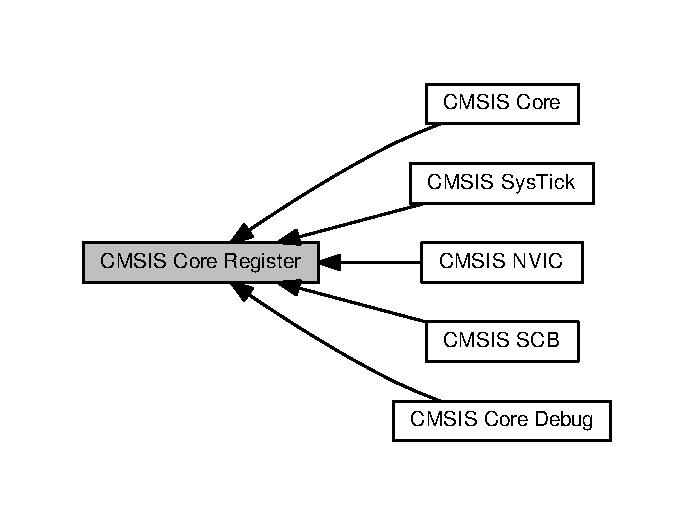
\includegraphics[width=333pt]{group___c_m_s_i_s__core__register}
\end{center}
\end{figure}
\subsection*{Modules}
\begin{DoxyCompactItemize}
\item 
\hyperlink{group___c_m_s_i_s___c_o_r_e}{C\+M\+S\+I\+S Core}
\item 
\hyperlink{group___c_m_s_i_s___n_v_i_c}{C\+M\+S\+I\+S N\+V\+IC}
\item 
\hyperlink{group___c_m_s_i_s___s_c_b}{C\+M\+S\+I\+S S\+CB}
\item 
\hyperlink{group___c_m_s_i_s___sys_tick}{C\+M\+S\+I\+S Sys\+Tick}
\item 
\hyperlink{group___c_m_s_i_s___core_debug}{C\+M\+S\+I\+S Core Debug}
\end{DoxyCompactItemize}
\begin{DoxyCompactItemize}
\item 
\#define \hyperlink{group___c_m_s_i_s__core__register_ga3c14ed93192c8d9143322bbf77ebf770}{S\+C\+S\+\_\+\+B\+A\+SE}~(0x\+E000\+E000\+U\+L)
\item 
\#define \hyperlink{group___c_m_s_i_s__core__register_ga680604dbcda9e9b31a1639fcffe5230b}{Core\+Debug\+\_\+\+B\+A\+SE}~(0x\+E000\+E\+D\+F0\+U\+L)
\item 
\#define \hyperlink{group___c_m_s_i_s__core__register_ga58effaac0b93006b756d33209e814646}{Sys\+Tick\+\_\+\+B\+A\+SE}~(\hyperlink{group___c_m_s_i_s__core__register_ga3c14ed93192c8d9143322bbf77ebf770}{S\+C\+S\+\_\+\+B\+A\+SE} +  0x0010\+U\+L)
\item 
\#define \hyperlink{group___c_m_s_i_s__core__register_gaa0288691785a5f868238e0468b39523d}{N\+V\+I\+C\+\_\+\+B\+A\+SE}~(\hyperlink{group___c_m_s_i_s__core__register_ga3c14ed93192c8d9143322bbf77ebf770}{S\+C\+S\+\_\+\+B\+A\+SE} +  0x0100\+U\+L)
\item 
\#define \hyperlink{group___c_m_s_i_s__core__register_gad55a7ddb8d4b2398b0c1cfec76c0d9fd}{S\+C\+B\+\_\+\+B\+A\+SE}~(\hyperlink{group___c_m_s_i_s__core__register_ga3c14ed93192c8d9143322bbf77ebf770}{S\+C\+S\+\_\+\+B\+A\+SE} +  0x0\+D00\+U\+L)
\item 
\#define \hyperlink{group___c_m_s_i_s__core__register_gaaaf6477c2bde2f00f99e3c2fd1060b01}{S\+CB}~((\hyperlink{struct_s_c_b___type}{S\+C\+B\+\_\+\+Type} $\ast$)           \hyperlink{group___c_m_s_i_s__core__register_gad55a7ddb8d4b2398b0c1cfec76c0d9fd}{S\+C\+B\+\_\+\+B\+A\+SE})
\item 
\#define \hyperlink{group___c_m_s_i_s__core__register_gacd96c53beeaff8f603fcda425eb295de}{Sys\+Tick}~((\hyperlink{struct_sys_tick___type}{Sys\+Tick\+\_\+\+Type} $\ast$)       \hyperlink{group___c_m_s_i_s__core__register_ga58effaac0b93006b756d33209e814646}{Sys\+Tick\+\_\+\+B\+A\+SE})
\item 
\#define \hyperlink{group___c_m_s_i_s__core__register_gac8e97e8ce56ae9f57da1363a937f8a17}{N\+V\+IC}~((\hyperlink{struct_n_v_i_c___type}{N\+V\+I\+C\+\_\+\+Type} $\ast$)          \hyperlink{group___c_m_s_i_s__core__register_gaa0288691785a5f868238e0468b39523d}{N\+V\+I\+C\+\_\+\+B\+A\+SE})
\end{DoxyCompactItemize}


\subsection{Detailed Description}
Core Register contain\+:
\begin{DoxyItemize}
\item Core Register
\item Core N\+V\+IC Register
\item Core S\+CB Register
\item Core Sys\+Tick Register 
\end{DoxyItemize}

\subsection{Macro Definition Documentation}
\index{C\+M\+S\+I\+S Core Register@{C\+M\+S\+I\+S Core Register}!Core\+Debug\+\_\+\+B\+A\+SE@{Core\+Debug\+\_\+\+B\+A\+SE}}
\index{Core\+Debug\+\_\+\+B\+A\+SE@{Core\+Debug\+\_\+\+B\+A\+SE}!C\+M\+S\+I\+S Core Register@{C\+M\+S\+I\+S Core Register}}
\subsubsection[{\texorpdfstring{Core\+Debug\+\_\+\+B\+A\+SE}{CoreDebug_BASE}}]{\setlength{\rightskip}{0pt plus 5cm}\#define Core\+Debug\+\_\+\+B\+A\+SE~(0x\+E000\+E\+D\+F0\+U\+L)}\hypertarget{group___c_m_s_i_s__core__register_ga680604dbcda9e9b31a1639fcffe5230b}{}\label{group___c_m_s_i_s__core__register_ga680604dbcda9e9b31a1639fcffe5230b}
Core Debug Base Address 

Definition at line 417 of file core\+\_\+cm0.\+h.

\index{C\+M\+S\+I\+S Core Register@{C\+M\+S\+I\+S Core Register}!N\+V\+IC@{N\+V\+IC}}
\index{N\+V\+IC@{N\+V\+IC}!C\+M\+S\+I\+S Core Register@{C\+M\+S\+I\+S Core Register}}
\subsubsection[{\texorpdfstring{N\+V\+IC}{NVIC}}]{\setlength{\rightskip}{0pt plus 5cm}\#define N\+V\+IC~(({\bf N\+V\+I\+C\+\_\+\+Type} $\ast$)          {\bf N\+V\+I\+C\+\_\+\+B\+A\+SE})}\hypertarget{group___c_m_s_i_s__core__register_gac8e97e8ce56ae9f57da1363a937f8a17}{}\label{group___c_m_s_i_s__core__register_gac8e97e8ce56ae9f57da1363a937f8a17}
N\+V\+IC configuration struct 

Definition at line 424 of file core\+\_\+cm0.\+h.

\index{C\+M\+S\+I\+S Core Register@{C\+M\+S\+I\+S Core Register}!N\+V\+I\+C\+\_\+\+B\+A\+SE@{N\+V\+I\+C\+\_\+\+B\+A\+SE}}
\index{N\+V\+I\+C\+\_\+\+B\+A\+SE@{N\+V\+I\+C\+\_\+\+B\+A\+SE}!C\+M\+S\+I\+S Core Register@{C\+M\+S\+I\+S Core Register}}
\subsubsection[{\texorpdfstring{N\+V\+I\+C\+\_\+\+B\+A\+SE}{NVIC_BASE}}]{\setlength{\rightskip}{0pt plus 5cm}\#define N\+V\+I\+C\+\_\+\+B\+A\+SE~({\bf S\+C\+S\+\_\+\+B\+A\+SE} +  0x0100\+U\+L)}\hypertarget{group___c_m_s_i_s__core__register_gaa0288691785a5f868238e0468b39523d}{}\label{group___c_m_s_i_s__core__register_gaa0288691785a5f868238e0468b39523d}
N\+V\+IC Base Address 

Definition at line 419 of file core\+\_\+cm0.\+h.

\index{C\+M\+S\+I\+S Core Register@{C\+M\+S\+I\+S Core Register}!S\+CB@{S\+CB}}
\index{S\+CB@{S\+CB}!C\+M\+S\+I\+S Core Register@{C\+M\+S\+I\+S Core Register}}
\subsubsection[{\texorpdfstring{S\+CB}{SCB}}]{\setlength{\rightskip}{0pt plus 5cm}\#define S\+CB~(({\bf S\+C\+B\+\_\+\+Type} $\ast$)           {\bf S\+C\+B\+\_\+\+B\+A\+SE})}\hypertarget{group___c_m_s_i_s__core__register_gaaaf6477c2bde2f00f99e3c2fd1060b01}{}\label{group___c_m_s_i_s__core__register_gaaaf6477c2bde2f00f99e3c2fd1060b01}
S\+CB configuration struct 

Definition at line 422 of file core\+\_\+cm0.\+h.

\index{C\+M\+S\+I\+S Core Register@{C\+M\+S\+I\+S Core Register}!S\+C\+B\+\_\+\+B\+A\+SE@{S\+C\+B\+\_\+\+B\+A\+SE}}
\index{S\+C\+B\+\_\+\+B\+A\+SE@{S\+C\+B\+\_\+\+B\+A\+SE}!C\+M\+S\+I\+S Core Register@{C\+M\+S\+I\+S Core Register}}
\subsubsection[{\texorpdfstring{S\+C\+B\+\_\+\+B\+A\+SE}{SCB_BASE}}]{\setlength{\rightskip}{0pt plus 5cm}\#define S\+C\+B\+\_\+\+B\+A\+SE~({\bf S\+C\+S\+\_\+\+B\+A\+SE} +  0x0\+D00\+U\+L)}\hypertarget{group___c_m_s_i_s__core__register_gad55a7ddb8d4b2398b0c1cfec76c0d9fd}{}\label{group___c_m_s_i_s__core__register_gad55a7ddb8d4b2398b0c1cfec76c0d9fd}
System Control Block Base Address 

Definition at line 420 of file core\+\_\+cm0.\+h.

\index{C\+M\+S\+I\+S Core Register@{C\+M\+S\+I\+S Core Register}!S\+C\+S\+\_\+\+B\+A\+SE@{S\+C\+S\+\_\+\+B\+A\+SE}}
\index{S\+C\+S\+\_\+\+B\+A\+SE@{S\+C\+S\+\_\+\+B\+A\+SE}!C\+M\+S\+I\+S Core Register@{C\+M\+S\+I\+S Core Register}}
\subsubsection[{\texorpdfstring{S\+C\+S\+\_\+\+B\+A\+SE}{SCS_BASE}}]{\setlength{\rightskip}{0pt plus 5cm}\#define S\+C\+S\+\_\+\+B\+A\+SE~(0x\+E000\+E000\+U\+L)}\hypertarget{group___c_m_s_i_s__core__register_ga3c14ed93192c8d9143322bbf77ebf770}{}\label{group___c_m_s_i_s__core__register_ga3c14ed93192c8d9143322bbf77ebf770}
System Control Space Base Address 

Definition at line 416 of file core\+\_\+cm0.\+h.

\index{C\+M\+S\+I\+S Core Register@{C\+M\+S\+I\+S Core Register}!Sys\+Tick@{Sys\+Tick}}
\index{Sys\+Tick@{Sys\+Tick}!C\+M\+S\+I\+S Core Register@{C\+M\+S\+I\+S Core Register}}
\subsubsection[{\texorpdfstring{Sys\+Tick}{SysTick}}]{\setlength{\rightskip}{0pt plus 5cm}\#define Sys\+Tick~(({\bf Sys\+Tick\+\_\+\+Type} $\ast$)       {\bf Sys\+Tick\+\_\+\+B\+A\+SE})}\hypertarget{group___c_m_s_i_s__core__register_gacd96c53beeaff8f603fcda425eb295de}{}\label{group___c_m_s_i_s__core__register_gacd96c53beeaff8f603fcda425eb295de}
Sys\+Tick configuration struct 

Definition at line 423 of file core\+\_\+cm0.\+h.

\index{C\+M\+S\+I\+S Core Register@{C\+M\+S\+I\+S Core Register}!Sys\+Tick\+\_\+\+B\+A\+SE@{Sys\+Tick\+\_\+\+B\+A\+SE}}
\index{Sys\+Tick\+\_\+\+B\+A\+SE@{Sys\+Tick\+\_\+\+B\+A\+SE}!C\+M\+S\+I\+S Core Register@{C\+M\+S\+I\+S Core Register}}
\subsubsection[{\texorpdfstring{Sys\+Tick\+\_\+\+B\+A\+SE}{SysTick_BASE}}]{\setlength{\rightskip}{0pt plus 5cm}\#define Sys\+Tick\+\_\+\+B\+A\+SE~({\bf S\+C\+S\+\_\+\+B\+A\+SE} +  0x0010\+U\+L)}\hypertarget{group___c_m_s_i_s__core__register_ga58effaac0b93006b756d33209e814646}{}\label{group___c_m_s_i_s__core__register_ga58effaac0b93006b756d33209e814646}
Sys\+Tick Base Address 

Definition at line 418 of file core\+\_\+cm0.\+h.


\hypertarget{group___c_m_s_i_s___c_o_r_e}{}\section{C\+M\+S\+IS Core}
\label{group___c_m_s_i_s___c_o_r_e}\index{C\+M\+S\+I\+S Core@{C\+M\+S\+I\+S Core}}
Collaboration diagram for C\+M\+S\+IS Core\+:\nopagebreak
\begin{figure}[H]
\begin{center}
\leavevmode
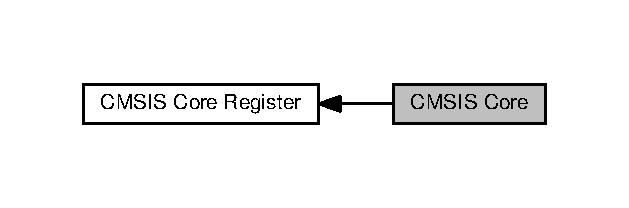
\includegraphics[width=302pt]{group___c_m_s_i_s___c_o_r_e}
\end{center}
\end{figure}
\subsection*{Classes}
\begin{DoxyCompactItemize}
\item 
union \hyperlink{union_a_p_s_r___type}{A\+P\+S\+R\+\_\+\+Type}
\begin{DoxyCompactList}\small\item\em Union type to access the Application Program Status Register (A\+P\+SR). \end{DoxyCompactList}\item 
union \hyperlink{union_i_p_s_r___type}{I\+P\+S\+R\+\_\+\+Type}
\begin{DoxyCompactList}\small\item\em Union type to access the Interrupt Program Status Register (I\+P\+SR). \end{DoxyCompactList}\item 
union \hyperlink{unionx_p_s_r___type}{x\+P\+S\+R\+\_\+\+Type}
\begin{DoxyCompactList}\small\item\em Union type to access the Special-\/\+Purpose Program Status Registers (x\+P\+SR). \end{DoxyCompactList}\item 
union \hyperlink{union_c_o_n_t_r_o_l___type}{C\+O\+N\+T\+R\+O\+L\+\_\+\+Type}
\begin{DoxyCompactList}\small\item\em Union type to access the Control Registers (C\+O\+N\+T\+R\+OL). \end{DoxyCompactList}\end{DoxyCompactItemize}


\subsection{Detailed Description}
Type definitions for the Cortex-\/M Core Registers 
\hypertarget{group___c_m_s_i_s___n_v_i_c}{}\section{C\+M\+S\+IS N\+V\+IC}
\label{group___c_m_s_i_s___n_v_i_c}\index{C\+M\+S\+I\+S N\+V\+IC@{C\+M\+S\+I\+S N\+V\+IC}}
Collaboration diagram for C\+M\+S\+IS N\+V\+IC\+:\nopagebreak
\begin{figure}[H]
\begin{center}
\leavevmode
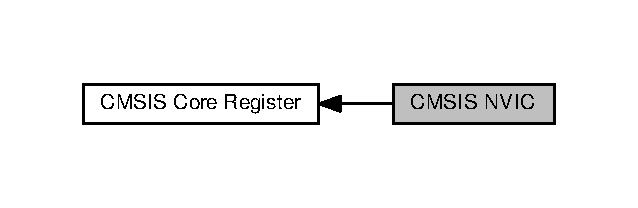
\includegraphics[width=306pt]{group___c_m_s_i_s___n_v_i_c}
\end{center}
\end{figure}
\subsection*{Classes}
\begin{DoxyCompactItemize}
\item 
struct \hyperlink{struct_n_v_i_c___type}{N\+V\+I\+C\+\_\+\+Type}
\begin{DoxyCompactList}\small\item\em Structure type to access the Nested Vectored Interrupt Controller (N\+V\+IC). \end{DoxyCompactList}\end{DoxyCompactItemize}


\subsection{Detailed Description}
Type definitions for the Cortex-\/M N\+V\+IC Registers 
\hypertarget{group___c_m_s_i_s___s_c_b}{}\section{C\+M\+S\+IS S\+CB}
\label{group___c_m_s_i_s___s_c_b}\index{C\+M\+S\+I\+S S\+CB@{C\+M\+S\+I\+S S\+CB}}
Collaboration diagram for C\+M\+S\+IS S\+CB\+:\nopagebreak
\begin{figure}[H]
\begin{center}
\leavevmode
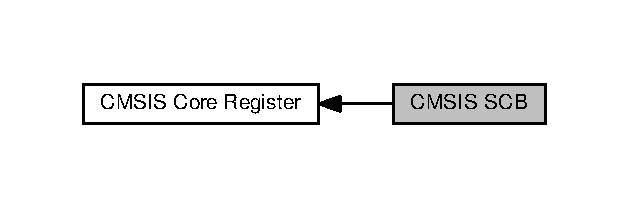
\includegraphics[width=302pt]{group___c_m_s_i_s___s_c_b}
\end{center}
\end{figure}
\subsection*{Classes}
\begin{DoxyCompactItemize}
\item 
struct \hyperlink{struct_s_c_b___type}{S\+C\+B\+\_\+\+Type}
\begin{DoxyCompactList}\small\item\em Structure type to access the System Control Block (S\+CB). \end{DoxyCompactList}\end{DoxyCompactItemize}
\subsection*{Macros}
\begin{DoxyCompactItemize}
\item 
\#define \hyperlink{group___c_m_s_i_s___s_c_b_ga58686b88f94f789d4e6f429fe1ff58cf}{S\+C\+B\+\_\+\+C\+P\+U\+I\+D\+\_\+\+I\+M\+P\+L\+E\+M\+E\+N\+T\+E\+R\+\_\+\+Pos}~24
\item 
\#define \hyperlink{group___c_m_s_i_s___s_c_b_ga0932b31faafd47656a03ced75a31d99b}{S\+C\+B\+\_\+\+C\+P\+U\+I\+D\+\_\+\+I\+M\+P\+L\+E\+M\+E\+N\+T\+E\+R\+\_\+\+Msk}~(0x\+F\+F\+U\+L $<$$<$ S\+C\+B\+\_\+\+C\+P\+U\+I\+D\+\_\+\+I\+M\+P\+L\+E\+M\+E\+N\+T\+E\+R\+\_\+\+Pos)
\item 
\#define \hyperlink{group___c_m_s_i_s___s_c_b_ga104462bd0815391b4044a70bd15d3a71}{S\+C\+B\+\_\+\+C\+P\+U\+I\+D\+\_\+\+V\+A\+R\+I\+A\+N\+T\+\_\+\+Pos}~20
\item 
\#define \hyperlink{group___c_m_s_i_s___s_c_b_gad358dfbd04300afc1824329d128b99e8}{S\+C\+B\+\_\+\+C\+P\+U\+I\+D\+\_\+\+V\+A\+R\+I\+A\+N\+T\+\_\+\+Msk}~(0x\+F\+U\+L $<$$<$ S\+C\+B\+\_\+\+C\+P\+U\+I\+D\+\_\+\+V\+A\+R\+I\+A\+N\+T\+\_\+\+Pos)
\item 
\#define \hyperlink{group___c_m_s_i_s___s_c_b_gaf8b3236b08fb8e840efb682645fb0e98}{S\+C\+B\+\_\+\+C\+P\+U\+I\+D\+\_\+\+A\+R\+C\+H\+I\+T\+E\+C\+T\+U\+R\+E\+\_\+\+Pos}~16
\item 
\#define \hyperlink{group___c_m_s_i_s___s_c_b_gafae4a1f27a927338ae9dc51a0e146213}{S\+C\+B\+\_\+\+C\+P\+U\+I\+D\+\_\+\+A\+R\+C\+H\+I\+T\+E\+C\+T\+U\+R\+E\+\_\+\+Msk}~(0x\+F\+U\+L $<$$<$ S\+C\+B\+\_\+\+C\+P\+U\+I\+D\+\_\+\+A\+R\+C\+H\+I\+T\+E\+C\+T\+U\+R\+E\+\_\+\+Pos)
\item 
\#define \hyperlink{group___c_m_s_i_s___s_c_b_ga705f68eaa9afb042ca2407dc4e4629ac}{S\+C\+B\+\_\+\+C\+P\+U\+I\+D\+\_\+\+P\+A\+R\+T\+N\+O\+\_\+\+Pos}~4
\item 
\#define \hyperlink{group___c_m_s_i_s___s_c_b_ga98e581423ca016680c238c469aba546d}{S\+C\+B\+\_\+\+C\+P\+U\+I\+D\+\_\+\+P\+A\+R\+T\+N\+O\+\_\+\+Msk}~(0x\+F\+F\+F\+U\+L $<$$<$ S\+C\+B\+\_\+\+C\+P\+U\+I\+D\+\_\+\+P\+A\+R\+T\+N\+O\+\_\+\+Pos)
\item 
\#define \hyperlink{group___c_m_s_i_s___s_c_b_ga3c3d9071e574de11fb27ba57034838b1}{S\+C\+B\+\_\+\+C\+P\+U\+I\+D\+\_\+\+R\+E\+V\+I\+S\+I\+O\+N\+\_\+\+Pos}~0
\item 
\#define \hyperlink{group___c_m_s_i_s___s_c_b_ga2ec0448b6483f77e7f5d08b4b81d85df}{S\+C\+B\+\_\+\+C\+P\+U\+I\+D\+\_\+\+R\+E\+V\+I\+S\+I\+O\+N\+\_\+\+Msk}~(0x\+F\+U\+L $<$$<$ S\+C\+B\+\_\+\+C\+P\+U\+I\+D\+\_\+\+R\+E\+V\+I\+S\+I\+O\+N\+\_\+\+Pos)
\item 
\#define \hyperlink{group___c_m_s_i_s___s_c_b_ga750d4b52624a46d71356db4ea769573b}{S\+C\+B\+\_\+\+I\+C\+S\+R\+\_\+\+N\+M\+I\+P\+E\+N\+D\+S\+E\+T\+\_\+\+Pos}~31
\item 
\#define \hyperlink{group___c_m_s_i_s___s_c_b_ga340e3f79e9c3607dee9f2c048b6b22e8}{S\+C\+B\+\_\+\+I\+C\+S\+R\+\_\+\+N\+M\+I\+P\+E\+N\+D\+S\+E\+T\+\_\+\+Msk}~(1\+U\+L $<$$<$ S\+C\+B\+\_\+\+I\+C\+S\+R\+\_\+\+N\+M\+I\+P\+E\+N\+D\+S\+E\+T\+\_\+\+Pos)
\item 
\#define \hyperlink{group___c_m_s_i_s___s_c_b_gab5ded23d2ab1d5ff7cc7ce746205e9fe}{S\+C\+B\+\_\+\+I\+C\+S\+R\+\_\+\+P\+E\+N\+D\+S\+V\+S\+E\+T\+\_\+\+Pos}~28
\item 
\#define \hyperlink{group___c_m_s_i_s___s_c_b_ga1e40d93efb402763c8c00ddcc56724ff}{S\+C\+B\+\_\+\+I\+C\+S\+R\+\_\+\+P\+E\+N\+D\+S\+V\+S\+E\+T\+\_\+\+Msk}~(1\+U\+L $<$$<$ S\+C\+B\+\_\+\+I\+C\+S\+R\+\_\+\+P\+E\+N\+D\+S\+V\+S\+E\+T\+\_\+\+Pos)
\item 
\#define \hyperlink{group___c_m_s_i_s___s_c_b_gae218d9022288f89faf57187c4d542ecd}{S\+C\+B\+\_\+\+I\+C\+S\+R\+\_\+\+P\+E\+N\+D\+S\+V\+C\+L\+R\+\_\+\+Pos}~27
\item 
\#define \hyperlink{group___c_m_s_i_s___s_c_b_ga4a901ace381d3c1c74ac82b22fae2e1e}{S\+C\+B\+\_\+\+I\+C\+S\+R\+\_\+\+P\+E\+N\+D\+S\+V\+C\+L\+R\+\_\+\+Msk}~(1\+U\+L $<$$<$ S\+C\+B\+\_\+\+I\+C\+S\+R\+\_\+\+P\+E\+N\+D\+S\+V\+C\+L\+R\+\_\+\+Pos)
\item 
\#define \hyperlink{group___c_m_s_i_s___s_c_b_ga9dbb3358c6167c9c3f85661b90fb2794}{S\+C\+B\+\_\+\+I\+C\+S\+R\+\_\+\+P\+E\+N\+D\+S\+T\+S\+E\+T\+\_\+\+Pos}~26
\item 
\#define \hyperlink{group___c_m_s_i_s___s_c_b_ga7325b61ea0ec323ef2d5c893b112e546}{S\+C\+B\+\_\+\+I\+C\+S\+R\+\_\+\+P\+E\+N\+D\+S\+T\+S\+E\+T\+\_\+\+Msk}~(1\+U\+L $<$$<$ S\+C\+B\+\_\+\+I\+C\+S\+R\+\_\+\+P\+E\+N\+D\+S\+T\+S\+E\+T\+\_\+\+Pos)
\item 
\#define \hyperlink{group___c_m_s_i_s___s_c_b_gadbe25e4b333ece1341beb1a740168fdc}{S\+C\+B\+\_\+\+I\+C\+S\+R\+\_\+\+P\+E\+N\+D\+S\+T\+C\+L\+R\+\_\+\+Pos}~25
\item 
\#define \hyperlink{group___c_m_s_i_s___s_c_b_gab241827d2a793269d8cd99b9b28c2157}{S\+C\+B\+\_\+\+I\+C\+S\+R\+\_\+\+P\+E\+N\+D\+S\+T\+C\+L\+R\+\_\+\+Msk}~(1\+U\+L $<$$<$ S\+C\+B\+\_\+\+I\+C\+S\+R\+\_\+\+P\+E\+N\+D\+S\+T\+C\+L\+R\+\_\+\+Pos)
\item 
\#define \hyperlink{group___c_m_s_i_s___s_c_b_ga11cb5b1f9ce167b81f31787a77e575df}{S\+C\+B\+\_\+\+I\+C\+S\+R\+\_\+\+I\+S\+R\+P\+R\+E\+E\+M\+P\+T\+\_\+\+Pos}~23
\item 
\#define \hyperlink{group___c_m_s_i_s___s_c_b_gaa966600396290808d596fe96e92ca2b5}{S\+C\+B\+\_\+\+I\+C\+S\+R\+\_\+\+I\+S\+R\+P\+R\+E\+E\+M\+P\+T\+\_\+\+Msk}~(1\+U\+L $<$$<$ S\+C\+B\+\_\+\+I\+C\+S\+R\+\_\+\+I\+S\+R\+P\+R\+E\+E\+M\+P\+T\+\_\+\+Pos)
\item 
\#define \hyperlink{group___c_m_s_i_s___s_c_b_ga10749d92b9b744094b845c2eb46d4319}{S\+C\+B\+\_\+\+I\+C\+S\+R\+\_\+\+I\+S\+R\+P\+E\+N\+D\+I\+N\+G\+\_\+\+Pos}~22
\item 
\#define \hyperlink{group___c_m_s_i_s___s_c_b_ga056d74fd538e5d36d3be1f28d399c877}{S\+C\+B\+\_\+\+I\+C\+S\+R\+\_\+\+I\+S\+R\+P\+E\+N\+D\+I\+N\+G\+\_\+\+Msk}~(1\+U\+L $<$$<$ S\+C\+B\+\_\+\+I\+C\+S\+R\+\_\+\+I\+S\+R\+P\+E\+N\+D\+I\+N\+G\+\_\+\+Pos)
\item 
\#define \hyperlink{group___c_m_s_i_s___s_c_b_gada60c92bf88d6fd21a8f49efa4a127b8}{S\+C\+B\+\_\+\+I\+C\+S\+R\+\_\+\+V\+E\+C\+T\+P\+E\+N\+D\+I\+N\+G\+\_\+\+Pos}~12
\item 
\#define \hyperlink{group___c_m_s_i_s___s_c_b_gacb6992e7c7ddc27a370f62878a21ef72}{S\+C\+B\+\_\+\+I\+C\+S\+R\+\_\+\+V\+E\+C\+T\+P\+E\+N\+D\+I\+N\+G\+\_\+\+Msk}~(0x1\+F\+F\+U\+L $<$$<$ S\+C\+B\+\_\+\+I\+C\+S\+R\+\_\+\+V\+E\+C\+T\+P\+E\+N\+D\+I\+N\+G\+\_\+\+Pos)
\item 
\#define \hyperlink{group___c_m_s_i_s___s_c_b_gae4f602c7c5c895d5fb687b71b0979fc3}{S\+C\+B\+\_\+\+I\+C\+S\+R\+\_\+\+V\+E\+C\+T\+A\+C\+T\+I\+V\+E\+\_\+\+Pos}~0
\item 
\#define \hyperlink{group___c_m_s_i_s___s_c_b_ga5533791a4ecf1b9301c883047b3e8396}{S\+C\+B\+\_\+\+I\+C\+S\+R\+\_\+\+V\+E\+C\+T\+A\+C\+T\+I\+V\+E\+\_\+\+Msk}~(0x1\+F\+F\+U\+L $<$$<$ S\+C\+B\+\_\+\+I\+C\+S\+R\+\_\+\+V\+E\+C\+T\+A\+C\+T\+I\+V\+E\+\_\+\+Pos)
\item 
\#define \hyperlink{group___c_m_s_i_s___s_c_b_gaaa27c0ba600bf82c3da08c748845b640}{S\+C\+B\+\_\+\+A\+I\+R\+C\+R\+\_\+\+V\+E\+C\+T\+K\+E\+Y\+\_\+\+Pos}~16
\item 
\#define \hyperlink{group___c_m_s_i_s___s_c_b_ga90c7cf0c490e7ae55f9503a7fda1dd22}{S\+C\+B\+\_\+\+A\+I\+R\+C\+R\+\_\+\+V\+E\+C\+T\+K\+E\+Y\+\_\+\+Msk}~(0x\+F\+F\+F\+F\+U\+L $<$$<$ S\+C\+B\+\_\+\+A\+I\+R\+C\+R\+\_\+\+V\+E\+C\+T\+K\+E\+Y\+\_\+\+Pos)
\item 
\#define \hyperlink{group___c_m_s_i_s___s_c_b_gaec404750ff5ca07f499a3c06b62051ef}{S\+C\+B\+\_\+\+A\+I\+R\+C\+R\+\_\+\+V\+E\+C\+T\+K\+E\+Y\+S\+T\+A\+T\+\_\+\+Pos}~16
\item 
\#define \hyperlink{group___c_m_s_i_s___s_c_b_gabacedaefeefc73d666bbe59ece904493}{S\+C\+B\+\_\+\+A\+I\+R\+C\+R\+\_\+\+V\+E\+C\+T\+K\+E\+Y\+S\+T\+A\+T\+\_\+\+Msk}~(0x\+F\+F\+F\+F\+U\+L $<$$<$ S\+C\+B\+\_\+\+A\+I\+R\+C\+R\+\_\+\+V\+E\+C\+T\+K\+E\+Y\+S\+T\+A\+T\+\_\+\+Pos)
\item 
\#define \hyperlink{group___c_m_s_i_s___s_c_b_gad31dec98fbc0d33ace63cb1f1a927923}{S\+C\+B\+\_\+\+A\+I\+R\+C\+R\+\_\+\+E\+N\+D\+I\+A\+N\+E\+S\+S\+\_\+\+Pos}~15
\item 
\#define \hyperlink{group___c_m_s_i_s___s_c_b_ga2f571f93d3d4a6eac9a3040756d3d951}{S\+C\+B\+\_\+\+A\+I\+R\+C\+R\+\_\+\+E\+N\+D\+I\+A\+N\+E\+S\+S\+\_\+\+Msk}~(1\+U\+L $<$$<$ S\+C\+B\+\_\+\+A\+I\+R\+C\+R\+\_\+\+E\+N\+D\+I\+A\+N\+E\+S\+S\+\_\+\+Pos)
\item 
\#define \hyperlink{group___c_m_s_i_s___s_c_b_gaffb2737eca1eac0fc1c282a76a40953c}{S\+C\+B\+\_\+\+A\+I\+R\+C\+R\+\_\+\+S\+Y\+S\+R\+E\+S\+E\+T\+R\+E\+Q\+\_\+\+Pos}~2
\item 
\#define \hyperlink{group___c_m_s_i_s___s_c_b_gaae1181119559a5bd36e62afa373fa720}{S\+C\+B\+\_\+\+A\+I\+R\+C\+R\+\_\+\+S\+Y\+S\+R\+E\+S\+E\+T\+R\+E\+Q\+\_\+\+Msk}~(1\+U\+L $<$$<$ S\+C\+B\+\_\+\+A\+I\+R\+C\+R\+\_\+\+S\+Y\+S\+R\+E\+S\+E\+T\+R\+E\+Q\+\_\+\+Pos)
\item 
\#define \hyperlink{group___c_m_s_i_s___s_c_b_gaa30a12e892bb696e61626d71359a9029}{S\+C\+B\+\_\+\+A\+I\+R\+C\+R\+\_\+\+V\+E\+C\+T\+C\+L\+R\+A\+C\+T\+I\+V\+E\+\_\+\+Pos}~1
\item 
\#define \hyperlink{group___c_m_s_i_s___s_c_b_ga212c5ab1c1c82c807d30d2307aa8d218}{S\+C\+B\+\_\+\+A\+I\+R\+C\+R\+\_\+\+V\+E\+C\+T\+C\+L\+R\+A\+C\+T\+I\+V\+E\+\_\+\+Msk}~(1\+U\+L $<$$<$ S\+C\+B\+\_\+\+A\+I\+R\+C\+R\+\_\+\+V\+E\+C\+T\+C\+L\+R\+A\+C\+T\+I\+V\+E\+\_\+\+Pos)
\item 
\#define \hyperlink{group___c_m_s_i_s___s_c_b_ga3bddcec40aeaf3d3a998446100fa0e44}{S\+C\+B\+\_\+\+S\+C\+R\+\_\+\+S\+E\+V\+O\+N\+P\+E\+N\+D\+\_\+\+Pos}~4
\item 
\#define \hyperlink{group___c_m_s_i_s___s_c_b_gafb98656644a14342e467505f69a997c9}{S\+C\+B\+\_\+\+S\+C\+R\+\_\+\+S\+E\+V\+O\+N\+P\+E\+N\+D\+\_\+\+Msk}~(1\+U\+L $<$$<$ S\+C\+B\+\_\+\+S\+C\+R\+\_\+\+S\+E\+V\+O\+N\+P\+E\+N\+D\+\_\+\+Pos)
\item 
\#define \hyperlink{group___c_m_s_i_s___s_c_b_gab304f6258ec03bd9a6e7a360515c3cfe}{S\+C\+B\+\_\+\+S\+C\+R\+\_\+\+S\+L\+E\+E\+P\+D\+E\+E\+P\+\_\+\+Pos}~2
\item 
\#define \hyperlink{group___c_m_s_i_s___s_c_b_ga77c06a69c63f4b3f6ec1032e911e18e7}{S\+C\+B\+\_\+\+S\+C\+R\+\_\+\+S\+L\+E\+E\+P\+D\+E\+E\+P\+\_\+\+Msk}~(1\+U\+L $<$$<$ S\+C\+B\+\_\+\+S\+C\+R\+\_\+\+S\+L\+E\+E\+P\+D\+E\+E\+P\+\_\+\+Pos)
\item 
\#define \hyperlink{group___c_m_s_i_s___s_c_b_ga3680a15114d7fdc1e25043b881308fe9}{S\+C\+B\+\_\+\+S\+C\+R\+\_\+\+S\+L\+E\+E\+P\+O\+N\+E\+X\+I\+T\+\_\+\+Pos}~1
\item 
\#define \hyperlink{group___c_m_s_i_s___s_c_b_ga50a243e317b9a70781b02758d45b05ee}{S\+C\+B\+\_\+\+S\+C\+R\+\_\+\+S\+L\+E\+E\+P\+O\+N\+E\+X\+I\+T\+\_\+\+Msk}~(1\+U\+L $<$$<$ S\+C\+B\+\_\+\+S\+C\+R\+\_\+\+S\+L\+E\+E\+P\+O\+N\+E\+X\+I\+T\+\_\+\+Pos)
\item 
\#define \hyperlink{group___c_m_s_i_s___s_c_b_gac2d20a250960a432cc74da59d20e2f86}{S\+C\+B\+\_\+\+C\+C\+R\+\_\+\+S\+T\+K\+A\+L\+I\+G\+N\+\_\+\+Pos}~9
\item 
\#define \hyperlink{group___c_m_s_i_s___s_c_b_ga33cf22d3d46af158a03aad25ddea1bcb}{S\+C\+B\+\_\+\+C\+C\+R\+\_\+\+S\+T\+K\+A\+L\+I\+G\+N\+\_\+\+Msk}~(1\+U\+L $<$$<$ S\+C\+B\+\_\+\+C\+C\+R\+\_\+\+S\+T\+K\+A\+L\+I\+G\+N\+\_\+\+Pos)
\item 
\#define \hyperlink{group___c_m_s_i_s___s_c_b_gac4e4928b864ea10fc24dbbc57d976229}{S\+C\+B\+\_\+\+C\+C\+R\+\_\+\+U\+N\+A\+L\+I\+G\+N\+\_\+\+T\+R\+P\+\_\+\+Pos}~3
\item 
\#define \hyperlink{group___c_m_s_i_s___s_c_b_ga68c96ad594af70c007923979085c99e0}{S\+C\+B\+\_\+\+C\+C\+R\+\_\+\+U\+N\+A\+L\+I\+G\+N\+\_\+\+T\+R\+P\+\_\+\+Msk}~(1\+U\+L $<$$<$ S\+C\+B\+\_\+\+C\+C\+R\+\_\+\+U\+N\+A\+L\+I\+G\+N\+\_\+\+T\+R\+P\+\_\+\+Pos)
\end{DoxyCompactItemize}


\subsection{Detailed Description}
Type definitions for the Cortex-\/M System Control Block Registers 

\subsection{Macro Definition Documentation}
\index{C\+M\+S\+I\+S S\+CB@{C\+M\+S\+I\+S S\+CB}!S\+C\+B\+\_\+\+A\+I\+R\+C\+R\+\_\+\+E\+N\+D\+I\+A\+N\+E\+S\+S\+\_\+\+Msk@{S\+C\+B\+\_\+\+A\+I\+R\+C\+R\+\_\+\+E\+N\+D\+I\+A\+N\+E\+S\+S\+\_\+\+Msk}}
\index{S\+C\+B\+\_\+\+A\+I\+R\+C\+R\+\_\+\+E\+N\+D\+I\+A\+N\+E\+S\+S\+\_\+\+Msk@{S\+C\+B\+\_\+\+A\+I\+R\+C\+R\+\_\+\+E\+N\+D\+I\+A\+N\+E\+S\+S\+\_\+\+Msk}!C\+M\+S\+I\+S S\+CB@{C\+M\+S\+I\+S S\+CB}}
\subsubsection[{\texorpdfstring{S\+C\+B\+\_\+\+A\+I\+R\+C\+R\+\_\+\+E\+N\+D\+I\+A\+N\+E\+S\+S\+\_\+\+Msk}{SCB_AIRCR_ENDIANESS_Msk}}]{\setlength{\rightskip}{0pt plus 5cm}\#define S\+C\+B\+\_\+\+A\+I\+R\+C\+R\+\_\+\+E\+N\+D\+I\+A\+N\+E\+S\+S\+\_\+\+Msk~(1\+U\+L $<$$<$ S\+C\+B\+\_\+\+A\+I\+R\+C\+R\+\_\+\+E\+N\+D\+I\+A\+N\+E\+S\+S\+\_\+\+Pos)}\hypertarget{group___c_m_s_i_s___s_c_b_ga2f571f93d3d4a6eac9a3040756d3d951}{}\label{group___c_m_s_i_s___s_c_b_ga2f571f93d3d4a6eac9a3040756d3d951}
S\+CB A\+I\+R\+CR\+: E\+N\+D\+I\+A\+N\+E\+SS Mask 

Definition at line 323 of file core\+\_\+cm0.\+h.

\index{C\+M\+S\+I\+S S\+CB@{C\+M\+S\+I\+S S\+CB}!S\+C\+B\+\_\+\+A\+I\+R\+C\+R\+\_\+\+E\+N\+D\+I\+A\+N\+E\+S\+S\+\_\+\+Pos@{S\+C\+B\+\_\+\+A\+I\+R\+C\+R\+\_\+\+E\+N\+D\+I\+A\+N\+E\+S\+S\+\_\+\+Pos}}
\index{S\+C\+B\+\_\+\+A\+I\+R\+C\+R\+\_\+\+E\+N\+D\+I\+A\+N\+E\+S\+S\+\_\+\+Pos@{S\+C\+B\+\_\+\+A\+I\+R\+C\+R\+\_\+\+E\+N\+D\+I\+A\+N\+E\+S\+S\+\_\+\+Pos}!C\+M\+S\+I\+S S\+CB@{C\+M\+S\+I\+S S\+CB}}
\subsubsection[{\texorpdfstring{S\+C\+B\+\_\+\+A\+I\+R\+C\+R\+\_\+\+E\+N\+D\+I\+A\+N\+E\+S\+S\+\_\+\+Pos}{SCB_AIRCR_ENDIANESS_Pos}}]{\setlength{\rightskip}{0pt plus 5cm}\#define S\+C\+B\+\_\+\+A\+I\+R\+C\+R\+\_\+\+E\+N\+D\+I\+A\+N\+E\+S\+S\+\_\+\+Pos~15}\hypertarget{group___c_m_s_i_s___s_c_b_gad31dec98fbc0d33ace63cb1f1a927923}{}\label{group___c_m_s_i_s___s_c_b_gad31dec98fbc0d33ace63cb1f1a927923}
S\+CB A\+I\+R\+CR\+: E\+N\+D\+I\+A\+N\+E\+SS Position 

Definition at line 322 of file core\+\_\+cm0.\+h.

\index{C\+M\+S\+I\+S S\+CB@{C\+M\+S\+I\+S S\+CB}!S\+C\+B\+\_\+\+A\+I\+R\+C\+R\+\_\+\+S\+Y\+S\+R\+E\+S\+E\+T\+R\+E\+Q\+\_\+\+Msk@{S\+C\+B\+\_\+\+A\+I\+R\+C\+R\+\_\+\+S\+Y\+S\+R\+E\+S\+E\+T\+R\+E\+Q\+\_\+\+Msk}}
\index{S\+C\+B\+\_\+\+A\+I\+R\+C\+R\+\_\+\+S\+Y\+S\+R\+E\+S\+E\+T\+R\+E\+Q\+\_\+\+Msk@{S\+C\+B\+\_\+\+A\+I\+R\+C\+R\+\_\+\+S\+Y\+S\+R\+E\+S\+E\+T\+R\+E\+Q\+\_\+\+Msk}!C\+M\+S\+I\+S S\+CB@{C\+M\+S\+I\+S S\+CB}}
\subsubsection[{\texorpdfstring{S\+C\+B\+\_\+\+A\+I\+R\+C\+R\+\_\+\+S\+Y\+S\+R\+E\+S\+E\+T\+R\+E\+Q\+\_\+\+Msk}{SCB_AIRCR_SYSRESETREQ_Msk}}]{\setlength{\rightskip}{0pt plus 5cm}\#define S\+C\+B\+\_\+\+A\+I\+R\+C\+R\+\_\+\+S\+Y\+S\+R\+E\+S\+E\+T\+R\+E\+Q\+\_\+\+Msk~(1\+U\+L $<$$<$ S\+C\+B\+\_\+\+A\+I\+R\+C\+R\+\_\+\+S\+Y\+S\+R\+E\+S\+E\+T\+R\+E\+Q\+\_\+\+Pos)}\hypertarget{group___c_m_s_i_s___s_c_b_gaae1181119559a5bd36e62afa373fa720}{}\label{group___c_m_s_i_s___s_c_b_gaae1181119559a5bd36e62afa373fa720}
S\+CB A\+I\+R\+CR\+: S\+Y\+S\+R\+E\+S\+E\+T\+R\+EQ Mask 

Definition at line 326 of file core\+\_\+cm0.\+h.

\index{C\+M\+S\+I\+S S\+CB@{C\+M\+S\+I\+S S\+CB}!S\+C\+B\+\_\+\+A\+I\+R\+C\+R\+\_\+\+S\+Y\+S\+R\+E\+S\+E\+T\+R\+E\+Q\+\_\+\+Pos@{S\+C\+B\+\_\+\+A\+I\+R\+C\+R\+\_\+\+S\+Y\+S\+R\+E\+S\+E\+T\+R\+E\+Q\+\_\+\+Pos}}
\index{S\+C\+B\+\_\+\+A\+I\+R\+C\+R\+\_\+\+S\+Y\+S\+R\+E\+S\+E\+T\+R\+E\+Q\+\_\+\+Pos@{S\+C\+B\+\_\+\+A\+I\+R\+C\+R\+\_\+\+S\+Y\+S\+R\+E\+S\+E\+T\+R\+E\+Q\+\_\+\+Pos}!C\+M\+S\+I\+S S\+CB@{C\+M\+S\+I\+S S\+CB}}
\subsubsection[{\texorpdfstring{S\+C\+B\+\_\+\+A\+I\+R\+C\+R\+\_\+\+S\+Y\+S\+R\+E\+S\+E\+T\+R\+E\+Q\+\_\+\+Pos}{SCB_AIRCR_SYSRESETREQ_Pos}}]{\setlength{\rightskip}{0pt plus 5cm}\#define S\+C\+B\+\_\+\+A\+I\+R\+C\+R\+\_\+\+S\+Y\+S\+R\+E\+S\+E\+T\+R\+E\+Q\+\_\+\+Pos~2}\hypertarget{group___c_m_s_i_s___s_c_b_gaffb2737eca1eac0fc1c282a76a40953c}{}\label{group___c_m_s_i_s___s_c_b_gaffb2737eca1eac0fc1c282a76a40953c}
S\+CB A\+I\+R\+CR\+: S\+Y\+S\+R\+E\+S\+E\+T\+R\+EQ Position 

Definition at line 325 of file core\+\_\+cm0.\+h.

\index{C\+M\+S\+I\+S S\+CB@{C\+M\+S\+I\+S S\+CB}!S\+C\+B\+\_\+\+A\+I\+R\+C\+R\+\_\+\+V\+E\+C\+T\+C\+L\+R\+A\+C\+T\+I\+V\+E\+\_\+\+Msk@{S\+C\+B\+\_\+\+A\+I\+R\+C\+R\+\_\+\+V\+E\+C\+T\+C\+L\+R\+A\+C\+T\+I\+V\+E\+\_\+\+Msk}}
\index{S\+C\+B\+\_\+\+A\+I\+R\+C\+R\+\_\+\+V\+E\+C\+T\+C\+L\+R\+A\+C\+T\+I\+V\+E\+\_\+\+Msk@{S\+C\+B\+\_\+\+A\+I\+R\+C\+R\+\_\+\+V\+E\+C\+T\+C\+L\+R\+A\+C\+T\+I\+V\+E\+\_\+\+Msk}!C\+M\+S\+I\+S S\+CB@{C\+M\+S\+I\+S S\+CB}}
\subsubsection[{\texorpdfstring{S\+C\+B\+\_\+\+A\+I\+R\+C\+R\+\_\+\+V\+E\+C\+T\+C\+L\+R\+A\+C\+T\+I\+V\+E\+\_\+\+Msk}{SCB_AIRCR_VECTCLRACTIVE_Msk}}]{\setlength{\rightskip}{0pt plus 5cm}\#define S\+C\+B\+\_\+\+A\+I\+R\+C\+R\+\_\+\+V\+E\+C\+T\+C\+L\+R\+A\+C\+T\+I\+V\+E\+\_\+\+Msk~(1\+U\+L $<$$<$ S\+C\+B\+\_\+\+A\+I\+R\+C\+R\+\_\+\+V\+E\+C\+T\+C\+L\+R\+A\+C\+T\+I\+V\+E\+\_\+\+Pos)}\hypertarget{group___c_m_s_i_s___s_c_b_ga212c5ab1c1c82c807d30d2307aa8d218}{}\label{group___c_m_s_i_s___s_c_b_ga212c5ab1c1c82c807d30d2307aa8d218}
S\+CB A\+I\+R\+CR\+: V\+E\+C\+T\+C\+L\+R\+A\+C\+T\+I\+VE Mask 

Definition at line 329 of file core\+\_\+cm0.\+h.

\index{C\+M\+S\+I\+S S\+CB@{C\+M\+S\+I\+S S\+CB}!S\+C\+B\+\_\+\+A\+I\+R\+C\+R\+\_\+\+V\+E\+C\+T\+C\+L\+R\+A\+C\+T\+I\+V\+E\+\_\+\+Pos@{S\+C\+B\+\_\+\+A\+I\+R\+C\+R\+\_\+\+V\+E\+C\+T\+C\+L\+R\+A\+C\+T\+I\+V\+E\+\_\+\+Pos}}
\index{S\+C\+B\+\_\+\+A\+I\+R\+C\+R\+\_\+\+V\+E\+C\+T\+C\+L\+R\+A\+C\+T\+I\+V\+E\+\_\+\+Pos@{S\+C\+B\+\_\+\+A\+I\+R\+C\+R\+\_\+\+V\+E\+C\+T\+C\+L\+R\+A\+C\+T\+I\+V\+E\+\_\+\+Pos}!C\+M\+S\+I\+S S\+CB@{C\+M\+S\+I\+S S\+CB}}
\subsubsection[{\texorpdfstring{S\+C\+B\+\_\+\+A\+I\+R\+C\+R\+\_\+\+V\+E\+C\+T\+C\+L\+R\+A\+C\+T\+I\+V\+E\+\_\+\+Pos}{SCB_AIRCR_VECTCLRACTIVE_Pos}}]{\setlength{\rightskip}{0pt plus 5cm}\#define S\+C\+B\+\_\+\+A\+I\+R\+C\+R\+\_\+\+V\+E\+C\+T\+C\+L\+R\+A\+C\+T\+I\+V\+E\+\_\+\+Pos~1}\hypertarget{group___c_m_s_i_s___s_c_b_gaa30a12e892bb696e61626d71359a9029}{}\label{group___c_m_s_i_s___s_c_b_gaa30a12e892bb696e61626d71359a9029}
S\+CB A\+I\+R\+CR\+: V\+E\+C\+T\+C\+L\+R\+A\+C\+T\+I\+VE Position 

Definition at line 328 of file core\+\_\+cm0.\+h.

\index{C\+M\+S\+I\+S S\+CB@{C\+M\+S\+I\+S S\+CB}!S\+C\+B\+\_\+\+A\+I\+R\+C\+R\+\_\+\+V\+E\+C\+T\+K\+E\+Y\+\_\+\+Msk@{S\+C\+B\+\_\+\+A\+I\+R\+C\+R\+\_\+\+V\+E\+C\+T\+K\+E\+Y\+\_\+\+Msk}}
\index{S\+C\+B\+\_\+\+A\+I\+R\+C\+R\+\_\+\+V\+E\+C\+T\+K\+E\+Y\+\_\+\+Msk@{S\+C\+B\+\_\+\+A\+I\+R\+C\+R\+\_\+\+V\+E\+C\+T\+K\+E\+Y\+\_\+\+Msk}!C\+M\+S\+I\+S S\+CB@{C\+M\+S\+I\+S S\+CB}}
\subsubsection[{\texorpdfstring{S\+C\+B\+\_\+\+A\+I\+R\+C\+R\+\_\+\+V\+E\+C\+T\+K\+E\+Y\+\_\+\+Msk}{SCB_AIRCR_VECTKEY_Msk}}]{\setlength{\rightskip}{0pt plus 5cm}\#define S\+C\+B\+\_\+\+A\+I\+R\+C\+R\+\_\+\+V\+E\+C\+T\+K\+E\+Y\+\_\+\+Msk~(0x\+F\+F\+F\+F\+U\+L $<$$<$ S\+C\+B\+\_\+\+A\+I\+R\+C\+R\+\_\+\+V\+E\+C\+T\+K\+E\+Y\+\_\+\+Pos)}\hypertarget{group___c_m_s_i_s___s_c_b_ga90c7cf0c490e7ae55f9503a7fda1dd22}{}\label{group___c_m_s_i_s___s_c_b_ga90c7cf0c490e7ae55f9503a7fda1dd22}
S\+CB A\+I\+R\+CR\+: V\+E\+C\+T\+K\+EY Mask 

Definition at line 317 of file core\+\_\+cm0.\+h.

\index{C\+M\+S\+I\+S S\+CB@{C\+M\+S\+I\+S S\+CB}!S\+C\+B\+\_\+\+A\+I\+R\+C\+R\+\_\+\+V\+E\+C\+T\+K\+E\+Y\+\_\+\+Pos@{S\+C\+B\+\_\+\+A\+I\+R\+C\+R\+\_\+\+V\+E\+C\+T\+K\+E\+Y\+\_\+\+Pos}}
\index{S\+C\+B\+\_\+\+A\+I\+R\+C\+R\+\_\+\+V\+E\+C\+T\+K\+E\+Y\+\_\+\+Pos@{S\+C\+B\+\_\+\+A\+I\+R\+C\+R\+\_\+\+V\+E\+C\+T\+K\+E\+Y\+\_\+\+Pos}!C\+M\+S\+I\+S S\+CB@{C\+M\+S\+I\+S S\+CB}}
\subsubsection[{\texorpdfstring{S\+C\+B\+\_\+\+A\+I\+R\+C\+R\+\_\+\+V\+E\+C\+T\+K\+E\+Y\+\_\+\+Pos}{SCB_AIRCR_VECTKEY_Pos}}]{\setlength{\rightskip}{0pt plus 5cm}\#define S\+C\+B\+\_\+\+A\+I\+R\+C\+R\+\_\+\+V\+E\+C\+T\+K\+E\+Y\+\_\+\+Pos~16}\hypertarget{group___c_m_s_i_s___s_c_b_gaaa27c0ba600bf82c3da08c748845b640}{}\label{group___c_m_s_i_s___s_c_b_gaaa27c0ba600bf82c3da08c748845b640}
S\+CB A\+I\+R\+CR\+: V\+E\+C\+T\+K\+EY Position 

Definition at line 316 of file core\+\_\+cm0.\+h.

\index{C\+M\+S\+I\+S S\+CB@{C\+M\+S\+I\+S S\+CB}!S\+C\+B\+\_\+\+A\+I\+R\+C\+R\+\_\+\+V\+E\+C\+T\+K\+E\+Y\+S\+T\+A\+T\+\_\+\+Msk@{S\+C\+B\+\_\+\+A\+I\+R\+C\+R\+\_\+\+V\+E\+C\+T\+K\+E\+Y\+S\+T\+A\+T\+\_\+\+Msk}}
\index{S\+C\+B\+\_\+\+A\+I\+R\+C\+R\+\_\+\+V\+E\+C\+T\+K\+E\+Y\+S\+T\+A\+T\+\_\+\+Msk@{S\+C\+B\+\_\+\+A\+I\+R\+C\+R\+\_\+\+V\+E\+C\+T\+K\+E\+Y\+S\+T\+A\+T\+\_\+\+Msk}!C\+M\+S\+I\+S S\+CB@{C\+M\+S\+I\+S S\+CB}}
\subsubsection[{\texorpdfstring{S\+C\+B\+\_\+\+A\+I\+R\+C\+R\+\_\+\+V\+E\+C\+T\+K\+E\+Y\+S\+T\+A\+T\+\_\+\+Msk}{SCB_AIRCR_VECTKEYSTAT_Msk}}]{\setlength{\rightskip}{0pt plus 5cm}\#define S\+C\+B\+\_\+\+A\+I\+R\+C\+R\+\_\+\+V\+E\+C\+T\+K\+E\+Y\+S\+T\+A\+T\+\_\+\+Msk~(0x\+F\+F\+F\+F\+U\+L $<$$<$ S\+C\+B\+\_\+\+A\+I\+R\+C\+R\+\_\+\+V\+E\+C\+T\+K\+E\+Y\+S\+T\+A\+T\+\_\+\+Pos)}\hypertarget{group___c_m_s_i_s___s_c_b_gabacedaefeefc73d666bbe59ece904493}{}\label{group___c_m_s_i_s___s_c_b_gabacedaefeefc73d666bbe59ece904493}
S\+CB A\+I\+R\+CR\+: V\+E\+C\+T\+K\+E\+Y\+S\+T\+AT Mask 

Definition at line 320 of file core\+\_\+cm0.\+h.

\index{C\+M\+S\+I\+S S\+CB@{C\+M\+S\+I\+S S\+CB}!S\+C\+B\+\_\+\+A\+I\+R\+C\+R\+\_\+\+V\+E\+C\+T\+K\+E\+Y\+S\+T\+A\+T\+\_\+\+Pos@{S\+C\+B\+\_\+\+A\+I\+R\+C\+R\+\_\+\+V\+E\+C\+T\+K\+E\+Y\+S\+T\+A\+T\+\_\+\+Pos}}
\index{S\+C\+B\+\_\+\+A\+I\+R\+C\+R\+\_\+\+V\+E\+C\+T\+K\+E\+Y\+S\+T\+A\+T\+\_\+\+Pos@{S\+C\+B\+\_\+\+A\+I\+R\+C\+R\+\_\+\+V\+E\+C\+T\+K\+E\+Y\+S\+T\+A\+T\+\_\+\+Pos}!C\+M\+S\+I\+S S\+CB@{C\+M\+S\+I\+S S\+CB}}
\subsubsection[{\texorpdfstring{S\+C\+B\+\_\+\+A\+I\+R\+C\+R\+\_\+\+V\+E\+C\+T\+K\+E\+Y\+S\+T\+A\+T\+\_\+\+Pos}{SCB_AIRCR_VECTKEYSTAT_Pos}}]{\setlength{\rightskip}{0pt plus 5cm}\#define S\+C\+B\+\_\+\+A\+I\+R\+C\+R\+\_\+\+V\+E\+C\+T\+K\+E\+Y\+S\+T\+A\+T\+\_\+\+Pos~16}\hypertarget{group___c_m_s_i_s___s_c_b_gaec404750ff5ca07f499a3c06b62051ef}{}\label{group___c_m_s_i_s___s_c_b_gaec404750ff5ca07f499a3c06b62051ef}
S\+CB A\+I\+R\+CR\+: V\+E\+C\+T\+K\+E\+Y\+S\+T\+AT Position 

Definition at line 319 of file core\+\_\+cm0.\+h.

\index{C\+M\+S\+I\+S S\+CB@{C\+M\+S\+I\+S S\+CB}!S\+C\+B\+\_\+\+C\+C\+R\+\_\+\+S\+T\+K\+A\+L\+I\+G\+N\+\_\+\+Msk@{S\+C\+B\+\_\+\+C\+C\+R\+\_\+\+S\+T\+K\+A\+L\+I\+G\+N\+\_\+\+Msk}}
\index{S\+C\+B\+\_\+\+C\+C\+R\+\_\+\+S\+T\+K\+A\+L\+I\+G\+N\+\_\+\+Msk@{S\+C\+B\+\_\+\+C\+C\+R\+\_\+\+S\+T\+K\+A\+L\+I\+G\+N\+\_\+\+Msk}!C\+M\+S\+I\+S S\+CB@{C\+M\+S\+I\+S S\+CB}}
\subsubsection[{\texorpdfstring{S\+C\+B\+\_\+\+C\+C\+R\+\_\+\+S\+T\+K\+A\+L\+I\+G\+N\+\_\+\+Msk}{SCB_CCR_STKALIGN_Msk}}]{\setlength{\rightskip}{0pt plus 5cm}\#define S\+C\+B\+\_\+\+C\+C\+R\+\_\+\+S\+T\+K\+A\+L\+I\+G\+N\+\_\+\+Msk~(1\+U\+L $<$$<$ S\+C\+B\+\_\+\+C\+C\+R\+\_\+\+S\+T\+K\+A\+L\+I\+G\+N\+\_\+\+Pos)}\hypertarget{group___c_m_s_i_s___s_c_b_ga33cf22d3d46af158a03aad25ddea1bcb}{}\label{group___c_m_s_i_s___s_c_b_ga33cf22d3d46af158a03aad25ddea1bcb}
S\+CB C\+CR\+: S\+T\+K\+A\+L\+I\+GN Mask 

Definition at line 343 of file core\+\_\+cm0.\+h.

\index{C\+M\+S\+I\+S S\+CB@{C\+M\+S\+I\+S S\+CB}!S\+C\+B\+\_\+\+C\+C\+R\+\_\+\+S\+T\+K\+A\+L\+I\+G\+N\+\_\+\+Pos@{S\+C\+B\+\_\+\+C\+C\+R\+\_\+\+S\+T\+K\+A\+L\+I\+G\+N\+\_\+\+Pos}}
\index{S\+C\+B\+\_\+\+C\+C\+R\+\_\+\+S\+T\+K\+A\+L\+I\+G\+N\+\_\+\+Pos@{S\+C\+B\+\_\+\+C\+C\+R\+\_\+\+S\+T\+K\+A\+L\+I\+G\+N\+\_\+\+Pos}!C\+M\+S\+I\+S S\+CB@{C\+M\+S\+I\+S S\+CB}}
\subsubsection[{\texorpdfstring{S\+C\+B\+\_\+\+C\+C\+R\+\_\+\+S\+T\+K\+A\+L\+I\+G\+N\+\_\+\+Pos}{SCB_CCR_STKALIGN_Pos}}]{\setlength{\rightskip}{0pt plus 5cm}\#define S\+C\+B\+\_\+\+C\+C\+R\+\_\+\+S\+T\+K\+A\+L\+I\+G\+N\+\_\+\+Pos~9}\hypertarget{group___c_m_s_i_s___s_c_b_gac2d20a250960a432cc74da59d20e2f86}{}\label{group___c_m_s_i_s___s_c_b_gac2d20a250960a432cc74da59d20e2f86}
S\+CB C\+CR\+: S\+T\+K\+A\+L\+I\+GN Position 

Definition at line 342 of file core\+\_\+cm0.\+h.

\index{C\+M\+S\+I\+S S\+CB@{C\+M\+S\+I\+S S\+CB}!S\+C\+B\+\_\+\+C\+C\+R\+\_\+\+U\+N\+A\+L\+I\+G\+N\+\_\+\+T\+R\+P\+\_\+\+Msk@{S\+C\+B\+\_\+\+C\+C\+R\+\_\+\+U\+N\+A\+L\+I\+G\+N\+\_\+\+T\+R\+P\+\_\+\+Msk}}
\index{S\+C\+B\+\_\+\+C\+C\+R\+\_\+\+U\+N\+A\+L\+I\+G\+N\+\_\+\+T\+R\+P\+\_\+\+Msk@{S\+C\+B\+\_\+\+C\+C\+R\+\_\+\+U\+N\+A\+L\+I\+G\+N\+\_\+\+T\+R\+P\+\_\+\+Msk}!C\+M\+S\+I\+S S\+CB@{C\+M\+S\+I\+S S\+CB}}
\subsubsection[{\texorpdfstring{S\+C\+B\+\_\+\+C\+C\+R\+\_\+\+U\+N\+A\+L\+I\+G\+N\+\_\+\+T\+R\+P\+\_\+\+Msk}{SCB_CCR_UNALIGN_TRP_Msk}}]{\setlength{\rightskip}{0pt plus 5cm}\#define S\+C\+B\+\_\+\+C\+C\+R\+\_\+\+U\+N\+A\+L\+I\+G\+N\+\_\+\+T\+R\+P\+\_\+\+Msk~(1\+U\+L $<$$<$ S\+C\+B\+\_\+\+C\+C\+R\+\_\+\+U\+N\+A\+L\+I\+G\+N\+\_\+\+T\+R\+P\+\_\+\+Pos)}\hypertarget{group___c_m_s_i_s___s_c_b_ga68c96ad594af70c007923979085c99e0}{}\label{group___c_m_s_i_s___s_c_b_ga68c96ad594af70c007923979085c99e0}
S\+CB C\+CR\+: U\+N\+A\+L\+I\+G\+N\+\_\+\+T\+RP Mask 

Definition at line 346 of file core\+\_\+cm0.\+h.

\index{C\+M\+S\+I\+S S\+CB@{C\+M\+S\+I\+S S\+CB}!S\+C\+B\+\_\+\+C\+C\+R\+\_\+\+U\+N\+A\+L\+I\+G\+N\+\_\+\+T\+R\+P\+\_\+\+Pos@{S\+C\+B\+\_\+\+C\+C\+R\+\_\+\+U\+N\+A\+L\+I\+G\+N\+\_\+\+T\+R\+P\+\_\+\+Pos}}
\index{S\+C\+B\+\_\+\+C\+C\+R\+\_\+\+U\+N\+A\+L\+I\+G\+N\+\_\+\+T\+R\+P\+\_\+\+Pos@{S\+C\+B\+\_\+\+C\+C\+R\+\_\+\+U\+N\+A\+L\+I\+G\+N\+\_\+\+T\+R\+P\+\_\+\+Pos}!C\+M\+S\+I\+S S\+CB@{C\+M\+S\+I\+S S\+CB}}
\subsubsection[{\texorpdfstring{S\+C\+B\+\_\+\+C\+C\+R\+\_\+\+U\+N\+A\+L\+I\+G\+N\+\_\+\+T\+R\+P\+\_\+\+Pos}{SCB_CCR_UNALIGN_TRP_Pos}}]{\setlength{\rightskip}{0pt plus 5cm}\#define S\+C\+B\+\_\+\+C\+C\+R\+\_\+\+U\+N\+A\+L\+I\+G\+N\+\_\+\+T\+R\+P\+\_\+\+Pos~3}\hypertarget{group___c_m_s_i_s___s_c_b_gac4e4928b864ea10fc24dbbc57d976229}{}\label{group___c_m_s_i_s___s_c_b_gac4e4928b864ea10fc24dbbc57d976229}
S\+CB C\+CR\+: U\+N\+A\+L\+I\+G\+N\+\_\+\+T\+RP Position 

Definition at line 345 of file core\+\_\+cm0.\+h.

\index{C\+M\+S\+I\+S S\+CB@{C\+M\+S\+I\+S S\+CB}!S\+C\+B\+\_\+\+C\+P\+U\+I\+D\+\_\+\+A\+R\+C\+H\+I\+T\+E\+C\+T\+U\+R\+E\+\_\+\+Msk@{S\+C\+B\+\_\+\+C\+P\+U\+I\+D\+\_\+\+A\+R\+C\+H\+I\+T\+E\+C\+T\+U\+R\+E\+\_\+\+Msk}}
\index{S\+C\+B\+\_\+\+C\+P\+U\+I\+D\+\_\+\+A\+R\+C\+H\+I\+T\+E\+C\+T\+U\+R\+E\+\_\+\+Msk@{S\+C\+B\+\_\+\+C\+P\+U\+I\+D\+\_\+\+A\+R\+C\+H\+I\+T\+E\+C\+T\+U\+R\+E\+\_\+\+Msk}!C\+M\+S\+I\+S S\+CB@{C\+M\+S\+I\+S S\+CB}}
\subsubsection[{\texorpdfstring{S\+C\+B\+\_\+\+C\+P\+U\+I\+D\+\_\+\+A\+R\+C\+H\+I\+T\+E\+C\+T\+U\+R\+E\+\_\+\+Msk}{SCB_CPUID_ARCHITECTURE_Msk}}]{\setlength{\rightskip}{0pt plus 5cm}\#define S\+C\+B\+\_\+\+C\+P\+U\+I\+D\+\_\+\+A\+R\+C\+H\+I\+T\+E\+C\+T\+U\+R\+E\+\_\+\+Msk~(0x\+F\+U\+L $<$$<$ S\+C\+B\+\_\+\+C\+P\+U\+I\+D\+\_\+\+A\+R\+C\+H\+I\+T\+E\+C\+T\+U\+R\+E\+\_\+\+Pos)}\hypertarget{group___c_m_s_i_s___s_c_b_gafae4a1f27a927338ae9dc51a0e146213}{}\label{group___c_m_s_i_s___s_c_b_gafae4a1f27a927338ae9dc51a0e146213}
S\+CB C\+P\+U\+ID\+: A\+R\+C\+H\+I\+T\+E\+C\+T\+U\+RE Mask 

Definition at line 279 of file core\+\_\+cm0.\+h.

\index{C\+M\+S\+I\+S S\+CB@{C\+M\+S\+I\+S S\+CB}!S\+C\+B\+\_\+\+C\+P\+U\+I\+D\+\_\+\+A\+R\+C\+H\+I\+T\+E\+C\+T\+U\+R\+E\+\_\+\+Pos@{S\+C\+B\+\_\+\+C\+P\+U\+I\+D\+\_\+\+A\+R\+C\+H\+I\+T\+E\+C\+T\+U\+R\+E\+\_\+\+Pos}}
\index{S\+C\+B\+\_\+\+C\+P\+U\+I\+D\+\_\+\+A\+R\+C\+H\+I\+T\+E\+C\+T\+U\+R\+E\+\_\+\+Pos@{S\+C\+B\+\_\+\+C\+P\+U\+I\+D\+\_\+\+A\+R\+C\+H\+I\+T\+E\+C\+T\+U\+R\+E\+\_\+\+Pos}!C\+M\+S\+I\+S S\+CB@{C\+M\+S\+I\+S S\+CB}}
\subsubsection[{\texorpdfstring{S\+C\+B\+\_\+\+C\+P\+U\+I\+D\+\_\+\+A\+R\+C\+H\+I\+T\+E\+C\+T\+U\+R\+E\+\_\+\+Pos}{SCB_CPUID_ARCHITECTURE_Pos}}]{\setlength{\rightskip}{0pt plus 5cm}\#define S\+C\+B\+\_\+\+C\+P\+U\+I\+D\+\_\+\+A\+R\+C\+H\+I\+T\+E\+C\+T\+U\+R\+E\+\_\+\+Pos~16}\hypertarget{group___c_m_s_i_s___s_c_b_gaf8b3236b08fb8e840efb682645fb0e98}{}\label{group___c_m_s_i_s___s_c_b_gaf8b3236b08fb8e840efb682645fb0e98}
S\+CB C\+P\+U\+ID\+: A\+R\+C\+H\+I\+T\+E\+C\+T\+U\+RE Position 

Definition at line 278 of file core\+\_\+cm0.\+h.

\index{C\+M\+S\+I\+S S\+CB@{C\+M\+S\+I\+S S\+CB}!S\+C\+B\+\_\+\+C\+P\+U\+I\+D\+\_\+\+I\+M\+P\+L\+E\+M\+E\+N\+T\+E\+R\+\_\+\+Msk@{S\+C\+B\+\_\+\+C\+P\+U\+I\+D\+\_\+\+I\+M\+P\+L\+E\+M\+E\+N\+T\+E\+R\+\_\+\+Msk}}
\index{S\+C\+B\+\_\+\+C\+P\+U\+I\+D\+\_\+\+I\+M\+P\+L\+E\+M\+E\+N\+T\+E\+R\+\_\+\+Msk@{S\+C\+B\+\_\+\+C\+P\+U\+I\+D\+\_\+\+I\+M\+P\+L\+E\+M\+E\+N\+T\+E\+R\+\_\+\+Msk}!C\+M\+S\+I\+S S\+CB@{C\+M\+S\+I\+S S\+CB}}
\subsubsection[{\texorpdfstring{S\+C\+B\+\_\+\+C\+P\+U\+I\+D\+\_\+\+I\+M\+P\+L\+E\+M\+E\+N\+T\+E\+R\+\_\+\+Msk}{SCB_CPUID_IMPLEMENTER_Msk}}]{\setlength{\rightskip}{0pt plus 5cm}\#define S\+C\+B\+\_\+\+C\+P\+U\+I\+D\+\_\+\+I\+M\+P\+L\+E\+M\+E\+N\+T\+E\+R\+\_\+\+Msk~(0x\+F\+F\+U\+L $<$$<$ S\+C\+B\+\_\+\+C\+P\+U\+I\+D\+\_\+\+I\+M\+P\+L\+E\+M\+E\+N\+T\+E\+R\+\_\+\+Pos)}\hypertarget{group___c_m_s_i_s___s_c_b_ga0932b31faafd47656a03ced75a31d99b}{}\label{group___c_m_s_i_s___s_c_b_ga0932b31faafd47656a03ced75a31d99b}
S\+CB C\+P\+U\+ID\+: I\+M\+P\+L\+E\+M\+E\+N\+T\+ER Mask 

Definition at line 273 of file core\+\_\+cm0.\+h.

\index{C\+M\+S\+I\+S S\+CB@{C\+M\+S\+I\+S S\+CB}!S\+C\+B\+\_\+\+C\+P\+U\+I\+D\+\_\+\+I\+M\+P\+L\+E\+M\+E\+N\+T\+E\+R\+\_\+\+Pos@{S\+C\+B\+\_\+\+C\+P\+U\+I\+D\+\_\+\+I\+M\+P\+L\+E\+M\+E\+N\+T\+E\+R\+\_\+\+Pos}}
\index{S\+C\+B\+\_\+\+C\+P\+U\+I\+D\+\_\+\+I\+M\+P\+L\+E\+M\+E\+N\+T\+E\+R\+\_\+\+Pos@{S\+C\+B\+\_\+\+C\+P\+U\+I\+D\+\_\+\+I\+M\+P\+L\+E\+M\+E\+N\+T\+E\+R\+\_\+\+Pos}!C\+M\+S\+I\+S S\+CB@{C\+M\+S\+I\+S S\+CB}}
\subsubsection[{\texorpdfstring{S\+C\+B\+\_\+\+C\+P\+U\+I\+D\+\_\+\+I\+M\+P\+L\+E\+M\+E\+N\+T\+E\+R\+\_\+\+Pos}{SCB_CPUID_IMPLEMENTER_Pos}}]{\setlength{\rightskip}{0pt plus 5cm}\#define S\+C\+B\+\_\+\+C\+P\+U\+I\+D\+\_\+\+I\+M\+P\+L\+E\+M\+E\+N\+T\+E\+R\+\_\+\+Pos~24}\hypertarget{group___c_m_s_i_s___s_c_b_ga58686b88f94f789d4e6f429fe1ff58cf}{}\label{group___c_m_s_i_s___s_c_b_ga58686b88f94f789d4e6f429fe1ff58cf}
S\+CB C\+P\+U\+ID\+: I\+M\+P\+L\+E\+M\+E\+N\+T\+ER Position 

Definition at line 272 of file core\+\_\+cm0.\+h.

\index{C\+M\+S\+I\+S S\+CB@{C\+M\+S\+I\+S S\+CB}!S\+C\+B\+\_\+\+C\+P\+U\+I\+D\+\_\+\+P\+A\+R\+T\+N\+O\+\_\+\+Msk@{S\+C\+B\+\_\+\+C\+P\+U\+I\+D\+\_\+\+P\+A\+R\+T\+N\+O\+\_\+\+Msk}}
\index{S\+C\+B\+\_\+\+C\+P\+U\+I\+D\+\_\+\+P\+A\+R\+T\+N\+O\+\_\+\+Msk@{S\+C\+B\+\_\+\+C\+P\+U\+I\+D\+\_\+\+P\+A\+R\+T\+N\+O\+\_\+\+Msk}!C\+M\+S\+I\+S S\+CB@{C\+M\+S\+I\+S S\+CB}}
\subsubsection[{\texorpdfstring{S\+C\+B\+\_\+\+C\+P\+U\+I\+D\+\_\+\+P\+A\+R\+T\+N\+O\+\_\+\+Msk}{SCB_CPUID_PARTNO_Msk}}]{\setlength{\rightskip}{0pt plus 5cm}\#define S\+C\+B\+\_\+\+C\+P\+U\+I\+D\+\_\+\+P\+A\+R\+T\+N\+O\+\_\+\+Msk~(0x\+F\+F\+F\+U\+L $<$$<$ S\+C\+B\+\_\+\+C\+P\+U\+I\+D\+\_\+\+P\+A\+R\+T\+N\+O\+\_\+\+Pos)}\hypertarget{group___c_m_s_i_s___s_c_b_ga98e581423ca016680c238c469aba546d}{}\label{group___c_m_s_i_s___s_c_b_ga98e581423ca016680c238c469aba546d}
S\+CB C\+P\+U\+ID\+: P\+A\+R\+T\+NO Mask 

Definition at line 282 of file core\+\_\+cm0.\+h.

\index{C\+M\+S\+I\+S S\+CB@{C\+M\+S\+I\+S S\+CB}!S\+C\+B\+\_\+\+C\+P\+U\+I\+D\+\_\+\+P\+A\+R\+T\+N\+O\+\_\+\+Pos@{S\+C\+B\+\_\+\+C\+P\+U\+I\+D\+\_\+\+P\+A\+R\+T\+N\+O\+\_\+\+Pos}}
\index{S\+C\+B\+\_\+\+C\+P\+U\+I\+D\+\_\+\+P\+A\+R\+T\+N\+O\+\_\+\+Pos@{S\+C\+B\+\_\+\+C\+P\+U\+I\+D\+\_\+\+P\+A\+R\+T\+N\+O\+\_\+\+Pos}!C\+M\+S\+I\+S S\+CB@{C\+M\+S\+I\+S S\+CB}}
\subsubsection[{\texorpdfstring{S\+C\+B\+\_\+\+C\+P\+U\+I\+D\+\_\+\+P\+A\+R\+T\+N\+O\+\_\+\+Pos}{SCB_CPUID_PARTNO_Pos}}]{\setlength{\rightskip}{0pt plus 5cm}\#define S\+C\+B\+\_\+\+C\+P\+U\+I\+D\+\_\+\+P\+A\+R\+T\+N\+O\+\_\+\+Pos~4}\hypertarget{group___c_m_s_i_s___s_c_b_ga705f68eaa9afb042ca2407dc4e4629ac}{}\label{group___c_m_s_i_s___s_c_b_ga705f68eaa9afb042ca2407dc4e4629ac}
S\+CB C\+P\+U\+ID\+: P\+A\+R\+T\+NO Position 

Definition at line 281 of file core\+\_\+cm0.\+h.

\index{C\+M\+S\+I\+S S\+CB@{C\+M\+S\+I\+S S\+CB}!S\+C\+B\+\_\+\+C\+P\+U\+I\+D\+\_\+\+R\+E\+V\+I\+S\+I\+O\+N\+\_\+\+Msk@{S\+C\+B\+\_\+\+C\+P\+U\+I\+D\+\_\+\+R\+E\+V\+I\+S\+I\+O\+N\+\_\+\+Msk}}
\index{S\+C\+B\+\_\+\+C\+P\+U\+I\+D\+\_\+\+R\+E\+V\+I\+S\+I\+O\+N\+\_\+\+Msk@{S\+C\+B\+\_\+\+C\+P\+U\+I\+D\+\_\+\+R\+E\+V\+I\+S\+I\+O\+N\+\_\+\+Msk}!C\+M\+S\+I\+S S\+CB@{C\+M\+S\+I\+S S\+CB}}
\subsubsection[{\texorpdfstring{S\+C\+B\+\_\+\+C\+P\+U\+I\+D\+\_\+\+R\+E\+V\+I\+S\+I\+O\+N\+\_\+\+Msk}{SCB_CPUID_REVISION_Msk}}]{\setlength{\rightskip}{0pt plus 5cm}\#define S\+C\+B\+\_\+\+C\+P\+U\+I\+D\+\_\+\+R\+E\+V\+I\+S\+I\+O\+N\+\_\+\+Msk~(0x\+F\+U\+L $<$$<$ S\+C\+B\+\_\+\+C\+P\+U\+I\+D\+\_\+\+R\+E\+V\+I\+S\+I\+O\+N\+\_\+\+Pos)}\hypertarget{group___c_m_s_i_s___s_c_b_ga2ec0448b6483f77e7f5d08b4b81d85df}{}\label{group___c_m_s_i_s___s_c_b_ga2ec0448b6483f77e7f5d08b4b81d85df}
S\+CB C\+P\+U\+ID\+: R\+E\+V\+I\+S\+I\+ON Mask 

Definition at line 285 of file core\+\_\+cm0.\+h.

\index{C\+M\+S\+I\+S S\+CB@{C\+M\+S\+I\+S S\+CB}!S\+C\+B\+\_\+\+C\+P\+U\+I\+D\+\_\+\+R\+E\+V\+I\+S\+I\+O\+N\+\_\+\+Pos@{S\+C\+B\+\_\+\+C\+P\+U\+I\+D\+\_\+\+R\+E\+V\+I\+S\+I\+O\+N\+\_\+\+Pos}}
\index{S\+C\+B\+\_\+\+C\+P\+U\+I\+D\+\_\+\+R\+E\+V\+I\+S\+I\+O\+N\+\_\+\+Pos@{S\+C\+B\+\_\+\+C\+P\+U\+I\+D\+\_\+\+R\+E\+V\+I\+S\+I\+O\+N\+\_\+\+Pos}!C\+M\+S\+I\+S S\+CB@{C\+M\+S\+I\+S S\+CB}}
\subsubsection[{\texorpdfstring{S\+C\+B\+\_\+\+C\+P\+U\+I\+D\+\_\+\+R\+E\+V\+I\+S\+I\+O\+N\+\_\+\+Pos}{SCB_CPUID_REVISION_Pos}}]{\setlength{\rightskip}{0pt plus 5cm}\#define S\+C\+B\+\_\+\+C\+P\+U\+I\+D\+\_\+\+R\+E\+V\+I\+S\+I\+O\+N\+\_\+\+Pos~0}\hypertarget{group___c_m_s_i_s___s_c_b_ga3c3d9071e574de11fb27ba57034838b1}{}\label{group___c_m_s_i_s___s_c_b_ga3c3d9071e574de11fb27ba57034838b1}
S\+CB C\+P\+U\+ID\+: R\+E\+V\+I\+S\+I\+ON Position 

Definition at line 284 of file core\+\_\+cm0.\+h.

\index{C\+M\+S\+I\+S S\+CB@{C\+M\+S\+I\+S S\+CB}!S\+C\+B\+\_\+\+C\+P\+U\+I\+D\+\_\+\+V\+A\+R\+I\+A\+N\+T\+\_\+\+Msk@{S\+C\+B\+\_\+\+C\+P\+U\+I\+D\+\_\+\+V\+A\+R\+I\+A\+N\+T\+\_\+\+Msk}}
\index{S\+C\+B\+\_\+\+C\+P\+U\+I\+D\+\_\+\+V\+A\+R\+I\+A\+N\+T\+\_\+\+Msk@{S\+C\+B\+\_\+\+C\+P\+U\+I\+D\+\_\+\+V\+A\+R\+I\+A\+N\+T\+\_\+\+Msk}!C\+M\+S\+I\+S S\+CB@{C\+M\+S\+I\+S S\+CB}}
\subsubsection[{\texorpdfstring{S\+C\+B\+\_\+\+C\+P\+U\+I\+D\+\_\+\+V\+A\+R\+I\+A\+N\+T\+\_\+\+Msk}{SCB_CPUID_VARIANT_Msk}}]{\setlength{\rightskip}{0pt plus 5cm}\#define S\+C\+B\+\_\+\+C\+P\+U\+I\+D\+\_\+\+V\+A\+R\+I\+A\+N\+T\+\_\+\+Msk~(0x\+F\+U\+L $<$$<$ S\+C\+B\+\_\+\+C\+P\+U\+I\+D\+\_\+\+V\+A\+R\+I\+A\+N\+T\+\_\+\+Pos)}\hypertarget{group___c_m_s_i_s___s_c_b_gad358dfbd04300afc1824329d128b99e8}{}\label{group___c_m_s_i_s___s_c_b_gad358dfbd04300afc1824329d128b99e8}
S\+CB C\+P\+U\+ID\+: V\+A\+R\+I\+A\+NT Mask 

Definition at line 276 of file core\+\_\+cm0.\+h.

\index{C\+M\+S\+I\+S S\+CB@{C\+M\+S\+I\+S S\+CB}!S\+C\+B\+\_\+\+C\+P\+U\+I\+D\+\_\+\+V\+A\+R\+I\+A\+N\+T\+\_\+\+Pos@{S\+C\+B\+\_\+\+C\+P\+U\+I\+D\+\_\+\+V\+A\+R\+I\+A\+N\+T\+\_\+\+Pos}}
\index{S\+C\+B\+\_\+\+C\+P\+U\+I\+D\+\_\+\+V\+A\+R\+I\+A\+N\+T\+\_\+\+Pos@{S\+C\+B\+\_\+\+C\+P\+U\+I\+D\+\_\+\+V\+A\+R\+I\+A\+N\+T\+\_\+\+Pos}!C\+M\+S\+I\+S S\+CB@{C\+M\+S\+I\+S S\+CB}}
\subsubsection[{\texorpdfstring{S\+C\+B\+\_\+\+C\+P\+U\+I\+D\+\_\+\+V\+A\+R\+I\+A\+N\+T\+\_\+\+Pos}{SCB_CPUID_VARIANT_Pos}}]{\setlength{\rightskip}{0pt plus 5cm}\#define S\+C\+B\+\_\+\+C\+P\+U\+I\+D\+\_\+\+V\+A\+R\+I\+A\+N\+T\+\_\+\+Pos~20}\hypertarget{group___c_m_s_i_s___s_c_b_ga104462bd0815391b4044a70bd15d3a71}{}\label{group___c_m_s_i_s___s_c_b_ga104462bd0815391b4044a70bd15d3a71}
S\+CB C\+P\+U\+ID\+: V\+A\+R\+I\+A\+NT Position 

Definition at line 275 of file core\+\_\+cm0.\+h.

\index{C\+M\+S\+I\+S S\+CB@{C\+M\+S\+I\+S S\+CB}!S\+C\+B\+\_\+\+I\+C\+S\+R\+\_\+\+I\+S\+R\+P\+E\+N\+D\+I\+N\+G\+\_\+\+Msk@{S\+C\+B\+\_\+\+I\+C\+S\+R\+\_\+\+I\+S\+R\+P\+E\+N\+D\+I\+N\+G\+\_\+\+Msk}}
\index{S\+C\+B\+\_\+\+I\+C\+S\+R\+\_\+\+I\+S\+R\+P\+E\+N\+D\+I\+N\+G\+\_\+\+Msk@{S\+C\+B\+\_\+\+I\+C\+S\+R\+\_\+\+I\+S\+R\+P\+E\+N\+D\+I\+N\+G\+\_\+\+Msk}!C\+M\+S\+I\+S S\+CB@{C\+M\+S\+I\+S S\+CB}}
\subsubsection[{\texorpdfstring{S\+C\+B\+\_\+\+I\+C\+S\+R\+\_\+\+I\+S\+R\+P\+E\+N\+D\+I\+N\+G\+\_\+\+Msk}{SCB_ICSR_ISRPENDING_Msk}}]{\setlength{\rightskip}{0pt plus 5cm}\#define S\+C\+B\+\_\+\+I\+C\+S\+R\+\_\+\+I\+S\+R\+P\+E\+N\+D\+I\+N\+G\+\_\+\+Msk~(1\+U\+L $<$$<$ S\+C\+B\+\_\+\+I\+C\+S\+R\+\_\+\+I\+S\+R\+P\+E\+N\+D\+I\+N\+G\+\_\+\+Pos)}\hypertarget{group___c_m_s_i_s___s_c_b_ga056d74fd538e5d36d3be1f28d399c877}{}\label{group___c_m_s_i_s___s_c_b_ga056d74fd538e5d36d3be1f28d399c877}
S\+CB I\+C\+SR\+: I\+S\+R\+P\+E\+N\+D\+I\+NG Mask 

Definition at line 307 of file core\+\_\+cm0.\+h.

\index{C\+M\+S\+I\+S S\+CB@{C\+M\+S\+I\+S S\+CB}!S\+C\+B\+\_\+\+I\+C\+S\+R\+\_\+\+I\+S\+R\+P\+E\+N\+D\+I\+N\+G\+\_\+\+Pos@{S\+C\+B\+\_\+\+I\+C\+S\+R\+\_\+\+I\+S\+R\+P\+E\+N\+D\+I\+N\+G\+\_\+\+Pos}}
\index{S\+C\+B\+\_\+\+I\+C\+S\+R\+\_\+\+I\+S\+R\+P\+E\+N\+D\+I\+N\+G\+\_\+\+Pos@{S\+C\+B\+\_\+\+I\+C\+S\+R\+\_\+\+I\+S\+R\+P\+E\+N\+D\+I\+N\+G\+\_\+\+Pos}!C\+M\+S\+I\+S S\+CB@{C\+M\+S\+I\+S S\+CB}}
\subsubsection[{\texorpdfstring{S\+C\+B\+\_\+\+I\+C\+S\+R\+\_\+\+I\+S\+R\+P\+E\+N\+D\+I\+N\+G\+\_\+\+Pos}{SCB_ICSR_ISRPENDING_Pos}}]{\setlength{\rightskip}{0pt plus 5cm}\#define S\+C\+B\+\_\+\+I\+C\+S\+R\+\_\+\+I\+S\+R\+P\+E\+N\+D\+I\+N\+G\+\_\+\+Pos~22}\hypertarget{group___c_m_s_i_s___s_c_b_ga10749d92b9b744094b845c2eb46d4319}{}\label{group___c_m_s_i_s___s_c_b_ga10749d92b9b744094b845c2eb46d4319}
S\+CB I\+C\+SR\+: I\+S\+R\+P\+E\+N\+D\+I\+NG Position 

Definition at line 306 of file core\+\_\+cm0.\+h.

\index{C\+M\+S\+I\+S S\+CB@{C\+M\+S\+I\+S S\+CB}!S\+C\+B\+\_\+\+I\+C\+S\+R\+\_\+\+I\+S\+R\+P\+R\+E\+E\+M\+P\+T\+\_\+\+Msk@{S\+C\+B\+\_\+\+I\+C\+S\+R\+\_\+\+I\+S\+R\+P\+R\+E\+E\+M\+P\+T\+\_\+\+Msk}}
\index{S\+C\+B\+\_\+\+I\+C\+S\+R\+\_\+\+I\+S\+R\+P\+R\+E\+E\+M\+P\+T\+\_\+\+Msk@{S\+C\+B\+\_\+\+I\+C\+S\+R\+\_\+\+I\+S\+R\+P\+R\+E\+E\+M\+P\+T\+\_\+\+Msk}!C\+M\+S\+I\+S S\+CB@{C\+M\+S\+I\+S S\+CB}}
\subsubsection[{\texorpdfstring{S\+C\+B\+\_\+\+I\+C\+S\+R\+\_\+\+I\+S\+R\+P\+R\+E\+E\+M\+P\+T\+\_\+\+Msk}{SCB_ICSR_ISRPREEMPT_Msk}}]{\setlength{\rightskip}{0pt plus 5cm}\#define S\+C\+B\+\_\+\+I\+C\+S\+R\+\_\+\+I\+S\+R\+P\+R\+E\+E\+M\+P\+T\+\_\+\+Msk~(1\+U\+L $<$$<$ S\+C\+B\+\_\+\+I\+C\+S\+R\+\_\+\+I\+S\+R\+P\+R\+E\+E\+M\+P\+T\+\_\+\+Pos)}\hypertarget{group___c_m_s_i_s___s_c_b_gaa966600396290808d596fe96e92ca2b5}{}\label{group___c_m_s_i_s___s_c_b_gaa966600396290808d596fe96e92ca2b5}
S\+CB I\+C\+SR\+: I\+S\+R\+P\+R\+E\+E\+M\+PT Mask 

Definition at line 304 of file core\+\_\+cm0.\+h.

\index{C\+M\+S\+I\+S S\+CB@{C\+M\+S\+I\+S S\+CB}!S\+C\+B\+\_\+\+I\+C\+S\+R\+\_\+\+I\+S\+R\+P\+R\+E\+E\+M\+P\+T\+\_\+\+Pos@{S\+C\+B\+\_\+\+I\+C\+S\+R\+\_\+\+I\+S\+R\+P\+R\+E\+E\+M\+P\+T\+\_\+\+Pos}}
\index{S\+C\+B\+\_\+\+I\+C\+S\+R\+\_\+\+I\+S\+R\+P\+R\+E\+E\+M\+P\+T\+\_\+\+Pos@{S\+C\+B\+\_\+\+I\+C\+S\+R\+\_\+\+I\+S\+R\+P\+R\+E\+E\+M\+P\+T\+\_\+\+Pos}!C\+M\+S\+I\+S S\+CB@{C\+M\+S\+I\+S S\+CB}}
\subsubsection[{\texorpdfstring{S\+C\+B\+\_\+\+I\+C\+S\+R\+\_\+\+I\+S\+R\+P\+R\+E\+E\+M\+P\+T\+\_\+\+Pos}{SCB_ICSR_ISRPREEMPT_Pos}}]{\setlength{\rightskip}{0pt plus 5cm}\#define S\+C\+B\+\_\+\+I\+C\+S\+R\+\_\+\+I\+S\+R\+P\+R\+E\+E\+M\+P\+T\+\_\+\+Pos~23}\hypertarget{group___c_m_s_i_s___s_c_b_ga11cb5b1f9ce167b81f31787a77e575df}{}\label{group___c_m_s_i_s___s_c_b_ga11cb5b1f9ce167b81f31787a77e575df}
S\+CB I\+C\+SR\+: I\+S\+R\+P\+R\+E\+E\+M\+PT Position 

Definition at line 303 of file core\+\_\+cm0.\+h.

\index{C\+M\+S\+I\+S S\+CB@{C\+M\+S\+I\+S S\+CB}!S\+C\+B\+\_\+\+I\+C\+S\+R\+\_\+\+N\+M\+I\+P\+E\+N\+D\+S\+E\+T\+\_\+\+Msk@{S\+C\+B\+\_\+\+I\+C\+S\+R\+\_\+\+N\+M\+I\+P\+E\+N\+D\+S\+E\+T\+\_\+\+Msk}}
\index{S\+C\+B\+\_\+\+I\+C\+S\+R\+\_\+\+N\+M\+I\+P\+E\+N\+D\+S\+E\+T\+\_\+\+Msk@{S\+C\+B\+\_\+\+I\+C\+S\+R\+\_\+\+N\+M\+I\+P\+E\+N\+D\+S\+E\+T\+\_\+\+Msk}!C\+M\+S\+I\+S S\+CB@{C\+M\+S\+I\+S S\+CB}}
\subsubsection[{\texorpdfstring{S\+C\+B\+\_\+\+I\+C\+S\+R\+\_\+\+N\+M\+I\+P\+E\+N\+D\+S\+E\+T\+\_\+\+Msk}{SCB_ICSR_NMIPENDSET_Msk}}]{\setlength{\rightskip}{0pt plus 5cm}\#define S\+C\+B\+\_\+\+I\+C\+S\+R\+\_\+\+N\+M\+I\+P\+E\+N\+D\+S\+E\+T\+\_\+\+Msk~(1\+U\+L $<$$<$ S\+C\+B\+\_\+\+I\+C\+S\+R\+\_\+\+N\+M\+I\+P\+E\+N\+D\+S\+E\+T\+\_\+\+Pos)}\hypertarget{group___c_m_s_i_s___s_c_b_ga340e3f79e9c3607dee9f2c048b6b22e8}{}\label{group___c_m_s_i_s___s_c_b_ga340e3f79e9c3607dee9f2c048b6b22e8}
S\+CB I\+C\+SR\+: N\+M\+I\+P\+E\+N\+D\+S\+ET Mask 

Definition at line 289 of file core\+\_\+cm0.\+h.

\index{C\+M\+S\+I\+S S\+CB@{C\+M\+S\+I\+S S\+CB}!S\+C\+B\+\_\+\+I\+C\+S\+R\+\_\+\+N\+M\+I\+P\+E\+N\+D\+S\+E\+T\+\_\+\+Pos@{S\+C\+B\+\_\+\+I\+C\+S\+R\+\_\+\+N\+M\+I\+P\+E\+N\+D\+S\+E\+T\+\_\+\+Pos}}
\index{S\+C\+B\+\_\+\+I\+C\+S\+R\+\_\+\+N\+M\+I\+P\+E\+N\+D\+S\+E\+T\+\_\+\+Pos@{S\+C\+B\+\_\+\+I\+C\+S\+R\+\_\+\+N\+M\+I\+P\+E\+N\+D\+S\+E\+T\+\_\+\+Pos}!C\+M\+S\+I\+S S\+CB@{C\+M\+S\+I\+S S\+CB}}
\subsubsection[{\texorpdfstring{S\+C\+B\+\_\+\+I\+C\+S\+R\+\_\+\+N\+M\+I\+P\+E\+N\+D\+S\+E\+T\+\_\+\+Pos}{SCB_ICSR_NMIPENDSET_Pos}}]{\setlength{\rightskip}{0pt plus 5cm}\#define S\+C\+B\+\_\+\+I\+C\+S\+R\+\_\+\+N\+M\+I\+P\+E\+N\+D\+S\+E\+T\+\_\+\+Pos~31}\hypertarget{group___c_m_s_i_s___s_c_b_ga750d4b52624a46d71356db4ea769573b}{}\label{group___c_m_s_i_s___s_c_b_ga750d4b52624a46d71356db4ea769573b}
S\+CB I\+C\+SR\+: N\+M\+I\+P\+E\+N\+D\+S\+ET Position 

Definition at line 288 of file core\+\_\+cm0.\+h.

\index{C\+M\+S\+I\+S S\+CB@{C\+M\+S\+I\+S S\+CB}!S\+C\+B\+\_\+\+I\+C\+S\+R\+\_\+\+P\+E\+N\+D\+S\+T\+C\+L\+R\+\_\+\+Msk@{S\+C\+B\+\_\+\+I\+C\+S\+R\+\_\+\+P\+E\+N\+D\+S\+T\+C\+L\+R\+\_\+\+Msk}}
\index{S\+C\+B\+\_\+\+I\+C\+S\+R\+\_\+\+P\+E\+N\+D\+S\+T\+C\+L\+R\+\_\+\+Msk@{S\+C\+B\+\_\+\+I\+C\+S\+R\+\_\+\+P\+E\+N\+D\+S\+T\+C\+L\+R\+\_\+\+Msk}!C\+M\+S\+I\+S S\+CB@{C\+M\+S\+I\+S S\+CB}}
\subsubsection[{\texorpdfstring{S\+C\+B\+\_\+\+I\+C\+S\+R\+\_\+\+P\+E\+N\+D\+S\+T\+C\+L\+R\+\_\+\+Msk}{SCB_ICSR_PENDSTCLR_Msk}}]{\setlength{\rightskip}{0pt plus 5cm}\#define S\+C\+B\+\_\+\+I\+C\+S\+R\+\_\+\+P\+E\+N\+D\+S\+T\+C\+L\+R\+\_\+\+Msk~(1\+U\+L $<$$<$ S\+C\+B\+\_\+\+I\+C\+S\+R\+\_\+\+P\+E\+N\+D\+S\+T\+C\+L\+R\+\_\+\+Pos)}\hypertarget{group___c_m_s_i_s___s_c_b_gab241827d2a793269d8cd99b9b28c2157}{}\label{group___c_m_s_i_s___s_c_b_gab241827d2a793269d8cd99b9b28c2157}
S\+CB I\+C\+SR\+: P\+E\+N\+D\+S\+T\+C\+LR Mask 

Definition at line 301 of file core\+\_\+cm0.\+h.

\index{C\+M\+S\+I\+S S\+CB@{C\+M\+S\+I\+S S\+CB}!S\+C\+B\+\_\+\+I\+C\+S\+R\+\_\+\+P\+E\+N\+D\+S\+T\+C\+L\+R\+\_\+\+Pos@{S\+C\+B\+\_\+\+I\+C\+S\+R\+\_\+\+P\+E\+N\+D\+S\+T\+C\+L\+R\+\_\+\+Pos}}
\index{S\+C\+B\+\_\+\+I\+C\+S\+R\+\_\+\+P\+E\+N\+D\+S\+T\+C\+L\+R\+\_\+\+Pos@{S\+C\+B\+\_\+\+I\+C\+S\+R\+\_\+\+P\+E\+N\+D\+S\+T\+C\+L\+R\+\_\+\+Pos}!C\+M\+S\+I\+S S\+CB@{C\+M\+S\+I\+S S\+CB}}
\subsubsection[{\texorpdfstring{S\+C\+B\+\_\+\+I\+C\+S\+R\+\_\+\+P\+E\+N\+D\+S\+T\+C\+L\+R\+\_\+\+Pos}{SCB_ICSR_PENDSTCLR_Pos}}]{\setlength{\rightskip}{0pt plus 5cm}\#define S\+C\+B\+\_\+\+I\+C\+S\+R\+\_\+\+P\+E\+N\+D\+S\+T\+C\+L\+R\+\_\+\+Pos~25}\hypertarget{group___c_m_s_i_s___s_c_b_gadbe25e4b333ece1341beb1a740168fdc}{}\label{group___c_m_s_i_s___s_c_b_gadbe25e4b333ece1341beb1a740168fdc}
S\+CB I\+C\+SR\+: P\+E\+N\+D\+S\+T\+C\+LR Position 

Definition at line 300 of file core\+\_\+cm0.\+h.

\index{C\+M\+S\+I\+S S\+CB@{C\+M\+S\+I\+S S\+CB}!S\+C\+B\+\_\+\+I\+C\+S\+R\+\_\+\+P\+E\+N\+D\+S\+T\+S\+E\+T\+\_\+\+Msk@{S\+C\+B\+\_\+\+I\+C\+S\+R\+\_\+\+P\+E\+N\+D\+S\+T\+S\+E\+T\+\_\+\+Msk}}
\index{S\+C\+B\+\_\+\+I\+C\+S\+R\+\_\+\+P\+E\+N\+D\+S\+T\+S\+E\+T\+\_\+\+Msk@{S\+C\+B\+\_\+\+I\+C\+S\+R\+\_\+\+P\+E\+N\+D\+S\+T\+S\+E\+T\+\_\+\+Msk}!C\+M\+S\+I\+S S\+CB@{C\+M\+S\+I\+S S\+CB}}
\subsubsection[{\texorpdfstring{S\+C\+B\+\_\+\+I\+C\+S\+R\+\_\+\+P\+E\+N\+D\+S\+T\+S\+E\+T\+\_\+\+Msk}{SCB_ICSR_PENDSTSET_Msk}}]{\setlength{\rightskip}{0pt plus 5cm}\#define S\+C\+B\+\_\+\+I\+C\+S\+R\+\_\+\+P\+E\+N\+D\+S\+T\+S\+E\+T\+\_\+\+Msk~(1\+U\+L $<$$<$ S\+C\+B\+\_\+\+I\+C\+S\+R\+\_\+\+P\+E\+N\+D\+S\+T\+S\+E\+T\+\_\+\+Pos)}\hypertarget{group___c_m_s_i_s___s_c_b_ga7325b61ea0ec323ef2d5c893b112e546}{}\label{group___c_m_s_i_s___s_c_b_ga7325b61ea0ec323ef2d5c893b112e546}
S\+CB I\+C\+SR\+: P\+E\+N\+D\+S\+T\+S\+ET Mask 

Definition at line 298 of file core\+\_\+cm0.\+h.

\index{C\+M\+S\+I\+S S\+CB@{C\+M\+S\+I\+S S\+CB}!S\+C\+B\+\_\+\+I\+C\+S\+R\+\_\+\+P\+E\+N\+D\+S\+T\+S\+E\+T\+\_\+\+Pos@{S\+C\+B\+\_\+\+I\+C\+S\+R\+\_\+\+P\+E\+N\+D\+S\+T\+S\+E\+T\+\_\+\+Pos}}
\index{S\+C\+B\+\_\+\+I\+C\+S\+R\+\_\+\+P\+E\+N\+D\+S\+T\+S\+E\+T\+\_\+\+Pos@{S\+C\+B\+\_\+\+I\+C\+S\+R\+\_\+\+P\+E\+N\+D\+S\+T\+S\+E\+T\+\_\+\+Pos}!C\+M\+S\+I\+S S\+CB@{C\+M\+S\+I\+S S\+CB}}
\subsubsection[{\texorpdfstring{S\+C\+B\+\_\+\+I\+C\+S\+R\+\_\+\+P\+E\+N\+D\+S\+T\+S\+E\+T\+\_\+\+Pos}{SCB_ICSR_PENDSTSET_Pos}}]{\setlength{\rightskip}{0pt plus 5cm}\#define S\+C\+B\+\_\+\+I\+C\+S\+R\+\_\+\+P\+E\+N\+D\+S\+T\+S\+E\+T\+\_\+\+Pos~26}\hypertarget{group___c_m_s_i_s___s_c_b_ga9dbb3358c6167c9c3f85661b90fb2794}{}\label{group___c_m_s_i_s___s_c_b_ga9dbb3358c6167c9c3f85661b90fb2794}
S\+CB I\+C\+SR\+: P\+E\+N\+D\+S\+T\+S\+ET Position 

Definition at line 297 of file core\+\_\+cm0.\+h.

\index{C\+M\+S\+I\+S S\+CB@{C\+M\+S\+I\+S S\+CB}!S\+C\+B\+\_\+\+I\+C\+S\+R\+\_\+\+P\+E\+N\+D\+S\+V\+C\+L\+R\+\_\+\+Msk@{S\+C\+B\+\_\+\+I\+C\+S\+R\+\_\+\+P\+E\+N\+D\+S\+V\+C\+L\+R\+\_\+\+Msk}}
\index{S\+C\+B\+\_\+\+I\+C\+S\+R\+\_\+\+P\+E\+N\+D\+S\+V\+C\+L\+R\+\_\+\+Msk@{S\+C\+B\+\_\+\+I\+C\+S\+R\+\_\+\+P\+E\+N\+D\+S\+V\+C\+L\+R\+\_\+\+Msk}!C\+M\+S\+I\+S S\+CB@{C\+M\+S\+I\+S S\+CB}}
\subsubsection[{\texorpdfstring{S\+C\+B\+\_\+\+I\+C\+S\+R\+\_\+\+P\+E\+N\+D\+S\+V\+C\+L\+R\+\_\+\+Msk}{SCB_ICSR_PENDSVCLR_Msk}}]{\setlength{\rightskip}{0pt plus 5cm}\#define S\+C\+B\+\_\+\+I\+C\+S\+R\+\_\+\+P\+E\+N\+D\+S\+V\+C\+L\+R\+\_\+\+Msk~(1\+U\+L $<$$<$ S\+C\+B\+\_\+\+I\+C\+S\+R\+\_\+\+P\+E\+N\+D\+S\+V\+C\+L\+R\+\_\+\+Pos)}\hypertarget{group___c_m_s_i_s___s_c_b_ga4a901ace381d3c1c74ac82b22fae2e1e}{}\label{group___c_m_s_i_s___s_c_b_ga4a901ace381d3c1c74ac82b22fae2e1e}
S\+CB I\+C\+SR\+: P\+E\+N\+D\+S\+V\+C\+LR Mask 

Definition at line 295 of file core\+\_\+cm0.\+h.

\index{C\+M\+S\+I\+S S\+CB@{C\+M\+S\+I\+S S\+CB}!S\+C\+B\+\_\+\+I\+C\+S\+R\+\_\+\+P\+E\+N\+D\+S\+V\+C\+L\+R\+\_\+\+Pos@{S\+C\+B\+\_\+\+I\+C\+S\+R\+\_\+\+P\+E\+N\+D\+S\+V\+C\+L\+R\+\_\+\+Pos}}
\index{S\+C\+B\+\_\+\+I\+C\+S\+R\+\_\+\+P\+E\+N\+D\+S\+V\+C\+L\+R\+\_\+\+Pos@{S\+C\+B\+\_\+\+I\+C\+S\+R\+\_\+\+P\+E\+N\+D\+S\+V\+C\+L\+R\+\_\+\+Pos}!C\+M\+S\+I\+S S\+CB@{C\+M\+S\+I\+S S\+CB}}
\subsubsection[{\texorpdfstring{S\+C\+B\+\_\+\+I\+C\+S\+R\+\_\+\+P\+E\+N\+D\+S\+V\+C\+L\+R\+\_\+\+Pos}{SCB_ICSR_PENDSVCLR_Pos}}]{\setlength{\rightskip}{0pt plus 5cm}\#define S\+C\+B\+\_\+\+I\+C\+S\+R\+\_\+\+P\+E\+N\+D\+S\+V\+C\+L\+R\+\_\+\+Pos~27}\hypertarget{group___c_m_s_i_s___s_c_b_gae218d9022288f89faf57187c4d542ecd}{}\label{group___c_m_s_i_s___s_c_b_gae218d9022288f89faf57187c4d542ecd}
S\+CB I\+C\+SR\+: P\+E\+N\+D\+S\+V\+C\+LR Position 

Definition at line 294 of file core\+\_\+cm0.\+h.

\index{C\+M\+S\+I\+S S\+CB@{C\+M\+S\+I\+S S\+CB}!S\+C\+B\+\_\+\+I\+C\+S\+R\+\_\+\+P\+E\+N\+D\+S\+V\+S\+E\+T\+\_\+\+Msk@{S\+C\+B\+\_\+\+I\+C\+S\+R\+\_\+\+P\+E\+N\+D\+S\+V\+S\+E\+T\+\_\+\+Msk}}
\index{S\+C\+B\+\_\+\+I\+C\+S\+R\+\_\+\+P\+E\+N\+D\+S\+V\+S\+E\+T\+\_\+\+Msk@{S\+C\+B\+\_\+\+I\+C\+S\+R\+\_\+\+P\+E\+N\+D\+S\+V\+S\+E\+T\+\_\+\+Msk}!C\+M\+S\+I\+S S\+CB@{C\+M\+S\+I\+S S\+CB}}
\subsubsection[{\texorpdfstring{S\+C\+B\+\_\+\+I\+C\+S\+R\+\_\+\+P\+E\+N\+D\+S\+V\+S\+E\+T\+\_\+\+Msk}{SCB_ICSR_PENDSVSET_Msk}}]{\setlength{\rightskip}{0pt plus 5cm}\#define S\+C\+B\+\_\+\+I\+C\+S\+R\+\_\+\+P\+E\+N\+D\+S\+V\+S\+E\+T\+\_\+\+Msk~(1\+U\+L $<$$<$ S\+C\+B\+\_\+\+I\+C\+S\+R\+\_\+\+P\+E\+N\+D\+S\+V\+S\+E\+T\+\_\+\+Pos)}\hypertarget{group___c_m_s_i_s___s_c_b_ga1e40d93efb402763c8c00ddcc56724ff}{}\label{group___c_m_s_i_s___s_c_b_ga1e40d93efb402763c8c00ddcc56724ff}
S\+CB I\+C\+SR\+: P\+E\+N\+D\+S\+V\+S\+ET Mask 

Definition at line 292 of file core\+\_\+cm0.\+h.

\index{C\+M\+S\+I\+S S\+CB@{C\+M\+S\+I\+S S\+CB}!S\+C\+B\+\_\+\+I\+C\+S\+R\+\_\+\+P\+E\+N\+D\+S\+V\+S\+E\+T\+\_\+\+Pos@{S\+C\+B\+\_\+\+I\+C\+S\+R\+\_\+\+P\+E\+N\+D\+S\+V\+S\+E\+T\+\_\+\+Pos}}
\index{S\+C\+B\+\_\+\+I\+C\+S\+R\+\_\+\+P\+E\+N\+D\+S\+V\+S\+E\+T\+\_\+\+Pos@{S\+C\+B\+\_\+\+I\+C\+S\+R\+\_\+\+P\+E\+N\+D\+S\+V\+S\+E\+T\+\_\+\+Pos}!C\+M\+S\+I\+S S\+CB@{C\+M\+S\+I\+S S\+CB}}
\subsubsection[{\texorpdfstring{S\+C\+B\+\_\+\+I\+C\+S\+R\+\_\+\+P\+E\+N\+D\+S\+V\+S\+E\+T\+\_\+\+Pos}{SCB_ICSR_PENDSVSET_Pos}}]{\setlength{\rightskip}{0pt plus 5cm}\#define S\+C\+B\+\_\+\+I\+C\+S\+R\+\_\+\+P\+E\+N\+D\+S\+V\+S\+E\+T\+\_\+\+Pos~28}\hypertarget{group___c_m_s_i_s___s_c_b_gab5ded23d2ab1d5ff7cc7ce746205e9fe}{}\label{group___c_m_s_i_s___s_c_b_gab5ded23d2ab1d5ff7cc7ce746205e9fe}
S\+CB I\+C\+SR\+: P\+E\+N\+D\+S\+V\+S\+ET Position 

Definition at line 291 of file core\+\_\+cm0.\+h.

\index{C\+M\+S\+I\+S S\+CB@{C\+M\+S\+I\+S S\+CB}!S\+C\+B\+\_\+\+I\+C\+S\+R\+\_\+\+V\+E\+C\+T\+A\+C\+T\+I\+V\+E\+\_\+\+Msk@{S\+C\+B\+\_\+\+I\+C\+S\+R\+\_\+\+V\+E\+C\+T\+A\+C\+T\+I\+V\+E\+\_\+\+Msk}}
\index{S\+C\+B\+\_\+\+I\+C\+S\+R\+\_\+\+V\+E\+C\+T\+A\+C\+T\+I\+V\+E\+\_\+\+Msk@{S\+C\+B\+\_\+\+I\+C\+S\+R\+\_\+\+V\+E\+C\+T\+A\+C\+T\+I\+V\+E\+\_\+\+Msk}!C\+M\+S\+I\+S S\+CB@{C\+M\+S\+I\+S S\+CB}}
\subsubsection[{\texorpdfstring{S\+C\+B\+\_\+\+I\+C\+S\+R\+\_\+\+V\+E\+C\+T\+A\+C\+T\+I\+V\+E\+\_\+\+Msk}{SCB_ICSR_VECTACTIVE_Msk}}]{\setlength{\rightskip}{0pt plus 5cm}\#define S\+C\+B\+\_\+\+I\+C\+S\+R\+\_\+\+V\+E\+C\+T\+A\+C\+T\+I\+V\+E\+\_\+\+Msk~(0x1\+F\+F\+U\+L $<$$<$ S\+C\+B\+\_\+\+I\+C\+S\+R\+\_\+\+V\+E\+C\+T\+A\+C\+T\+I\+V\+E\+\_\+\+Pos)}\hypertarget{group___c_m_s_i_s___s_c_b_ga5533791a4ecf1b9301c883047b3e8396}{}\label{group___c_m_s_i_s___s_c_b_ga5533791a4ecf1b9301c883047b3e8396}
S\+CB I\+C\+SR\+: V\+E\+C\+T\+A\+C\+T\+I\+VE Mask 

Definition at line 313 of file core\+\_\+cm0.\+h.

\index{C\+M\+S\+I\+S S\+CB@{C\+M\+S\+I\+S S\+CB}!S\+C\+B\+\_\+\+I\+C\+S\+R\+\_\+\+V\+E\+C\+T\+A\+C\+T\+I\+V\+E\+\_\+\+Pos@{S\+C\+B\+\_\+\+I\+C\+S\+R\+\_\+\+V\+E\+C\+T\+A\+C\+T\+I\+V\+E\+\_\+\+Pos}}
\index{S\+C\+B\+\_\+\+I\+C\+S\+R\+\_\+\+V\+E\+C\+T\+A\+C\+T\+I\+V\+E\+\_\+\+Pos@{S\+C\+B\+\_\+\+I\+C\+S\+R\+\_\+\+V\+E\+C\+T\+A\+C\+T\+I\+V\+E\+\_\+\+Pos}!C\+M\+S\+I\+S S\+CB@{C\+M\+S\+I\+S S\+CB}}
\subsubsection[{\texorpdfstring{S\+C\+B\+\_\+\+I\+C\+S\+R\+\_\+\+V\+E\+C\+T\+A\+C\+T\+I\+V\+E\+\_\+\+Pos}{SCB_ICSR_VECTACTIVE_Pos}}]{\setlength{\rightskip}{0pt plus 5cm}\#define S\+C\+B\+\_\+\+I\+C\+S\+R\+\_\+\+V\+E\+C\+T\+A\+C\+T\+I\+V\+E\+\_\+\+Pos~0}\hypertarget{group___c_m_s_i_s___s_c_b_gae4f602c7c5c895d5fb687b71b0979fc3}{}\label{group___c_m_s_i_s___s_c_b_gae4f602c7c5c895d5fb687b71b0979fc3}
S\+CB I\+C\+SR\+: V\+E\+C\+T\+A\+C\+T\+I\+VE Position 

Definition at line 312 of file core\+\_\+cm0.\+h.

\index{C\+M\+S\+I\+S S\+CB@{C\+M\+S\+I\+S S\+CB}!S\+C\+B\+\_\+\+I\+C\+S\+R\+\_\+\+V\+E\+C\+T\+P\+E\+N\+D\+I\+N\+G\+\_\+\+Msk@{S\+C\+B\+\_\+\+I\+C\+S\+R\+\_\+\+V\+E\+C\+T\+P\+E\+N\+D\+I\+N\+G\+\_\+\+Msk}}
\index{S\+C\+B\+\_\+\+I\+C\+S\+R\+\_\+\+V\+E\+C\+T\+P\+E\+N\+D\+I\+N\+G\+\_\+\+Msk@{S\+C\+B\+\_\+\+I\+C\+S\+R\+\_\+\+V\+E\+C\+T\+P\+E\+N\+D\+I\+N\+G\+\_\+\+Msk}!C\+M\+S\+I\+S S\+CB@{C\+M\+S\+I\+S S\+CB}}
\subsubsection[{\texorpdfstring{S\+C\+B\+\_\+\+I\+C\+S\+R\+\_\+\+V\+E\+C\+T\+P\+E\+N\+D\+I\+N\+G\+\_\+\+Msk}{SCB_ICSR_VECTPENDING_Msk}}]{\setlength{\rightskip}{0pt plus 5cm}\#define S\+C\+B\+\_\+\+I\+C\+S\+R\+\_\+\+V\+E\+C\+T\+P\+E\+N\+D\+I\+N\+G\+\_\+\+Msk~(0x1\+F\+F\+U\+L $<$$<$ S\+C\+B\+\_\+\+I\+C\+S\+R\+\_\+\+V\+E\+C\+T\+P\+E\+N\+D\+I\+N\+G\+\_\+\+Pos)}\hypertarget{group___c_m_s_i_s___s_c_b_gacb6992e7c7ddc27a370f62878a21ef72}{}\label{group___c_m_s_i_s___s_c_b_gacb6992e7c7ddc27a370f62878a21ef72}
S\+CB I\+C\+SR\+: V\+E\+C\+T\+P\+E\+N\+D\+I\+NG Mask 

Definition at line 310 of file core\+\_\+cm0.\+h.

\index{C\+M\+S\+I\+S S\+CB@{C\+M\+S\+I\+S S\+CB}!S\+C\+B\+\_\+\+I\+C\+S\+R\+\_\+\+V\+E\+C\+T\+P\+E\+N\+D\+I\+N\+G\+\_\+\+Pos@{S\+C\+B\+\_\+\+I\+C\+S\+R\+\_\+\+V\+E\+C\+T\+P\+E\+N\+D\+I\+N\+G\+\_\+\+Pos}}
\index{S\+C\+B\+\_\+\+I\+C\+S\+R\+\_\+\+V\+E\+C\+T\+P\+E\+N\+D\+I\+N\+G\+\_\+\+Pos@{S\+C\+B\+\_\+\+I\+C\+S\+R\+\_\+\+V\+E\+C\+T\+P\+E\+N\+D\+I\+N\+G\+\_\+\+Pos}!C\+M\+S\+I\+S S\+CB@{C\+M\+S\+I\+S S\+CB}}
\subsubsection[{\texorpdfstring{S\+C\+B\+\_\+\+I\+C\+S\+R\+\_\+\+V\+E\+C\+T\+P\+E\+N\+D\+I\+N\+G\+\_\+\+Pos}{SCB_ICSR_VECTPENDING_Pos}}]{\setlength{\rightskip}{0pt plus 5cm}\#define S\+C\+B\+\_\+\+I\+C\+S\+R\+\_\+\+V\+E\+C\+T\+P\+E\+N\+D\+I\+N\+G\+\_\+\+Pos~12}\hypertarget{group___c_m_s_i_s___s_c_b_gada60c92bf88d6fd21a8f49efa4a127b8}{}\label{group___c_m_s_i_s___s_c_b_gada60c92bf88d6fd21a8f49efa4a127b8}
S\+CB I\+C\+SR\+: V\+E\+C\+T\+P\+E\+N\+D\+I\+NG Position 

Definition at line 309 of file core\+\_\+cm0.\+h.

\index{C\+M\+S\+I\+S S\+CB@{C\+M\+S\+I\+S S\+CB}!S\+C\+B\+\_\+\+S\+C\+R\+\_\+\+S\+E\+V\+O\+N\+P\+E\+N\+D\+\_\+\+Msk@{S\+C\+B\+\_\+\+S\+C\+R\+\_\+\+S\+E\+V\+O\+N\+P\+E\+N\+D\+\_\+\+Msk}}
\index{S\+C\+B\+\_\+\+S\+C\+R\+\_\+\+S\+E\+V\+O\+N\+P\+E\+N\+D\+\_\+\+Msk@{S\+C\+B\+\_\+\+S\+C\+R\+\_\+\+S\+E\+V\+O\+N\+P\+E\+N\+D\+\_\+\+Msk}!C\+M\+S\+I\+S S\+CB@{C\+M\+S\+I\+S S\+CB}}
\subsubsection[{\texorpdfstring{S\+C\+B\+\_\+\+S\+C\+R\+\_\+\+S\+E\+V\+O\+N\+P\+E\+N\+D\+\_\+\+Msk}{SCB_SCR_SEVONPEND_Msk}}]{\setlength{\rightskip}{0pt plus 5cm}\#define S\+C\+B\+\_\+\+S\+C\+R\+\_\+\+S\+E\+V\+O\+N\+P\+E\+N\+D\+\_\+\+Msk~(1\+U\+L $<$$<$ S\+C\+B\+\_\+\+S\+C\+R\+\_\+\+S\+E\+V\+O\+N\+P\+E\+N\+D\+\_\+\+Pos)}\hypertarget{group___c_m_s_i_s___s_c_b_gafb98656644a14342e467505f69a997c9}{}\label{group___c_m_s_i_s___s_c_b_gafb98656644a14342e467505f69a997c9}
S\+CB S\+CR\+: S\+E\+V\+O\+N\+P\+E\+ND Mask 

Definition at line 333 of file core\+\_\+cm0.\+h.

\index{C\+M\+S\+I\+S S\+CB@{C\+M\+S\+I\+S S\+CB}!S\+C\+B\+\_\+\+S\+C\+R\+\_\+\+S\+E\+V\+O\+N\+P\+E\+N\+D\+\_\+\+Pos@{S\+C\+B\+\_\+\+S\+C\+R\+\_\+\+S\+E\+V\+O\+N\+P\+E\+N\+D\+\_\+\+Pos}}
\index{S\+C\+B\+\_\+\+S\+C\+R\+\_\+\+S\+E\+V\+O\+N\+P\+E\+N\+D\+\_\+\+Pos@{S\+C\+B\+\_\+\+S\+C\+R\+\_\+\+S\+E\+V\+O\+N\+P\+E\+N\+D\+\_\+\+Pos}!C\+M\+S\+I\+S S\+CB@{C\+M\+S\+I\+S S\+CB}}
\subsubsection[{\texorpdfstring{S\+C\+B\+\_\+\+S\+C\+R\+\_\+\+S\+E\+V\+O\+N\+P\+E\+N\+D\+\_\+\+Pos}{SCB_SCR_SEVONPEND_Pos}}]{\setlength{\rightskip}{0pt plus 5cm}\#define S\+C\+B\+\_\+\+S\+C\+R\+\_\+\+S\+E\+V\+O\+N\+P\+E\+N\+D\+\_\+\+Pos~4}\hypertarget{group___c_m_s_i_s___s_c_b_ga3bddcec40aeaf3d3a998446100fa0e44}{}\label{group___c_m_s_i_s___s_c_b_ga3bddcec40aeaf3d3a998446100fa0e44}
S\+CB S\+CR\+: S\+E\+V\+O\+N\+P\+E\+ND Position 

Definition at line 332 of file core\+\_\+cm0.\+h.

\index{C\+M\+S\+I\+S S\+CB@{C\+M\+S\+I\+S S\+CB}!S\+C\+B\+\_\+\+S\+C\+R\+\_\+\+S\+L\+E\+E\+P\+D\+E\+E\+P\+\_\+\+Msk@{S\+C\+B\+\_\+\+S\+C\+R\+\_\+\+S\+L\+E\+E\+P\+D\+E\+E\+P\+\_\+\+Msk}}
\index{S\+C\+B\+\_\+\+S\+C\+R\+\_\+\+S\+L\+E\+E\+P\+D\+E\+E\+P\+\_\+\+Msk@{S\+C\+B\+\_\+\+S\+C\+R\+\_\+\+S\+L\+E\+E\+P\+D\+E\+E\+P\+\_\+\+Msk}!C\+M\+S\+I\+S S\+CB@{C\+M\+S\+I\+S S\+CB}}
\subsubsection[{\texorpdfstring{S\+C\+B\+\_\+\+S\+C\+R\+\_\+\+S\+L\+E\+E\+P\+D\+E\+E\+P\+\_\+\+Msk}{SCB_SCR_SLEEPDEEP_Msk}}]{\setlength{\rightskip}{0pt plus 5cm}\#define S\+C\+B\+\_\+\+S\+C\+R\+\_\+\+S\+L\+E\+E\+P\+D\+E\+E\+P\+\_\+\+Msk~(1\+U\+L $<$$<$ S\+C\+B\+\_\+\+S\+C\+R\+\_\+\+S\+L\+E\+E\+P\+D\+E\+E\+P\+\_\+\+Pos)}\hypertarget{group___c_m_s_i_s___s_c_b_ga77c06a69c63f4b3f6ec1032e911e18e7}{}\label{group___c_m_s_i_s___s_c_b_ga77c06a69c63f4b3f6ec1032e911e18e7}
S\+CB S\+CR\+: S\+L\+E\+E\+P\+D\+E\+EP Mask 

Definition at line 336 of file core\+\_\+cm0.\+h.

\index{C\+M\+S\+I\+S S\+CB@{C\+M\+S\+I\+S S\+CB}!S\+C\+B\+\_\+\+S\+C\+R\+\_\+\+S\+L\+E\+E\+P\+D\+E\+E\+P\+\_\+\+Pos@{S\+C\+B\+\_\+\+S\+C\+R\+\_\+\+S\+L\+E\+E\+P\+D\+E\+E\+P\+\_\+\+Pos}}
\index{S\+C\+B\+\_\+\+S\+C\+R\+\_\+\+S\+L\+E\+E\+P\+D\+E\+E\+P\+\_\+\+Pos@{S\+C\+B\+\_\+\+S\+C\+R\+\_\+\+S\+L\+E\+E\+P\+D\+E\+E\+P\+\_\+\+Pos}!C\+M\+S\+I\+S S\+CB@{C\+M\+S\+I\+S S\+CB}}
\subsubsection[{\texorpdfstring{S\+C\+B\+\_\+\+S\+C\+R\+\_\+\+S\+L\+E\+E\+P\+D\+E\+E\+P\+\_\+\+Pos}{SCB_SCR_SLEEPDEEP_Pos}}]{\setlength{\rightskip}{0pt plus 5cm}\#define S\+C\+B\+\_\+\+S\+C\+R\+\_\+\+S\+L\+E\+E\+P\+D\+E\+E\+P\+\_\+\+Pos~2}\hypertarget{group___c_m_s_i_s___s_c_b_gab304f6258ec03bd9a6e7a360515c3cfe}{}\label{group___c_m_s_i_s___s_c_b_gab304f6258ec03bd9a6e7a360515c3cfe}
S\+CB S\+CR\+: S\+L\+E\+E\+P\+D\+E\+EP Position 

Definition at line 335 of file core\+\_\+cm0.\+h.

\index{C\+M\+S\+I\+S S\+CB@{C\+M\+S\+I\+S S\+CB}!S\+C\+B\+\_\+\+S\+C\+R\+\_\+\+S\+L\+E\+E\+P\+O\+N\+E\+X\+I\+T\+\_\+\+Msk@{S\+C\+B\+\_\+\+S\+C\+R\+\_\+\+S\+L\+E\+E\+P\+O\+N\+E\+X\+I\+T\+\_\+\+Msk}}
\index{S\+C\+B\+\_\+\+S\+C\+R\+\_\+\+S\+L\+E\+E\+P\+O\+N\+E\+X\+I\+T\+\_\+\+Msk@{S\+C\+B\+\_\+\+S\+C\+R\+\_\+\+S\+L\+E\+E\+P\+O\+N\+E\+X\+I\+T\+\_\+\+Msk}!C\+M\+S\+I\+S S\+CB@{C\+M\+S\+I\+S S\+CB}}
\subsubsection[{\texorpdfstring{S\+C\+B\+\_\+\+S\+C\+R\+\_\+\+S\+L\+E\+E\+P\+O\+N\+E\+X\+I\+T\+\_\+\+Msk}{SCB_SCR_SLEEPONEXIT_Msk}}]{\setlength{\rightskip}{0pt plus 5cm}\#define S\+C\+B\+\_\+\+S\+C\+R\+\_\+\+S\+L\+E\+E\+P\+O\+N\+E\+X\+I\+T\+\_\+\+Msk~(1\+U\+L $<$$<$ S\+C\+B\+\_\+\+S\+C\+R\+\_\+\+S\+L\+E\+E\+P\+O\+N\+E\+X\+I\+T\+\_\+\+Pos)}\hypertarget{group___c_m_s_i_s___s_c_b_ga50a243e317b9a70781b02758d45b05ee}{}\label{group___c_m_s_i_s___s_c_b_ga50a243e317b9a70781b02758d45b05ee}
S\+CB S\+CR\+: S\+L\+E\+E\+P\+O\+N\+E\+X\+IT Mask 

Definition at line 339 of file core\+\_\+cm0.\+h.

\index{C\+M\+S\+I\+S S\+CB@{C\+M\+S\+I\+S S\+CB}!S\+C\+B\+\_\+\+S\+C\+R\+\_\+\+S\+L\+E\+E\+P\+O\+N\+E\+X\+I\+T\+\_\+\+Pos@{S\+C\+B\+\_\+\+S\+C\+R\+\_\+\+S\+L\+E\+E\+P\+O\+N\+E\+X\+I\+T\+\_\+\+Pos}}
\index{S\+C\+B\+\_\+\+S\+C\+R\+\_\+\+S\+L\+E\+E\+P\+O\+N\+E\+X\+I\+T\+\_\+\+Pos@{S\+C\+B\+\_\+\+S\+C\+R\+\_\+\+S\+L\+E\+E\+P\+O\+N\+E\+X\+I\+T\+\_\+\+Pos}!C\+M\+S\+I\+S S\+CB@{C\+M\+S\+I\+S S\+CB}}
\subsubsection[{\texorpdfstring{S\+C\+B\+\_\+\+S\+C\+R\+\_\+\+S\+L\+E\+E\+P\+O\+N\+E\+X\+I\+T\+\_\+\+Pos}{SCB_SCR_SLEEPONEXIT_Pos}}]{\setlength{\rightskip}{0pt plus 5cm}\#define S\+C\+B\+\_\+\+S\+C\+R\+\_\+\+S\+L\+E\+E\+P\+O\+N\+E\+X\+I\+T\+\_\+\+Pos~1}\hypertarget{group___c_m_s_i_s___s_c_b_ga3680a15114d7fdc1e25043b881308fe9}{}\label{group___c_m_s_i_s___s_c_b_ga3680a15114d7fdc1e25043b881308fe9}
S\+CB S\+CR\+: S\+L\+E\+E\+P\+O\+N\+E\+X\+IT Position 

Definition at line 338 of file core\+\_\+cm0.\+h.


\hypertarget{group___c_m_s_i_s___sys_tick}{}\section{C\+M\+S\+IS Sys\+Tick}
\label{group___c_m_s_i_s___sys_tick}\index{C\+M\+S\+I\+S Sys\+Tick@{C\+M\+S\+I\+S Sys\+Tick}}
Collaboration diagram for C\+M\+S\+IS Sys\+Tick\+:\nopagebreak
\begin{figure}[H]
\begin{center}
\leavevmode
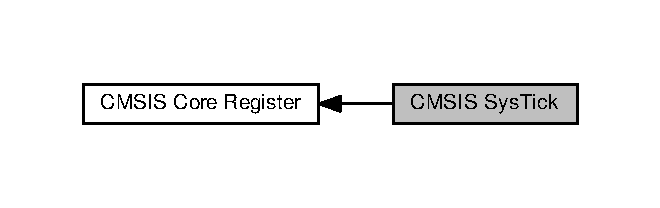
\includegraphics[width=317pt]{group___c_m_s_i_s___sys_tick}
\end{center}
\end{figure}
\subsection*{Classes}
\begin{DoxyCompactItemize}
\item 
struct \hyperlink{struct_sys_tick___type}{Sys\+Tick\+\_\+\+Type}
\begin{DoxyCompactList}\small\item\em Structure type to access the System Timer (Sys\+Tick). \end{DoxyCompactList}\end{DoxyCompactItemize}
\subsection*{Macros}
\begin{DoxyCompactItemize}
\item 
\#define \hyperlink{group___c_m_s_i_s___sys_tick_gadbb65d4a815759649db41df216ed4d60}{Sys\+Tick\+\_\+\+C\+T\+R\+L\+\_\+\+C\+O\+U\+N\+T\+F\+L\+A\+G\+\_\+\+Pos}~16
\item 
\#define \hyperlink{group___c_m_s_i_s___sys_tick_ga1bf3033ecccf200f59baefe15dbb367c}{Sys\+Tick\+\_\+\+C\+T\+R\+L\+\_\+\+C\+O\+U\+N\+T\+F\+L\+A\+G\+\_\+\+Msk}~(1\+U\+L $<$$<$ Sys\+Tick\+\_\+\+C\+T\+R\+L\+\_\+\+C\+O\+U\+N\+T\+F\+L\+A\+G\+\_\+\+Pos)
\item 
\#define \hyperlink{group___c_m_s_i_s___sys_tick_ga24fbc69a5f0b78d67fda2300257baff1}{Sys\+Tick\+\_\+\+C\+T\+R\+L\+\_\+\+C\+L\+K\+S\+O\+U\+R\+C\+E\+\_\+\+Pos}~2
\item 
\#define \hyperlink{group___c_m_s_i_s___sys_tick_gaa41d06039797423a46596bd313d57373}{Sys\+Tick\+\_\+\+C\+T\+R\+L\+\_\+\+C\+L\+K\+S\+O\+U\+R\+C\+E\+\_\+\+Msk}~(1\+U\+L $<$$<$ Sys\+Tick\+\_\+\+C\+T\+R\+L\+\_\+\+C\+L\+K\+S\+O\+U\+R\+C\+E\+\_\+\+Pos)
\item 
\#define \hyperlink{group___c_m_s_i_s___sys_tick_ga88f45bbb89ce8df3cd2b2613c7b48214}{Sys\+Tick\+\_\+\+C\+T\+R\+L\+\_\+\+T\+I\+C\+K\+I\+N\+T\+\_\+\+Pos}~1
\item 
\#define \hyperlink{group___c_m_s_i_s___sys_tick_ga95bb984266ca764024836a870238a027}{Sys\+Tick\+\_\+\+C\+T\+R\+L\+\_\+\+T\+I\+C\+K\+I\+N\+T\+\_\+\+Msk}~(1\+U\+L $<$$<$ Sys\+Tick\+\_\+\+C\+T\+R\+L\+\_\+\+T\+I\+C\+K\+I\+N\+T\+\_\+\+Pos)
\item 
\#define \hyperlink{group___c_m_s_i_s___sys_tick_ga0b48cc1e36d92a92e4bf632890314810}{Sys\+Tick\+\_\+\+C\+T\+R\+L\+\_\+\+E\+N\+A\+B\+L\+E\+\_\+\+Pos}~0
\item 
\#define \hyperlink{group___c_m_s_i_s___sys_tick_ga16c9fee0ed0235524bdeb38af328fd1f}{Sys\+Tick\+\_\+\+C\+T\+R\+L\+\_\+\+E\+N\+A\+B\+L\+E\+\_\+\+Msk}~(1\+U\+L $<$$<$ Sys\+Tick\+\_\+\+C\+T\+R\+L\+\_\+\+E\+N\+A\+B\+L\+E\+\_\+\+Pos)
\item 
\#define \hyperlink{group___c_m_s_i_s___sys_tick_gaf44d10df359dc5bf5752b0894ae3bad2}{Sys\+Tick\+\_\+\+L\+O\+A\+D\+\_\+\+R\+E\+L\+O\+A\+D\+\_\+\+Pos}~0
\item 
\#define \hyperlink{group___c_m_s_i_s___sys_tick_ga265912a7962f0e1abd170336e579b1b1}{Sys\+Tick\+\_\+\+L\+O\+A\+D\+\_\+\+R\+E\+L\+O\+A\+D\+\_\+\+Msk}~(0x\+F\+F\+F\+F\+F\+F\+U\+L $<$$<$ Sys\+Tick\+\_\+\+L\+O\+A\+D\+\_\+\+R\+E\+L\+O\+A\+D\+\_\+\+Pos)
\item 
\#define \hyperlink{group___c_m_s_i_s___sys_tick_ga3208104c3b019b5de35ae8c21d5c34dd}{Sys\+Tick\+\_\+\+V\+A\+L\+\_\+\+C\+U\+R\+R\+E\+N\+T\+\_\+\+Pos}~0
\item 
\#define \hyperlink{group___c_m_s_i_s___sys_tick_gafc77b56d568930b49a2474debc75ab45}{Sys\+Tick\+\_\+\+V\+A\+L\+\_\+\+C\+U\+R\+R\+E\+N\+T\+\_\+\+Msk}~(0x\+F\+F\+F\+F\+F\+F\+U\+L $<$$<$ Sys\+Tick\+\_\+\+V\+A\+L\+\_\+\+C\+U\+R\+R\+E\+N\+T\+\_\+\+Pos)
\item 
\#define \hyperlink{group___c_m_s_i_s___sys_tick_ga534dbe414e7a46a6ce4c1eca1fbff409}{Sys\+Tick\+\_\+\+C\+A\+L\+I\+B\+\_\+\+N\+O\+R\+E\+F\+\_\+\+Pos}~31
\item 
\#define \hyperlink{group___c_m_s_i_s___sys_tick_ga3af0d891fdd99bcc8d8912d37830edb6}{Sys\+Tick\+\_\+\+C\+A\+L\+I\+B\+\_\+\+N\+O\+R\+E\+F\+\_\+\+Msk}~(1\+U\+L $<$$<$ Sys\+Tick\+\_\+\+C\+A\+L\+I\+B\+\_\+\+N\+O\+R\+E\+F\+\_\+\+Pos)
\item 
\#define \hyperlink{group___c_m_s_i_s___sys_tick_gadd0c9cd6641b9f6a0c618e7982954860}{Sys\+Tick\+\_\+\+C\+A\+L\+I\+B\+\_\+\+S\+K\+E\+W\+\_\+\+Pos}~30
\item 
\#define \hyperlink{group___c_m_s_i_s___sys_tick_ga8a6a85a87334776f33d77fd147587431}{Sys\+Tick\+\_\+\+C\+A\+L\+I\+B\+\_\+\+S\+K\+E\+W\+\_\+\+Msk}~(1\+U\+L $<$$<$ Sys\+Tick\+\_\+\+C\+A\+L\+I\+B\+\_\+\+S\+K\+E\+W\+\_\+\+Pos)
\item 
\#define \hyperlink{group___c_m_s_i_s___sys_tick_gacae558f6e75a0bed5d826f606d8e695e}{Sys\+Tick\+\_\+\+C\+A\+L\+I\+B\+\_\+\+T\+E\+N\+M\+S\+\_\+\+Pos}~0
\item 
\#define \hyperlink{group___c_m_s_i_s___sys_tick_gaf1e68865c5aece2ad58971225bd3e95e}{Sys\+Tick\+\_\+\+C\+A\+L\+I\+B\+\_\+\+T\+E\+N\+M\+S\+\_\+\+Msk}~(0x\+F\+F\+F\+F\+F\+F\+U\+L $<$$<$ Sys\+Tick\+\_\+\+V\+A\+L\+\_\+\+C\+U\+R\+R\+E\+N\+T\+\_\+\+Pos)
\end{DoxyCompactItemize}


\subsection{Detailed Description}
Type definitions for the Cortex-\/M System Timer Registers 

\subsection{Macro Definition Documentation}
\index{C\+M\+S\+I\+S Sys\+Tick@{C\+M\+S\+I\+S Sys\+Tick}!Sys\+Tick\+\_\+\+C\+A\+L\+I\+B\+\_\+\+N\+O\+R\+E\+F\+\_\+\+Msk@{Sys\+Tick\+\_\+\+C\+A\+L\+I\+B\+\_\+\+N\+O\+R\+E\+F\+\_\+\+Msk}}
\index{Sys\+Tick\+\_\+\+C\+A\+L\+I\+B\+\_\+\+N\+O\+R\+E\+F\+\_\+\+Msk@{Sys\+Tick\+\_\+\+C\+A\+L\+I\+B\+\_\+\+N\+O\+R\+E\+F\+\_\+\+Msk}!C\+M\+S\+I\+S Sys\+Tick@{C\+M\+S\+I\+S Sys\+Tick}}
\subsubsection[{\texorpdfstring{Sys\+Tick\+\_\+\+C\+A\+L\+I\+B\+\_\+\+N\+O\+R\+E\+F\+\_\+\+Msk}{SysTick_CALIB_NOREF_Msk}}]{\setlength{\rightskip}{0pt plus 5cm}\#define Sys\+Tick\+\_\+\+C\+A\+L\+I\+B\+\_\+\+N\+O\+R\+E\+F\+\_\+\+Msk~(1\+U\+L $<$$<$ Sys\+Tick\+\_\+\+C\+A\+L\+I\+B\+\_\+\+N\+O\+R\+E\+F\+\_\+\+Pos)}\hypertarget{group___c_m_s_i_s___sys_tick_ga3af0d891fdd99bcc8d8912d37830edb6}{}\label{group___c_m_s_i_s___sys_tick_ga3af0d891fdd99bcc8d8912d37830edb6}
Sys\+Tick C\+A\+L\+IB\+: N\+O\+R\+EF Mask 

Definition at line 390 of file core\+\_\+cm0.\+h.

\index{C\+M\+S\+I\+S Sys\+Tick@{C\+M\+S\+I\+S Sys\+Tick}!Sys\+Tick\+\_\+\+C\+A\+L\+I\+B\+\_\+\+N\+O\+R\+E\+F\+\_\+\+Pos@{Sys\+Tick\+\_\+\+C\+A\+L\+I\+B\+\_\+\+N\+O\+R\+E\+F\+\_\+\+Pos}}
\index{Sys\+Tick\+\_\+\+C\+A\+L\+I\+B\+\_\+\+N\+O\+R\+E\+F\+\_\+\+Pos@{Sys\+Tick\+\_\+\+C\+A\+L\+I\+B\+\_\+\+N\+O\+R\+E\+F\+\_\+\+Pos}!C\+M\+S\+I\+S Sys\+Tick@{C\+M\+S\+I\+S Sys\+Tick}}
\subsubsection[{\texorpdfstring{Sys\+Tick\+\_\+\+C\+A\+L\+I\+B\+\_\+\+N\+O\+R\+E\+F\+\_\+\+Pos}{SysTick_CALIB_NOREF_Pos}}]{\setlength{\rightskip}{0pt plus 5cm}\#define Sys\+Tick\+\_\+\+C\+A\+L\+I\+B\+\_\+\+N\+O\+R\+E\+F\+\_\+\+Pos~31}\hypertarget{group___c_m_s_i_s___sys_tick_ga534dbe414e7a46a6ce4c1eca1fbff409}{}\label{group___c_m_s_i_s___sys_tick_ga534dbe414e7a46a6ce4c1eca1fbff409}
Sys\+Tick C\+A\+L\+IB\+: N\+O\+R\+EF Position 

Definition at line 389 of file core\+\_\+cm0.\+h.

\index{C\+M\+S\+I\+S Sys\+Tick@{C\+M\+S\+I\+S Sys\+Tick}!Sys\+Tick\+\_\+\+C\+A\+L\+I\+B\+\_\+\+S\+K\+E\+W\+\_\+\+Msk@{Sys\+Tick\+\_\+\+C\+A\+L\+I\+B\+\_\+\+S\+K\+E\+W\+\_\+\+Msk}}
\index{Sys\+Tick\+\_\+\+C\+A\+L\+I\+B\+\_\+\+S\+K\+E\+W\+\_\+\+Msk@{Sys\+Tick\+\_\+\+C\+A\+L\+I\+B\+\_\+\+S\+K\+E\+W\+\_\+\+Msk}!C\+M\+S\+I\+S Sys\+Tick@{C\+M\+S\+I\+S Sys\+Tick}}
\subsubsection[{\texorpdfstring{Sys\+Tick\+\_\+\+C\+A\+L\+I\+B\+\_\+\+S\+K\+E\+W\+\_\+\+Msk}{SysTick_CALIB_SKEW_Msk}}]{\setlength{\rightskip}{0pt plus 5cm}\#define Sys\+Tick\+\_\+\+C\+A\+L\+I\+B\+\_\+\+S\+K\+E\+W\+\_\+\+Msk~(1\+U\+L $<$$<$ Sys\+Tick\+\_\+\+C\+A\+L\+I\+B\+\_\+\+S\+K\+E\+W\+\_\+\+Pos)}\hypertarget{group___c_m_s_i_s___sys_tick_ga8a6a85a87334776f33d77fd147587431}{}\label{group___c_m_s_i_s___sys_tick_ga8a6a85a87334776f33d77fd147587431}
Sys\+Tick C\+A\+L\+IB\+: S\+K\+EW Mask 

Definition at line 393 of file core\+\_\+cm0.\+h.

\index{C\+M\+S\+I\+S Sys\+Tick@{C\+M\+S\+I\+S Sys\+Tick}!Sys\+Tick\+\_\+\+C\+A\+L\+I\+B\+\_\+\+S\+K\+E\+W\+\_\+\+Pos@{Sys\+Tick\+\_\+\+C\+A\+L\+I\+B\+\_\+\+S\+K\+E\+W\+\_\+\+Pos}}
\index{Sys\+Tick\+\_\+\+C\+A\+L\+I\+B\+\_\+\+S\+K\+E\+W\+\_\+\+Pos@{Sys\+Tick\+\_\+\+C\+A\+L\+I\+B\+\_\+\+S\+K\+E\+W\+\_\+\+Pos}!C\+M\+S\+I\+S Sys\+Tick@{C\+M\+S\+I\+S Sys\+Tick}}
\subsubsection[{\texorpdfstring{Sys\+Tick\+\_\+\+C\+A\+L\+I\+B\+\_\+\+S\+K\+E\+W\+\_\+\+Pos}{SysTick_CALIB_SKEW_Pos}}]{\setlength{\rightskip}{0pt plus 5cm}\#define Sys\+Tick\+\_\+\+C\+A\+L\+I\+B\+\_\+\+S\+K\+E\+W\+\_\+\+Pos~30}\hypertarget{group___c_m_s_i_s___sys_tick_gadd0c9cd6641b9f6a0c618e7982954860}{}\label{group___c_m_s_i_s___sys_tick_gadd0c9cd6641b9f6a0c618e7982954860}
Sys\+Tick C\+A\+L\+IB\+: S\+K\+EW Position 

Definition at line 392 of file core\+\_\+cm0.\+h.

\index{C\+M\+S\+I\+S Sys\+Tick@{C\+M\+S\+I\+S Sys\+Tick}!Sys\+Tick\+\_\+\+C\+A\+L\+I\+B\+\_\+\+T\+E\+N\+M\+S\+\_\+\+Msk@{Sys\+Tick\+\_\+\+C\+A\+L\+I\+B\+\_\+\+T\+E\+N\+M\+S\+\_\+\+Msk}}
\index{Sys\+Tick\+\_\+\+C\+A\+L\+I\+B\+\_\+\+T\+E\+N\+M\+S\+\_\+\+Msk@{Sys\+Tick\+\_\+\+C\+A\+L\+I\+B\+\_\+\+T\+E\+N\+M\+S\+\_\+\+Msk}!C\+M\+S\+I\+S Sys\+Tick@{C\+M\+S\+I\+S Sys\+Tick}}
\subsubsection[{\texorpdfstring{Sys\+Tick\+\_\+\+C\+A\+L\+I\+B\+\_\+\+T\+E\+N\+M\+S\+\_\+\+Msk}{SysTick_CALIB_TENMS_Msk}}]{\setlength{\rightskip}{0pt plus 5cm}\#define Sys\+Tick\+\_\+\+C\+A\+L\+I\+B\+\_\+\+T\+E\+N\+M\+S\+\_\+\+Msk~(0x\+F\+F\+F\+F\+F\+F\+U\+L $<$$<$ Sys\+Tick\+\_\+\+V\+A\+L\+\_\+\+C\+U\+R\+R\+E\+N\+T\+\_\+\+Pos)}\hypertarget{group___c_m_s_i_s___sys_tick_gaf1e68865c5aece2ad58971225bd3e95e}{}\label{group___c_m_s_i_s___sys_tick_gaf1e68865c5aece2ad58971225bd3e95e}
Sys\+Tick C\+A\+L\+IB\+: T\+E\+N\+MS Mask 

Definition at line 396 of file core\+\_\+cm0.\+h.

\index{C\+M\+S\+I\+S Sys\+Tick@{C\+M\+S\+I\+S Sys\+Tick}!Sys\+Tick\+\_\+\+C\+A\+L\+I\+B\+\_\+\+T\+E\+N\+M\+S\+\_\+\+Pos@{Sys\+Tick\+\_\+\+C\+A\+L\+I\+B\+\_\+\+T\+E\+N\+M\+S\+\_\+\+Pos}}
\index{Sys\+Tick\+\_\+\+C\+A\+L\+I\+B\+\_\+\+T\+E\+N\+M\+S\+\_\+\+Pos@{Sys\+Tick\+\_\+\+C\+A\+L\+I\+B\+\_\+\+T\+E\+N\+M\+S\+\_\+\+Pos}!C\+M\+S\+I\+S Sys\+Tick@{C\+M\+S\+I\+S Sys\+Tick}}
\subsubsection[{\texorpdfstring{Sys\+Tick\+\_\+\+C\+A\+L\+I\+B\+\_\+\+T\+E\+N\+M\+S\+\_\+\+Pos}{SysTick_CALIB_TENMS_Pos}}]{\setlength{\rightskip}{0pt plus 5cm}\#define Sys\+Tick\+\_\+\+C\+A\+L\+I\+B\+\_\+\+T\+E\+N\+M\+S\+\_\+\+Pos~0}\hypertarget{group___c_m_s_i_s___sys_tick_gacae558f6e75a0bed5d826f606d8e695e}{}\label{group___c_m_s_i_s___sys_tick_gacae558f6e75a0bed5d826f606d8e695e}
Sys\+Tick C\+A\+L\+IB\+: T\+E\+N\+MS Position 

Definition at line 395 of file core\+\_\+cm0.\+h.

\index{C\+M\+S\+I\+S Sys\+Tick@{C\+M\+S\+I\+S Sys\+Tick}!Sys\+Tick\+\_\+\+C\+T\+R\+L\+\_\+\+C\+L\+K\+S\+O\+U\+R\+C\+E\+\_\+\+Msk@{Sys\+Tick\+\_\+\+C\+T\+R\+L\+\_\+\+C\+L\+K\+S\+O\+U\+R\+C\+E\+\_\+\+Msk}}
\index{Sys\+Tick\+\_\+\+C\+T\+R\+L\+\_\+\+C\+L\+K\+S\+O\+U\+R\+C\+E\+\_\+\+Msk@{Sys\+Tick\+\_\+\+C\+T\+R\+L\+\_\+\+C\+L\+K\+S\+O\+U\+R\+C\+E\+\_\+\+Msk}!C\+M\+S\+I\+S Sys\+Tick@{C\+M\+S\+I\+S Sys\+Tick}}
\subsubsection[{\texorpdfstring{Sys\+Tick\+\_\+\+C\+T\+R\+L\+\_\+\+C\+L\+K\+S\+O\+U\+R\+C\+E\+\_\+\+Msk}{SysTick_CTRL_CLKSOURCE_Msk}}]{\setlength{\rightskip}{0pt plus 5cm}\#define Sys\+Tick\+\_\+\+C\+T\+R\+L\+\_\+\+C\+L\+K\+S\+O\+U\+R\+C\+E\+\_\+\+Msk~(1\+U\+L $<$$<$ Sys\+Tick\+\_\+\+C\+T\+R\+L\+\_\+\+C\+L\+K\+S\+O\+U\+R\+C\+E\+\_\+\+Pos)}\hypertarget{group___c_m_s_i_s___sys_tick_gaa41d06039797423a46596bd313d57373}{}\label{group___c_m_s_i_s___sys_tick_gaa41d06039797423a46596bd313d57373}
Sys\+Tick C\+T\+RL\+: C\+L\+K\+S\+O\+U\+R\+CE Mask 

Definition at line 372 of file core\+\_\+cm0.\+h.

\index{C\+M\+S\+I\+S Sys\+Tick@{C\+M\+S\+I\+S Sys\+Tick}!Sys\+Tick\+\_\+\+C\+T\+R\+L\+\_\+\+C\+L\+K\+S\+O\+U\+R\+C\+E\+\_\+\+Pos@{Sys\+Tick\+\_\+\+C\+T\+R\+L\+\_\+\+C\+L\+K\+S\+O\+U\+R\+C\+E\+\_\+\+Pos}}
\index{Sys\+Tick\+\_\+\+C\+T\+R\+L\+\_\+\+C\+L\+K\+S\+O\+U\+R\+C\+E\+\_\+\+Pos@{Sys\+Tick\+\_\+\+C\+T\+R\+L\+\_\+\+C\+L\+K\+S\+O\+U\+R\+C\+E\+\_\+\+Pos}!C\+M\+S\+I\+S Sys\+Tick@{C\+M\+S\+I\+S Sys\+Tick}}
\subsubsection[{\texorpdfstring{Sys\+Tick\+\_\+\+C\+T\+R\+L\+\_\+\+C\+L\+K\+S\+O\+U\+R\+C\+E\+\_\+\+Pos}{SysTick_CTRL_CLKSOURCE_Pos}}]{\setlength{\rightskip}{0pt plus 5cm}\#define Sys\+Tick\+\_\+\+C\+T\+R\+L\+\_\+\+C\+L\+K\+S\+O\+U\+R\+C\+E\+\_\+\+Pos~2}\hypertarget{group___c_m_s_i_s___sys_tick_ga24fbc69a5f0b78d67fda2300257baff1}{}\label{group___c_m_s_i_s___sys_tick_ga24fbc69a5f0b78d67fda2300257baff1}
Sys\+Tick C\+T\+RL\+: C\+L\+K\+S\+O\+U\+R\+CE Position 

Definition at line 371 of file core\+\_\+cm0.\+h.

\index{C\+M\+S\+I\+S Sys\+Tick@{C\+M\+S\+I\+S Sys\+Tick}!Sys\+Tick\+\_\+\+C\+T\+R\+L\+\_\+\+C\+O\+U\+N\+T\+F\+L\+A\+G\+\_\+\+Msk@{Sys\+Tick\+\_\+\+C\+T\+R\+L\+\_\+\+C\+O\+U\+N\+T\+F\+L\+A\+G\+\_\+\+Msk}}
\index{Sys\+Tick\+\_\+\+C\+T\+R\+L\+\_\+\+C\+O\+U\+N\+T\+F\+L\+A\+G\+\_\+\+Msk@{Sys\+Tick\+\_\+\+C\+T\+R\+L\+\_\+\+C\+O\+U\+N\+T\+F\+L\+A\+G\+\_\+\+Msk}!C\+M\+S\+I\+S Sys\+Tick@{C\+M\+S\+I\+S Sys\+Tick}}
\subsubsection[{\texorpdfstring{Sys\+Tick\+\_\+\+C\+T\+R\+L\+\_\+\+C\+O\+U\+N\+T\+F\+L\+A\+G\+\_\+\+Msk}{SysTick_CTRL_COUNTFLAG_Msk}}]{\setlength{\rightskip}{0pt plus 5cm}\#define Sys\+Tick\+\_\+\+C\+T\+R\+L\+\_\+\+C\+O\+U\+N\+T\+F\+L\+A\+G\+\_\+\+Msk~(1\+U\+L $<$$<$ Sys\+Tick\+\_\+\+C\+T\+R\+L\+\_\+\+C\+O\+U\+N\+T\+F\+L\+A\+G\+\_\+\+Pos)}\hypertarget{group___c_m_s_i_s___sys_tick_ga1bf3033ecccf200f59baefe15dbb367c}{}\label{group___c_m_s_i_s___sys_tick_ga1bf3033ecccf200f59baefe15dbb367c}
Sys\+Tick C\+T\+RL\+: C\+O\+U\+N\+T\+F\+L\+AG Mask 

Definition at line 369 of file core\+\_\+cm0.\+h.

\index{C\+M\+S\+I\+S Sys\+Tick@{C\+M\+S\+I\+S Sys\+Tick}!Sys\+Tick\+\_\+\+C\+T\+R\+L\+\_\+\+C\+O\+U\+N\+T\+F\+L\+A\+G\+\_\+\+Pos@{Sys\+Tick\+\_\+\+C\+T\+R\+L\+\_\+\+C\+O\+U\+N\+T\+F\+L\+A\+G\+\_\+\+Pos}}
\index{Sys\+Tick\+\_\+\+C\+T\+R\+L\+\_\+\+C\+O\+U\+N\+T\+F\+L\+A\+G\+\_\+\+Pos@{Sys\+Tick\+\_\+\+C\+T\+R\+L\+\_\+\+C\+O\+U\+N\+T\+F\+L\+A\+G\+\_\+\+Pos}!C\+M\+S\+I\+S Sys\+Tick@{C\+M\+S\+I\+S Sys\+Tick}}
\subsubsection[{\texorpdfstring{Sys\+Tick\+\_\+\+C\+T\+R\+L\+\_\+\+C\+O\+U\+N\+T\+F\+L\+A\+G\+\_\+\+Pos}{SysTick_CTRL_COUNTFLAG_Pos}}]{\setlength{\rightskip}{0pt plus 5cm}\#define Sys\+Tick\+\_\+\+C\+T\+R\+L\+\_\+\+C\+O\+U\+N\+T\+F\+L\+A\+G\+\_\+\+Pos~16}\hypertarget{group___c_m_s_i_s___sys_tick_gadbb65d4a815759649db41df216ed4d60}{}\label{group___c_m_s_i_s___sys_tick_gadbb65d4a815759649db41df216ed4d60}
Sys\+Tick C\+T\+RL\+: C\+O\+U\+N\+T\+F\+L\+AG Position 

Definition at line 368 of file core\+\_\+cm0.\+h.

\index{C\+M\+S\+I\+S Sys\+Tick@{C\+M\+S\+I\+S Sys\+Tick}!Sys\+Tick\+\_\+\+C\+T\+R\+L\+\_\+\+E\+N\+A\+B\+L\+E\+\_\+\+Msk@{Sys\+Tick\+\_\+\+C\+T\+R\+L\+\_\+\+E\+N\+A\+B\+L\+E\+\_\+\+Msk}}
\index{Sys\+Tick\+\_\+\+C\+T\+R\+L\+\_\+\+E\+N\+A\+B\+L\+E\+\_\+\+Msk@{Sys\+Tick\+\_\+\+C\+T\+R\+L\+\_\+\+E\+N\+A\+B\+L\+E\+\_\+\+Msk}!C\+M\+S\+I\+S Sys\+Tick@{C\+M\+S\+I\+S Sys\+Tick}}
\subsubsection[{\texorpdfstring{Sys\+Tick\+\_\+\+C\+T\+R\+L\+\_\+\+E\+N\+A\+B\+L\+E\+\_\+\+Msk}{SysTick_CTRL_ENABLE_Msk}}]{\setlength{\rightskip}{0pt plus 5cm}\#define Sys\+Tick\+\_\+\+C\+T\+R\+L\+\_\+\+E\+N\+A\+B\+L\+E\+\_\+\+Msk~(1\+U\+L $<$$<$ Sys\+Tick\+\_\+\+C\+T\+R\+L\+\_\+\+E\+N\+A\+B\+L\+E\+\_\+\+Pos)}\hypertarget{group___c_m_s_i_s___sys_tick_ga16c9fee0ed0235524bdeb38af328fd1f}{}\label{group___c_m_s_i_s___sys_tick_ga16c9fee0ed0235524bdeb38af328fd1f}
Sys\+Tick C\+T\+RL\+: E\+N\+A\+B\+LE Mask 

Definition at line 378 of file core\+\_\+cm0.\+h.

\index{C\+M\+S\+I\+S Sys\+Tick@{C\+M\+S\+I\+S Sys\+Tick}!Sys\+Tick\+\_\+\+C\+T\+R\+L\+\_\+\+E\+N\+A\+B\+L\+E\+\_\+\+Pos@{Sys\+Tick\+\_\+\+C\+T\+R\+L\+\_\+\+E\+N\+A\+B\+L\+E\+\_\+\+Pos}}
\index{Sys\+Tick\+\_\+\+C\+T\+R\+L\+\_\+\+E\+N\+A\+B\+L\+E\+\_\+\+Pos@{Sys\+Tick\+\_\+\+C\+T\+R\+L\+\_\+\+E\+N\+A\+B\+L\+E\+\_\+\+Pos}!C\+M\+S\+I\+S Sys\+Tick@{C\+M\+S\+I\+S Sys\+Tick}}
\subsubsection[{\texorpdfstring{Sys\+Tick\+\_\+\+C\+T\+R\+L\+\_\+\+E\+N\+A\+B\+L\+E\+\_\+\+Pos}{SysTick_CTRL_ENABLE_Pos}}]{\setlength{\rightskip}{0pt plus 5cm}\#define Sys\+Tick\+\_\+\+C\+T\+R\+L\+\_\+\+E\+N\+A\+B\+L\+E\+\_\+\+Pos~0}\hypertarget{group___c_m_s_i_s___sys_tick_ga0b48cc1e36d92a92e4bf632890314810}{}\label{group___c_m_s_i_s___sys_tick_ga0b48cc1e36d92a92e4bf632890314810}
Sys\+Tick C\+T\+RL\+: E\+N\+A\+B\+LE Position 

Definition at line 377 of file core\+\_\+cm0.\+h.

\index{C\+M\+S\+I\+S Sys\+Tick@{C\+M\+S\+I\+S Sys\+Tick}!Sys\+Tick\+\_\+\+C\+T\+R\+L\+\_\+\+T\+I\+C\+K\+I\+N\+T\+\_\+\+Msk@{Sys\+Tick\+\_\+\+C\+T\+R\+L\+\_\+\+T\+I\+C\+K\+I\+N\+T\+\_\+\+Msk}}
\index{Sys\+Tick\+\_\+\+C\+T\+R\+L\+\_\+\+T\+I\+C\+K\+I\+N\+T\+\_\+\+Msk@{Sys\+Tick\+\_\+\+C\+T\+R\+L\+\_\+\+T\+I\+C\+K\+I\+N\+T\+\_\+\+Msk}!C\+M\+S\+I\+S Sys\+Tick@{C\+M\+S\+I\+S Sys\+Tick}}
\subsubsection[{\texorpdfstring{Sys\+Tick\+\_\+\+C\+T\+R\+L\+\_\+\+T\+I\+C\+K\+I\+N\+T\+\_\+\+Msk}{SysTick_CTRL_TICKINT_Msk}}]{\setlength{\rightskip}{0pt plus 5cm}\#define Sys\+Tick\+\_\+\+C\+T\+R\+L\+\_\+\+T\+I\+C\+K\+I\+N\+T\+\_\+\+Msk~(1\+U\+L $<$$<$ Sys\+Tick\+\_\+\+C\+T\+R\+L\+\_\+\+T\+I\+C\+K\+I\+N\+T\+\_\+\+Pos)}\hypertarget{group___c_m_s_i_s___sys_tick_ga95bb984266ca764024836a870238a027}{}\label{group___c_m_s_i_s___sys_tick_ga95bb984266ca764024836a870238a027}
Sys\+Tick C\+T\+RL\+: T\+I\+C\+K\+I\+NT Mask 

Definition at line 375 of file core\+\_\+cm0.\+h.

\index{C\+M\+S\+I\+S Sys\+Tick@{C\+M\+S\+I\+S Sys\+Tick}!Sys\+Tick\+\_\+\+C\+T\+R\+L\+\_\+\+T\+I\+C\+K\+I\+N\+T\+\_\+\+Pos@{Sys\+Tick\+\_\+\+C\+T\+R\+L\+\_\+\+T\+I\+C\+K\+I\+N\+T\+\_\+\+Pos}}
\index{Sys\+Tick\+\_\+\+C\+T\+R\+L\+\_\+\+T\+I\+C\+K\+I\+N\+T\+\_\+\+Pos@{Sys\+Tick\+\_\+\+C\+T\+R\+L\+\_\+\+T\+I\+C\+K\+I\+N\+T\+\_\+\+Pos}!C\+M\+S\+I\+S Sys\+Tick@{C\+M\+S\+I\+S Sys\+Tick}}
\subsubsection[{\texorpdfstring{Sys\+Tick\+\_\+\+C\+T\+R\+L\+\_\+\+T\+I\+C\+K\+I\+N\+T\+\_\+\+Pos}{SysTick_CTRL_TICKINT_Pos}}]{\setlength{\rightskip}{0pt plus 5cm}\#define Sys\+Tick\+\_\+\+C\+T\+R\+L\+\_\+\+T\+I\+C\+K\+I\+N\+T\+\_\+\+Pos~1}\hypertarget{group___c_m_s_i_s___sys_tick_ga88f45bbb89ce8df3cd2b2613c7b48214}{}\label{group___c_m_s_i_s___sys_tick_ga88f45bbb89ce8df3cd2b2613c7b48214}
Sys\+Tick C\+T\+RL\+: T\+I\+C\+K\+I\+NT Position 

Definition at line 374 of file core\+\_\+cm0.\+h.

\index{C\+M\+S\+I\+S Sys\+Tick@{C\+M\+S\+I\+S Sys\+Tick}!Sys\+Tick\+\_\+\+L\+O\+A\+D\+\_\+\+R\+E\+L\+O\+A\+D\+\_\+\+Msk@{Sys\+Tick\+\_\+\+L\+O\+A\+D\+\_\+\+R\+E\+L\+O\+A\+D\+\_\+\+Msk}}
\index{Sys\+Tick\+\_\+\+L\+O\+A\+D\+\_\+\+R\+E\+L\+O\+A\+D\+\_\+\+Msk@{Sys\+Tick\+\_\+\+L\+O\+A\+D\+\_\+\+R\+E\+L\+O\+A\+D\+\_\+\+Msk}!C\+M\+S\+I\+S Sys\+Tick@{C\+M\+S\+I\+S Sys\+Tick}}
\subsubsection[{\texorpdfstring{Sys\+Tick\+\_\+\+L\+O\+A\+D\+\_\+\+R\+E\+L\+O\+A\+D\+\_\+\+Msk}{SysTick_LOAD_RELOAD_Msk}}]{\setlength{\rightskip}{0pt plus 5cm}\#define Sys\+Tick\+\_\+\+L\+O\+A\+D\+\_\+\+R\+E\+L\+O\+A\+D\+\_\+\+Msk~(0x\+F\+F\+F\+F\+F\+F\+U\+L $<$$<$ Sys\+Tick\+\_\+\+L\+O\+A\+D\+\_\+\+R\+E\+L\+O\+A\+D\+\_\+\+Pos)}\hypertarget{group___c_m_s_i_s___sys_tick_ga265912a7962f0e1abd170336e579b1b1}{}\label{group___c_m_s_i_s___sys_tick_ga265912a7962f0e1abd170336e579b1b1}
Sys\+Tick L\+O\+AD\+: R\+E\+L\+O\+AD Mask 

Definition at line 382 of file core\+\_\+cm0.\+h.

\index{C\+M\+S\+I\+S Sys\+Tick@{C\+M\+S\+I\+S Sys\+Tick}!Sys\+Tick\+\_\+\+L\+O\+A\+D\+\_\+\+R\+E\+L\+O\+A\+D\+\_\+\+Pos@{Sys\+Tick\+\_\+\+L\+O\+A\+D\+\_\+\+R\+E\+L\+O\+A\+D\+\_\+\+Pos}}
\index{Sys\+Tick\+\_\+\+L\+O\+A\+D\+\_\+\+R\+E\+L\+O\+A\+D\+\_\+\+Pos@{Sys\+Tick\+\_\+\+L\+O\+A\+D\+\_\+\+R\+E\+L\+O\+A\+D\+\_\+\+Pos}!C\+M\+S\+I\+S Sys\+Tick@{C\+M\+S\+I\+S Sys\+Tick}}
\subsubsection[{\texorpdfstring{Sys\+Tick\+\_\+\+L\+O\+A\+D\+\_\+\+R\+E\+L\+O\+A\+D\+\_\+\+Pos}{SysTick_LOAD_RELOAD_Pos}}]{\setlength{\rightskip}{0pt plus 5cm}\#define Sys\+Tick\+\_\+\+L\+O\+A\+D\+\_\+\+R\+E\+L\+O\+A\+D\+\_\+\+Pos~0}\hypertarget{group___c_m_s_i_s___sys_tick_gaf44d10df359dc5bf5752b0894ae3bad2}{}\label{group___c_m_s_i_s___sys_tick_gaf44d10df359dc5bf5752b0894ae3bad2}
Sys\+Tick L\+O\+AD\+: R\+E\+L\+O\+AD Position 

Definition at line 381 of file core\+\_\+cm0.\+h.

\index{C\+M\+S\+I\+S Sys\+Tick@{C\+M\+S\+I\+S Sys\+Tick}!Sys\+Tick\+\_\+\+V\+A\+L\+\_\+\+C\+U\+R\+R\+E\+N\+T\+\_\+\+Msk@{Sys\+Tick\+\_\+\+V\+A\+L\+\_\+\+C\+U\+R\+R\+E\+N\+T\+\_\+\+Msk}}
\index{Sys\+Tick\+\_\+\+V\+A\+L\+\_\+\+C\+U\+R\+R\+E\+N\+T\+\_\+\+Msk@{Sys\+Tick\+\_\+\+V\+A\+L\+\_\+\+C\+U\+R\+R\+E\+N\+T\+\_\+\+Msk}!C\+M\+S\+I\+S Sys\+Tick@{C\+M\+S\+I\+S Sys\+Tick}}
\subsubsection[{\texorpdfstring{Sys\+Tick\+\_\+\+V\+A\+L\+\_\+\+C\+U\+R\+R\+E\+N\+T\+\_\+\+Msk}{SysTick_VAL_CURRENT_Msk}}]{\setlength{\rightskip}{0pt plus 5cm}\#define Sys\+Tick\+\_\+\+V\+A\+L\+\_\+\+C\+U\+R\+R\+E\+N\+T\+\_\+\+Msk~(0x\+F\+F\+F\+F\+F\+F\+U\+L $<$$<$ Sys\+Tick\+\_\+\+V\+A\+L\+\_\+\+C\+U\+R\+R\+E\+N\+T\+\_\+\+Pos)}\hypertarget{group___c_m_s_i_s___sys_tick_gafc77b56d568930b49a2474debc75ab45}{}\label{group___c_m_s_i_s___sys_tick_gafc77b56d568930b49a2474debc75ab45}
Sys\+Tick V\+AL\+: C\+U\+R\+R\+E\+NT Mask 

Definition at line 386 of file core\+\_\+cm0.\+h.

\index{C\+M\+S\+I\+S Sys\+Tick@{C\+M\+S\+I\+S Sys\+Tick}!Sys\+Tick\+\_\+\+V\+A\+L\+\_\+\+C\+U\+R\+R\+E\+N\+T\+\_\+\+Pos@{Sys\+Tick\+\_\+\+V\+A\+L\+\_\+\+C\+U\+R\+R\+E\+N\+T\+\_\+\+Pos}}
\index{Sys\+Tick\+\_\+\+V\+A\+L\+\_\+\+C\+U\+R\+R\+E\+N\+T\+\_\+\+Pos@{Sys\+Tick\+\_\+\+V\+A\+L\+\_\+\+C\+U\+R\+R\+E\+N\+T\+\_\+\+Pos}!C\+M\+S\+I\+S Sys\+Tick@{C\+M\+S\+I\+S Sys\+Tick}}
\subsubsection[{\texorpdfstring{Sys\+Tick\+\_\+\+V\+A\+L\+\_\+\+C\+U\+R\+R\+E\+N\+T\+\_\+\+Pos}{SysTick_VAL_CURRENT_Pos}}]{\setlength{\rightskip}{0pt plus 5cm}\#define Sys\+Tick\+\_\+\+V\+A\+L\+\_\+\+C\+U\+R\+R\+E\+N\+T\+\_\+\+Pos~0}\hypertarget{group___c_m_s_i_s___sys_tick_ga3208104c3b019b5de35ae8c21d5c34dd}{}\label{group___c_m_s_i_s___sys_tick_ga3208104c3b019b5de35ae8c21d5c34dd}
Sys\+Tick V\+AL\+: C\+U\+R\+R\+E\+NT Position 

Definition at line 385 of file core\+\_\+cm0.\+h.


\hypertarget{group___c_m_s_i_s___core_debug}{}\section{C\+M\+S\+IS Core Debug}
\label{group___c_m_s_i_s___core_debug}\index{C\+M\+S\+I\+S Core Debug@{C\+M\+S\+I\+S Core Debug}}
Collaboration diagram for C\+M\+S\+IS Core Debug\+:\nopagebreak
\begin{figure}[H]
\begin{center}
\leavevmode
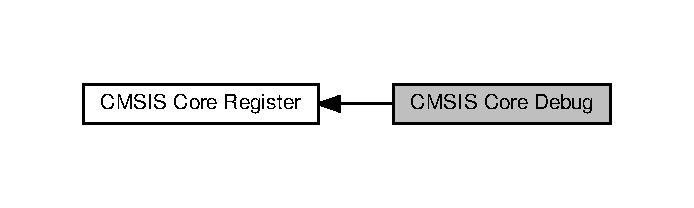
\includegraphics[width=333pt]{group___c_m_s_i_s___core_debug}
\end{center}
\end{figure}
Cortex-\/\+M0 Core Debug Registers (D\+CB registers, S\+H\+C\+SR, and D\+F\+SR) are only accessible over D\+AP and not via processor. Therefore they are not covered by the Cortex-\/\+M0 header file. 
\hypertarget{group___c_m_s_i_s___core___function_interface}{}\section{C\+M\+S\+IS Core Function Interface}
\label{group___c_m_s_i_s___core___function_interface}\index{C\+M\+S\+I\+S Core Function Interface@{C\+M\+S\+I\+S Core Function Interface}}
Collaboration diagram for C\+M\+S\+IS Core Function Interface\+:\nopagebreak
\begin{figure}[H]
\begin{center}
\leavevmode
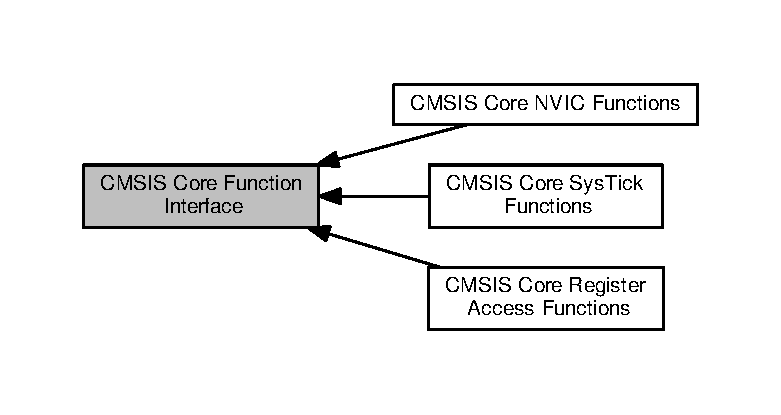
\includegraphics[width=350pt]{group___c_m_s_i_s___core___function_interface}
\end{center}
\end{figure}
\subsection*{Modules}
\begin{DoxyCompactItemize}
\item 
\hyperlink{group___c_m_s_i_s___core___n_v_i_c_functions}{C\+M\+S\+I\+S Core N\+V\+I\+C Functions}
\item 
\hyperlink{group___c_m_s_i_s___core___sys_tick_functions}{C\+M\+S\+I\+S Core Sys\+Tick Functions}
\item 
\hyperlink{group___c_m_s_i_s___core___reg_acc_functions}{C\+M\+S\+I\+S Core Register Access Functions}
\end{DoxyCompactItemize}


\subsection{Detailed Description}
Core Function Interface contains\+:
\begin{DoxyItemize}
\item Core N\+V\+IC Functions
\item Core Sys\+Tick Functions
\item Core Register Access Functions 
\end{DoxyItemize}
\hypertarget{group___c_m_s_i_s___core___n_v_i_c_functions}{}\section{C\+M\+S\+IS Core N\+V\+IC Functions}
\label{group___c_m_s_i_s___core___n_v_i_c_functions}\index{C\+M\+S\+I\+S Core N\+V\+I\+C Functions@{C\+M\+S\+I\+S Core N\+V\+I\+C Functions}}
Collaboration diagram for C\+M\+S\+IS Core N\+V\+IC Functions\+:\nopagebreak
\begin{figure}[H]
\begin{center}
\leavevmode
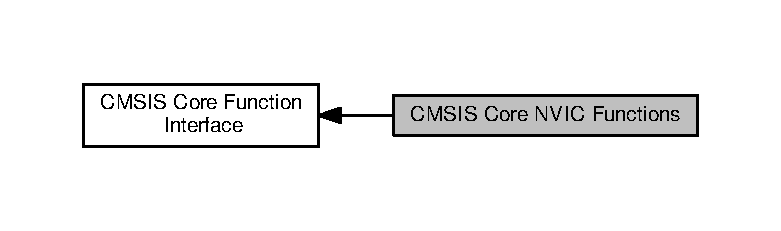
\includegraphics[width=350pt]{group___c_m_s_i_s___core___n_v_i_c_functions}
\end{center}
\end{figure}
\subsection*{Macros}
\begin{DoxyCompactItemize}
\item 
\#define \hyperlink{group___c_m_s_i_s___core___n_v_i_c_functions_ga53c75b28823441c6153269f0ecbed878}{\+\_\+\+B\+I\+T\+\_\+\+S\+H\+I\+FT}(\hyperlink{group___l_p_c11xx___c_m_s_i_s_ga666eb0caeb12ec0e281415592ae89083}{I\+R\+Qn})~(  (((uint32\+\_\+t)(\hyperlink{group___l_p_c11xx___c_m_s_i_s_ga666eb0caeb12ec0e281415592ae89083}{I\+R\+Qn})       )    \&  0x03) $\ast$ 8 )
\item 
\#define \hyperlink{group___c_m_s_i_s___core___n_v_i_c_functions_gaee4f7eb5d7e770ad51489dbceabb1755}{\+\_\+\+S\+H\+P\+\_\+\+I\+DX}(\hyperlink{group___l_p_c11xx___c_m_s_i_s_ga666eb0caeb12ec0e281415592ae89083}{I\+R\+Qn})~( ((((uint32\+\_\+t)(\hyperlink{group___l_p_c11xx___c_m_s_i_s_ga666eb0caeb12ec0e281415592ae89083}{I\+R\+Qn}) \& 0x0\+F)-\/8) $>$$>$    2)     )
\item 
\#define \hyperlink{group___c_m_s_i_s___core___n_v_i_c_functions_ga370ec4b1751a6a889d849747df3763a9}{\+\_\+\+I\+P\+\_\+\+I\+DX}(\hyperlink{group___l_p_c11xx___c_m_s_i_s_ga666eb0caeb12ec0e281415592ae89083}{I\+R\+Qn})~(   ((uint32\+\_\+t)(\hyperlink{group___l_p_c11xx___c_m_s_i_s_ga666eb0caeb12ec0e281415592ae89083}{I\+R\+Qn})            $>$$>$    2)     )
\end{DoxyCompactItemize}


\subsection{Detailed Description}


\subsection{Macro Definition Documentation}
\index{C\+M\+S\+I\+S Core N\+V\+I\+C Functions@{C\+M\+S\+I\+S Core N\+V\+I\+C Functions}!\+\_\+\+B\+I\+T\+\_\+\+S\+H\+I\+FT@{\+\_\+\+B\+I\+T\+\_\+\+S\+H\+I\+FT}}
\index{\+\_\+\+B\+I\+T\+\_\+\+S\+H\+I\+FT@{\+\_\+\+B\+I\+T\+\_\+\+S\+H\+I\+FT}!C\+M\+S\+I\+S Core N\+V\+I\+C Functions@{C\+M\+S\+I\+S Core N\+V\+I\+C Functions}}
\subsubsection[{\texorpdfstring{\+\_\+\+B\+I\+T\+\_\+\+S\+H\+I\+FT}{_BIT_SHIFT}}]{\setlength{\rightskip}{0pt plus 5cm}\#define \+\_\+\+B\+I\+T\+\_\+\+S\+H\+I\+FT(
\begin{DoxyParamCaption}
\item[{}]{{\bf I\+R\+Qn}}
\end{DoxyParamCaption}
)~(  (((uint32\+\_\+t)({\bf I\+R\+Qn})       )    \&  0x03) $\ast$ 8 )}\hypertarget{group___c_m_s_i_s___core___n_v_i_c_functions_ga53c75b28823441c6153269f0ecbed878}{}\label{group___c_m_s_i_s___core___n_v_i_c_functions_ga53c75b28823441c6153269f0ecbed878}


Definition at line 450 of file core\+\_\+cm0.\+h.

\index{C\+M\+S\+I\+S Core N\+V\+I\+C Functions@{C\+M\+S\+I\+S Core N\+V\+I\+C Functions}!\+\_\+\+I\+P\+\_\+\+I\+DX@{\+\_\+\+I\+P\+\_\+\+I\+DX}}
\index{\+\_\+\+I\+P\+\_\+\+I\+DX@{\+\_\+\+I\+P\+\_\+\+I\+DX}!C\+M\+S\+I\+S Core N\+V\+I\+C Functions@{C\+M\+S\+I\+S Core N\+V\+I\+C Functions}}
\subsubsection[{\texorpdfstring{\+\_\+\+I\+P\+\_\+\+I\+DX}{_IP_IDX}}]{\setlength{\rightskip}{0pt plus 5cm}\#define \+\_\+\+I\+P\+\_\+\+I\+DX(
\begin{DoxyParamCaption}
\item[{}]{{\bf I\+R\+Qn}}
\end{DoxyParamCaption}
)~(   ((uint32\+\_\+t)({\bf I\+R\+Qn})            $>$$>$    2)     )}\hypertarget{group___c_m_s_i_s___core___n_v_i_c_functions_ga370ec4b1751a6a889d849747df3763a9}{}\label{group___c_m_s_i_s___core___n_v_i_c_functions_ga370ec4b1751a6a889d849747df3763a9}


Definition at line 452 of file core\+\_\+cm0.\+h.

\index{C\+M\+S\+I\+S Core N\+V\+I\+C Functions@{C\+M\+S\+I\+S Core N\+V\+I\+C Functions}!\+\_\+\+S\+H\+P\+\_\+\+I\+DX@{\+\_\+\+S\+H\+P\+\_\+\+I\+DX}}
\index{\+\_\+\+S\+H\+P\+\_\+\+I\+DX@{\+\_\+\+S\+H\+P\+\_\+\+I\+DX}!C\+M\+S\+I\+S Core N\+V\+I\+C Functions@{C\+M\+S\+I\+S Core N\+V\+I\+C Functions}}
\subsubsection[{\texorpdfstring{\+\_\+\+S\+H\+P\+\_\+\+I\+DX}{_SHP_IDX}}]{\setlength{\rightskip}{0pt plus 5cm}\#define \+\_\+\+S\+H\+P\+\_\+\+I\+DX(
\begin{DoxyParamCaption}
\item[{}]{{\bf I\+R\+Qn}}
\end{DoxyParamCaption}
)~( ((((uint32\+\_\+t)({\bf I\+R\+Qn}) \& 0x0\+F)-\/8) $>$$>$    2)     )}\hypertarget{group___c_m_s_i_s___core___n_v_i_c_functions_gaee4f7eb5d7e770ad51489dbceabb1755}{}\label{group___c_m_s_i_s___core___n_v_i_c_functions_gaee4f7eb5d7e770ad51489dbceabb1755}


Definition at line 451 of file core\+\_\+cm0.\+h.


\hypertarget{group___c_m_s_i_s___core___sys_tick_functions}{}\section{C\+M\+S\+IS Core Sys\+Tick Functions}
\label{group___c_m_s_i_s___core___sys_tick_functions}\index{C\+M\+S\+I\+S Core Sys\+Tick Functions@{C\+M\+S\+I\+S Core Sys\+Tick Functions}}
Collaboration diagram for C\+M\+S\+IS Core Sys\+Tick Functions\+:\nopagebreak
\begin{figure}[H]
\begin{center}
\leavevmode
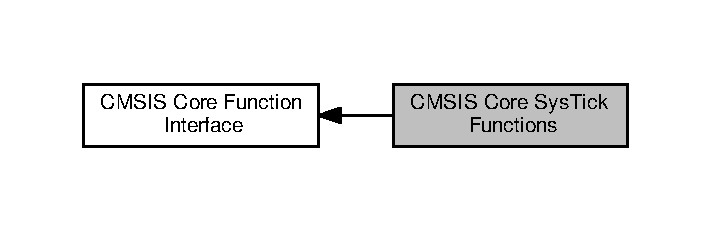
\includegraphics[width=341pt]{group___c_m_s_i_s___core___sys_tick_functions}
\end{center}
\end{figure}


\subsection{Detailed Description}

\hypertarget{group___c_m_s_i_s___core___reg_acc_functions}{}\section{C\+M\+S\+IS Core Register Access Functions}
\label{group___c_m_s_i_s___core___reg_acc_functions}\index{C\+M\+S\+I\+S Core Register Access Functions@{C\+M\+S\+I\+S Core Register Access Functions}}
Collaboration diagram for C\+M\+S\+IS Core Register Access Functions\+:\nopagebreak
\begin{figure}[H]
\begin{center}
\leavevmode
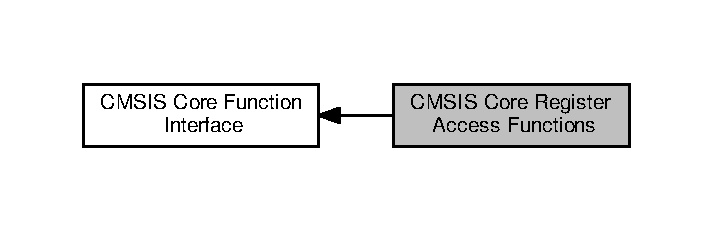
\includegraphics[width=342pt]{group___c_m_s_i_s___core___reg_acc_functions}
\end{center}
\end{figure}

\hypertarget{group___c_m_s_i_s___core___instruction_interface}{}\section{C\+M\+S\+IS Core Instruction Interface}
\label{group___c_m_s_i_s___core___instruction_interface}\index{C\+M\+S\+I\+S Core Instruction Interface@{C\+M\+S\+I\+S Core Instruction Interface}}
Access to dedicated instructions 
\hypertarget{group___l_p_c___i_o_c_o_n___l_p_c1102___d_e_f_i_n_e_s}{}\section{Defines I\+O\+C\+ON L\+P\+C1102}
\label{group___l_p_c___i_o_c_o_n___l_p_c1102___d_e_f_i_n_e_s}\index{Defines I\+O\+C\+O\+N L\+P\+C1102@{Defines I\+O\+C\+O\+N L\+P\+C1102}}


Defines asociados al set de registros I\+O\+C\+ON del L\+P\+C1102.  


Collaboration diagram for Defines I\+O\+C\+ON L\+P\+C1102\+:\nopagebreak
\begin{figure}[H]
\begin{center}
\leavevmode
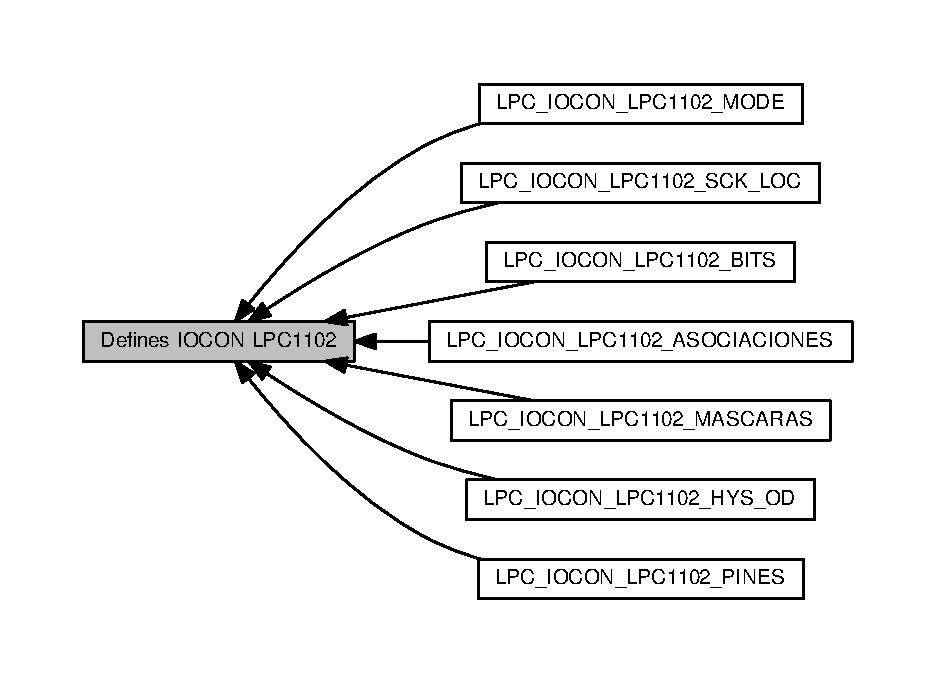
\includegraphics[width=350pt]{group___l_p_c___i_o_c_o_n___l_p_c1102___d_e_f_i_n_e_s}
\end{center}
\end{figure}
\subsection*{Modules}
\begin{DoxyCompactItemize}
\item 
\hyperlink{group___l_p_c___i_o_c_o_n___l_p_c1102___b_i_t_s}{L\+P\+C\+\_\+\+I\+O\+C\+O\+N\+\_\+\+L\+P\+C1102\+\_\+\+B\+I\+TS}
\begin{DoxyCompactList}\small\item\em Bits del registro I\+O\+C\+ON L\+P\+C1102. \end{DoxyCompactList}\item 
\hyperlink{group___l_p_c___i_o_c_o_n___l_p_c1102___m_a_s_c_a_r_a_s}{L\+P\+C\+\_\+\+I\+O\+C\+O\+N\+\_\+\+L\+P\+C1102\+\_\+\+M\+A\+S\+C\+A\+R\+AS}
\begin{DoxyCompactList}\small\item\em Mascaras del registro I\+O\+C\+ON L\+P\+C1102. \end{DoxyCompactList}\item 
\hyperlink{group___l_p_c___i_o_c_o_n___l_p_c1102___p_i_n_e_s}{L\+P\+C\+\_\+\+I\+O\+C\+O\+N\+\_\+\+L\+P\+C1102\+\_\+\+P\+I\+N\+ES}
\begin{DoxyCompactList}\small\item\em Funciones de cada pin asociados a los registros I\+O\+C\+ON. \end{DoxyCompactList}\item 
\hyperlink{group___l_p_c___i_o_c_o_n___l_p_c1102___m_o_d_e}{L\+P\+C\+\_\+\+I\+O\+C\+O\+N\+\_\+\+L\+P\+C1102\+\_\+\+M\+O\+DE}
\begin{DoxyCompactList}\small\item\em Modos del registro I\+O\+C\+ON comunes a todos los pines. \end{DoxyCompactList}\item 
\hyperlink{group___l_p_c___i_o_c_o_n___l_p_c1102___h_y_s___o_d}{L\+P\+C\+\_\+\+I\+O\+C\+O\+N\+\_\+\+L\+P\+C1102\+\_\+\+H\+Y\+S\+\_\+\+OD}
\begin{DoxyCompactList}\small\item\em Bits de histéresis y Open\+Drain. \end{DoxyCompactList}\item 
\hyperlink{group___l_p_c___i_o_c_o_n___l_p_c1102___a_s_o_c_i_a_c_i_o_n_e_s}{L\+P\+C\+\_\+\+I\+O\+C\+O\+N\+\_\+\+L\+P\+C1102\+\_\+\+A\+S\+O\+C\+I\+A\+C\+I\+O\+N\+ES}
\begin{DoxyCompactList}\small\item\em Asociacion del nombre del registro en la estructura L\+P\+C\+\_\+\+I\+O\+C\+ON con los nombres del manual de $<$letra$>$$<$nro$>$ \end{DoxyCompactList}\item 
\hyperlink{group___l_p_c___i_o_c_o_n___l_p_c1102___s_c_k___l_o_c}{L\+P\+C\+\_\+\+I\+O\+C\+O\+N\+\_\+\+L\+P\+C1102\+\_\+\+S\+C\+K\+\_\+\+L\+OC}
\begin{DoxyCompactList}\small\item\em Registro que define en qué pin se asocia la función S\+CK. \end{DoxyCompactList}\end{DoxyCompactItemize}


\subsection{Detailed Description}
Defines asociados al set de registros I\+O\+C\+ON del L\+P\+C1102. 


\hypertarget{group___l_p_c___i_o_c_o_n___l_p_c1102___b_i_t_s}{}\section{L\+P\+C\+\_\+\+I\+O\+C\+O\+N\+\_\+\+L\+P\+C1102\+\_\+\+B\+I\+TS}
\label{group___l_p_c___i_o_c_o_n___l_p_c1102___b_i_t_s}\index{L\+P\+C\+\_\+\+I\+O\+C\+O\+N\+\_\+\+L\+P\+C1102\+\_\+\+B\+I\+TS@{L\+P\+C\+\_\+\+I\+O\+C\+O\+N\+\_\+\+L\+P\+C1102\+\_\+\+B\+I\+TS}}


Bits del registro I\+O\+C\+ON L\+P\+C1102.  


Collaboration diagram for L\+P\+C\+\_\+\+I\+O\+C\+O\+N\+\_\+\+L\+P\+C1102\+\_\+\+B\+I\+TS\+:\nopagebreak
\begin{figure}[H]
\begin{center}
\leavevmode
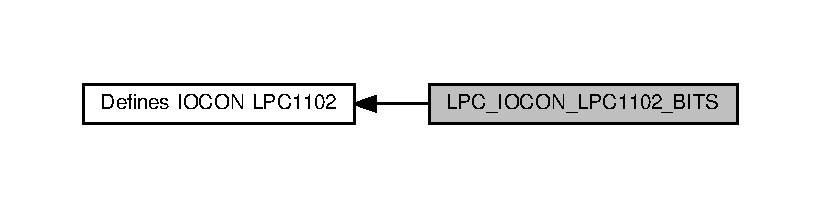
\includegraphics[width=350pt]{group___l_p_c___i_o_c_o_n___l_p_c1102___b_i_t_s}
\end{center}
\end{figure}
\subsection*{Macros}
\begin{DoxyCompactItemize}
\item 
\#define \hyperlink{group___l_p_c___i_o_c_o_n___l_p_c1102___b_i_t_s_ga2d9600555b95756df39218dbb47851ae}{L\+P\+C\+\_\+\+I\+O\+C\+O\+N\+\_\+\+F\+U\+N\+C\+\_\+\+B\+IT}~(0)
\begin{DoxyCompactList}\small\item\em Bit de función. \end{DoxyCompactList}\item 
\#define \hyperlink{group___l_p_c___i_o_c_o_n___l_p_c1102___b_i_t_s_ga793b5ab5e1ab4f784e43a86a2d1ff21f}{L\+P\+C\+\_\+\+I\+O\+C\+O\+N\+\_\+\+M\+O\+D\+E\+\_\+\+B\+IT}~(3)
\begin{DoxyCompactList}\small\item\em Bits de Modo. \end{DoxyCompactList}\item 
\#define \hyperlink{group___l_p_c___i_o_c_o_n___l_p_c1102___b_i_t_s_ga4bdb40fca164c65756bd1c3e69207b62}{L\+P\+C\+\_\+\+I\+O\+C\+O\+N\+\_\+\+H\+Y\+S\+\_\+\+B\+IT}~(5)
\begin{DoxyCompactList}\small\item\em Bit de histeresis. \end{DoxyCompactList}\item 
\#define \hyperlink{group___l_p_c___i_o_c_o_n___l_p_c1102___b_i_t_s_ga0ed826952d05716fdcf3252675de3b93}{L\+P\+C\+\_\+\+I\+O\+C\+O\+N\+\_\+\+A\+D\+M\+O\+D\+E\+\_\+\+B\+IT}~(7)
\begin{DoxyCompactList}\small\item\em Bit de modo analogico o digital. \end{DoxyCompactList}\item 
\#define \hyperlink{group___l_p_c___i_o_c_o_n___l_p_c1102___b_i_t_s_ga62a2b807caf0cfa8371cf1df6f5c9a21}{L\+P\+C\+\_\+\+I\+O\+C\+O\+N\+\_\+\+O\+D\+\_\+\+B\+IT}~(10)
\begin{DoxyCompactList}\small\item\em Bit de Open Drain. \end{DoxyCompactList}\end{DoxyCompactItemize}


\subsection{Detailed Description}
Bits del registro I\+O\+C\+ON L\+P\+C1102. 



\subsection{Macro Definition Documentation}
\index{L\+P\+C\+\_\+\+I\+O\+C\+O\+N\+\_\+\+L\+P\+C1102\+\_\+\+B\+I\+TS@{L\+P\+C\+\_\+\+I\+O\+C\+O\+N\+\_\+\+L\+P\+C1102\+\_\+\+B\+I\+TS}!L\+P\+C\+\_\+\+I\+O\+C\+O\+N\+\_\+\+A\+D\+M\+O\+D\+E\+\_\+\+B\+IT@{L\+P\+C\+\_\+\+I\+O\+C\+O\+N\+\_\+\+A\+D\+M\+O\+D\+E\+\_\+\+B\+IT}}
\index{L\+P\+C\+\_\+\+I\+O\+C\+O\+N\+\_\+\+A\+D\+M\+O\+D\+E\+\_\+\+B\+IT@{L\+P\+C\+\_\+\+I\+O\+C\+O\+N\+\_\+\+A\+D\+M\+O\+D\+E\+\_\+\+B\+IT}!L\+P\+C\+\_\+\+I\+O\+C\+O\+N\+\_\+\+L\+P\+C1102\+\_\+\+B\+I\+TS@{L\+P\+C\+\_\+\+I\+O\+C\+O\+N\+\_\+\+L\+P\+C1102\+\_\+\+B\+I\+TS}}
\subsubsection[{\texorpdfstring{L\+P\+C\+\_\+\+I\+O\+C\+O\+N\+\_\+\+A\+D\+M\+O\+D\+E\+\_\+\+B\+IT}{LPC_IOCON_ADMODE_BIT}}]{\setlength{\rightskip}{0pt plus 5cm}\#define L\+P\+C\+\_\+\+I\+O\+C\+O\+N\+\_\+\+A\+D\+M\+O\+D\+E\+\_\+\+B\+IT~(7)}\hypertarget{group___l_p_c___i_o_c_o_n___l_p_c1102___b_i_t_s_ga0ed826952d05716fdcf3252675de3b93}{}\label{group___l_p_c___i_o_c_o_n___l_p_c1102___b_i_t_s_ga0ed826952d05716fdcf3252675de3b93}


Bit de modo analogico o digital. 



Definition at line 40 of file L\+P\+C1102\+\_\+\+I\+O\+C\+O\+N.\+h.

\index{L\+P\+C\+\_\+\+I\+O\+C\+O\+N\+\_\+\+L\+P\+C1102\+\_\+\+B\+I\+TS@{L\+P\+C\+\_\+\+I\+O\+C\+O\+N\+\_\+\+L\+P\+C1102\+\_\+\+B\+I\+TS}!L\+P\+C\+\_\+\+I\+O\+C\+O\+N\+\_\+\+F\+U\+N\+C\+\_\+\+B\+IT@{L\+P\+C\+\_\+\+I\+O\+C\+O\+N\+\_\+\+F\+U\+N\+C\+\_\+\+B\+IT}}
\index{L\+P\+C\+\_\+\+I\+O\+C\+O\+N\+\_\+\+F\+U\+N\+C\+\_\+\+B\+IT@{L\+P\+C\+\_\+\+I\+O\+C\+O\+N\+\_\+\+F\+U\+N\+C\+\_\+\+B\+IT}!L\+P\+C\+\_\+\+I\+O\+C\+O\+N\+\_\+\+L\+P\+C1102\+\_\+\+B\+I\+TS@{L\+P\+C\+\_\+\+I\+O\+C\+O\+N\+\_\+\+L\+P\+C1102\+\_\+\+B\+I\+TS}}
\subsubsection[{\texorpdfstring{L\+P\+C\+\_\+\+I\+O\+C\+O\+N\+\_\+\+F\+U\+N\+C\+\_\+\+B\+IT}{LPC_IOCON_FUNC_BIT}}]{\setlength{\rightskip}{0pt plus 5cm}\#define L\+P\+C\+\_\+\+I\+O\+C\+O\+N\+\_\+\+F\+U\+N\+C\+\_\+\+B\+IT~(0)}\hypertarget{group___l_p_c___i_o_c_o_n___l_p_c1102___b_i_t_s_ga2d9600555b95756df39218dbb47851ae}{}\label{group___l_p_c___i_o_c_o_n___l_p_c1102___b_i_t_s_ga2d9600555b95756df39218dbb47851ae}


Bit de función. 



Definition at line 34 of file L\+P\+C1102\+\_\+\+I\+O\+C\+O\+N.\+h.

\index{L\+P\+C\+\_\+\+I\+O\+C\+O\+N\+\_\+\+L\+P\+C1102\+\_\+\+B\+I\+TS@{L\+P\+C\+\_\+\+I\+O\+C\+O\+N\+\_\+\+L\+P\+C1102\+\_\+\+B\+I\+TS}!L\+P\+C\+\_\+\+I\+O\+C\+O\+N\+\_\+\+H\+Y\+S\+\_\+\+B\+IT@{L\+P\+C\+\_\+\+I\+O\+C\+O\+N\+\_\+\+H\+Y\+S\+\_\+\+B\+IT}}
\index{L\+P\+C\+\_\+\+I\+O\+C\+O\+N\+\_\+\+H\+Y\+S\+\_\+\+B\+IT@{L\+P\+C\+\_\+\+I\+O\+C\+O\+N\+\_\+\+H\+Y\+S\+\_\+\+B\+IT}!L\+P\+C\+\_\+\+I\+O\+C\+O\+N\+\_\+\+L\+P\+C1102\+\_\+\+B\+I\+TS@{L\+P\+C\+\_\+\+I\+O\+C\+O\+N\+\_\+\+L\+P\+C1102\+\_\+\+B\+I\+TS}}
\subsubsection[{\texorpdfstring{L\+P\+C\+\_\+\+I\+O\+C\+O\+N\+\_\+\+H\+Y\+S\+\_\+\+B\+IT}{LPC_IOCON_HYS_BIT}}]{\setlength{\rightskip}{0pt plus 5cm}\#define L\+P\+C\+\_\+\+I\+O\+C\+O\+N\+\_\+\+H\+Y\+S\+\_\+\+B\+IT~(5)}\hypertarget{group___l_p_c___i_o_c_o_n___l_p_c1102___b_i_t_s_ga4bdb40fca164c65756bd1c3e69207b62}{}\label{group___l_p_c___i_o_c_o_n___l_p_c1102___b_i_t_s_ga4bdb40fca164c65756bd1c3e69207b62}


Bit de histeresis. 



Definition at line 38 of file L\+P\+C1102\+\_\+\+I\+O\+C\+O\+N.\+h.

\index{L\+P\+C\+\_\+\+I\+O\+C\+O\+N\+\_\+\+L\+P\+C1102\+\_\+\+B\+I\+TS@{L\+P\+C\+\_\+\+I\+O\+C\+O\+N\+\_\+\+L\+P\+C1102\+\_\+\+B\+I\+TS}!L\+P\+C\+\_\+\+I\+O\+C\+O\+N\+\_\+\+M\+O\+D\+E\+\_\+\+B\+IT@{L\+P\+C\+\_\+\+I\+O\+C\+O\+N\+\_\+\+M\+O\+D\+E\+\_\+\+B\+IT}}
\index{L\+P\+C\+\_\+\+I\+O\+C\+O\+N\+\_\+\+M\+O\+D\+E\+\_\+\+B\+IT@{L\+P\+C\+\_\+\+I\+O\+C\+O\+N\+\_\+\+M\+O\+D\+E\+\_\+\+B\+IT}!L\+P\+C\+\_\+\+I\+O\+C\+O\+N\+\_\+\+L\+P\+C1102\+\_\+\+B\+I\+TS@{L\+P\+C\+\_\+\+I\+O\+C\+O\+N\+\_\+\+L\+P\+C1102\+\_\+\+B\+I\+TS}}
\subsubsection[{\texorpdfstring{L\+P\+C\+\_\+\+I\+O\+C\+O\+N\+\_\+\+M\+O\+D\+E\+\_\+\+B\+IT}{LPC_IOCON_MODE_BIT}}]{\setlength{\rightskip}{0pt plus 5cm}\#define L\+P\+C\+\_\+\+I\+O\+C\+O\+N\+\_\+\+M\+O\+D\+E\+\_\+\+B\+IT~(3)}\hypertarget{group___l_p_c___i_o_c_o_n___l_p_c1102___b_i_t_s_ga793b5ab5e1ab4f784e43a86a2d1ff21f}{}\label{group___l_p_c___i_o_c_o_n___l_p_c1102___b_i_t_s_ga793b5ab5e1ab4f784e43a86a2d1ff21f}


Bits de Modo. 



Definition at line 36 of file L\+P\+C1102\+\_\+\+I\+O\+C\+O\+N.\+h.

\index{L\+P\+C\+\_\+\+I\+O\+C\+O\+N\+\_\+\+L\+P\+C1102\+\_\+\+B\+I\+TS@{L\+P\+C\+\_\+\+I\+O\+C\+O\+N\+\_\+\+L\+P\+C1102\+\_\+\+B\+I\+TS}!L\+P\+C\+\_\+\+I\+O\+C\+O\+N\+\_\+\+O\+D\+\_\+\+B\+IT@{L\+P\+C\+\_\+\+I\+O\+C\+O\+N\+\_\+\+O\+D\+\_\+\+B\+IT}}
\index{L\+P\+C\+\_\+\+I\+O\+C\+O\+N\+\_\+\+O\+D\+\_\+\+B\+IT@{L\+P\+C\+\_\+\+I\+O\+C\+O\+N\+\_\+\+O\+D\+\_\+\+B\+IT}!L\+P\+C\+\_\+\+I\+O\+C\+O\+N\+\_\+\+L\+P\+C1102\+\_\+\+B\+I\+TS@{L\+P\+C\+\_\+\+I\+O\+C\+O\+N\+\_\+\+L\+P\+C1102\+\_\+\+B\+I\+TS}}
\subsubsection[{\texorpdfstring{L\+P\+C\+\_\+\+I\+O\+C\+O\+N\+\_\+\+O\+D\+\_\+\+B\+IT}{LPC_IOCON_OD_BIT}}]{\setlength{\rightskip}{0pt plus 5cm}\#define L\+P\+C\+\_\+\+I\+O\+C\+O\+N\+\_\+\+O\+D\+\_\+\+B\+IT~(10)}\hypertarget{group___l_p_c___i_o_c_o_n___l_p_c1102___b_i_t_s_ga62a2b807caf0cfa8371cf1df6f5c9a21}{}\label{group___l_p_c___i_o_c_o_n___l_p_c1102___b_i_t_s_ga62a2b807caf0cfa8371cf1df6f5c9a21}


Bit de Open Drain. 



Definition at line 42 of file L\+P\+C1102\+\_\+\+I\+O\+C\+O\+N.\+h.


\hypertarget{group___l_p_c___i_o_c_o_n___l_p_c1102___m_a_s_c_a_r_a_s}{}\section{L\+P\+C\+\_\+\+I\+O\+C\+O\+N\+\_\+\+L\+P\+C1102\+\_\+\+M\+A\+S\+C\+A\+R\+AS}
\label{group___l_p_c___i_o_c_o_n___l_p_c1102___m_a_s_c_a_r_a_s}\index{L\+P\+C\+\_\+\+I\+O\+C\+O\+N\+\_\+\+L\+P\+C1102\+\_\+\+M\+A\+S\+C\+A\+R\+AS@{L\+P\+C\+\_\+\+I\+O\+C\+O\+N\+\_\+\+L\+P\+C1102\+\_\+\+M\+A\+S\+C\+A\+R\+AS}}


Mascaras del registro I\+O\+C\+ON L\+P\+C1102.  


Collaboration diagram for L\+P\+C\+\_\+\+I\+O\+C\+O\+N\+\_\+\+L\+P\+C1102\+\_\+\+M\+A\+S\+C\+A\+R\+AS\+:\nopagebreak
\begin{figure}[H]
\begin{center}
\leavevmode
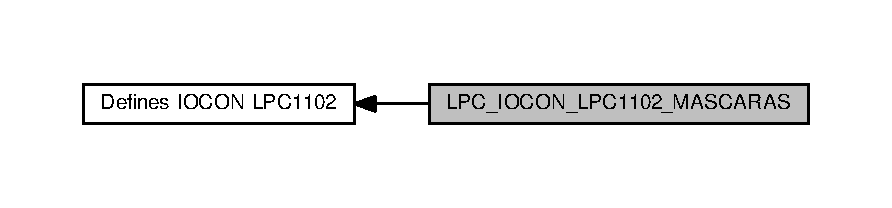
\includegraphics[width=350pt]{group___l_p_c___i_o_c_o_n___l_p_c1102___m_a_s_c_a_r_a_s}
\end{center}
\end{figure}
\subsection*{Macros}
\begin{DoxyCompactItemize}
\item 
\#define \hyperlink{group___l_p_c___i_o_c_o_n___l_p_c1102___m_a_s_c_a_r_a_s_ga429d63df506589f85224d3c12fd61e3b}{L\+P\+C\+\_\+\+I\+O\+C\+O\+N\+\_\+\+F\+U\+N\+C\+\_\+\+M\+AS}~(0x00000007\+U\+L) $<$$<$ L\+P\+C\+\_\+\+I\+O\+C\+O\+N\+\_\+\+F\+U\+N\+C\+\_\+\+B\+IT
\item 
\#define \hyperlink{group___l_p_c___i_o_c_o_n___l_p_c1102___m_a_s_c_a_r_a_s_gac56363757324c51a61e36e9471024b05}{L\+P\+C\+\_\+\+I\+O\+C\+O\+N\+\_\+\+M\+O\+D\+E\+\_\+\+M\+AS}~(0x00000003\+U\+L) $<$$<$ L\+P\+C\+\_\+\+I\+O\+C\+O\+N\+\_\+\+M\+O\+D\+E\+\_\+\+B\+IT
\item 
\#define \hyperlink{group___l_p_c___i_o_c_o_n___l_p_c1102___m_a_s_c_a_r_a_s_ga0f8ccfc34bf41c0deced30305a2d17e5}{L\+P\+C\+\_\+\+I\+O\+C\+O\+N\+\_\+\+H\+Y\+S\+\_\+\+M\+AS}~(0x00000001\+U\+L) $<$$<$ L\+P\+C\+\_\+\+I\+O\+C\+O\+N\+\_\+\+H\+Y\+S\+\_\+\+B\+IT
\item 
\#define \hyperlink{group___l_p_c___i_o_c_o_n___l_p_c1102___m_a_s_c_a_r_a_s_ga63379280f01e70a858b26114f4949794}{L\+P\+C\+\_\+\+I\+O\+C\+O\+N\+\_\+\+O\+D\+\_\+\+M\+AS}~(0x00000001\+U\+L) $<$$<$ L\+P\+C\+\_\+\+I\+O\+C\+O\+N\+\_\+\+O\+D\+\_\+\+B\+IT
\end{DoxyCompactItemize}


\subsection{Detailed Description}
Mascaras del registro I\+O\+C\+ON L\+P\+C1102. 



\subsection{Macro Definition Documentation}
\index{L\+P\+C\+\_\+\+I\+O\+C\+O\+N\+\_\+\+L\+P\+C1102\+\_\+\+M\+A\+S\+C\+A\+R\+AS@{L\+P\+C\+\_\+\+I\+O\+C\+O\+N\+\_\+\+L\+P\+C1102\+\_\+\+M\+A\+S\+C\+A\+R\+AS}!L\+P\+C\+\_\+\+I\+O\+C\+O\+N\+\_\+\+F\+U\+N\+C\+\_\+\+M\+AS@{L\+P\+C\+\_\+\+I\+O\+C\+O\+N\+\_\+\+F\+U\+N\+C\+\_\+\+M\+AS}}
\index{L\+P\+C\+\_\+\+I\+O\+C\+O\+N\+\_\+\+F\+U\+N\+C\+\_\+\+M\+AS@{L\+P\+C\+\_\+\+I\+O\+C\+O\+N\+\_\+\+F\+U\+N\+C\+\_\+\+M\+AS}!L\+P\+C\+\_\+\+I\+O\+C\+O\+N\+\_\+\+L\+P\+C1102\+\_\+\+M\+A\+S\+C\+A\+R\+AS@{L\+P\+C\+\_\+\+I\+O\+C\+O\+N\+\_\+\+L\+P\+C1102\+\_\+\+M\+A\+S\+C\+A\+R\+AS}}
\subsubsection[{\texorpdfstring{L\+P\+C\+\_\+\+I\+O\+C\+O\+N\+\_\+\+F\+U\+N\+C\+\_\+\+M\+AS}{LPC_IOCON_FUNC_MAS}}]{\setlength{\rightskip}{0pt plus 5cm}\#define L\+P\+C\+\_\+\+I\+O\+C\+O\+N\+\_\+\+F\+U\+N\+C\+\_\+\+M\+AS~(0x00000007\+U\+L) $<$$<$ L\+P\+C\+\_\+\+I\+O\+C\+O\+N\+\_\+\+F\+U\+N\+C\+\_\+\+B\+IT}\hypertarget{group___l_p_c___i_o_c_o_n___l_p_c1102___m_a_s_c_a_r_a_s_ga429d63df506589f85224d3c12fd61e3b}{}\label{group___l_p_c___i_o_c_o_n___l_p_c1102___m_a_s_c_a_r_a_s_ga429d63df506589f85224d3c12fd61e3b}
Mascara de bits de función 

Definition at line 55 of file L\+P\+C1102\+\_\+\+I\+O\+C\+O\+N.\+h.

\index{L\+P\+C\+\_\+\+I\+O\+C\+O\+N\+\_\+\+L\+P\+C1102\+\_\+\+M\+A\+S\+C\+A\+R\+AS@{L\+P\+C\+\_\+\+I\+O\+C\+O\+N\+\_\+\+L\+P\+C1102\+\_\+\+M\+A\+S\+C\+A\+R\+AS}!L\+P\+C\+\_\+\+I\+O\+C\+O\+N\+\_\+\+H\+Y\+S\+\_\+\+M\+AS@{L\+P\+C\+\_\+\+I\+O\+C\+O\+N\+\_\+\+H\+Y\+S\+\_\+\+M\+AS}}
\index{L\+P\+C\+\_\+\+I\+O\+C\+O\+N\+\_\+\+H\+Y\+S\+\_\+\+M\+AS@{L\+P\+C\+\_\+\+I\+O\+C\+O\+N\+\_\+\+H\+Y\+S\+\_\+\+M\+AS}!L\+P\+C\+\_\+\+I\+O\+C\+O\+N\+\_\+\+L\+P\+C1102\+\_\+\+M\+A\+S\+C\+A\+R\+AS@{L\+P\+C\+\_\+\+I\+O\+C\+O\+N\+\_\+\+L\+P\+C1102\+\_\+\+M\+A\+S\+C\+A\+R\+AS}}
\subsubsection[{\texorpdfstring{L\+P\+C\+\_\+\+I\+O\+C\+O\+N\+\_\+\+H\+Y\+S\+\_\+\+M\+AS}{LPC_IOCON_HYS_MAS}}]{\setlength{\rightskip}{0pt plus 5cm}\#define L\+P\+C\+\_\+\+I\+O\+C\+O\+N\+\_\+\+H\+Y\+S\+\_\+\+M\+AS~(0x00000001\+U\+L) $<$$<$ L\+P\+C\+\_\+\+I\+O\+C\+O\+N\+\_\+\+H\+Y\+S\+\_\+\+B\+IT}\hypertarget{group___l_p_c___i_o_c_o_n___l_p_c1102___m_a_s_c_a_r_a_s_ga0f8ccfc34bf41c0deced30305a2d17e5}{}\label{group___l_p_c___i_o_c_o_n___l_p_c1102___m_a_s_c_a_r_a_s_ga0f8ccfc34bf41c0deced30305a2d17e5}
Mascara de bits de histeresis 

Definition at line 59 of file L\+P\+C1102\+\_\+\+I\+O\+C\+O\+N.\+h.

\index{L\+P\+C\+\_\+\+I\+O\+C\+O\+N\+\_\+\+L\+P\+C1102\+\_\+\+M\+A\+S\+C\+A\+R\+AS@{L\+P\+C\+\_\+\+I\+O\+C\+O\+N\+\_\+\+L\+P\+C1102\+\_\+\+M\+A\+S\+C\+A\+R\+AS}!L\+P\+C\+\_\+\+I\+O\+C\+O\+N\+\_\+\+M\+O\+D\+E\+\_\+\+M\+AS@{L\+P\+C\+\_\+\+I\+O\+C\+O\+N\+\_\+\+M\+O\+D\+E\+\_\+\+M\+AS}}
\index{L\+P\+C\+\_\+\+I\+O\+C\+O\+N\+\_\+\+M\+O\+D\+E\+\_\+\+M\+AS@{L\+P\+C\+\_\+\+I\+O\+C\+O\+N\+\_\+\+M\+O\+D\+E\+\_\+\+M\+AS}!L\+P\+C\+\_\+\+I\+O\+C\+O\+N\+\_\+\+L\+P\+C1102\+\_\+\+M\+A\+S\+C\+A\+R\+AS@{L\+P\+C\+\_\+\+I\+O\+C\+O\+N\+\_\+\+L\+P\+C1102\+\_\+\+M\+A\+S\+C\+A\+R\+AS}}
\subsubsection[{\texorpdfstring{L\+P\+C\+\_\+\+I\+O\+C\+O\+N\+\_\+\+M\+O\+D\+E\+\_\+\+M\+AS}{LPC_IOCON_MODE_MAS}}]{\setlength{\rightskip}{0pt plus 5cm}\#define L\+P\+C\+\_\+\+I\+O\+C\+O\+N\+\_\+\+M\+O\+D\+E\+\_\+\+M\+AS~(0x00000003\+U\+L) $<$$<$ L\+P\+C\+\_\+\+I\+O\+C\+O\+N\+\_\+\+M\+O\+D\+E\+\_\+\+B\+IT}\hypertarget{group___l_p_c___i_o_c_o_n___l_p_c1102___m_a_s_c_a_r_a_s_gac56363757324c51a61e36e9471024b05}{}\label{group___l_p_c___i_o_c_o_n___l_p_c1102___m_a_s_c_a_r_a_s_gac56363757324c51a61e36e9471024b05}
Mascara de bits de modo 

Definition at line 57 of file L\+P\+C1102\+\_\+\+I\+O\+C\+O\+N.\+h.

\index{L\+P\+C\+\_\+\+I\+O\+C\+O\+N\+\_\+\+L\+P\+C1102\+\_\+\+M\+A\+S\+C\+A\+R\+AS@{L\+P\+C\+\_\+\+I\+O\+C\+O\+N\+\_\+\+L\+P\+C1102\+\_\+\+M\+A\+S\+C\+A\+R\+AS}!L\+P\+C\+\_\+\+I\+O\+C\+O\+N\+\_\+\+O\+D\+\_\+\+M\+AS@{L\+P\+C\+\_\+\+I\+O\+C\+O\+N\+\_\+\+O\+D\+\_\+\+M\+AS}}
\index{L\+P\+C\+\_\+\+I\+O\+C\+O\+N\+\_\+\+O\+D\+\_\+\+M\+AS@{L\+P\+C\+\_\+\+I\+O\+C\+O\+N\+\_\+\+O\+D\+\_\+\+M\+AS}!L\+P\+C\+\_\+\+I\+O\+C\+O\+N\+\_\+\+L\+P\+C1102\+\_\+\+M\+A\+S\+C\+A\+R\+AS@{L\+P\+C\+\_\+\+I\+O\+C\+O\+N\+\_\+\+L\+P\+C1102\+\_\+\+M\+A\+S\+C\+A\+R\+AS}}
\subsubsection[{\texorpdfstring{L\+P\+C\+\_\+\+I\+O\+C\+O\+N\+\_\+\+O\+D\+\_\+\+M\+AS}{LPC_IOCON_OD_MAS}}]{\setlength{\rightskip}{0pt plus 5cm}\#define L\+P\+C\+\_\+\+I\+O\+C\+O\+N\+\_\+\+O\+D\+\_\+\+M\+AS~(0x00000001\+U\+L) $<$$<$ L\+P\+C\+\_\+\+I\+O\+C\+O\+N\+\_\+\+O\+D\+\_\+\+B\+IT}\hypertarget{group___l_p_c___i_o_c_o_n___l_p_c1102___m_a_s_c_a_r_a_s_ga63379280f01e70a858b26114f4949794}{}\label{group___l_p_c___i_o_c_o_n___l_p_c1102___m_a_s_c_a_r_a_s_ga63379280f01e70a858b26114f4949794}
Mascara de bits de opendrain 

Definition at line 61 of file L\+P\+C1102\+\_\+\+I\+O\+C\+O\+N.\+h.


\hypertarget{group___l_p_c___i_o_c_o_n___l_p_c1102___p_i_n_e_s}{}\section{L\+P\+C\+\_\+\+I\+O\+C\+O\+N\+\_\+\+L\+P\+C1102\+\_\+\+P\+I\+N\+ES}
\label{group___l_p_c___i_o_c_o_n___l_p_c1102___p_i_n_e_s}\index{L\+P\+C\+\_\+\+I\+O\+C\+O\+N\+\_\+\+L\+P\+C1102\+\_\+\+P\+I\+N\+ES@{L\+P\+C\+\_\+\+I\+O\+C\+O\+N\+\_\+\+L\+P\+C1102\+\_\+\+P\+I\+N\+ES}}


Funciones de cada pin asociados a los registros I\+O\+C\+ON.  


Collaboration diagram for L\+P\+C\+\_\+\+I\+O\+C\+O\+N\+\_\+\+L\+P\+C1102\+\_\+\+P\+I\+N\+ES\+:\nopagebreak
\begin{figure}[H]
\begin{center}
\leavevmode
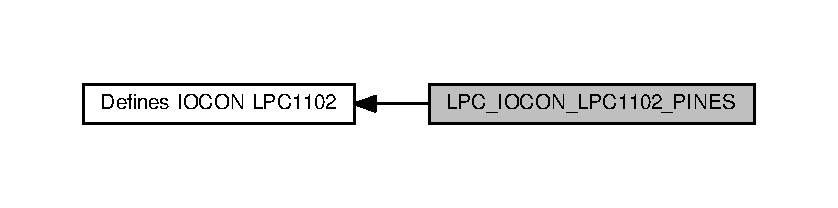
\includegraphics[width=350pt]{group___l_p_c___i_o_c_o_n___l_p_c1102___p_i_n_e_s}
\end{center}
\end{figure}
\subsection*{C1 -\/ R\+E\+S\+E\+T/\+P0.0}
\begin{DoxyCompactItemize}
\item 
\#define \hyperlink{group___l_p_c___i_o_c_o_n___l_p_c1102___p_i_n_e_s_gac743a21ae6fb018103e15efe2ea9487e}{L\+P\+C\+\_\+\+I\+O\+C\+O\+N\+\_\+\+C1\+\_\+\+F\+U\+N\+C\+\_\+\+R\+E\+S\+ET}~(0x00000000\+U\+L) $<$$<$ L\+P\+C\+\_\+\+I\+O\+C\+O\+N\+\_\+\+F\+U\+N\+C\+\_\+\+B\+IT
\item 
\#define \hyperlink{group___l_p_c___i_o_c_o_n___l_p_c1102___p_i_n_e_s_gafade20b5f097f138815526a37ea5b86e}{L\+P\+C\+\_\+\+I\+O\+C\+O\+N\+\_\+\+C1\+\_\+\+F\+U\+N\+C\+\_\+\+P\+I\+O0\+\_\+0}~(0x00000001\+U\+L) $<$$<$ L\+P\+C\+\_\+\+I\+O\+C\+O\+N\+\_\+\+F\+U\+N\+C\+\_\+\+B\+IT
\end{DoxyCompactItemize}
\subsection*{A2 -\/ P0.8/\+M\+I\+S\+O/\+C\+T16\+B0\+\_\+\+M\+A\+T0}
\begin{DoxyCompactItemize}
\item 
\#define \hyperlink{group___l_p_c___i_o_c_o_n___l_p_c1102___p_i_n_e_s_ga73249c352adc2c4eb07089edf856904e}{L\+P\+C\+\_\+\+I\+O\+C\+O\+N\+\_\+\+A2\+\_\+\+F\+U\+N\+C\+\_\+\+P\+I\+O0\+\_\+8}~(0x00000000\+U\+L) $<$$<$ L\+P\+C\+\_\+\+I\+O\+C\+O\+N\+\_\+\+F\+U\+N\+C\+\_\+\+B\+IT
\item 
\#define \hyperlink{group___l_p_c___i_o_c_o_n___l_p_c1102___p_i_n_e_s_gac2cf122fa3f708da105cdeba5c33215c}{L\+P\+C\+\_\+\+I\+O\+C\+O\+N\+\_\+\+A2\+\_\+\+F\+U\+N\+C\+\_\+\+M\+I\+S\+O0}~(0x00000001\+U\+L) $<$$<$ L\+P\+C\+\_\+\+I\+O\+C\+O\+N\+\_\+\+F\+U\+N\+C\+\_\+\+B\+IT
\item 
\#define \hyperlink{group___l_p_c___i_o_c_o_n___l_p_c1102___p_i_n_e_s_gae8b3d16d47cc34abc8668f6e5a9ef62b}{L\+P\+C\+\_\+\+I\+O\+C\+O\+N\+\_\+\+A2\+\_\+\+F\+U\+N\+C\+\_\+\+C\+T16\+B0\+\_\+\+M\+A\+T0}~(0x00000002\+U\+L) $<$$<$ L\+P\+C\+\_\+\+I\+O\+C\+O\+N\+\_\+\+F\+U\+N\+C\+\_\+\+B\+IT
\end{DoxyCompactItemize}
\subsection*{A3 -\/ P0.9/\+M\+O\+S\+I/\+C\+T16\+B0\+\_\+\+M\+A\+T1}
\begin{DoxyCompactItemize}
\item 
\#define \hyperlink{group___l_p_c___i_o_c_o_n___l_p_c1102___p_i_n_e_s_gab2f89db29fd04f6a1d1c3111cd3da9f2}{L\+P\+C\+\_\+\+I\+O\+C\+O\+N\+\_\+\+A3\+\_\+\+F\+U\+N\+C\+\_\+\+P\+I\+O0\+\_\+9}~(0x00000000\+U\+L) $<$$<$ L\+P\+C\+\_\+\+I\+O\+C\+O\+N\+\_\+\+F\+U\+N\+C\+\_\+\+B\+IT
\item 
\#define \hyperlink{group___l_p_c___i_o_c_o_n___l_p_c1102___p_i_n_e_s_ga75592faa0d4e235173f790ee80e79651}{L\+P\+C\+\_\+\+I\+O\+C\+O\+N\+\_\+\+A3\+\_\+\+F\+U\+N\+C\+\_\+\+M\+O\+S\+I0}~(0x00000001\+U\+L) $<$$<$ L\+P\+C\+\_\+\+I\+O\+C\+O\+N\+\_\+\+F\+U\+N\+C\+\_\+\+B\+IT
\item 
\#define \hyperlink{group___l_p_c___i_o_c_o_n___l_p_c1102___p_i_n_e_s_gab8c36d6638e434a9db7d3e43e4a5e768}{L\+P\+C\+\_\+\+I\+O\+C\+O\+N\+\_\+\+A3\+\_\+\+F\+U\+N\+C\+\_\+\+C\+T16\+B0\+\_\+\+M\+A\+T1}~(0x00000002\+U\+L) $<$$<$ L\+P\+C\+\_\+\+I\+O\+C\+O\+N\+\_\+\+F\+U\+N\+C\+\_\+\+B\+IT
\end{DoxyCompactItemize}
\subsection*{A4 -\/ S\+W\+C\+L\+K/\+P0.10/\+S\+C\+K0/\+C\+T16\+B0\+\_\+\+M\+A\+T2}
\begin{DoxyCompactItemize}
\item 
\#define \hyperlink{group___l_p_c___i_o_c_o_n___l_p_c1102___p_i_n_e_s_ga71ead8726fc622434f9b4222c5778f60}{L\+P\+C\+\_\+\+I\+O\+C\+O\+N\+\_\+\+A4\+\_\+\+F\+U\+N\+C\+\_\+\+S\+W\+C\+LK}~(0x00000000\+U\+L) $<$$<$ L\+P\+C\+\_\+\+I\+O\+C\+O\+N\+\_\+\+F\+U\+N\+C\+\_\+\+B\+IT
\item 
\#define \hyperlink{group___l_p_c___i_o_c_o_n___l_p_c1102___p_i_n_e_s_ga87cbf13f8963feae2c0ed0efa8207443}{L\+P\+C\+\_\+\+I\+O\+C\+O\+N\+\_\+\+A4\+\_\+\+F\+U\+N\+C\+\_\+\+P\+I\+O0\+\_\+10}~(0x00000001\+U\+L) $<$$<$ L\+P\+C\+\_\+\+I\+O\+C\+O\+N\+\_\+\+F\+U\+N\+C\+\_\+\+B\+IT
\item 
\#define \hyperlink{group___l_p_c___i_o_c_o_n___l_p_c1102___p_i_n_e_s_ga15f501e83044f160bad331f583ff0de2}{L\+P\+C\+\_\+\+I\+O\+C\+O\+N\+\_\+\+A4\+\_\+\+F\+U\+N\+C\+\_\+\+S\+C\+K0}~(0x00000002\+U\+L) $<$$<$ L\+P\+C\+\_\+\+I\+O\+C\+O\+N\+\_\+\+F\+U\+N\+C\+\_\+\+B\+IT
\item 
\#define \hyperlink{group___l_p_c___i_o_c_o_n___l_p_c1102___p_i_n_e_s_ga1d8317d7eab94b27acec3dd6566e1603}{L\+P\+C\+\_\+\+I\+O\+C\+O\+N\+\_\+\+A4\+\_\+\+F\+U\+N\+C\+\_\+\+C\+T16\+B0\+\_\+\+M\+A\+T2}~(0x00000003\+U\+L) $<$$<$ L\+P\+C\+\_\+\+I\+O\+C\+O\+N\+\_\+\+F\+U\+N\+C\+\_\+\+B\+IT
\end{DoxyCompactItemize}
\subsection*{B4 -\/ R/\+P0.11/\+A\+D0/\+C\+T32\+B0\+\_\+\+M\+A\+T3}
\begin{DoxyCompactItemize}
\item 
\#define \hyperlink{group___l_p_c___i_o_c_o_n___l_p_c1102___p_i_n_e_s_gaaf9bca59195d557afe0706795adde87b}{L\+P\+C\+\_\+\+I\+O\+C\+O\+N\+\_\+\+B4\+\_\+\+F\+U\+N\+C\+\_\+R}~(0x00000000\+U\+L) $<$$<$ L\+P\+C\+\_\+\+I\+O\+C\+O\+N\+\_\+\+F\+U\+N\+C\+\_\+\+B\+IT
\item 
\#define \hyperlink{group___l_p_c___i_o_c_o_n___l_p_c1102___p_i_n_e_s_ga772b2ba88b3dbd3457e63a5e41a52a05}{L\+P\+C\+\_\+\+I\+O\+C\+O\+N\+\_\+\+B4\+\_\+\+F\+U\+N\+C\+\_\+\+P\+I\+O0\+\_\+11}~(0x00000001\+U\+L) $<$$<$ L\+P\+C\+\_\+\+I\+O\+C\+O\+N\+\_\+\+F\+U\+N\+C\+\_\+\+B\+IT
\item 
\#define \hyperlink{group___l_p_c___i_o_c_o_n___l_p_c1102___p_i_n_e_s_gae81155dea1ee849ae1324fbe36b9ebb7}{L\+P\+C\+\_\+\+I\+O\+C\+O\+N\+\_\+\+B4\+\_\+\+F\+U\+N\+C\+\_\+\+A\+D0}~(0x00000002\+U\+L) $<$$<$ L\+P\+C\+\_\+\+I\+O\+C\+O\+N\+\_\+\+F\+U\+N\+C\+\_\+\+B\+IT
\item 
\#define \hyperlink{group___l_p_c___i_o_c_o_n___l_p_c1102___p_i_n_e_s_gaf233dc12f01fa1193a2c8916c7b62960}{L\+P\+C\+\_\+\+I\+O\+C\+O\+N\+\_\+\+B4\+\_\+\+F\+U\+N\+C\+\_\+\+C\+T16\+B0\+\_\+\+M\+A\+T3}~(0x00000003\+U\+L) $<$$<$ L\+P\+C\+\_\+\+I\+O\+C\+O\+N\+\_\+\+F\+U\+N\+C\+\_\+\+B\+IT
\end{DoxyCompactItemize}
\subsection*{B3 -\/ R/\+P1.0/\+A\+D1/\+C\+T32\+B1\+\_\+\+C\+A\+P0}
\begin{DoxyCompactItemize}
\item 
\#define \hyperlink{group___l_p_c___i_o_c_o_n___l_p_c1102___p_i_n_e_s_ga745545f76e10bc8663d8abf205ce3417}{L\+P\+C\+\_\+\+I\+O\+C\+O\+N\+\_\+\+B3\+\_\+\+F\+U\+N\+C\+\_\+R}~(0x00000000\+U\+L) $<$$<$ L\+P\+C\+\_\+\+I\+O\+C\+O\+N\+\_\+\+F\+U\+N\+C\+\_\+\+B\+IT
\item 
\#define \hyperlink{group___l_p_c___i_o_c_o_n___l_p_c1102___p_i_n_e_s_ga05526127ae3fdce2a8b9d838e7c0f6d0}{L\+P\+C\+\_\+\+I\+O\+C\+O\+N\+\_\+\+B3\+\_\+\+F\+U\+N\+C\+\_\+\+P\+I\+O1\+\_\+0}~(0x00000001\+U\+L) $<$$<$ L\+P\+C\+\_\+\+I\+O\+C\+O\+N\+\_\+\+F\+U\+N\+C\+\_\+\+B\+IT
\item 
\#define \hyperlink{group___l_p_c___i_o_c_o_n___l_p_c1102___p_i_n_e_s_gaf638fc4d9aea6f2b8f9b5bf1ab0f6942}{L\+P\+C\+\_\+\+I\+O\+C\+O\+N\+\_\+\+B3\+\_\+\+F\+U\+N\+C\+\_\+\+A\+D1}~(0x00000002\+U\+L) $<$$<$ L\+P\+C\+\_\+\+I\+O\+C\+O\+N\+\_\+\+F\+U\+N\+C\+\_\+\+B\+IT
\item 
\#define \hyperlink{group___l_p_c___i_o_c_o_n___l_p_c1102___p_i_n_e_s_gad92721a2f17acdc507bde9b386b6517a}{L\+P\+C\+\_\+\+I\+O\+C\+O\+N\+\_\+\+B3\+\_\+\+F\+U\+N\+C\+\_\+\+C\+T32\+B1\+\_\+\+C\+A\+P0}~(0x00000003\+U\+L) $<$$<$ L\+P\+C\+\_\+\+I\+O\+C\+O\+N\+\_\+\+F\+U\+N\+C\+\_\+\+B\+IT
\end{DoxyCompactItemize}
\subsection*{C4 -\/ R/\+P1.1/\+A\+D2/\+C\+T32\+B1\+\_\+\+M\+A\+T0}
\begin{DoxyCompactItemize}
\item 
\#define \hyperlink{group___l_p_c___i_o_c_o_n___l_p_c1102___p_i_n_e_s_ga5109d5a6418fa651ad73bc316a2ca64d}{L\+P\+C\+\_\+\+I\+O\+C\+O\+N\+\_\+\+C4\+\_\+\+F\+U\+N\+C\+\_\+R}~(0x00000000\+U\+L) $<$$<$ L\+P\+C\+\_\+\+I\+O\+C\+O\+N\+\_\+\+F\+U\+N\+C\+\_\+\+B\+IT
\item 
\#define \hyperlink{group___l_p_c___i_o_c_o_n___l_p_c1102___p_i_n_e_s_ga68ee6b56ec7c4eea69bb4602a44f2bf3}{L\+P\+C\+\_\+\+I\+O\+C\+O\+N\+\_\+\+C4\+\_\+\+F\+U\+N\+C\+\_\+\+P\+I\+O1\+\_\+1}~(0x00000001\+U\+L) $<$$<$ L\+P\+C\+\_\+\+I\+O\+C\+O\+N\+\_\+\+F\+U\+N\+C\+\_\+\+B\+IT
\item 
\#define \hyperlink{group___l_p_c___i_o_c_o_n___l_p_c1102___p_i_n_e_s_gad03ecd173dbeb860f3ef155bf598debc}{L\+P\+C\+\_\+\+I\+O\+C\+O\+N\+\_\+\+C4\+\_\+\+F\+U\+N\+C\+\_\+\+A\+D2}~(0x00000002\+U\+L) $<$$<$ L\+P\+C\+\_\+\+I\+O\+C\+O\+N\+\_\+\+F\+U\+N\+C\+\_\+\+B\+IT
\item 
\#define \hyperlink{group___l_p_c___i_o_c_o_n___l_p_c1102___p_i_n_e_s_gad9da73ec7045034730c0ac2540a34c16}{L\+P\+C\+\_\+\+I\+O\+C\+O\+N\+\_\+\+C4\+\_\+\+F\+U\+N\+C\+\_\+\+C\+T32\+B1\+\_\+\+M\+A\+T0}~(0x00000003\+U\+L) $<$$<$ L\+P\+C\+\_\+\+I\+O\+C\+O\+N\+\_\+\+F\+U\+N\+C\+\_\+\+B\+IT
\end{DoxyCompactItemize}
\subsection*{C3 -\/ R/\+P1.2/\+A\+D3/\+C\+T32\+B1\+\_\+\+M\+A\+T1}
\begin{DoxyCompactItemize}
\item 
\#define \hyperlink{group___l_p_c___i_o_c_o_n___l_p_c1102___p_i_n_e_s_ga0ce0c613a070b5c4df0d5cc9ceda8295}{L\+P\+C\+\_\+\+I\+O\+C\+O\+N\+\_\+\+C3\+\_\+\+F\+U\+N\+C\+\_\+R}~(0x00000000\+U\+L) $<$$<$ L\+P\+C\+\_\+\+I\+O\+C\+O\+N\+\_\+\+F\+U\+N\+C\+\_\+\+B\+IT
\item 
\#define \hyperlink{group___l_p_c___i_o_c_o_n___l_p_c1102___p_i_n_e_s_ga0a8c9225a9d80bf16239e67d7e321bf3}{L\+P\+C\+\_\+\+I\+O\+C\+O\+N\+\_\+\+C3\+\_\+\+F\+U\+N\+C\+\_\+\+P\+I\+O1\+\_\+2}~(0x00000001\+U\+L) $<$$<$ L\+P\+C\+\_\+\+I\+O\+C\+O\+N\+\_\+\+F\+U\+N\+C\+\_\+\+B\+IT
\item 
\#define \hyperlink{group___l_p_c___i_o_c_o_n___l_p_c1102___p_i_n_e_s_ga3ba9a8b0b1234e4b1d8d8f2ebf5cbec6}{L\+P\+C\+\_\+\+I\+O\+C\+O\+N\+\_\+\+C3\+\_\+\+F\+U\+N\+C\+\_\+\+A\+D3}~(0x00000002\+U\+L) $<$$<$ L\+P\+C\+\_\+\+I\+O\+C\+O\+N\+\_\+\+F\+U\+N\+C\+\_\+\+B\+IT
\item 
\#define \hyperlink{group___l_p_c___i_o_c_o_n___l_p_c1102___p_i_n_e_s_gafb52d80ad556237649f92c38416825d3}{L\+P\+C\+\_\+\+I\+O\+C\+O\+N\+\_\+\+C3\+\_\+\+F\+U\+N\+C\+\_\+\+C\+T32\+B1\+\_\+\+M\+A\+T1}~(0x00000003\+U\+L) $<$$<$ L\+P\+C\+\_\+\+I\+O\+C\+O\+N\+\_\+\+F\+U\+N\+C\+\_\+\+B\+IT
\end{DoxyCompactItemize}
\subsection*{D4 -\/ S\+W\+D\+I\+O/\+P1.3/\+A\+D4/\+C\+T32\+B1\+\_\+\+M\+A\+T2}
\begin{DoxyCompactItemize}
\item 
\#define \hyperlink{group___l_p_c___i_o_c_o_n___l_p_c1102___p_i_n_e_s_ga7d0843dbf1f39f41e01cdcf0ea1396f8}{L\+P\+C\+\_\+\+I\+O\+C\+O\+N\+\_\+\+D4\+\_\+\+F\+U\+N\+C\+\_\+\+S\+W\+D\+IO}~(0x00000000\+U\+L) $<$$<$ L\+P\+C\+\_\+\+I\+O\+C\+O\+N\+\_\+\+F\+U\+N\+C\+\_\+\+B\+IT
\item 
\#define \hyperlink{group___l_p_c___i_o_c_o_n___l_p_c1102___p_i_n_e_s_ga029a20695f231fa2f81d7bd0642a6f85}{L\+P\+C\+\_\+\+I\+O\+C\+O\+N\+\_\+\+D4\+\_\+\+F\+U\+N\+C\+\_\+\+P\+I\+O1\+\_\+3}~(0x00000001\+U\+L) $<$$<$ L\+P\+C\+\_\+\+I\+O\+C\+O\+N\+\_\+\+F\+U\+N\+C\+\_\+\+B\+IT
\item 
\#define \hyperlink{group___l_p_c___i_o_c_o_n___l_p_c1102___p_i_n_e_s_ga73cef70ce7760ccd240ddf0b26a33656}{L\+P\+C\+\_\+\+I\+O\+C\+O\+N\+\_\+\+D4\+\_\+\+F\+U\+N\+C\+\_\+\+A\+D4}~(0x00000002\+U\+L) $<$$<$ L\+P\+C\+\_\+\+I\+O\+C\+O\+N\+\_\+\+F\+U\+N\+C\+\_\+\+B\+IT
\item 
\#define \hyperlink{group___l_p_c___i_o_c_o_n___l_p_c1102___p_i_n_e_s_ga07986c77c1b43eb5994da559abfda911}{L\+P\+C\+\_\+\+I\+O\+C\+O\+N\+\_\+\+D4\+\_\+\+F\+U\+N\+C\+\_\+\+C\+T32\+B1\+\_\+\+M\+A\+T2}~(0x00000003\+U\+L) $<$$<$ L\+P\+C\+\_\+\+I\+O\+C\+O\+N\+\_\+\+F\+U\+N\+C\+\_\+\+B\+IT
\end{DoxyCompactItemize}
\subsection*{C2 -\/ P1.6/\+R\+X\+D/\+C\+T32\+B0\+\_\+\+M\+A\+T0}
\begin{DoxyCompactItemize}
\item 
\#define \hyperlink{group___l_p_c___i_o_c_o_n___l_p_c1102___p_i_n_e_s_ga0f09acebc3f44b34a3b2a42a13888bd4}{L\+P\+C\+\_\+\+I\+O\+C\+O\+N\+\_\+\+C2\+\_\+\+F\+U\+N\+C\+\_\+\+P\+I\+O1\+\_\+3}~(0x00000000\+U\+L) $<$$<$ L\+P\+C\+\_\+\+I\+O\+C\+O\+N\+\_\+\+F\+U\+N\+C\+\_\+\+B\+IT
\item 
\#define \hyperlink{group___l_p_c___i_o_c_o_n___l_p_c1102___p_i_n_e_s_ga2d578e6a171300d7662cbc772e561709}{L\+P\+C\+\_\+\+I\+O\+C\+O\+N\+\_\+\+C2\+\_\+\+F\+U\+N\+C\+\_\+\+R\+XD}~(0x00000001\+U\+L) $<$$<$ L\+P\+C\+\_\+\+I\+O\+C\+O\+N\+\_\+\+F\+U\+N\+C\+\_\+\+B\+IT
\item 
\#define \hyperlink{group___l_p_c___i_o_c_o_n___l_p_c1102___p_i_n_e_s_ga747cbcdca6a691c32f20216f8d25b0c1}{L\+P\+C\+\_\+\+I\+O\+C\+O\+N\+\_\+\+C4\+\_\+\+F\+U\+N\+C\+\_\+\+C\+T32\+B0\+\_\+\+M\+A\+T0}~(0x00000002\+U\+L) $<$$<$ L\+P\+C\+\_\+\+I\+O\+C\+O\+N\+\_\+\+F\+U\+N\+C\+\_\+\+B\+IT
\end{DoxyCompactItemize}
\subsection*{D1 -\/ P1.7/\+T\+X\+D/\+C\+T32\+B0\+\_\+\+M\+A\+T1}
\begin{DoxyCompactItemize}
\item 
\#define \hyperlink{group___l_p_c___i_o_c_o_n___l_p_c1102___p_i_n_e_s_gaffb3310b8c854e58d1f5e3c2449df182}{L\+P\+C\+\_\+\+I\+O\+C\+O\+N\+\_\+\+D1\+\_\+\+F\+U\+N\+C\+\_\+\+P\+I\+O1\+\_\+7}~(0x00000000\+U\+L) $<$$<$ L\+P\+C\+\_\+\+I\+O\+C\+O\+N\+\_\+\+F\+U\+N\+C\+\_\+\+B\+IT
\item 
\#define \hyperlink{group___l_p_c___i_o_c_o_n___l_p_c1102___p_i_n_e_s_ga20f8d9546ce4f038a1546f542241ba86}{L\+P\+C\+\_\+\+I\+O\+C\+O\+N\+\_\+\+D1\+\_\+\+F\+U\+N\+C\+\_\+\+T\+XD}~(0x00000001\+U\+L) $<$$<$ L\+P\+C\+\_\+\+I\+O\+C\+O\+N\+\_\+\+F\+U\+N\+C\+\_\+\+B\+IT
\item 
\#define \hyperlink{group___l_p_c___i_o_c_o_n___l_p_c1102___p_i_n_e_s_ga3f3e6bd87d14b9164bf95b99abbd2461}{L\+P\+C\+\_\+\+I\+O\+C\+O\+N\+\_\+\+D1\+\_\+\+F\+U\+N\+C\+\_\+\+C\+T32\+B0\+\_\+\+M\+A\+T1}~(0x00000002\+U\+L) $<$$<$ L\+P\+C\+\_\+\+I\+O\+C\+O\+N\+\_\+\+F\+U\+N\+C\+\_\+\+B\+IT
\end{DoxyCompactItemize}


\subsection{Detailed Description}
Funciones de cada pin asociados a los registros I\+O\+C\+ON. 



\subsection{Macro Definition Documentation}
\index{L\+P\+C\+\_\+\+I\+O\+C\+O\+N\+\_\+\+L\+P\+C1102\+\_\+\+P\+I\+N\+ES@{L\+P\+C\+\_\+\+I\+O\+C\+O\+N\+\_\+\+L\+P\+C1102\+\_\+\+P\+I\+N\+ES}!L\+P\+C\+\_\+\+I\+O\+C\+O\+N\+\_\+\+A2\+\_\+\+F\+U\+N\+C\+\_\+\+C\+T16\+B0\+\_\+\+M\+A\+T0@{L\+P\+C\+\_\+\+I\+O\+C\+O\+N\+\_\+\+A2\+\_\+\+F\+U\+N\+C\+\_\+\+C\+T16\+B0\+\_\+\+M\+A\+T0}}
\index{L\+P\+C\+\_\+\+I\+O\+C\+O\+N\+\_\+\+A2\+\_\+\+F\+U\+N\+C\+\_\+\+C\+T16\+B0\+\_\+\+M\+A\+T0@{L\+P\+C\+\_\+\+I\+O\+C\+O\+N\+\_\+\+A2\+\_\+\+F\+U\+N\+C\+\_\+\+C\+T16\+B0\+\_\+\+M\+A\+T0}!L\+P\+C\+\_\+\+I\+O\+C\+O\+N\+\_\+\+L\+P\+C1102\+\_\+\+P\+I\+N\+ES@{L\+P\+C\+\_\+\+I\+O\+C\+O\+N\+\_\+\+L\+P\+C1102\+\_\+\+P\+I\+N\+ES}}
\subsubsection[{\texorpdfstring{L\+P\+C\+\_\+\+I\+O\+C\+O\+N\+\_\+\+A2\+\_\+\+F\+U\+N\+C\+\_\+\+C\+T16\+B0\+\_\+\+M\+A\+T0}{LPC_IOCON_A2_FUNC_CT16B0_MAT0}}]{\setlength{\rightskip}{0pt plus 5cm}\#define L\+P\+C\+\_\+\+I\+O\+C\+O\+N\+\_\+\+A2\+\_\+\+F\+U\+N\+C\+\_\+\+C\+T16\+B0\+\_\+\+M\+A\+T0~(0x00000002\+U\+L) $<$$<$ L\+P\+C\+\_\+\+I\+O\+C\+O\+N\+\_\+\+F\+U\+N\+C\+\_\+\+B\+IT}\hypertarget{group___l_p_c___i_o_c_o_n___l_p_c1102___p_i_n_e_s_gae8b3d16d47cc34abc8668f6e5a9ef62b}{}\label{group___l_p_c___i_o_c_o_n___l_p_c1102___p_i_n_e_s_gae8b3d16d47cc34abc8668f6e5a9ef62b}


Definition at line 88 of file L\+P\+C1102\+\_\+\+I\+O\+C\+O\+N.\+h.

\index{L\+P\+C\+\_\+\+I\+O\+C\+O\+N\+\_\+\+L\+P\+C1102\+\_\+\+P\+I\+N\+ES@{L\+P\+C\+\_\+\+I\+O\+C\+O\+N\+\_\+\+L\+P\+C1102\+\_\+\+P\+I\+N\+ES}!L\+P\+C\+\_\+\+I\+O\+C\+O\+N\+\_\+\+A2\+\_\+\+F\+U\+N\+C\+\_\+\+M\+I\+S\+O0@{L\+P\+C\+\_\+\+I\+O\+C\+O\+N\+\_\+\+A2\+\_\+\+F\+U\+N\+C\+\_\+\+M\+I\+S\+O0}}
\index{L\+P\+C\+\_\+\+I\+O\+C\+O\+N\+\_\+\+A2\+\_\+\+F\+U\+N\+C\+\_\+\+M\+I\+S\+O0@{L\+P\+C\+\_\+\+I\+O\+C\+O\+N\+\_\+\+A2\+\_\+\+F\+U\+N\+C\+\_\+\+M\+I\+S\+O0}!L\+P\+C\+\_\+\+I\+O\+C\+O\+N\+\_\+\+L\+P\+C1102\+\_\+\+P\+I\+N\+ES@{L\+P\+C\+\_\+\+I\+O\+C\+O\+N\+\_\+\+L\+P\+C1102\+\_\+\+P\+I\+N\+ES}}
\subsubsection[{\texorpdfstring{L\+P\+C\+\_\+\+I\+O\+C\+O\+N\+\_\+\+A2\+\_\+\+F\+U\+N\+C\+\_\+\+M\+I\+S\+O0}{LPC_IOCON_A2_FUNC_MISO0}}]{\setlength{\rightskip}{0pt plus 5cm}\#define L\+P\+C\+\_\+\+I\+O\+C\+O\+N\+\_\+\+A2\+\_\+\+F\+U\+N\+C\+\_\+\+M\+I\+S\+O0~(0x00000001\+U\+L) $<$$<$ L\+P\+C\+\_\+\+I\+O\+C\+O\+N\+\_\+\+F\+U\+N\+C\+\_\+\+B\+IT}\hypertarget{group___l_p_c___i_o_c_o_n___l_p_c1102___p_i_n_e_s_gac2cf122fa3f708da105cdeba5c33215c}{}\label{group___l_p_c___i_o_c_o_n___l_p_c1102___p_i_n_e_s_gac2cf122fa3f708da105cdeba5c33215c}


Definition at line 87 of file L\+P\+C1102\+\_\+\+I\+O\+C\+O\+N.\+h.

\index{L\+P\+C\+\_\+\+I\+O\+C\+O\+N\+\_\+\+L\+P\+C1102\+\_\+\+P\+I\+N\+ES@{L\+P\+C\+\_\+\+I\+O\+C\+O\+N\+\_\+\+L\+P\+C1102\+\_\+\+P\+I\+N\+ES}!L\+P\+C\+\_\+\+I\+O\+C\+O\+N\+\_\+\+A2\+\_\+\+F\+U\+N\+C\+\_\+\+P\+I\+O0\+\_\+8@{L\+P\+C\+\_\+\+I\+O\+C\+O\+N\+\_\+\+A2\+\_\+\+F\+U\+N\+C\+\_\+\+P\+I\+O0\+\_\+8}}
\index{L\+P\+C\+\_\+\+I\+O\+C\+O\+N\+\_\+\+A2\+\_\+\+F\+U\+N\+C\+\_\+\+P\+I\+O0\+\_\+8@{L\+P\+C\+\_\+\+I\+O\+C\+O\+N\+\_\+\+A2\+\_\+\+F\+U\+N\+C\+\_\+\+P\+I\+O0\+\_\+8}!L\+P\+C\+\_\+\+I\+O\+C\+O\+N\+\_\+\+L\+P\+C1102\+\_\+\+P\+I\+N\+ES@{L\+P\+C\+\_\+\+I\+O\+C\+O\+N\+\_\+\+L\+P\+C1102\+\_\+\+P\+I\+N\+ES}}
\subsubsection[{\texorpdfstring{L\+P\+C\+\_\+\+I\+O\+C\+O\+N\+\_\+\+A2\+\_\+\+F\+U\+N\+C\+\_\+\+P\+I\+O0\+\_\+8}{LPC_IOCON_A2_FUNC_PIO0_8}}]{\setlength{\rightskip}{0pt plus 5cm}\#define L\+P\+C\+\_\+\+I\+O\+C\+O\+N\+\_\+\+A2\+\_\+\+F\+U\+N\+C\+\_\+\+P\+I\+O0\+\_\+8~(0x00000000\+U\+L) $<$$<$ L\+P\+C\+\_\+\+I\+O\+C\+O\+N\+\_\+\+F\+U\+N\+C\+\_\+\+B\+IT}\hypertarget{group___l_p_c___i_o_c_o_n___l_p_c1102___p_i_n_e_s_ga73249c352adc2c4eb07089edf856904e}{}\label{group___l_p_c___i_o_c_o_n___l_p_c1102___p_i_n_e_s_ga73249c352adc2c4eb07089edf856904e}


Definition at line 86 of file L\+P\+C1102\+\_\+\+I\+O\+C\+O\+N.\+h.

\index{L\+P\+C\+\_\+\+I\+O\+C\+O\+N\+\_\+\+L\+P\+C1102\+\_\+\+P\+I\+N\+ES@{L\+P\+C\+\_\+\+I\+O\+C\+O\+N\+\_\+\+L\+P\+C1102\+\_\+\+P\+I\+N\+ES}!L\+P\+C\+\_\+\+I\+O\+C\+O\+N\+\_\+\+A3\+\_\+\+F\+U\+N\+C\+\_\+\+C\+T16\+B0\+\_\+\+M\+A\+T1@{L\+P\+C\+\_\+\+I\+O\+C\+O\+N\+\_\+\+A3\+\_\+\+F\+U\+N\+C\+\_\+\+C\+T16\+B0\+\_\+\+M\+A\+T1}}
\index{L\+P\+C\+\_\+\+I\+O\+C\+O\+N\+\_\+\+A3\+\_\+\+F\+U\+N\+C\+\_\+\+C\+T16\+B0\+\_\+\+M\+A\+T1@{L\+P\+C\+\_\+\+I\+O\+C\+O\+N\+\_\+\+A3\+\_\+\+F\+U\+N\+C\+\_\+\+C\+T16\+B0\+\_\+\+M\+A\+T1}!L\+P\+C\+\_\+\+I\+O\+C\+O\+N\+\_\+\+L\+P\+C1102\+\_\+\+P\+I\+N\+ES@{L\+P\+C\+\_\+\+I\+O\+C\+O\+N\+\_\+\+L\+P\+C1102\+\_\+\+P\+I\+N\+ES}}
\subsubsection[{\texorpdfstring{L\+P\+C\+\_\+\+I\+O\+C\+O\+N\+\_\+\+A3\+\_\+\+F\+U\+N\+C\+\_\+\+C\+T16\+B0\+\_\+\+M\+A\+T1}{LPC_IOCON_A3_FUNC_CT16B0_MAT1}}]{\setlength{\rightskip}{0pt plus 5cm}\#define L\+P\+C\+\_\+\+I\+O\+C\+O\+N\+\_\+\+A3\+\_\+\+F\+U\+N\+C\+\_\+\+C\+T16\+B0\+\_\+\+M\+A\+T1~(0x00000002\+U\+L) $<$$<$ L\+P\+C\+\_\+\+I\+O\+C\+O\+N\+\_\+\+F\+U\+N\+C\+\_\+\+B\+IT}\hypertarget{group___l_p_c___i_o_c_o_n___l_p_c1102___p_i_n_e_s_gab8c36d6638e434a9db7d3e43e4a5e768}{}\label{group___l_p_c___i_o_c_o_n___l_p_c1102___p_i_n_e_s_gab8c36d6638e434a9db7d3e43e4a5e768}


Definition at line 98 of file L\+P\+C1102\+\_\+\+I\+O\+C\+O\+N.\+h.

\index{L\+P\+C\+\_\+\+I\+O\+C\+O\+N\+\_\+\+L\+P\+C1102\+\_\+\+P\+I\+N\+ES@{L\+P\+C\+\_\+\+I\+O\+C\+O\+N\+\_\+\+L\+P\+C1102\+\_\+\+P\+I\+N\+ES}!L\+P\+C\+\_\+\+I\+O\+C\+O\+N\+\_\+\+A3\+\_\+\+F\+U\+N\+C\+\_\+\+M\+O\+S\+I0@{L\+P\+C\+\_\+\+I\+O\+C\+O\+N\+\_\+\+A3\+\_\+\+F\+U\+N\+C\+\_\+\+M\+O\+S\+I0}}
\index{L\+P\+C\+\_\+\+I\+O\+C\+O\+N\+\_\+\+A3\+\_\+\+F\+U\+N\+C\+\_\+\+M\+O\+S\+I0@{L\+P\+C\+\_\+\+I\+O\+C\+O\+N\+\_\+\+A3\+\_\+\+F\+U\+N\+C\+\_\+\+M\+O\+S\+I0}!L\+P\+C\+\_\+\+I\+O\+C\+O\+N\+\_\+\+L\+P\+C1102\+\_\+\+P\+I\+N\+ES@{L\+P\+C\+\_\+\+I\+O\+C\+O\+N\+\_\+\+L\+P\+C1102\+\_\+\+P\+I\+N\+ES}}
\subsubsection[{\texorpdfstring{L\+P\+C\+\_\+\+I\+O\+C\+O\+N\+\_\+\+A3\+\_\+\+F\+U\+N\+C\+\_\+\+M\+O\+S\+I0}{LPC_IOCON_A3_FUNC_MOSI0}}]{\setlength{\rightskip}{0pt plus 5cm}\#define L\+P\+C\+\_\+\+I\+O\+C\+O\+N\+\_\+\+A3\+\_\+\+F\+U\+N\+C\+\_\+\+M\+O\+S\+I0~(0x00000001\+U\+L) $<$$<$ L\+P\+C\+\_\+\+I\+O\+C\+O\+N\+\_\+\+F\+U\+N\+C\+\_\+\+B\+IT}\hypertarget{group___l_p_c___i_o_c_o_n___l_p_c1102___p_i_n_e_s_ga75592faa0d4e235173f790ee80e79651}{}\label{group___l_p_c___i_o_c_o_n___l_p_c1102___p_i_n_e_s_ga75592faa0d4e235173f790ee80e79651}


Definition at line 97 of file L\+P\+C1102\+\_\+\+I\+O\+C\+O\+N.\+h.

\index{L\+P\+C\+\_\+\+I\+O\+C\+O\+N\+\_\+\+L\+P\+C1102\+\_\+\+P\+I\+N\+ES@{L\+P\+C\+\_\+\+I\+O\+C\+O\+N\+\_\+\+L\+P\+C1102\+\_\+\+P\+I\+N\+ES}!L\+P\+C\+\_\+\+I\+O\+C\+O\+N\+\_\+\+A3\+\_\+\+F\+U\+N\+C\+\_\+\+P\+I\+O0\+\_\+9@{L\+P\+C\+\_\+\+I\+O\+C\+O\+N\+\_\+\+A3\+\_\+\+F\+U\+N\+C\+\_\+\+P\+I\+O0\+\_\+9}}
\index{L\+P\+C\+\_\+\+I\+O\+C\+O\+N\+\_\+\+A3\+\_\+\+F\+U\+N\+C\+\_\+\+P\+I\+O0\+\_\+9@{L\+P\+C\+\_\+\+I\+O\+C\+O\+N\+\_\+\+A3\+\_\+\+F\+U\+N\+C\+\_\+\+P\+I\+O0\+\_\+9}!L\+P\+C\+\_\+\+I\+O\+C\+O\+N\+\_\+\+L\+P\+C1102\+\_\+\+P\+I\+N\+ES@{L\+P\+C\+\_\+\+I\+O\+C\+O\+N\+\_\+\+L\+P\+C1102\+\_\+\+P\+I\+N\+ES}}
\subsubsection[{\texorpdfstring{L\+P\+C\+\_\+\+I\+O\+C\+O\+N\+\_\+\+A3\+\_\+\+F\+U\+N\+C\+\_\+\+P\+I\+O0\+\_\+9}{LPC_IOCON_A3_FUNC_PIO0_9}}]{\setlength{\rightskip}{0pt plus 5cm}\#define L\+P\+C\+\_\+\+I\+O\+C\+O\+N\+\_\+\+A3\+\_\+\+F\+U\+N\+C\+\_\+\+P\+I\+O0\+\_\+9~(0x00000000\+U\+L) $<$$<$ L\+P\+C\+\_\+\+I\+O\+C\+O\+N\+\_\+\+F\+U\+N\+C\+\_\+\+B\+IT}\hypertarget{group___l_p_c___i_o_c_o_n___l_p_c1102___p_i_n_e_s_gab2f89db29fd04f6a1d1c3111cd3da9f2}{}\label{group___l_p_c___i_o_c_o_n___l_p_c1102___p_i_n_e_s_gab2f89db29fd04f6a1d1c3111cd3da9f2}


Definition at line 96 of file L\+P\+C1102\+\_\+\+I\+O\+C\+O\+N.\+h.

\index{L\+P\+C\+\_\+\+I\+O\+C\+O\+N\+\_\+\+L\+P\+C1102\+\_\+\+P\+I\+N\+ES@{L\+P\+C\+\_\+\+I\+O\+C\+O\+N\+\_\+\+L\+P\+C1102\+\_\+\+P\+I\+N\+ES}!L\+P\+C\+\_\+\+I\+O\+C\+O\+N\+\_\+\+A4\+\_\+\+F\+U\+N\+C\+\_\+\+C\+T16\+B0\+\_\+\+M\+A\+T2@{L\+P\+C\+\_\+\+I\+O\+C\+O\+N\+\_\+\+A4\+\_\+\+F\+U\+N\+C\+\_\+\+C\+T16\+B0\+\_\+\+M\+A\+T2}}
\index{L\+P\+C\+\_\+\+I\+O\+C\+O\+N\+\_\+\+A4\+\_\+\+F\+U\+N\+C\+\_\+\+C\+T16\+B0\+\_\+\+M\+A\+T2@{L\+P\+C\+\_\+\+I\+O\+C\+O\+N\+\_\+\+A4\+\_\+\+F\+U\+N\+C\+\_\+\+C\+T16\+B0\+\_\+\+M\+A\+T2}!L\+P\+C\+\_\+\+I\+O\+C\+O\+N\+\_\+\+L\+P\+C1102\+\_\+\+P\+I\+N\+ES@{L\+P\+C\+\_\+\+I\+O\+C\+O\+N\+\_\+\+L\+P\+C1102\+\_\+\+P\+I\+N\+ES}}
\subsubsection[{\texorpdfstring{L\+P\+C\+\_\+\+I\+O\+C\+O\+N\+\_\+\+A4\+\_\+\+F\+U\+N\+C\+\_\+\+C\+T16\+B0\+\_\+\+M\+A\+T2}{LPC_IOCON_A4_FUNC_CT16B0_MAT2}}]{\setlength{\rightskip}{0pt plus 5cm}\#define L\+P\+C\+\_\+\+I\+O\+C\+O\+N\+\_\+\+A4\+\_\+\+F\+U\+N\+C\+\_\+\+C\+T16\+B0\+\_\+\+M\+A\+T2~(0x00000003\+U\+L) $<$$<$ L\+P\+C\+\_\+\+I\+O\+C\+O\+N\+\_\+\+F\+U\+N\+C\+\_\+\+B\+IT}\hypertarget{group___l_p_c___i_o_c_o_n___l_p_c1102___p_i_n_e_s_ga1d8317d7eab94b27acec3dd6566e1603}{}\label{group___l_p_c___i_o_c_o_n___l_p_c1102___p_i_n_e_s_ga1d8317d7eab94b27acec3dd6566e1603}


Definition at line 109 of file L\+P\+C1102\+\_\+\+I\+O\+C\+O\+N.\+h.

\index{L\+P\+C\+\_\+\+I\+O\+C\+O\+N\+\_\+\+L\+P\+C1102\+\_\+\+P\+I\+N\+ES@{L\+P\+C\+\_\+\+I\+O\+C\+O\+N\+\_\+\+L\+P\+C1102\+\_\+\+P\+I\+N\+ES}!L\+P\+C\+\_\+\+I\+O\+C\+O\+N\+\_\+\+A4\+\_\+\+F\+U\+N\+C\+\_\+\+P\+I\+O0\+\_\+10@{L\+P\+C\+\_\+\+I\+O\+C\+O\+N\+\_\+\+A4\+\_\+\+F\+U\+N\+C\+\_\+\+P\+I\+O0\+\_\+10}}
\index{L\+P\+C\+\_\+\+I\+O\+C\+O\+N\+\_\+\+A4\+\_\+\+F\+U\+N\+C\+\_\+\+P\+I\+O0\+\_\+10@{L\+P\+C\+\_\+\+I\+O\+C\+O\+N\+\_\+\+A4\+\_\+\+F\+U\+N\+C\+\_\+\+P\+I\+O0\+\_\+10}!L\+P\+C\+\_\+\+I\+O\+C\+O\+N\+\_\+\+L\+P\+C1102\+\_\+\+P\+I\+N\+ES@{L\+P\+C\+\_\+\+I\+O\+C\+O\+N\+\_\+\+L\+P\+C1102\+\_\+\+P\+I\+N\+ES}}
\subsubsection[{\texorpdfstring{L\+P\+C\+\_\+\+I\+O\+C\+O\+N\+\_\+\+A4\+\_\+\+F\+U\+N\+C\+\_\+\+P\+I\+O0\+\_\+10}{LPC_IOCON_A4_FUNC_PIO0_10}}]{\setlength{\rightskip}{0pt plus 5cm}\#define L\+P\+C\+\_\+\+I\+O\+C\+O\+N\+\_\+\+A4\+\_\+\+F\+U\+N\+C\+\_\+\+P\+I\+O0\+\_\+10~(0x00000001\+U\+L) $<$$<$ L\+P\+C\+\_\+\+I\+O\+C\+O\+N\+\_\+\+F\+U\+N\+C\+\_\+\+B\+IT}\hypertarget{group___l_p_c___i_o_c_o_n___l_p_c1102___p_i_n_e_s_ga87cbf13f8963feae2c0ed0efa8207443}{}\label{group___l_p_c___i_o_c_o_n___l_p_c1102___p_i_n_e_s_ga87cbf13f8963feae2c0ed0efa8207443}


Definition at line 107 of file L\+P\+C1102\+\_\+\+I\+O\+C\+O\+N.\+h.

\index{L\+P\+C\+\_\+\+I\+O\+C\+O\+N\+\_\+\+L\+P\+C1102\+\_\+\+P\+I\+N\+ES@{L\+P\+C\+\_\+\+I\+O\+C\+O\+N\+\_\+\+L\+P\+C1102\+\_\+\+P\+I\+N\+ES}!L\+P\+C\+\_\+\+I\+O\+C\+O\+N\+\_\+\+A4\+\_\+\+F\+U\+N\+C\+\_\+\+S\+C\+K0@{L\+P\+C\+\_\+\+I\+O\+C\+O\+N\+\_\+\+A4\+\_\+\+F\+U\+N\+C\+\_\+\+S\+C\+K0}}
\index{L\+P\+C\+\_\+\+I\+O\+C\+O\+N\+\_\+\+A4\+\_\+\+F\+U\+N\+C\+\_\+\+S\+C\+K0@{L\+P\+C\+\_\+\+I\+O\+C\+O\+N\+\_\+\+A4\+\_\+\+F\+U\+N\+C\+\_\+\+S\+C\+K0}!L\+P\+C\+\_\+\+I\+O\+C\+O\+N\+\_\+\+L\+P\+C1102\+\_\+\+P\+I\+N\+ES@{L\+P\+C\+\_\+\+I\+O\+C\+O\+N\+\_\+\+L\+P\+C1102\+\_\+\+P\+I\+N\+ES}}
\subsubsection[{\texorpdfstring{L\+P\+C\+\_\+\+I\+O\+C\+O\+N\+\_\+\+A4\+\_\+\+F\+U\+N\+C\+\_\+\+S\+C\+K0}{LPC_IOCON_A4_FUNC_SCK0}}]{\setlength{\rightskip}{0pt plus 5cm}\#define L\+P\+C\+\_\+\+I\+O\+C\+O\+N\+\_\+\+A4\+\_\+\+F\+U\+N\+C\+\_\+\+S\+C\+K0~(0x00000002\+U\+L) $<$$<$ L\+P\+C\+\_\+\+I\+O\+C\+O\+N\+\_\+\+F\+U\+N\+C\+\_\+\+B\+IT}\hypertarget{group___l_p_c___i_o_c_o_n___l_p_c1102___p_i_n_e_s_ga15f501e83044f160bad331f583ff0de2}{}\label{group___l_p_c___i_o_c_o_n___l_p_c1102___p_i_n_e_s_ga15f501e83044f160bad331f583ff0de2}


Definition at line 108 of file L\+P\+C1102\+\_\+\+I\+O\+C\+O\+N.\+h.

\index{L\+P\+C\+\_\+\+I\+O\+C\+O\+N\+\_\+\+L\+P\+C1102\+\_\+\+P\+I\+N\+ES@{L\+P\+C\+\_\+\+I\+O\+C\+O\+N\+\_\+\+L\+P\+C1102\+\_\+\+P\+I\+N\+ES}!L\+P\+C\+\_\+\+I\+O\+C\+O\+N\+\_\+\+A4\+\_\+\+F\+U\+N\+C\+\_\+\+S\+W\+C\+LK@{L\+P\+C\+\_\+\+I\+O\+C\+O\+N\+\_\+\+A4\+\_\+\+F\+U\+N\+C\+\_\+\+S\+W\+C\+LK}}
\index{L\+P\+C\+\_\+\+I\+O\+C\+O\+N\+\_\+\+A4\+\_\+\+F\+U\+N\+C\+\_\+\+S\+W\+C\+LK@{L\+P\+C\+\_\+\+I\+O\+C\+O\+N\+\_\+\+A4\+\_\+\+F\+U\+N\+C\+\_\+\+S\+W\+C\+LK}!L\+P\+C\+\_\+\+I\+O\+C\+O\+N\+\_\+\+L\+P\+C1102\+\_\+\+P\+I\+N\+ES@{L\+P\+C\+\_\+\+I\+O\+C\+O\+N\+\_\+\+L\+P\+C1102\+\_\+\+P\+I\+N\+ES}}
\subsubsection[{\texorpdfstring{L\+P\+C\+\_\+\+I\+O\+C\+O\+N\+\_\+\+A4\+\_\+\+F\+U\+N\+C\+\_\+\+S\+W\+C\+LK}{LPC_IOCON_A4_FUNC_SWCLK}}]{\setlength{\rightskip}{0pt plus 5cm}\#define L\+P\+C\+\_\+\+I\+O\+C\+O\+N\+\_\+\+A4\+\_\+\+F\+U\+N\+C\+\_\+\+S\+W\+C\+LK~(0x00000000\+U\+L) $<$$<$ L\+P\+C\+\_\+\+I\+O\+C\+O\+N\+\_\+\+F\+U\+N\+C\+\_\+\+B\+IT}\hypertarget{group___l_p_c___i_o_c_o_n___l_p_c1102___p_i_n_e_s_ga71ead8726fc622434f9b4222c5778f60}{}\label{group___l_p_c___i_o_c_o_n___l_p_c1102___p_i_n_e_s_ga71ead8726fc622434f9b4222c5778f60}


Definition at line 106 of file L\+P\+C1102\+\_\+\+I\+O\+C\+O\+N.\+h.

\index{L\+P\+C\+\_\+\+I\+O\+C\+O\+N\+\_\+\+L\+P\+C1102\+\_\+\+P\+I\+N\+ES@{L\+P\+C\+\_\+\+I\+O\+C\+O\+N\+\_\+\+L\+P\+C1102\+\_\+\+P\+I\+N\+ES}!L\+P\+C\+\_\+\+I\+O\+C\+O\+N\+\_\+\+B3\+\_\+\+F\+U\+N\+C\+\_\+\+A\+D1@{L\+P\+C\+\_\+\+I\+O\+C\+O\+N\+\_\+\+B3\+\_\+\+F\+U\+N\+C\+\_\+\+A\+D1}}
\index{L\+P\+C\+\_\+\+I\+O\+C\+O\+N\+\_\+\+B3\+\_\+\+F\+U\+N\+C\+\_\+\+A\+D1@{L\+P\+C\+\_\+\+I\+O\+C\+O\+N\+\_\+\+B3\+\_\+\+F\+U\+N\+C\+\_\+\+A\+D1}!L\+P\+C\+\_\+\+I\+O\+C\+O\+N\+\_\+\+L\+P\+C1102\+\_\+\+P\+I\+N\+ES@{L\+P\+C\+\_\+\+I\+O\+C\+O\+N\+\_\+\+L\+P\+C1102\+\_\+\+P\+I\+N\+ES}}
\subsubsection[{\texorpdfstring{L\+P\+C\+\_\+\+I\+O\+C\+O\+N\+\_\+\+B3\+\_\+\+F\+U\+N\+C\+\_\+\+A\+D1}{LPC_IOCON_B3_FUNC_AD1}}]{\setlength{\rightskip}{0pt plus 5cm}\#define L\+P\+C\+\_\+\+I\+O\+C\+O\+N\+\_\+\+B3\+\_\+\+F\+U\+N\+C\+\_\+\+A\+D1~(0x00000002\+U\+L) $<$$<$ L\+P\+C\+\_\+\+I\+O\+C\+O\+N\+\_\+\+F\+U\+N\+C\+\_\+\+B\+IT}\hypertarget{group___l_p_c___i_o_c_o_n___l_p_c1102___p_i_n_e_s_gaf638fc4d9aea6f2b8f9b5bf1ab0f6942}{}\label{group___l_p_c___i_o_c_o_n___l_p_c1102___p_i_n_e_s_gaf638fc4d9aea6f2b8f9b5bf1ab0f6942}


Definition at line 131 of file L\+P\+C1102\+\_\+\+I\+O\+C\+O\+N.\+h.

\index{L\+P\+C\+\_\+\+I\+O\+C\+O\+N\+\_\+\+L\+P\+C1102\+\_\+\+P\+I\+N\+ES@{L\+P\+C\+\_\+\+I\+O\+C\+O\+N\+\_\+\+L\+P\+C1102\+\_\+\+P\+I\+N\+ES}!L\+P\+C\+\_\+\+I\+O\+C\+O\+N\+\_\+\+B3\+\_\+\+F\+U\+N\+C\+\_\+\+C\+T32\+B1\+\_\+\+C\+A\+P0@{L\+P\+C\+\_\+\+I\+O\+C\+O\+N\+\_\+\+B3\+\_\+\+F\+U\+N\+C\+\_\+\+C\+T32\+B1\+\_\+\+C\+A\+P0}}
\index{L\+P\+C\+\_\+\+I\+O\+C\+O\+N\+\_\+\+B3\+\_\+\+F\+U\+N\+C\+\_\+\+C\+T32\+B1\+\_\+\+C\+A\+P0@{L\+P\+C\+\_\+\+I\+O\+C\+O\+N\+\_\+\+B3\+\_\+\+F\+U\+N\+C\+\_\+\+C\+T32\+B1\+\_\+\+C\+A\+P0}!L\+P\+C\+\_\+\+I\+O\+C\+O\+N\+\_\+\+L\+P\+C1102\+\_\+\+P\+I\+N\+ES@{L\+P\+C\+\_\+\+I\+O\+C\+O\+N\+\_\+\+L\+P\+C1102\+\_\+\+P\+I\+N\+ES}}
\subsubsection[{\texorpdfstring{L\+P\+C\+\_\+\+I\+O\+C\+O\+N\+\_\+\+B3\+\_\+\+F\+U\+N\+C\+\_\+\+C\+T32\+B1\+\_\+\+C\+A\+P0}{LPC_IOCON_B3_FUNC_CT32B1_CAP0}}]{\setlength{\rightskip}{0pt plus 5cm}\#define L\+P\+C\+\_\+\+I\+O\+C\+O\+N\+\_\+\+B3\+\_\+\+F\+U\+N\+C\+\_\+\+C\+T32\+B1\+\_\+\+C\+A\+P0~(0x00000003\+U\+L) $<$$<$ L\+P\+C\+\_\+\+I\+O\+C\+O\+N\+\_\+\+F\+U\+N\+C\+\_\+\+B\+IT}\hypertarget{group___l_p_c___i_o_c_o_n___l_p_c1102___p_i_n_e_s_gad92721a2f17acdc507bde9b386b6517a}{}\label{group___l_p_c___i_o_c_o_n___l_p_c1102___p_i_n_e_s_gad92721a2f17acdc507bde9b386b6517a}


Definition at line 132 of file L\+P\+C1102\+\_\+\+I\+O\+C\+O\+N.\+h.

\index{L\+P\+C\+\_\+\+I\+O\+C\+O\+N\+\_\+\+L\+P\+C1102\+\_\+\+P\+I\+N\+ES@{L\+P\+C\+\_\+\+I\+O\+C\+O\+N\+\_\+\+L\+P\+C1102\+\_\+\+P\+I\+N\+ES}!L\+P\+C\+\_\+\+I\+O\+C\+O\+N\+\_\+\+B3\+\_\+\+F\+U\+N\+C\+\_\+\+P\+I\+O1\+\_\+0@{L\+P\+C\+\_\+\+I\+O\+C\+O\+N\+\_\+\+B3\+\_\+\+F\+U\+N\+C\+\_\+\+P\+I\+O1\+\_\+0}}
\index{L\+P\+C\+\_\+\+I\+O\+C\+O\+N\+\_\+\+B3\+\_\+\+F\+U\+N\+C\+\_\+\+P\+I\+O1\+\_\+0@{L\+P\+C\+\_\+\+I\+O\+C\+O\+N\+\_\+\+B3\+\_\+\+F\+U\+N\+C\+\_\+\+P\+I\+O1\+\_\+0}!L\+P\+C\+\_\+\+I\+O\+C\+O\+N\+\_\+\+L\+P\+C1102\+\_\+\+P\+I\+N\+ES@{L\+P\+C\+\_\+\+I\+O\+C\+O\+N\+\_\+\+L\+P\+C1102\+\_\+\+P\+I\+N\+ES}}
\subsubsection[{\texorpdfstring{L\+P\+C\+\_\+\+I\+O\+C\+O\+N\+\_\+\+B3\+\_\+\+F\+U\+N\+C\+\_\+\+P\+I\+O1\+\_\+0}{LPC_IOCON_B3_FUNC_PIO1_0}}]{\setlength{\rightskip}{0pt plus 5cm}\#define L\+P\+C\+\_\+\+I\+O\+C\+O\+N\+\_\+\+B3\+\_\+\+F\+U\+N\+C\+\_\+\+P\+I\+O1\+\_\+0~(0x00000001\+U\+L) $<$$<$ L\+P\+C\+\_\+\+I\+O\+C\+O\+N\+\_\+\+F\+U\+N\+C\+\_\+\+B\+IT}\hypertarget{group___l_p_c___i_o_c_o_n___l_p_c1102___p_i_n_e_s_ga05526127ae3fdce2a8b9d838e7c0f6d0}{}\label{group___l_p_c___i_o_c_o_n___l_p_c1102___p_i_n_e_s_ga05526127ae3fdce2a8b9d838e7c0f6d0}


Definition at line 130 of file L\+P\+C1102\+\_\+\+I\+O\+C\+O\+N.\+h.

\index{L\+P\+C\+\_\+\+I\+O\+C\+O\+N\+\_\+\+L\+P\+C1102\+\_\+\+P\+I\+N\+ES@{L\+P\+C\+\_\+\+I\+O\+C\+O\+N\+\_\+\+L\+P\+C1102\+\_\+\+P\+I\+N\+ES}!L\+P\+C\+\_\+\+I\+O\+C\+O\+N\+\_\+\+B3\+\_\+\+F\+U\+N\+C\+\_\+R@{L\+P\+C\+\_\+\+I\+O\+C\+O\+N\+\_\+\+B3\+\_\+\+F\+U\+N\+C\+\_\+R}}
\index{L\+P\+C\+\_\+\+I\+O\+C\+O\+N\+\_\+\+B3\+\_\+\+F\+U\+N\+C\+\_\+R@{L\+P\+C\+\_\+\+I\+O\+C\+O\+N\+\_\+\+B3\+\_\+\+F\+U\+N\+C\+\_\+R}!L\+P\+C\+\_\+\+I\+O\+C\+O\+N\+\_\+\+L\+P\+C1102\+\_\+\+P\+I\+N\+ES@{L\+P\+C\+\_\+\+I\+O\+C\+O\+N\+\_\+\+L\+P\+C1102\+\_\+\+P\+I\+N\+ES}}
\subsubsection[{\texorpdfstring{L\+P\+C\+\_\+\+I\+O\+C\+O\+N\+\_\+\+B3\+\_\+\+F\+U\+N\+C\+\_\+R}{LPC_IOCON_B3_FUNC_R}}]{\setlength{\rightskip}{0pt plus 5cm}\#define L\+P\+C\+\_\+\+I\+O\+C\+O\+N\+\_\+\+B3\+\_\+\+F\+U\+N\+C\+\_\+R~(0x00000000\+U\+L) $<$$<$ L\+P\+C\+\_\+\+I\+O\+C\+O\+N\+\_\+\+F\+U\+N\+C\+\_\+\+B\+IT}\hypertarget{group___l_p_c___i_o_c_o_n___l_p_c1102___p_i_n_e_s_ga745545f76e10bc8663d8abf205ce3417}{}\label{group___l_p_c___i_o_c_o_n___l_p_c1102___p_i_n_e_s_ga745545f76e10bc8663d8abf205ce3417}


Definition at line 129 of file L\+P\+C1102\+\_\+\+I\+O\+C\+O\+N.\+h.

\index{L\+P\+C\+\_\+\+I\+O\+C\+O\+N\+\_\+\+L\+P\+C1102\+\_\+\+P\+I\+N\+ES@{L\+P\+C\+\_\+\+I\+O\+C\+O\+N\+\_\+\+L\+P\+C1102\+\_\+\+P\+I\+N\+ES}!L\+P\+C\+\_\+\+I\+O\+C\+O\+N\+\_\+\+B4\+\_\+\+F\+U\+N\+C\+\_\+\+A\+D0@{L\+P\+C\+\_\+\+I\+O\+C\+O\+N\+\_\+\+B4\+\_\+\+F\+U\+N\+C\+\_\+\+A\+D0}}
\index{L\+P\+C\+\_\+\+I\+O\+C\+O\+N\+\_\+\+B4\+\_\+\+F\+U\+N\+C\+\_\+\+A\+D0@{L\+P\+C\+\_\+\+I\+O\+C\+O\+N\+\_\+\+B4\+\_\+\+F\+U\+N\+C\+\_\+\+A\+D0}!L\+P\+C\+\_\+\+I\+O\+C\+O\+N\+\_\+\+L\+P\+C1102\+\_\+\+P\+I\+N\+ES@{L\+P\+C\+\_\+\+I\+O\+C\+O\+N\+\_\+\+L\+P\+C1102\+\_\+\+P\+I\+N\+ES}}
\subsubsection[{\texorpdfstring{L\+P\+C\+\_\+\+I\+O\+C\+O\+N\+\_\+\+B4\+\_\+\+F\+U\+N\+C\+\_\+\+A\+D0}{LPC_IOCON_B4_FUNC_AD0}}]{\setlength{\rightskip}{0pt plus 5cm}\#define L\+P\+C\+\_\+\+I\+O\+C\+O\+N\+\_\+\+B4\+\_\+\+F\+U\+N\+C\+\_\+\+A\+D0~(0x00000002\+U\+L) $<$$<$ L\+P\+C\+\_\+\+I\+O\+C\+O\+N\+\_\+\+F\+U\+N\+C\+\_\+\+B\+IT}\hypertarget{group___l_p_c___i_o_c_o_n___l_p_c1102___p_i_n_e_s_gae81155dea1ee849ae1324fbe36b9ebb7}{}\label{group___l_p_c___i_o_c_o_n___l_p_c1102___p_i_n_e_s_gae81155dea1ee849ae1324fbe36b9ebb7}


Definition at line 119 of file L\+P\+C1102\+\_\+\+I\+O\+C\+O\+N.\+h.

\index{L\+P\+C\+\_\+\+I\+O\+C\+O\+N\+\_\+\+L\+P\+C1102\+\_\+\+P\+I\+N\+ES@{L\+P\+C\+\_\+\+I\+O\+C\+O\+N\+\_\+\+L\+P\+C1102\+\_\+\+P\+I\+N\+ES}!L\+P\+C\+\_\+\+I\+O\+C\+O\+N\+\_\+\+B4\+\_\+\+F\+U\+N\+C\+\_\+\+C\+T16\+B0\+\_\+\+M\+A\+T3@{L\+P\+C\+\_\+\+I\+O\+C\+O\+N\+\_\+\+B4\+\_\+\+F\+U\+N\+C\+\_\+\+C\+T16\+B0\+\_\+\+M\+A\+T3}}
\index{L\+P\+C\+\_\+\+I\+O\+C\+O\+N\+\_\+\+B4\+\_\+\+F\+U\+N\+C\+\_\+\+C\+T16\+B0\+\_\+\+M\+A\+T3@{L\+P\+C\+\_\+\+I\+O\+C\+O\+N\+\_\+\+B4\+\_\+\+F\+U\+N\+C\+\_\+\+C\+T16\+B0\+\_\+\+M\+A\+T3}!L\+P\+C\+\_\+\+I\+O\+C\+O\+N\+\_\+\+L\+P\+C1102\+\_\+\+P\+I\+N\+ES@{L\+P\+C\+\_\+\+I\+O\+C\+O\+N\+\_\+\+L\+P\+C1102\+\_\+\+P\+I\+N\+ES}}
\subsubsection[{\texorpdfstring{L\+P\+C\+\_\+\+I\+O\+C\+O\+N\+\_\+\+B4\+\_\+\+F\+U\+N\+C\+\_\+\+C\+T16\+B0\+\_\+\+M\+A\+T3}{LPC_IOCON_B4_FUNC_CT16B0_MAT3}}]{\setlength{\rightskip}{0pt plus 5cm}\#define L\+P\+C\+\_\+\+I\+O\+C\+O\+N\+\_\+\+B4\+\_\+\+F\+U\+N\+C\+\_\+\+C\+T16\+B0\+\_\+\+M\+A\+T3~(0x00000003\+U\+L) $<$$<$ L\+P\+C\+\_\+\+I\+O\+C\+O\+N\+\_\+\+F\+U\+N\+C\+\_\+\+B\+IT}\hypertarget{group___l_p_c___i_o_c_o_n___l_p_c1102___p_i_n_e_s_gaf233dc12f01fa1193a2c8916c7b62960}{}\label{group___l_p_c___i_o_c_o_n___l_p_c1102___p_i_n_e_s_gaf233dc12f01fa1193a2c8916c7b62960}


Definition at line 120 of file L\+P\+C1102\+\_\+\+I\+O\+C\+O\+N.\+h.

\index{L\+P\+C\+\_\+\+I\+O\+C\+O\+N\+\_\+\+L\+P\+C1102\+\_\+\+P\+I\+N\+ES@{L\+P\+C\+\_\+\+I\+O\+C\+O\+N\+\_\+\+L\+P\+C1102\+\_\+\+P\+I\+N\+ES}!L\+P\+C\+\_\+\+I\+O\+C\+O\+N\+\_\+\+B4\+\_\+\+F\+U\+N\+C\+\_\+\+P\+I\+O0\+\_\+11@{L\+P\+C\+\_\+\+I\+O\+C\+O\+N\+\_\+\+B4\+\_\+\+F\+U\+N\+C\+\_\+\+P\+I\+O0\+\_\+11}}
\index{L\+P\+C\+\_\+\+I\+O\+C\+O\+N\+\_\+\+B4\+\_\+\+F\+U\+N\+C\+\_\+\+P\+I\+O0\+\_\+11@{L\+P\+C\+\_\+\+I\+O\+C\+O\+N\+\_\+\+B4\+\_\+\+F\+U\+N\+C\+\_\+\+P\+I\+O0\+\_\+11}!L\+P\+C\+\_\+\+I\+O\+C\+O\+N\+\_\+\+L\+P\+C1102\+\_\+\+P\+I\+N\+ES@{L\+P\+C\+\_\+\+I\+O\+C\+O\+N\+\_\+\+L\+P\+C1102\+\_\+\+P\+I\+N\+ES}}
\subsubsection[{\texorpdfstring{L\+P\+C\+\_\+\+I\+O\+C\+O\+N\+\_\+\+B4\+\_\+\+F\+U\+N\+C\+\_\+\+P\+I\+O0\+\_\+11}{LPC_IOCON_B4_FUNC_PIO0_11}}]{\setlength{\rightskip}{0pt plus 5cm}\#define L\+P\+C\+\_\+\+I\+O\+C\+O\+N\+\_\+\+B4\+\_\+\+F\+U\+N\+C\+\_\+\+P\+I\+O0\+\_\+11~(0x00000001\+U\+L) $<$$<$ L\+P\+C\+\_\+\+I\+O\+C\+O\+N\+\_\+\+F\+U\+N\+C\+\_\+\+B\+IT}\hypertarget{group___l_p_c___i_o_c_o_n___l_p_c1102___p_i_n_e_s_ga772b2ba88b3dbd3457e63a5e41a52a05}{}\label{group___l_p_c___i_o_c_o_n___l_p_c1102___p_i_n_e_s_ga772b2ba88b3dbd3457e63a5e41a52a05}


Definition at line 118 of file L\+P\+C1102\+\_\+\+I\+O\+C\+O\+N.\+h.

\index{L\+P\+C\+\_\+\+I\+O\+C\+O\+N\+\_\+\+L\+P\+C1102\+\_\+\+P\+I\+N\+ES@{L\+P\+C\+\_\+\+I\+O\+C\+O\+N\+\_\+\+L\+P\+C1102\+\_\+\+P\+I\+N\+ES}!L\+P\+C\+\_\+\+I\+O\+C\+O\+N\+\_\+\+B4\+\_\+\+F\+U\+N\+C\+\_\+R@{L\+P\+C\+\_\+\+I\+O\+C\+O\+N\+\_\+\+B4\+\_\+\+F\+U\+N\+C\+\_\+R}}
\index{L\+P\+C\+\_\+\+I\+O\+C\+O\+N\+\_\+\+B4\+\_\+\+F\+U\+N\+C\+\_\+R@{L\+P\+C\+\_\+\+I\+O\+C\+O\+N\+\_\+\+B4\+\_\+\+F\+U\+N\+C\+\_\+R}!L\+P\+C\+\_\+\+I\+O\+C\+O\+N\+\_\+\+L\+P\+C1102\+\_\+\+P\+I\+N\+ES@{L\+P\+C\+\_\+\+I\+O\+C\+O\+N\+\_\+\+L\+P\+C1102\+\_\+\+P\+I\+N\+ES}}
\subsubsection[{\texorpdfstring{L\+P\+C\+\_\+\+I\+O\+C\+O\+N\+\_\+\+B4\+\_\+\+F\+U\+N\+C\+\_\+R}{LPC_IOCON_B4_FUNC_R}}]{\setlength{\rightskip}{0pt plus 5cm}\#define L\+P\+C\+\_\+\+I\+O\+C\+O\+N\+\_\+\+B4\+\_\+\+F\+U\+N\+C\+\_\+R~(0x00000000\+U\+L) $<$$<$ L\+P\+C\+\_\+\+I\+O\+C\+O\+N\+\_\+\+F\+U\+N\+C\+\_\+\+B\+IT}\hypertarget{group___l_p_c___i_o_c_o_n___l_p_c1102___p_i_n_e_s_gaaf9bca59195d557afe0706795adde87b}{}\label{group___l_p_c___i_o_c_o_n___l_p_c1102___p_i_n_e_s_gaaf9bca59195d557afe0706795adde87b}


Definition at line 117 of file L\+P\+C1102\+\_\+\+I\+O\+C\+O\+N.\+h.

\index{L\+P\+C\+\_\+\+I\+O\+C\+O\+N\+\_\+\+L\+P\+C1102\+\_\+\+P\+I\+N\+ES@{L\+P\+C\+\_\+\+I\+O\+C\+O\+N\+\_\+\+L\+P\+C1102\+\_\+\+P\+I\+N\+ES}!L\+P\+C\+\_\+\+I\+O\+C\+O\+N\+\_\+\+C1\+\_\+\+F\+U\+N\+C\+\_\+\+P\+I\+O0\+\_\+0@{L\+P\+C\+\_\+\+I\+O\+C\+O\+N\+\_\+\+C1\+\_\+\+F\+U\+N\+C\+\_\+\+P\+I\+O0\+\_\+0}}
\index{L\+P\+C\+\_\+\+I\+O\+C\+O\+N\+\_\+\+C1\+\_\+\+F\+U\+N\+C\+\_\+\+P\+I\+O0\+\_\+0@{L\+P\+C\+\_\+\+I\+O\+C\+O\+N\+\_\+\+C1\+\_\+\+F\+U\+N\+C\+\_\+\+P\+I\+O0\+\_\+0}!L\+P\+C\+\_\+\+I\+O\+C\+O\+N\+\_\+\+L\+P\+C1102\+\_\+\+P\+I\+N\+ES@{L\+P\+C\+\_\+\+I\+O\+C\+O\+N\+\_\+\+L\+P\+C1102\+\_\+\+P\+I\+N\+ES}}
\subsubsection[{\texorpdfstring{L\+P\+C\+\_\+\+I\+O\+C\+O\+N\+\_\+\+C1\+\_\+\+F\+U\+N\+C\+\_\+\+P\+I\+O0\+\_\+0}{LPC_IOCON_C1_FUNC_PIO0_0}}]{\setlength{\rightskip}{0pt plus 5cm}\#define L\+P\+C\+\_\+\+I\+O\+C\+O\+N\+\_\+\+C1\+\_\+\+F\+U\+N\+C\+\_\+\+P\+I\+O0\+\_\+0~(0x00000001\+U\+L) $<$$<$ L\+P\+C\+\_\+\+I\+O\+C\+O\+N\+\_\+\+F\+U\+N\+C\+\_\+\+B\+IT}\hypertarget{group___l_p_c___i_o_c_o_n___l_p_c1102___p_i_n_e_s_gafade20b5f097f138815526a37ea5b86e}{}\label{group___l_p_c___i_o_c_o_n___l_p_c1102___p_i_n_e_s_gafade20b5f097f138815526a37ea5b86e}


Definition at line 78 of file L\+P\+C1102\+\_\+\+I\+O\+C\+O\+N.\+h.

\index{L\+P\+C\+\_\+\+I\+O\+C\+O\+N\+\_\+\+L\+P\+C1102\+\_\+\+P\+I\+N\+ES@{L\+P\+C\+\_\+\+I\+O\+C\+O\+N\+\_\+\+L\+P\+C1102\+\_\+\+P\+I\+N\+ES}!L\+P\+C\+\_\+\+I\+O\+C\+O\+N\+\_\+\+C1\+\_\+\+F\+U\+N\+C\+\_\+\+R\+E\+S\+ET@{L\+P\+C\+\_\+\+I\+O\+C\+O\+N\+\_\+\+C1\+\_\+\+F\+U\+N\+C\+\_\+\+R\+E\+S\+ET}}
\index{L\+P\+C\+\_\+\+I\+O\+C\+O\+N\+\_\+\+C1\+\_\+\+F\+U\+N\+C\+\_\+\+R\+E\+S\+ET@{L\+P\+C\+\_\+\+I\+O\+C\+O\+N\+\_\+\+C1\+\_\+\+F\+U\+N\+C\+\_\+\+R\+E\+S\+ET}!L\+P\+C\+\_\+\+I\+O\+C\+O\+N\+\_\+\+L\+P\+C1102\+\_\+\+P\+I\+N\+ES@{L\+P\+C\+\_\+\+I\+O\+C\+O\+N\+\_\+\+L\+P\+C1102\+\_\+\+P\+I\+N\+ES}}
\subsubsection[{\texorpdfstring{L\+P\+C\+\_\+\+I\+O\+C\+O\+N\+\_\+\+C1\+\_\+\+F\+U\+N\+C\+\_\+\+R\+E\+S\+ET}{LPC_IOCON_C1_FUNC_RESET}}]{\setlength{\rightskip}{0pt plus 5cm}\#define L\+P\+C\+\_\+\+I\+O\+C\+O\+N\+\_\+\+C1\+\_\+\+F\+U\+N\+C\+\_\+\+R\+E\+S\+ET~(0x00000000\+U\+L) $<$$<$ L\+P\+C\+\_\+\+I\+O\+C\+O\+N\+\_\+\+F\+U\+N\+C\+\_\+\+B\+IT}\hypertarget{group___l_p_c___i_o_c_o_n___l_p_c1102___p_i_n_e_s_gac743a21ae6fb018103e15efe2ea9487e}{}\label{group___l_p_c___i_o_c_o_n___l_p_c1102___p_i_n_e_s_gac743a21ae6fb018103e15efe2ea9487e}


Definition at line 77 of file L\+P\+C1102\+\_\+\+I\+O\+C\+O\+N.\+h.

\index{L\+P\+C\+\_\+\+I\+O\+C\+O\+N\+\_\+\+L\+P\+C1102\+\_\+\+P\+I\+N\+ES@{L\+P\+C\+\_\+\+I\+O\+C\+O\+N\+\_\+\+L\+P\+C1102\+\_\+\+P\+I\+N\+ES}!L\+P\+C\+\_\+\+I\+O\+C\+O\+N\+\_\+\+C2\+\_\+\+F\+U\+N\+C\+\_\+\+P\+I\+O1\+\_\+3@{L\+P\+C\+\_\+\+I\+O\+C\+O\+N\+\_\+\+C2\+\_\+\+F\+U\+N\+C\+\_\+\+P\+I\+O1\+\_\+3}}
\index{L\+P\+C\+\_\+\+I\+O\+C\+O\+N\+\_\+\+C2\+\_\+\+F\+U\+N\+C\+\_\+\+P\+I\+O1\+\_\+3@{L\+P\+C\+\_\+\+I\+O\+C\+O\+N\+\_\+\+C2\+\_\+\+F\+U\+N\+C\+\_\+\+P\+I\+O1\+\_\+3}!L\+P\+C\+\_\+\+I\+O\+C\+O\+N\+\_\+\+L\+P\+C1102\+\_\+\+P\+I\+N\+ES@{L\+P\+C\+\_\+\+I\+O\+C\+O\+N\+\_\+\+L\+P\+C1102\+\_\+\+P\+I\+N\+ES}}
\subsubsection[{\texorpdfstring{L\+P\+C\+\_\+\+I\+O\+C\+O\+N\+\_\+\+C2\+\_\+\+F\+U\+N\+C\+\_\+\+P\+I\+O1\+\_\+3}{LPC_IOCON_C2_FUNC_PIO1_3}}]{\setlength{\rightskip}{0pt plus 5cm}\#define L\+P\+C\+\_\+\+I\+O\+C\+O\+N\+\_\+\+C2\+\_\+\+F\+U\+N\+C\+\_\+\+P\+I\+O1\+\_\+3~(0x00000000\+U\+L) $<$$<$ L\+P\+C\+\_\+\+I\+O\+C\+O\+N\+\_\+\+F\+U\+N\+C\+\_\+\+B\+IT}\hypertarget{group___l_p_c___i_o_c_o_n___l_p_c1102___p_i_n_e_s_ga0f09acebc3f44b34a3b2a42a13888bd4}{}\label{group___l_p_c___i_o_c_o_n___l_p_c1102___p_i_n_e_s_ga0f09acebc3f44b34a3b2a42a13888bd4}


Definition at line 173 of file L\+P\+C1102\+\_\+\+I\+O\+C\+O\+N.\+h.

\index{L\+P\+C\+\_\+\+I\+O\+C\+O\+N\+\_\+\+L\+P\+C1102\+\_\+\+P\+I\+N\+ES@{L\+P\+C\+\_\+\+I\+O\+C\+O\+N\+\_\+\+L\+P\+C1102\+\_\+\+P\+I\+N\+ES}!L\+P\+C\+\_\+\+I\+O\+C\+O\+N\+\_\+\+C2\+\_\+\+F\+U\+N\+C\+\_\+\+R\+XD@{L\+P\+C\+\_\+\+I\+O\+C\+O\+N\+\_\+\+C2\+\_\+\+F\+U\+N\+C\+\_\+\+R\+XD}}
\index{L\+P\+C\+\_\+\+I\+O\+C\+O\+N\+\_\+\+C2\+\_\+\+F\+U\+N\+C\+\_\+\+R\+XD@{L\+P\+C\+\_\+\+I\+O\+C\+O\+N\+\_\+\+C2\+\_\+\+F\+U\+N\+C\+\_\+\+R\+XD}!L\+P\+C\+\_\+\+I\+O\+C\+O\+N\+\_\+\+L\+P\+C1102\+\_\+\+P\+I\+N\+ES@{L\+P\+C\+\_\+\+I\+O\+C\+O\+N\+\_\+\+L\+P\+C1102\+\_\+\+P\+I\+N\+ES}}
\subsubsection[{\texorpdfstring{L\+P\+C\+\_\+\+I\+O\+C\+O\+N\+\_\+\+C2\+\_\+\+F\+U\+N\+C\+\_\+\+R\+XD}{LPC_IOCON_C2_FUNC_RXD}}]{\setlength{\rightskip}{0pt plus 5cm}\#define L\+P\+C\+\_\+\+I\+O\+C\+O\+N\+\_\+\+C2\+\_\+\+F\+U\+N\+C\+\_\+\+R\+XD~(0x00000001\+U\+L) $<$$<$ L\+P\+C\+\_\+\+I\+O\+C\+O\+N\+\_\+\+F\+U\+N\+C\+\_\+\+B\+IT}\hypertarget{group___l_p_c___i_o_c_o_n___l_p_c1102___p_i_n_e_s_ga2d578e6a171300d7662cbc772e561709}{}\label{group___l_p_c___i_o_c_o_n___l_p_c1102___p_i_n_e_s_ga2d578e6a171300d7662cbc772e561709}


Definition at line 174 of file L\+P\+C1102\+\_\+\+I\+O\+C\+O\+N.\+h.

\index{L\+P\+C\+\_\+\+I\+O\+C\+O\+N\+\_\+\+L\+P\+C1102\+\_\+\+P\+I\+N\+ES@{L\+P\+C\+\_\+\+I\+O\+C\+O\+N\+\_\+\+L\+P\+C1102\+\_\+\+P\+I\+N\+ES}!L\+P\+C\+\_\+\+I\+O\+C\+O\+N\+\_\+\+C3\+\_\+\+F\+U\+N\+C\+\_\+\+A\+D3@{L\+P\+C\+\_\+\+I\+O\+C\+O\+N\+\_\+\+C3\+\_\+\+F\+U\+N\+C\+\_\+\+A\+D3}}
\index{L\+P\+C\+\_\+\+I\+O\+C\+O\+N\+\_\+\+C3\+\_\+\+F\+U\+N\+C\+\_\+\+A\+D3@{L\+P\+C\+\_\+\+I\+O\+C\+O\+N\+\_\+\+C3\+\_\+\+F\+U\+N\+C\+\_\+\+A\+D3}!L\+P\+C\+\_\+\+I\+O\+C\+O\+N\+\_\+\+L\+P\+C1102\+\_\+\+P\+I\+N\+ES@{L\+P\+C\+\_\+\+I\+O\+C\+O\+N\+\_\+\+L\+P\+C1102\+\_\+\+P\+I\+N\+ES}}
\subsubsection[{\texorpdfstring{L\+P\+C\+\_\+\+I\+O\+C\+O\+N\+\_\+\+C3\+\_\+\+F\+U\+N\+C\+\_\+\+A\+D3}{LPC_IOCON_C3_FUNC_AD3}}]{\setlength{\rightskip}{0pt plus 5cm}\#define L\+P\+C\+\_\+\+I\+O\+C\+O\+N\+\_\+\+C3\+\_\+\+F\+U\+N\+C\+\_\+\+A\+D3~(0x00000002\+U\+L) $<$$<$ L\+P\+C\+\_\+\+I\+O\+C\+O\+N\+\_\+\+F\+U\+N\+C\+\_\+\+B\+IT}\hypertarget{group___l_p_c___i_o_c_o_n___l_p_c1102___p_i_n_e_s_ga3ba9a8b0b1234e4b1d8d8f2ebf5cbec6}{}\label{group___l_p_c___i_o_c_o_n___l_p_c1102___p_i_n_e_s_ga3ba9a8b0b1234e4b1d8d8f2ebf5cbec6}


Definition at line 153 of file L\+P\+C1102\+\_\+\+I\+O\+C\+O\+N.\+h.

\index{L\+P\+C\+\_\+\+I\+O\+C\+O\+N\+\_\+\+L\+P\+C1102\+\_\+\+P\+I\+N\+ES@{L\+P\+C\+\_\+\+I\+O\+C\+O\+N\+\_\+\+L\+P\+C1102\+\_\+\+P\+I\+N\+ES}!L\+P\+C\+\_\+\+I\+O\+C\+O\+N\+\_\+\+C3\+\_\+\+F\+U\+N\+C\+\_\+\+C\+T32\+B1\+\_\+\+M\+A\+T1@{L\+P\+C\+\_\+\+I\+O\+C\+O\+N\+\_\+\+C3\+\_\+\+F\+U\+N\+C\+\_\+\+C\+T32\+B1\+\_\+\+M\+A\+T1}}
\index{L\+P\+C\+\_\+\+I\+O\+C\+O\+N\+\_\+\+C3\+\_\+\+F\+U\+N\+C\+\_\+\+C\+T32\+B1\+\_\+\+M\+A\+T1@{L\+P\+C\+\_\+\+I\+O\+C\+O\+N\+\_\+\+C3\+\_\+\+F\+U\+N\+C\+\_\+\+C\+T32\+B1\+\_\+\+M\+A\+T1}!L\+P\+C\+\_\+\+I\+O\+C\+O\+N\+\_\+\+L\+P\+C1102\+\_\+\+P\+I\+N\+ES@{L\+P\+C\+\_\+\+I\+O\+C\+O\+N\+\_\+\+L\+P\+C1102\+\_\+\+P\+I\+N\+ES}}
\subsubsection[{\texorpdfstring{L\+P\+C\+\_\+\+I\+O\+C\+O\+N\+\_\+\+C3\+\_\+\+F\+U\+N\+C\+\_\+\+C\+T32\+B1\+\_\+\+M\+A\+T1}{LPC_IOCON_C3_FUNC_CT32B1_MAT1}}]{\setlength{\rightskip}{0pt plus 5cm}\#define L\+P\+C\+\_\+\+I\+O\+C\+O\+N\+\_\+\+C3\+\_\+\+F\+U\+N\+C\+\_\+\+C\+T32\+B1\+\_\+\+M\+A\+T1~(0x00000003\+U\+L) $<$$<$ L\+P\+C\+\_\+\+I\+O\+C\+O\+N\+\_\+\+F\+U\+N\+C\+\_\+\+B\+IT}\hypertarget{group___l_p_c___i_o_c_o_n___l_p_c1102___p_i_n_e_s_gafb52d80ad556237649f92c38416825d3}{}\label{group___l_p_c___i_o_c_o_n___l_p_c1102___p_i_n_e_s_gafb52d80ad556237649f92c38416825d3}


Definition at line 154 of file L\+P\+C1102\+\_\+\+I\+O\+C\+O\+N.\+h.

\index{L\+P\+C\+\_\+\+I\+O\+C\+O\+N\+\_\+\+L\+P\+C1102\+\_\+\+P\+I\+N\+ES@{L\+P\+C\+\_\+\+I\+O\+C\+O\+N\+\_\+\+L\+P\+C1102\+\_\+\+P\+I\+N\+ES}!L\+P\+C\+\_\+\+I\+O\+C\+O\+N\+\_\+\+C3\+\_\+\+F\+U\+N\+C\+\_\+\+P\+I\+O1\+\_\+2@{L\+P\+C\+\_\+\+I\+O\+C\+O\+N\+\_\+\+C3\+\_\+\+F\+U\+N\+C\+\_\+\+P\+I\+O1\+\_\+2}}
\index{L\+P\+C\+\_\+\+I\+O\+C\+O\+N\+\_\+\+C3\+\_\+\+F\+U\+N\+C\+\_\+\+P\+I\+O1\+\_\+2@{L\+P\+C\+\_\+\+I\+O\+C\+O\+N\+\_\+\+C3\+\_\+\+F\+U\+N\+C\+\_\+\+P\+I\+O1\+\_\+2}!L\+P\+C\+\_\+\+I\+O\+C\+O\+N\+\_\+\+L\+P\+C1102\+\_\+\+P\+I\+N\+ES@{L\+P\+C\+\_\+\+I\+O\+C\+O\+N\+\_\+\+L\+P\+C1102\+\_\+\+P\+I\+N\+ES}}
\subsubsection[{\texorpdfstring{L\+P\+C\+\_\+\+I\+O\+C\+O\+N\+\_\+\+C3\+\_\+\+F\+U\+N\+C\+\_\+\+P\+I\+O1\+\_\+2}{LPC_IOCON_C3_FUNC_PIO1_2}}]{\setlength{\rightskip}{0pt plus 5cm}\#define L\+P\+C\+\_\+\+I\+O\+C\+O\+N\+\_\+\+C3\+\_\+\+F\+U\+N\+C\+\_\+\+P\+I\+O1\+\_\+2~(0x00000001\+U\+L) $<$$<$ L\+P\+C\+\_\+\+I\+O\+C\+O\+N\+\_\+\+F\+U\+N\+C\+\_\+\+B\+IT}\hypertarget{group___l_p_c___i_o_c_o_n___l_p_c1102___p_i_n_e_s_ga0a8c9225a9d80bf16239e67d7e321bf3}{}\label{group___l_p_c___i_o_c_o_n___l_p_c1102___p_i_n_e_s_ga0a8c9225a9d80bf16239e67d7e321bf3}


Definition at line 152 of file L\+P\+C1102\+\_\+\+I\+O\+C\+O\+N.\+h.

\index{L\+P\+C\+\_\+\+I\+O\+C\+O\+N\+\_\+\+L\+P\+C1102\+\_\+\+P\+I\+N\+ES@{L\+P\+C\+\_\+\+I\+O\+C\+O\+N\+\_\+\+L\+P\+C1102\+\_\+\+P\+I\+N\+ES}!L\+P\+C\+\_\+\+I\+O\+C\+O\+N\+\_\+\+C3\+\_\+\+F\+U\+N\+C\+\_\+R@{L\+P\+C\+\_\+\+I\+O\+C\+O\+N\+\_\+\+C3\+\_\+\+F\+U\+N\+C\+\_\+R}}
\index{L\+P\+C\+\_\+\+I\+O\+C\+O\+N\+\_\+\+C3\+\_\+\+F\+U\+N\+C\+\_\+R@{L\+P\+C\+\_\+\+I\+O\+C\+O\+N\+\_\+\+C3\+\_\+\+F\+U\+N\+C\+\_\+R}!L\+P\+C\+\_\+\+I\+O\+C\+O\+N\+\_\+\+L\+P\+C1102\+\_\+\+P\+I\+N\+ES@{L\+P\+C\+\_\+\+I\+O\+C\+O\+N\+\_\+\+L\+P\+C1102\+\_\+\+P\+I\+N\+ES}}
\subsubsection[{\texorpdfstring{L\+P\+C\+\_\+\+I\+O\+C\+O\+N\+\_\+\+C3\+\_\+\+F\+U\+N\+C\+\_\+R}{LPC_IOCON_C3_FUNC_R}}]{\setlength{\rightskip}{0pt plus 5cm}\#define L\+P\+C\+\_\+\+I\+O\+C\+O\+N\+\_\+\+C3\+\_\+\+F\+U\+N\+C\+\_\+R~(0x00000000\+U\+L) $<$$<$ L\+P\+C\+\_\+\+I\+O\+C\+O\+N\+\_\+\+F\+U\+N\+C\+\_\+\+B\+IT}\hypertarget{group___l_p_c___i_o_c_o_n___l_p_c1102___p_i_n_e_s_ga0ce0c613a070b5c4df0d5cc9ceda8295}{}\label{group___l_p_c___i_o_c_o_n___l_p_c1102___p_i_n_e_s_ga0ce0c613a070b5c4df0d5cc9ceda8295}


Definition at line 151 of file L\+P\+C1102\+\_\+\+I\+O\+C\+O\+N.\+h.

\index{L\+P\+C\+\_\+\+I\+O\+C\+O\+N\+\_\+\+L\+P\+C1102\+\_\+\+P\+I\+N\+ES@{L\+P\+C\+\_\+\+I\+O\+C\+O\+N\+\_\+\+L\+P\+C1102\+\_\+\+P\+I\+N\+ES}!L\+P\+C\+\_\+\+I\+O\+C\+O\+N\+\_\+\+C4\+\_\+\+F\+U\+N\+C\+\_\+\+A\+D2@{L\+P\+C\+\_\+\+I\+O\+C\+O\+N\+\_\+\+C4\+\_\+\+F\+U\+N\+C\+\_\+\+A\+D2}}
\index{L\+P\+C\+\_\+\+I\+O\+C\+O\+N\+\_\+\+C4\+\_\+\+F\+U\+N\+C\+\_\+\+A\+D2@{L\+P\+C\+\_\+\+I\+O\+C\+O\+N\+\_\+\+C4\+\_\+\+F\+U\+N\+C\+\_\+\+A\+D2}!L\+P\+C\+\_\+\+I\+O\+C\+O\+N\+\_\+\+L\+P\+C1102\+\_\+\+P\+I\+N\+ES@{L\+P\+C\+\_\+\+I\+O\+C\+O\+N\+\_\+\+L\+P\+C1102\+\_\+\+P\+I\+N\+ES}}
\subsubsection[{\texorpdfstring{L\+P\+C\+\_\+\+I\+O\+C\+O\+N\+\_\+\+C4\+\_\+\+F\+U\+N\+C\+\_\+\+A\+D2}{LPC_IOCON_C4_FUNC_AD2}}]{\setlength{\rightskip}{0pt plus 5cm}\#define L\+P\+C\+\_\+\+I\+O\+C\+O\+N\+\_\+\+C4\+\_\+\+F\+U\+N\+C\+\_\+\+A\+D2~(0x00000002\+U\+L) $<$$<$ L\+P\+C\+\_\+\+I\+O\+C\+O\+N\+\_\+\+F\+U\+N\+C\+\_\+\+B\+IT}\hypertarget{group___l_p_c___i_o_c_o_n___l_p_c1102___p_i_n_e_s_gad03ecd173dbeb860f3ef155bf598debc}{}\label{group___l_p_c___i_o_c_o_n___l_p_c1102___p_i_n_e_s_gad03ecd173dbeb860f3ef155bf598debc}


Definition at line 142 of file L\+P\+C1102\+\_\+\+I\+O\+C\+O\+N.\+h.

\index{L\+P\+C\+\_\+\+I\+O\+C\+O\+N\+\_\+\+L\+P\+C1102\+\_\+\+P\+I\+N\+ES@{L\+P\+C\+\_\+\+I\+O\+C\+O\+N\+\_\+\+L\+P\+C1102\+\_\+\+P\+I\+N\+ES}!L\+P\+C\+\_\+\+I\+O\+C\+O\+N\+\_\+\+C4\+\_\+\+F\+U\+N\+C\+\_\+\+C\+T32\+B0\+\_\+\+M\+A\+T0@{L\+P\+C\+\_\+\+I\+O\+C\+O\+N\+\_\+\+C4\+\_\+\+F\+U\+N\+C\+\_\+\+C\+T32\+B0\+\_\+\+M\+A\+T0}}
\index{L\+P\+C\+\_\+\+I\+O\+C\+O\+N\+\_\+\+C4\+\_\+\+F\+U\+N\+C\+\_\+\+C\+T32\+B0\+\_\+\+M\+A\+T0@{L\+P\+C\+\_\+\+I\+O\+C\+O\+N\+\_\+\+C4\+\_\+\+F\+U\+N\+C\+\_\+\+C\+T32\+B0\+\_\+\+M\+A\+T0}!L\+P\+C\+\_\+\+I\+O\+C\+O\+N\+\_\+\+L\+P\+C1102\+\_\+\+P\+I\+N\+ES@{L\+P\+C\+\_\+\+I\+O\+C\+O\+N\+\_\+\+L\+P\+C1102\+\_\+\+P\+I\+N\+ES}}
\subsubsection[{\texorpdfstring{L\+P\+C\+\_\+\+I\+O\+C\+O\+N\+\_\+\+C4\+\_\+\+F\+U\+N\+C\+\_\+\+C\+T32\+B0\+\_\+\+M\+A\+T0}{LPC_IOCON_C4_FUNC_CT32B0_MAT0}}]{\setlength{\rightskip}{0pt plus 5cm}\#define L\+P\+C\+\_\+\+I\+O\+C\+O\+N\+\_\+\+C4\+\_\+\+F\+U\+N\+C\+\_\+\+C\+T32\+B0\+\_\+\+M\+A\+T0~(0x00000002\+U\+L) $<$$<$ L\+P\+C\+\_\+\+I\+O\+C\+O\+N\+\_\+\+F\+U\+N\+C\+\_\+\+B\+IT}\hypertarget{group___l_p_c___i_o_c_o_n___l_p_c1102___p_i_n_e_s_ga747cbcdca6a691c32f20216f8d25b0c1}{}\label{group___l_p_c___i_o_c_o_n___l_p_c1102___p_i_n_e_s_ga747cbcdca6a691c32f20216f8d25b0c1}


Definition at line 175 of file L\+P\+C1102\+\_\+\+I\+O\+C\+O\+N.\+h.

\index{L\+P\+C\+\_\+\+I\+O\+C\+O\+N\+\_\+\+L\+P\+C1102\+\_\+\+P\+I\+N\+ES@{L\+P\+C\+\_\+\+I\+O\+C\+O\+N\+\_\+\+L\+P\+C1102\+\_\+\+P\+I\+N\+ES}!L\+P\+C\+\_\+\+I\+O\+C\+O\+N\+\_\+\+C4\+\_\+\+F\+U\+N\+C\+\_\+\+C\+T32\+B1\+\_\+\+M\+A\+T0@{L\+P\+C\+\_\+\+I\+O\+C\+O\+N\+\_\+\+C4\+\_\+\+F\+U\+N\+C\+\_\+\+C\+T32\+B1\+\_\+\+M\+A\+T0}}
\index{L\+P\+C\+\_\+\+I\+O\+C\+O\+N\+\_\+\+C4\+\_\+\+F\+U\+N\+C\+\_\+\+C\+T32\+B1\+\_\+\+M\+A\+T0@{L\+P\+C\+\_\+\+I\+O\+C\+O\+N\+\_\+\+C4\+\_\+\+F\+U\+N\+C\+\_\+\+C\+T32\+B1\+\_\+\+M\+A\+T0}!L\+P\+C\+\_\+\+I\+O\+C\+O\+N\+\_\+\+L\+P\+C1102\+\_\+\+P\+I\+N\+ES@{L\+P\+C\+\_\+\+I\+O\+C\+O\+N\+\_\+\+L\+P\+C1102\+\_\+\+P\+I\+N\+ES}}
\subsubsection[{\texorpdfstring{L\+P\+C\+\_\+\+I\+O\+C\+O\+N\+\_\+\+C4\+\_\+\+F\+U\+N\+C\+\_\+\+C\+T32\+B1\+\_\+\+M\+A\+T0}{LPC_IOCON_C4_FUNC_CT32B1_MAT0}}]{\setlength{\rightskip}{0pt plus 5cm}\#define L\+P\+C\+\_\+\+I\+O\+C\+O\+N\+\_\+\+C4\+\_\+\+F\+U\+N\+C\+\_\+\+C\+T32\+B1\+\_\+\+M\+A\+T0~(0x00000003\+U\+L) $<$$<$ L\+P\+C\+\_\+\+I\+O\+C\+O\+N\+\_\+\+F\+U\+N\+C\+\_\+\+B\+IT}\hypertarget{group___l_p_c___i_o_c_o_n___l_p_c1102___p_i_n_e_s_gad9da73ec7045034730c0ac2540a34c16}{}\label{group___l_p_c___i_o_c_o_n___l_p_c1102___p_i_n_e_s_gad9da73ec7045034730c0ac2540a34c16}


Definition at line 143 of file L\+P\+C1102\+\_\+\+I\+O\+C\+O\+N.\+h.

\index{L\+P\+C\+\_\+\+I\+O\+C\+O\+N\+\_\+\+L\+P\+C1102\+\_\+\+P\+I\+N\+ES@{L\+P\+C\+\_\+\+I\+O\+C\+O\+N\+\_\+\+L\+P\+C1102\+\_\+\+P\+I\+N\+ES}!L\+P\+C\+\_\+\+I\+O\+C\+O\+N\+\_\+\+C4\+\_\+\+F\+U\+N\+C\+\_\+\+P\+I\+O1\+\_\+1@{L\+P\+C\+\_\+\+I\+O\+C\+O\+N\+\_\+\+C4\+\_\+\+F\+U\+N\+C\+\_\+\+P\+I\+O1\+\_\+1}}
\index{L\+P\+C\+\_\+\+I\+O\+C\+O\+N\+\_\+\+C4\+\_\+\+F\+U\+N\+C\+\_\+\+P\+I\+O1\+\_\+1@{L\+P\+C\+\_\+\+I\+O\+C\+O\+N\+\_\+\+C4\+\_\+\+F\+U\+N\+C\+\_\+\+P\+I\+O1\+\_\+1}!L\+P\+C\+\_\+\+I\+O\+C\+O\+N\+\_\+\+L\+P\+C1102\+\_\+\+P\+I\+N\+ES@{L\+P\+C\+\_\+\+I\+O\+C\+O\+N\+\_\+\+L\+P\+C1102\+\_\+\+P\+I\+N\+ES}}
\subsubsection[{\texorpdfstring{L\+P\+C\+\_\+\+I\+O\+C\+O\+N\+\_\+\+C4\+\_\+\+F\+U\+N\+C\+\_\+\+P\+I\+O1\+\_\+1}{LPC_IOCON_C4_FUNC_PIO1_1}}]{\setlength{\rightskip}{0pt plus 5cm}\#define L\+P\+C\+\_\+\+I\+O\+C\+O\+N\+\_\+\+C4\+\_\+\+F\+U\+N\+C\+\_\+\+P\+I\+O1\+\_\+1~(0x00000001\+U\+L) $<$$<$ L\+P\+C\+\_\+\+I\+O\+C\+O\+N\+\_\+\+F\+U\+N\+C\+\_\+\+B\+IT}\hypertarget{group___l_p_c___i_o_c_o_n___l_p_c1102___p_i_n_e_s_ga68ee6b56ec7c4eea69bb4602a44f2bf3}{}\label{group___l_p_c___i_o_c_o_n___l_p_c1102___p_i_n_e_s_ga68ee6b56ec7c4eea69bb4602a44f2bf3}


Definition at line 141 of file L\+P\+C1102\+\_\+\+I\+O\+C\+O\+N.\+h.

\index{L\+P\+C\+\_\+\+I\+O\+C\+O\+N\+\_\+\+L\+P\+C1102\+\_\+\+P\+I\+N\+ES@{L\+P\+C\+\_\+\+I\+O\+C\+O\+N\+\_\+\+L\+P\+C1102\+\_\+\+P\+I\+N\+ES}!L\+P\+C\+\_\+\+I\+O\+C\+O\+N\+\_\+\+C4\+\_\+\+F\+U\+N\+C\+\_\+R@{L\+P\+C\+\_\+\+I\+O\+C\+O\+N\+\_\+\+C4\+\_\+\+F\+U\+N\+C\+\_\+R}}
\index{L\+P\+C\+\_\+\+I\+O\+C\+O\+N\+\_\+\+C4\+\_\+\+F\+U\+N\+C\+\_\+R@{L\+P\+C\+\_\+\+I\+O\+C\+O\+N\+\_\+\+C4\+\_\+\+F\+U\+N\+C\+\_\+R}!L\+P\+C\+\_\+\+I\+O\+C\+O\+N\+\_\+\+L\+P\+C1102\+\_\+\+P\+I\+N\+ES@{L\+P\+C\+\_\+\+I\+O\+C\+O\+N\+\_\+\+L\+P\+C1102\+\_\+\+P\+I\+N\+ES}}
\subsubsection[{\texorpdfstring{L\+P\+C\+\_\+\+I\+O\+C\+O\+N\+\_\+\+C4\+\_\+\+F\+U\+N\+C\+\_\+R}{LPC_IOCON_C4_FUNC_R}}]{\setlength{\rightskip}{0pt plus 5cm}\#define L\+P\+C\+\_\+\+I\+O\+C\+O\+N\+\_\+\+C4\+\_\+\+F\+U\+N\+C\+\_\+R~(0x00000000\+U\+L) $<$$<$ L\+P\+C\+\_\+\+I\+O\+C\+O\+N\+\_\+\+F\+U\+N\+C\+\_\+\+B\+IT}\hypertarget{group___l_p_c___i_o_c_o_n___l_p_c1102___p_i_n_e_s_ga5109d5a6418fa651ad73bc316a2ca64d}{}\label{group___l_p_c___i_o_c_o_n___l_p_c1102___p_i_n_e_s_ga5109d5a6418fa651ad73bc316a2ca64d}


Definition at line 140 of file L\+P\+C1102\+\_\+\+I\+O\+C\+O\+N.\+h.

\index{L\+P\+C\+\_\+\+I\+O\+C\+O\+N\+\_\+\+L\+P\+C1102\+\_\+\+P\+I\+N\+ES@{L\+P\+C\+\_\+\+I\+O\+C\+O\+N\+\_\+\+L\+P\+C1102\+\_\+\+P\+I\+N\+ES}!L\+P\+C\+\_\+\+I\+O\+C\+O\+N\+\_\+\+D1\+\_\+\+F\+U\+N\+C\+\_\+\+C\+T32\+B0\+\_\+\+M\+A\+T1@{L\+P\+C\+\_\+\+I\+O\+C\+O\+N\+\_\+\+D1\+\_\+\+F\+U\+N\+C\+\_\+\+C\+T32\+B0\+\_\+\+M\+A\+T1}}
\index{L\+P\+C\+\_\+\+I\+O\+C\+O\+N\+\_\+\+D1\+\_\+\+F\+U\+N\+C\+\_\+\+C\+T32\+B0\+\_\+\+M\+A\+T1@{L\+P\+C\+\_\+\+I\+O\+C\+O\+N\+\_\+\+D1\+\_\+\+F\+U\+N\+C\+\_\+\+C\+T32\+B0\+\_\+\+M\+A\+T1}!L\+P\+C\+\_\+\+I\+O\+C\+O\+N\+\_\+\+L\+P\+C1102\+\_\+\+P\+I\+N\+ES@{L\+P\+C\+\_\+\+I\+O\+C\+O\+N\+\_\+\+L\+P\+C1102\+\_\+\+P\+I\+N\+ES}}
\subsubsection[{\texorpdfstring{L\+P\+C\+\_\+\+I\+O\+C\+O\+N\+\_\+\+D1\+\_\+\+F\+U\+N\+C\+\_\+\+C\+T32\+B0\+\_\+\+M\+A\+T1}{LPC_IOCON_D1_FUNC_CT32B0_MAT1}}]{\setlength{\rightskip}{0pt plus 5cm}\#define L\+P\+C\+\_\+\+I\+O\+C\+O\+N\+\_\+\+D1\+\_\+\+F\+U\+N\+C\+\_\+\+C\+T32\+B0\+\_\+\+M\+A\+T1~(0x00000002\+U\+L) $<$$<$ L\+P\+C\+\_\+\+I\+O\+C\+O\+N\+\_\+\+F\+U\+N\+C\+\_\+\+B\+IT}\hypertarget{group___l_p_c___i_o_c_o_n___l_p_c1102___p_i_n_e_s_ga3f3e6bd87d14b9164bf95b99abbd2461}{}\label{group___l_p_c___i_o_c_o_n___l_p_c1102___p_i_n_e_s_ga3f3e6bd87d14b9164bf95b99abbd2461}


Definition at line 182 of file L\+P\+C1102\+\_\+\+I\+O\+C\+O\+N.\+h.

\index{L\+P\+C\+\_\+\+I\+O\+C\+O\+N\+\_\+\+L\+P\+C1102\+\_\+\+P\+I\+N\+ES@{L\+P\+C\+\_\+\+I\+O\+C\+O\+N\+\_\+\+L\+P\+C1102\+\_\+\+P\+I\+N\+ES}!L\+P\+C\+\_\+\+I\+O\+C\+O\+N\+\_\+\+D1\+\_\+\+F\+U\+N\+C\+\_\+\+P\+I\+O1\+\_\+7@{L\+P\+C\+\_\+\+I\+O\+C\+O\+N\+\_\+\+D1\+\_\+\+F\+U\+N\+C\+\_\+\+P\+I\+O1\+\_\+7}}
\index{L\+P\+C\+\_\+\+I\+O\+C\+O\+N\+\_\+\+D1\+\_\+\+F\+U\+N\+C\+\_\+\+P\+I\+O1\+\_\+7@{L\+P\+C\+\_\+\+I\+O\+C\+O\+N\+\_\+\+D1\+\_\+\+F\+U\+N\+C\+\_\+\+P\+I\+O1\+\_\+7}!L\+P\+C\+\_\+\+I\+O\+C\+O\+N\+\_\+\+L\+P\+C1102\+\_\+\+P\+I\+N\+ES@{L\+P\+C\+\_\+\+I\+O\+C\+O\+N\+\_\+\+L\+P\+C1102\+\_\+\+P\+I\+N\+ES}}
\subsubsection[{\texorpdfstring{L\+P\+C\+\_\+\+I\+O\+C\+O\+N\+\_\+\+D1\+\_\+\+F\+U\+N\+C\+\_\+\+P\+I\+O1\+\_\+7}{LPC_IOCON_D1_FUNC_PIO1_7}}]{\setlength{\rightskip}{0pt plus 5cm}\#define L\+P\+C\+\_\+\+I\+O\+C\+O\+N\+\_\+\+D1\+\_\+\+F\+U\+N\+C\+\_\+\+P\+I\+O1\+\_\+7~(0x00000000\+U\+L) $<$$<$ L\+P\+C\+\_\+\+I\+O\+C\+O\+N\+\_\+\+F\+U\+N\+C\+\_\+\+B\+IT}\hypertarget{group___l_p_c___i_o_c_o_n___l_p_c1102___p_i_n_e_s_gaffb3310b8c854e58d1f5e3c2449df182}{}\label{group___l_p_c___i_o_c_o_n___l_p_c1102___p_i_n_e_s_gaffb3310b8c854e58d1f5e3c2449df182}


Definition at line 180 of file L\+P\+C1102\+\_\+\+I\+O\+C\+O\+N.\+h.

\index{L\+P\+C\+\_\+\+I\+O\+C\+O\+N\+\_\+\+L\+P\+C1102\+\_\+\+P\+I\+N\+ES@{L\+P\+C\+\_\+\+I\+O\+C\+O\+N\+\_\+\+L\+P\+C1102\+\_\+\+P\+I\+N\+ES}!L\+P\+C\+\_\+\+I\+O\+C\+O\+N\+\_\+\+D1\+\_\+\+F\+U\+N\+C\+\_\+\+T\+XD@{L\+P\+C\+\_\+\+I\+O\+C\+O\+N\+\_\+\+D1\+\_\+\+F\+U\+N\+C\+\_\+\+T\+XD}}
\index{L\+P\+C\+\_\+\+I\+O\+C\+O\+N\+\_\+\+D1\+\_\+\+F\+U\+N\+C\+\_\+\+T\+XD@{L\+P\+C\+\_\+\+I\+O\+C\+O\+N\+\_\+\+D1\+\_\+\+F\+U\+N\+C\+\_\+\+T\+XD}!L\+P\+C\+\_\+\+I\+O\+C\+O\+N\+\_\+\+L\+P\+C1102\+\_\+\+P\+I\+N\+ES@{L\+P\+C\+\_\+\+I\+O\+C\+O\+N\+\_\+\+L\+P\+C1102\+\_\+\+P\+I\+N\+ES}}
\subsubsection[{\texorpdfstring{L\+P\+C\+\_\+\+I\+O\+C\+O\+N\+\_\+\+D1\+\_\+\+F\+U\+N\+C\+\_\+\+T\+XD}{LPC_IOCON_D1_FUNC_TXD}}]{\setlength{\rightskip}{0pt plus 5cm}\#define L\+P\+C\+\_\+\+I\+O\+C\+O\+N\+\_\+\+D1\+\_\+\+F\+U\+N\+C\+\_\+\+T\+XD~(0x00000001\+U\+L) $<$$<$ L\+P\+C\+\_\+\+I\+O\+C\+O\+N\+\_\+\+F\+U\+N\+C\+\_\+\+B\+IT}\hypertarget{group___l_p_c___i_o_c_o_n___l_p_c1102___p_i_n_e_s_ga20f8d9546ce4f038a1546f542241ba86}{}\label{group___l_p_c___i_o_c_o_n___l_p_c1102___p_i_n_e_s_ga20f8d9546ce4f038a1546f542241ba86}


Definition at line 181 of file L\+P\+C1102\+\_\+\+I\+O\+C\+O\+N.\+h.

\index{L\+P\+C\+\_\+\+I\+O\+C\+O\+N\+\_\+\+L\+P\+C1102\+\_\+\+P\+I\+N\+ES@{L\+P\+C\+\_\+\+I\+O\+C\+O\+N\+\_\+\+L\+P\+C1102\+\_\+\+P\+I\+N\+ES}!L\+P\+C\+\_\+\+I\+O\+C\+O\+N\+\_\+\+D4\+\_\+\+F\+U\+N\+C\+\_\+\+A\+D4@{L\+P\+C\+\_\+\+I\+O\+C\+O\+N\+\_\+\+D4\+\_\+\+F\+U\+N\+C\+\_\+\+A\+D4}}
\index{L\+P\+C\+\_\+\+I\+O\+C\+O\+N\+\_\+\+D4\+\_\+\+F\+U\+N\+C\+\_\+\+A\+D4@{L\+P\+C\+\_\+\+I\+O\+C\+O\+N\+\_\+\+D4\+\_\+\+F\+U\+N\+C\+\_\+\+A\+D4}!L\+P\+C\+\_\+\+I\+O\+C\+O\+N\+\_\+\+L\+P\+C1102\+\_\+\+P\+I\+N\+ES@{L\+P\+C\+\_\+\+I\+O\+C\+O\+N\+\_\+\+L\+P\+C1102\+\_\+\+P\+I\+N\+ES}}
\subsubsection[{\texorpdfstring{L\+P\+C\+\_\+\+I\+O\+C\+O\+N\+\_\+\+D4\+\_\+\+F\+U\+N\+C\+\_\+\+A\+D4}{LPC_IOCON_D4_FUNC_AD4}}]{\setlength{\rightskip}{0pt plus 5cm}\#define L\+P\+C\+\_\+\+I\+O\+C\+O\+N\+\_\+\+D4\+\_\+\+F\+U\+N\+C\+\_\+\+A\+D4~(0x00000002\+U\+L) $<$$<$ L\+P\+C\+\_\+\+I\+O\+C\+O\+N\+\_\+\+F\+U\+N\+C\+\_\+\+B\+IT}\hypertarget{group___l_p_c___i_o_c_o_n___l_p_c1102___p_i_n_e_s_ga73cef70ce7760ccd240ddf0b26a33656}{}\label{group___l_p_c___i_o_c_o_n___l_p_c1102___p_i_n_e_s_ga73cef70ce7760ccd240ddf0b26a33656}


Definition at line 164 of file L\+P\+C1102\+\_\+\+I\+O\+C\+O\+N.\+h.

\index{L\+P\+C\+\_\+\+I\+O\+C\+O\+N\+\_\+\+L\+P\+C1102\+\_\+\+P\+I\+N\+ES@{L\+P\+C\+\_\+\+I\+O\+C\+O\+N\+\_\+\+L\+P\+C1102\+\_\+\+P\+I\+N\+ES}!L\+P\+C\+\_\+\+I\+O\+C\+O\+N\+\_\+\+D4\+\_\+\+F\+U\+N\+C\+\_\+\+C\+T32\+B1\+\_\+\+M\+A\+T2@{L\+P\+C\+\_\+\+I\+O\+C\+O\+N\+\_\+\+D4\+\_\+\+F\+U\+N\+C\+\_\+\+C\+T32\+B1\+\_\+\+M\+A\+T2}}
\index{L\+P\+C\+\_\+\+I\+O\+C\+O\+N\+\_\+\+D4\+\_\+\+F\+U\+N\+C\+\_\+\+C\+T32\+B1\+\_\+\+M\+A\+T2@{L\+P\+C\+\_\+\+I\+O\+C\+O\+N\+\_\+\+D4\+\_\+\+F\+U\+N\+C\+\_\+\+C\+T32\+B1\+\_\+\+M\+A\+T2}!L\+P\+C\+\_\+\+I\+O\+C\+O\+N\+\_\+\+L\+P\+C1102\+\_\+\+P\+I\+N\+ES@{L\+P\+C\+\_\+\+I\+O\+C\+O\+N\+\_\+\+L\+P\+C1102\+\_\+\+P\+I\+N\+ES}}
\subsubsection[{\texorpdfstring{L\+P\+C\+\_\+\+I\+O\+C\+O\+N\+\_\+\+D4\+\_\+\+F\+U\+N\+C\+\_\+\+C\+T32\+B1\+\_\+\+M\+A\+T2}{LPC_IOCON_D4_FUNC_CT32B1_MAT2}}]{\setlength{\rightskip}{0pt plus 5cm}\#define L\+P\+C\+\_\+\+I\+O\+C\+O\+N\+\_\+\+D4\+\_\+\+F\+U\+N\+C\+\_\+\+C\+T32\+B1\+\_\+\+M\+A\+T2~(0x00000003\+U\+L) $<$$<$ L\+P\+C\+\_\+\+I\+O\+C\+O\+N\+\_\+\+F\+U\+N\+C\+\_\+\+B\+IT}\hypertarget{group___l_p_c___i_o_c_o_n___l_p_c1102___p_i_n_e_s_ga07986c77c1b43eb5994da559abfda911}{}\label{group___l_p_c___i_o_c_o_n___l_p_c1102___p_i_n_e_s_ga07986c77c1b43eb5994da559abfda911}


Definition at line 165 of file L\+P\+C1102\+\_\+\+I\+O\+C\+O\+N.\+h.

\index{L\+P\+C\+\_\+\+I\+O\+C\+O\+N\+\_\+\+L\+P\+C1102\+\_\+\+P\+I\+N\+ES@{L\+P\+C\+\_\+\+I\+O\+C\+O\+N\+\_\+\+L\+P\+C1102\+\_\+\+P\+I\+N\+ES}!L\+P\+C\+\_\+\+I\+O\+C\+O\+N\+\_\+\+D4\+\_\+\+F\+U\+N\+C\+\_\+\+P\+I\+O1\+\_\+3@{L\+P\+C\+\_\+\+I\+O\+C\+O\+N\+\_\+\+D4\+\_\+\+F\+U\+N\+C\+\_\+\+P\+I\+O1\+\_\+3}}
\index{L\+P\+C\+\_\+\+I\+O\+C\+O\+N\+\_\+\+D4\+\_\+\+F\+U\+N\+C\+\_\+\+P\+I\+O1\+\_\+3@{L\+P\+C\+\_\+\+I\+O\+C\+O\+N\+\_\+\+D4\+\_\+\+F\+U\+N\+C\+\_\+\+P\+I\+O1\+\_\+3}!L\+P\+C\+\_\+\+I\+O\+C\+O\+N\+\_\+\+L\+P\+C1102\+\_\+\+P\+I\+N\+ES@{L\+P\+C\+\_\+\+I\+O\+C\+O\+N\+\_\+\+L\+P\+C1102\+\_\+\+P\+I\+N\+ES}}
\subsubsection[{\texorpdfstring{L\+P\+C\+\_\+\+I\+O\+C\+O\+N\+\_\+\+D4\+\_\+\+F\+U\+N\+C\+\_\+\+P\+I\+O1\+\_\+3}{LPC_IOCON_D4_FUNC_PIO1_3}}]{\setlength{\rightskip}{0pt plus 5cm}\#define L\+P\+C\+\_\+\+I\+O\+C\+O\+N\+\_\+\+D4\+\_\+\+F\+U\+N\+C\+\_\+\+P\+I\+O1\+\_\+3~(0x00000001\+U\+L) $<$$<$ L\+P\+C\+\_\+\+I\+O\+C\+O\+N\+\_\+\+F\+U\+N\+C\+\_\+\+B\+IT}\hypertarget{group___l_p_c___i_o_c_o_n___l_p_c1102___p_i_n_e_s_ga029a20695f231fa2f81d7bd0642a6f85}{}\label{group___l_p_c___i_o_c_o_n___l_p_c1102___p_i_n_e_s_ga029a20695f231fa2f81d7bd0642a6f85}


Definition at line 163 of file L\+P\+C1102\+\_\+\+I\+O\+C\+O\+N.\+h.

\index{L\+P\+C\+\_\+\+I\+O\+C\+O\+N\+\_\+\+L\+P\+C1102\+\_\+\+P\+I\+N\+ES@{L\+P\+C\+\_\+\+I\+O\+C\+O\+N\+\_\+\+L\+P\+C1102\+\_\+\+P\+I\+N\+ES}!L\+P\+C\+\_\+\+I\+O\+C\+O\+N\+\_\+\+D4\+\_\+\+F\+U\+N\+C\+\_\+\+S\+W\+D\+IO@{L\+P\+C\+\_\+\+I\+O\+C\+O\+N\+\_\+\+D4\+\_\+\+F\+U\+N\+C\+\_\+\+S\+W\+D\+IO}}
\index{L\+P\+C\+\_\+\+I\+O\+C\+O\+N\+\_\+\+D4\+\_\+\+F\+U\+N\+C\+\_\+\+S\+W\+D\+IO@{L\+P\+C\+\_\+\+I\+O\+C\+O\+N\+\_\+\+D4\+\_\+\+F\+U\+N\+C\+\_\+\+S\+W\+D\+IO}!L\+P\+C\+\_\+\+I\+O\+C\+O\+N\+\_\+\+L\+P\+C1102\+\_\+\+P\+I\+N\+ES@{L\+P\+C\+\_\+\+I\+O\+C\+O\+N\+\_\+\+L\+P\+C1102\+\_\+\+P\+I\+N\+ES}}
\subsubsection[{\texorpdfstring{L\+P\+C\+\_\+\+I\+O\+C\+O\+N\+\_\+\+D4\+\_\+\+F\+U\+N\+C\+\_\+\+S\+W\+D\+IO}{LPC_IOCON_D4_FUNC_SWDIO}}]{\setlength{\rightskip}{0pt plus 5cm}\#define L\+P\+C\+\_\+\+I\+O\+C\+O\+N\+\_\+\+D4\+\_\+\+F\+U\+N\+C\+\_\+\+S\+W\+D\+IO~(0x00000000\+U\+L) $<$$<$ L\+P\+C\+\_\+\+I\+O\+C\+O\+N\+\_\+\+F\+U\+N\+C\+\_\+\+B\+IT}\hypertarget{group___l_p_c___i_o_c_o_n___l_p_c1102___p_i_n_e_s_ga7d0843dbf1f39f41e01cdcf0ea1396f8}{}\label{group___l_p_c___i_o_c_o_n___l_p_c1102___p_i_n_e_s_ga7d0843dbf1f39f41e01cdcf0ea1396f8}


Definition at line 162 of file L\+P\+C1102\+\_\+\+I\+O\+C\+O\+N.\+h.


\hypertarget{group___l_p_c___i_o_c_o_n___l_p_c1102___m_o_d_e}{}\section{L\+P\+C\+\_\+\+I\+O\+C\+O\+N\+\_\+\+L\+P\+C1102\+\_\+\+M\+O\+DE}
\label{group___l_p_c___i_o_c_o_n___l_p_c1102___m_o_d_e}\index{L\+P\+C\+\_\+\+I\+O\+C\+O\+N\+\_\+\+L\+P\+C1102\+\_\+\+M\+O\+DE@{L\+P\+C\+\_\+\+I\+O\+C\+O\+N\+\_\+\+L\+P\+C1102\+\_\+\+M\+O\+DE}}


Modos del registro I\+O\+C\+ON comunes a todos los pines.  


Collaboration diagram for L\+P\+C\+\_\+\+I\+O\+C\+O\+N\+\_\+\+L\+P\+C1102\+\_\+\+M\+O\+DE\+:\nopagebreak
\begin{figure}[H]
\begin{center}
\leavevmode
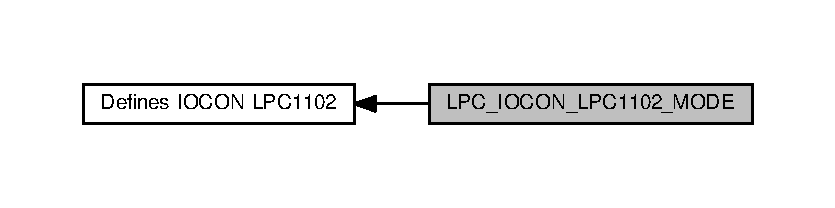
\includegraphics[width=350pt]{group___l_p_c___i_o_c_o_n___l_p_c1102___m_o_d_e}
\end{center}
\end{figure}
\subsection*{Macros}
\begin{DoxyCompactItemize}
\item 
\#define \hyperlink{group___l_p_c___i_o_c_o_n___l_p_c1102___m_o_d_e_gac0cfc0275160b96c647fc5774f34b390}{L\+P\+C\+\_\+\+I\+O\+C\+O\+N\+\_\+\+M\+O\+D\+E\+\_\+\+I\+N\+A\+C\+T\+I\+VE}~(0x00000000\+U\+L) $<$$<$ L\+P\+C\+\_\+\+I\+O\+C\+O\+N\+\_\+\+M\+O\+D\+E\+\_\+\+B\+IT
\begin{DoxyCompactList}\small\item\em Inactivo \+: sin resistencia pull-\/down/pull-\/up. \end{DoxyCompactList}\item 
\#define \hyperlink{group___l_p_c___i_o_c_o_n___l_p_c1102___m_o_d_e_gac740c9895b3d9f1c49a902a7693b3ef4}{L\+P\+C\+\_\+\+I\+O\+C\+O\+N\+\_\+\+M\+O\+D\+E\+\_\+\+P\+U\+L\+L\+D\+O\+WN}~(0x00000001\+U\+L) $<$$<$ L\+P\+C\+\_\+\+I\+O\+C\+O\+N\+\_\+\+M\+O\+D\+E\+\_\+\+B\+IT
\begin{DoxyCompactList}\small\item\em Resistencia de Pull-\/\+Down habilitada. \end{DoxyCompactList}\item 
\#define \hyperlink{group___l_p_c___i_o_c_o_n___l_p_c1102___m_o_d_e_ga36c30fc68af8e4dfdda3ed4116bbb9e1}{L\+P\+C\+\_\+\+I\+O\+C\+O\+N\+\_\+\+M\+O\+D\+E\+\_\+\+P\+U\+L\+L\+UP}~(0x00000002\+U\+L) $<$$<$ L\+P\+C\+\_\+\+I\+O\+C\+O\+N\+\_\+\+M\+O\+D\+E\+\_\+\+B\+IT
\begin{DoxyCompactList}\small\item\em Resistencia de Pull-\/\+Up habilitada. \end{DoxyCompactList}\item 
\#define \hyperlink{group___l_p_c___i_o_c_o_n___l_p_c1102___m_o_d_e_ga622cda7f7867ff277096fe6ccb94d046}{L\+P\+C\+\_\+\+I\+O\+C\+O\+N\+\_\+\+M\+O\+D\+E\+\_\+\+R\+E\+P\+E\+A\+T\+ER}~(0x00000003\+U\+L) $<$$<$ L\+P\+C\+\_\+\+I\+O\+C\+O\+N\+\_\+\+M\+O\+D\+E\+\_\+\+B\+IT
\begin{DoxyCompactList}\small\item\em Modo repetidor. \end{DoxyCompactList}\end{DoxyCompactItemize}


\subsection{Detailed Description}
Modos del registro I\+O\+C\+ON comunes a todos los pines. 



\subsection{Macro Definition Documentation}
\index{L\+P\+C\+\_\+\+I\+O\+C\+O\+N\+\_\+\+L\+P\+C1102\+\_\+\+M\+O\+DE@{L\+P\+C\+\_\+\+I\+O\+C\+O\+N\+\_\+\+L\+P\+C1102\+\_\+\+M\+O\+DE}!L\+P\+C\+\_\+\+I\+O\+C\+O\+N\+\_\+\+M\+O\+D\+E\+\_\+\+I\+N\+A\+C\+T\+I\+VE@{L\+P\+C\+\_\+\+I\+O\+C\+O\+N\+\_\+\+M\+O\+D\+E\+\_\+\+I\+N\+A\+C\+T\+I\+VE}}
\index{L\+P\+C\+\_\+\+I\+O\+C\+O\+N\+\_\+\+M\+O\+D\+E\+\_\+\+I\+N\+A\+C\+T\+I\+VE@{L\+P\+C\+\_\+\+I\+O\+C\+O\+N\+\_\+\+M\+O\+D\+E\+\_\+\+I\+N\+A\+C\+T\+I\+VE}!L\+P\+C\+\_\+\+I\+O\+C\+O\+N\+\_\+\+L\+P\+C1102\+\_\+\+M\+O\+DE@{L\+P\+C\+\_\+\+I\+O\+C\+O\+N\+\_\+\+L\+P\+C1102\+\_\+\+M\+O\+DE}}
\subsubsection[{\texorpdfstring{L\+P\+C\+\_\+\+I\+O\+C\+O\+N\+\_\+\+M\+O\+D\+E\+\_\+\+I\+N\+A\+C\+T\+I\+VE}{LPC_IOCON_MODE_INACTIVE}}]{\setlength{\rightskip}{0pt plus 5cm}\#define L\+P\+C\+\_\+\+I\+O\+C\+O\+N\+\_\+\+M\+O\+D\+E\+\_\+\+I\+N\+A\+C\+T\+I\+VE~(0x00000000\+U\+L) $<$$<$ L\+P\+C\+\_\+\+I\+O\+C\+O\+N\+\_\+\+M\+O\+D\+E\+\_\+\+B\+IT}\hypertarget{group___l_p_c___i_o_c_o_n___l_p_c1102___m_o_d_e_gac0cfc0275160b96c647fc5774f34b390}{}\label{group___l_p_c___i_o_c_o_n___l_p_c1102___m_o_d_e_gac0cfc0275160b96c647fc5774f34b390}


Inactivo \+: sin resistencia pull-\/down/pull-\/up. 



Definition at line 199 of file L\+P\+C1102\+\_\+\+I\+O\+C\+O\+N.\+h.

\index{L\+P\+C\+\_\+\+I\+O\+C\+O\+N\+\_\+\+L\+P\+C1102\+\_\+\+M\+O\+DE@{L\+P\+C\+\_\+\+I\+O\+C\+O\+N\+\_\+\+L\+P\+C1102\+\_\+\+M\+O\+DE}!L\+P\+C\+\_\+\+I\+O\+C\+O\+N\+\_\+\+M\+O\+D\+E\+\_\+\+P\+U\+L\+L\+D\+O\+WN@{L\+P\+C\+\_\+\+I\+O\+C\+O\+N\+\_\+\+M\+O\+D\+E\+\_\+\+P\+U\+L\+L\+D\+O\+WN}}
\index{L\+P\+C\+\_\+\+I\+O\+C\+O\+N\+\_\+\+M\+O\+D\+E\+\_\+\+P\+U\+L\+L\+D\+O\+WN@{L\+P\+C\+\_\+\+I\+O\+C\+O\+N\+\_\+\+M\+O\+D\+E\+\_\+\+P\+U\+L\+L\+D\+O\+WN}!L\+P\+C\+\_\+\+I\+O\+C\+O\+N\+\_\+\+L\+P\+C1102\+\_\+\+M\+O\+DE@{L\+P\+C\+\_\+\+I\+O\+C\+O\+N\+\_\+\+L\+P\+C1102\+\_\+\+M\+O\+DE}}
\subsubsection[{\texorpdfstring{L\+P\+C\+\_\+\+I\+O\+C\+O\+N\+\_\+\+M\+O\+D\+E\+\_\+\+P\+U\+L\+L\+D\+O\+WN}{LPC_IOCON_MODE_PULLDOWN}}]{\setlength{\rightskip}{0pt plus 5cm}\#define L\+P\+C\+\_\+\+I\+O\+C\+O\+N\+\_\+\+M\+O\+D\+E\+\_\+\+P\+U\+L\+L\+D\+O\+WN~(0x00000001\+U\+L) $<$$<$ L\+P\+C\+\_\+\+I\+O\+C\+O\+N\+\_\+\+M\+O\+D\+E\+\_\+\+B\+IT}\hypertarget{group___l_p_c___i_o_c_o_n___l_p_c1102___m_o_d_e_gac740c9895b3d9f1c49a902a7693b3ef4}{}\label{group___l_p_c___i_o_c_o_n___l_p_c1102___m_o_d_e_gac740c9895b3d9f1c49a902a7693b3ef4}


Resistencia de Pull-\/\+Down habilitada. 



Definition at line 201 of file L\+P\+C1102\+\_\+\+I\+O\+C\+O\+N.\+h.

\index{L\+P\+C\+\_\+\+I\+O\+C\+O\+N\+\_\+\+L\+P\+C1102\+\_\+\+M\+O\+DE@{L\+P\+C\+\_\+\+I\+O\+C\+O\+N\+\_\+\+L\+P\+C1102\+\_\+\+M\+O\+DE}!L\+P\+C\+\_\+\+I\+O\+C\+O\+N\+\_\+\+M\+O\+D\+E\+\_\+\+P\+U\+L\+L\+UP@{L\+P\+C\+\_\+\+I\+O\+C\+O\+N\+\_\+\+M\+O\+D\+E\+\_\+\+P\+U\+L\+L\+UP}}
\index{L\+P\+C\+\_\+\+I\+O\+C\+O\+N\+\_\+\+M\+O\+D\+E\+\_\+\+P\+U\+L\+L\+UP@{L\+P\+C\+\_\+\+I\+O\+C\+O\+N\+\_\+\+M\+O\+D\+E\+\_\+\+P\+U\+L\+L\+UP}!L\+P\+C\+\_\+\+I\+O\+C\+O\+N\+\_\+\+L\+P\+C1102\+\_\+\+M\+O\+DE@{L\+P\+C\+\_\+\+I\+O\+C\+O\+N\+\_\+\+L\+P\+C1102\+\_\+\+M\+O\+DE}}
\subsubsection[{\texorpdfstring{L\+P\+C\+\_\+\+I\+O\+C\+O\+N\+\_\+\+M\+O\+D\+E\+\_\+\+P\+U\+L\+L\+UP}{LPC_IOCON_MODE_PULLUP}}]{\setlength{\rightskip}{0pt plus 5cm}\#define L\+P\+C\+\_\+\+I\+O\+C\+O\+N\+\_\+\+M\+O\+D\+E\+\_\+\+P\+U\+L\+L\+UP~(0x00000002\+U\+L) $<$$<$ L\+P\+C\+\_\+\+I\+O\+C\+O\+N\+\_\+\+M\+O\+D\+E\+\_\+\+B\+IT}\hypertarget{group___l_p_c___i_o_c_o_n___l_p_c1102___m_o_d_e_ga36c30fc68af8e4dfdda3ed4116bbb9e1}{}\label{group___l_p_c___i_o_c_o_n___l_p_c1102___m_o_d_e_ga36c30fc68af8e4dfdda3ed4116bbb9e1}


Resistencia de Pull-\/\+Up habilitada. 



Definition at line 203 of file L\+P\+C1102\+\_\+\+I\+O\+C\+O\+N.\+h.

\index{L\+P\+C\+\_\+\+I\+O\+C\+O\+N\+\_\+\+L\+P\+C1102\+\_\+\+M\+O\+DE@{L\+P\+C\+\_\+\+I\+O\+C\+O\+N\+\_\+\+L\+P\+C1102\+\_\+\+M\+O\+DE}!L\+P\+C\+\_\+\+I\+O\+C\+O\+N\+\_\+\+M\+O\+D\+E\+\_\+\+R\+E\+P\+E\+A\+T\+ER@{L\+P\+C\+\_\+\+I\+O\+C\+O\+N\+\_\+\+M\+O\+D\+E\+\_\+\+R\+E\+P\+E\+A\+T\+ER}}
\index{L\+P\+C\+\_\+\+I\+O\+C\+O\+N\+\_\+\+M\+O\+D\+E\+\_\+\+R\+E\+P\+E\+A\+T\+ER@{L\+P\+C\+\_\+\+I\+O\+C\+O\+N\+\_\+\+M\+O\+D\+E\+\_\+\+R\+E\+P\+E\+A\+T\+ER}!L\+P\+C\+\_\+\+I\+O\+C\+O\+N\+\_\+\+L\+P\+C1102\+\_\+\+M\+O\+DE@{L\+P\+C\+\_\+\+I\+O\+C\+O\+N\+\_\+\+L\+P\+C1102\+\_\+\+M\+O\+DE}}
\subsubsection[{\texorpdfstring{L\+P\+C\+\_\+\+I\+O\+C\+O\+N\+\_\+\+M\+O\+D\+E\+\_\+\+R\+E\+P\+E\+A\+T\+ER}{LPC_IOCON_MODE_REPEATER}}]{\setlength{\rightskip}{0pt plus 5cm}\#define L\+P\+C\+\_\+\+I\+O\+C\+O\+N\+\_\+\+M\+O\+D\+E\+\_\+\+R\+E\+P\+E\+A\+T\+ER~(0x00000003\+U\+L) $<$$<$ L\+P\+C\+\_\+\+I\+O\+C\+O\+N\+\_\+\+M\+O\+D\+E\+\_\+\+B\+IT}\hypertarget{group___l_p_c___i_o_c_o_n___l_p_c1102___m_o_d_e_ga622cda7f7867ff277096fe6ccb94d046}{}\label{group___l_p_c___i_o_c_o_n___l_p_c1102___m_o_d_e_ga622cda7f7867ff277096fe6ccb94d046}


Modo repetidor. 



Definition at line 205 of file L\+P\+C1102\+\_\+\+I\+O\+C\+O\+N.\+h.


\hypertarget{group___l_p_c___i_o_c_o_n___l_p_c1102___h_y_s___o_d}{}\section{L\+P\+C\+\_\+\+I\+O\+C\+O\+N\+\_\+\+L\+P\+C1102\+\_\+\+H\+Y\+S\+\_\+\+OD}
\label{group___l_p_c___i_o_c_o_n___l_p_c1102___h_y_s___o_d}\index{L\+P\+C\+\_\+\+I\+O\+C\+O\+N\+\_\+\+L\+P\+C1102\+\_\+\+H\+Y\+S\+\_\+\+OD@{L\+P\+C\+\_\+\+I\+O\+C\+O\+N\+\_\+\+L\+P\+C1102\+\_\+\+H\+Y\+S\+\_\+\+OD}}


Bits de histéresis y Open\+Drain.  


Collaboration diagram for L\+P\+C\+\_\+\+I\+O\+C\+O\+N\+\_\+\+L\+P\+C1102\+\_\+\+H\+Y\+S\+\_\+\+OD\+:\nopagebreak
\begin{figure}[H]
\begin{center}
\leavevmode
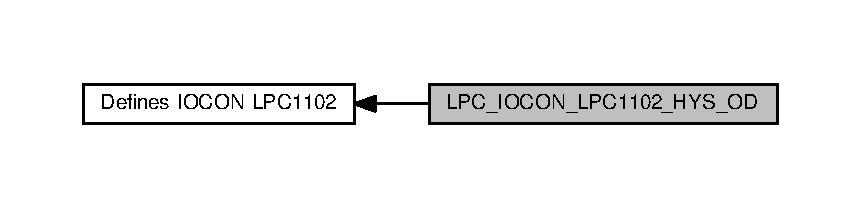
\includegraphics[width=350pt]{group___l_p_c___i_o_c_o_n___l_p_c1102___h_y_s___o_d}
\end{center}
\end{figure}
\subsection*{Bit de Histéresis}
\begin{DoxyCompactItemize}
\item 
\#define \hyperlink{group___l_p_c___i_o_c_o_n___l_p_c1102___h_y_s___o_d_ga37fea43bae0bff269cca743ebc6e9721}{L\+P\+C\+\_\+\+I\+O\+C\+O\+N\+\_\+\+H\+Y\+S\+\_\+\+D\+I\+S\+A\+B\+LE}~(0x00000000\+U\+L) $<$$<$ L\+P\+C\+\_\+\+I\+O\+C\+O\+N\+\_\+\+H\+Y\+S\+\_\+\+B\+IT
\begin{DoxyCompactList}\small\item\em Histéresis Deshabilitada. \end{DoxyCompactList}\item 
\#define \hyperlink{group___l_p_c___i_o_c_o_n___l_p_c1102___h_y_s___o_d_gafc7412adb3bb3d0a62397014fe66ed7a}{L\+P\+C\+\_\+\+I\+O\+C\+O\+N\+\_\+\+H\+Y\+S\+\_\+\+E\+N\+A\+B\+LE}~(0x00000001\+U\+L) $<$$<$ L\+P\+C\+\_\+\+I\+O\+C\+O\+N\+\_\+\+H\+Y\+S\+\_\+\+B\+IT
\begin{DoxyCompactList}\small\item\em Histéresis Habilitada. \end{DoxyCompactList}\end{DoxyCompactItemize}
\subsection*{Bit de Analog/\+Digital Mode para pines del AD}
\begin{DoxyCompactItemize}
\item 
\#define \hyperlink{group___l_p_c___i_o_c_o_n___l_p_c1102___h_y_s___o_d_gae05ef528eeed5af0eea9cc5e203a31a4}{L\+P\+C\+\_\+\+I\+O\+C\+O\+N\+\_\+\+A\+D\+M\+O\+D\+E\+\_\+\+A\+N\+A\+L\+O\+G\+\_\+\+I\+N\+P\+UT}~(0x00\+U\+L) $<$$<$ L\+P\+C\+\_\+\+I\+O\+C\+O\+N\+\_\+\+A\+D\+M\+O\+D\+E\+\_\+\+B\+IT
\begin{DoxyCompactList}\small\item\em Modo Entrada Analógica. \end{DoxyCompactList}\item 
\#define \hyperlink{group___l_p_c___i_o_c_o_n___l_p_c1102___h_y_s___o_d_ga1d822fd7d3c5e53a4f1b5e28c0592927}{L\+P\+C\+\_\+\+I\+O\+C\+O\+N\+\_\+\+A\+D\+M\+O\+D\+E\+\_\+\+D\+I\+G\+I\+T\+A\+L\+\_\+\+F\+U\+NC}~(0x01\+U\+L) $<$$<$ L\+P\+C\+\_\+\+I\+O\+C\+O\+N\+\_\+\+A\+D\+M\+O\+D\+E\+\_\+\+B\+IT
\begin{DoxyCompactList}\small\item\em Modo Función digital. \end{DoxyCompactList}\end{DoxyCompactItemize}
\subsection*{Bit de Open Drain}
\begin{DoxyCompactItemize}
\item 
\#define \hyperlink{group___l_p_c___i_o_c_o_n___l_p_c1102___h_y_s___o_d_gaf7d9ed14d2e3855efb3f6c259d67aba2}{L\+P\+C\+\_\+\+I\+O\+C\+O\+N\+\_\+\+O\+D\+\_\+\+G\+P\+I\+O\+O\+U\+T\+P\+UT}~(0x00000000\+U\+L) $<$$<$ L\+P\+C\+\_\+\+I\+O\+C\+O\+N\+\_\+\+O\+D\+\_\+\+B\+IT
\begin{DoxyCompactList}\small\item\em Salida G\+P\+IO estándar. \end{DoxyCompactList}\item 
\#define \hyperlink{group___l_p_c___i_o_c_o_n___l_p_c1102___h_y_s___o_d_ga78db812d9390dabe4c8fe7d68fc0013f}{L\+P\+C\+\_\+\+I\+O\+C\+O\+N\+\_\+\+O\+D\+\_\+\+O\+D\+O\+U\+T\+P\+UT}~(0x00000001\+U\+L) $<$$<$ L\+P\+C\+\_\+\+I\+O\+C\+O\+N\+\_\+\+O\+D\+\_\+\+B\+IT
\begin{DoxyCompactList}\small\item\em Salida Open Drain. \end{DoxyCompactList}\end{DoxyCompactItemize}


\subsection{Detailed Description}
Bits de histéresis y Open\+Drain. 



\subsection{Macro Definition Documentation}
\index{L\+P\+C\+\_\+\+I\+O\+C\+O\+N\+\_\+\+L\+P\+C1102\+\_\+\+H\+Y\+S\+\_\+\+OD@{L\+P\+C\+\_\+\+I\+O\+C\+O\+N\+\_\+\+L\+P\+C1102\+\_\+\+H\+Y\+S\+\_\+\+OD}!L\+P\+C\+\_\+\+I\+O\+C\+O\+N\+\_\+\+A\+D\+M\+O\+D\+E\+\_\+\+A\+N\+A\+L\+O\+G\+\_\+\+I\+N\+P\+UT@{L\+P\+C\+\_\+\+I\+O\+C\+O\+N\+\_\+\+A\+D\+M\+O\+D\+E\+\_\+\+A\+N\+A\+L\+O\+G\+\_\+\+I\+N\+P\+UT}}
\index{L\+P\+C\+\_\+\+I\+O\+C\+O\+N\+\_\+\+A\+D\+M\+O\+D\+E\+\_\+\+A\+N\+A\+L\+O\+G\+\_\+\+I\+N\+P\+UT@{L\+P\+C\+\_\+\+I\+O\+C\+O\+N\+\_\+\+A\+D\+M\+O\+D\+E\+\_\+\+A\+N\+A\+L\+O\+G\+\_\+\+I\+N\+P\+UT}!L\+P\+C\+\_\+\+I\+O\+C\+O\+N\+\_\+\+L\+P\+C1102\+\_\+\+H\+Y\+S\+\_\+\+OD@{L\+P\+C\+\_\+\+I\+O\+C\+O\+N\+\_\+\+L\+P\+C1102\+\_\+\+H\+Y\+S\+\_\+\+OD}}
\subsubsection[{\texorpdfstring{L\+P\+C\+\_\+\+I\+O\+C\+O\+N\+\_\+\+A\+D\+M\+O\+D\+E\+\_\+\+A\+N\+A\+L\+O\+G\+\_\+\+I\+N\+P\+UT}{LPC_IOCON_ADMODE_ANALOG_INPUT}}]{\setlength{\rightskip}{0pt plus 5cm}\#define L\+P\+C\+\_\+\+I\+O\+C\+O\+N\+\_\+\+A\+D\+M\+O\+D\+E\+\_\+\+A\+N\+A\+L\+O\+G\+\_\+\+I\+N\+P\+UT~(0x00\+U\+L) $<$$<$ L\+P\+C\+\_\+\+I\+O\+C\+O\+N\+\_\+\+A\+D\+M\+O\+D\+E\+\_\+\+B\+IT}\hypertarget{group___l_p_c___i_o_c_o_n___l_p_c1102___h_y_s___o_d_gae05ef528eeed5af0eea9cc5e203a31a4}{}\label{group___l_p_c___i_o_c_o_n___l_p_c1102___h_y_s___o_d_gae05ef528eeed5af0eea9cc5e203a31a4}


Modo Entrada Analógica. 



Definition at line 231 of file L\+P\+C1102\+\_\+\+I\+O\+C\+O\+N.\+h.

\index{L\+P\+C\+\_\+\+I\+O\+C\+O\+N\+\_\+\+L\+P\+C1102\+\_\+\+H\+Y\+S\+\_\+\+OD@{L\+P\+C\+\_\+\+I\+O\+C\+O\+N\+\_\+\+L\+P\+C1102\+\_\+\+H\+Y\+S\+\_\+\+OD}!L\+P\+C\+\_\+\+I\+O\+C\+O\+N\+\_\+\+A\+D\+M\+O\+D\+E\+\_\+\+D\+I\+G\+I\+T\+A\+L\+\_\+\+F\+U\+NC@{L\+P\+C\+\_\+\+I\+O\+C\+O\+N\+\_\+\+A\+D\+M\+O\+D\+E\+\_\+\+D\+I\+G\+I\+T\+A\+L\+\_\+\+F\+U\+NC}}
\index{L\+P\+C\+\_\+\+I\+O\+C\+O\+N\+\_\+\+A\+D\+M\+O\+D\+E\+\_\+\+D\+I\+G\+I\+T\+A\+L\+\_\+\+F\+U\+NC@{L\+P\+C\+\_\+\+I\+O\+C\+O\+N\+\_\+\+A\+D\+M\+O\+D\+E\+\_\+\+D\+I\+G\+I\+T\+A\+L\+\_\+\+F\+U\+NC}!L\+P\+C\+\_\+\+I\+O\+C\+O\+N\+\_\+\+L\+P\+C1102\+\_\+\+H\+Y\+S\+\_\+\+OD@{L\+P\+C\+\_\+\+I\+O\+C\+O\+N\+\_\+\+L\+P\+C1102\+\_\+\+H\+Y\+S\+\_\+\+OD}}
\subsubsection[{\texorpdfstring{L\+P\+C\+\_\+\+I\+O\+C\+O\+N\+\_\+\+A\+D\+M\+O\+D\+E\+\_\+\+D\+I\+G\+I\+T\+A\+L\+\_\+\+F\+U\+NC}{LPC_IOCON_ADMODE_DIGITAL_FUNC}}]{\setlength{\rightskip}{0pt plus 5cm}\#define L\+P\+C\+\_\+\+I\+O\+C\+O\+N\+\_\+\+A\+D\+M\+O\+D\+E\+\_\+\+D\+I\+G\+I\+T\+A\+L\+\_\+\+F\+U\+NC~(0x01\+U\+L) $<$$<$ L\+P\+C\+\_\+\+I\+O\+C\+O\+N\+\_\+\+A\+D\+M\+O\+D\+E\+\_\+\+B\+IT}\hypertarget{group___l_p_c___i_o_c_o_n___l_p_c1102___h_y_s___o_d_ga1d822fd7d3c5e53a4f1b5e28c0592927}{}\label{group___l_p_c___i_o_c_o_n___l_p_c1102___h_y_s___o_d_ga1d822fd7d3c5e53a4f1b5e28c0592927}


Modo Función digital. 



Definition at line 233 of file L\+P\+C1102\+\_\+\+I\+O\+C\+O\+N.\+h.

\index{L\+P\+C\+\_\+\+I\+O\+C\+O\+N\+\_\+\+L\+P\+C1102\+\_\+\+H\+Y\+S\+\_\+\+OD@{L\+P\+C\+\_\+\+I\+O\+C\+O\+N\+\_\+\+L\+P\+C1102\+\_\+\+H\+Y\+S\+\_\+\+OD}!L\+P\+C\+\_\+\+I\+O\+C\+O\+N\+\_\+\+H\+Y\+S\+\_\+\+D\+I\+S\+A\+B\+LE@{L\+P\+C\+\_\+\+I\+O\+C\+O\+N\+\_\+\+H\+Y\+S\+\_\+\+D\+I\+S\+A\+B\+LE}}
\index{L\+P\+C\+\_\+\+I\+O\+C\+O\+N\+\_\+\+H\+Y\+S\+\_\+\+D\+I\+S\+A\+B\+LE@{L\+P\+C\+\_\+\+I\+O\+C\+O\+N\+\_\+\+H\+Y\+S\+\_\+\+D\+I\+S\+A\+B\+LE}!L\+P\+C\+\_\+\+I\+O\+C\+O\+N\+\_\+\+L\+P\+C1102\+\_\+\+H\+Y\+S\+\_\+\+OD@{L\+P\+C\+\_\+\+I\+O\+C\+O\+N\+\_\+\+L\+P\+C1102\+\_\+\+H\+Y\+S\+\_\+\+OD}}
\subsubsection[{\texorpdfstring{L\+P\+C\+\_\+\+I\+O\+C\+O\+N\+\_\+\+H\+Y\+S\+\_\+\+D\+I\+S\+A\+B\+LE}{LPC_IOCON_HYS_DISABLE}}]{\setlength{\rightskip}{0pt plus 5cm}\#define L\+P\+C\+\_\+\+I\+O\+C\+O\+N\+\_\+\+H\+Y\+S\+\_\+\+D\+I\+S\+A\+B\+LE~(0x00000000\+U\+L) $<$$<$ L\+P\+C\+\_\+\+I\+O\+C\+O\+N\+\_\+\+H\+Y\+S\+\_\+\+B\+IT}\hypertarget{group___l_p_c___i_o_c_o_n___l_p_c1102___h_y_s___o_d_ga37fea43bae0bff269cca743ebc6e9721}{}\label{group___l_p_c___i_o_c_o_n___l_p_c1102___h_y_s___o_d_ga37fea43bae0bff269cca743ebc6e9721}


Histéresis Deshabilitada. 



Definition at line 221 of file L\+P\+C1102\+\_\+\+I\+O\+C\+O\+N.\+h.

\index{L\+P\+C\+\_\+\+I\+O\+C\+O\+N\+\_\+\+L\+P\+C1102\+\_\+\+H\+Y\+S\+\_\+\+OD@{L\+P\+C\+\_\+\+I\+O\+C\+O\+N\+\_\+\+L\+P\+C1102\+\_\+\+H\+Y\+S\+\_\+\+OD}!L\+P\+C\+\_\+\+I\+O\+C\+O\+N\+\_\+\+H\+Y\+S\+\_\+\+E\+N\+A\+B\+LE@{L\+P\+C\+\_\+\+I\+O\+C\+O\+N\+\_\+\+H\+Y\+S\+\_\+\+E\+N\+A\+B\+LE}}
\index{L\+P\+C\+\_\+\+I\+O\+C\+O\+N\+\_\+\+H\+Y\+S\+\_\+\+E\+N\+A\+B\+LE@{L\+P\+C\+\_\+\+I\+O\+C\+O\+N\+\_\+\+H\+Y\+S\+\_\+\+E\+N\+A\+B\+LE}!L\+P\+C\+\_\+\+I\+O\+C\+O\+N\+\_\+\+L\+P\+C1102\+\_\+\+H\+Y\+S\+\_\+\+OD@{L\+P\+C\+\_\+\+I\+O\+C\+O\+N\+\_\+\+L\+P\+C1102\+\_\+\+H\+Y\+S\+\_\+\+OD}}
\subsubsection[{\texorpdfstring{L\+P\+C\+\_\+\+I\+O\+C\+O\+N\+\_\+\+H\+Y\+S\+\_\+\+E\+N\+A\+B\+LE}{LPC_IOCON_HYS_ENABLE}}]{\setlength{\rightskip}{0pt plus 5cm}\#define L\+P\+C\+\_\+\+I\+O\+C\+O\+N\+\_\+\+H\+Y\+S\+\_\+\+E\+N\+A\+B\+LE~(0x00000001\+U\+L) $<$$<$ L\+P\+C\+\_\+\+I\+O\+C\+O\+N\+\_\+\+H\+Y\+S\+\_\+\+B\+IT}\hypertarget{group___l_p_c___i_o_c_o_n___l_p_c1102___h_y_s___o_d_gafc7412adb3bb3d0a62397014fe66ed7a}{}\label{group___l_p_c___i_o_c_o_n___l_p_c1102___h_y_s___o_d_gafc7412adb3bb3d0a62397014fe66ed7a}


Histéresis Habilitada. 



Definition at line 223 of file L\+P\+C1102\+\_\+\+I\+O\+C\+O\+N.\+h.

\index{L\+P\+C\+\_\+\+I\+O\+C\+O\+N\+\_\+\+L\+P\+C1102\+\_\+\+H\+Y\+S\+\_\+\+OD@{L\+P\+C\+\_\+\+I\+O\+C\+O\+N\+\_\+\+L\+P\+C1102\+\_\+\+H\+Y\+S\+\_\+\+OD}!L\+P\+C\+\_\+\+I\+O\+C\+O\+N\+\_\+\+O\+D\+\_\+\+G\+P\+I\+O\+O\+U\+T\+P\+UT@{L\+P\+C\+\_\+\+I\+O\+C\+O\+N\+\_\+\+O\+D\+\_\+\+G\+P\+I\+O\+O\+U\+T\+P\+UT}}
\index{L\+P\+C\+\_\+\+I\+O\+C\+O\+N\+\_\+\+O\+D\+\_\+\+G\+P\+I\+O\+O\+U\+T\+P\+UT@{L\+P\+C\+\_\+\+I\+O\+C\+O\+N\+\_\+\+O\+D\+\_\+\+G\+P\+I\+O\+O\+U\+T\+P\+UT}!L\+P\+C\+\_\+\+I\+O\+C\+O\+N\+\_\+\+L\+P\+C1102\+\_\+\+H\+Y\+S\+\_\+\+OD@{L\+P\+C\+\_\+\+I\+O\+C\+O\+N\+\_\+\+L\+P\+C1102\+\_\+\+H\+Y\+S\+\_\+\+OD}}
\subsubsection[{\texorpdfstring{L\+P\+C\+\_\+\+I\+O\+C\+O\+N\+\_\+\+O\+D\+\_\+\+G\+P\+I\+O\+O\+U\+T\+P\+UT}{LPC_IOCON_OD_GPIOOUTPUT}}]{\setlength{\rightskip}{0pt plus 5cm}\#define L\+P\+C\+\_\+\+I\+O\+C\+O\+N\+\_\+\+O\+D\+\_\+\+G\+P\+I\+O\+O\+U\+T\+P\+UT~(0x00000000\+U\+L) $<$$<$ L\+P\+C\+\_\+\+I\+O\+C\+O\+N\+\_\+\+O\+D\+\_\+\+B\+IT}\hypertarget{group___l_p_c___i_o_c_o_n___l_p_c1102___h_y_s___o_d_gaf7d9ed14d2e3855efb3f6c259d67aba2}{}\label{group___l_p_c___i_o_c_o_n___l_p_c1102___h_y_s___o_d_gaf7d9ed14d2e3855efb3f6c259d67aba2}


Salida G\+P\+IO estándar. 



Definition at line 241 of file L\+P\+C1102\+\_\+\+I\+O\+C\+O\+N.\+h.

\index{L\+P\+C\+\_\+\+I\+O\+C\+O\+N\+\_\+\+L\+P\+C1102\+\_\+\+H\+Y\+S\+\_\+\+OD@{L\+P\+C\+\_\+\+I\+O\+C\+O\+N\+\_\+\+L\+P\+C1102\+\_\+\+H\+Y\+S\+\_\+\+OD}!L\+P\+C\+\_\+\+I\+O\+C\+O\+N\+\_\+\+O\+D\+\_\+\+O\+D\+O\+U\+T\+P\+UT@{L\+P\+C\+\_\+\+I\+O\+C\+O\+N\+\_\+\+O\+D\+\_\+\+O\+D\+O\+U\+T\+P\+UT}}
\index{L\+P\+C\+\_\+\+I\+O\+C\+O\+N\+\_\+\+O\+D\+\_\+\+O\+D\+O\+U\+T\+P\+UT@{L\+P\+C\+\_\+\+I\+O\+C\+O\+N\+\_\+\+O\+D\+\_\+\+O\+D\+O\+U\+T\+P\+UT}!L\+P\+C\+\_\+\+I\+O\+C\+O\+N\+\_\+\+L\+P\+C1102\+\_\+\+H\+Y\+S\+\_\+\+OD@{L\+P\+C\+\_\+\+I\+O\+C\+O\+N\+\_\+\+L\+P\+C1102\+\_\+\+H\+Y\+S\+\_\+\+OD}}
\subsubsection[{\texorpdfstring{L\+P\+C\+\_\+\+I\+O\+C\+O\+N\+\_\+\+O\+D\+\_\+\+O\+D\+O\+U\+T\+P\+UT}{LPC_IOCON_OD_ODOUTPUT}}]{\setlength{\rightskip}{0pt plus 5cm}\#define L\+P\+C\+\_\+\+I\+O\+C\+O\+N\+\_\+\+O\+D\+\_\+\+O\+D\+O\+U\+T\+P\+UT~(0x00000001\+U\+L) $<$$<$ L\+P\+C\+\_\+\+I\+O\+C\+O\+N\+\_\+\+O\+D\+\_\+\+B\+IT}\hypertarget{group___l_p_c___i_o_c_o_n___l_p_c1102___h_y_s___o_d_ga78db812d9390dabe4c8fe7d68fc0013f}{}\label{group___l_p_c___i_o_c_o_n___l_p_c1102___h_y_s___o_d_ga78db812d9390dabe4c8fe7d68fc0013f}


Salida Open Drain. 



Definition at line 243 of file L\+P\+C1102\+\_\+\+I\+O\+C\+O\+N.\+h.


\hypertarget{group___l_p_c___i_o_c_o_n___l_p_c1102___a_s_o_c_i_a_c_i_o_n_e_s}{}\section{L\+P\+C\+\_\+\+I\+O\+C\+O\+N\+\_\+\+L\+P\+C1102\+\_\+\+A\+S\+O\+C\+I\+A\+C\+I\+O\+N\+ES}
\label{group___l_p_c___i_o_c_o_n___l_p_c1102___a_s_o_c_i_a_c_i_o_n_e_s}\index{L\+P\+C\+\_\+\+I\+O\+C\+O\+N\+\_\+\+L\+P\+C1102\+\_\+\+A\+S\+O\+C\+I\+A\+C\+I\+O\+N\+ES@{L\+P\+C\+\_\+\+I\+O\+C\+O\+N\+\_\+\+L\+P\+C1102\+\_\+\+A\+S\+O\+C\+I\+A\+C\+I\+O\+N\+ES}}


Asociacion del nombre del registro en la estructura L\+P\+C\+\_\+\+I\+O\+C\+ON con los nombres del manual de $<$letra$>$$<$nro$>$  


Collaboration diagram for L\+P\+C\+\_\+\+I\+O\+C\+O\+N\+\_\+\+L\+P\+C1102\+\_\+\+A\+S\+O\+C\+I\+A\+C\+I\+O\+N\+ES\+:\nopagebreak
\begin{figure}[H]
\begin{center}
\leavevmode
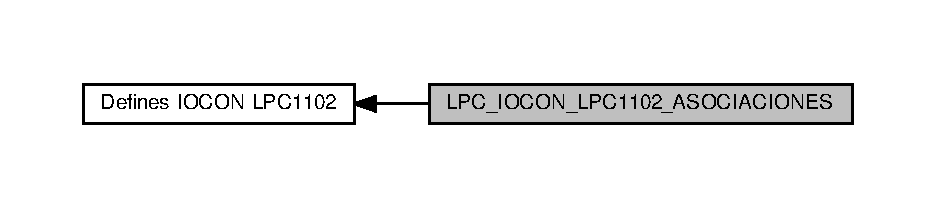
\includegraphics[width=350pt]{group___l_p_c___i_o_c_o_n___l_p_c1102___a_s_o_c_i_a_c_i_o_n_e_s}
\end{center}
\end{figure}
\subsection*{Macros}
\begin{DoxyCompactItemize}
\item 
\#define \hyperlink{group___l_p_c___i_o_c_o_n___l_p_c1102___a_s_o_c_i_a_c_i_o_n_e_s_gadf840fda55b54a90ad1ae46d4f2abe29}{L\+P\+C\+\_\+\+I\+O\+C\+O\+N\+\_\+\+C1}~\hyperlink{group___l_p_c11xx___definitions_gaabc651799ba17b0dd4a0114c8d48a145}{L\+P\+C\+\_\+\+I\+O\+C\+ON}-\/$>$R\+E\+S\+E\+T\+\_\+\+P\+I\+O0\+\_\+0
\item 
\#define \hyperlink{group___l_p_c___i_o_c_o_n___l_p_c1102___a_s_o_c_i_a_c_i_o_n_e_s_gad07b47c89c86b1b5688e116e09357df6}{L\+P\+C\+\_\+\+I\+O\+C\+O\+N\+\_\+\+A2}~\hyperlink{group___l_p_c11xx___definitions_gaabc651799ba17b0dd4a0114c8d48a145}{L\+P\+C\+\_\+\+I\+O\+C\+ON}-\/$>$P\+I\+O0\+\_\+8
\item 
\#define \hyperlink{group___l_p_c___i_o_c_o_n___l_p_c1102___a_s_o_c_i_a_c_i_o_n_e_s_ga30b8aa33fff57304e533c0a5f5a80d9a}{L\+P\+C\+\_\+\+I\+O\+C\+O\+N\+\_\+\+A3}~\hyperlink{group___l_p_c11xx___definitions_gaabc651799ba17b0dd4a0114c8d48a145}{L\+P\+C\+\_\+\+I\+O\+C\+ON}-\/$>$P\+I\+O0\+\_\+9
\item 
\#define \hyperlink{group___l_p_c___i_o_c_o_n___l_p_c1102___a_s_o_c_i_a_c_i_o_n_e_s_ga58fdb2acc1fb471de0c2e6579996c501}{L\+P\+C\+\_\+\+I\+O\+C\+O\+N\+\_\+\+A4}~\hyperlink{group___l_p_c11xx___definitions_gaabc651799ba17b0dd4a0114c8d48a145}{L\+P\+C\+\_\+\+I\+O\+C\+ON}-\/$>$S\+W\+C\+L\+K\+\_\+\+P\+I\+O0\+\_\+10
\item 
\#define \hyperlink{group___l_p_c___i_o_c_o_n___l_p_c1102___a_s_o_c_i_a_c_i_o_n_e_s_ga4a57e0dbac00d893c3aba917a8295e2d}{L\+P\+C\+\_\+\+I\+O\+C\+O\+N\+\_\+\+B4}~\hyperlink{group___l_p_c11xx___definitions_gaabc651799ba17b0dd4a0114c8d48a145}{L\+P\+C\+\_\+\+I\+O\+C\+ON}-\/$>$R\+\_\+\+P\+I\+O0\+\_\+11
\item 
\#define \hyperlink{group___l_p_c___i_o_c_o_n___l_p_c1102___a_s_o_c_i_a_c_i_o_n_e_s_gaabdb13248922a7b2c88b212a48d943b9}{L\+P\+C\+\_\+\+I\+O\+C\+O\+N\+\_\+\+B3}~\hyperlink{group___l_p_c11xx___definitions_gaabc651799ba17b0dd4a0114c8d48a145}{L\+P\+C\+\_\+\+I\+O\+C\+ON}-\/$>$R\+\_\+\+P\+I\+O1\+\_\+0
\item 
\#define \hyperlink{group___l_p_c___i_o_c_o_n___l_p_c1102___a_s_o_c_i_a_c_i_o_n_e_s_ga434a8f458a9a2656343d24444391f2c8}{L\+P\+C\+\_\+\+I\+O\+C\+O\+N\+\_\+\+C4}~\hyperlink{group___l_p_c11xx___definitions_gaabc651799ba17b0dd4a0114c8d48a145}{L\+P\+C\+\_\+\+I\+O\+C\+ON}-\/$>$R\+\_\+\+P\+I\+O1\+\_\+1
\item 
\#define \hyperlink{group___l_p_c___i_o_c_o_n___l_p_c1102___a_s_o_c_i_a_c_i_o_n_e_s_ga285291cb7f4f7bae6c08f7a6ca2885a2}{L\+P\+C\+\_\+\+I\+O\+C\+O\+N\+\_\+\+C3}~\hyperlink{group___l_p_c11xx___definitions_gaabc651799ba17b0dd4a0114c8d48a145}{L\+P\+C\+\_\+\+I\+O\+C\+ON}-\/$>$R\+\_\+\+P\+I\+O1\+\_\+2
\item 
\#define \hyperlink{group___l_p_c___i_o_c_o_n___l_p_c1102___a_s_o_c_i_a_c_i_o_n_e_s_ga25bed3139a10eb803a6e2e017fa255f9}{L\+P\+C\+\_\+\+I\+O\+C\+O\+N\+\_\+\+D4}~\hyperlink{group___l_p_c11xx___definitions_gaabc651799ba17b0dd4a0114c8d48a145}{L\+P\+C\+\_\+\+I\+O\+C\+ON}-\/$>$S\+W\+D\+I\+O\+\_\+\+P\+I\+O1\+\_\+3
\item 
\#define \hyperlink{group___l_p_c___i_o_c_o_n___l_p_c1102___a_s_o_c_i_a_c_i_o_n_e_s_ga73459d08b19f5790fa4f7514108d515b}{L\+P\+C\+\_\+\+I\+O\+C\+O\+N\+\_\+\+C2}~\hyperlink{group___l_p_c11xx___definitions_gaabc651799ba17b0dd4a0114c8d48a145}{L\+P\+C\+\_\+\+I\+O\+C\+ON}-\/$>$P\+I\+O1\+\_\+6
\item 
\#define \hyperlink{group___l_p_c___i_o_c_o_n___l_p_c1102___a_s_o_c_i_a_c_i_o_n_e_s_gae3021c481ea6e4bf372e5cd17e118f37}{L\+P\+C\+\_\+\+I\+O\+C\+O\+N\+\_\+\+D1}~\hyperlink{group___l_p_c11xx___definitions_gaabc651799ba17b0dd4a0114c8d48a145}{L\+P\+C\+\_\+\+I\+O\+C\+ON}-\/$>$P\+I\+O1\+\_\+7
\end{DoxyCompactItemize}


\subsection{Detailed Description}
Asociacion del nombre del registro en la estructura L\+P\+C\+\_\+\+I\+O\+C\+ON con los nombres del manual de $<$letra$>$$<$nro$>$ 



\subsection{Macro Definition Documentation}
\index{L\+P\+C\+\_\+\+I\+O\+C\+O\+N\+\_\+\+L\+P\+C1102\+\_\+\+A\+S\+O\+C\+I\+A\+C\+I\+O\+N\+ES@{L\+P\+C\+\_\+\+I\+O\+C\+O\+N\+\_\+\+L\+P\+C1102\+\_\+\+A\+S\+O\+C\+I\+A\+C\+I\+O\+N\+ES}!L\+P\+C\+\_\+\+I\+O\+C\+O\+N\+\_\+\+A2@{L\+P\+C\+\_\+\+I\+O\+C\+O\+N\+\_\+\+A2}}
\index{L\+P\+C\+\_\+\+I\+O\+C\+O\+N\+\_\+\+A2@{L\+P\+C\+\_\+\+I\+O\+C\+O\+N\+\_\+\+A2}!L\+P\+C\+\_\+\+I\+O\+C\+O\+N\+\_\+\+L\+P\+C1102\+\_\+\+A\+S\+O\+C\+I\+A\+C\+I\+O\+N\+ES@{L\+P\+C\+\_\+\+I\+O\+C\+O\+N\+\_\+\+L\+P\+C1102\+\_\+\+A\+S\+O\+C\+I\+A\+C\+I\+O\+N\+ES}}
\subsubsection[{\texorpdfstring{L\+P\+C\+\_\+\+I\+O\+C\+O\+N\+\_\+\+A2}{LPC_IOCON_A2}}]{\setlength{\rightskip}{0pt plus 5cm}\#define L\+P\+C\+\_\+\+I\+O\+C\+O\+N\+\_\+\+A2~{\bf L\+P\+C\+\_\+\+I\+O\+C\+ON}-\/$>$P\+I\+O0\+\_\+8}\hypertarget{group___l_p_c___i_o_c_o_n___l_p_c1102___a_s_o_c_i_a_c_i_o_n_e_s_gad07b47c89c86b1b5688e116e09357df6}{}\label{group___l_p_c___i_o_c_o_n___l_p_c1102___a_s_o_c_i_a_c_i_o_n_e_s_gad07b47c89c86b1b5688e116e09357df6}


Definition at line 257 of file L\+P\+C1102\+\_\+\+I\+O\+C\+O\+N.\+h.

\index{L\+P\+C\+\_\+\+I\+O\+C\+O\+N\+\_\+\+L\+P\+C1102\+\_\+\+A\+S\+O\+C\+I\+A\+C\+I\+O\+N\+ES@{L\+P\+C\+\_\+\+I\+O\+C\+O\+N\+\_\+\+L\+P\+C1102\+\_\+\+A\+S\+O\+C\+I\+A\+C\+I\+O\+N\+ES}!L\+P\+C\+\_\+\+I\+O\+C\+O\+N\+\_\+\+A3@{L\+P\+C\+\_\+\+I\+O\+C\+O\+N\+\_\+\+A3}}
\index{L\+P\+C\+\_\+\+I\+O\+C\+O\+N\+\_\+\+A3@{L\+P\+C\+\_\+\+I\+O\+C\+O\+N\+\_\+\+A3}!L\+P\+C\+\_\+\+I\+O\+C\+O\+N\+\_\+\+L\+P\+C1102\+\_\+\+A\+S\+O\+C\+I\+A\+C\+I\+O\+N\+ES@{L\+P\+C\+\_\+\+I\+O\+C\+O\+N\+\_\+\+L\+P\+C1102\+\_\+\+A\+S\+O\+C\+I\+A\+C\+I\+O\+N\+ES}}
\subsubsection[{\texorpdfstring{L\+P\+C\+\_\+\+I\+O\+C\+O\+N\+\_\+\+A3}{LPC_IOCON_A3}}]{\setlength{\rightskip}{0pt plus 5cm}\#define L\+P\+C\+\_\+\+I\+O\+C\+O\+N\+\_\+\+A3~{\bf L\+P\+C\+\_\+\+I\+O\+C\+ON}-\/$>$P\+I\+O0\+\_\+9}\hypertarget{group___l_p_c___i_o_c_o_n___l_p_c1102___a_s_o_c_i_a_c_i_o_n_e_s_ga30b8aa33fff57304e533c0a5f5a80d9a}{}\label{group___l_p_c___i_o_c_o_n___l_p_c1102___a_s_o_c_i_a_c_i_o_n_e_s_ga30b8aa33fff57304e533c0a5f5a80d9a}


Definition at line 258 of file L\+P\+C1102\+\_\+\+I\+O\+C\+O\+N.\+h.

\index{L\+P\+C\+\_\+\+I\+O\+C\+O\+N\+\_\+\+L\+P\+C1102\+\_\+\+A\+S\+O\+C\+I\+A\+C\+I\+O\+N\+ES@{L\+P\+C\+\_\+\+I\+O\+C\+O\+N\+\_\+\+L\+P\+C1102\+\_\+\+A\+S\+O\+C\+I\+A\+C\+I\+O\+N\+ES}!L\+P\+C\+\_\+\+I\+O\+C\+O\+N\+\_\+\+A4@{L\+P\+C\+\_\+\+I\+O\+C\+O\+N\+\_\+\+A4}}
\index{L\+P\+C\+\_\+\+I\+O\+C\+O\+N\+\_\+\+A4@{L\+P\+C\+\_\+\+I\+O\+C\+O\+N\+\_\+\+A4}!L\+P\+C\+\_\+\+I\+O\+C\+O\+N\+\_\+\+L\+P\+C1102\+\_\+\+A\+S\+O\+C\+I\+A\+C\+I\+O\+N\+ES@{L\+P\+C\+\_\+\+I\+O\+C\+O\+N\+\_\+\+L\+P\+C1102\+\_\+\+A\+S\+O\+C\+I\+A\+C\+I\+O\+N\+ES}}
\subsubsection[{\texorpdfstring{L\+P\+C\+\_\+\+I\+O\+C\+O\+N\+\_\+\+A4}{LPC_IOCON_A4}}]{\setlength{\rightskip}{0pt plus 5cm}\#define L\+P\+C\+\_\+\+I\+O\+C\+O\+N\+\_\+\+A4~{\bf L\+P\+C\+\_\+\+I\+O\+C\+ON}-\/$>$S\+W\+C\+L\+K\+\_\+\+P\+I\+O0\+\_\+10}\hypertarget{group___l_p_c___i_o_c_o_n___l_p_c1102___a_s_o_c_i_a_c_i_o_n_e_s_ga58fdb2acc1fb471de0c2e6579996c501}{}\label{group___l_p_c___i_o_c_o_n___l_p_c1102___a_s_o_c_i_a_c_i_o_n_e_s_ga58fdb2acc1fb471de0c2e6579996c501}


Definition at line 259 of file L\+P\+C1102\+\_\+\+I\+O\+C\+O\+N.\+h.

\index{L\+P\+C\+\_\+\+I\+O\+C\+O\+N\+\_\+\+L\+P\+C1102\+\_\+\+A\+S\+O\+C\+I\+A\+C\+I\+O\+N\+ES@{L\+P\+C\+\_\+\+I\+O\+C\+O\+N\+\_\+\+L\+P\+C1102\+\_\+\+A\+S\+O\+C\+I\+A\+C\+I\+O\+N\+ES}!L\+P\+C\+\_\+\+I\+O\+C\+O\+N\+\_\+\+B3@{L\+P\+C\+\_\+\+I\+O\+C\+O\+N\+\_\+\+B3}}
\index{L\+P\+C\+\_\+\+I\+O\+C\+O\+N\+\_\+\+B3@{L\+P\+C\+\_\+\+I\+O\+C\+O\+N\+\_\+\+B3}!L\+P\+C\+\_\+\+I\+O\+C\+O\+N\+\_\+\+L\+P\+C1102\+\_\+\+A\+S\+O\+C\+I\+A\+C\+I\+O\+N\+ES@{L\+P\+C\+\_\+\+I\+O\+C\+O\+N\+\_\+\+L\+P\+C1102\+\_\+\+A\+S\+O\+C\+I\+A\+C\+I\+O\+N\+ES}}
\subsubsection[{\texorpdfstring{L\+P\+C\+\_\+\+I\+O\+C\+O\+N\+\_\+\+B3}{LPC_IOCON_B3}}]{\setlength{\rightskip}{0pt plus 5cm}\#define L\+P\+C\+\_\+\+I\+O\+C\+O\+N\+\_\+\+B3~{\bf L\+P\+C\+\_\+\+I\+O\+C\+ON}-\/$>$R\+\_\+\+P\+I\+O1\+\_\+0}\hypertarget{group___l_p_c___i_o_c_o_n___l_p_c1102___a_s_o_c_i_a_c_i_o_n_e_s_gaabdb13248922a7b2c88b212a48d943b9}{}\label{group___l_p_c___i_o_c_o_n___l_p_c1102___a_s_o_c_i_a_c_i_o_n_e_s_gaabdb13248922a7b2c88b212a48d943b9}


Definition at line 261 of file L\+P\+C1102\+\_\+\+I\+O\+C\+O\+N.\+h.

\index{L\+P\+C\+\_\+\+I\+O\+C\+O\+N\+\_\+\+L\+P\+C1102\+\_\+\+A\+S\+O\+C\+I\+A\+C\+I\+O\+N\+ES@{L\+P\+C\+\_\+\+I\+O\+C\+O\+N\+\_\+\+L\+P\+C1102\+\_\+\+A\+S\+O\+C\+I\+A\+C\+I\+O\+N\+ES}!L\+P\+C\+\_\+\+I\+O\+C\+O\+N\+\_\+\+B4@{L\+P\+C\+\_\+\+I\+O\+C\+O\+N\+\_\+\+B4}}
\index{L\+P\+C\+\_\+\+I\+O\+C\+O\+N\+\_\+\+B4@{L\+P\+C\+\_\+\+I\+O\+C\+O\+N\+\_\+\+B4}!L\+P\+C\+\_\+\+I\+O\+C\+O\+N\+\_\+\+L\+P\+C1102\+\_\+\+A\+S\+O\+C\+I\+A\+C\+I\+O\+N\+ES@{L\+P\+C\+\_\+\+I\+O\+C\+O\+N\+\_\+\+L\+P\+C1102\+\_\+\+A\+S\+O\+C\+I\+A\+C\+I\+O\+N\+ES}}
\subsubsection[{\texorpdfstring{L\+P\+C\+\_\+\+I\+O\+C\+O\+N\+\_\+\+B4}{LPC_IOCON_B4}}]{\setlength{\rightskip}{0pt plus 5cm}\#define L\+P\+C\+\_\+\+I\+O\+C\+O\+N\+\_\+\+B4~{\bf L\+P\+C\+\_\+\+I\+O\+C\+ON}-\/$>$R\+\_\+\+P\+I\+O0\+\_\+11}\hypertarget{group___l_p_c___i_o_c_o_n___l_p_c1102___a_s_o_c_i_a_c_i_o_n_e_s_ga4a57e0dbac00d893c3aba917a8295e2d}{}\label{group___l_p_c___i_o_c_o_n___l_p_c1102___a_s_o_c_i_a_c_i_o_n_e_s_ga4a57e0dbac00d893c3aba917a8295e2d}


Definition at line 260 of file L\+P\+C1102\+\_\+\+I\+O\+C\+O\+N.\+h.

\index{L\+P\+C\+\_\+\+I\+O\+C\+O\+N\+\_\+\+L\+P\+C1102\+\_\+\+A\+S\+O\+C\+I\+A\+C\+I\+O\+N\+ES@{L\+P\+C\+\_\+\+I\+O\+C\+O\+N\+\_\+\+L\+P\+C1102\+\_\+\+A\+S\+O\+C\+I\+A\+C\+I\+O\+N\+ES}!L\+P\+C\+\_\+\+I\+O\+C\+O\+N\+\_\+\+C1@{L\+P\+C\+\_\+\+I\+O\+C\+O\+N\+\_\+\+C1}}
\index{L\+P\+C\+\_\+\+I\+O\+C\+O\+N\+\_\+\+C1@{L\+P\+C\+\_\+\+I\+O\+C\+O\+N\+\_\+\+C1}!L\+P\+C\+\_\+\+I\+O\+C\+O\+N\+\_\+\+L\+P\+C1102\+\_\+\+A\+S\+O\+C\+I\+A\+C\+I\+O\+N\+ES@{L\+P\+C\+\_\+\+I\+O\+C\+O\+N\+\_\+\+L\+P\+C1102\+\_\+\+A\+S\+O\+C\+I\+A\+C\+I\+O\+N\+ES}}
\subsubsection[{\texorpdfstring{L\+P\+C\+\_\+\+I\+O\+C\+O\+N\+\_\+\+C1}{LPC_IOCON_C1}}]{\setlength{\rightskip}{0pt plus 5cm}\#define L\+P\+C\+\_\+\+I\+O\+C\+O\+N\+\_\+\+C1~{\bf L\+P\+C\+\_\+\+I\+O\+C\+ON}-\/$>$R\+E\+S\+E\+T\+\_\+\+P\+I\+O0\+\_\+0}\hypertarget{group___l_p_c___i_o_c_o_n___l_p_c1102___a_s_o_c_i_a_c_i_o_n_e_s_gadf840fda55b54a90ad1ae46d4f2abe29}{}\label{group___l_p_c___i_o_c_o_n___l_p_c1102___a_s_o_c_i_a_c_i_o_n_e_s_gadf840fda55b54a90ad1ae46d4f2abe29}


Definition at line 256 of file L\+P\+C1102\+\_\+\+I\+O\+C\+O\+N.\+h.

\index{L\+P\+C\+\_\+\+I\+O\+C\+O\+N\+\_\+\+L\+P\+C1102\+\_\+\+A\+S\+O\+C\+I\+A\+C\+I\+O\+N\+ES@{L\+P\+C\+\_\+\+I\+O\+C\+O\+N\+\_\+\+L\+P\+C1102\+\_\+\+A\+S\+O\+C\+I\+A\+C\+I\+O\+N\+ES}!L\+P\+C\+\_\+\+I\+O\+C\+O\+N\+\_\+\+C2@{L\+P\+C\+\_\+\+I\+O\+C\+O\+N\+\_\+\+C2}}
\index{L\+P\+C\+\_\+\+I\+O\+C\+O\+N\+\_\+\+C2@{L\+P\+C\+\_\+\+I\+O\+C\+O\+N\+\_\+\+C2}!L\+P\+C\+\_\+\+I\+O\+C\+O\+N\+\_\+\+L\+P\+C1102\+\_\+\+A\+S\+O\+C\+I\+A\+C\+I\+O\+N\+ES@{L\+P\+C\+\_\+\+I\+O\+C\+O\+N\+\_\+\+L\+P\+C1102\+\_\+\+A\+S\+O\+C\+I\+A\+C\+I\+O\+N\+ES}}
\subsubsection[{\texorpdfstring{L\+P\+C\+\_\+\+I\+O\+C\+O\+N\+\_\+\+C2}{LPC_IOCON_C2}}]{\setlength{\rightskip}{0pt plus 5cm}\#define L\+P\+C\+\_\+\+I\+O\+C\+O\+N\+\_\+\+C2~{\bf L\+P\+C\+\_\+\+I\+O\+C\+ON}-\/$>$P\+I\+O1\+\_\+6}\hypertarget{group___l_p_c___i_o_c_o_n___l_p_c1102___a_s_o_c_i_a_c_i_o_n_e_s_ga73459d08b19f5790fa4f7514108d515b}{}\label{group___l_p_c___i_o_c_o_n___l_p_c1102___a_s_o_c_i_a_c_i_o_n_e_s_ga73459d08b19f5790fa4f7514108d515b}


Definition at line 265 of file L\+P\+C1102\+\_\+\+I\+O\+C\+O\+N.\+h.

\index{L\+P\+C\+\_\+\+I\+O\+C\+O\+N\+\_\+\+L\+P\+C1102\+\_\+\+A\+S\+O\+C\+I\+A\+C\+I\+O\+N\+ES@{L\+P\+C\+\_\+\+I\+O\+C\+O\+N\+\_\+\+L\+P\+C1102\+\_\+\+A\+S\+O\+C\+I\+A\+C\+I\+O\+N\+ES}!L\+P\+C\+\_\+\+I\+O\+C\+O\+N\+\_\+\+C3@{L\+P\+C\+\_\+\+I\+O\+C\+O\+N\+\_\+\+C3}}
\index{L\+P\+C\+\_\+\+I\+O\+C\+O\+N\+\_\+\+C3@{L\+P\+C\+\_\+\+I\+O\+C\+O\+N\+\_\+\+C3}!L\+P\+C\+\_\+\+I\+O\+C\+O\+N\+\_\+\+L\+P\+C1102\+\_\+\+A\+S\+O\+C\+I\+A\+C\+I\+O\+N\+ES@{L\+P\+C\+\_\+\+I\+O\+C\+O\+N\+\_\+\+L\+P\+C1102\+\_\+\+A\+S\+O\+C\+I\+A\+C\+I\+O\+N\+ES}}
\subsubsection[{\texorpdfstring{L\+P\+C\+\_\+\+I\+O\+C\+O\+N\+\_\+\+C3}{LPC_IOCON_C3}}]{\setlength{\rightskip}{0pt plus 5cm}\#define L\+P\+C\+\_\+\+I\+O\+C\+O\+N\+\_\+\+C3~{\bf L\+P\+C\+\_\+\+I\+O\+C\+ON}-\/$>$R\+\_\+\+P\+I\+O1\+\_\+2}\hypertarget{group___l_p_c___i_o_c_o_n___l_p_c1102___a_s_o_c_i_a_c_i_o_n_e_s_ga285291cb7f4f7bae6c08f7a6ca2885a2}{}\label{group___l_p_c___i_o_c_o_n___l_p_c1102___a_s_o_c_i_a_c_i_o_n_e_s_ga285291cb7f4f7bae6c08f7a6ca2885a2}


Definition at line 263 of file L\+P\+C1102\+\_\+\+I\+O\+C\+O\+N.\+h.

\index{L\+P\+C\+\_\+\+I\+O\+C\+O\+N\+\_\+\+L\+P\+C1102\+\_\+\+A\+S\+O\+C\+I\+A\+C\+I\+O\+N\+ES@{L\+P\+C\+\_\+\+I\+O\+C\+O\+N\+\_\+\+L\+P\+C1102\+\_\+\+A\+S\+O\+C\+I\+A\+C\+I\+O\+N\+ES}!L\+P\+C\+\_\+\+I\+O\+C\+O\+N\+\_\+\+C4@{L\+P\+C\+\_\+\+I\+O\+C\+O\+N\+\_\+\+C4}}
\index{L\+P\+C\+\_\+\+I\+O\+C\+O\+N\+\_\+\+C4@{L\+P\+C\+\_\+\+I\+O\+C\+O\+N\+\_\+\+C4}!L\+P\+C\+\_\+\+I\+O\+C\+O\+N\+\_\+\+L\+P\+C1102\+\_\+\+A\+S\+O\+C\+I\+A\+C\+I\+O\+N\+ES@{L\+P\+C\+\_\+\+I\+O\+C\+O\+N\+\_\+\+L\+P\+C1102\+\_\+\+A\+S\+O\+C\+I\+A\+C\+I\+O\+N\+ES}}
\subsubsection[{\texorpdfstring{L\+P\+C\+\_\+\+I\+O\+C\+O\+N\+\_\+\+C4}{LPC_IOCON_C4}}]{\setlength{\rightskip}{0pt plus 5cm}\#define L\+P\+C\+\_\+\+I\+O\+C\+O\+N\+\_\+\+C4~{\bf L\+P\+C\+\_\+\+I\+O\+C\+ON}-\/$>$R\+\_\+\+P\+I\+O1\+\_\+1}\hypertarget{group___l_p_c___i_o_c_o_n___l_p_c1102___a_s_o_c_i_a_c_i_o_n_e_s_ga434a8f458a9a2656343d24444391f2c8}{}\label{group___l_p_c___i_o_c_o_n___l_p_c1102___a_s_o_c_i_a_c_i_o_n_e_s_ga434a8f458a9a2656343d24444391f2c8}


Definition at line 262 of file L\+P\+C1102\+\_\+\+I\+O\+C\+O\+N.\+h.

\index{L\+P\+C\+\_\+\+I\+O\+C\+O\+N\+\_\+\+L\+P\+C1102\+\_\+\+A\+S\+O\+C\+I\+A\+C\+I\+O\+N\+ES@{L\+P\+C\+\_\+\+I\+O\+C\+O\+N\+\_\+\+L\+P\+C1102\+\_\+\+A\+S\+O\+C\+I\+A\+C\+I\+O\+N\+ES}!L\+P\+C\+\_\+\+I\+O\+C\+O\+N\+\_\+\+D1@{L\+P\+C\+\_\+\+I\+O\+C\+O\+N\+\_\+\+D1}}
\index{L\+P\+C\+\_\+\+I\+O\+C\+O\+N\+\_\+\+D1@{L\+P\+C\+\_\+\+I\+O\+C\+O\+N\+\_\+\+D1}!L\+P\+C\+\_\+\+I\+O\+C\+O\+N\+\_\+\+L\+P\+C1102\+\_\+\+A\+S\+O\+C\+I\+A\+C\+I\+O\+N\+ES@{L\+P\+C\+\_\+\+I\+O\+C\+O\+N\+\_\+\+L\+P\+C1102\+\_\+\+A\+S\+O\+C\+I\+A\+C\+I\+O\+N\+ES}}
\subsubsection[{\texorpdfstring{L\+P\+C\+\_\+\+I\+O\+C\+O\+N\+\_\+\+D1}{LPC_IOCON_D1}}]{\setlength{\rightskip}{0pt plus 5cm}\#define L\+P\+C\+\_\+\+I\+O\+C\+O\+N\+\_\+\+D1~{\bf L\+P\+C\+\_\+\+I\+O\+C\+ON}-\/$>$P\+I\+O1\+\_\+7}\hypertarget{group___l_p_c___i_o_c_o_n___l_p_c1102___a_s_o_c_i_a_c_i_o_n_e_s_gae3021c481ea6e4bf372e5cd17e118f37}{}\label{group___l_p_c___i_o_c_o_n___l_p_c1102___a_s_o_c_i_a_c_i_o_n_e_s_gae3021c481ea6e4bf372e5cd17e118f37}


Definition at line 266 of file L\+P\+C1102\+\_\+\+I\+O\+C\+O\+N.\+h.

\index{L\+P\+C\+\_\+\+I\+O\+C\+O\+N\+\_\+\+L\+P\+C1102\+\_\+\+A\+S\+O\+C\+I\+A\+C\+I\+O\+N\+ES@{L\+P\+C\+\_\+\+I\+O\+C\+O\+N\+\_\+\+L\+P\+C1102\+\_\+\+A\+S\+O\+C\+I\+A\+C\+I\+O\+N\+ES}!L\+P\+C\+\_\+\+I\+O\+C\+O\+N\+\_\+\+D4@{L\+P\+C\+\_\+\+I\+O\+C\+O\+N\+\_\+\+D4}}
\index{L\+P\+C\+\_\+\+I\+O\+C\+O\+N\+\_\+\+D4@{L\+P\+C\+\_\+\+I\+O\+C\+O\+N\+\_\+\+D4}!L\+P\+C\+\_\+\+I\+O\+C\+O\+N\+\_\+\+L\+P\+C1102\+\_\+\+A\+S\+O\+C\+I\+A\+C\+I\+O\+N\+ES@{L\+P\+C\+\_\+\+I\+O\+C\+O\+N\+\_\+\+L\+P\+C1102\+\_\+\+A\+S\+O\+C\+I\+A\+C\+I\+O\+N\+ES}}
\subsubsection[{\texorpdfstring{L\+P\+C\+\_\+\+I\+O\+C\+O\+N\+\_\+\+D4}{LPC_IOCON_D4}}]{\setlength{\rightskip}{0pt plus 5cm}\#define L\+P\+C\+\_\+\+I\+O\+C\+O\+N\+\_\+\+D4~{\bf L\+P\+C\+\_\+\+I\+O\+C\+ON}-\/$>$S\+W\+D\+I\+O\+\_\+\+P\+I\+O1\+\_\+3}\hypertarget{group___l_p_c___i_o_c_o_n___l_p_c1102___a_s_o_c_i_a_c_i_o_n_e_s_ga25bed3139a10eb803a6e2e017fa255f9}{}\label{group___l_p_c___i_o_c_o_n___l_p_c1102___a_s_o_c_i_a_c_i_o_n_e_s_ga25bed3139a10eb803a6e2e017fa255f9}


Definition at line 264 of file L\+P\+C1102\+\_\+\+I\+O\+C\+O\+N.\+h.


\hypertarget{group___l_p_c___i_o_c_o_n___l_p_c1102___s_c_k___l_o_c}{}\section{L\+P\+C\+\_\+\+I\+O\+C\+O\+N\+\_\+\+L\+P\+C1102\+\_\+\+S\+C\+K\+\_\+\+L\+OC}
\label{group___l_p_c___i_o_c_o_n___l_p_c1102___s_c_k___l_o_c}\index{L\+P\+C\+\_\+\+I\+O\+C\+O\+N\+\_\+\+L\+P\+C1102\+\_\+\+S\+C\+K\+\_\+\+L\+OC@{L\+P\+C\+\_\+\+I\+O\+C\+O\+N\+\_\+\+L\+P\+C1102\+\_\+\+S\+C\+K\+\_\+\+L\+OC}}


Registro que define en qué pin se asocia la función S\+CK.  


Collaboration diagram for L\+P\+C\+\_\+\+I\+O\+C\+O\+N\+\_\+\+L\+P\+C1102\+\_\+\+S\+C\+K\+\_\+\+L\+OC\+:\nopagebreak
\begin{figure}[H]
\begin{center}
\leavevmode
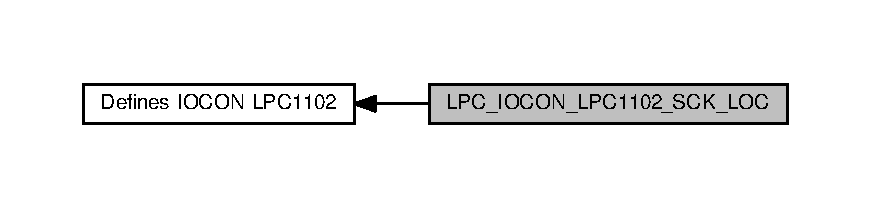
\includegraphics[width=350pt]{group___l_p_c___i_o_c_o_n___l_p_c1102___s_c_k___l_o_c}
\end{center}
\end{figure}
\subsection*{Macros}
\begin{DoxyCompactItemize}
\item 
\#define \hyperlink{group___l_p_c___i_o_c_o_n___l_p_c1102___s_c_k___l_o_c_ga831c058cf3b0a147b5833bfac8ddce82}{L\+P\+C\+\_\+\+I\+O\+C\+O\+N\+\_\+\+S\+C\+K\+L\+O\+C\+\_\+\+B\+IT}~(0)
\begin{DoxyCompactList}\small\item\em Bit del registro para modificar el pin S\+C\+K\+L\+OC. \end{DoxyCompactList}\item 
\#define \hyperlink{group___l_p_c___i_o_c_o_n___l_p_c1102___s_c_k___l_o_c_gaba2d4230db5fd5477c8f1bd850d90963}{L\+P\+C\+\_\+\+I\+O\+C\+O\+N\+\_\+\+S\+C\+K\+L\+O\+C\+\_\+\+P0\+\_\+10}~(0x00000000\+U\+L) $<$$<$ L\+P\+C\+\_\+\+I\+O\+C\+O\+N\+\_\+\+S\+C\+K\+L\+O\+C\+\_\+\+B\+IT
\begin{DoxyCompactList}\small\item\em Asocio la función de S\+CK al Pin P0.\+10 A4 (por default en L\+P\+C1102) \end{DoxyCompactList}\item 
\#define \hyperlink{group___l_p_c___i_o_c_o_n___l_p_c1102___s_c_k___l_o_c_gaa6d2e11946beb81a3e4260e789fe67fe}{L\+P\+C\+\_\+\+I\+O\+C\+O\+N\+\_\+\+S\+C\+K\+L\+O\+C\+\_\+\+P0\+\_\+6}~(0x00000002\+U\+L) $<$$<$ L\+P\+C\+\_\+\+I\+O\+C\+O\+N\+\_\+\+S\+C\+K\+L\+O\+C\+\_\+\+B\+IT
\begin{DoxyCompactList}\small\item\em Asocio la función de S\+CK al Pin P0.\+6 A1 solo en L\+P\+C1104. \end{DoxyCompactList}\end{DoxyCompactItemize}


\subsection{Detailed Description}
Registro que define en qué pin se asocia la función S\+CK. 

Para el L\+P\+C1102 solo se usaria en el valor por reset 

\subsection{Macro Definition Documentation}
\index{L\+P\+C\+\_\+\+I\+O\+C\+O\+N\+\_\+\+L\+P\+C1102\+\_\+\+S\+C\+K\+\_\+\+L\+OC@{L\+P\+C\+\_\+\+I\+O\+C\+O\+N\+\_\+\+L\+P\+C1102\+\_\+\+S\+C\+K\+\_\+\+L\+OC}!L\+P\+C\+\_\+\+I\+O\+C\+O\+N\+\_\+\+S\+C\+K\+L\+O\+C\+\_\+\+B\+IT@{L\+P\+C\+\_\+\+I\+O\+C\+O\+N\+\_\+\+S\+C\+K\+L\+O\+C\+\_\+\+B\+IT}}
\index{L\+P\+C\+\_\+\+I\+O\+C\+O\+N\+\_\+\+S\+C\+K\+L\+O\+C\+\_\+\+B\+IT@{L\+P\+C\+\_\+\+I\+O\+C\+O\+N\+\_\+\+S\+C\+K\+L\+O\+C\+\_\+\+B\+IT}!L\+P\+C\+\_\+\+I\+O\+C\+O\+N\+\_\+\+L\+P\+C1102\+\_\+\+S\+C\+K\+\_\+\+L\+OC@{L\+P\+C\+\_\+\+I\+O\+C\+O\+N\+\_\+\+L\+P\+C1102\+\_\+\+S\+C\+K\+\_\+\+L\+OC}}
\subsubsection[{\texorpdfstring{L\+P\+C\+\_\+\+I\+O\+C\+O\+N\+\_\+\+S\+C\+K\+L\+O\+C\+\_\+\+B\+IT}{LPC_IOCON_SCKLOC_BIT}}]{\setlength{\rightskip}{0pt plus 5cm}\#define L\+P\+C\+\_\+\+I\+O\+C\+O\+N\+\_\+\+S\+C\+K\+L\+O\+C\+\_\+\+B\+IT~(0)}\hypertarget{group___l_p_c___i_o_c_o_n___l_p_c1102___s_c_k___l_o_c_ga831c058cf3b0a147b5833bfac8ddce82}{}\label{group___l_p_c___i_o_c_o_n___l_p_c1102___s_c_k___l_o_c_ga831c058cf3b0a147b5833bfac8ddce82}


Bit del registro para modificar el pin S\+C\+K\+L\+OC. 



Definition at line 280 of file L\+P\+C1102\+\_\+\+I\+O\+C\+O\+N.\+h.

\index{L\+P\+C\+\_\+\+I\+O\+C\+O\+N\+\_\+\+L\+P\+C1102\+\_\+\+S\+C\+K\+\_\+\+L\+OC@{L\+P\+C\+\_\+\+I\+O\+C\+O\+N\+\_\+\+L\+P\+C1102\+\_\+\+S\+C\+K\+\_\+\+L\+OC}!L\+P\+C\+\_\+\+I\+O\+C\+O\+N\+\_\+\+S\+C\+K\+L\+O\+C\+\_\+\+P0\+\_\+10@{L\+P\+C\+\_\+\+I\+O\+C\+O\+N\+\_\+\+S\+C\+K\+L\+O\+C\+\_\+\+P0\+\_\+10}}
\index{L\+P\+C\+\_\+\+I\+O\+C\+O\+N\+\_\+\+S\+C\+K\+L\+O\+C\+\_\+\+P0\+\_\+10@{L\+P\+C\+\_\+\+I\+O\+C\+O\+N\+\_\+\+S\+C\+K\+L\+O\+C\+\_\+\+P0\+\_\+10}!L\+P\+C\+\_\+\+I\+O\+C\+O\+N\+\_\+\+L\+P\+C1102\+\_\+\+S\+C\+K\+\_\+\+L\+OC@{L\+P\+C\+\_\+\+I\+O\+C\+O\+N\+\_\+\+L\+P\+C1102\+\_\+\+S\+C\+K\+\_\+\+L\+OC}}
\subsubsection[{\texorpdfstring{L\+P\+C\+\_\+\+I\+O\+C\+O\+N\+\_\+\+S\+C\+K\+L\+O\+C\+\_\+\+P0\+\_\+10}{LPC_IOCON_SCKLOC_P0_10}}]{\setlength{\rightskip}{0pt plus 5cm}\#define L\+P\+C\+\_\+\+I\+O\+C\+O\+N\+\_\+\+S\+C\+K\+L\+O\+C\+\_\+\+P0\+\_\+10~(0x00000000\+U\+L) $<$$<$ L\+P\+C\+\_\+\+I\+O\+C\+O\+N\+\_\+\+S\+C\+K\+L\+O\+C\+\_\+\+B\+IT}\hypertarget{group___l_p_c___i_o_c_o_n___l_p_c1102___s_c_k___l_o_c_gaba2d4230db5fd5477c8f1bd850d90963}{}\label{group___l_p_c___i_o_c_o_n___l_p_c1102___s_c_k___l_o_c_gaba2d4230db5fd5477c8f1bd850d90963}


Asocio la función de S\+CK al Pin P0.\+10 A4 (por default en L\+P\+C1102) 



Definition at line 282 of file L\+P\+C1102\+\_\+\+I\+O\+C\+O\+N.\+h.

\index{L\+P\+C\+\_\+\+I\+O\+C\+O\+N\+\_\+\+L\+P\+C1102\+\_\+\+S\+C\+K\+\_\+\+L\+OC@{L\+P\+C\+\_\+\+I\+O\+C\+O\+N\+\_\+\+L\+P\+C1102\+\_\+\+S\+C\+K\+\_\+\+L\+OC}!L\+P\+C\+\_\+\+I\+O\+C\+O\+N\+\_\+\+S\+C\+K\+L\+O\+C\+\_\+\+P0\+\_\+6@{L\+P\+C\+\_\+\+I\+O\+C\+O\+N\+\_\+\+S\+C\+K\+L\+O\+C\+\_\+\+P0\+\_\+6}}
\index{L\+P\+C\+\_\+\+I\+O\+C\+O\+N\+\_\+\+S\+C\+K\+L\+O\+C\+\_\+\+P0\+\_\+6@{L\+P\+C\+\_\+\+I\+O\+C\+O\+N\+\_\+\+S\+C\+K\+L\+O\+C\+\_\+\+P0\+\_\+6}!L\+P\+C\+\_\+\+I\+O\+C\+O\+N\+\_\+\+L\+P\+C1102\+\_\+\+S\+C\+K\+\_\+\+L\+OC@{L\+P\+C\+\_\+\+I\+O\+C\+O\+N\+\_\+\+L\+P\+C1102\+\_\+\+S\+C\+K\+\_\+\+L\+OC}}
\subsubsection[{\texorpdfstring{L\+P\+C\+\_\+\+I\+O\+C\+O\+N\+\_\+\+S\+C\+K\+L\+O\+C\+\_\+\+P0\+\_\+6}{LPC_IOCON_SCKLOC_P0_6}}]{\setlength{\rightskip}{0pt plus 5cm}\#define L\+P\+C\+\_\+\+I\+O\+C\+O\+N\+\_\+\+S\+C\+K\+L\+O\+C\+\_\+\+P0\+\_\+6~(0x00000002\+U\+L) $<$$<$ L\+P\+C\+\_\+\+I\+O\+C\+O\+N\+\_\+\+S\+C\+K\+L\+O\+C\+\_\+\+B\+IT}\hypertarget{group___l_p_c___i_o_c_o_n___l_p_c1102___s_c_k___l_o_c_gaa6d2e11946beb81a3e4260e789fe67fe}{}\label{group___l_p_c___i_o_c_o_n___l_p_c1102___s_c_k___l_o_c_gaa6d2e11946beb81a3e4260e789fe67fe}


Asocio la función de S\+CK al Pin P0.\+6 A1 solo en L\+P\+C1104. 



Definition at line 284 of file L\+P\+C1102\+\_\+\+I\+O\+C\+O\+N.\+h.


\hypertarget{group___l_p_c11xx___definitions}{}\section{L\+P\+C11xx Definitions}
\label{group___l_p_c11xx___definitions}\index{L\+P\+C11xx Definitions@{L\+P\+C11xx Definitions}}
Collaboration diagram for L\+P\+C11xx Definitions\+:\nopagebreak
\begin{figure}[H]
\begin{center}
\leavevmode
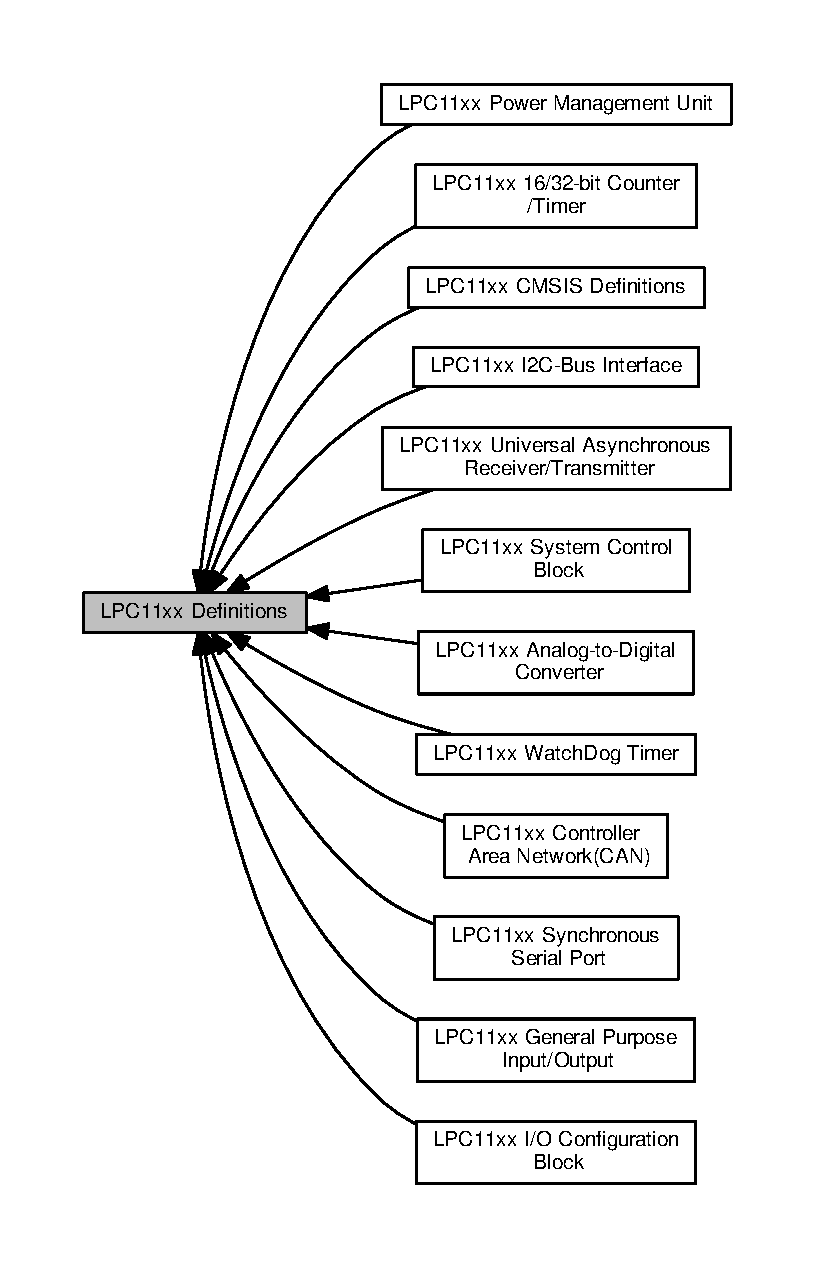
\includegraphics[width=350pt]{group___l_p_c11xx___definitions}
\end{center}
\end{figure}
\subsection*{Modules}
\begin{DoxyCompactItemize}
\item 
\hyperlink{group___l_p_c11xx___c_m_s_i_s}{L\+P\+C11xx C\+M\+S\+I\+S Definitions}
\item 
\hyperlink{group___l_p_c11xx___s_y_s_c_o_n}{L\+P\+C11xx System Control Block}
\item 
\hyperlink{group___l_p_c11xx___i_o_c_o_n}{L\+P\+C11xx I/\+O Configuration Block}
\item 
\hyperlink{group___l_p_c11xx___p_m_u}{L\+P\+C11xx Power Management Unit}
\item 
\hyperlink{group___l_p_c11xx___g_p_i_o}{L\+P\+C11xx General Purpose Input/\+Output}
\item 
\hyperlink{group___l_p_c11xx___t_m_r}{L\+P\+C11xx 16/32-\/bit Counter/\+Timer}
\item 
\hyperlink{group___l_p_c11xx___u_a_r_t}{L\+P\+C11xx Universal Asynchronous Receiver/\+Transmitter}
\item 
\hyperlink{group___l_p_c11xx___s_s_p}{L\+P\+C11xx Synchronous Serial Port}
\item 
\hyperlink{group___l_p_c11xx___i2_c}{L\+P\+C11xx I2\+C-\/\+Bus Interface}
\item 
\hyperlink{group___l_p_c11xx___w_d_t}{L\+P\+C11xx Watch\+Dog Timer}
\item 
\hyperlink{group___l_p_c11xx___a_d_c}{L\+P\+C11xx Analog-\/to-\/\+Digital Converter}
\item 
\hyperlink{group___l_p_c11xx___c_a_n}{L\+P\+C11xx Controller Area Network(\+C\+A\+N)}
\end{DoxyCompactItemize}
\subsection*{Classes}
\begin{DoxyCompactItemize}
\item 
struct \hyperlink{struct_l_p_c___f_l_a_s_h_c_t_r_l___type}{L\+P\+C\+\_\+\+F\+L\+A\+S\+H\+C\+T\+R\+L\+\_\+\+Type}
\end{DoxyCompactItemize}
\subsection*{Macros}
\begin{DoxyCompactItemize}
\item 
\#define \hyperlink{group___l_p_c11xx___definitions_ga7d7417b6cd6c6975fa03de03920d27e8}{L\+P\+C\+\_\+\+F\+L\+A\+S\+H\+\_\+\+B\+A\+SE}~(0x00000000\+U\+L)
\item 
\#define \hyperlink{group___l_p_c11xx___definitions_ga9782814ad6434f200b65440d2ac01c2a}{L\+P\+C\+\_\+\+R\+A\+M\+\_\+\+B\+A\+SE}~(0x10000000\+U\+L)
\item 
\#define \hyperlink{group___l_p_c11xx___definitions_ga55cab996c3594a0f4cc459ec8e10daea}{L\+P\+C\+\_\+\+A\+P\+B0\+\_\+\+B\+A\+SE}~(0x40000000\+U\+L)
\item 
\#define \hyperlink{group___l_p_c11xx___definitions_ga8e0d25ffe3428ed27f963e83089046a8}{L\+P\+C\+\_\+\+A\+H\+B\+\_\+\+B\+A\+SE}~(0x50000000\+U\+L)
\item 
\#define \hyperlink{group___l_p_c11xx___definitions_ga9e53652929424015ade23fe30e1d022b}{L\+P\+C\+\_\+\+I2\+C\+\_\+\+B\+A\+SE}~(\hyperlink{group___l_p_c11xx___definitions_ga55cab996c3594a0f4cc459ec8e10daea}{L\+P\+C\+\_\+\+A\+P\+B0\+\_\+\+B\+A\+SE} + 0x00000)
\item 
\#define \hyperlink{group___l_p_c11xx___definitions_ga02a30b0be4672972c3af9e5aebdcfea1}{L\+P\+C\+\_\+\+W\+D\+T\+\_\+\+B\+A\+SE}~(\hyperlink{group___l_p_c11xx___definitions_ga55cab996c3594a0f4cc459ec8e10daea}{L\+P\+C\+\_\+\+A\+P\+B0\+\_\+\+B\+A\+SE} + 0x04000)
\item 
\#define \hyperlink{group___l_p_c11xx___definitions_ga50ba023c2b0046a5be8b1b236effeb35}{L\+P\+C\+\_\+\+U\+A\+R\+T\+\_\+\+B\+A\+SE}~(\hyperlink{group___l_p_c11xx___definitions_ga55cab996c3594a0f4cc459ec8e10daea}{L\+P\+C\+\_\+\+A\+P\+B0\+\_\+\+B\+A\+SE} + 0x08000)
\item 
\#define \hyperlink{group___l_p_c11xx___definitions_ga663c7a2d9c286efce1fd9c90c0068dac}{L\+P\+C\+\_\+\+C\+T16\+B0\+\_\+\+B\+A\+SE}~(\hyperlink{group___l_p_c11xx___definitions_ga55cab996c3594a0f4cc459ec8e10daea}{L\+P\+C\+\_\+\+A\+P\+B0\+\_\+\+B\+A\+SE} + 0x0\+C000)
\item 
\#define \hyperlink{group___l_p_c11xx___definitions_ga5f33f849b010785defa0105cf6eb87f1}{L\+P\+C\+\_\+\+C\+T16\+B1\+\_\+\+B\+A\+SE}~(\hyperlink{group___l_p_c11xx___definitions_ga55cab996c3594a0f4cc459ec8e10daea}{L\+P\+C\+\_\+\+A\+P\+B0\+\_\+\+B\+A\+SE} + 0x10000)
\item 
\#define \hyperlink{group___l_p_c11xx___definitions_ga10dcc3ac224bf132010cb6bc6fc7d9c9}{L\+P\+C\+\_\+\+C\+T32\+B0\+\_\+\+B\+A\+SE}~(\hyperlink{group___l_p_c11xx___definitions_ga55cab996c3594a0f4cc459ec8e10daea}{L\+P\+C\+\_\+\+A\+P\+B0\+\_\+\+B\+A\+SE} + 0x14000)
\item 
\#define \hyperlink{group___l_p_c11xx___definitions_ga70f807832b5a2afb17265d22fed6160d}{L\+P\+C\+\_\+\+C\+T32\+B1\+\_\+\+B\+A\+SE}~(\hyperlink{group___l_p_c11xx___definitions_ga55cab996c3594a0f4cc459ec8e10daea}{L\+P\+C\+\_\+\+A\+P\+B0\+\_\+\+B\+A\+SE} + 0x18000)
\item 
\#define \hyperlink{group___l_p_c11xx___definitions_ga2396e0d0c565e4c1c3b2fc593bd6c37f}{L\+P\+C\+\_\+\+A\+D\+C\+\_\+\+B\+A\+SE}~(\hyperlink{group___l_p_c11xx___definitions_ga55cab996c3594a0f4cc459ec8e10daea}{L\+P\+C\+\_\+\+A\+P\+B0\+\_\+\+B\+A\+SE} + 0x1\+C000)
\item 
\#define \hyperlink{group___l_p_c11xx___definitions_ga865bed8ad61e9e273439ad1349a46d68}{L\+P\+C\+\_\+\+P\+M\+U\+\_\+\+B\+A\+SE}~(\hyperlink{group___l_p_c11xx___definitions_ga55cab996c3594a0f4cc459ec8e10daea}{L\+P\+C\+\_\+\+A\+P\+B0\+\_\+\+B\+A\+SE} + 0x38000)
\item 
\#define \hyperlink{group___l_p_c11xx___definitions_gad8bd09a830e15ea80293576f61deeccd}{L\+P\+C\+\_\+\+F\+L\+A\+S\+H\+C\+T\+R\+L\+\_\+\+B\+A\+SE}~(\hyperlink{group___l_p_c11xx___definitions_ga55cab996c3594a0f4cc459ec8e10daea}{L\+P\+C\+\_\+\+A\+P\+B0\+\_\+\+B\+A\+SE} + 0x3\+C000)
\item 
\#define \hyperlink{group___l_p_c11xx___definitions_ga53fb1af80b541545988f2a966681abfd}{L\+P\+C\+\_\+\+S\+S\+P0\+\_\+\+B\+A\+SE}~(\hyperlink{group___l_p_c11xx___definitions_ga55cab996c3594a0f4cc459ec8e10daea}{L\+P\+C\+\_\+\+A\+P\+B0\+\_\+\+B\+A\+SE} + 0x40000)
\item 
\#define \hyperlink{group___l_p_c11xx___definitions_gae48aea115d5924805263d7a15402d4fa}{L\+P\+C\+\_\+\+I\+O\+C\+O\+N\+\_\+\+B\+A\+SE}~(\hyperlink{group___l_p_c11xx___definitions_ga55cab996c3594a0f4cc459ec8e10daea}{L\+P\+C\+\_\+\+A\+P\+B0\+\_\+\+B\+A\+SE} + 0x44000)
\item 
\#define \hyperlink{group___l_p_c11xx___definitions_ga976cd83a81fd89a472221e68f0c0fbff}{L\+P\+C\+\_\+\+S\+Y\+S\+C\+O\+N\+\_\+\+B\+A\+SE}~(\hyperlink{group___l_p_c11xx___definitions_ga55cab996c3594a0f4cc459ec8e10daea}{L\+P\+C\+\_\+\+A\+P\+B0\+\_\+\+B\+A\+SE} + 0x48000)
\item 
\#define \hyperlink{group___l_p_c11xx___definitions_gaeae0f80f43f37b41a8a1c3cb7028d22f}{L\+P\+C\+\_\+\+C\+A\+N\+\_\+\+B\+A\+SE}~(\hyperlink{group___l_p_c11xx___definitions_ga55cab996c3594a0f4cc459ec8e10daea}{L\+P\+C\+\_\+\+A\+P\+B0\+\_\+\+B\+A\+SE} + 0x50000)
\item 
\#define \hyperlink{group___l_p_c11xx___definitions_ga05d118997f53f596d3a087f8b91a1969}{L\+P\+C\+\_\+\+S\+S\+P1\+\_\+\+B\+A\+SE}~(\hyperlink{group___l_p_c11xx___definitions_ga55cab996c3594a0f4cc459ec8e10daea}{L\+P\+C\+\_\+\+A\+P\+B0\+\_\+\+B\+A\+SE} + 0x58000)
\item 
\#define \hyperlink{group___l_p_c11xx___definitions_ga5feb4a6692784a25eaed627661bd8f36}{L\+P\+C\+\_\+\+G\+P\+I\+O\+\_\+\+B\+A\+SE}~(\hyperlink{group___l_p_c11xx___definitions_ga8e0d25ffe3428ed27f963e83089046a8}{L\+P\+C\+\_\+\+A\+H\+B\+\_\+\+B\+A\+SE}  + 0x00000)
\item 
\#define \hyperlink{group___l_p_c11xx___definitions_ga09e0e964ea1abf3b991772df2aa52405}{L\+P\+C\+\_\+\+G\+P\+I\+O0\+\_\+\+B\+A\+SE}~(\hyperlink{group___l_p_c11xx___definitions_ga8e0d25ffe3428ed27f963e83089046a8}{L\+P\+C\+\_\+\+A\+H\+B\+\_\+\+B\+A\+SE}  + 0x00000)
\item 
\#define \hyperlink{group___l_p_c11xx___definitions_ga9fb0536853721a3073bd69d94d0b7ec2}{L\+P\+C\+\_\+\+G\+P\+I\+O1\+\_\+\+B\+A\+SE}~(\hyperlink{group___l_p_c11xx___definitions_ga8e0d25ffe3428ed27f963e83089046a8}{L\+P\+C\+\_\+\+A\+H\+B\+\_\+\+B\+A\+SE}  + 0x10000)
\item 
\#define \hyperlink{group___l_p_c11xx___definitions_gae5524b2d728167194033ec7a1841a36b}{L\+P\+C\+\_\+\+G\+P\+I\+O2\+\_\+\+B\+A\+SE}~(\hyperlink{group___l_p_c11xx___definitions_ga8e0d25ffe3428ed27f963e83089046a8}{L\+P\+C\+\_\+\+A\+H\+B\+\_\+\+B\+A\+SE}  + 0x20000)
\item 
\#define \hyperlink{group___l_p_c11xx___definitions_ga56c68c5326b521b3278a35f4d81369a9}{L\+P\+C\+\_\+\+G\+P\+I\+O3\+\_\+\+B\+A\+SE}~(\hyperlink{group___l_p_c11xx___definitions_ga8e0d25ffe3428ed27f963e83089046a8}{L\+P\+C\+\_\+\+A\+H\+B\+\_\+\+B\+A\+SE}  + 0x30000)
\item 
\#define \hyperlink{group___l_p_c11xx___definitions_ga70a2faf2e119737f0e660984564d4907}{L\+P\+C\+\_\+\+I2C}~((\hyperlink{struct_l_p_c___i2_c___type_def}{L\+P\+C\+\_\+\+I2\+C\+\_\+\+Type\+Def}    $\ast$) \hyperlink{group___l_p_c11xx___definitions_ga9e53652929424015ade23fe30e1d022b}{L\+P\+C\+\_\+\+I2\+C\+\_\+\+B\+A\+SE}   )
\item 
\#define \hyperlink{group___l_p_c11xx___definitions_ga7d68cf0829652bd8c1f837c697653c5f}{L\+P\+C\+\_\+\+W\+DT}~((\hyperlink{struct_l_p_c___w_d_t___type_def}{L\+P\+C\+\_\+\+W\+D\+T\+\_\+\+Type\+Def}    $\ast$) \hyperlink{group___l_p_c11xx___definitions_ga02a30b0be4672972c3af9e5aebdcfea1}{L\+P\+C\+\_\+\+W\+D\+T\+\_\+\+B\+A\+SE}   )
\item 
\#define \hyperlink{group___l_p_c11xx___definitions_ga31a69c06776f4a82569d7ed7e91bd45c}{L\+P\+C\+\_\+\+U\+A\+RT}~((\hyperlink{struct_l_p_c___u_a_r_t___type_def}{L\+P\+C\+\_\+\+U\+A\+R\+T\+\_\+\+Type\+Def}   $\ast$) \hyperlink{group___l_p_c11xx___definitions_ga50ba023c2b0046a5be8b1b236effeb35}{L\+P\+C\+\_\+\+U\+A\+R\+T\+\_\+\+B\+A\+SE}  )
\item 
\#define \hyperlink{group___l_p_c11xx___definitions_gae3e75d39e502088028bfe901b28f6471}{L\+P\+C\+\_\+\+T\+M\+R16\+B0}~((\hyperlink{struct_l_p_c___t_m_r___type_def}{L\+P\+C\+\_\+\+T\+M\+R\+\_\+\+Type\+Def}    $\ast$) \hyperlink{group___l_p_c11xx___definitions_ga663c7a2d9c286efce1fd9c90c0068dac}{L\+P\+C\+\_\+\+C\+T16\+B0\+\_\+\+B\+A\+SE})
\item 
\#define \hyperlink{group___l_p_c11xx___definitions_gad82d36f91fa86aad5e3d57f5543e4cf6}{L\+P\+C\+\_\+\+T\+M\+R16\+B1}~((\hyperlink{struct_l_p_c___t_m_r___type_def}{L\+P\+C\+\_\+\+T\+M\+R\+\_\+\+Type\+Def}    $\ast$) \hyperlink{group___l_p_c11xx___definitions_ga5f33f849b010785defa0105cf6eb87f1}{L\+P\+C\+\_\+\+C\+T16\+B1\+\_\+\+B\+A\+SE})
\item 
\#define \hyperlink{group___l_p_c11xx___definitions_ga59694d96a23b3e6de134dc5f34ad61e8}{L\+P\+C\+\_\+\+T\+M\+R32\+B0}~((\hyperlink{struct_l_p_c___t_m_r___type_def}{L\+P\+C\+\_\+\+T\+M\+R\+\_\+\+Type\+Def}    $\ast$) \hyperlink{group___l_p_c11xx___definitions_ga10dcc3ac224bf132010cb6bc6fc7d9c9}{L\+P\+C\+\_\+\+C\+T32\+B0\+\_\+\+B\+A\+SE})
\item 
\#define \hyperlink{group___l_p_c11xx___definitions_gab5cca8bad611399aad1da65cfafcbe2e}{L\+P\+C\+\_\+\+T\+M\+R32\+B1}~((\hyperlink{struct_l_p_c___t_m_r___type_def}{L\+P\+C\+\_\+\+T\+M\+R\+\_\+\+Type\+Def}    $\ast$) \hyperlink{group___l_p_c11xx___definitions_ga70f807832b5a2afb17265d22fed6160d}{L\+P\+C\+\_\+\+C\+T32\+B1\+\_\+\+B\+A\+SE})
\item 
\#define \hyperlink{group___l_p_c11xx___definitions_gab6eaf639d3a1eec83583a9e11ab7336f}{L\+P\+C\+\_\+\+A\+DC}~((\hyperlink{struct_l_p_c___a_d_c___type_def}{L\+P\+C\+\_\+\+A\+D\+C\+\_\+\+Type\+Def}    $\ast$) \hyperlink{group___l_p_c11xx___definitions_ga2396e0d0c565e4c1c3b2fc593bd6c37f}{L\+P\+C\+\_\+\+A\+D\+C\+\_\+\+B\+A\+SE}   )
\item 
\#define \hyperlink{group___l_p_c11xx___definitions_ga9d540cc313db00679c10f9ac1961b06a}{L\+P\+C\+\_\+\+P\+MU}~((\hyperlink{struct_l_p_c___p_m_u___type_def}{L\+P\+C\+\_\+\+P\+M\+U\+\_\+\+Type\+Def}    $\ast$) \hyperlink{group___l_p_c11xx___definitions_ga865bed8ad61e9e273439ad1349a46d68}{L\+P\+C\+\_\+\+P\+M\+U\+\_\+\+B\+A\+SE}   )
\item 
\#define \hyperlink{group___l_p_c11xx___definitions_ga0e5b0ed0e4ad1155df98372c932e8bc7}{L\+P\+C\+\_\+\+F\+L\+A\+S\+H\+C\+T\+RL}~((\hyperlink{struct_l_p_c___f_l_a_s_h_c_t_r_l___type}{L\+P\+C\+\_\+\+F\+L\+A\+S\+H\+C\+T\+R\+L\+\_\+\+Type} $\ast$) \hyperlink{group___l_p_c11xx___definitions_gad8bd09a830e15ea80293576f61deeccd}{L\+P\+C\+\_\+\+F\+L\+A\+S\+H\+C\+T\+R\+L\+\_\+\+B\+A\+SE})
\item 
\#define \hyperlink{group___l_p_c11xx___definitions_gac213e0325a8e8a972bd2e0dd6ccf353c}{L\+P\+C\+\_\+\+S\+S\+P0}~((\hyperlink{struct_l_p_c___s_s_p___type_def}{L\+P\+C\+\_\+\+S\+S\+P\+\_\+\+Type\+Def}    $\ast$) \hyperlink{group___l_p_c11xx___definitions_ga53fb1af80b541545988f2a966681abfd}{L\+P\+C\+\_\+\+S\+S\+P0\+\_\+\+B\+A\+SE}  )
\item 
\#define \hyperlink{group___l_p_c11xx___definitions_ga09c4610ada1d9aa18913963cbd1a6e52}{L\+P\+C\+\_\+\+S\+S\+P1}~((\hyperlink{struct_l_p_c___s_s_p___type_def}{L\+P\+C\+\_\+\+S\+S\+P\+\_\+\+Type\+Def}    $\ast$) \hyperlink{group___l_p_c11xx___definitions_ga05d118997f53f596d3a087f8b91a1969}{L\+P\+C\+\_\+\+S\+S\+P1\+\_\+\+B\+A\+SE}  )
\item 
\#define \hyperlink{group___l_p_c11xx___definitions_ga177aa5b075c24ed459e92f4698bea9cc}{L\+P\+C\+\_\+\+C\+AN}~((\hyperlink{struct_l_p_c___c_a_n___type_def}{L\+P\+C\+\_\+\+C\+A\+N\+\_\+\+Type\+Def}    $\ast$) \hyperlink{group___l_p_c11xx___definitions_gaeae0f80f43f37b41a8a1c3cb7028d22f}{L\+P\+C\+\_\+\+C\+A\+N\+\_\+\+B\+A\+SE}   )
\item 
\#define \hyperlink{group___l_p_c11xx___definitions_gaabc651799ba17b0dd4a0114c8d48a145}{L\+P\+C\+\_\+\+I\+O\+C\+ON}~((\hyperlink{struct_l_p_c___i_o_c_o_n___type_def}{L\+P\+C\+\_\+\+I\+O\+C\+O\+N\+\_\+\+Type\+Def}  $\ast$) \hyperlink{group___l_p_c11xx___definitions_gae48aea115d5924805263d7a15402d4fa}{L\+P\+C\+\_\+\+I\+O\+C\+O\+N\+\_\+\+B\+A\+SE} )
\item 
\#define \hyperlink{group___l_p_c11xx___definitions_gabe45c10a979fe812e3d9ecd72fe33a2f}{L\+P\+C\+\_\+\+S\+Y\+S\+C\+ON}~((\hyperlink{struct_l_p_c___s_y_s_c_o_n___type_def}{L\+P\+C\+\_\+\+S\+Y\+S\+C\+O\+N\+\_\+\+Type\+Def} $\ast$) \hyperlink{group___l_p_c11xx___definitions_ga976cd83a81fd89a472221e68f0c0fbff}{L\+P\+C\+\_\+\+S\+Y\+S\+C\+O\+N\+\_\+\+B\+A\+SE})
\item 
\#define \hyperlink{group___l_p_c11xx___definitions_ga92f3de6ff5cfd5b8c290696fad07b18a}{L\+P\+C\+\_\+\+G\+P\+I\+O0}~((\hyperlink{struct_l_p_c___g_p_i_o___type_def}{L\+P\+C\+\_\+\+G\+P\+I\+O\+\_\+\+Type\+Def}   $\ast$) \hyperlink{group___l_p_c11xx___definitions_ga09e0e964ea1abf3b991772df2aa52405}{L\+P\+C\+\_\+\+G\+P\+I\+O0\+\_\+\+B\+A\+SE} )
\item 
\#define \hyperlink{group___l_p_c11xx___definitions_ga335587dad4e6d0da56c1f3ad1c087d10}{L\+P\+C\+\_\+\+G\+P\+I\+O1}~((\hyperlink{struct_l_p_c___g_p_i_o___type_def}{L\+P\+C\+\_\+\+G\+P\+I\+O\+\_\+\+Type\+Def}   $\ast$) \hyperlink{group___l_p_c11xx___definitions_ga9fb0536853721a3073bd69d94d0b7ec2}{L\+P\+C\+\_\+\+G\+P\+I\+O1\+\_\+\+B\+A\+SE} )
\item 
\#define \hyperlink{group___l_p_c11xx___definitions_ga27a09e8c08f9e209c6af70b0a3c56b39}{L\+P\+C\+\_\+\+G\+P\+I\+O2}~((\hyperlink{struct_l_p_c___g_p_i_o___type_def}{L\+P\+C\+\_\+\+G\+P\+I\+O\+\_\+\+Type\+Def}   $\ast$) \hyperlink{group___l_p_c11xx___definitions_gae5524b2d728167194033ec7a1841a36b}{L\+P\+C\+\_\+\+G\+P\+I\+O2\+\_\+\+B\+A\+SE} )
\item 
\#define \hyperlink{group___l_p_c11xx___definitions_ga6e961eb01d0f1e61dd9b9d5979d2aafc}{L\+P\+C\+\_\+\+G\+P\+I\+O3}~((\hyperlink{struct_l_p_c___g_p_i_o___type_def}{L\+P\+C\+\_\+\+G\+P\+I\+O\+\_\+\+Type\+Def}   $\ast$) \hyperlink{group___l_p_c11xx___definitions_ga56c68c5326b521b3278a35f4d81369a9}{L\+P\+C\+\_\+\+G\+P\+I\+O3\+\_\+\+B\+A\+SE} )
\end{DoxyCompactItemize}
\subsection*{Variables}
\begin{DoxyCompactItemize}
\item 
\hyperlink{group___c_m_s_i_s__core__definitions_gaec43007d9998a0a0e01faede4133d6be}{\+\_\+\+\_\+\+IO} uint32\+\_\+t \hyperlink{group___l_p_c11xx___definitions_ga970fb69752548b297feae4645834cce1}{L\+P\+C\+\_\+\+S\+Y\+S\+C\+O\+N\+\_\+\+Type\+Def\+::\+S\+Y\+S\+M\+E\+M\+R\+E\+M\+AP}
\item 
\hyperlink{group___c_m_s_i_s__core__definitions_gaec43007d9998a0a0e01faede4133d6be}{\+\_\+\+\_\+\+IO} uint32\+\_\+t \hyperlink{group___l_p_c11xx___definitions_gaf1a4b05ee430bb29acff26d16d65448d}{L\+P\+C\+\_\+\+S\+Y\+S\+C\+O\+N\+\_\+\+Type\+Def\+::\+P\+R\+E\+S\+E\+T\+C\+T\+RL}
\item 
\hyperlink{group___c_m_s_i_s__core__definitions_gaec43007d9998a0a0e01faede4133d6be}{\+\_\+\+\_\+\+IO} uint32\+\_\+t \hyperlink{group___l_p_c11xx___definitions_ga7c74ae51f98b5315c25dd045ce363f55}{L\+P\+C\+\_\+\+S\+Y\+S\+C\+O\+N\+\_\+\+Type\+Def\+::\+S\+Y\+S\+P\+L\+L\+C\+T\+RL}
\item 
\hyperlink{group___c_m_s_i_s__core__definitions_gaf63697ed9952cc71e1225efe205f6cd3}{\+\_\+\+\_\+I} uint32\+\_\+t \hyperlink{group___l_p_c11xx___definitions_gac3657072d53aa3907b0d49c252c7437f}{L\+P\+C\+\_\+\+S\+Y\+S\+C\+O\+N\+\_\+\+Type\+Def\+::\+S\+Y\+S\+P\+L\+L\+S\+T\+AT}
\item 
uint32\+\_\+t \hyperlink{group___l_p_c11xx___definitions_ga3b1f45f981b0b5c60a243403b3c158b9}{L\+P\+C\+\_\+\+S\+Y\+S\+C\+O\+N\+\_\+\+Type\+Def\+::\+R\+E\+S\+E\+R\+V\+E\+D0} \mbox{[}4\mbox{]}
\item 
\hyperlink{group___c_m_s_i_s__core__definitions_gaec43007d9998a0a0e01faede4133d6be}{\+\_\+\+\_\+\+IO} uint32\+\_\+t \hyperlink{group___l_p_c11xx___definitions_gafe759a051315e5daf1fe3d621bb72814}{L\+P\+C\+\_\+\+S\+Y\+S\+C\+O\+N\+\_\+\+Type\+Def\+::\+S\+Y\+S\+O\+S\+C\+C\+T\+RL}
\item 
\hyperlink{group___c_m_s_i_s__core__definitions_gaec43007d9998a0a0e01faede4133d6be}{\+\_\+\+\_\+\+IO} uint32\+\_\+t \hyperlink{group___l_p_c11xx___definitions_ga3ca10fa6e4f236c2f1a9dd0a801f81b3}{L\+P\+C\+\_\+\+S\+Y\+S\+C\+O\+N\+\_\+\+Type\+Def\+::\+W\+D\+T\+O\+S\+C\+C\+T\+RL}
\item 
\hyperlink{group___c_m_s_i_s__core__definitions_gaec43007d9998a0a0e01faede4133d6be}{\+\_\+\+\_\+\+IO} uint32\+\_\+t \hyperlink{group___l_p_c11xx___definitions_ga2b3e5d2e617c04cbf22c7af9070b86ee}{L\+P\+C\+\_\+\+S\+Y\+S\+C\+O\+N\+\_\+\+Type\+Def\+::\+I\+R\+C\+C\+T\+RL}
\item 
uint32\+\_\+t \hyperlink{group___l_p_c11xx___definitions_gab6f6035ebae5d3f6b21c40f152417cd2}{L\+P\+C\+\_\+\+S\+Y\+S\+C\+O\+N\+\_\+\+Type\+Def\+::\+R\+E\+S\+E\+R\+V\+E\+D1} \mbox{[}1\mbox{]}
\item 
\hyperlink{group___c_m_s_i_s__core__definitions_gaec43007d9998a0a0e01faede4133d6be}{\+\_\+\+\_\+\+IO} uint32\+\_\+t \hyperlink{group___l_p_c11xx___definitions_ga7fff308582edb9f7bfd034d3dcfde524}{L\+P\+C\+\_\+\+S\+Y\+S\+C\+O\+N\+\_\+\+Type\+Def\+::\+S\+Y\+S\+R\+S\+T\+S\+T\+AT}
\item 
uint32\+\_\+t \hyperlink{group___l_p_c11xx___definitions_gaadb6b4a71da6b8f321e2e4080864b1c1}{L\+P\+C\+\_\+\+S\+Y\+S\+C\+O\+N\+\_\+\+Type\+Def\+::\+R\+E\+S\+E\+R\+V\+E\+D2} \mbox{[}3\mbox{]}
\item 
\hyperlink{group___c_m_s_i_s__core__definitions_gaec43007d9998a0a0e01faede4133d6be}{\+\_\+\+\_\+\+IO} uint32\+\_\+t \hyperlink{group___l_p_c11xx___definitions_ga51f62077336072e5861eaf1fccebfa25}{L\+P\+C\+\_\+\+S\+Y\+S\+C\+O\+N\+\_\+\+Type\+Def\+::\+S\+Y\+S\+P\+L\+L\+C\+L\+K\+S\+EL}
\item 
\hyperlink{group___c_m_s_i_s__core__definitions_gaec43007d9998a0a0e01faede4133d6be}{\+\_\+\+\_\+\+IO} uint32\+\_\+t \hyperlink{group___l_p_c11xx___definitions_gae66518ea53c8ee53935f6a073262dab7}{L\+P\+C\+\_\+\+S\+Y\+S\+C\+O\+N\+\_\+\+Type\+Def\+::\+S\+Y\+S\+P\+L\+L\+C\+L\+K\+U\+EN}
\item 
uint32\+\_\+t \hyperlink{group___l_p_c11xx___definitions_gab166232abfe71225f9b41a1400d6ffaa}{L\+P\+C\+\_\+\+S\+Y\+S\+C\+O\+N\+\_\+\+Type\+Def\+::\+R\+E\+S\+E\+R\+V\+E\+D3} \mbox{[}10\mbox{]}
\item 
\hyperlink{group___c_m_s_i_s__core__definitions_gaec43007d9998a0a0e01faede4133d6be}{\+\_\+\+\_\+\+IO} uint32\+\_\+t \hyperlink{group___l_p_c11xx___definitions_gac54af00088fc697ce0954b04ec4786c8}{L\+P\+C\+\_\+\+S\+Y\+S\+C\+O\+N\+\_\+\+Type\+Def\+::\+M\+A\+I\+N\+C\+L\+K\+S\+EL}
\item 
\hyperlink{group___c_m_s_i_s__core__definitions_gaec43007d9998a0a0e01faede4133d6be}{\+\_\+\+\_\+\+IO} uint32\+\_\+t \hyperlink{group___l_p_c11xx___definitions_ga37489ea97331f7e125153289ab06b236}{L\+P\+C\+\_\+\+S\+Y\+S\+C\+O\+N\+\_\+\+Type\+Def\+::\+M\+A\+I\+N\+C\+L\+K\+U\+EN}
\item 
\hyperlink{group___c_m_s_i_s__core__definitions_gaec43007d9998a0a0e01faede4133d6be}{\+\_\+\+\_\+\+IO} uint32\+\_\+t \hyperlink{group___l_p_c11xx___definitions_ga2ddbe116af6e92606b3cce1ca897a4d0}{L\+P\+C\+\_\+\+S\+Y\+S\+C\+O\+N\+\_\+\+Type\+Def\+::\+S\+Y\+S\+A\+H\+B\+C\+L\+K\+D\+IV}
\item 
uint32\+\_\+t \hyperlink{group___l_p_c11xx___definitions_gadec0b128a114fba37b3501d88630acd9}{L\+P\+C\+\_\+\+S\+Y\+S\+C\+O\+N\+\_\+\+Type\+Def\+::\+R\+E\+S\+E\+R\+V\+E\+D4} \mbox{[}1\mbox{]}
\item 
\hyperlink{group___c_m_s_i_s__core__definitions_gaec43007d9998a0a0e01faede4133d6be}{\+\_\+\+\_\+\+IO} uint32\+\_\+t \hyperlink{group___l_p_c11xx___definitions_ga19b25dc1da3cf2046edafb388eeab57d}{L\+P\+C\+\_\+\+S\+Y\+S\+C\+O\+N\+\_\+\+Type\+Def\+::\+S\+Y\+S\+A\+H\+B\+C\+L\+K\+C\+T\+RL}
\item 
uint32\+\_\+t \hyperlink{group___l_p_c11xx___definitions_gac85209a97e506caccc4d0fe28f7fc63a}{L\+P\+C\+\_\+\+S\+Y\+S\+C\+O\+N\+\_\+\+Type\+Def\+::\+R\+E\+S\+E\+R\+V\+E\+D5} \mbox{[}4\mbox{]}
\item 
\hyperlink{group___c_m_s_i_s__core__definitions_gaec43007d9998a0a0e01faede4133d6be}{\+\_\+\+\_\+\+IO} uint32\+\_\+t \hyperlink{group___l_p_c11xx___definitions_gac12014d9def35fe72f78e96d151bcd2e}{L\+P\+C\+\_\+\+S\+Y\+S\+C\+O\+N\+\_\+\+Type\+Def\+::\+S\+S\+P0\+C\+L\+K\+D\+IV}
\item 
\hyperlink{group___c_m_s_i_s__core__definitions_gaec43007d9998a0a0e01faede4133d6be}{\+\_\+\+\_\+\+IO} uint32\+\_\+t \hyperlink{group___l_p_c11xx___definitions_ga5246aff7a74ac569d5a25364601e3a62}{L\+P\+C\+\_\+\+S\+Y\+S\+C\+O\+N\+\_\+\+Type\+Def\+::\+U\+A\+R\+T\+C\+L\+K\+D\+IV}
\item 
\hyperlink{group___c_m_s_i_s__core__definitions_gaec43007d9998a0a0e01faede4133d6be}{\+\_\+\+\_\+\+IO} uint32\+\_\+t \hyperlink{group___l_p_c11xx___definitions_ga0b3aeb90b3e045b2bafa727bf55fa4e0}{L\+P\+C\+\_\+\+S\+Y\+S\+C\+O\+N\+\_\+\+Type\+Def\+::\+S\+S\+P1\+C\+L\+K\+D\+IV}
\item 
uint32\+\_\+t \hyperlink{group___l_p_c11xx___definitions_ga57f21d812bc385b1452e4b634910dc96}{L\+P\+C\+\_\+\+S\+Y\+S\+C\+O\+N\+\_\+\+Type\+Def\+::\+R\+E\+S\+E\+R\+V\+E\+D6} \mbox{[}12\mbox{]}
\item 
\hyperlink{group___c_m_s_i_s__core__definitions_gaec43007d9998a0a0e01faede4133d6be}{\+\_\+\+\_\+\+IO} uint32\+\_\+t \hyperlink{group___l_p_c11xx___definitions_gafcb4b4060b3fb896d8932b4709982186}{L\+P\+C\+\_\+\+S\+Y\+S\+C\+O\+N\+\_\+\+Type\+Def\+::\+W\+D\+T\+C\+L\+K\+S\+EL}
\item 
\hyperlink{group___c_m_s_i_s__core__definitions_gaec43007d9998a0a0e01faede4133d6be}{\+\_\+\+\_\+\+IO} uint32\+\_\+t \hyperlink{group___l_p_c11xx___definitions_gafed9dd241501cd76e1f45ef74324a8c6}{L\+P\+C\+\_\+\+S\+Y\+S\+C\+O\+N\+\_\+\+Type\+Def\+::\+W\+D\+T\+C\+L\+K\+U\+EN}
\item 
\hyperlink{group___c_m_s_i_s__core__definitions_gaec43007d9998a0a0e01faede4133d6be}{\+\_\+\+\_\+\+IO} uint32\+\_\+t \hyperlink{group___l_p_c11xx___definitions_ga5d787d109526ad3eb0278790fb71a58b}{L\+P\+C\+\_\+\+S\+Y\+S\+C\+O\+N\+\_\+\+Type\+Def\+::\+W\+D\+T\+C\+L\+K\+D\+IV}
\item 
uint32\+\_\+t \hyperlink{group___l_p_c11xx___definitions_ga03a77dbffb206de6e41e18c6bc3b4895}{L\+P\+C\+\_\+\+S\+Y\+S\+C\+O\+N\+\_\+\+Type\+Def\+::\+R\+E\+S\+E\+R\+V\+E\+D8} \mbox{[}1\mbox{]}
\item 
\hyperlink{group___c_m_s_i_s__core__definitions_gaec43007d9998a0a0e01faede4133d6be}{\+\_\+\+\_\+\+IO} uint32\+\_\+t \hyperlink{group___l_p_c11xx___definitions_gac29fe890ede735895af857345a6d6cb2}{L\+P\+C\+\_\+\+S\+Y\+S\+C\+O\+N\+\_\+\+Type\+Def\+::\+C\+L\+K\+O\+U\+T\+C\+L\+K\+S\+EL}
\item 
\hyperlink{group___c_m_s_i_s__core__definitions_gaec43007d9998a0a0e01faede4133d6be}{\+\_\+\+\_\+\+IO} uint32\+\_\+t \hyperlink{group___l_p_c11xx___definitions_ga6e2e61850e73ee4ba00145e337568cdf}{L\+P\+C\+\_\+\+S\+Y\+S\+C\+O\+N\+\_\+\+Type\+Def\+::\+C\+L\+K\+O\+U\+T\+U\+EN}
\item 
\hyperlink{group___c_m_s_i_s__core__definitions_gaec43007d9998a0a0e01faede4133d6be}{\+\_\+\+\_\+\+IO} uint32\+\_\+t \hyperlink{group___l_p_c11xx___definitions_ga88ef5401531552a52e072c288d2e0900}{L\+P\+C\+\_\+\+S\+Y\+S\+C\+O\+N\+\_\+\+Type\+Def\+::\+C\+L\+K\+O\+U\+T\+D\+IV}
\item 
uint32\+\_\+t \hyperlink{group___l_p_c11xx___definitions_ga92efb41fb5e7ec4f9840b6be6d86cbaa}{L\+P\+C\+\_\+\+S\+Y\+S\+C\+O\+N\+\_\+\+Type\+Def\+::\+R\+E\+S\+E\+R\+V\+E\+D9} \mbox{[}5\mbox{]}
\item 
\hyperlink{group___c_m_s_i_s__core__definitions_gaec43007d9998a0a0e01faede4133d6be}{\+\_\+\+\_\+\+IO} uint32\+\_\+t \hyperlink{group___l_p_c11xx___definitions_gaf602252d93ac876feb330a5710324f43}{L\+P\+C\+\_\+\+S\+Y\+S\+C\+O\+N\+\_\+\+Type\+Def\+::\+P\+I\+O\+P\+O\+R\+C\+A\+P0}
\item 
\hyperlink{group___c_m_s_i_s__core__definitions_gaec43007d9998a0a0e01faede4133d6be}{\+\_\+\+\_\+\+IO} uint32\+\_\+t \hyperlink{group___l_p_c11xx___definitions_gada09efd8706154dd5e6d2675e612619f}{L\+P\+C\+\_\+\+S\+Y\+S\+C\+O\+N\+\_\+\+Type\+Def\+::\+P\+I\+O\+P\+O\+R\+C\+A\+P1}
\item 
uint32\+\_\+t \hyperlink{group___l_p_c11xx___definitions_ga60a24e7e1ad0983bd355423fd7119da7}{L\+P\+C\+\_\+\+S\+Y\+S\+C\+O\+N\+\_\+\+Type\+Def\+::\+R\+E\+S\+E\+R\+V\+E\+D10} \mbox{[}18\mbox{]}
\item 
\hyperlink{group___c_m_s_i_s__core__definitions_gaec43007d9998a0a0e01faede4133d6be}{\+\_\+\+\_\+\+IO} uint32\+\_\+t \hyperlink{group___l_p_c11xx___definitions_ga6c18e909c190b4b0819a72c6cc346661}{L\+P\+C\+\_\+\+S\+Y\+S\+C\+O\+N\+\_\+\+Type\+Def\+::\+B\+O\+D\+C\+T\+RL}
\item 
\hyperlink{group___c_m_s_i_s__core__definitions_gaec43007d9998a0a0e01faede4133d6be}{\+\_\+\+\_\+\+IO} uint32\+\_\+t \hyperlink{group___l_p_c11xx___definitions_gaa7900975ba840724314c3994379eb63b}{L\+P\+C\+\_\+\+S\+Y\+S\+C\+O\+N\+\_\+\+Type\+Def\+::\+S\+Y\+S\+T\+C\+K\+C\+AL}
\item 
uint32\+\_\+t \hyperlink{group___l_p_c11xx___definitions_ga6d48056afe2fd1921e2ce8669c3ffab7}{L\+P\+C\+\_\+\+S\+Y\+S\+C\+O\+N\+\_\+\+Type\+Def\+::\+R\+E\+S\+E\+R\+V\+E\+D13} \mbox{[}7\mbox{]}
\item 
\hyperlink{group___c_m_s_i_s__core__definitions_gaec43007d9998a0a0e01faede4133d6be}{\+\_\+\+\_\+\+IO} uint32\+\_\+t \hyperlink{group___l_p_c11xx___definitions_ga5d5f01b7f5f9ebc4067a0599113db0cd}{L\+P\+C\+\_\+\+S\+Y\+S\+C\+O\+N\+\_\+\+Type\+Def\+::\+N\+M\+I\+S\+RC}
\item 
uint32\+\_\+t \hyperlink{group___l_p_c11xx___definitions_ga044755f7a4c5447c75d2266dfe529b19}{L\+P\+C\+\_\+\+S\+Y\+S\+C\+O\+N\+\_\+\+Type\+Def\+::\+R\+E\+S\+E\+R\+V\+E\+D14} \mbox{[}34\mbox{]}
\item 
\hyperlink{group___c_m_s_i_s__core__definitions_gaec43007d9998a0a0e01faede4133d6be}{\+\_\+\+\_\+\+IO} uint32\+\_\+t \hyperlink{group___l_p_c11xx___definitions_ga2c25ccf3a127a6304bbd0cbf6b7b79d9}{L\+P\+C\+\_\+\+S\+Y\+S\+C\+O\+N\+\_\+\+Type\+Def\+::\+S\+T\+A\+R\+T\+A\+P\+R\+P0}
\item 
\hyperlink{group___c_m_s_i_s__core__definitions_gaec43007d9998a0a0e01faede4133d6be}{\+\_\+\+\_\+\+IO} uint32\+\_\+t \hyperlink{group___l_p_c11xx___definitions_ga96a994387b964d63f90460bb4d473c19}{L\+P\+C\+\_\+\+S\+Y\+S\+C\+O\+N\+\_\+\+Type\+Def\+::\+S\+T\+A\+R\+T\+E\+R\+P0}
\item 
\hyperlink{group___c_m_s_i_s__core__definitions_ga7e25d9380f9ef903923964322e71f2f6}{\+\_\+\+\_\+O} uint32\+\_\+t \hyperlink{group___l_p_c11xx___definitions_gaca777f145324363be79ee75267222aa4}{L\+P\+C\+\_\+\+S\+Y\+S\+C\+O\+N\+\_\+\+Type\+Def\+::\+S\+T\+A\+R\+T\+R\+S\+R\+P0\+C\+LR}
\item 
\hyperlink{group___c_m_s_i_s__core__definitions_gaec43007d9998a0a0e01faede4133d6be}{\+\_\+\+\_\+\+IO} uint32\+\_\+t \hyperlink{group___l_p_c11xx___definitions_ga3c4af7c32837d8f9c4f299215c6b656d}{L\+P\+C\+\_\+\+S\+Y\+S\+C\+O\+N\+\_\+\+Type\+Def\+::\+S\+T\+A\+R\+T\+S\+R\+P0}
\item 
\hyperlink{group___c_m_s_i_s__core__definitions_gaec43007d9998a0a0e01faede4133d6be}{\+\_\+\+\_\+\+IO} uint32\+\_\+t \hyperlink{group___l_p_c11xx___definitions_ga5396148c86ac74f5144944ff3a3c6eb9}{L\+P\+C\+\_\+\+S\+Y\+S\+C\+O\+N\+\_\+\+Type\+Def\+::\+S\+T\+A\+R\+T\+A\+P\+R\+P1}
\item 
\hyperlink{group___c_m_s_i_s__core__definitions_gaec43007d9998a0a0e01faede4133d6be}{\+\_\+\+\_\+\+IO} uint32\+\_\+t \hyperlink{group___l_p_c11xx___definitions_ga5965d7fdc0339537cc797fa8251f57d4}{L\+P\+C\+\_\+\+S\+Y\+S\+C\+O\+N\+\_\+\+Type\+Def\+::\+S\+T\+A\+R\+T\+E\+R\+P1}
\item 
\hyperlink{group___c_m_s_i_s__core__definitions_ga7e25d9380f9ef903923964322e71f2f6}{\+\_\+\+\_\+O} uint32\+\_\+t \hyperlink{group___l_p_c11xx___definitions_ga4cdc080e24dee708eae9cd43d9d9ea29}{L\+P\+C\+\_\+\+S\+Y\+S\+C\+O\+N\+\_\+\+Type\+Def\+::\+S\+T\+A\+R\+T\+R\+S\+R\+P1\+C\+LR}
\item 
\hyperlink{group___c_m_s_i_s__core__definitions_gaec43007d9998a0a0e01faede4133d6be}{\+\_\+\+\_\+\+IO} uint32\+\_\+t \hyperlink{group___l_p_c11xx___definitions_ga29fb26095e712d2e565e49ae4833ee4e}{L\+P\+C\+\_\+\+S\+Y\+S\+C\+O\+N\+\_\+\+Type\+Def\+::\+S\+T\+A\+R\+T\+S\+R\+P1}
\item 
uint32\+\_\+t \hyperlink{group___l_p_c11xx___definitions_ga0eb8d59fb969826b0b27b5527016d5f5}{L\+P\+C\+\_\+\+S\+Y\+S\+C\+O\+N\+\_\+\+Type\+Def\+::\+R\+E\+S\+E\+R\+V\+E\+D17} \mbox{[}4\mbox{]}
\item 
\hyperlink{group___c_m_s_i_s__core__definitions_gaec43007d9998a0a0e01faede4133d6be}{\+\_\+\+\_\+\+IO} uint32\+\_\+t \hyperlink{group___l_p_c11xx___definitions_ga6212507a2117dbb6d82fc184998e3c2c}{L\+P\+C\+\_\+\+S\+Y\+S\+C\+O\+N\+\_\+\+Type\+Def\+::\+P\+D\+S\+L\+E\+E\+P\+C\+FG}
\item 
\hyperlink{group___c_m_s_i_s__core__definitions_gaec43007d9998a0a0e01faede4133d6be}{\+\_\+\+\_\+\+IO} uint32\+\_\+t \hyperlink{group___l_p_c11xx___definitions_ga6b9a0f3442dd4f5a8a6bb8bc54236e62}{L\+P\+C\+\_\+\+S\+Y\+S\+C\+O\+N\+\_\+\+Type\+Def\+::\+P\+D\+A\+W\+A\+K\+E\+C\+FG}
\item 
\hyperlink{group___c_m_s_i_s__core__definitions_gaec43007d9998a0a0e01faede4133d6be}{\+\_\+\+\_\+\+IO} uint32\+\_\+t \hyperlink{group___l_p_c11xx___definitions_gaabb6707dad69fdc2c8eb0b10524902dd}{L\+P\+C\+\_\+\+S\+Y\+S\+C\+O\+N\+\_\+\+Type\+Def\+::\+P\+D\+R\+U\+N\+C\+FG}
\item 
uint32\+\_\+t \hyperlink{group___l_p_c11xx___definitions_gae7315f0a0ee0dc2a8e76d8bcd6f7d3cb}{L\+P\+C\+\_\+\+S\+Y\+S\+C\+O\+N\+\_\+\+Type\+Def\+::\+R\+E\+S\+E\+R\+V\+E\+D15} \mbox{[}110\mbox{]}
\item 
\hyperlink{group___c_m_s_i_s__core__definitions_gaf63697ed9952cc71e1225efe205f6cd3}{\+\_\+\+\_\+I} uint32\+\_\+t \hyperlink{group___l_p_c11xx___definitions_ga4ab05124b010cfedcc6af2f10290cb27}{L\+P\+C\+\_\+\+S\+Y\+S\+C\+O\+N\+\_\+\+Type\+Def\+::\+D\+E\+V\+I\+C\+E\+\_\+\+ID}
\item 
\hyperlink{group___c_m_s_i_s__core__definitions_gaec43007d9998a0a0e01faede4133d6be}{\+\_\+\+\_\+\+IO} uint32\+\_\+t \hyperlink{group___l_p_c11xx___definitions_gaaaca8c6a8f0ee9eadc44aefbcde5999d}{L\+P\+C\+\_\+\+I\+O\+C\+O\+N\+\_\+\+Type\+Def\+::\+P\+I\+O2\+\_\+6}
\item 
uint32\+\_\+t \hyperlink{group___l_p_c11xx___definitions_gae0c9ad1b3c2f523a2ae17423b3e14f39}{L\+P\+C\+\_\+\+I\+O\+C\+O\+N\+\_\+\+Type\+Def\+::\+R\+E\+S\+E\+R\+V\+E\+D0} \mbox{[}1\mbox{]}
\item 
\hyperlink{group___c_m_s_i_s__core__definitions_gaec43007d9998a0a0e01faede4133d6be}{\+\_\+\+\_\+\+IO} uint32\+\_\+t \hyperlink{group___l_p_c11xx___definitions_ga527d194efec901713ea175d5d735601c}{L\+P\+C\+\_\+\+I\+O\+C\+O\+N\+\_\+\+Type\+Def\+::\+P\+I\+O2\+\_\+0}
\item 
\hyperlink{group___c_m_s_i_s__core__definitions_gaec43007d9998a0a0e01faede4133d6be}{\+\_\+\+\_\+\+IO} uint32\+\_\+t \hyperlink{group___l_p_c11xx___definitions_gab69af896ceb6c10b8f9de41aa033da88}{L\+P\+C\+\_\+\+I\+O\+C\+O\+N\+\_\+\+Type\+Def\+::\+R\+E\+S\+E\+T\+\_\+\+P\+I\+O0\+\_\+0}
\item 
\hyperlink{group___c_m_s_i_s__core__definitions_gaec43007d9998a0a0e01faede4133d6be}{\+\_\+\+\_\+\+IO} uint32\+\_\+t \hyperlink{group___l_p_c11xx___definitions_ga1be433c8d0d4b04d48d7435990640b82}{L\+P\+C\+\_\+\+I\+O\+C\+O\+N\+\_\+\+Type\+Def\+::\+P\+I\+O0\+\_\+1}
\item 
\hyperlink{group___c_m_s_i_s__core__definitions_gaec43007d9998a0a0e01faede4133d6be}{\+\_\+\+\_\+\+IO} uint32\+\_\+t \hyperlink{group___l_p_c11xx___definitions_ga7b21ecfdd70f25fde6090d50447fba94}{L\+P\+C\+\_\+\+I\+O\+C\+O\+N\+\_\+\+Type\+Def\+::\+P\+I\+O1\+\_\+8}
\item 
\hyperlink{group___c_m_s_i_s__core__definitions_gaec43007d9998a0a0e01faede4133d6be}{\+\_\+\+\_\+\+IO} uint32\+\_\+t \hyperlink{group___l_p_c11xx___definitions_gade4b6c37c371658c818344930384b993}{L\+P\+C\+\_\+\+I\+O\+C\+O\+N\+\_\+\+Type\+Def\+::\+S\+S\+E\+L1\+\_\+\+L\+OC}
\item 
\hyperlink{group___c_m_s_i_s__core__definitions_gaec43007d9998a0a0e01faede4133d6be}{\+\_\+\+\_\+\+IO} uint32\+\_\+t \hyperlink{group___l_p_c11xx___definitions_ga21ff4df0d6572840ce3f9613fe1c5ef0}{L\+P\+C\+\_\+\+I\+O\+C\+O\+N\+\_\+\+Type\+Def\+::\+P\+I\+O0\+\_\+2}
\item 
\hyperlink{group___c_m_s_i_s__core__definitions_gaec43007d9998a0a0e01faede4133d6be}{\+\_\+\+\_\+\+IO} uint32\+\_\+t \hyperlink{group___l_p_c11xx___definitions_ga5c04ca957971220fb2ac40eea7aba0ff}{L\+P\+C\+\_\+\+I\+O\+C\+O\+N\+\_\+\+Type\+Def\+::\+P\+I\+O2\+\_\+7}
\item 
\hyperlink{group___c_m_s_i_s__core__definitions_gaec43007d9998a0a0e01faede4133d6be}{\+\_\+\+\_\+\+IO} uint32\+\_\+t \hyperlink{group___l_p_c11xx___definitions_gaf6abe4351486e94939abac7091e20182}{L\+P\+C\+\_\+\+I\+O\+C\+O\+N\+\_\+\+Type\+Def\+::\+P\+I\+O2\+\_\+8}
\item 
\hyperlink{group___c_m_s_i_s__core__definitions_gaec43007d9998a0a0e01faede4133d6be}{\+\_\+\+\_\+\+IO} uint32\+\_\+t \hyperlink{group___l_p_c11xx___definitions_ga8668d7e2612dde155027d1d92e4677e6}{L\+P\+C\+\_\+\+I\+O\+C\+O\+N\+\_\+\+Type\+Def\+::\+P\+I\+O2\+\_\+1}
\item 
\hyperlink{group___c_m_s_i_s__core__definitions_gaec43007d9998a0a0e01faede4133d6be}{\+\_\+\+\_\+\+IO} uint32\+\_\+t \hyperlink{group___l_p_c11xx___definitions_ga76725f15077b4abb458e593cd3ddf3c8}{L\+P\+C\+\_\+\+I\+O\+C\+O\+N\+\_\+\+Type\+Def\+::\+P\+I\+O0\+\_\+3}
\item 
\hyperlink{group___c_m_s_i_s__core__definitions_gaec43007d9998a0a0e01faede4133d6be}{\+\_\+\+\_\+\+IO} uint32\+\_\+t \hyperlink{group___l_p_c11xx___definitions_ga9c88b803f94450f62ead1a9286275696}{L\+P\+C\+\_\+\+I\+O\+C\+O\+N\+\_\+\+Type\+Def\+::\+P\+I\+O0\+\_\+4}
\item 
\hyperlink{group___c_m_s_i_s__core__definitions_gaec43007d9998a0a0e01faede4133d6be}{\+\_\+\+\_\+\+IO} uint32\+\_\+t \hyperlink{group___l_p_c11xx___definitions_ga47080726daee765a484a0788c2a99228}{L\+P\+C\+\_\+\+I\+O\+C\+O\+N\+\_\+\+Type\+Def\+::\+P\+I\+O0\+\_\+5}
\item 
\hyperlink{group___c_m_s_i_s__core__definitions_gaec43007d9998a0a0e01faede4133d6be}{\+\_\+\+\_\+\+IO} uint32\+\_\+t \hyperlink{group___l_p_c11xx___definitions_gab3da9e994b901560065126a526fae6f3}{L\+P\+C\+\_\+\+I\+O\+C\+O\+N\+\_\+\+Type\+Def\+::\+P\+I\+O1\+\_\+9}
\item 
\hyperlink{group___c_m_s_i_s__core__definitions_gaec43007d9998a0a0e01faede4133d6be}{\+\_\+\+\_\+\+IO} uint32\+\_\+t \hyperlink{group___l_p_c11xx___definitions_gac3ab46069cfc989752861c981fcd8b0a}{L\+P\+C\+\_\+\+I\+O\+C\+O\+N\+\_\+\+Type\+Def\+::\+P\+I\+O3\+\_\+4}
\item 
\hyperlink{group___c_m_s_i_s__core__definitions_gaec43007d9998a0a0e01faede4133d6be}{\+\_\+\+\_\+\+IO} uint32\+\_\+t \hyperlink{group___l_p_c11xx___definitions_ga740326ac07f023dc92db7f585e6ad407}{L\+P\+C\+\_\+\+I\+O\+C\+O\+N\+\_\+\+Type\+Def\+::\+P\+I\+O2\+\_\+4}
\item 
\hyperlink{group___c_m_s_i_s__core__definitions_gaec43007d9998a0a0e01faede4133d6be}{\+\_\+\+\_\+\+IO} uint32\+\_\+t \hyperlink{group___l_p_c11xx___definitions_gade2f9afaefeff5ab5dd1fbc04f968b34}{L\+P\+C\+\_\+\+I\+O\+C\+O\+N\+\_\+\+Type\+Def\+::\+P\+I\+O2\+\_\+5}
\item 
\hyperlink{group___c_m_s_i_s__core__definitions_gaec43007d9998a0a0e01faede4133d6be}{\+\_\+\+\_\+\+IO} uint32\+\_\+t \hyperlink{group___l_p_c11xx___definitions_ga979251234fed038c221e650f2ccaf8ae}{L\+P\+C\+\_\+\+I\+O\+C\+O\+N\+\_\+\+Type\+Def\+::\+P\+I\+O3\+\_\+5}
\item 
\hyperlink{group___c_m_s_i_s__core__definitions_gaec43007d9998a0a0e01faede4133d6be}{\+\_\+\+\_\+\+IO} uint32\+\_\+t \hyperlink{group___l_p_c11xx___definitions_ga614b18348a8f7b7604b3a3c0511eb073}{L\+P\+C\+\_\+\+I\+O\+C\+O\+N\+\_\+\+Type\+Def\+::\+P\+I\+O0\+\_\+6}
\item 
\hyperlink{group___c_m_s_i_s__core__definitions_gaec43007d9998a0a0e01faede4133d6be}{\+\_\+\+\_\+\+IO} uint32\+\_\+t \hyperlink{group___l_p_c11xx___definitions_gaa35ec9a2c3fd40798ab1fd51cc73f465}{L\+P\+C\+\_\+\+I\+O\+C\+O\+N\+\_\+\+Type\+Def\+::\+P\+I\+O0\+\_\+7}
\item 
\hyperlink{group___c_m_s_i_s__core__definitions_gaec43007d9998a0a0e01faede4133d6be}{\+\_\+\+\_\+\+IO} uint32\+\_\+t \hyperlink{group___l_p_c11xx___definitions_ga6ca4c8c499eb2f54c10dad6a8b05eacd}{L\+P\+C\+\_\+\+I\+O\+C\+O\+N\+\_\+\+Type\+Def\+::\+P\+I\+O2\+\_\+9}
\item 
\hyperlink{group___c_m_s_i_s__core__definitions_gaec43007d9998a0a0e01faede4133d6be}{\+\_\+\+\_\+\+IO} uint32\+\_\+t \hyperlink{group___l_p_c11xx___definitions_ga841de055f1f1ac93749884241ebd4274}{L\+P\+C\+\_\+\+I\+O\+C\+O\+N\+\_\+\+Type\+Def\+::\+P\+I\+O2\+\_\+10}
\item 
\hyperlink{group___c_m_s_i_s__core__definitions_gaec43007d9998a0a0e01faede4133d6be}{\+\_\+\+\_\+\+IO} uint32\+\_\+t \hyperlink{group___l_p_c11xx___definitions_gad8ad85518fffd1c1786fdc6940c108e5}{L\+P\+C\+\_\+\+I\+O\+C\+O\+N\+\_\+\+Type\+Def\+::\+P\+I\+O2\+\_\+2}
\item 
\hyperlink{group___c_m_s_i_s__core__definitions_gaec43007d9998a0a0e01faede4133d6be}{\+\_\+\+\_\+\+IO} uint32\+\_\+t \hyperlink{group___l_p_c11xx___definitions_gae04ee957f0c17950e8ef72345e57e455}{L\+P\+C\+\_\+\+I\+O\+C\+O\+N\+\_\+\+Type\+Def\+::\+P\+I\+O0\+\_\+8}
\item 
\hyperlink{group___c_m_s_i_s__core__definitions_gaec43007d9998a0a0e01faede4133d6be}{\+\_\+\+\_\+\+IO} uint32\+\_\+t \hyperlink{group___l_p_c11xx___definitions_ga11fe7c8feaa2ef89a0eed742da824d04}{L\+P\+C\+\_\+\+I\+O\+C\+O\+N\+\_\+\+Type\+Def\+::\+P\+I\+O0\+\_\+9}
\item 
\hyperlink{group___c_m_s_i_s__core__definitions_gaec43007d9998a0a0e01faede4133d6be}{\+\_\+\+\_\+\+IO} uint32\+\_\+t \hyperlink{group___l_p_c11xx___definitions_ga1c20cfee78e9855265f6c58d56d43086}{L\+P\+C\+\_\+\+I\+O\+C\+O\+N\+\_\+\+Type\+Def\+::\+S\+W\+C\+L\+K\+\_\+\+P\+I\+O0\+\_\+10}
\item 
\hyperlink{group___c_m_s_i_s__core__definitions_gaec43007d9998a0a0e01faede4133d6be}{\+\_\+\+\_\+\+IO} uint32\+\_\+t \hyperlink{group___l_p_c11xx___definitions_ga952de1f8b6cdc4f74c39ecc5997372dc}{L\+P\+C\+\_\+\+I\+O\+C\+O\+N\+\_\+\+Type\+Def\+::\+P\+I\+O1\+\_\+10}
\item 
\hyperlink{group___c_m_s_i_s__core__definitions_gaec43007d9998a0a0e01faede4133d6be}{\+\_\+\+\_\+\+IO} uint32\+\_\+t \hyperlink{group___l_p_c11xx___definitions_gad384ab0e4ae297786b37d2c3a874508f}{L\+P\+C\+\_\+\+I\+O\+C\+O\+N\+\_\+\+Type\+Def\+::\+P\+I\+O2\+\_\+11}
\item 
\hyperlink{group___c_m_s_i_s__core__definitions_gaec43007d9998a0a0e01faede4133d6be}{\+\_\+\+\_\+\+IO} uint32\+\_\+t \hyperlink{group___l_p_c11xx___definitions_ga217ef0df39e9b59c6633cdaf10460939}{L\+P\+C\+\_\+\+I\+O\+C\+O\+N\+\_\+\+Type\+Def\+::\+R\+\_\+\+P\+I\+O0\+\_\+11}
\item 
\hyperlink{group___c_m_s_i_s__core__definitions_gaec43007d9998a0a0e01faede4133d6be}{\+\_\+\+\_\+\+IO} uint32\+\_\+t \hyperlink{group___l_p_c11xx___definitions_gafa554ece26b1cedbb06e8def15bec47e}{L\+P\+C\+\_\+\+I\+O\+C\+O\+N\+\_\+\+Type\+Def\+::\+R\+\_\+\+P\+I\+O1\+\_\+0}
\item 
\hyperlink{group___c_m_s_i_s__core__definitions_gaec43007d9998a0a0e01faede4133d6be}{\+\_\+\+\_\+\+IO} uint32\+\_\+t \hyperlink{group___l_p_c11xx___definitions_gad6f021c3546227736e430948dc05e2c3}{L\+P\+C\+\_\+\+I\+O\+C\+O\+N\+\_\+\+Type\+Def\+::\+R\+\_\+\+P\+I\+O1\+\_\+1}
\item 
\hyperlink{group___c_m_s_i_s__core__definitions_gaec43007d9998a0a0e01faede4133d6be}{\+\_\+\+\_\+\+IO} uint32\+\_\+t \hyperlink{group___l_p_c11xx___definitions_gaaade79f615353aeb33fda16202c368fc}{L\+P\+C\+\_\+\+I\+O\+C\+O\+N\+\_\+\+Type\+Def\+::\+R\+\_\+\+P\+I\+O1\+\_\+2}
\item 
\hyperlink{group___c_m_s_i_s__core__definitions_gaec43007d9998a0a0e01faede4133d6be}{\+\_\+\+\_\+\+IO} uint32\+\_\+t \hyperlink{group___l_p_c11xx___definitions_ga2d5f8bc14da9cb94cb5d8184443ba458}{L\+P\+C\+\_\+\+I\+O\+C\+O\+N\+\_\+\+Type\+Def\+::\+P\+I\+O3\+\_\+0}
\item 
\hyperlink{group___c_m_s_i_s__core__definitions_gaec43007d9998a0a0e01faede4133d6be}{\+\_\+\+\_\+\+IO} uint32\+\_\+t \hyperlink{group___l_p_c11xx___definitions_gad8af57ebdb3aa3d29df43ad8d316df81}{L\+P\+C\+\_\+\+I\+O\+C\+O\+N\+\_\+\+Type\+Def\+::\+P\+I\+O3\+\_\+1}
\item 
\hyperlink{group___c_m_s_i_s__core__definitions_gaec43007d9998a0a0e01faede4133d6be}{\+\_\+\+\_\+\+IO} uint32\+\_\+t \hyperlink{group___l_p_c11xx___definitions_ga39ffc992bab7191884f1a926743ffdf5}{L\+P\+C\+\_\+\+I\+O\+C\+O\+N\+\_\+\+Type\+Def\+::\+P\+I\+O2\+\_\+3}
\item 
\hyperlink{group___c_m_s_i_s__core__definitions_gaec43007d9998a0a0e01faede4133d6be}{\+\_\+\+\_\+\+IO} uint32\+\_\+t \hyperlink{group___l_p_c11xx___definitions_ga3ced73f257a78ae4b7de9a811ea4d248}{L\+P\+C\+\_\+\+I\+O\+C\+O\+N\+\_\+\+Type\+Def\+::\+S\+W\+D\+I\+O\+\_\+\+P\+I\+O1\+\_\+3}
\item 
\hyperlink{group___c_m_s_i_s__core__definitions_gaec43007d9998a0a0e01faede4133d6be}{\+\_\+\+\_\+\+IO} uint32\+\_\+t \hyperlink{group___l_p_c11xx___definitions_ga37567f664f663d9a9704e567629fa77b}{L\+P\+C\+\_\+\+I\+O\+C\+O\+N\+\_\+\+Type\+Def\+::\+P\+I\+O1\+\_\+4}
\item 
\hyperlink{group___c_m_s_i_s__core__definitions_gaec43007d9998a0a0e01faede4133d6be}{\+\_\+\+\_\+\+IO} uint32\+\_\+t \hyperlink{group___l_p_c11xx___definitions_ga4f916a71decccb5aac0af7249b098ac5}{L\+P\+C\+\_\+\+I\+O\+C\+O\+N\+\_\+\+Type\+Def\+::\+P\+I\+O1\+\_\+11}
\item 
\hyperlink{group___c_m_s_i_s__core__definitions_gaec43007d9998a0a0e01faede4133d6be}{\+\_\+\+\_\+\+IO} uint32\+\_\+t \hyperlink{group___l_p_c11xx___definitions_ga55e0f9c076d146081bae89118a344894}{L\+P\+C\+\_\+\+I\+O\+C\+O\+N\+\_\+\+Type\+Def\+::\+P\+I\+O3\+\_\+2}
\item 
\hyperlink{group___c_m_s_i_s__core__definitions_gaec43007d9998a0a0e01faede4133d6be}{\+\_\+\+\_\+\+IO} uint32\+\_\+t \hyperlink{group___l_p_c11xx___definitions_ga755707b6d35e6497cd10aeb38bee443c}{L\+P\+C\+\_\+\+I\+O\+C\+O\+N\+\_\+\+Type\+Def\+::\+P\+I\+O1\+\_\+5}
\item 
\hyperlink{group___c_m_s_i_s__core__definitions_gaec43007d9998a0a0e01faede4133d6be}{\+\_\+\+\_\+\+IO} uint32\+\_\+t \hyperlink{group___l_p_c11xx___definitions_gab0d99b431267d587d8d31f11746ccfec}{L\+P\+C\+\_\+\+I\+O\+C\+O\+N\+\_\+\+Type\+Def\+::\+P\+I\+O1\+\_\+6}
\item 
\hyperlink{group___c_m_s_i_s__core__definitions_gaec43007d9998a0a0e01faede4133d6be}{\+\_\+\+\_\+\+IO} uint32\+\_\+t \hyperlink{group___l_p_c11xx___definitions_gad81e4c8b31f2bd3420aefa571cfeb08c}{L\+P\+C\+\_\+\+I\+O\+C\+O\+N\+\_\+\+Type\+Def\+::\+P\+I\+O1\+\_\+7}
\item 
\hyperlink{group___c_m_s_i_s__core__definitions_gaec43007d9998a0a0e01faede4133d6be}{\+\_\+\+\_\+\+IO} uint32\+\_\+t \hyperlink{group___l_p_c11xx___definitions_ga8297919bcdca8419b6f8347e76a042ef}{L\+P\+C\+\_\+\+I\+O\+C\+O\+N\+\_\+\+Type\+Def\+::\+P\+I\+O3\+\_\+3}
\item 
\hyperlink{group___c_m_s_i_s__core__definitions_gaec43007d9998a0a0e01faede4133d6be}{\+\_\+\+\_\+\+IO} uint32\+\_\+t \hyperlink{group___l_p_c11xx___definitions_gabee829d0788636cad1cefdfdb9d29fee}{L\+P\+C\+\_\+\+I\+O\+C\+O\+N\+\_\+\+Type\+Def\+::\+S\+C\+K\+\_\+\+L\+OC}
\item 
\hyperlink{group___c_m_s_i_s__core__definitions_gaec43007d9998a0a0e01faede4133d6be}{\+\_\+\+\_\+\+IO} uint32\+\_\+t \hyperlink{group___l_p_c11xx___definitions_ga8c4a13589d65569c8a92ad3bfdb74ad6}{L\+P\+C\+\_\+\+I\+O\+C\+O\+N\+\_\+\+Type\+Def\+::\+D\+S\+R\+\_\+\+L\+OC}
\item 
\hyperlink{group___c_m_s_i_s__core__definitions_gaec43007d9998a0a0e01faede4133d6be}{\+\_\+\+\_\+\+IO} uint32\+\_\+t \hyperlink{group___l_p_c11xx___definitions_gae619bf8f2c109b169f653a8689656350}{L\+P\+C\+\_\+\+I\+O\+C\+O\+N\+\_\+\+Type\+Def\+::\+D\+C\+D\+\_\+\+L\+OC}
\item 
\hyperlink{group___c_m_s_i_s__core__definitions_gaec43007d9998a0a0e01faede4133d6be}{\+\_\+\+\_\+\+IO} uint32\+\_\+t \hyperlink{group___l_p_c11xx___definitions_gac464399c1e24e3c34085b91429d0cebc}{L\+P\+C\+\_\+\+I\+O\+C\+O\+N\+\_\+\+Type\+Def\+::\+R\+I\+\_\+\+L\+OC}
\item 
\hyperlink{group___c_m_s_i_s__core__definitions_gaec43007d9998a0a0e01faede4133d6be}{\+\_\+\+\_\+\+IO} uint32\+\_\+t \hyperlink{group___l_p_c11xx___definitions_ga665596a8d6cc6bd6f61485aba90d62c5}{L\+P\+C\+\_\+\+I\+O\+C\+O\+N\+\_\+\+Type\+Def\+::\+C\+T16\+B0\+\_\+\+C\+A\+P0\+\_\+\+L\+OC}
\item 
\hyperlink{group___c_m_s_i_s__core__definitions_gaec43007d9998a0a0e01faede4133d6be}{\+\_\+\+\_\+\+IO} uint32\+\_\+t \hyperlink{group___l_p_c11xx___definitions_gad6627c21723c298dedcef119bff3ca6e}{L\+P\+C\+\_\+\+I\+O\+C\+O\+N\+\_\+\+Type\+Def\+::\+S\+C\+K1\+\_\+\+L\+OC}
\item 
\hyperlink{group___c_m_s_i_s__core__definitions_gaec43007d9998a0a0e01faede4133d6be}{\+\_\+\+\_\+\+IO} uint32\+\_\+t \hyperlink{group___l_p_c11xx___definitions_ga3aed5efce144c7f27500230e8cbbbf2f}{L\+P\+C\+\_\+\+I\+O\+C\+O\+N\+\_\+\+Type\+Def\+::\+M\+I\+S\+O1\+\_\+\+L\+OC}
\item 
\hyperlink{group___c_m_s_i_s__core__definitions_gaec43007d9998a0a0e01faede4133d6be}{\+\_\+\+\_\+\+IO} uint32\+\_\+t \hyperlink{group___l_p_c11xx___definitions_ga50678fa63c5721d9e4622405102531be}{L\+P\+C\+\_\+\+I\+O\+C\+O\+N\+\_\+\+Type\+Def\+::\+M\+O\+S\+I1\+\_\+\+L\+OC}
\item 
\hyperlink{group___c_m_s_i_s__core__definitions_gaec43007d9998a0a0e01faede4133d6be}{\+\_\+\+\_\+\+IO} uint32\+\_\+t \hyperlink{group___l_p_c11xx___definitions_gaaeedcd139dfd63880543f3498602fe58}{L\+P\+C\+\_\+\+I\+O\+C\+O\+N\+\_\+\+Type\+Def\+::\+C\+T32\+B0\+\_\+\+C\+A\+P0\+\_\+\+L\+OC}
\item 
\hyperlink{group___c_m_s_i_s__core__definitions_gaec43007d9998a0a0e01faede4133d6be}{\+\_\+\+\_\+\+IO} uint32\+\_\+t \hyperlink{group___l_p_c11xx___definitions_ga8ec4275fda741de5194ccd27dcb0cb22}{L\+P\+C\+\_\+\+I\+O\+C\+O\+N\+\_\+\+Type\+Def\+::\+R\+X\+D\+\_\+\+L\+OC}
\item 
\hyperlink{group___c_m_s_i_s__core__definitions_gaec43007d9998a0a0e01faede4133d6be}{\+\_\+\+\_\+\+IO} uint32\+\_\+t \hyperlink{group___l_p_c11xx___definitions_gace88fd565967e0b8a698ed05aa6a08f9}{L\+P\+C\+\_\+\+P\+M\+U\+\_\+\+Type\+Def\+::\+P\+C\+ON}
\item 
\hyperlink{group___c_m_s_i_s__core__definitions_gaec43007d9998a0a0e01faede4133d6be}{\+\_\+\+\_\+\+IO} uint32\+\_\+t \hyperlink{group___l_p_c11xx___definitions_ga8aa25492f1cc07e7dd2a3458cb1bb466}{L\+P\+C\+\_\+\+P\+M\+U\+\_\+\+Type\+Def\+::\+G\+P\+R\+E\+G0}
\item 
\hyperlink{group___c_m_s_i_s__core__definitions_gaec43007d9998a0a0e01faede4133d6be}{\+\_\+\+\_\+\+IO} uint32\+\_\+t \hyperlink{group___l_p_c11xx___definitions_gae1077907bc2cb229a78dd4349de107f7}{L\+P\+C\+\_\+\+P\+M\+U\+\_\+\+Type\+Def\+::\+G\+P\+R\+E\+G1}
\item 
\hyperlink{group___c_m_s_i_s__core__definitions_gaec43007d9998a0a0e01faede4133d6be}{\+\_\+\+\_\+\+IO} uint32\+\_\+t \hyperlink{group___l_p_c11xx___definitions_ga56d0d66c3216217926792c465ba59557}{L\+P\+C\+\_\+\+P\+M\+U\+\_\+\+Type\+Def\+::\+G\+P\+R\+E\+G2}
\item 
\hyperlink{group___c_m_s_i_s__core__definitions_gaec43007d9998a0a0e01faede4133d6be}{\+\_\+\+\_\+\+IO} uint32\+\_\+t \hyperlink{group___l_p_c11xx___definitions_ga8206f79423746cfc3789c0a039139e02}{L\+P\+C\+\_\+\+P\+M\+U\+\_\+\+Type\+Def\+::\+G\+P\+R\+E\+G3}
\item 
\hyperlink{group___c_m_s_i_s__core__definitions_gaec43007d9998a0a0e01faede4133d6be}{\+\_\+\+\_\+\+IO} uint32\+\_\+t \hyperlink{group___l_p_c11xx___definitions_ga1232f5a7193adf2f2e5b1fd6ec943889}{L\+P\+C\+\_\+\+P\+M\+U\+\_\+\+Type\+Def\+::\+G\+P\+R\+E\+G4}
\item 
\hyperlink{group___c_m_s_i_s__core__definitions_gaf63697ed9952cc71e1225efe205f6cd3}{\+\_\+\+\_\+I} uint32\+\_\+t \hyperlink{group___l_p_c11xx___definitions_ga1e76ff992a53b6f0d322ba31ceed23a1}{L\+P\+C\+\_\+\+F\+L\+A\+S\+H\+C\+T\+R\+L\+\_\+\+Type\+::\+R\+E\+S\+E\+R\+V\+E\+D0} \mbox{[}4\mbox{]}
\item 
\hyperlink{group___c_m_s_i_s__core__definitions_gaec43007d9998a0a0e01faede4133d6be}{\+\_\+\+\_\+\+IO} uint32\+\_\+t \hyperlink{group___l_p_c11xx___definitions_ga935218d47a7a49f946adf9eab4c879f8}{L\+P\+C\+\_\+\+F\+L\+A\+S\+H\+C\+T\+R\+L\+\_\+\+Type\+::\+F\+L\+A\+S\+H\+C\+FG}
\item 
\hyperlink{group___c_m_s_i_s__core__definitions_gaf63697ed9952cc71e1225efe205f6cd3}{\+\_\+\+\_\+I} uint32\+\_\+t \hyperlink{group___l_p_c11xx___definitions_ga4c960baaa0123b6be73d4342af7f1f63}{L\+P\+C\+\_\+\+F\+L\+A\+S\+H\+C\+T\+R\+L\+\_\+\+Type\+::\+R\+E\+S\+E\+R\+V\+E\+D1} \mbox{[}3\mbox{]}
\item 
\hyperlink{group___c_m_s_i_s__core__definitions_gaec43007d9998a0a0e01faede4133d6be}{\+\_\+\+\_\+\+IO} uint32\+\_\+t \hyperlink{group___l_p_c11xx___definitions_ga3f34045f09782996b016d4d28fc59385}{L\+P\+C\+\_\+\+F\+L\+A\+S\+H\+C\+T\+R\+L\+\_\+\+Type\+::\+F\+M\+S\+S\+T\+A\+RT}
\item 
\hyperlink{group___c_m_s_i_s__core__definitions_gaec43007d9998a0a0e01faede4133d6be}{\+\_\+\+\_\+\+IO} uint32\+\_\+t \hyperlink{group___l_p_c11xx___definitions_ga23c075053616e15f2f53435deb3bfcd0}{L\+P\+C\+\_\+\+F\+L\+A\+S\+H\+C\+T\+R\+L\+\_\+\+Type\+::\+F\+M\+S\+S\+T\+OP}
\item 
\hyperlink{group___c_m_s_i_s__core__definitions_gaf63697ed9952cc71e1225efe205f6cd3}{\+\_\+\+\_\+I} uint32\+\_\+t \hyperlink{group___l_p_c11xx___definitions_gad8b04a97fcb2700fcf92bdc6ec393047}{L\+P\+C\+\_\+\+F\+L\+A\+S\+H\+C\+T\+R\+L\+\_\+\+Type\+::\+R\+E\+S\+E\+R\+V\+E\+D2} \mbox{[}1\mbox{]}
\item 
\hyperlink{group___c_m_s_i_s__core__definitions_gaf63697ed9952cc71e1225efe205f6cd3}{\+\_\+\+\_\+I} uint32\+\_\+t \hyperlink{group___l_p_c11xx___definitions_ga402795c81bfe0d9a3560dd9cfe784ec3}{L\+P\+C\+\_\+\+F\+L\+A\+S\+H\+C\+T\+R\+L\+\_\+\+Type\+::\+F\+M\+S\+W0}
\item 
\hyperlink{group___c_m_s_i_s__core__definitions_gaf63697ed9952cc71e1225efe205f6cd3}{\+\_\+\+\_\+I} uint32\+\_\+t \hyperlink{group___l_p_c11xx___definitions_gabc341282b3494e79a8ca5ba5eb563559}{L\+P\+C\+\_\+\+F\+L\+A\+S\+H\+C\+T\+R\+L\+\_\+\+Type\+::\+F\+M\+S\+W1}
\item 
\hyperlink{group___c_m_s_i_s__core__definitions_gaf63697ed9952cc71e1225efe205f6cd3}{\+\_\+\+\_\+I} uint32\+\_\+t \hyperlink{group___l_p_c11xx___definitions_ga409818874ee3d884138c96416fafe2ca}{L\+P\+C\+\_\+\+F\+L\+A\+S\+H\+C\+T\+R\+L\+\_\+\+Type\+::\+F\+M\+S\+W2}
\item 
\hyperlink{group___c_m_s_i_s__core__definitions_gaf63697ed9952cc71e1225efe205f6cd3}{\+\_\+\+\_\+I} uint32\+\_\+t \hyperlink{group___l_p_c11xx___definitions_gae2b52687fb425ae91ed7937501dfc036}{L\+P\+C\+\_\+\+F\+L\+A\+S\+H\+C\+T\+R\+L\+\_\+\+Type\+::\+F\+M\+S\+W3}
\item 
\hyperlink{group___c_m_s_i_s__core__definitions_gaf63697ed9952cc71e1225efe205f6cd3}{\+\_\+\+\_\+I} uint32\+\_\+t \hyperlink{group___l_p_c11xx___definitions_ga5c05e98fac013cde1a119a3e91dde5d4}{L\+P\+C\+\_\+\+F\+L\+A\+S\+H\+C\+T\+R\+L\+\_\+\+Type\+::\+R\+E\+S\+E\+R\+V\+E\+D3} \mbox{[}1001\mbox{]}
\item 
\hyperlink{group___c_m_s_i_s__core__definitions_gaf63697ed9952cc71e1225efe205f6cd3}{\+\_\+\+\_\+I} uint32\+\_\+t \hyperlink{group___l_p_c11xx___definitions_gac196f302787ff85c055a02a32fae86d6}{L\+P\+C\+\_\+\+F\+L\+A\+S\+H\+C\+T\+R\+L\+\_\+\+Type\+::\+F\+M\+S\+T\+AT}
\item 
\hyperlink{group___c_m_s_i_s__core__definitions_gaf63697ed9952cc71e1225efe205f6cd3}{\+\_\+\+\_\+I} uint32\+\_\+t \hyperlink{group___l_p_c11xx___definitions_ga01c56664dd38ea6e92198855afc93af3}{L\+P\+C\+\_\+\+F\+L\+A\+S\+H\+C\+T\+R\+L\+\_\+\+Type\+::\+R\+E\+S\+E\+R\+V\+E\+D4} \mbox{[}1\mbox{]}
\item 
\hyperlink{group___c_m_s_i_s__core__definitions_gaec43007d9998a0a0e01faede4133d6be}{\+\_\+\+\_\+\+IO} uint32\+\_\+t \hyperlink{group___l_p_c11xx___definitions_gaf55332ea67635bc3c2cad7d51a9478f6}{L\+P\+C\+\_\+\+F\+L\+A\+S\+H\+C\+T\+R\+L\+\_\+\+Type\+::\+F\+M\+S\+T\+A\+T\+C\+LR}
\item 
\hyperlink{group___c_m_s_i_s__core__definitions_gaec43007d9998a0a0e01faede4133d6be}{\+\_\+\+\_\+\+IO} uint32\+\_\+t \hyperlink{group___l_p_c11xx___definitions_ga42131a82621eb8fd5f55365654dabdba}{L\+P\+C\+\_\+\+G\+P\+I\+O\+\_\+\+Type\+Def\+::\+M\+A\+S\+K\+E\+D\+\_\+\+A\+C\+C\+E\+SS} \mbox{[}4096\mbox{]}
\item 
uint32\+\_\+t \hyperlink{group___l_p_c11xx___definitions_gaea82533d430cb89b9623ac026edc2517}{L\+P\+C\+\_\+\+G\+P\+I\+O\+\_\+\+Type\+Def\+::\+R\+E\+S\+E\+R\+V\+E\+D0} \mbox{[}4095\mbox{]}
\item 
\hyperlink{group___c_m_s_i_s__core__definitions_gaec43007d9998a0a0e01faede4133d6be}{\+\_\+\+\_\+\+IO} uint32\+\_\+t \hyperlink{group___l_p_c11xx___definitions_gaef9bb9639cb3af843526756c06ff763e}{L\+P\+C\+\_\+\+G\+P\+I\+O\+\_\+\+Type\+Def\+::\+D\+A\+TA}
\item 
\begin{tabbing}
xx\=xx\=xx\=xx\=xx\=xx\=xx\=xx\=xx\=\kill
struct \{\\
\>uint32\_t \hyperlink{group___l_p_c11xx___definitions_gaea82533d430cb89b9623ac026edc2517}{LPC\_GPIO\_TypeDef::RESERVED0} \mbox{[}4095\mbox{]}\\
\>\hyperlink{group___c_m_s_i_s__core__definitions_gaec43007d9998a0a0e01faede4133d6be}{\_\_IO} uint32\_t \hyperlink{group___l_p_c11xx___definitions_gaef9bb9639cb3af843526756c06ff763e}{LPC\_GPIO\_TypeDef::DATA}\\
\} \\

\end{tabbing}\item 
\begin{tabbing}
xx\=xx\=xx\=xx\=xx\=xx\=xx\=xx\=xx\=\kill
union \{\\
\>\hyperlink{group___c_m_s_i_s__core__definitions_gaec43007d9998a0a0e01faede4133d6be}{\_\_IO} uint32\_t \hyperlink{group___l_p_c11xx___definitions_ga42131a82621eb8fd5f55365654dabdba}{LPC\_GPIO\_TypeDef::MASKED\_ACCESS} \mbox{[}4096\mbox{]}\\
\>struct \{\\
\>\>uint32\_t \hyperlink{group___l_p_c11xx___definitions_gaea82533d430cb89b9623ac026edc2517}{LPC\_GPIO\_TypeDef::RESERVED0} \mbox{[}4095\mbox{]}\\
\>\>\hyperlink{group___c_m_s_i_s__core__definitions_gaec43007d9998a0a0e01faede4133d6be}{\_\_IO} uint32\_t \hyperlink{group___l_p_c11xx___definitions_gaef9bb9639cb3af843526756c06ff763e}{LPC\_GPIO\_TypeDef::DATA}\\
\>\} \\
\}; \\

\end{tabbing}\item 
uint32\+\_\+t \hyperlink{group___l_p_c11xx___definitions_ga0c03729e6952253d21fc84623affecc8}{L\+P\+C\+\_\+\+G\+P\+I\+O\+\_\+\+Type\+Def\+::\+R\+E\+S\+E\+R\+V\+E\+D1} \mbox{[}4096\mbox{]}
\item 
\hyperlink{group___c_m_s_i_s__core__definitions_gaec43007d9998a0a0e01faede4133d6be}{\+\_\+\+\_\+\+IO} uint32\+\_\+t \hyperlink{group___l_p_c11xx___definitions_ga39dad13799c53cc50122d3b504f1f215}{L\+P\+C\+\_\+\+G\+P\+I\+O\+\_\+\+Type\+Def\+::\+D\+IR}
\item 
\hyperlink{group___c_m_s_i_s__core__definitions_gaec43007d9998a0a0e01faede4133d6be}{\+\_\+\+\_\+\+IO} uint32\+\_\+t \hyperlink{group___l_p_c11xx___definitions_gaa61b4d1fa9ec8608bc0d34e094e9a605}{L\+P\+C\+\_\+\+G\+P\+I\+O\+\_\+\+Type\+Def\+::\+IS}
\item 
\hyperlink{group___c_m_s_i_s__core__definitions_gaec43007d9998a0a0e01faede4133d6be}{\+\_\+\+\_\+\+IO} uint32\+\_\+t \hyperlink{group___l_p_c11xx___definitions_gad60ed0e9e99e717d85add279d88cff1d}{L\+P\+C\+\_\+\+G\+P\+I\+O\+\_\+\+Type\+Def\+::\+I\+BE}
\item 
\hyperlink{group___c_m_s_i_s__core__definitions_gaec43007d9998a0a0e01faede4133d6be}{\+\_\+\+\_\+\+IO} uint32\+\_\+t \hyperlink{group___l_p_c11xx___definitions_ga6e9fc83dd2bca12c307e35a48963f507}{L\+P\+C\+\_\+\+G\+P\+I\+O\+\_\+\+Type\+Def\+::\+I\+EV}
\item 
\hyperlink{group___c_m_s_i_s__core__definitions_gaec43007d9998a0a0e01faede4133d6be}{\+\_\+\+\_\+\+IO} uint32\+\_\+t \hyperlink{group___l_p_c11xx___definitions_gac02a984a4f5ce3e5851cc7ea9fa23527}{L\+P\+C\+\_\+\+G\+P\+I\+O\+\_\+\+Type\+Def\+::\+IE}
\item 
\hyperlink{group___c_m_s_i_s__core__definitions_gaf63697ed9952cc71e1225efe205f6cd3}{\+\_\+\+\_\+I} uint32\+\_\+t \hyperlink{group___l_p_c11xx___definitions_ga804c5ae638accaaaff4d1d044e788b55}{L\+P\+C\+\_\+\+G\+P\+I\+O\+\_\+\+Type\+Def\+::\+R\+IS}
\item 
\hyperlink{group___c_m_s_i_s__core__definitions_gaf63697ed9952cc71e1225efe205f6cd3}{\+\_\+\+\_\+I} uint32\+\_\+t \hyperlink{group___l_p_c11xx___definitions_gaa611e60a60c7477a9b5eb5b101d8f2be}{L\+P\+C\+\_\+\+G\+P\+I\+O\+\_\+\+Type\+Def\+::\+M\+IS}
\item 
\hyperlink{group___c_m_s_i_s__core__definitions_ga7e25d9380f9ef903923964322e71f2f6}{\+\_\+\+\_\+O} uint32\+\_\+t \hyperlink{group___l_p_c11xx___definitions_ga68ef5e6a1ea080bada52390c13d4c650}{L\+P\+C\+\_\+\+G\+P\+I\+O\+\_\+\+Type\+Def\+::\+IC}
\item 
\hyperlink{group___c_m_s_i_s__core__definitions_gaec43007d9998a0a0e01faede4133d6be}{\+\_\+\+\_\+\+IO} uint32\+\_\+t \hyperlink{group___l_p_c11xx___definitions_gaf16332cbc39630294982e798e7a8d63d}{L\+P\+C\+\_\+\+T\+M\+R\+\_\+\+Type\+Def\+::\+IR}
\item 
\hyperlink{group___c_m_s_i_s__core__definitions_gaec43007d9998a0a0e01faede4133d6be}{\+\_\+\+\_\+\+IO} uint32\+\_\+t \hyperlink{group___l_p_c11xx___definitions_ga01eb339565185250e0451be2c008082b}{L\+P\+C\+\_\+\+T\+M\+R\+\_\+\+Type\+Def\+::\+T\+CR}
\item 
\hyperlink{group___c_m_s_i_s__core__definitions_gaec43007d9998a0a0e01faede4133d6be}{\+\_\+\+\_\+\+IO} uint32\+\_\+t \hyperlink{group___l_p_c11xx___definitions_ga2a69dc7f40533cd8d997a6ddf5b02db3}{L\+P\+C\+\_\+\+T\+M\+R\+\_\+\+Type\+Def\+::\+TC}
\item 
\hyperlink{group___c_m_s_i_s__core__definitions_gaec43007d9998a0a0e01faede4133d6be}{\+\_\+\+\_\+\+IO} uint32\+\_\+t \hyperlink{group___l_p_c11xx___definitions_gacda5f3b5ff58869fd5548ced27b32630}{L\+P\+C\+\_\+\+T\+M\+R\+\_\+\+Type\+Def\+::\+PR}
\item 
\hyperlink{group___c_m_s_i_s__core__definitions_gaec43007d9998a0a0e01faede4133d6be}{\+\_\+\+\_\+\+IO} uint32\+\_\+t \hyperlink{group___l_p_c11xx___definitions_ga847806a474e59a84685cff99373556ac}{L\+P\+C\+\_\+\+T\+M\+R\+\_\+\+Type\+Def\+::\+PC}
\item 
\hyperlink{group___c_m_s_i_s__core__definitions_gaec43007d9998a0a0e01faede4133d6be}{\+\_\+\+\_\+\+IO} uint32\+\_\+t \hyperlink{group___l_p_c11xx___definitions_ga898fc8d30de7119762aa61233661ded4}{L\+P\+C\+\_\+\+T\+M\+R\+\_\+\+Type\+Def\+::\+M\+CR}
\item 
\hyperlink{group___c_m_s_i_s__core__definitions_gaec43007d9998a0a0e01faede4133d6be}{\+\_\+\+\_\+\+IO} uint32\+\_\+t \hyperlink{group___l_p_c11xx___definitions_ga40a2277815b2fc2275ece428e1de2366}{L\+P\+C\+\_\+\+T\+M\+R\+\_\+\+Type\+Def\+::\+M\+R0}
\item 
\hyperlink{group___c_m_s_i_s__core__definitions_gaec43007d9998a0a0e01faede4133d6be}{\+\_\+\+\_\+\+IO} uint32\+\_\+t \hyperlink{group___l_p_c11xx___definitions_ga2b3e31390f522f8fc5f302901b16f40b}{L\+P\+C\+\_\+\+T\+M\+R\+\_\+\+Type\+Def\+::\+M\+R1}
\item 
\hyperlink{group___c_m_s_i_s__core__definitions_gaec43007d9998a0a0e01faede4133d6be}{\+\_\+\+\_\+\+IO} uint32\+\_\+t \hyperlink{group___l_p_c11xx___definitions_gaa364c4a95084f74482259dae570a5b08}{L\+P\+C\+\_\+\+T\+M\+R\+\_\+\+Type\+Def\+::\+M\+R2}
\item 
\hyperlink{group___c_m_s_i_s__core__definitions_gaec43007d9998a0a0e01faede4133d6be}{\+\_\+\+\_\+\+IO} uint32\+\_\+t \hyperlink{group___l_p_c11xx___definitions_ga025ea47a7567ed8afb77463081a86f0c}{L\+P\+C\+\_\+\+T\+M\+R\+\_\+\+Type\+Def\+::\+M\+R3}
\item 
\hyperlink{group___c_m_s_i_s__core__definitions_gaec43007d9998a0a0e01faede4133d6be}{\+\_\+\+\_\+\+IO} uint32\+\_\+t \hyperlink{group___l_p_c11xx___definitions_ga097d57fef779a73f06690de0b0710753}{L\+P\+C\+\_\+\+T\+M\+R\+\_\+\+Type\+Def\+::\+C\+CR}
\item 
\hyperlink{group___c_m_s_i_s__core__definitions_gaf63697ed9952cc71e1225efe205f6cd3}{\+\_\+\+\_\+I} uint32\+\_\+t \hyperlink{group___l_p_c11xx___definitions_ga62fb131eb523de2ee3bf8c7882d7ee61}{L\+P\+C\+\_\+\+T\+M\+R\+\_\+\+Type\+Def\+::\+C\+R0}
\item 
\hyperlink{group___c_m_s_i_s__core__definitions_gaf63697ed9952cc71e1225efe205f6cd3}{\+\_\+\+\_\+I} uint32\+\_\+t \hyperlink{group___l_p_c11xx___definitions_ga38ad1e04b125d455b3881f652cfe14c3}{L\+P\+C\+\_\+\+T\+M\+R\+\_\+\+Type\+Def\+::\+C\+R1}
\item 
uint32\+\_\+t \hyperlink{group___l_p_c11xx___definitions_ga9a4fb508969702f0f6768a515dd3a08a}{L\+P\+C\+\_\+\+T\+M\+R\+\_\+\+Type\+Def\+::\+R\+E\+S\+E\+R\+V\+E\+D1} \mbox{[}2\mbox{]}
\item 
\hyperlink{group___c_m_s_i_s__core__definitions_gaec43007d9998a0a0e01faede4133d6be}{\+\_\+\+\_\+\+IO} uint32\+\_\+t \hyperlink{group___l_p_c11xx___definitions_ga3b565bf2661f6ca601c2dad16cc3eca0}{L\+P\+C\+\_\+\+T\+M\+R\+\_\+\+Type\+Def\+::\+E\+MR}
\item 
uint32\+\_\+t \hyperlink{group___l_p_c11xx___definitions_gaf8194b9a61c94110beb56893fbff4947}{L\+P\+C\+\_\+\+T\+M\+R\+\_\+\+Type\+Def\+::\+R\+E\+S\+E\+R\+V\+E\+D2} \mbox{[}12\mbox{]}
\item 
\hyperlink{group___c_m_s_i_s__core__definitions_gaec43007d9998a0a0e01faede4133d6be}{\+\_\+\+\_\+\+IO} uint32\+\_\+t \hyperlink{group___l_p_c11xx___definitions_ga9f161dc0d6e4dd663a2053058141bc55}{L\+P\+C\+\_\+\+T\+M\+R\+\_\+\+Type\+Def\+::\+C\+T\+CR}
\item 
\hyperlink{group___c_m_s_i_s__core__definitions_gaec43007d9998a0a0e01faede4133d6be}{\+\_\+\+\_\+\+IO} uint32\+\_\+t \hyperlink{group___l_p_c11xx___definitions_ga26fca58bbc7cc65cdca1286221a3abc6}{L\+P\+C\+\_\+\+T\+M\+R\+\_\+\+Type\+Def\+::\+P\+W\+MC}
\item 
\hyperlink{group___c_m_s_i_s__core__definitions_gaf63697ed9952cc71e1225efe205f6cd3}{\+\_\+\+\_\+I} uint32\+\_\+t \hyperlink{group___l_p_c11xx___definitions_ga7f91d69f11beff3ba1c9b067cc547d18}{L\+P\+C\+\_\+\+U\+A\+R\+T\+\_\+\+Type\+Def\+::\+R\+BR}
\item 
\hyperlink{group___c_m_s_i_s__core__definitions_ga7e25d9380f9ef903923964322e71f2f6}{\+\_\+\+\_\+O} uint32\+\_\+t \hyperlink{group___l_p_c11xx___definitions_gab3343b931a2ef5cbcfa1a24aaca8ac95}{L\+P\+C\+\_\+\+U\+A\+R\+T\+\_\+\+Type\+Def\+::\+T\+HR}
\item 
\hyperlink{group___c_m_s_i_s__core__definitions_gaec43007d9998a0a0e01faede4133d6be}{\+\_\+\+\_\+\+IO} uint32\+\_\+t \hyperlink{group___l_p_c11xx___definitions_ga41d5df9870fe86e6718f9a51fcc52a47}{L\+P\+C\+\_\+\+U\+A\+R\+T\+\_\+\+Type\+Def\+::\+D\+LL}
\item 
\begin{tabbing}
xx\=xx\=xx\=xx\=xx\=xx\=xx\=xx\=xx\=\kill
union \{\\
\>\hyperlink{group___c_m_s_i_s__core__definitions_gaf63697ed9952cc71e1225efe205f6cd3}{\_\_I} uint32\_t \hyperlink{group___l_p_c11xx___definitions_ga7f91d69f11beff3ba1c9b067cc547d18}{LPC\_UART\_TypeDef::RBR}\\
\>\hyperlink{group___c_m_s_i_s__core__definitions_ga7e25d9380f9ef903923964322e71f2f6}{\_\_O} uint32\_t \hyperlink{group___l_p_c11xx___definitions_gab3343b931a2ef5cbcfa1a24aaca8ac95}{LPC\_UART\_TypeDef::THR}\\
\>\hyperlink{group___c_m_s_i_s__core__definitions_gaec43007d9998a0a0e01faede4133d6be}{\_\_IO} uint32\_t \hyperlink{group___l_p_c11xx___definitions_ga41d5df9870fe86e6718f9a51fcc52a47}{LPC\_UART\_TypeDef::DLL}\\
\}; \\

\end{tabbing}\item 
\hyperlink{group___c_m_s_i_s__core__definitions_gaec43007d9998a0a0e01faede4133d6be}{\+\_\+\+\_\+\+IO} uint32\+\_\+t \hyperlink{group___l_p_c11xx___definitions_ga1bf0b08d8a70f114a9a440a88c461b11}{L\+P\+C\+\_\+\+U\+A\+R\+T\+\_\+\+Type\+Def\+::\+D\+LM}
\item 
\hyperlink{group___c_m_s_i_s__core__definitions_gaec43007d9998a0a0e01faede4133d6be}{\+\_\+\+\_\+\+IO} uint32\+\_\+t \hyperlink{group___l_p_c11xx___definitions_gafc1b84e9e3670126ce7bc52a44cf0315}{L\+P\+C\+\_\+\+U\+A\+R\+T\+\_\+\+Type\+Def\+::\+I\+ER}
\item 
\begin{tabbing}
xx\=xx\=xx\=xx\=xx\=xx\=xx\=xx\=xx\=\kill
union \{\\
\>\hyperlink{group___c_m_s_i_s__core__definitions_gaec43007d9998a0a0e01faede4133d6be}{\_\_IO} uint32\_t \hyperlink{group___l_p_c11xx___definitions_ga1bf0b08d8a70f114a9a440a88c461b11}{LPC\_UART\_TypeDef::DLM}\\
\>\hyperlink{group___c_m_s_i_s__core__definitions_gaec43007d9998a0a0e01faede4133d6be}{\_\_IO} uint32\_t \hyperlink{group___l_p_c11xx___definitions_gafc1b84e9e3670126ce7bc52a44cf0315}{LPC\_UART\_TypeDef::IER}\\
\}; \\

\end{tabbing}\item 
\hyperlink{group___c_m_s_i_s__core__definitions_gaf63697ed9952cc71e1225efe205f6cd3}{\+\_\+\+\_\+I} uint32\+\_\+t \hyperlink{group___l_p_c11xx___definitions_ga360b5c67d6e31dd5f6a9c6f3ad57b8a0}{L\+P\+C\+\_\+\+U\+A\+R\+T\+\_\+\+Type\+Def\+::\+I\+IR}
\item 
\hyperlink{group___c_m_s_i_s__core__definitions_ga7e25d9380f9ef903923964322e71f2f6}{\+\_\+\+\_\+O} uint32\+\_\+t \hyperlink{group___l_p_c11xx___definitions_ga397726038aebd15c8869a534e08e911b}{L\+P\+C\+\_\+\+U\+A\+R\+T\+\_\+\+Type\+Def\+::\+F\+CR}
\item 
\begin{tabbing}
xx\=xx\=xx\=xx\=xx\=xx\=xx\=xx\=xx\=\kill
union \{\\
\>\hyperlink{group___c_m_s_i_s__core__definitions_gaf63697ed9952cc71e1225efe205f6cd3}{\_\_I} uint32\_t \hyperlink{group___l_p_c11xx___definitions_ga360b5c67d6e31dd5f6a9c6f3ad57b8a0}{LPC\_UART\_TypeDef::IIR}\\
\>\hyperlink{group___c_m_s_i_s__core__definitions_ga7e25d9380f9ef903923964322e71f2f6}{\_\_O} uint32\_t \hyperlink{group___l_p_c11xx___definitions_ga397726038aebd15c8869a534e08e911b}{LPC\_UART\_TypeDef::FCR}\\
\}; \\

\end{tabbing}\item 
\hyperlink{group___c_m_s_i_s__core__definitions_gaec43007d9998a0a0e01faede4133d6be}{\+\_\+\+\_\+\+IO} uint32\+\_\+t \hyperlink{group___l_p_c11xx___definitions_gac260406af632c312e34268a20d63d9cf}{L\+P\+C\+\_\+\+U\+A\+R\+T\+\_\+\+Type\+Def\+::\+L\+CR}
\item 
\hyperlink{group___c_m_s_i_s__core__definitions_gaec43007d9998a0a0e01faede4133d6be}{\+\_\+\+\_\+\+IO} uint32\+\_\+t \hyperlink{group___l_p_c11xx___definitions_ga6643cdb94520e1a694777499964760a3}{L\+P\+C\+\_\+\+U\+A\+R\+T\+\_\+\+Type\+Def\+::\+M\+CR}
\item 
\hyperlink{group___c_m_s_i_s__core__definitions_gaf63697ed9952cc71e1225efe205f6cd3}{\+\_\+\+\_\+I} uint32\+\_\+t \hyperlink{group___l_p_c11xx___definitions_ga8a31a0104195ed9168c0d228802b5210}{L\+P\+C\+\_\+\+U\+A\+R\+T\+\_\+\+Type\+Def\+::\+L\+SR}
\item 
\hyperlink{group___c_m_s_i_s__core__definitions_gaf63697ed9952cc71e1225efe205f6cd3}{\+\_\+\+\_\+I} uint32\+\_\+t \hyperlink{group___l_p_c11xx___definitions_ga00bcf65497b984bf5b06ce6727d76161}{L\+P\+C\+\_\+\+U\+A\+R\+T\+\_\+\+Type\+Def\+::\+M\+SR}
\item 
\hyperlink{group___c_m_s_i_s__core__definitions_gaec43007d9998a0a0e01faede4133d6be}{\+\_\+\+\_\+\+IO} uint32\+\_\+t \hyperlink{group___l_p_c11xx___definitions_gae0fdb3089d0cd1e01f42c405fa93fc36}{L\+P\+C\+\_\+\+U\+A\+R\+T\+\_\+\+Type\+Def\+::\+S\+CR}
\item 
\hyperlink{group___c_m_s_i_s__core__definitions_gaec43007d9998a0a0e01faede4133d6be}{\+\_\+\+\_\+\+IO} uint32\+\_\+t \hyperlink{group___l_p_c11xx___definitions_ga7d5c974d92ad63ce7f5e212a7b4bfcd0}{L\+P\+C\+\_\+\+U\+A\+R\+T\+\_\+\+Type\+Def\+::\+A\+CR}
\item 
uint32\+\_\+t \hyperlink{group___l_p_c11xx___definitions_ga83e56087b281e86c37a25efd473bad96}{L\+P\+C\+\_\+\+U\+A\+R\+T\+\_\+\+Type\+Def\+::\+R\+E\+S\+E\+R\+V\+E\+D0}
\item 
\hyperlink{group___c_m_s_i_s__core__definitions_gaec43007d9998a0a0e01faede4133d6be}{\+\_\+\+\_\+\+IO} uint32\+\_\+t \hyperlink{group___l_p_c11xx___definitions_gabd85169bcb084d583ebd1b7bec5c06a8}{L\+P\+C\+\_\+\+U\+A\+R\+T\+\_\+\+Type\+Def\+::\+F\+DR}
\item 
uint32\+\_\+t \hyperlink{group___l_p_c11xx___definitions_ga2df6c0a645ba420331a1d6c1a7d32785}{L\+P\+C\+\_\+\+U\+A\+R\+T\+\_\+\+Type\+Def\+::\+R\+E\+S\+E\+R\+V\+E\+D1}
\item 
\hyperlink{group___c_m_s_i_s__core__definitions_gaec43007d9998a0a0e01faede4133d6be}{\+\_\+\+\_\+\+IO} uint32\+\_\+t \hyperlink{group___l_p_c11xx___definitions_gab9eca1b8b66856a78a64820be99130e1}{L\+P\+C\+\_\+\+U\+A\+R\+T\+\_\+\+Type\+Def\+::\+T\+ER}
\item 
uint32\+\_\+t \hyperlink{group___l_p_c11xx___definitions_ga529759b9e0e7aba3cb0e6f2b5c0b93ed}{L\+P\+C\+\_\+\+U\+A\+R\+T\+\_\+\+Type\+Def\+::\+R\+E\+S\+E\+R\+V\+E\+D2} \mbox{[}6\mbox{]}
\item 
\hyperlink{group___c_m_s_i_s__core__definitions_gaec43007d9998a0a0e01faede4133d6be}{\+\_\+\+\_\+\+IO} uint32\+\_\+t \hyperlink{group___l_p_c11xx___definitions_ga7a486c0c1ea4054b08a3893a6d7d1202}{L\+P\+C\+\_\+\+U\+A\+R\+T\+\_\+\+Type\+Def\+::\+R\+S485\+C\+T\+RL}
\item 
\hyperlink{group___c_m_s_i_s__core__definitions_gaec43007d9998a0a0e01faede4133d6be}{\+\_\+\+\_\+\+IO} uint32\+\_\+t \hyperlink{group___l_p_c11xx___definitions_gaf2171616d6659b7f82a217b465ba0e3d}{L\+P\+C\+\_\+\+U\+A\+R\+T\+\_\+\+Type\+Def\+::\+A\+D\+R\+M\+A\+T\+CH}
\item 
\hyperlink{group___c_m_s_i_s__core__definitions_gaec43007d9998a0a0e01faede4133d6be}{\+\_\+\+\_\+\+IO} uint32\+\_\+t \hyperlink{group___l_p_c11xx___definitions_ga115176a87a83f57041b8ee50e2a4bc98}{L\+P\+C\+\_\+\+U\+A\+R\+T\+\_\+\+Type\+Def\+::\+R\+S485\+D\+LY}
\item 
\hyperlink{group___c_m_s_i_s__core__definitions_gaf63697ed9952cc71e1225efe205f6cd3}{\+\_\+\+\_\+I} uint32\+\_\+t \hyperlink{group___l_p_c11xx___definitions_ga3a853929f0e5b479297d55f150bf017e}{L\+P\+C\+\_\+\+U\+A\+R\+T\+\_\+\+Type\+Def\+::\+F\+I\+F\+O\+L\+VL}
\item 
\hyperlink{group___c_m_s_i_s__core__definitions_gaec43007d9998a0a0e01faede4133d6be}{\+\_\+\+\_\+\+IO} uint32\+\_\+t \hyperlink{group___l_p_c11xx___definitions_ga32a68722d4e2c1b7dfc787c779a380a3}{L\+P\+C\+\_\+\+S\+S\+P\+\_\+\+Type\+Def\+::\+C\+R0}
\item 
\hyperlink{group___c_m_s_i_s__core__definitions_gaec43007d9998a0a0e01faede4133d6be}{\+\_\+\+\_\+\+IO} uint32\+\_\+t \hyperlink{group___l_p_c11xx___definitions_ga016ea63a8c118f5b75a64a6e5f81c984}{L\+P\+C\+\_\+\+S\+S\+P\+\_\+\+Type\+Def\+::\+C\+R1}
\item 
\hyperlink{group___c_m_s_i_s__core__definitions_gaec43007d9998a0a0e01faede4133d6be}{\+\_\+\+\_\+\+IO} uint32\+\_\+t \hyperlink{group___l_p_c11xx___definitions_ga305381985bf14d72c35b97ac3b56661e}{L\+P\+C\+\_\+\+S\+S\+P\+\_\+\+Type\+Def\+::\+DR}
\item 
\hyperlink{group___c_m_s_i_s__core__definitions_gaf63697ed9952cc71e1225efe205f6cd3}{\+\_\+\+\_\+I} uint32\+\_\+t \hyperlink{group___l_p_c11xx___definitions_ga82edd1e82e00dbdc9db58e5173893d77}{L\+P\+C\+\_\+\+S\+S\+P\+\_\+\+Type\+Def\+::\+SR}
\item 
\hyperlink{group___c_m_s_i_s__core__definitions_gaec43007d9998a0a0e01faede4133d6be}{\+\_\+\+\_\+\+IO} uint32\+\_\+t \hyperlink{group___l_p_c11xx___definitions_ga454a4d1a09ccb43c3f3a8965a8b30087}{L\+P\+C\+\_\+\+S\+S\+P\+\_\+\+Type\+Def\+::\+C\+P\+SR}
\item 
\hyperlink{group___c_m_s_i_s__core__definitions_gaec43007d9998a0a0e01faede4133d6be}{\+\_\+\+\_\+\+IO} uint32\+\_\+t \hyperlink{group___l_p_c11xx___definitions_ga61842512c283fb1c980ec6f04927a62c}{L\+P\+C\+\_\+\+S\+S\+P\+\_\+\+Type\+Def\+::\+I\+M\+SC}
\item 
\hyperlink{group___c_m_s_i_s__core__definitions_gaf63697ed9952cc71e1225efe205f6cd3}{\+\_\+\+\_\+I} uint32\+\_\+t \hyperlink{group___l_p_c11xx___definitions_gadbbc9a0280708e15f5f7cca5270df738}{L\+P\+C\+\_\+\+S\+S\+P\+\_\+\+Type\+Def\+::\+R\+IS}
\item 
\hyperlink{group___c_m_s_i_s__core__definitions_gaf63697ed9952cc71e1225efe205f6cd3}{\+\_\+\+\_\+I} uint32\+\_\+t \hyperlink{group___l_p_c11xx___definitions_ga6ece7bdc39b768644e660c21c7fc7d6a}{L\+P\+C\+\_\+\+S\+S\+P\+\_\+\+Type\+Def\+::\+M\+IS}
\item 
\hyperlink{group___c_m_s_i_s__core__definitions_ga7e25d9380f9ef903923964322e71f2f6}{\+\_\+\+\_\+O} uint32\+\_\+t \hyperlink{group___l_p_c11xx___definitions_gaf9041aa351c3158fe05a163192abac34}{L\+P\+C\+\_\+\+S\+S\+P\+\_\+\+Type\+Def\+::\+I\+CR}
\item 
\hyperlink{group___c_m_s_i_s__core__definitions_gaec43007d9998a0a0e01faede4133d6be}{\+\_\+\+\_\+\+IO} uint32\+\_\+t \hyperlink{group___l_p_c11xx___definitions_ga50ba10a49a23a16fc3ff26d0ec702a1d}{L\+P\+C\+\_\+\+I2\+C\+\_\+\+Type\+Def\+::\+C\+O\+N\+S\+ET}
\item 
\hyperlink{group___c_m_s_i_s__core__definitions_gaf63697ed9952cc71e1225efe205f6cd3}{\+\_\+\+\_\+I} uint32\+\_\+t \hyperlink{group___l_p_c11xx___definitions_gad899053f412fa24b201a479017f04f5e}{L\+P\+C\+\_\+\+I2\+C\+\_\+\+Type\+Def\+::\+S\+T\+AT}
\item 
\hyperlink{group___c_m_s_i_s__core__definitions_gaec43007d9998a0a0e01faede4133d6be}{\+\_\+\+\_\+\+IO} uint32\+\_\+t \hyperlink{group___l_p_c11xx___definitions_gafb767d34e141707ca657ed2df4cbc3f5}{L\+P\+C\+\_\+\+I2\+C\+\_\+\+Type\+Def\+::\+D\+AT}
\item 
\hyperlink{group___c_m_s_i_s__core__definitions_gaec43007d9998a0a0e01faede4133d6be}{\+\_\+\+\_\+\+IO} uint32\+\_\+t \hyperlink{group___l_p_c11xx___definitions_gac8ed8ecb80a084f3f10a82d7e29dc069}{L\+P\+C\+\_\+\+I2\+C\+\_\+\+Type\+Def\+::\+A\+D\+R0}
\item 
\hyperlink{group___c_m_s_i_s__core__definitions_gaec43007d9998a0a0e01faede4133d6be}{\+\_\+\+\_\+\+IO} uint32\+\_\+t \hyperlink{group___l_p_c11xx___definitions_ga5e408689670ce2cca437972896bc241d}{L\+P\+C\+\_\+\+I2\+C\+\_\+\+Type\+Def\+::\+S\+C\+LH}
\item 
\hyperlink{group___c_m_s_i_s__core__definitions_gaec43007d9998a0a0e01faede4133d6be}{\+\_\+\+\_\+\+IO} uint32\+\_\+t \hyperlink{group___l_p_c11xx___definitions_gaf1ecc95ca301033c54b4f860858050c7}{L\+P\+C\+\_\+\+I2\+C\+\_\+\+Type\+Def\+::\+S\+C\+LL}
\item 
\hyperlink{group___c_m_s_i_s__core__definitions_ga7e25d9380f9ef903923964322e71f2f6}{\+\_\+\+\_\+O} uint32\+\_\+t \hyperlink{group___l_p_c11xx___definitions_ga8dcac209a164a265abcbfe49c1b80355}{L\+P\+C\+\_\+\+I2\+C\+\_\+\+Type\+Def\+::\+C\+O\+N\+C\+LR}
\item 
\hyperlink{group___c_m_s_i_s__core__definitions_gaec43007d9998a0a0e01faede4133d6be}{\+\_\+\+\_\+\+IO} uint32\+\_\+t \hyperlink{group___l_p_c11xx___definitions_ga132689ac34ccf6d86dc52216b4c4987c}{L\+P\+C\+\_\+\+I2\+C\+\_\+\+Type\+Def\+::\+M\+M\+C\+T\+RL}
\item 
\hyperlink{group___c_m_s_i_s__core__definitions_gaec43007d9998a0a0e01faede4133d6be}{\+\_\+\+\_\+\+IO} uint32\+\_\+t \hyperlink{group___l_p_c11xx___definitions_gab280cbe7965f098dd17a41ee2641710a}{L\+P\+C\+\_\+\+I2\+C\+\_\+\+Type\+Def\+::\+A\+D\+R1}
\item 
\hyperlink{group___c_m_s_i_s__core__definitions_gaec43007d9998a0a0e01faede4133d6be}{\+\_\+\+\_\+\+IO} uint32\+\_\+t \hyperlink{group___l_p_c11xx___definitions_ga45e6b501bf1fdfb6787f6d15d52e2f6c}{L\+P\+C\+\_\+\+I2\+C\+\_\+\+Type\+Def\+::\+A\+D\+R2}
\item 
\hyperlink{group___c_m_s_i_s__core__definitions_gaec43007d9998a0a0e01faede4133d6be}{\+\_\+\+\_\+\+IO} uint32\+\_\+t \hyperlink{group___l_p_c11xx___definitions_ga8b1d9441dc204cc08796931c332d2259}{L\+P\+C\+\_\+\+I2\+C\+\_\+\+Type\+Def\+::\+A\+D\+R3}
\item 
\hyperlink{group___c_m_s_i_s__core__definitions_gaf63697ed9952cc71e1225efe205f6cd3}{\+\_\+\+\_\+I} uint32\+\_\+t \hyperlink{group___l_p_c11xx___definitions_gad1e68823c832452aa2d0b4d9be4ba122}{L\+P\+C\+\_\+\+I2\+C\+\_\+\+Type\+Def\+::\+D\+A\+T\+A\+\_\+\+B\+U\+F\+F\+ER}
\item 
\hyperlink{group___c_m_s_i_s__core__definitions_gaec43007d9998a0a0e01faede4133d6be}{\+\_\+\+\_\+\+IO} uint32\+\_\+t \hyperlink{group___l_p_c11xx___definitions_ga2dbe9cd48d1a0b7efa8175a9b66c1af4}{L\+P\+C\+\_\+\+I2\+C\+\_\+\+Type\+Def\+::\+M\+A\+S\+K0}
\item 
\hyperlink{group___c_m_s_i_s__core__definitions_gaec43007d9998a0a0e01faede4133d6be}{\+\_\+\+\_\+\+IO} uint32\+\_\+t \hyperlink{group___l_p_c11xx___definitions_ga8d9d4bb3ddf1de0ffdf8d9fb42488ad1}{L\+P\+C\+\_\+\+I2\+C\+\_\+\+Type\+Def\+::\+M\+A\+S\+K1}
\item 
\hyperlink{group___c_m_s_i_s__core__definitions_gaec43007d9998a0a0e01faede4133d6be}{\+\_\+\+\_\+\+IO} uint32\+\_\+t \hyperlink{group___l_p_c11xx___definitions_ga812c5823d41baf9e0ae59dc229994819}{L\+P\+C\+\_\+\+I2\+C\+\_\+\+Type\+Def\+::\+M\+A\+S\+K2}
\item 
\hyperlink{group___c_m_s_i_s__core__definitions_gaec43007d9998a0a0e01faede4133d6be}{\+\_\+\+\_\+\+IO} uint32\+\_\+t \hyperlink{group___l_p_c11xx___definitions_ga3dca11db526cd0cbe627dd3d17b3f322}{L\+P\+C\+\_\+\+I2\+C\+\_\+\+Type\+Def\+::\+M\+A\+S\+K3}
\item 
\hyperlink{group___c_m_s_i_s__core__definitions_gaec43007d9998a0a0e01faede4133d6be}{\+\_\+\+\_\+\+IO} uint32\+\_\+t \hyperlink{group___l_p_c11xx___definitions_ga5112fe2fb4a591ff3310a2eb08e28a47}{L\+P\+C\+\_\+\+W\+D\+T\+\_\+\+Type\+Def\+::\+M\+OD}
\item 
\hyperlink{group___c_m_s_i_s__core__definitions_gaec43007d9998a0a0e01faede4133d6be}{\+\_\+\+\_\+\+IO} uint32\+\_\+t \hyperlink{group___l_p_c11xx___definitions_gac88d8aa857d093999d12de4a3d97065f}{L\+P\+C\+\_\+\+W\+D\+T\+\_\+\+Type\+Def\+::\+TC}
\item 
\hyperlink{group___c_m_s_i_s__core__definitions_ga7e25d9380f9ef903923964322e71f2f6}{\+\_\+\+\_\+O} uint32\+\_\+t \hyperlink{group___l_p_c11xx___definitions_ga6a47b06c1daa5f07ba8c62127414f5f6}{L\+P\+C\+\_\+\+W\+D\+T\+\_\+\+Type\+Def\+::\+F\+E\+ED}
\item 
\hyperlink{group___c_m_s_i_s__core__definitions_gaf63697ed9952cc71e1225efe205f6cd3}{\+\_\+\+\_\+I} uint32\+\_\+t \hyperlink{group___l_p_c11xx___definitions_ga6788dee11cb43f56bcfdde5bf58b98b0}{L\+P\+C\+\_\+\+W\+D\+T\+\_\+\+Type\+Def\+::\+TV}
\item 
uint32\+\_\+t \hyperlink{group___l_p_c11xx___definitions_ga4f673a98b4eccd3c144c68c17c04bc41}{L\+P\+C\+\_\+\+W\+D\+T\+\_\+\+Type\+Def\+::\+R\+E\+S\+E\+R\+V\+E\+D0}
\item 
\hyperlink{group___c_m_s_i_s__core__definitions_gaec43007d9998a0a0e01faede4133d6be}{\+\_\+\+\_\+\+IO} uint32\+\_\+t \hyperlink{group___l_p_c11xx___definitions_gab3fd0a78f0582b2905bb674a562fdd9d}{L\+P\+C\+\_\+\+W\+D\+T\+\_\+\+Type\+Def\+::\+W\+A\+R\+N\+I\+NT}
\item 
\hyperlink{group___c_m_s_i_s__core__definitions_gaec43007d9998a0a0e01faede4133d6be}{\+\_\+\+\_\+\+IO} uint32\+\_\+t \hyperlink{group___l_p_c11xx___definitions_gac636e5c9a75e0818b102050ef7f5f23c}{L\+P\+C\+\_\+\+W\+D\+T\+\_\+\+Type\+Def\+::\+W\+I\+N\+D\+OW}
\item 
\hyperlink{group___c_m_s_i_s__core__definitions_gaec43007d9998a0a0e01faede4133d6be}{\+\_\+\+\_\+\+IO} uint32\+\_\+t \hyperlink{group___l_p_c11xx___definitions_ga5d9525fbad55b4d561ec1f4c8e1a6c75}{L\+P\+C\+\_\+\+A\+D\+C\+\_\+\+Type\+Def\+::\+CR}
\item 
\hyperlink{group___c_m_s_i_s__core__definitions_gaec43007d9998a0a0e01faede4133d6be}{\+\_\+\+\_\+\+IO} uint32\+\_\+t \hyperlink{group___l_p_c11xx___definitions_ga6891936fcf717753e53ffed97d6329dd}{L\+P\+C\+\_\+\+A\+D\+C\+\_\+\+Type\+Def\+::\+G\+DR}
\item 
uint32\+\_\+t \hyperlink{group___l_p_c11xx___definitions_ga40cf73fb4dbf0486e17c338b59481012}{L\+P\+C\+\_\+\+A\+D\+C\+\_\+\+Type\+Def\+::\+R\+E\+S\+E\+R\+V\+E\+D0}
\item 
\hyperlink{group___c_m_s_i_s__core__definitions_gaec43007d9998a0a0e01faede4133d6be}{\+\_\+\+\_\+\+IO} uint32\+\_\+t \hyperlink{group___l_p_c11xx___definitions_gafd88fd018d5d8464442e7c6bbabda5a2}{L\+P\+C\+\_\+\+A\+D\+C\+\_\+\+Type\+Def\+::\+I\+N\+T\+EN}
\item 
\hyperlink{group___c_m_s_i_s__core__definitions_gaec43007d9998a0a0e01faede4133d6be}{\+\_\+\+\_\+\+IO} uint32\+\_\+t \hyperlink{group___l_p_c11xx___definitions_gacb2fe5ff342d70582f0f476c880ab2cc}{L\+P\+C\+\_\+\+A\+D\+C\+\_\+\+Type\+Def\+::\+DR} \mbox{[}8\mbox{]}
\item 
\hyperlink{group___c_m_s_i_s__core__definitions_gaf63697ed9952cc71e1225efe205f6cd3}{\+\_\+\+\_\+I} uint32\+\_\+t \hyperlink{group___l_p_c11xx___definitions_ga1bdbd1fea2c9424fa59b47192fcf63d0}{L\+P\+C\+\_\+\+A\+D\+C\+\_\+\+Type\+Def\+::\+S\+T\+AT}
\item 
\hyperlink{group___c_m_s_i_s__core__definitions_gaec43007d9998a0a0e01faede4133d6be}{\+\_\+\+\_\+\+IO} uint32\+\_\+t \hyperlink{group___l_p_c11xx___definitions_ga8add56ab65690f15125719eb9eda4470}{L\+P\+C\+\_\+\+C\+A\+N\+\_\+\+Type\+Def\+::\+C\+N\+TL}
\item 
\hyperlink{group___c_m_s_i_s__core__definitions_gaec43007d9998a0a0e01faede4133d6be}{\+\_\+\+\_\+\+IO} uint32\+\_\+t \hyperlink{group___l_p_c11xx___definitions_ga0b209f4b82c9f56bbd7b3bbd74ea0c71}{L\+P\+C\+\_\+\+C\+A\+N\+\_\+\+Type\+Def\+::\+S\+T\+AT}
\item 
\hyperlink{group___c_m_s_i_s__core__definitions_gaec43007d9998a0a0e01faede4133d6be}{\+\_\+\+\_\+\+IO} uint32\+\_\+t \hyperlink{group___l_p_c11xx___definitions_ga2c69811a8a235e77f2066a96610b9f96}{L\+P\+C\+\_\+\+C\+A\+N\+\_\+\+Type\+Def\+::\+EC}
\item 
\hyperlink{group___c_m_s_i_s__core__definitions_gaec43007d9998a0a0e01faede4133d6be}{\+\_\+\+\_\+\+IO} uint32\+\_\+t \hyperlink{group___l_p_c11xx___definitions_ga5c23c4ebe014434dacbc966d68846f21}{L\+P\+C\+\_\+\+C\+A\+N\+\_\+\+Type\+Def\+::\+BT}
\item 
\hyperlink{group___c_m_s_i_s__core__definitions_gaec43007d9998a0a0e01faede4133d6be}{\+\_\+\+\_\+\+IO} uint32\+\_\+t \hyperlink{group___l_p_c11xx___definitions_ga3019df722c0ccf0e0f0a3480c985d188}{L\+P\+C\+\_\+\+C\+A\+N\+\_\+\+Type\+Def\+::\+I\+NT}
\item 
\hyperlink{group___c_m_s_i_s__core__definitions_gaec43007d9998a0a0e01faede4133d6be}{\+\_\+\+\_\+\+IO} uint32\+\_\+t \hyperlink{group___l_p_c11xx___definitions_gac41d8021c6279949be65ac66cb5d35d2}{L\+P\+C\+\_\+\+C\+A\+N\+\_\+\+Type\+Def\+::\+T\+E\+ST}
\item 
\hyperlink{group___c_m_s_i_s__core__definitions_gaec43007d9998a0a0e01faede4133d6be}{\+\_\+\+\_\+\+IO} uint32\+\_\+t \hyperlink{group___l_p_c11xx___definitions_ga3b7c082aa752b35a5167f664ba74aafc}{L\+P\+C\+\_\+\+C\+A\+N\+\_\+\+Type\+Def\+::\+B\+R\+PE}
\item 
uint32\+\_\+t \hyperlink{group___l_p_c11xx___definitions_ga97aaf019e54287718e9867461d05fccb}{L\+P\+C\+\_\+\+C\+A\+N\+\_\+\+Type\+Def\+::\+R\+E\+S\+E\+R\+V\+E\+D0}
\item 
\hyperlink{group___c_m_s_i_s__core__definitions_gaec43007d9998a0a0e01faede4133d6be}{\+\_\+\+\_\+\+IO} uint32\+\_\+t \hyperlink{group___l_p_c11xx___definitions_ga45151797d18dbb4cdee027788d7dc2f6}{L\+P\+C\+\_\+\+C\+A\+N\+\_\+\+Type\+Def\+::\+I\+F1\+\_\+\+C\+M\+D\+R\+EQ}
\item 
\hyperlink{group___c_m_s_i_s__core__definitions_gaec43007d9998a0a0e01faede4133d6be}{\+\_\+\+\_\+\+IO} uint32\+\_\+t \hyperlink{group___l_p_c11xx___definitions_ga3b6c7f057c23660d4f7e07737ac841cf}{L\+P\+C\+\_\+\+C\+A\+N\+\_\+\+Type\+Def\+::\+I\+F1\+\_\+\+C\+M\+D\+M\+SK}
\item 
\hyperlink{group___c_m_s_i_s__core__definitions_gaec43007d9998a0a0e01faede4133d6be}{\+\_\+\+\_\+\+IO} uint32\+\_\+t \hyperlink{group___l_p_c11xx___definitions_gaae755f1728176c2ac1afcc2f40b1e12f}{L\+P\+C\+\_\+\+C\+A\+N\+\_\+\+Type\+Def\+::\+I\+F1\+\_\+\+M\+S\+K1}
\item 
\hyperlink{group___c_m_s_i_s__core__definitions_gaec43007d9998a0a0e01faede4133d6be}{\+\_\+\+\_\+\+IO} uint32\+\_\+t \hyperlink{group___l_p_c11xx___definitions_ga455246305e2379030ba4d9bcdc28d219}{L\+P\+C\+\_\+\+C\+A\+N\+\_\+\+Type\+Def\+::\+I\+F1\+\_\+\+M\+S\+K2}
\item 
\hyperlink{group___c_m_s_i_s__core__definitions_gaec43007d9998a0a0e01faede4133d6be}{\+\_\+\+\_\+\+IO} uint32\+\_\+t \hyperlink{group___l_p_c11xx___definitions_ga8bfa0cbf26f7c7b19964205260840c16}{L\+P\+C\+\_\+\+C\+A\+N\+\_\+\+Type\+Def\+::\+I\+F1\+\_\+\+A\+R\+B1}
\item 
\hyperlink{group___c_m_s_i_s__core__definitions_gaec43007d9998a0a0e01faede4133d6be}{\+\_\+\+\_\+\+IO} uint32\+\_\+t \hyperlink{group___l_p_c11xx___definitions_gafb8cc57b47b3f40fb755b775734ae96c}{L\+P\+C\+\_\+\+C\+A\+N\+\_\+\+Type\+Def\+::\+I\+F1\+\_\+\+A\+R\+B2}
\item 
\hyperlink{group___c_m_s_i_s__core__definitions_gaec43007d9998a0a0e01faede4133d6be}{\+\_\+\+\_\+\+IO} uint32\+\_\+t \hyperlink{group___l_p_c11xx___definitions_ga6b153c866a4e4b8bbadae2f8f3ac4855}{L\+P\+C\+\_\+\+C\+A\+N\+\_\+\+Type\+Def\+::\+I\+F1\+\_\+\+M\+C\+T\+RL}
\item 
\hyperlink{group___c_m_s_i_s__core__definitions_gaec43007d9998a0a0e01faede4133d6be}{\+\_\+\+\_\+\+IO} uint32\+\_\+t \hyperlink{group___l_p_c11xx___definitions_ga7c33859386353ab630c9103410551b08}{L\+P\+C\+\_\+\+C\+A\+N\+\_\+\+Type\+Def\+::\+I\+F1\+\_\+\+D\+A1}
\item 
\hyperlink{group___c_m_s_i_s__core__definitions_gaec43007d9998a0a0e01faede4133d6be}{\+\_\+\+\_\+\+IO} uint32\+\_\+t \hyperlink{group___l_p_c11xx___definitions_gadd4a84037c610c93a86d6584efb55d66}{L\+P\+C\+\_\+\+C\+A\+N\+\_\+\+Type\+Def\+::\+I\+F1\+\_\+\+D\+A2}
\item 
\hyperlink{group___c_m_s_i_s__core__definitions_gaec43007d9998a0a0e01faede4133d6be}{\+\_\+\+\_\+\+IO} uint32\+\_\+t \hyperlink{group___l_p_c11xx___definitions_ga79bfadf7004722f5a0776f5229e341ce}{L\+P\+C\+\_\+\+C\+A\+N\+\_\+\+Type\+Def\+::\+I\+F1\+\_\+\+D\+B1}
\item 
\hyperlink{group___c_m_s_i_s__core__definitions_gaec43007d9998a0a0e01faede4133d6be}{\+\_\+\+\_\+\+IO} uint32\+\_\+t \hyperlink{group___l_p_c11xx___definitions_gae2190ebf4f611a5a19c554610949e637}{L\+P\+C\+\_\+\+C\+A\+N\+\_\+\+Type\+Def\+::\+I\+F1\+\_\+\+D\+B2}
\item 
uint32\+\_\+t \hyperlink{group___l_p_c11xx___definitions_ga67db9e4622642f886f81d4225bfd6ca3}{L\+P\+C\+\_\+\+C\+A\+N\+\_\+\+Type\+Def\+::\+R\+E\+S\+E\+R\+V\+E\+D1} \mbox{[}13\mbox{]}
\item 
\hyperlink{group___c_m_s_i_s__core__definitions_gaec43007d9998a0a0e01faede4133d6be}{\+\_\+\+\_\+\+IO} uint32\+\_\+t \hyperlink{group___l_p_c11xx___definitions_ga23eb87edb95f06094e7fdc2b00542fdb}{L\+P\+C\+\_\+\+C\+A\+N\+\_\+\+Type\+Def\+::\+I\+F2\+\_\+\+C\+M\+D\+R\+EQ}
\item 
\hyperlink{group___c_m_s_i_s__core__definitions_gaec43007d9998a0a0e01faede4133d6be}{\+\_\+\+\_\+\+IO} uint32\+\_\+t \hyperlink{group___l_p_c11xx___definitions_gac1841a007c665765fd5bc9ec2c3bd9bb}{L\+P\+C\+\_\+\+C\+A\+N\+\_\+\+Type\+Def\+::\+I\+F2\+\_\+\+C\+M\+D\+M\+SK}
\item 
\hyperlink{group___c_m_s_i_s__core__definitions_gaec43007d9998a0a0e01faede4133d6be}{\+\_\+\+\_\+\+IO} uint32\+\_\+t \hyperlink{group___l_p_c11xx___definitions_ga4e085765bc1424bcda239e5c98c9f183}{L\+P\+C\+\_\+\+C\+A\+N\+\_\+\+Type\+Def\+::\+I\+F2\+\_\+\+M\+S\+K1}
\item 
\hyperlink{group___c_m_s_i_s__core__definitions_gaec43007d9998a0a0e01faede4133d6be}{\+\_\+\+\_\+\+IO} uint32\+\_\+t \hyperlink{group___l_p_c11xx___definitions_gae8c1675d6e43b7ddf76fdcadb83e3d7b}{L\+P\+C\+\_\+\+C\+A\+N\+\_\+\+Type\+Def\+::\+I\+F2\+\_\+\+M\+S\+K2}
\item 
\hyperlink{group___c_m_s_i_s__core__definitions_gaec43007d9998a0a0e01faede4133d6be}{\+\_\+\+\_\+\+IO} uint32\+\_\+t \hyperlink{group___l_p_c11xx___definitions_ga00e0f296ba765d6587677a2fecdd3692}{L\+P\+C\+\_\+\+C\+A\+N\+\_\+\+Type\+Def\+::\+I\+F2\+\_\+\+A\+R\+B1}
\item 
\hyperlink{group___c_m_s_i_s__core__definitions_gaec43007d9998a0a0e01faede4133d6be}{\+\_\+\+\_\+\+IO} uint32\+\_\+t \hyperlink{group___l_p_c11xx___definitions_ga0d05f7ebf62d51c6ab973c78e04cfa4f}{L\+P\+C\+\_\+\+C\+A\+N\+\_\+\+Type\+Def\+::\+I\+F2\+\_\+\+A\+R\+B2}
\item 
\hyperlink{group___c_m_s_i_s__core__definitions_gaec43007d9998a0a0e01faede4133d6be}{\+\_\+\+\_\+\+IO} uint32\+\_\+t \hyperlink{group___l_p_c11xx___definitions_ga0aefb018eeb2b0ee1f41e09f41fee754}{L\+P\+C\+\_\+\+C\+A\+N\+\_\+\+Type\+Def\+::\+I\+F2\+\_\+\+M\+C\+T\+RL}
\item 
\hyperlink{group___c_m_s_i_s__core__definitions_gaec43007d9998a0a0e01faede4133d6be}{\+\_\+\+\_\+\+IO} uint32\+\_\+t \hyperlink{group___l_p_c11xx___definitions_gafb6089f5fac0b908d26b073c05ae099e}{L\+P\+C\+\_\+\+C\+A\+N\+\_\+\+Type\+Def\+::\+I\+F2\+\_\+\+D\+A1}
\item 
\hyperlink{group___c_m_s_i_s__core__definitions_gaec43007d9998a0a0e01faede4133d6be}{\+\_\+\+\_\+\+IO} uint32\+\_\+t \hyperlink{group___l_p_c11xx___definitions_ga148142dc7364af3052e4d6f9eb40994c}{L\+P\+C\+\_\+\+C\+A\+N\+\_\+\+Type\+Def\+::\+I\+F2\+\_\+\+D\+A2}
\item 
\hyperlink{group___c_m_s_i_s__core__definitions_gaec43007d9998a0a0e01faede4133d6be}{\+\_\+\+\_\+\+IO} uint32\+\_\+t \hyperlink{group___l_p_c11xx___definitions_gac012bbcf7bb1c4652d6bafed70b18597}{L\+P\+C\+\_\+\+C\+A\+N\+\_\+\+Type\+Def\+::\+I\+F2\+\_\+\+D\+B1}
\item 
\hyperlink{group___c_m_s_i_s__core__definitions_gaec43007d9998a0a0e01faede4133d6be}{\+\_\+\+\_\+\+IO} uint32\+\_\+t \hyperlink{group___l_p_c11xx___definitions_gaf9b91f8118a022094558ac2d0b7ece77}{L\+P\+C\+\_\+\+C\+A\+N\+\_\+\+Type\+Def\+::\+I\+F2\+\_\+\+D\+B2}
\item 
uint32\+\_\+t \hyperlink{group___l_p_c11xx___definitions_gaccfdfc30dad1c391034d049062b2821b}{L\+P\+C\+\_\+\+C\+A\+N\+\_\+\+Type\+Def\+::\+R\+E\+S\+E\+R\+V\+E\+D2} \mbox{[}21\mbox{]}
\item 
\hyperlink{group___c_m_s_i_s__core__definitions_gaf63697ed9952cc71e1225efe205f6cd3}{\+\_\+\+\_\+I} uint32\+\_\+t \hyperlink{group___l_p_c11xx___definitions_ga4d4eebce6a7b6b29f8556faec742ab9a}{L\+P\+C\+\_\+\+C\+A\+N\+\_\+\+Type\+Def\+::\+T\+X\+R\+E\+Q1}
\item 
\hyperlink{group___c_m_s_i_s__core__definitions_gaf63697ed9952cc71e1225efe205f6cd3}{\+\_\+\+\_\+I} uint32\+\_\+t \hyperlink{group___l_p_c11xx___definitions_gacd04e0f2c97733548cc5150c2f714be2}{L\+P\+C\+\_\+\+C\+A\+N\+\_\+\+Type\+Def\+::\+T\+X\+R\+E\+Q2}
\item 
uint32\+\_\+t \hyperlink{group___l_p_c11xx___definitions_ga92ccc3f8f6d1be742dddf974aaf93654}{L\+P\+C\+\_\+\+C\+A\+N\+\_\+\+Type\+Def\+::\+R\+E\+S\+E\+R\+V\+E\+D3} \mbox{[}6\mbox{]}
\item 
\hyperlink{group___c_m_s_i_s__core__definitions_gaf63697ed9952cc71e1225efe205f6cd3}{\+\_\+\+\_\+I} uint32\+\_\+t \hyperlink{group___l_p_c11xx___definitions_gabf5351cb5630c84bdbf56ac6229d7eb0}{L\+P\+C\+\_\+\+C\+A\+N\+\_\+\+Type\+Def\+::\+N\+D1}
\item 
\hyperlink{group___c_m_s_i_s__core__definitions_gaf63697ed9952cc71e1225efe205f6cd3}{\+\_\+\+\_\+I} uint32\+\_\+t \hyperlink{group___l_p_c11xx___definitions_gad40c20ab0f7db488eb3b52f6e45b726b}{L\+P\+C\+\_\+\+C\+A\+N\+\_\+\+Type\+Def\+::\+N\+D2}
\item 
uint32\+\_\+t \hyperlink{group___l_p_c11xx___definitions_gab147f256c7264f9cf1d23e58138ca1f5}{L\+P\+C\+\_\+\+C\+A\+N\+\_\+\+Type\+Def\+::\+R\+E\+S\+E\+R\+V\+E\+D4} \mbox{[}6\mbox{]}
\item 
\hyperlink{group___c_m_s_i_s__core__definitions_gaf63697ed9952cc71e1225efe205f6cd3}{\+\_\+\+\_\+I} uint32\+\_\+t \hyperlink{group___l_p_c11xx___definitions_gab2c2ae4c02a7a893cef1d8afc393be1a}{L\+P\+C\+\_\+\+C\+A\+N\+\_\+\+Type\+Def\+::\+I\+R1}
\item 
\hyperlink{group___c_m_s_i_s__core__definitions_gaf63697ed9952cc71e1225efe205f6cd3}{\+\_\+\+\_\+I} uint32\+\_\+t \hyperlink{group___l_p_c11xx___definitions_ga110b10d24d5c997f5929cd7364b5c526}{L\+P\+C\+\_\+\+C\+A\+N\+\_\+\+Type\+Def\+::\+I\+R2}
\item 
uint32\+\_\+t \hyperlink{group___l_p_c11xx___definitions_gada2e33a50c45e694cde5d08bca108a07}{L\+P\+C\+\_\+\+C\+A\+N\+\_\+\+Type\+Def\+::\+R\+E\+S\+E\+R\+V\+E\+D5} \mbox{[}6\mbox{]}
\item 
\hyperlink{group___c_m_s_i_s__core__definitions_gaf63697ed9952cc71e1225efe205f6cd3}{\+\_\+\+\_\+I} uint32\+\_\+t \hyperlink{group___l_p_c11xx___definitions_ga762d98c04b8192bf57bae042e5c7bfb2}{L\+P\+C\+\_\+\+C\+A\+N\+\_\+\+Type\+Def\+::\+M\+S\+G\+V1}
\item 
\hyperlink{group___c_m_s_i_s__core__definitions_gaf63697ed9952cc71e1225efe205f6cd3}{\+\_\+\+\_\+I} uint32\+\_\+t \hyperlink{group___l_p_c11xx___definitions_ga2237b693c88eca2620ed971623c6db5f}{L\+P\+C\+\_\+\+C\+A\+N\+\_\+\+Type\+Def\+::\+M\+S\+G\+V2}
\item 
uint32\+\_\+t \hyperlink{group___l_p_c11xx___definitions_gac9d8872ef23421105e28b5c87ebcbbc4}{L\+P\+C\+\_\+\+C\+A\+N\+\_\+\+Type\+Def\+::\+R\+E\+S\+E\+R\+V\+E\+D6} \mbox{[}6\mbox{]}
\item 
\hyperlink{group___c_m_s_i_s__core__definitions_gaec43007d9998a0a0e01faede4133d6be}{\+\_\+\+\_\+\+IO} uint32\+\_\+t \hyperlink{group___l_p_c11xx___definitions_ga4a89a19bd8d6a91479a7d60830850bbd}{L\+P\+C\+\_\+\+C\+A\+N\+\_\+\+Type\+Def\+::\+C\+L\+K\+D\+IV}
\end{DoxyCompactItemize}


\subsection{Detailed Description}
This file defines all structures and symbols for L\+P\+C11xx\+:
\begin{DoxyItemize}
\item Registers and bitfields
\item peripheral base address
\item peripheral ID
\item P\+IO definitions 
\end{DoxyItemize}

\subsection{Macro Definition Documentation}
\index{L\+P\+C11xx Definitions@{L\+P\+C11xx Definitions}!L\+P\+C\+\_\+\+A\+DC@{L\+P\+C\+\_\+\+A\+DC}}
\index{L\+P\+C\+\_\+\+A\+DC@{L\+P\+C\+\_\+\+A\+DC}!L\+P\+C11xx Definitions@{L\+P\+C11xx Definitions}}
\subsubsection[{\texorpdfstring{L\+P\+C\+\_\+\+A\+DC}{LPC_ADC}}]{\setlength{\rightskip}{0pt plus 5cm}\#define L\+P\+C\+\_\+\+A\+DC~(({\bf L\+P\+C\+\_\+\+A\+D\+C\+\_\+\+Type\+Def}    $\ast$) {\bf L\+P\+C\+\_\+\+A\+D\+C\+\_\+\+B\+A\+SE}   )}\hypertarget{group___l_p_c11xx___definitions_gab6eaf639d3a1eec83583a9e11ab7336f}{}\label{group___l_p_c11xx___definitions_gab6eaf639d3a1eec83583a9e11ab7336f}


Definition at line 580 of file L\+P\+C11xx.\+h.

\index{L\+P\+C11xx Definitions@{L\+P\+C11xx Definitions}!L\+P\+C\+\_\+\+A\+D\+C\+\_\+\+B\+A\+SE@{L\+P\+C\+\_\+\+A\+D\+C\+\_\+\+B\+A\+SE}}
\index{L\+P\+C\+\_\+\+A\+D\+C\+\_\+\+B\+A\+SE@{L\+P\+C\+\_\+\+A\+D\+C\+\_\+\+B\+A\+SE}!L\+P\+C11xx Definitions@{L\+P\+C11xx Definitions}}
\subsubsection[{\texorpdfstring{L\+P\+C\+\_\+\+A\+D\+C\+\_\+\+B\+A\+SE}{LPC_ADC_BASE}}]{\setlength{\rightskip}{0pt plus 5cm}\#define L\+P\+C\+\_\+\+A\+D\+C\+\_\+\+B\+A\+SE~({\bf L\+P\+C\+\_\+\+A\+P\+B0\+\_\+\+B\+A\+SE} + 0x1\+C000)}\hypertarget{group___l_p_c11xx___definitions_ga2396e0d0c565e4c1c3b2fc593bd6c37f}{}\label{group___l_p_c11xx___definitions_ga2396e0d0c565e4c1c3b2fc593bd6c37f}


Definition at line 554 of file L\+P\+C11xx.\+h.

\index{L\+P\+C11xx Definitions@{L\+P\+C11xx Definitions}!L\+P\+C\+\_\+\+A\+H\+B\+\_\+\+B\+A\+SE@{L\+P\+C\+\_\+\+A\+H\+B\+\_\+\+B\+A\+SE}}
\index{L\+P\+C\+\_\+\+A\+H\+B\+\_\+\+B\+A\+SE@{L\+P\+C\+\_\+\+A\+H\+B\+\_\+\+B\+A\+SE}!L\+P\+C11xx Definitions@{L\+P\+C11xx Definitions}}
\subsubsection[{\texorpdfstring{L\+P\+C\+\_\+\+A\+H\+B\+\_\+\+B\+A\+SE}{LPC_AHB_BASE}}]{\setlength{\rightskip}{0pt plus 5cm}\#define L\+P\+C\+\_\+\+A\+H\+B\+\_\+\+B\+A\+SE~(0x50000000\+U\+L)}\hypertarget{group___l_p_c11xx___definitions_ga8e0d25ffe3428ed27f963e83089046a8}{}\label{group___l_p_c11xx___definitions_ga8e0d25ffe3428ed27f963e83089046a8}


Definition at line 544 of file L\+P\+C11xx.\+h.

\index{L\+P\+C11xx Definitions@{L\+P\+C11xx Definitions}!L\+P\+C\+\_\+\+A\+P\+B0\+\_\+\+B\+A\+SE@{L\+P\+C\+\_\+\+A\+P\+B0\+\_\+\+B\+A\+SE}}
\index{L\+P\+C\+\_\+\+A\+P\+B0\+\_\+\+B\+A\+SE@{L\+P\+C\+\_\+\+A\+P\+B0\+\_\+\+B\+A\+SE}!L\+P\+C11xx Definitions@{L\+P\+C11xx Definitions}}
\subsubsection[{\texorpdfstring{L\+P\+C\+\_\+\+A\+P\+B0\+\_\+\+B\+A\+SE}{LPC_APB0_BASE}}]{\setlength{\rightskip}{0pt plus 5cm}\#define L\+P\+C\+\_\+\+A\+P\+B0\+\_\+\+B\+A\+SE~(0x40000000\+U\+L)}\hypertarget{group___l_p_c11xx___definitions_ga55cab996c3594a0f4cc459ec8e10daea}{}\label{group___l_p_c11xx___definitions_ga55cab996c3594a0f4cc459ec8e10daea}


Definition at line 543 of file L\+P\+C11xx.\+h.

\index{L\+P\+C11xx Definitions@{L\+P\+C11xx Definitions}!L\+P\+C\+\_\+\+C\+AN@{L\+P\+C\+\_\+\+C\+AN}}
\index{L\+P\+C\+\_\+\+C\+AN@{L\+P\+C\+\_\+\+C\+AN}!L\+P\+C11xx Definitions@{L\+P\+C11xx Definitions}}
\subsubsection[{\texorpdfstring{L\+P\+C\+\_\+\+C\+AN}{LPC_CAN}}]{\setlength{\rightskip}{0pt plus 5cm}\#define L\+P\+C\+\_\+\+C\+AN~(({\bf L\+P\+C\+\_\+\+C\+A\+N\+\_\+\+Type\+Def}    $\ast$) {\bf L\+P\+C\+\_\+\+C\+A\+N\+\_\+\+B\+A\+SE}   )}\hypertarget{group___l_p_c11xx___definitions_ga177aa5b075c24ed459e92f4698bea9cc}{}\label{group___l_p_c11xx___definitions_ga177aa5b075c24ed459e92f4698bea9cc}


Definition at line 585 of file L\+P\+C11xx.\+h.

\index{L\+P\+C11xx Definitions@{L\+P\+C11xx Definitions}!L\+P\+C\+\_\+\+C\+A\+N\+\_\+\+B\+A\+SE@{L\+P\+C\+\_\+\+C\+A\+N\+\_\+\+B\+A\+SE}}
\index{L\+P\+C\+\_\+\+C\+A\+N\+\_\+\+B\+A\+SE@{L\+P\+C\+\_\+\+C\+A\+N\+\_\+\+B\+A\+SE}!L\+P\+C11xx Definitions@{L\+P\+C11xx Definitions}}
\subsubsection[{\texorpdfstring{L\+P\+C\+\_\+\+C\+A\+N\+\_\+\+B\+A\+SE}{LPC_CAN_BASE}}]{\setlength{\rightskip}{0pt plus 5cm}\#define L\+P\+C\+\_\+\+C\+A\+N\+\_\+\+B\+A\+SE~({\bf L\+P\+C\+\_\+\+A\+P\+B0\+\_\+\+B\+A\+SE} + 0x50000)}\hypertarget{group___l_p_c11xx___definitions_gaeae0f80f43f37b41a8a1c3cb7028d22f}{}\label{group___l_p_c11xx___definitions_gaeae0f80f43f37b41a8a1c3cb7028d22f}


Definition at line 560 of file L\+P\+C11xx.\+h.

\index{L\+P\+C11xx Definitions@{L\+P\+C11xx Definitions}!L\+P\+C\+\_\+\+C\+T16\+B0\+\_\+\+B\+A\+SE@{L\+P\+C\+\_\+\+C\+T16\+B0\+\_\+\+B\+A\+SE}}
\index{L\+P\+C\+\_\+\+C\+T16\+B0\+\_\+\+B\+A\+SE@{L\+P\+C\+\_\+\+C\+T16\+B0\+\_\+\+B\+A\+SE}!L\+P\+C11xx Definitions@{L\+P\+C11xx Definitions}}
\subsubsection[{\texorpdfstring{L\+P\+C\+\_\+\+C\+T16\+B0\+\_\+\+B\+A\+SE}{LPC_CT16B0_BASE}}]{\setlength{\rightskip}{0pt plus 5cm}\#define L\+P\+C\+\_\+\+C\+T16\+B0\+\_\+\+B\+A\+SE~({\bf L\+P\+C\+\_\+\+A\+P\+B0\+\_\+\+B\+A\+SE} + 0x0\+C000)}\hypertarget{group___l_p_c11xx___definitions_ga663c7a2d9c286efce1fd9c90c0068dac}{}\label{group___l_p_c11xx___definitions_ga663c7a2d9c286efce1fd9c90c0068dac}


Definition at line 550 of file L\+P\+C11xx.\+h.

\index{L\+P\+C11xx Definitions@{L\+P\+C11xx Definitions}!L\+P\+C\+\_\+\+C\+T16\+B1\+\_\+\+B\+A\+SE@{L\+P\+C\+\_\+\+C\+T16\+B1\+\_\+\+B\+A\+SE}}
\index{L\+P\+C\+\_\+\+C\+T16\+B1\+\_\+\+B\+A\+SE@{L\+P\+C\+\_\+\+C\+T16\+B1\+\_\+\+B\+A\+SE}!L\+P\+C11xx Definitions@{L\+P\+C11xx Definitions}}
\subsubsection[{\texorpdfstring{L\+P\+C\+\_\+\+C\+T16\+B1\+\_\+\+B\+A\+SE}{LPC_CT16B1_BASE}}]{\setlength{\rightskip}{0pt plus 5cm}\#define L\+P\+C\+\_\+\+C\+T16\+B1\+\_\+\+B\+A\+SE~({\bf L\+P\+C\+\_\+\+A\+P\+B0\+\_\+\+B\+A\+SE} + 0x10000)}\hypertarget{group___l_p_c11xx___definitions_ga5f33f849b010785defa0105cf6eb87f1}{}\label{group___l_p_c11xx___definitions_ga5f33f849b010785defa0105cf6eb87f1}


Definition at line 551 of file L\+P\+C11xx.\+h.

\index{L\+P\+C11xx Definitions@{L\+P\+C11xx Definitions}!L\+P\+C\+\_\+\+C\+T32\+B0\+\_\+\+B\+A\+SE@{L\+P\+C\+\_\+\+C\+T32\+B0\+\_\+\+B\+A\+SE}}
\index{L\+P\+C\+\_\+\+C\+T32\+B0\+\_\+\+B\+A\+SE@{L\+P\+C\+\_\+\+C\+T32\+B0\+\_\+\+B\+A\+SE}!L\+P\+C11xx Definitions@{L\+P\+C11xx Definitions}}
\subsubsection[{\texorpdfstring{L\+P\+C\+\_\+\+C\+T32\+B0\+\_\+\+B\+A\+SE}{LPC_CT32B0_BASE}}]{\setlength{\rightskip}{0pt plus 5cm}\#define L\+P\+C\+\_\+\+C\+T32\+B0\+\_\+\+B\+A\+SE~({\bf L\+P\+C\+\_\+\+A\+P\+B0\+\_\+\+B\+A\+SE} + 0x14000)}\hypertarget{group___l_p_c11xx___definitions_ga10dcc3ac224bf132010cb6bc6fc7d9c9}{}\label{group___l_p_c11xx___definitions_ga10dcc3ac224bf132010cb6bc6fc7d9c9}


Definition at line 552 of file L\+P\+C11xx.\+h.

\index{L\+P\+C11xx Definitions@{L\+P\+C11xx Definitions}!L\+P\+C\+\_\+\+C\+T32\+B1\+\_\+\+B\+A\+SE@{L\+P\+C\+\_\+\+C\+T32\+B1\+\_\+\+B\+A\+SE}}
\index{L\+P\+C\+\_\+\+C\+T32\+B1\+\_\+\+B\+A\+SE@{L\+P\+C\+\_\+\+C\+T32\+B1\+\_\+\+B\+A\+SE}!L\+P\+C11xx Definitions@{L\+P\+C11xx Definitions}}
\subsubsection[{\texorpdfstring{L\+P\+C\+\_\+\+C\+T32\+B1\+\_\+\+B\+A\+SE}{LPC_CT32B1_BASE}}]{\setlength{\rightskip}{0pt plus 5cm}\#define L\+P\+C\+\_\+\+C\+T32\+B1\+\_\+\+B\+A\+SE~({\bf L\+P\+C\+\_\+\+A\+P\+B0\+\_\+\+B\+A\+SE} + 0x18000)}\hypertarget{group___l_p_c11xx___definitions_ga70f807832b5a2afb17265d22fed6160d}{}\label{group___l_p_c11xx___definitions_ga70f807832b5a2afb17265d22fed6160d}


Definition at line 553 of file L\+P\+C11xx.\+h.

\index{L\+P\+C11xx Definitions@{L\+P\+C11xx Definitions}!L\+P\+C\+\_\+\+F\+L\+A\+S\+H\+\_\+\+B\+A\+SE@{L\+P\+C\+\_\+\+F\+L\+A\+S\+H\+\_\+\+B\+A\+SE}}
\index{L\+P\+C\+\_\+\+F\+L\+A\+S\+H\+\_\+\+B\+A\+SE@{L\+P\+C\+\_\+\+F\+L\+A\+S\+H\+\_\+\+B\+A\+SE}!L\+P\+C11xx Definitions@{L\+P\+C11xx Definitions}}
\subsubsection[{\texorpdfstring{L\+P\+C\+\_\+\+F\+L\+A\+S\+H\+\_\+\+B\+A\+SE}{LPC_FLASH_BASE}}]{\setlength{\rightskip}{0pt plus 5cm}\#define L\+P\+C\+\_\+\+F\+L\+A\+S\+H\+\_\+\+B\+A\+SE~(0x00000000\+U\+L)}\hypertarget{group___l_p_c11xx___definitions_ga7d7417b6cd6c6975fa03de03920d27e8}{}\label{group___l_p_c11xx___definitions_ga7d7417b6cd6c6975fa03de03920d27e8}


Definition at line 541 of file L\+P\+C11xx.\+h.

\index{L\+P\+C11xx Definitions@{L\+P\+C11xx Definitions}!L\+P\+C\+\_\+\+F\+L\+A\+S\+H\+C\+T\+RL@{L\+P\+C\+\_\+\+F\+L\+A\+S\+H\+C\+T\+RL}}
\index{L\+P\+C\+\_\+\+F\+L\+A\+S\+H\+C\+T\+RL@{L\+P\+C\+\_\+\+F\+L\+A\+S\+H\+C\+T\+RL}!L\+P\+C11xx Definitions@{L\+P\+C11xx Definitions}}
\subsubsection[{\texorpdfstring{L\+P\+C\+\_\+\+F\+L\+A\+S\+H\+C\+T\+RL}{LPC_FLASHCTRL}}]{\setlength{\rightskip}{0pt plus 5cm}\#define L\+P\+C\+\_\+\+F\+L\+A\+S\+H\+C\+T\+RL~(({\bf L\+P\+C\+\_\+\+F\+L\+A\+S\+H\+C\+T\+R\+L\+\_\+\+Type} $\ast$) {\bf L\+P\+C\+\_\+\+F\+L\+A\+S\+H\+C\+T\+R\+L\+\_\+\+B\+A\+SE})}\hypertarget{group___l_p_c11xx___definitions_ga0e5b0ed0e4ad1155df98372c932e8bc7}{}\label{group___l_p_c11xx___definitions_ga0e5b0ed0e4ad1155df98372c932e8bc7}


Definition at line 582 of file L\+P\+C11xx.\+h.

\index{L\+P\+C11xx Definitions@{L\+P\+C11xx Definitions}!L\+P\+C\+\_\+\+F\+L\+A\+S\+H\+C\+T\+R\+L\+\_\+\+B\+A\+SE@{L\+P\+C\+\_\+\+F\+L\+A\+S\+H\+C\+T\+R\+L\+\_\+\+B\+A\+SE}}
\index{L\+P\+C\+\_\+\+F\+L\+A\+S\+H\+C\+T\+R\+L\+\_\+\+B\+A\+SE@{L\+P\+C\+\_\+\+F\+L\+A\+S\+H\+C\+T\+R\+L\+\_\+\+B\+A\+SE}!L\+P\+C11xx Definitions@{L\+P\+C11xx Definitions}}
\subsubsection[{\texorpdfstring{L\+P\+C\+\_\+\+F\+L\+A\+S\+H\+C\+T\+R\+L\+\_\+\+B\+A\+SE}{LPC_FLASHCTRL_BASE}}]{\setlength{\rightskip}{0pt plus 5cm}\#define L\+P\+C\+\_\+\+F\+L\+A\+S\+H\+C\+T\+R\+L\+\_\+\+B\+A\+SE~({\bf L\+P\+C\+\_\+\+A\+P\+B0\+\_\+\+B\+A\+SE} + 0x3\+C000)}\hypertarget{group___l_p_c11xx___definitions_gad8bd09a830e15ea80293576f61deeccd}{}\label{group___l_p_c11xx___definitions_gad8bd09a830e15ea80293576f61deeccd}


Definition at line 556 of file L\+P\+C11xx.\+h.

\index{L\+P\+C11xx Definitions@{L\+P\+C11xx Definitions}!L\+P\+C\+\_\+\+G\+P\+I\+O0@{L\+P\+C\+\_\+\+G\+P\+I\+O0}}
\index{L\+P\+C\+\_\+\+G\+P\+I\+O0@{L\+P\+C\+\_\+\+G\+P\+I\+O0}!L\+P\+C11xx Definitions@{L\+P\+C11xx Definitions}}
\subsubsection[{\texorpdfstring{L\+P\+C\+\_\+\+G\+P\+I\+O0}{LPC_GPIO0}}]{\setlength{\rightskip}{0pt plus 5cm}\#define L\+P\+C\+\_\+\+G\+P\+I\+O0~(({\bf L\+P\+C\+\_\+\+G\+P\+I\+O\+\_\+\+Type\+Def}   $\ast$) {\bf L\+P\+C\+\_\+\+G\+P\+I\+O0\+\_\+\+B\+A\+SE} )}\hypertarget{group___l_p_c11xx___definitions_ga92f3de6ff5cfd5b8c290696fad07b18a}{}\label{group___l_p_c11xx___definitions_ga92f3de6ff5cfd5b8c290696fad07b18a}


Definition at line 588 of file L\+P\+C11xx.\+h.

\index{L\+P\+C11xx Definitions@{L\+P\+C11xx Definitions}!L\+P\+C\+\_\+\+G\+P\+I\+O0\+\_\+\+B\+A\+SE@{L\+P\+C\+\_\+\+G\+P\+I\+O0\+\_\+\+B\+A\+SE}}
\index{L\+P\+C\+\_\+\+G\+P\+I\+O0\+\_\+\+B\+A\+SE@{L\+P\+C\+\_\+\+G\+P\+I\+O0\+\_\+\+B\+A\+SE}!L\+P\+C11xx Definitions@{L\+P\+C11xx Definitions}}
\subsubsection[{\texorpdfstring{L\+P\+C\+\_\+\+G\+P\+I\+O0\+\_\+\+B\+A\+SE}{LPC_GPIO0_BASE}}]{\setlength{\rightskip}{0pt plus 5cm}\#define L\+P\+C\+\_\+\+G\+P\+I\+O0\+\_\+\+B\+A\+SE~({\bf L\+P\+C\+\_\+\+A\+H\+B\+\_\+\+B\+A\+SE}  + 0x00000)}\hypertarget{group___l_p_c11xx___definitions_ga09e0e964ea1abf3b991772df2aa52405}{}\label{group___l_p_c11xx___definitions_ga09e0e964ea1abf3b991772df2aa52405}


Definition at line 565 of file L\+P\+C11xx.\+h.

\index{L\+P\+C11xx Definitions@{L\+P\+C11xx Definitions}!L\+P\+C\+\_\+\+G\+P\+I\+O1@{L\+P\+C\+\_\+\+G\+P\+I\+O1}}
\index{L\+P\+C\+\_\+\+G\+P\+I\+O1@{L\+P\+C\+\_\+\+G\+P\+I\+O1}!L\+P\+C11xx Definitions@{L\+P\+C11xx Definitions}}
\subsubsection[{\texorpdfstring{L\+P\+C\+\_\+\+G\+P\+I\+O1}{LPC_GPIO1}}]{\setlength{\rightskip}{0pt plus 5cm}\#define L\+P\+C\+\_\+\+G\+P\+I\+O1~(({\bf L\+P\+C\+\_\+\+G\+P\+I\+O\+\_\+\+Type\+Def}   $\ast$) {\bf L\+P\+C\+\_\+\+G\+P\+I\+O1\+\_\+\+B\+A\+SE} )}\hypertarget{group___l_p_c11xx___definitions_ga335587dad4e6d0da56c1f3ad1c087d10}{}\label{group___l_p_c11xx___definitions_ga335587dad4e6d0da56c1f3ad1c087d10}


Definition at line 589 of file L\+P\+C11xx.\+h.

\index{L\+P\+C11xx Definitions@{L\+P\+C11xx Definitions}!L\+P\+C\+\_\+\+G\+P\+I\+O1\+\_\+\+B\+A\+SE@{L\+P\+C\+\_\+\+G\+P\+I\+O1\+\_\+\+B\+A\+SE}}
\index{L\+P\+C\+\_\+\+G\+P\+I\+O1\+\_\+\+B\+A\+SE@{L\+P\+C\+\_\+\+G\+P\+I\+O1\+\_\+\+B\+A\+SE}!L\+P\+C11xx Definitions@{L\+P\+C11xx Definitions}}
\subsubsection[{\texorpdfstring{L\+P\+C\+\_\+\+G\+P\+I\+O1\+\_\+\+B\+A\+SE}{LPC_GPIO1_BASE}}]{\setlength{\rightskip}{0pt plus 5cm}\#define L\+P\+C\+\_\+\+G\+P\+I\+O1\+\_\+\+B\+A\+SE~({\bf L\+P\+C\+\_\+\+A\+H\+B\+\_\+\+B\+A\+SE}  + 0x10000)}\hypertarget{group___l_p_c11xx___definitions_ga9fb0536853721a3073bd69d94d0b7ec2}{}\label{group___l_p_c11xx___definitions_ga9fb0536853721a3073bd69d94d0b7ec2}


Definition at line 566 of file L\+P\+C11xx.\+h.

\index{L\+P\+C11xx Definitions@{L\+P\+C11xx Definitions}!L\+P\+C\+\_\+\+G\+P\+I\+O2@{L\+P\+C\+\_\+\+G\+P\+I\+O2}}
\index{L\+P\+C\+\_\+\+G\+P\+I\+O2@{L\+P\+C\+\_\+\+G\+P\+I\+O2}!L\+P\+C11xx Definitions@{L\+P\+C11xx Definitions}}
\subsubsection[{\texorpdfstring{L\+P\+C\+\_\+\+G\+P\+I\+O2}{LPC_GPIO2}}]{\setlength{\rightskip}{0pt plus 5cm}\#define L\+P\+C\+\_\+\+G\+P\+I\+O2~(({\bf L\+P\+C\+\_\+\+G\+P\+I\+O\+\_\+\+Type\+Def}   $\ast$) {\bf L\+P\+C\+\_\+\+G\+P\+I\+O2\+\_\+\+B\+A\+SE} )}\hypertarget{group___l_p_c11xx___definitions_ga27a09e8c08f9e209c6af70b0a3c56b39}{}\label{group___l_p_c11xx___definitions_ga27a09e8c08f9e209c6af70b0a3c56b39}


Definition at line 590 of file L\+P\+C11xx.\+h.

\index{L\+P\+C11xx Definitions@{L\+P\+C11xx Definitions}!L\+P\+C\+\_\+\+G\+P\+I\+O2\+\_\+\+B\+A\+SE@{L\+P\+C\+\_\+\+G\+P\+I\+O2\+\_\+\+B\+A\+SE}}
\index{L\+P\+C\+\_\+\+G\+P\+I\+O2\+\_\+\+B\+A\+SE@{L\+P\+C\+\_\+\+G\+P\+I\+O2\+\_\+\+B\+A\+SE}!L\+P\+C11xx Definitions@{L\+P\+C11xx Definitions}}
\subsubsection[{\texorpdfstring{L\+P\+C\+\_\+\+G\+P\+I\+O2\+\_\+\+B\+A\+SE}{LPC_GPIO2_BASE}}]{\setlength{\rightskip}{0pt plus 5cm}\#define L\+P\+C\+\_\+\+G\+P\+I\+O2\+\_\+\+B\+A\+SE~({\bf L\+P\+C\+\_\+\+A\+H\+B\+\_\+\+B\+A\+SE}  + 0x20000)}\hypertarget{group___l_p_c11xx___definitions_gae5524b2d728167194033ec7a1841a36b}{}\label{group___l_p_c11xx___definitions_gae5524b2d728167194033ec7a1841a36b}


Definition at line 567 of file L\+P\+C11xx.\+h.

\index{L\+P\+C11xx Definitions@{L\+P\+C11xx Definitions}!L\+P\+C\+\_\+\+G\+P\+I\+O3@{L\+P\+C\+\_\+\+G\+P\+I\+O3}}
\index{L\+P\+C\+\_\+\+G\+P\+I\+O3@{L\+P\+C\+\_\+\+G\+P\+I\+O3}!L\+P\+C11xx Definitions@{L\+P\+C11xx Definitions}}
\subsubsection[{\texorpdfstring{L\+P\+C\+\_\+\+G\+P\+I\+O3}{LPC_GPIO3}}]{\setlength{\rightskip}{0pt plus 5cm}\#define L\+P\+C\+\_\+\+G\+P\+I\+O3~(({\bf L\+P\+C\+\_\+\+G\+P\+I\+O\+\_\+\+Type\+Def}   $\ast$) {\bf L\+P\+C\+\_\+\+G\+P\+I\+O3\+\_\+\+B\+A\+SE} )}\hypertarget{group___l_p_c11xx___definitions_ga6e961eb01d0f1e61dd9b9d5979d2aafc}{}\label{group___l_p_c11xx___definitions_ga6e961eb01d0f1e61dd9b9d5979d2aafc}


Definition at line 591 of file L\+P\+C11xx.\+h.

\index{L\+P\+C11xx Definitions@{L\+P\+C11xx Definitions}!L\+P\+C\+\_\+\+G\+P\+I\+O3\+\_\+\+B\+A\+SE@{L\+P\+C\+\_\+\+G\+P\+I\+O3\+\_\+\+B\+A\+SE}}
\index{L\+P\+C\+\_\+\+G\+P\+I\+O3\+\_\+\+B\+A\+SE@{L\+P\+C\+\_\+\+G\+P\+I\+O3\+\_\+\+B\+A\+SE}!L\+P\+C11xx Definitions@{L\+P\+C11xx Definitions}}
\subsubsection[{\texorpdfstring{L\+P\+C\+\_\+\+G\+P\+I\+O3\+\_\+\+B\+A\+SE}{LPC_GPIO3_BASE}}]{\setlength{\rightskip}{0pt plus 5cm}\#define L\+P\+C\+\_\+\+G\+P\+I\+O3\+\_\+\+B\+A\+SE~({\bf L\+P\+C\+\_\+\+A\+H\+B\+\_\+\+B\+A\+SE}  + 0x30000)}\hypertarget{group___l_p_c11xx___definitions_ga56c68c5326b521b3278a35f4d81369a9}{}\label{group___l_p_c11xx___definitions_ga56c68c5326b521b3278a35f4d81369a9}


Definition at line 568 of file L\+P\+C11xx.\+h.

\index{L\+P\+C11xx Definitions@{L\+P\+C11xx Definitions}!L\+P\+C\+\_\+\+G\+P\+I\+O\+\_\+\+B\+A\+SE@{L\+P\+C\+\_\+\+G\+P\+I\+O\+\_\+\+B\+A\+SE}}
\index{L\+P\+C\+\_\+\+G\+P\+I\+O\+\_\+\+B\+A\+SE@{L\+P\+C\+\_\+\+G\+P\+I\+O\+\_\+\+B\+A\+SE}!L\+P\+C11xx Definitions@{L\+P\+C11xx Definitions}}
\subsubsection[{\texorpdfstring{L\+P\+C\+\_\+\+G\+P\+I\+O\+\_\+\+B\+A\+SE}{LPC_GPIO_BASE}}]{\setlength{\rightskip}{0pt plus 5cm}\#define L\+P\+C\+\_\+\+G\+P\+I\+O\+\_\+\+B\+A\+SE~({\bf L\+P\+C\+\_\+\+A\+H\+B\+\_\+\+B\+A\+SE}  + 0x00000)}\hypertarget{group___l_p_c11xx___definitions_ga5feb4a6692784a25eaed627661bd8f36}{}\label{group___l_p_c11xx___definitions_ga5feb4a6692784a25eaed627661bd8f36}


Definition at line 564 of file L\+P\+C11xx.\+h.

\index{L\+P\+C11xx Definitions@{L\+P\+C11xx Definitions}!L\+P\+C\+\_\+\+I2C@{L\+P\+C\+\_\+\+I2C}}
\index{L\+P\+C\+\_\+\+I2C@{L\+P\+C\+\_\+\+I2C}!L\+P\+C11xx Definitions@{L\+P\+C11xx Definitions}}
\subsubsection[{\texorpdfstring{L\+P\+C\+\_\+\+I2C}{LPC_I2C}}]{\setlength{\rightskip}{0pt plus 5cm}\#define L\+P\+C\+\_\+\+I2C~(({\bf L\+P\+C\+\_\+\+I2\+C\+\_\+\+Type\+Def}    $\ast$) {\bf L\+P\+C\+\_\+\+I2\+C\+\_\+\+B\+A\+SE}   )}\hypertarget{group___l_p_c11xx___definitions_ga70a2faf2e119737f0e660984564d4907}{}\label{group___l_p_c11xx___definitions_ga70a2faf2e119737f0e660984564d4907}


Definition at line 573 of file L\+P\+C11xx.\+h.

\index{L\+P\+C11xx Definitions@{L\+P\+C11xx Definitions}!L\+P\+C\+\_\+\+I2\+C\+\_\+\+B\+A\+SE@{L\+P\+C\+\_\+\+I2\+C\+\_\+\+B\+A\+SE}}
\index{L\+P\+C\+\_\+\+I2\+C\+\_\+\+B\+A\+SE@{L\+P\+C\+\_\+\+I2\+C\+\_\+\+B\+A\+SE}!L\+P\+C11xx Definitions@{L\+P\+C11xx Definitions}}
\subsubsection[{\texorpdfstring{L\+P\+C\+\_\+\+I2\+C\+\_\+\+B\+A\+SE}{LPC_I2C_BASE}}]{\setlength{\rightskip}{0pt plus 5cm}\#define L\+P\+C\+\_\+\+I2\+C\+\_\+\+B\+A\+SE~({\bf L\+P\+C\+\_\+\+A\+P\+B0\+\_\+\+B\+A\+SE} + 0x00000)}\hypertarget{group___l_p_c11xx___definitions_ga9e53652929424015ade23fe30e1d022b}{}\label{group___l_p_c11xx___definitions_ga9e53652929424015ade23fe30e1d022b}


Definition at line 547 of file L\+P\+C11xx.\+h.

\index{L\+P\+C11xx Definitions@{L\+P\+C11xx Definitions}!L\+P\+C\+\_\+\+I\+O\+C\+ON@{L\+P\+C\+\_\+\+I\+O\+C\+ON}}
\index{L\+P\+C\+\_\+\+I\+O\+C\+ON@{L\+P\+C\+\_\+\+I\+O\+C\+ON}!L\+P\+C11xx Definitions@{L\+P\+C11xx Definitions}}
\subsubsection[{\texorpdfstring{L\+P\+C\+\_\+\+I\+O\+C\+ON}{LPC_IOCON}}]{\setlength{\rightskip}{0pt plus 5cm}\#define L\+P\+C\+\_\+\+I\+O\+C\+ON~(({\bf L\+P\+C\+\_\+\+I\+O\+C\+O\+N\+\_\+\+Type\+Def}  $\ast$) {\bf L\+P\+C\+\_\+\+I\+O\+C\+O\+N\+\_\+\+B\+A\+SE} )}\hypertarget{group___l_p_c11xx___definitions_gaabc651799ba17b0dd4a0114c8d48a145}{}\label{group___l_p_c11xx___definitions_gaabc651799ba17b0dd4a0114c8d48a145}


Definition at line 586 of file L\+P\+C11xx.\+h.

\index{L\+P\+C11xx Definitions@{L\+P\+C11xx Definitions}!L\+P\+C\+\_\+\+I\+O\+C\+O\+N\+\_\+\+B\+A\+SE@{L\+P\+C\+\_\+\+I\+O\+C\+O\+N\+\_\+\+B\+A\+SE}}
\index{L\+P\+C\+\_\+\+I\+O\+C\+O\+N\+\_\+\+B\+A\+SE@{L\+P\+C\+\_\+\+I\+O\+C\+O\+N\+\_\+\+B\+A\+SE}!L\+P\+C11xx Definitions@{L\+P\+C11xx Definitions}}
\subsubsection[{\texorpdfstring{L\+P\+C\+\_\+\+I\+O\+C\+O\+N\+\_\+\+B\+A\+SE}{LPC_IOCON_BASE}}]{\setlength{\rightskip}{0pt plus 5cm}\#define L\+P\+C\+\_\+\+I\+O\+C\+O\+N\+\_\+\+B\+A\+SE~({\bf L\+P\+C\+\_\+\+A\+P\+B0\+\_\+\+B\+A\+SE} + 0x44000)}\hypertarget{group___l_p_c11xx___definitions_gae48aea115d5924805263d7a15402d4fa}{}\label{group___l_p_c11xx___definitions_gae48aea115d5924805263d7a15402d4fa}


Definition at line 558 of file L\+P\+C11xx.\+h.

\index{L\+P\+C11xx Definitions@{L\+P\+C11xx Definitions}!L\+P\+C\+\_\+\+P\+MU@{L\+P\+C\+\_\+\+P\+MU}}
\index{L\+P\+C\+\_\+\+P\+MU@{L\+P\+C\+\_\+\+P\+MU}!L\+P\+C11xx Definitions@{L\+P\+C11xx Definitions}}
\subsubsection[{\texorpdfstring{L\+P\+C\+\_\+\+P\+MU}{LPC_PMU}}]{\setlength{\rightskip}{0pt plus 5cm}\#define L\+P\+C\+\_\+\+P\+MU~(({\bf L\+P\+C\+\_\+\+P\+M\+U\+\_\+\+Type\+Def}    $\ast$) {\bf L\+P\+C\+\_\+\+P\+M\+U\+\_\+\+B\+A\+SE}   )}\hypertarget{group___l_p_c11xx___definitions_ga9d540cc313db00679c10f9ac1961b06a}{}\label{group___l_p_c11xx___definitions_ga9d540cc313db00679c10f9ac1961b06a}


Definition at line 581 of file L\+P\+C11xx.\+h.

\index{L\+P\+C11xx Definitions@{L\+P\+C11xx Definitions}!L\+P\+C\+\_\+\+P\+M\+U\+\_\+\+B\+A\+SE@{L\+P\+C\+\_\+\+P\+M\+U\+\_\+\+B\+A\+SE}}
\index{L\+P\+C\+\_\+\+P\+M\+U\+\_\+\+B\+A\+SE@{L\+P\+C\+\_\+\+P\+M\+U\+\_\+\+B\+A\+SE}!L\+P\+C11xx Definitions@{L\+P\+C11xx Definitions}}
\subsubsection[{\texorpdfstring{L\+P\+C\+\_\+\+P\+M\+U\+\_\+\+B\+A\+SE}{LPC_PMU_BASE}}]{\setlength{\rightskip}{0pt plus 5cm}\#define L\+P\+C\+\_\+\+P\+M\+U\+\_\+\+B\+A\+SE~({\bf L\+P\+C\+\_\+\+A\+P\+B0\+\_\+\+B\+A\+SE} + 0x38000)}\hypertarget{group___l_p_c11xx___definitions_ga865bed8ad61e9e273439ad1349a46d68}{}\label{group___l_p_c11xx___definitions_ga865bed8ad61e9e273439ad1349a46d68}


Definition at line 555 of file L\+P\+C11xx.\+h.

\index{L\+P\+C11xx Definitions@{L\+P\+C11xx Definitions}!L\+P\+C\+\_\+\+R\+A\+M\+\_\+\+B\+A\+SE@{L\+P\+C\+\_\+\+R\+A\+M\+\_\+\+B\+A\+SE}}
\index{L\+P\+C\+\_\+\+R\+A\+M\+\_\+\+B\+A\+SE@{L\+P\+C\+\_\+\+R\+A\+M\+\_\+\+B\+A\+SE}!L\+P\+C11xx Definitions@{L\+P\+C11xx Definitions}}
\subsubsection[{\texorpdfstring{L\+P\+C\+\_\+\+R\+A\+M\+\_\+\+B\+A\+SE}{LPC_RAM_BASE}}]{\setlength{\rightskip}{0pt plus 5cm}\#define L\+P\+C\+\_\+\+R\+A\+M\+\_\+\+B\+A\+SE~(0x10000000\+U\+L)}\hypertarget{group___l_p_c11xx___definitions_ga9782814ad6434f200b65440d2ac01c2a}{}\label{group___l_p_c11xx___definitions_ga9782814ad6434f200b65440d2ac01c2a}


Definition at line 542 of file L\+P\+C11xx.\+h.

\index{L\+P\+C11xx Definitions@{L\+P\+C11xx Definitions}!L\+P\+C\+\_\+\+S\+S\+P0@{L\+P\+C\+\_\+\+S\+S\+P0}}
\index{L\+P\+C\+\_\+\+S\+S\+P0@{L\+P\+C\+\_\+\+S\+S\+P0}!L\+P\+C11xx Definitions@{L\+P\+C11xx Definitions}}
\subsubsection[{\texorpdfstring{L\+P\+C\+\_\+\+S\+S\+P0}{LPC_SSP0}}]{\setlength{\rightskip}{0pt plus 5cm}\#define L\+P\+C\+\_\+\+S\+S\+P0~(({\bf L\+P\+C\+\_\+\+S\+S\+P\+\_\+\+Type\+Def}    $\ast$) {\bf L\+P\+C\+\_\+\+S\+S\+P0\+\_\+\+B\+A\+SE}  )}\hypertarget{group___l_p_c11xx___definitions_gac213e0325a8e8a972bd2e0dd6ccf353c}{}\label{group___l_p_c11xx___definitions_gac213e0325a8e8a972bd2e0dd6ccf353c}


Definition at line 583 of file L\+P\+C11xx.\+h.

\index{L\+P\+C11xx Definitions@{L\+P\+C11xx Definitions}!L\+P\+C\+\_\+\+S\+S\+P0\+\_\+\+B\+A\+SE@{L\+P\+C\+\_\+\+S\+S\+P0\+\_\+\+B\+A\+SE}}
\index{L\+P\+C\+\_\+\+S\+S\+P0\+\_\+\+B\+A\+SE@{L\+P\+C\+\_\+\+S\+S\+P0\+\_\+\+B\+A\+SE}!L\+P\+C11xx Definitions@{L\+P\+C11xx Definitions}}
\subsubsection[{\texorpdfstring{L\+P\+C\+\_\+\+S\+S\+P0\+\_\+\+B\+A\+SE}{LPC_SSP0_BASE}}]{\setlength{\rightskip}{0pt plus 5cm}\#define L\+P\+C\+\_\+\+S\+S\+P0\+\_\+\+B\+A\+SE~({\bf L\+P\+C\+\_\+\+A\+P\+B0\+\_\+\+B\+A\+SE} + 0x40000)}\hypertarget{group___l_p_c11xx___definitions_ga53fb1af80b541545988f2a966681abfd}{}\label{group___l_p_c11xx___definitions_ga53fb1af80b541545988f2a966681abfd}


Definition at line 557 of file L\+P\+C11xx.\+h.

\index{L\+P\+C11xx Definitions@{L\+P\+C11xx Definitions}!L\+P\+C\+\_\+\+S\+S\+P1@{L\+P\+C\+\_\+\+S\+S\+P1}}
\index{L\+P\+C\+\_\+\+S\+S\+P1@{L\+P\+C\+\_\+\+S\+S\+P1}!L\+P\+C11xx Definitions@{L\+P\+C11xx Definitions}}
\subsubsection[{\texorpdfstring{L\+P\+C\+\_\+\+S\+S\+P1}{LPC_SSP1}}]{\setlength{\rightskip}{0pt plus 5cm}\#define L\+P\+C\+\_\+\+S\+S\+P1~(({\bf L\+P\+C\+\_\+\+S\+S\+P\+\_\+\+Type\+Def}    $\ast$) {\bf L\+P\+C\+\_\+\+S\+S\+P1\+\_\+\+B\+A\+SE}  )}\hypertarget{group___l_p_c11xx___definitions_ga09c4610ada1d9aa18913963cbd1a6e52}{}\label{group___l_p_c11xx___definitions_ga09c4610ada1d9aa18913963cbd1a6e52}


Definition at line 584 of file L\+P\+C11xx.\+h.

\index{L\+P\+C11xx Definitions@{L\+P\+C11xx Definitions}!L\+P\+C\+\_\+\+S\+S\+P1\+\_\+\+B\+A\+SE@{L\+P\+C\+\_\+\+S\+S\+P1\+\_\+\+B\+A\+SE}}
\index{L\+P\+C\+\_\+\+S\+S\+P1\+\_\+\+B\+A\+SE@{L\+P\+C\+\_\+\+S\+S\+P1\+\_\+\+B\+A\+SE}!L\+P\+C11xx Definitions@{L\+P\+C11xx Definitions}}
\subsubsection[{\texorpdfstring{L\+P\+C\+\_\+\+S\+S\+P1\+\_\+\+B\+A\+SE}{LPC_SSP1_BASE}}]{\setlength{\rightskip}{0pt plus 5cm}\#define L\+P\+C\+\_\+\+S\+S\+P1\+\_\+\+B\+A\+SE~({\bf L\+P\+C\+\_\+\+A\+P\+B0\+\_\+\+B\+A\+SE} + 0x58000)}\hypertarget{group___l_p_c11xx___definitions_ga05d118997f53f596d3a087f8b91a1969}{}\label{group___l_p_c11xx___definitions_ga05d118997f53f596d3a087f8b91a1969}


Definition at line 561 of file L\+P\+C11xx.\+h.

\index{L\+P\+C11xx Definitions@{L\+P\+C11xx Definitions}!L\+P\+C\+\_\+\+S\+Y\+S\+C\+ON@{L\+P\+C\+\_\+\+S\+Y\+S\+C\+ON}}
\index{L\+P\+C\+\_\+\+S\+Y\+S\+C\+ON@{L\+P\+C\+\_\+\+S\+Y\+S\+C\+ON}!L\+P\+C11xx Definitions@{L\+P\+C11xx Definitions}}
\subsubsection[{\texorpdfstring{L\+P\+C\+\_\+\+S\+Y\+S\+C\+ON}{LPC_SYSCON}}]{\setlength{\rightskip}{0pt plus 5cm}\#define L\+P\+C\+\_\+\+S\+Y\+S\+C\+ON~(({\bf L\+P\+C\+\_\+\+S\+Y\+S\+C\+O\+N\+\_\+\+Type\+Def} $\ast$) {\bf L\+P\+C\+\_\+\+S\+Y\+S\+C\+O\+N\+\_\+\+B\+A\+SE})}\hypertarget{group___l_p_c11xx___definitions_gabe45c10a979fe812e3d9ecd72fe33a2f}{}\label{group___l_p_c11xx___definitions_gabe45c10a979fe812e3d9ecd72fe33a2f}


Definition at line 587 of file L\+P\+C11xx.\+h.

\index{L\+P\+C11xx Definitions@{L\+P\+C11xx Definitions}!L\+P\+C\+\_\+\+S\+Y\+S\+C\+O\+N\+\_\+\+B\+A\+SE@{L\+P\+C\+\_\+\+S\+Y\+S\+C\+O\+N\+\_\+\+B\+A\+SE}}
\index{L\+P\+C\+\_\+\+S\+Y\+S\+C\+O\+N\+\_\+\+B\+A\+SE@{L\+P\+C\+\_\+\+S\+Y\+S\+C\+O\+N\+\_\+\+B\+A\+SE}!L\+P\+C11xx Definitions@{L\+P\+C11xx Definitions}}
\subsubsection[{\texorpdfstring{L\+P\+C\+\_\+\+S\+Y\+S\+C\+O\+N\+\_\+\+B\+A\+SE}{LPC_SYSCON_BASE}}]{\setlength{\rightskip}{0pt plus 5cm}\#define L\+P\+C\+\_\+\+S\+Y\+S\+C\+O\+N\+\_\+\+B\+A\+SE~({\bf L\+P\+C\+\_\+\+A\+P\+B0\+\_\+\+B\+A\+SE} + 0x48000)}\hypertarget{group___l_p_c11xx___definitions_ga976cd83a81fd89a472221e68f0c0fbff}{}\label{group___l_p_c11xx___definitions_ga976cd83a81fd89a472221e68f0c0fbff}


Definition at line 559 of file L\+P\+C11xx.\+h.

\index{L\+P\+C11xx Definitions@{L\+P\+C11xx Definitions}!L\+P\+C\+\_\+\+T\+M\+R16\+B0@{L\+P\+C\+\_\+\+T\+M\+R16\+B0}}
\index{L\+P\+C\+\_\+\+T\+M\+R16\+B0@{L\+P\+C\+\_\+\+T\+M\+R16\+B0}!L\+P\+C11xx Definitions@{L\+P\+C11xx Definitions}}
\subsubsection[{\texorpdfstring{L\+P\+C\+\_\+\+T\+M\+R16\+B0}{LPC_TMR16B0}}]{\setlength{\rightskip}{0pt plus 5cm}\#define L\+P\+C\+\_\+\+T\+M\+R16\+B0~(({\bf L\+P\+C\+\_\+\+T\+M\+R\+\_\+\+Type\+Def}    $\ast$) {\bf L\+P\+C\+\_\+\+C\+T16\+B0\+\_\+\+B\+A\+SE})}\hypertarget{group___l_p_c11xx___definitions_gae3e75d39e502088028bfe901b28f6471}{}\label{group___l_p_c11xx___definitions_gae3e75d39e502088028bfe901b28f6471}


Definition at line 576 of file L\+P\+C11xx.\+h.

\index{L\+P\+C11xx Definitions@{L\+P\+C11xx Definitions}!L\+P\+C\+\_\+\+T\+M\+R16\+B1@{L\+P\+C\+\_\+\+T\+M\+R16\+B1}}
\index{L\+P\+C\+\_\+\+T\+M\+R16\+B1@{L\+P\+C\+\_\+\+T\+M\+R16\+B1}!L\+P\+C11xx Definitions@{L\+P\+C11xx Definitions}}
\subsubsection[{\texorpdfstring{L\+P\+C\+\_\+\+T\+M\+R16\+B1}{LPC_TMR16B1}}]{\setlength{\rightskip}{0pt plus 5cm}\#define L\+P\+C\+\_\+\+T\+M\+R16\+B1~(({\bf L\+P\+C\+\_\+\+T\+M\+R\+\_\+\+Type\+Def}    $\ast$) {\bf L\+P\+C\+\_\+\+C\+T16\+B1\+\_\+\+B\+A\+SE})}\hypertarget{group___l_p_c11xx___definitions_gad82d36f91fa86aad5e3d57f5543e4cf6}{}\label{group___l_p_c11xx___definitions_gad82d36f91fa86aad5e3d57f5543e4cf6}


Definition at line 577 of file L\+P\+C11xx.\+h.

\index{L\+P\+C11xx Definitions@{L\+P\+C11xx Definitions}!L\+P\+C\+\_\+\+T\+M\+R32\+B0@{L\+P\+C\+\_\+\+T\+M\+R32\+B0}}
\index{L\+P\+C\+\_\+\+T\+M\+R32\+B0@{L\+P\+C\+\_\+\+T\+M\+R32\+B0}!L\+P\+C11xx Definitions@{L\+P\+C11xx Definitions}}
\subsubsection[{\texorpdfstring{L\+P\+C\+\_\+\+T\+M\+R32\+B0}{LPC_TMR32B0}}]{\setlength{\rightskip}{0pt plus 5cm}\#define L\+P\+C\+\_\+\+T\+M\+R32\+B0~(({\bf L\+P\+C\+\_\+\+T\+M\+R\+\_\+\+Type\+Def}    $\ast$) {\bf L\+P\+C\+\_\+\+C\+T32\+B0\+\_\+\+B\+A\+SE})}\hypertarget{group___l_p_c11xx___definitions_ga59694d96a23b3e6de134dc5f34ad61e8}{}\label{group___l_p_c11xx___definitions_ga59694d96a23b3e6de134dc5f34ad61e8}


Definition at line 578 of file L\+P\+C11xx.\+h.

\index{L\+P\+C11xx Definitions@{L\+P\+C11xx Definitions}!L\+P\+C\+\_\+\+T\+M\+R32\+B1@{L\+P\+C\+\_\+\+T\+M\+R32\+B1}}
\index{L\+P\+C\+\_\+\+T\+M\+R32\+B1@{L\+P\+C\+\_\+\+T\+M\+R32\+B1}!L\+P\+C11xx Definitions@{L\+P\+C11xx Definitions}}
\subsubsection[{\texorpdfstring{L\+P\+C\+\_\+\+T\+M\+R32\+B1}{LPC_TMR32B1}}]{\setlength{\rightskip}{0pt plus 5cm}\#define L\+P\+C\+\_\+\+T\+M\+R32\+B1~(({\bf L\+P\+C\+\_\+\+T\+M\+R\+\_\+\+Type\+Def}    $\ast$) {\bf L\+P\+C\+\_\+\+C\+T32\+B1\+\_\+\+B\+A\+SE})}\hypertarget{group___l_p_c11xx___definitions_gab5cca8bad611399aad1da65cfafcbe2e}{}\label{group___l_p_c11xx___definitions_gab5cca8bad611399aad1da65cfafcbe2e}


Definition at line 579 of file L\+P\+C11xx.\+h.

\index{L\+P\+C11xx Definitions@{L\+P\+C11xx Definitions}!L\+P\+C\+\_\+\+U\+A\+RT@{L\+P\+C\+\_\+\+U\+A\+RT}}
\index{L\+P\+C\+\_\+\+U\+A\+RT@{L\+P\+C\+\_\+\+U\+A\+RT}!L\+P\+C11xx Definitions@{L\+P\+C11xx Definitions}}
\subsubsection[{\texorpdfstring{L\+P\+C\+\_\+\+U\+A\+RT}{LPC_UART}}]{\setlength{\rightskip}{0pt plus 5cm}\#define L\+P\+C\+\_\+\+U\+A\+RT~(({\bf L\+P\+C\+\_\+\+U\+A\+R\+T\+\_\+\+Type\+Def}   $\ast$) {\bf L\+P\+C\+\_\+\+U\+A\+R\+T\+\_\+\+B\+A\+SE}  )}\hypertarget{group___l_p_c11xx___definitions_ga31a69c06776f4a82569d7ed7e91bd45c}{}\label{group___l_p_c11xx___definitions_ga31a69c06776f4a82569d7ed7e91bd45c}


Definition at line 575 of file L\+P\+C11xx.\+h.

\index{L\+P\+C11xx Definitions@{L\+P\+C11xx Definitions}!L\+P\+C\+\_\+\+U\+A\+R\+T\+\_\+\+B\+A\+SE@{L\+P\+C\+\_\+\+U\+A\+R\+T\+\_\+\+B\+A\+SE}}
\index{L\+P\+C\+\_\+\+U\+A\+R\+T\+\_\+\+B\+A\+SE@{L\+P\+C\+\_\+\+U\+A\+R\+T\+\_\+\+B\+A\+SE}!L\+P\+C11xx Definitions@{L\+P\+C11xx Definitions}}
\subsubsection[{\texorpdfstring{L\+P\+C\+\_\+\+U\+A\+R\+T\+\_\+\+B\+A\+SE}{LPC_UART_BASE}}]{\setlength{\rightskip}{0pt plus 5cm}\#define L\+P\+C\+\_\+\+U\+A\+R\+T\+\_\+\+B\+A\+SE~({\bf L\+P\+C\+\_\+\+A\+P\+B0\+\_\+\+B\+A\+SE} + 0x08000)}\hypertarget{group___l_p_c11xx___definitions_ga50ba023c2b0046a5be8b1b236effeb35}{}\label{group___l_p_c11xx___definitions_ga50ba023c2b0046a5be8b1b236effeb35}


Definition at line 549 of file L\+P\+C11xx.\+h.

\index{L\+P\+C11xx Definitions@{L\+P\+C11xx Definitions}!L\+P\+C\+\_\+\+W\+DT@{L\+P\+C\+\_\+\+W\+DT}}
\index{L\+P\+C\+\_\+\+W\+DT@{L\+P\+C\+\_\+\+W\+DT}!L\+P\+C11xx Definitions@{L\+P\+C11xx Definitions}}
\subsubsection[{\texorpdfstring{L\+P\+C\+\_\+\+W\+DT}{LPC_WDT}}]{\setlength{\rightskip}{0pt plus 5cm}\#define L\+P\+C\+\_\+\+W\+DT~(({\bf L\+P\+C\+\_\+\+W\+D\+T\+\_\+\+Type\+Def}    $\ast$) {\bf L\+P\+C\+\_\+\+W\+D\+T\+\_\+\+B\+A\+SE}   )}\hypertarget{group___l_p_c11xx___definitions_ga7d68cf0829652bd8c1f837c697653c5f}{}\label{group___l_p_c11xx___definitions_ga7d68cf0829652bd8c1f837c697653c5f}


Definition at line 574 of file L\+P\+C11xx.\+h.

\index{L\+P\+C11xx Definitions@{L\+P\+C11xx Definitions}!L\+P\+C\+\_\+\+W\+D\+T\+\_\+\+B\+A\+SE@{L\+P\+C\+\_\+\+W\+D\+T\+\_\+\+B\+A\+SE}}
\index{L\+P\+C\+\_\+\+W\+D\+T\+\_\+\+B\+A\+SE@{L\+P\+C\+\_\+\+W\+D\+T\+\_\+\+B\+A\+SE}!L\+P\+C11xx Definitions@{L\+P\+C11xx Definitions}}
\subsubsection[{\texorpdfstring{L\+P\+C\+\_\+\+W\+D\+T\+\_\+\+B\+A\+SE}{LPC_WDT_BASE}}]{\setlength{\rightskip}{0pt plus 5cm}\#define L\+P\+C\+\_\+\+W\+D\+T\+\_\+\+B\+A\+SE~({\bf L\+P\+C\+\_\+\+A\+P\+B0\+\_\+\+B\+A\+SE} + 0x04000)}\hypertarget{group___l_p_c11xx___definitions_ga02a30b0be4672972c3af9e5aebdcfea1}{}\label{group___l_p_c11xx___definitions_ga02a30b0be4672972c3af9e5aebdcfea1}


Definition at line 548 of file L\+P\+C11xx.\+h.



\subsection{Variable Documentation}
\subsubsection[{\texorpdfstring{"@11}{@11}}]{\setlength{\rightskip}{0pt plus 5cm}union \{ ... \} }\hypertarget{group___l_p_c11xx___definitions_ga672c1863d6629c3738c31c8ebd9a3bea}{}\label{group___l_p_c11xx___definitions_ga672c1863d6629c3738c31c8ebd9a3bea}
\subsubsection[{\texorpdfstring{"@13}{@13}}]{\setlength{\rightskip}{0pt plus 5cm}union \{ ... \} }\hypertarget{group___l_p_c11xx___definitions_gac00c51e385e1fedbf1fb1f6175c90196}{}\label{group___l_p_c11xx___definitions_gac00c51e385e1fedbf1fb1f6175c90196}
\subsubsection[{\texorpdfstring{"@5}{@5}}]{\setlength{\rightskip}{0pt plus 5cm}union \{ ... \} }\hypertarget{group___l_p_c11xx___definitions_gad7408cd7a9f7bb7bc4601434addb6cb8}{}\label{group___l_p_c11xx___definitions_gad7408cd7a9f7bb7bc4601434addb6cb8}
\subsubsection[{\texorpdfstring{"@7}{@7}}]{\setlength{\rightskip}{0pt plus 5cm}struct \{ ... \} }\hypertarget{group___l_p_c11xx___definitions_ga430da4aec9c6031240e911cba3c9bcc3}{}\label{group___l_p_c11xx___definitions_ga430da4aec9c6031240e911cba3c9bcc3}
\subsubsection[{\texorpdfstring{"@9}{@9}}]{\setlength{\rightskip}{0pt plus 5cm}union \{ ... \} }\hypertarget{group___l_p_c11xx___definitions_ga00afa7eba702f037c6c4a3b4221115df}{}\label{group___l_p_c11xx___definitions_ga00afa7eba702f037c6c4a3b4221115df}
\index{L\+P\+C11xx Definitions@{L\+P\+C11xx Definitions}!A\+CR@{A\+CR}}
\index{A\+CR@{A\+CR}!L\+P\+C11xx Definitions@{L\+P\+C11xx Definitions}}
\subsubsection[{\texorpdfstring{A\+CR}{ACR}}]{\setlength{\rightskip}{0pt plus 5cm}{\bf \+\_\+\+\_\+\+IO} uint32\+\_\+t L\+P\+C\+\_\+\+U\+A\+R\+T\+\_\+\+Type\+Def\+::\+A\+CR}\hypertarget{group___l_p_c11xx___definitions_ga7d5c974d92ad63ce7f5e212a7b4bfcd0}{}\label{group___l_p_c11xx___definitions_ga7d5c974d92ad63ce7f5e212a7b4bfcd0}
Offset\+: 0x020 Auto-\/baud Control Register (R/W) 

Definition at line 387 of file L\+P\+C11xx.\+h.

\index{L\+P\+C11xx Definitions@{L\+P\+C11xx Definitions}!A\+D\+R0@{A\+D\+R0}}
\index{A\+D\+R0@{A\+D\+R0}!L\+P\+C11xx Definitions@{L\+P\+C11xx Definitions}}
\subsubsection[{\texorpdfstring{A\+D\+R0}{ADR0}}]{\setlength{\rightskip}{0pt plus 5cm}{\bf \+\_\+\+\_\+\+IO} uint32\+\_\+t L\+P\+C\+\_\+\+I2\+C\+\_\+\+Type\+Def\+::\+A\+D\+R0}\hypertarget{group___l_p_c11xx___definitions_gac8ed8ecb80a084f3f10a82d7e29dc069}{}\label{group___l_p_c11xx___definitions_gac8ed8ecb80a084f3f10a82d7e29dc069}
Offset\+: 0x00C I2C Slave Address Register 0 (R/W) 

Definition at line 429 of file L\+P\+C11xx.\+h.

\index{L\+P\+C11xx Definitions@{L\+P\+C11xx Definitions}!A\+D\+R1@{A\+D\+R1}}
\index{A\+D\+R1@{A\+D\+R1}!L\+P\+C11xx Definitions@{L\+P\+C11xx Definitions}}
\subsubsection[{\texorpdfstring{A\+D\+R1}{ADR1}}]{\setlength{\rightskip}{0pt plus 5cm}{\bf \+\_\+\+\_\+\+IO} uint32\+\_\+t L\+P\+C\+\_\+\+I2\+C\+\_\+\+Type\+Def\+::\+A\+D\+R1}\hypertarget{group___l_p_c11xx___definitions_gab280cbe7965f098dd17a41ee2641710a}{}\label{group___l_p_c11xx___definitions_gab280cbe7965f098dd17a41ee2641710a}
Offset\+: 0x020 I2C Slave Address Register 1 (R/W) 

Definition at line 434 of file L\+P\+C11xx.\+h.

\index{L\+P\+C11xx Definitions@{L\+P\+C11xx Definitions}!A\+D\+R2@{A\+D\+R2}}
\index{A\+D\+R2@{A\+D\+R2}!L\+P\+C11xx Definitions@{L\+P\+C11xx Definitions}}
\subsubsection[{\texorpdfstring{A\+D\+R2}{ADR2}}]{\setlength{\rightskip}{0pt plus 5cm}{\bf \+\_\+\+\_\+\+IO} uint32\+\_\+t L\+P\+C\+\_\+\+I2\+C\+\_\+\+Type\+Def\+::\+A\+D\+R2}\hypertarget{group___l_p_c11xx___definitions_ga45e6b501bf1fdfb6787f6d15d52e2f6c}{}\label{group___l_p_c11xx___definitions_ga45e6b501bf1fdfb6787f6d15d52e2f6c}
Offset\+: 0x024 I2C Slave Address Register 2 (R/W) 

Definition at line 435 of file L\+P\+C11xx.\+h.

\index{L\+P\+C11xx Definitions@{L\+P\+C11xx Definitions}!A\+D\+R3@{A\+D\+R3}}
\index{A\+D\+R3@{A\+D\+R3}!L\+P\+C11xx Definitions@{L\+P\+C11xx Definitions}}
\subsubsection[{\texorpdfstring{A\+D\+R3}{ADR3}}]{\setlength{\rightskip}{0pt plus 5cm}{\bf \+\_\+\+\_\+\+IO} uint32\+\_\+t L\+P\+C\+\_\+\+I2\+C\+\_\+\+Type\+Def\+::\+A\+D\+R3}\hypertarget{group___l_p_c11xx___definitions_ga8b1d9441dc204cc08796931c332d2259}{}\label{group___l_p_c11xx___definitions_ga8b1d9441dc204cc08796931c332d2259}
Offset\+: 0x028 I2C Slave Address Register 3 (R/W) 

Definition at line 436 of file L\+P\+C11xx.\+h.

\index{L\+P\+C11xx Definitions@{L\+P\+C11xx Definitions}!A\+D\+R\+M\+A\+T\+CH@{A\+D\+R\+M\+A\+T\+CH}}
\index{A\+D\+R\+M\+A\+T\+CH@{A\+D\+R\+M\+A\+T\+CH}!L\+P\+C11xx Definitions@{L\+P\+C11xx Definitions}}
\subsubsection[{\texorpdfstring{A\+D\+R\+M\+A\+T\+CH}{ADRMATCH}}]{\setlength{\rightskip}{0pt plus 5cm}{\bf \+\_\+\+\_\+\+IO} uint32\+\_\+t L\+P\+C\+\_\+\+U\+A\+R\+T\+\_\+\+Type\+Def\+::\+A\+D\+R\+M\+A\+T\+CH}\hypertarget{group___l_p_c11xx___definitions_gaf2171616d6659b7f82a217b465ba0e3d}{}\label{group___l_p_c11xx___definitions_gaf2171616d6659b7f82a217b465ba0e3d}
Offset\+: 0x050 R\+S-\/485/\+E\+I\+A-\/485 address match Register (R/W) 

Definition at line 394 of file L\+P\+C11xx.\+h.

\index{L\+P\+C11xx Definitions@{L\+P\+C11xx Definitions}!B\+O\+D\+C\+T\+RL@{B\+O\+D\+C\+T\+RL}}
\index{B\+O\+D\+C\+T\+RL@{B\+O\+D\+C\+T\+RL}!L\+P\+C11xx Definitions@{L\+P\+C11xx Definitions}}
\subsubsection[{\texorpdfstring{B\+O\+D\+C\+T\+RL}{BODCTRL}}]{\setlength{\rightskip}{0pt plus 5cm}{\bf \+\_\+\+\_\+\+IO} uint32\+\_\+t L\+P\+C\+\_\+\+S\+Y\+S\+C\+O\+N\+\_\+\+Type\+Def\+::\+B\+O\+D\+C\+T\+RL}\hypertarget{group___l_p_c11xx___definitions_ga6c18e909c190b4b0819a72c6cc346661}{}\label{group___l_p_c11xx___definitions_ga6c18e909c190b4b0819a72c6cc346661}
Offset\+: 0x150 B\+OD control (R/W) 

Definition at line 176 of file L\+P\+C11xx.\+h.

\index{L\+P\+C11xx Definitions@{L\+P\+C11xx Definitions}!B\+R\+PE@{B\+R\+PE}}
\index{B\+R\+PE@{B\+R\+PE}!L\+P\+C11xx Definitions@{L\+P\+C11xx Definitions}}
\subsubsection[{\texorpdfstring{B\+R\+PE}{BRPE}}]{\setlength{\rightskip}{0pt plus 5cm}{\bf \+\_\+\+\_\+\+IO} uint32\+\_\+t L\+P\+C\+\_\+\+C\+A\+N\+\_\+\+Type\+Def\+::\+B\+R\+PE}\hypertarget{group___l_p_c11xx___definitions_ga3b7c082aa752b35a5167f664ba74aafc}{}\label{group___l_p_c11xx___definitions_ga3b7c082aa752b35a5167f664ba74aafc}


Definition at line 491 of file L\+P\+C11xx.\+h.

\index{L\+P\+C11xx Definitions@{L\+P\+C11xx Definitions}!BT@{BT}}
\index{BT@{BT}!L\+P\+C11xx Definitions@{L\+P\+C11xx Definitions}}
\subsubsection[{\texorpdfstring{BT}{BT}}]{\setlength{\rightskip}{0pt plus 5cm}{\bf \+\_\+\+\_\+\+IO} uint32\+\_\+t L\+P\+C\+\_\+\+C\+A\+N\+\_\+\+Type\+Def\+::\+BT}\hypertarget{group___l_p_c11xx___definitions_ga5c23c4ebe014434dacbc966d68846f21}{}\label{group___l_p_c11xx___definitions_ga5c23c4ebe014434dacbc966d68846f21}


Definition at line 488 of file L\+P\+C11xx.\+h.

\index{L\+P\+C11xx Definitions@{L\+P\+C11xx Definitions}!C\+CR@{C\+CR}}
\index{C\+CR@{C\+CR}!L\+P\+C11xx Definitions@{L\+P\+C11xx Definitions}}
\subsubsection[{\texorpdfstring{C\+CR}{CCR}}]{\setlength{\rightskip}{0pt plus 5cm}{\bf \+\_\+\+\_\+\+IO} uint32\+\_\+t L\+P\+C\+\_\+\+T\+M\+R\+\_\+\+Type\+Def\+::\+C\+CR}\hypertarget{group___l_p_c11xx___definitions_ga097d57fef779a73f06690de0b0710753}{}\label{group___l_p_c11xx___definitions_ga097d57fef779a73f06690de0b0710753}
Offset\+: 0x028 Capture Control Register (R/W) 

Definition at line 351 of file L\+P\+C11xx.\+h.

\index{L\+P\+C11xx Definitions@{L\+P\+C11xx Definitions}!C\+L\+K\+D\+IV@{C\+L\+K\+D\+IV}}
\index{C\+L\+K\+D\+IV@{C\+L\+K\+D\+IV}!L\+P\+C11xx Definitions@{L\+P\+C11xx Definitions}}
\subsubsection[{\texorpdfstring{C\+L\+K\+D\+IV}{CLKDIV}}]{\setlength{\rightskip}{0pt plus 5cm}{\bf \+\_\+\+\_\+\+IO} uint32\+\_\+t L\+P\+C\+\_\+\+C\+A\+N\+\_\+\+Type\+Def\+::\+C\+L\+K\+D\+IV}\hypertarget{group___l_p_c11xx___definitions_ga4a89a19bd8d6a91479a7d60830850bbd}{}\label{group___l_p_c11xx___definitions_ga4a89a19bd8d6a91479a7d60830850bbd}


Definition at line 529 of file L\+P\+C11xx.\+h.

\index{L\+P\+C11xx Definitions@{L\+P\+C11xx Definitions}!C\+L\+K\+O\+U\+T\+C\+L\+K\+S\+EL@{C\+L\+K\+O\+U\+T\+C\+L\+K\+S\+EL}}
\index{C\+L\+K\+O\+U\+T\+C\+L\+K\+S\+EL@{C\+L\+K\+O\+U\+T\+C\+L\+K\+S\+EL}!L\+P\+C11xx Definitions@{L\+P\+C11xx Definitions}}
\subsubsection[{\texorpdfstring{C\+L\+K\+O\+U\+T\+C\+L\+K\+S\+EL}{CLKOUTCLKSEL}}]{\setlength{\rightskip}{0pt plus 5cm}{\bf \+\_\+\+\_\+\+IO} uint32\+\_\+t L\+P\+C\+\_\+\+S\+Y\+S\+C\+O\+N\+\_\+\+Type\+Def\+::\+C\+L\+K\+O\+U\+T\+C\+L\+K\+S\+EL}\hypertarget{group___l_p_c11xx___definitions_gac29fe890ede735895af857345a6d6cb2}{}\label{group___l_p_c11xx___definitions_gac29fe890ede735895af857345a6d6cb2}
Offset\+: 0x0\+E0 C\+L\+K\+O\+UT clock source select (R/W) 

Definition at line 168 of file L\+P\+C11xx.\+h.

\index{L\+P\+C11xx Definitions@{L\+P\+C11xx Definitions}!C\+L\+K\+O\+U\+T\+D\+IV@{C\+L\+K\+O\+U\+T\+D\+IV}}
\index{C\+L\+K\+O\+U\+T\+D\+IV@{C\+L\+K\+O\+U\+T\+D\+IV}!L\+P\+C11xx Definitions@{L\+P\+C11xx Definitions}}
\subsubsection[{\texorpdfstring{C\+L\+K\+O\+U\+T\+D\+IV}{CLKOUTDIV}}]{\setlength{\rightskip}{0pt plus 5cm}{\bf \+\_\+\+\_\+\+IO} uint32\+\_\+t L\+P\+C\+\_\+\+S\+Y\+S\+C\+O\+N\+\_\+\+Type\+Def\+::\+C\+L\+K\+O\+U\+T\+D\+IV}\hypertarget{group___l_p_c11xx___definitions_ga88ef5401531552a52e072c288d2e0900}{}\label{group___l_p_c11xx___definitions_ga88ef5401531552a52e072c288d2e0900}
Offset\+: 0x0\+E8 C\+L\+K\+O\+UT clock divider (R/W) 

Definition at line 170 of file L\+P\+C11xx.\+h.

\index{L\+P\+C11xx Definitions@{L\+P\+C11xx Definitions}!C\+L\+K\+O\+U\+T\+U\+EN@{C\+L\+K\+O\+U\+T\+U\+EN}}
\index{C\+L\+K\+O\+U\+T\+U\+EN@{C\+L\+K\+O\+U\+T\+U\+EN}!L\+P\+C11xx Definitions@{L\+P\+C11xx Definitions}}
\subsubsection[{\texorpdfstring{C\+L\+K\+O\+U\+T\+U\+EN}{CLKOUTUEN}}]{\setlength{\rightskip}{0pt plus 5cm}{\bf \+\_\+\+\_\+\+IO} uint32\+\_\+t L\+P\+C\+\_\+\+S\+Y\+S\+C\+O\+N\+\_\+\+Type\+Def\+::\+C\+L\+K\+O\+U\+T\+U\+EN}\hypertarget{group___l_p_c11xx___definitions_ga6e2e61850e73ee4ba00145e337568cdf}{}\label{group___l_p_c11xx___definitions_ga6e2e61850e73ee4ba00145e337568cdf}
Offset\+: 0x0\+E4 C\+L\+K\+O\+UT clock source update enable (R/W) 

Definition at line 169 of file L\+P\+C11xx.\+h.

\index{L\+P\+C11xx Definitions@{L\+P\+C11xx Definitions}!C\+N\+TL@{C\+N\+TL}}
\index{C\+N\+TL@{C\+N\+TL}!L\+P\+C11xx Definitions@{L\+P\+C11xx Definitions}}
\subsubsection[{\texorpdfstring{C\+N\+TL}{CNTL}}]{\setlength{\rightskip}{0pt plus 5cm}{\bf \+\_\+\+\_\+\+IO} uint32\+\_\+t L\+P\+C\+\_\+\+C\+A\+N\+\_\+\+Type\+Def\+::\+C\+N\+TL}\hypertarget{group___l_p_c11xx___definitions_ga8add56ab65690f15125719eb9eda4470}{}\label{group___l_p_c11xx___definitions_ga8add56ab65690f15125719eb9eda4470}


Definition at line 485 of file L\+P\+C11xx.\+h.

\index{L\+P\+C11xx Definitions@{L\+P\+C11xx Definitions}!C\+O\+N\+C\+LR@{C\+O\+N\+C\+LR}}
\index{C\+O\+N\+C\+LR@{C\+O\+N\+C\+LR}!L\+P\+C11xx Definitions@{L\+P\+C11xx Definitions}}
\subsubsection[{\texorpdfstring{C\+O\+N\+C\+LR}{CONCLR}}]{\setlength{\rightskip}{0pt plus 5cm}{\bf \+\_\+\+\_\+O} uint32\+\_\+t L\+P\+C\+\_\+\+I2\+C\+\_\+\+Type\+Def\+::\+C\+O\+N\+C\+LR}\hypertarget{group___l_p_c11xx___definitions_ga8dcac209a164a265abcbfe49c1b80355}{}\label{group___l_p_c11xx___definitions_ga8dcac209a164a265abcbfe49c1b80355}
Offset\+: 0x018 I2C Control Clear Register ( /W) 

Definition at line 432 of file L\+P\+C11xx.\+h.

\index{L\+P\+C11xx Definitions@{L\+P\+C11xx Definitions}!C\+O\+N\+S\+ET@{C\+O\+N\+S\+ET}}
\index{C\+O\+N\+S\+ET@{C\+O\+N\+S\+ET}!L\+P\+C11xx Definitions@{L\+P\+C11xx Definitions}}
\subsubsection[{\texorpdfstring{C\+O\+N\+S\+ET}{CONSET}}]{\setlength{\rightskip}{0pt plus 5cm}{\bf \+\_\+\+\_\+\+IO} uint32\+\_\+t L\+P\+C\+\_\+\+I2\+C\+\_\+\+Type\+Def\+::\+C\+O\+N\+S\+ET}\hypertarget{group___l_p_c11xx___definitions_ga50ba10a49a23a16fc3ff26d0ec702a1d}{}\label{group___l_p_c11xx___definitions_ga50ba10a49a23a16fc3ff26d0ec702a1d}
Offset\+: 0x000 I2C Control Set Register (R/W) 

Definition at line 426 of file L\+P\+C11xx.\+h.

\index{L\+P\+C11xx Definitions@{L\+P\+C11xx Definitions}!C\+P\+SR@{C\+P\+SR}}
\index{C\+P\+SR@{C\+P\+SR}!L\+P\+C11xx Definitions@{L\+P\+C11xx Definitions}}
\subsubsection[{\texorpdfstring{C\+P\+SR}{CPSR}}]{\setlength{\rightskip}{0pt plus 5cm}{\bf \+\_\+\+\_\+\+IO} uint32\+\_\+t L\+P\+C\+\_\+\+S\+S\+P\+\_\+\+Type\+Def\+::\+C\+P\+SR}\hypertarget{group___l_p_c11xx___definitions_ga454a4d1a09ccb43c3f3a8965a8b30087}{}\label{group___l_p_c11xx___definitions_ga454a4d1a09ccb43c3f3a8965a8b30087}
Offset\+: 0x010 Clock Prescale Register (R/W) 

Definition at line 411 of file L\+P\+C11xx.\+h.

\index{L\+P\+C11xx Definitions@{L\+P\+C11xx Definitions}!CR@{CR}}
\index{CR@{CR}!L\+P\+C11xx Definitions@{L\+P\+C11xx Definitions}}
\subsubsection[{\texorpdfstring{CR}{CR}}]{\setlength{\rightskip}{0pt plus 5cm}{\bf \+\_\+\+\_\+\+IO} uint32\+\_\+t L\+P\+C\+\_\+\+A\+D\+C\+\_\+\+Type\+Def\+::\+CR}\hypertarget{group___l_p_c11xx___definitions_ga5d9525fbad55b4d561ec1f4c8e1a6c75}{}\label{group___l_p_c11xx___definitions_ga5d9525fbad55b4d561ec1f4c8e1a6c75}
Offset\+: 0x000 A/D Control Register (R/W) 

Definition at line 469 of file L\+P\+C11xx.\+h.

\index{L\+P\+C11xx Definitions@{L\+P\+C11xx Definitions}!C\+R0@{C\+R0}}
\index{C\+R0@{C\+R0}!L\+P\+C11xx Definitions@{L\+P\+C11xx Definitions}}
\subsubsection[{\texorpdfstring{C\+R0}{CR0}}]{\setlength{\rightskip}{0pt plus 5cm}{\bf \+\_\+\+\_\+I} uint32\+\_\+t L\+P\+C\+\_\+\+T\+M\+R\+\_\+\+Type\+Def\+::\+C\+R0}\hypertarget{group___l_p_c11xx___definitions_ga62fb131eb523de2ee3bf8c7882d7ee61}{}\label{group___l_p_c11xx___definitions_ga62fb131eb523de2ee3bf8c7882d7ee61}
Offset\+: 0x02C Capture Register 0 (R/ ) 

Definition at line 352 of file L\+P\+C11xx.\+h.

\index{L\+P\+C11xx Definitions@{L\+P\+C11xx Definitions}!C\+R0@{C\+R0}}
\index{C\+R0@{C\+R0}!L\+P\+C11xx Definitions@{L\+P\+C11xx Definitions}}
\subsubsection[{\texorpdfstring{C\+R0}{CR0}}]{\setlength{\rightskip}{0pt plus 5cm}{\bf \+\_\+\+\_\+\+IO} uint32\+\_\+t L\+P\+C\+\_\+\+S\+S\+P\+\_\+\+Type\+Def\+::\+C\+R0}\hypertarget{group___l_p_c11xx___definitions_ga32a68722d4e2c1b7dfc787c779a380a3}{}\label{group___l_p_c11xx___definitions_ga32a68722d4e2c1b7dfc787c779a380a3}
Offset\+: 0x000 Control Register 0 (R/W) 

Definition at line 407 of file L\+P\+C11xx.\+h.

\index{L\+P\+C11xx Definitions@{L\+P\+C11xx Definitions}!C\+R1@{C\+R1}}
\index{C\+R1@{C\+R1}!L\+P\+C11xx Definitions@{L\+P\+C11xx Definitions}}
\subsubsection[{\texorpdfstring{C\+R1}{CR1}}]{\setlength{\rightskip}{0pt plus 5cm}{\bf \+\_\+\+\_\+I} uint32\+\_\+t L\+P\+C\+\_\+\+T\+M\+R\+\_\+\+Type\+Def\+::\+C\+R1}\hypertarget{group___l_p_c11xx___definitions_ga38ad1e04b125d455b3881f652cfe14c3}{}\label{group___l_p_c11xx___definitions_ga38ad1e04b125d455b3881f652cfe14c3}
Offset\+: 0x030 Capture Register 1 (R/ ) 

Definition at line 353 of file L\+P\+C11xx.\+h.

\index{L\+P\+C11xx Definitions@{L\+P\+C11xx Definitions}!C\+R1@{C\+R1}}
\index{C\+R1@{C\+R1}!L\+P\+C11xx Definitions@{L\+P\+C11xx Definitions}}
\subsubsection[{\texorpdfstring{C\+R1}{CR1}}]{\setlength{\rightskip}{0pt plus 5cm}{\bf \+\_\+\+\_\+\+IO} uint32\+\_\+t L\+P\+C\+\_\+\+S\+S\+P\+\_\+\+Type\+Def\+::\+C\+R1}\hypertarget{group___l_p_c11xx___definitions_ga016ea63a8c118f5b75a64a6e5f81c984}{}\label{group___l_p_c11xx___definitions_ga016ea63a8c118f5b75a64a6e5f81c984}
Offset\+: 0x004 Control Register 1 (R/W) 

Definition at line 408 of file L\+P\+C11xx.\+h.

\index{L\+P\+C11xx Definitions@{L\+P\+C11xx Definitions}!C\+T16\+B0\+\_\+\+C\+A\+P0\+\_\+\+L\+OC@{C\+T16\+B0\+\_\+\+C\+A\+P0\+\_\+\+L\+OC}}
\index{C\+T16\+B0\+\_\+\+C\+A\+P0\+\_\+\+L\+OC@{C\+T16\+B0\+\_\+\+C\+A\+P0\+\_\+\+L\+OC}!L\+P\+C11xx Definitions@{L\+P\+C11xx Definitions}}
\subsubsection[{\texorpdfstring{C\+T16\+B0\+\_\+\+C\+A\+P0\+\_\+\+L\+OC}{CT16B0_CAP0_LOC}}]{\setlength{\rightskip}{0pt plus 5cm}{\bf \+\_\+\+\_\+\+IO} uint32\+\_\+t L\+P\+C\+\_\+\+I\+O\+C\+O\+N\+\_\+\+Type\+Def\+::\+C\+T16\+B0\+\_\+\+C\+A\+P0\+\_\+\+L\+OC}\hypertarget{group___l_p_c11xx___definitions_ga665596a8d6cc6bd6f61485aba90d62c5}{}\label{group___l_p_c11xx___definitions_ga665596a8d6cc6bd6f61485aba90d62c5}
Offset\+: 0x0\+C0 I\+O\+C\+ON C\+T16\+B0\+\_\+\+C\+A\+P0 location register (I\+O\+C\+O\+N\+\_\+\+C\+T16\+B0\+\_\+\+C\+A\+P0\+\_\+\+L\+OC, address 0x4004 40\+C0) 

Definition at line 261 of file L\+P\+C11xx.\+h.

\index{L\+P\+C11xx Definitions@{L\+P\+C11xx Definitions}!C\+T32\+B0\+\_\+\+C\+A\+P0\+\_\+\+L\+OC@{C\+T32\+B0\+\_\+\+C\+A\+P0\+\_\+\+L\+OC}}
\index{C\+T32\+B0\+\_\+\+C\+A\+P0\+\_\+\+L\+OC@{C\+T32\+B0\+\_\+\+C\+A\+P0\+\_\+\+L\+OC}!L\+P\+C11xx Definitions@{L\+P\+C11xx Definitions}}
\subsubsection[{\texorpdfstring{C\+T32\+B0\+\_\+\+C\+A\+P0\+\_\+\+L\+OC}{CT32B0_CAP0_LOC}}]{\setlength{\rightskip}{0pt plus 5cm}{\bf \+\_\+\+\_\+\+IO} uint32\+\_\+t L\+P\+C\+\_\+\+I\+O\+C\+O\+N\+\_\+\+Type\+Def\+::\+C\+T32\+B0\+\_\+\+C\+A\+P0\+\_\+\+L\+OC}\hypertarget{group___l_p_c11xx___definitions_gaaeedcd139dfd63880543f3498602fe58}{}\label{group___l_p_c11xx___definitions_gaaeedcd139dfd63880543f3498602fe58}
Offset\+: 0x0\+D0 I\+O\+C\+ON C\+T32\+B0\+\_\+\+C\+A\+P0 location register (I\+O\+C\+O\+N\+\_\+\+C\+T32\+B0\+\_\+\+C\+A\+P0\+\_\+\+L\+OC, address 0x4004 40\+D0) 

Definition at line 265 of file L\+P\+C11xx.\+h.

\index{L\+P\+C11xx Definitions@{L\+P\+C11xx Definitions}!C\+T\+CR@{C\+T\+CR}}
\index{C\+T\+CR@{C\+T\+CR}!L\+P\+C11xx Definitions@{L\+P\+C11xx Definitions}}
\subsubsection[{\texorpdfstring{C\+T\+CR}{CTCR}}]{\setlength{\rightskip}{0pt plus 5cm}{\bf \+\_\+\+\_\+\+IO} uint32\+\_\+t L\+P\+C\+\_\+\+T\+M\+R\+\_\+\+Type\+Def\+::\+C\+T\+CR}\hypertarget{group___l_p_c11xx___definitions_ga9f161dc0d6e4dd663a2053058141bc55}{}\label{group___l_p_c11xx___definitions_ga9f161dc0d6e4dd663a2053058141bc55}
Offset\+: 0x070 Count Control Register (R/W) 

Definition at line 357 of file L\+P\+C11xx.\+h.

\index{L\+P\+C11xx Definitions@{L\+P\+C11xx Definitions}!D\+AT@{D\+AT}}
\index{D\+AT@{D\+AT}!L\+P\+C11xx Definitions@{L\+P\+C11xx Definitions}}
\subsubsection[{\texorpdfstring{D\+AT}{DAT}}]{\setlength{\rightskip}{0pt plus 5cm}{\bf \+\_\+\+\_\+\+IO} uint32\+\_\+t L\+P\+C\+\_\+\+I2\+C\+\_\+\+Type\+Def\+::\+D\+AT}\hypertarget{group___l_p_c11xx___definitions_gafb767d34e141707ca657ed2df4cbc3f5}{}\label{group___l_p_c11xx___definitions_gafb767d34e141707ca657ed2df4cbc3f5}
Offset\+: 0x008 I2C Data Register (R/W) 

Definition at line 428 of file L\+P\+C11xx.\+h.

\index{L\+P\+C11xx Definitions@{L\+P\+C11xx Definitions}!D\+A\+TA@{D\+A\+TA}}
\index{D\+A\+TA@{D\+A\+TA}!L\+P\+C11xx Definitions@{L\+P\+C11xx Definitions}}
\subsubsection[{\texorpdfstring{D\+A\+TA}{DATA}}]{\setlength{\rightskip}{0pt plus 5cm}\+\_\+\+\_\+\+IO \{ ... \} \+::D\+A\+TA}\hypertarget{group___l_p_c11xx___definitions_gacaeff8043a3d85a01f1351d68367d76c}{}\label{group___l_p_c11xx___definitions_gacaeff8043a3d85a01f1351d68367d76c}
Offset\+: 0x3\+F\+FC Port data Register (R/W) 

Definition at line 320 of file L\+P\+C11xx.\+h.

\index{L\+P\+C11xx Definitions@{L\+P\+C11xx Definitions}!D\+A\+TA@{D\+A\+TA}}
\index{D\+A\+TA@{D\+A\+TA}!L\+P\+C11xx Definitions@{L\+P\+C11xx Definitions}}
\subsubsection[{\texorpdfstring{D\+A\+TA}{DATA}}]{\setlength{\rightskip}{0pt plus 5cm}{\bf \+\_\+\+\_\+\+IO} uint32\+\_\+t L\+P\+C\+\_\+\+G\+P\+I\+O\+\_\+\+Type\+Def\+::\+D\+A\+TA}\hypertarget{group___l_p_c11xx___definitions_gaef9bb9639cb3af843526756c06ff763e}{}\label{group___l_p_c11xx___definitions_gaef9bb9639cb3af843526756c06ff763e}
Offset\+: 0x3\+F\+FC Port data Register (R/W) 

Definition at line 320 of file L\+P\+C11xx.\+h.

\index{L\+P\+C11xx Definitions@{L\+P\+C11xx Definitions}!D\+A\+T\+A\+\_\+\+B\+U\+F\+F\+ER@{D\+A\+T\+A\+\_\+\+B\+U\+F\+F\+ER}}
\index{D\+A\+T\+A\+\_\+\+B\+U\+F\+F\+ER@{D\+A\+T\+A\+\_\+\+B\+U\+F\+F\+ER}!L\+P\+C11xx Definitions@{L\+P\+C11xx Definitions}}
\subsubsection[{\texorpdfstring{D\+A\+T\+A\+\_\+\+B\+U\+F\+F\+ER}{DATA_BUFFER}}]{\setlength{\rightskip}{0pt plus 5cm}{\bf \+\_\+\+\_\+I} uint32\+\_\+t L\+P\+C\+\_\+\+I2\+C\+\_\+\+Type\+Def\+::\+D\+A\+T\+A\+\_\+\+B\+U\+F\+F\+ER}\hypertarget{group___l_p_c11xx___definitions_gad1e68823c832452aa2d0b4d9be4ba122}{}\label{group___l_p_c11xx___definitions_gad1e68823c832452aa2d0b4d9be4ba122}
Offset\+: 0x02C Data buffer register ( /W) 

Definition at line 437 of file L\+P\+C11xx.\+h.

\index{L\+P\+C11xx Definitions@{L\+P\+C11xx Definitions}!D\+C\+D\+\_\+\+L\+OC@{D\+C\+D\+\_\+\+L\+OC}}
\index{D\+C\+D\+\_\+\+L\+OC@{D\+C\+D\+\_\+\+L\+OC}!L\+P\+C11xx Definitions@{L\+P\+C11xx Definitions}}
\subsubsection[{\texorpdfstring{D\+C\+D\+\_\+\+L\+OC}{DCD_LOC}}]{\setlength{\rightskip}{0pt plus 5cm}{\bf \+\_\+\+\_\+\+IO} uint32\+\_\+t L\+P\+C\+\_\+\+I\+O\+C\+O\+N\+\_\+\+Type\+Def\+::\+D\+C\+D\+\_\+\+L\+OC}\hypertarget{group___l_p_c11xx___definitions_gae619bf8f2c109b169f653a8689656350}{}\label{group___l_p_c11xx___definitions_gae619bf8f2c109b169f653a8689656350}
Offset\+: 0x0\+B8 D\+CD pin location select Register (R/W) 

Definition at line 259 of file L\+P\+C11xx.\+h.

\index{L\+P\+C11xx Definitions@{L\+P\+C11xx Definitions}!D\+E\+V\+I\+C\+E\+\_\+\+ID@{D\+E\+V\+I\+C\+E\+\_\+\+ID}}
\index{D\+E\+V\+I\+C\+E\+\_\+\+ID@{D\+E\+V\+I\+C\+E\+\_\+\+ID}!L\+P\+C11xx Definitions@{L\+P\+C11xx Definitions}}
\subsubsection[{\texorpdfstring{D\+E\+V\+I\+C\+E\+\_\+\+ID}{DEVICE_ID}}]{\setlength{\rightskip}{0pt plus 5cm}{\bf \+\_\+\+\_\+I} uint32\+\_\+t L\+P\+C\+\_\+\+S\+Y\+S\+C\+O\+N\+\_\+\+Type\+Def\+::\+D\+E\+V\+I\+C\+E\+\_\+\+ID}\hypertarget{group___l_p_c11xx___definitions_ga4ab05124b010cfedcc6af2f10290cb27}{}\label{group___l_p_c11xx___definitions_ga4ab05124b010cfedcc6af2f10290cb27}
Offset\+: 0x3\+F4 Device ID (R/ ) 

Definition at line 197 of file L\+P\+C11xx.\+h.

\index{L\+P\+C11xx Definitions@{L\+P\+C11xx Definitions}!D\+IR@{D\+IR}}
\index{D\+IR@{D\+IR}!L\+P\+C11xx Definitions@{L\+P\+C11xx Definitions}}
\subsubsection[{\texorpdfstring{D\+IR}{DIR}}]{\setlength{\rightskip}{0pt plus 5cm}{\bf \+\_\+\+\_\+\+IO} uint32\+\_\+t L\+P\+C\+\_\+\+G\+P\+I\+O\+\_\+\+Type\+Def\+::\+D\+IR}\hypertarget{group___l_p_c11xx___definitions_ga39dad13799c53cc50122d3b504f1f215}{}\label{group___l_p_c11xx___definitions_ga39dad13799c53cc50122d3b504f1f215}
Offset\+: 0x8000 Data direction Register (R/W) 

Definition at line 324 of file L\+P\+C11xx.\+h.

\index{L\+P\+C11xx Definitions@{L\+P\+C11xx Definitions}!D\+LL@{D\+LL}}
\index{D\+LL@{D\+LL}!L\+P\+C11xx Definitions@{L\+P\+C11xx Definitions}}
\subsubsection[{\texorpdfstring{D\+LL}{DLL}}]{\setlength{\rightskip}{0pt plus 5cm}\+\_\+\+\_\+\+IO \{ ... \} \+::D\+LL}\hypertarget{group___l_p_c11xx___definitions_ga235adedd49098d09d880fa740f02dd43}{}\label{group___l_p_c11xx___definitions_ga235adedd49098d09d880fa740f02dd43}
Offset\+: 0x000 Divisor Latch L\+SB (R/W) 

Definition at line 372 of file L\+P\+C11xx.\+h.

\index{L\+P\+C11xx Definitions@{L\+P\+C11xx Definitions}!D\+LL@{D\+LL}}
\index{D\+LL@{D\+LL}!L\+P\+C11xx Definitions@{L\+P\+C11xx Definitions}}
\subsubsection[{\texorpdfstring{D\+LL}{DLL}}]{\setlength{\rightskip}{0pt plus 5cm}{\bf \+\_\+\+\_\+\+IO} uint32\+\_\+t L\+P\+C\+\_\+\+U\+A\+R\+T\+\_\+\+Type\+Def\+::\+D\+LL}\hypertarget{group___l_p_c11xx___definitions_ga41d5df9870fe86e6718f9a51fcc52a47}{}\label{group___l_p_c11xx___definitions_ga41d5df9870fe86e6718f9a51fcc52a47}
Offset\+: 0x000 Divisor Latch L\+SB (R/W) 

Definition at line 372 of file L\+P\+C11xx.\+h.

\index{L\+P\+C11xx Definitions@{L\+P\+C11xx Definitions}!D\+LM@{D\+LM}}
\index{D\+LM@{D\+LM}!L\+P\+C11xx Definitions@{L\+P\+C11xx Definitions}}
\subsubsection[{\texorpdfstring{D\+LM}{DLM}}]{\setlength{\rightskip}{0pt plus 5cm}{\bf \+\_\+\+\_\+\+IO} uint32\+\_\+t L\+P\+C\+\_\+\+U\+A\+R\+T\+\_\+\+Type\+Def\+::\+D\+LM}\hypertarget{group___l_p_c11xx___definitions_ga1bf0b08d8a70f114a9a440a88c461b11}{}\label{group___l_p_c11xx___definitions_ga1bf0b08d8a70f114a9a440a88c461b11}
Offset\+: 0x004 Divisor Latch M\+SB (R/W) 

Definition at line 375 of file L\+P\+C11xx.\+h.

\index{L\+P\+C11xx Definitions@{L\+P\+C11xx Definitions}!D\+LM@{D\+LM}}
\index{D\+LM@{D\+LM}!L\+P\+C11xx Definitions@{L\+P\+C11xx Definitions}}
\subsubsection[{\texorpdfstring{D\+LM}{DLM}}]{\setlength{\rightskip}{0pt plus 5cm}\+\_\+\+\_\+\+IO \{ ... \} \+::D\+LM}\hypertarget{group___l_p_c11xx___definitions_ga298038ea97ac8f072443c23902dffac5}{}\label{group___l_p_c11xx___definitions_ga298038ea97ac8f072443c23902dffac5}
Offset\+: 0x004 Divisor Latch M\+SB (R/W) 

Definition at line 375 of file L\+P\+C11xx.\+h.

\index{L\+P\+C11xx Definitions@{L\+P\+C11xx Definitions}!DR@{DR}}
\index{DR@{DR}!L\+P\+C11xx Definitions@{L\+P\+C11xx Definitions}}
\subsubsection[{\texorpdfstring{DR}{DR}}]{\setlength{\rightskip}{0pt plus 5cm}{\bf \+\_\+\+\_\+\+IO} uint32\+\_\+t L\+P\+C\+\_\+\+S\+S\+P\+\_\+\+Type\+Def\+::\+DR}\hypertarget{group___l_p_c11xx___definitions_ga305381985bf14d72c35b97ac3b56661e}{}\label{group___l_p_c11xx___definitions_ga305381985bf14d72c35b97ac3b56661e}
Offset\+: 0x008 Data Register (R/W) 

Definition at line 409 of file L\+P\+C11xx.\+h.

\index{L\+P\+C11xx Definitions@{L\+P\+C11xx Definitions}!DR@{DR}}
\index{DR@{DR}!L\+P\+C11xx Definitions@{L\+P\+C11xx Definitions}}
\subsubsection[{\texorpdfstring{DR}{DR}}]{\setlength{\rightskip}{0pt plus 5cm}{\bf \+\_\+\+\_\+\+IO} uint32\+\_\+t L\+P\+C\+\_\+\+A\+D\+C\+\_\+\+Type\+Def\+::\+DR\mbox{[}8\mbox{]}}\hypertarget{group___l_p_c11xx___definitions_gacb2fe5ff342d70582f0f476c880ab2cc}{}\label{group___l_p_c11xx___definitions_gacb2fe5ff342d70582f0f476c880ab2cc}
Offset\+: 0x010-\/0x02C A/D Channel 0..7 Data Register (R/W) 

Definition at line 473 of file L\+P\+C11xx.\+h.

\index{L\+P\+C11xx Definitions@{L\+P\+C11xx Definitions}!D\+S\+R\+\_\+\+L\+OC@{D\+S\+R\+\_\+\+L\+OC}}
\index{D\+S\+R\+\_\+\+L\+OC@{D\+S\+R\+\_\+\+L\+OC}!L\+P\+C11xx Definitions@{L\+P\+C11xx Definitions}}
\subsubsection[{\texorpdfstring{D\+S\+R\+\_\+\+L\+OC}{DSR_LOC}}]{\setlength{\rightskip}{0pt plus 5cm}{\bf \+\_\+\+\_\+\+IO} uint32\+\_\+t L\+P\+C\+\_\+\+I\+O\+C\+O\+N\+\_\+\+Type\+Def\+::\+D\+S\+R\+\_\+\+L\+OC}\hypertarget{group___l_p_c11xx___definitions_ga8c4a13589d65569c8a92ad3bfdb74ad6}{}\label{group___l_p_c11xx___definitions_ga8c4a13589d65569c8a92ad3bfdb74ad6}
Offset\+: 0x0\+B4 D\+SR pin location select Register (R/W) 

Definition at line 258 of file L\+P\+C11xx.\+h.

\index{L\+P\+C11xx Definitions@{L\+P\+C11xx Definitions}!EC@{EC}}
\index{EC@{EC}!L\+P\+C11xx Definitions@{L\+P\+C11xx Definitions}}
\subsubsection[{\texorpdfstring{EC}{EC}}]{\setlength{\rightskip}{0pt plus 5cm}{\bf \+\_\+\+\_\+\+IO} uint32\+\_\+t L\+P\+C\+\_\+\+C\+A\+N\+\_\+\+Type\+Def\+::\+EC}\hypertarget{group___l_p_c11xx___definitions_ga2c69811a8a235e77f2066a96610b9f96}{}\label{group___l_p_c11xx___definitions_ga2c69811a8a235e77f2066a96610b9f96}


Definition at line 487 of file L\+P\+C11xx.\+h.

\index{L\+P\+C11xx Definitions@{L\+P\+C11xx Definitions}!E\+MR@{E\+MR}}
\index{E\+MR@{E\+MR}!L\+P\+C11xx Definitions@{L\+P\+C11xx Definitions}}
\subsubsection[{\texorpdfstring{E\+MR}{EMR}}]{\setlength{\rightskip}{0pt plus 5cm}{\bf \+\_\+\+\_\+\+IO} uint32\+\_\+t L\+P\+C\+\_\+\+T\+M\+R\+\_\+\+Type\+Def\+::\+E\+MR}\hypertarget{group___l_p_c11xx___definitions_ga3b565bf2661f6ca601c2dad16cc3eca0}{}\label{group___l_p_c11xx___definitions_ga3b565bf2661f6ca601c2dad16cc3eca0}
Offset\+: 0x03C External Match Register (R/W) 

Definition at line 355 of file L\+P\+C11xx.\+h.

\index{L\+P\+C11xx Definitions@{L\+P\+C11xx Definitions}!F\+CR@{F\+CR}}
\index{F\+CR@{F\+CR}!L\+P\+C11xx Definitions@{L\+P\+C11xx Definitions}}
\subsubsection[{\texorpdfstring{F\+CR}{FCR}}]{\setlength{\rightskip}{0pt plus 5cm}{\bf \+\_\+\+\_\+O} uint32\+\_\+t L\+P\+C\+\_\+\+U\+A\+R\+T\+\_\+\+Type\+Def\+::\+F\+CR}\hypertarget{group___l_p_c11xx___definitions_ga397726038aebd15c8869a534e08e911b}{}\label{group___l_p_c11xx___definitions_ga397726038aebd15c8869a534e08e911b}
Offset\+: 0x008 F\+I\+FO Control Register ( /W) 

Definition at line 380 of file L\+P\+C11xx.\+h.

\index{L\+P\+C11xx Definitions@{L\+P\+C11xx Definitions}!F\+CR@{F\+CR}}
\index{F\+CR@{F\+CR}!L\+P\+C11xx Definitions@{L\+P\+C11xx Definitions}}
\subsubsection[{\texorpdfstring{F\+CR}{FCR}}]{\setlength{\rightskip}{0pt plus 5cm}\+\_\+\+\_\+O \{ ... \} \+::F\+CR}\hypertarget{group___l_p_c11xx___definitions_ga20a60160e51d6a2dc1a5901d55739d4e}{}\label{group___l_p_c11xx___definitions_ga20a60160e51d6a2dc1a5901d55739d4e}
Offset\+: 0x008 F\+I\+FO Control Register ( /W) 

Definition at line 380 of file L\+P\+C11xx.\+h.

\index{L\+P\+C11xx Definitions@{L\+P\+C11xx Definitions}!F\+DR@{F\+DR}}
\index{F\+DR@{F\+DR}!L\+P\+C11xx Definitions@{L\+P\+C11xx Definitions}}
\subsubsection[{\texorpdfstring{F\+DR}{FDR}}]{\setlength{\rightskip}{0pt plus 5cm}{\bf \+\_\+\+\_\+\+IO} uint32\+\_\+t L\+P\+C\+\_\+\+U\+A\+R\+T\+\_\+\+Type\+Def\+::\+F\+DR}\hypertarget{group___l_p_c11xx___definitions_gabd85169bcb084d583ebd1b7bec5c06a8}{}\label{group___l_p_c11xx___definitions_gabd85169bcb084d583ebd1b7bec5c06a8}
Offset\+: 0x028 Fractional Divider Register (R/W) 

Definition at line 389 of file L\+P\+C11xx.\+h.

\index{L\+P\+C11xx Definitions@{L\+P\+C11xx Definitions}!F\+E\+ED@{F\+E\+ED}}
\index{F\+E\+ED@{F\+E\+ED}!L\+P\+C11xx Definitions@{L\+P\+C11xx Definitions}}
\subsubsection[{\texorpdfstring{F\+E\+ED}{FEED}}]{\setlength{\rightskip}{0pt plus 5cm}{\bf \+\_\+\+\_\+O} uint32\+\_\+t L\+P\+C\+\_\+\+W\+D\+T\+\_\+\+Type\+Def\+::\+F\+E\+ED}\hypertarget{group___l_p_c11xx___definitions_ga6a47b06c1daa5f07ba8c62127414f5f6}{}\label{group___l_p_c11xx___definitions_ga6a47b06c1daa5f07ba8c62127414f5f6}
Offset\+: 0x008 Watchdog feed sequence register (W) 

Definition at line 454 of file L\+P\+C11xx.\+h.

\index{L\+P\+C11xx Definitions@{L\+P\+C11xx Definitions}!F\+I\+F\+O\+L\+VL@{F\+I\+F\+O\+L\+VL}}
\index{F\+I\+F\+O\+L\+VL@{F\+I\+F\+O\+L\+VL}!L\+P\+C11xx Definitions@{L\+P\+C11xx Definitions}}
\subsubsection[{\texorpdfstring{F\+I\+F\+O\+L\+VL}{FIFOLVL}}]{\setlength{\rightskip}{0pt plus 5cm}{\bf \+\_\+\+\_\+I} uint32\+\_\+t L\+P\+C\+\_\+\+U\+A\+R\+T\+\_\+\+Type\+Def\+::\+F\+I\+F\+O\+L\+VL}\hypertarget{group___l_p_c11xx___definitions_ga3a853929f0e5b479297d55f150bf017e}{}\label{group___l_p_c11xx___definitions_ga3a853929f0e5b479297d55f150bf017e}
Offset\+: 0x058 F\+I\+FO Level Register (R) 

Definition at line 396 of file L\+P\+C11xx.\+h.

\index{L\+P\+C11xx Definitions@{L\+P\+C11xx Definitions}!F\+L\+A\+S\+H\+C\+FG@{F\+L\+A\+S\+H\+C\+FG}}
\index{F\+L\+A\+S\+H\+C\+FG@{F\+L\+A\+S\+H\+C\+FG}!L\+P\+C11xx Definitions@{L\+P\+C11xx Definitions}}
\subsubsection[{\texorpdfstring{F\+L\+A\+S\+H\+C\+FG}{FLASHCFG}}]{\setlength{\rightskip}{0pt plus 5cm}{\bf \+\_\+\+\_\+\+IO} uint32\+\_\+t L\+P\+C\+\_\+\+F\+L\+A\+S\+H\+C\+T\+R\+L\+\_\+\+Type\+::\+F\+L\+A\+S\+H\+C\+FG}\hypertarget{group___l_p_c11xx___definitions_ga935218d47a7a49f946adf9eab4c879f8}{}\label{group___l_p_c11xx___definitions_ga935218d47a7a49f946adf9eab4c879f8}
(@ 0x4003\+C010) Flash memory access time configuration register 

Definition at line 294 of file L\+P\+C11xx.\+h.

\index{L\+P\+C11xx Definitions@{L\+P\+C11xx Definitions}!F\+M\+S\+S\+T\+A\+RT@{F\+M\+S\+S\+T\+A\+RT}}
\index{F\+M\+S\+S\+T\+A\+RT@{F\+M\+S\+S\+T\+A\+RT}!L\+P\+C11xx Definitions@{L\+P\+C11xx Definitions}}
\subsubsection[{\texorpdfstring{F\+M\+S\+S\+T\+A\+RT}{FMSSTART}}]{\setlength{\rightskip}{0pt plus 5cm}{\bf \+\_\+\+\_\+\+IO} uint32\+\_\+t L\+P\+C\+\_\+\+F\+L\+A\+S\+H\+C\+T\+R\+L\+\_\+\+Type\+::\+F\+M\+S\+S\+T\+A\+RT}\hypertarget{group___l_p_c11xx___definitions_ga3f34045f09782996b016d4d28fc59385}{}\label{group___l_p_c11xx___definitions_ga3f34045f09782996b016d4d28fc59385}
(@ 0x4003\+C020) Signature start address register 

Definition at line 296 of file L\+P\+C11xx.\+h.

\index{L\+P\+C11xx Definitions@{L\+P\+C11xx Definitions}!F\+M\+S\+S\+T\+OP@{F\+M\+S\+S\+T\+OP}}
\index{F\+M\+S\+S\+T\+OP@{F\+M\+S\+S\+T\+OP}!L\+P\+C11xx Definitions@{L\+P\+C11xx Definitions}}
\subsubsection[{\texorpdfstring{F\+M\+S\+S\+T\+OP}{FMSSTOP}}]{\setlength{\rightskip}{0pt plus 5cm}{\bf \+\_\+\+\_\+\+IO} uint32\+\_\+t L\+P\+C\+\_\+\+F\+L\+A\+S\+H\+C\+T\+R\+L\+\_\+\+Type\+::\+F\+M\+S\+S\+T\+OP}\hypertarget{group___l_p_c11xx___definitions_ga23c075053616e15f2f53435deb3bfcd0}{}\label{group___l_p_c11xx___definitions_ga23c075053616e15f2f53435deb3bfcd0}
(@ 0x4003\+C024) Signature stop-\/address register 

Definition at line 297 of file L\+P\+C11xx.\+h.

\index{L\+P\+C11xx Definitions@{L\+P\+C11xx Definitions}!F\+M\+S\+T\+AT@{F\+M\+S\+T\+AT}}
\index{F\+M\+S\+T\+AT@{F\+M\+S\+T\+AT}!L\+P\+C11xx Definitions@{L\+P\+C11xx Definitions}}
\subsubsection[{\texorpdfstring{F\+M\+S\+T\+AT}{FMSTAT}}]{\setlength{\rightskip}{0pt plus 5cm}{\bf \+\_\+\+\_\+I} uint32\+\_\+t L\+P\+C\+\_\+\+F\+L\+A\+S\+H\+C\+T\+R\+L\+\_\+\+Type\+::\+F\+M\+S\+T\+AT}\hypertarget{group___l_p_c11xx___definitions_gac196f302787ff85c055a02a32fae86d6}{}\label{group___l_p_c11xx___definitions_gac196f302787ff85c055a02a32fae86d6}
(@ 0x4003\+C\+F\+E0) Signature generation status register 

Definition at line 304 of file L\+P\+C11xx.\+h.

\index{L\+P\+C11xx Definitions@{L\+P\+C11xx Definitions}!F\+M\+S\+T\+A\+T\+C\+LR@{F\+M\+S\+T\+A\+T\+C\+LR}}
\index{F\+M\+S\+T\+A\+T\+C\+LR@{F\+M\+S\+T\+A\+T\+C\+LR}!L\+P\+C11xx Definitions@{L\+P\+C11xx Definitions}}
\subsubsection[{\texorpdfstring{F\+M\+S\+T\+A\+T\+C\+LR}{FMSTATCLR}}]{\setlength{\rightskip}{0pt plus 5cm}{\bf \+\_\+\+\_\+\+IO} uint32\+\_\+t L\+P\+C\+\_\+\+F\+L\+A\+S\+H\+C\+T\+R\+L\+\_\+\+Type\+::\+F\+M\+S\+T\+A\+T\+C\+LR}\hypertarget{group___l_p_c11xx___definitions_gaf55332ea67635bc3c2cad7d51a9478f6}{}\label{group___l_p_c11xx___definitions_gaf55332ea67635bc3c2cad7d51a9478f6}
(@ 0x4003\+C\+F\+E8) Signature generation status clear register 

Definition at line 306 of file L\+P\+C11xx.\+h.

\index{L\+P\+C11xx Definitions@{L\+P\+C11xx Definitions}!F\+M\+S\+W0@{F\+M\+S\+W0}}
\index{F\+M\+S\+W0@{F\+M\+S\+W0}!L\+P\+C11xx Definitions@{L\+P\+C11xx Definitions}}
\subsubsection[{\texorpdfstring{F\+M\+S\+W0}{FMSW0}}]{\setlength{\rightskip}{0pt plus 5cm}{\bf \+\_\+\+\_\+I} uint32\+\_\+t L\+P\+C\+\_\+\+F\+L\+A\+S\+H\+C\+T\+R\+L\+\_\+\+Type\+::\+F\+M\+S\+W0}\hypertarget{group___l_p_c11xx___definitions_ga402795c81bfe0d9a3560dd9cfe784ec3}{}\label{group___l_p_c11xx___definitions_ga402795c81bfe0d9a3560dd9cfe784ec3}
(@ 0x4003\+C02C) Word 0 \mbox{[}31\+:0\mbox{]} 

Definition at line 299 of file L\+P\+C11xx.\+h.

\index{L\+P\+C11xx Definitions@{L\+P\+C11xx Definitions}!F\+M\+S\+W1@{F\+M\+S\+W1}}
\index{F\+M\+S\+W1@{F\+M\+S\+W1}!L\+P\+C11xx Definitions@{L\+P\+C11xx Definitions}}
\subsubsection[{\texorpdfstring{F\+M\+S\+W1}{FMSW1}}]{\setlength{\rightskip}{0pt plus 5cm}{\bf \+\_\+\+\_\+I} uint32\+\_\+t L\+P\+C\+\_\+\+F\+L\+A\+S\+H\+C\+T\+R\+L\+\_\+\+Type\+::\+F\+M\+S\+W1}\hypertarget{group___l_p_c11xx___definitions_gabc341282b3494e79a8ca5ba5eb563559}{}\label{group___l_p_c11xx___definitions_gabc341282b3494e79a8ca5ba5eb563559}
(@ 0x4003\+C030) Word 1 \mbox{[}63\+:32\mbox{]} 

Definition at line 300 of file L\+P\+C11xx.\+h.

\index{L\+P\+C11xx Definitions@{L\+P\+C11xx Definitions}!F\+M\+S\+W2@{F\+M\+S\+W2}}
\index{F\+M\+S\+W2@{F\+M\+S\+W2}!L\+P\+C11xx Definitions@{L\+P\+C11xx Definitions}}
\subsubsection[{\texorpdfstring{F\+M\+S\+W2}{FMSW2}}]{\setlength{\rightskip}{0pt plus 5cm}{\bf \+\_\+\+\_\+I} uint32\+\_\+t L\+P\+C\+\_\+\+F\+L\+A\+S\+H\+C\+T\+R\+L\+\_\+\+Type\+::\+F\+M\+S\+W2}\hypertarget{group___l_p_c11xx___definitions_ga409818874ee3d884138c96416fafe2ca}{}\label{group___l_p_c11xx___definitions_ga409818874ee3d884138c96416fafe2ca}
(@ 0x4003\+C034) Word 2 \mbox{[}95\+:64\mbox{]} 

Definition at line 301 of file L\+P\+C11xx.\+h.

\index{L\+P\+C11xx Definitions@{L\+P\+C11xx Definitions}!F\+M\+S\+W3@{F\+M\+S\+W3}}
\index{F\+M\+S\+W3@{F\+M\+S\+W3}!L\+P\+C11xx Definitions@{L\+P\+C11xx Definitions}}
\subsubsection[{\texorpdfstring{F\+M\+S\+W3}{FMSW3}}]{\setlength{\rightskip}{0pt plus 5cm}{\bf \+\_\+\+\_\+I} uint32\+\_\+t L\+P\+C\+\_\+\+F\+L\+A\+S\+H\+C\+T\+R\+L\+\_\+\+Type\+::\+F\+M\+S\+W3}\hypertarget{group___l_p_c11xx___definitions_gae2b52687fb425ae91ed7937501dfc036}{}\label{group___l_p_c11xx___definitions_gae2b52687fb425ae91ed7937501dfc036}
(@ 0x4003\+C038) Word 3 \mbox{[}127\+:96\mbox{]} 

Definition at line 302 of file L\+P\+C11xx.\+h.

\index{L\+P\+C11xx Definitions@{L\+P\+C11xx Definitions}!G\+DR@{G\+DR}}
\index{G\+DR@{G\+DR}!L\+P\+C11xx Definitions@{L\+P\+C11xx Definitions}}
\subsubsection[{\texorpdfstring{G\+DR}{GDR}}]{\setlength{\rightskip}{0pt plus 5cm}{\bf \+\_\+\+\_\+\+IO} uint32\+\_\+t L\+P\+C\+\_\+\+A\+D\+C\+\_\+\+Type\+Def\+::\+G\+DR}\hypertarget{group___l_p_c11xx___definitions_ga6891936fcf717753e53ffed97d6329dd}{}\label{group___l_p_c11xx___definitions_ga6891936fcf717753e53ffed97d6329dd}
Offset\+: 0x004 A/D Global Data Register (R/W) 

Definition at line 470 of file L\+P\+C11xx.\+h.

\index{L\+P\+C11xx Definitions@{L\+P\+C11xx Definitions}!G\+P\+R\+E\+G0@{G\+P\+R\+E\+G0}}
\index{G\+P\+R\+E\+G0@{G\+P\+R\+E\+G0}!L\+P\+C11xx Definitions@{L\+P\+C11xx Definitions}}
\subsubsection[{\texorpdfstring{G\+P\+R\+E\+G0}{GPREG0}}]{\setlength{\rightskip}{0pt plus 5cm}{\bf \+\_\+\+\_\+\+IO} uint32\+\_\+t L\+P\+C\+\_\+\+P\+M\+U\+\_\+\+Type\+Def\+::\+G\+P\+R\+E\+G0}\hypertarget{group___l_p_c11xx___definitions_ga8aa25492f1cc07e7dd2a3458cb1bb466}{}\label{group___l_p_c11xx___definitions_ga8aa25492f1cc07e7dd2a3458cb1bb466}
Offset\+: 0x004 General purpose Register 0 (R/W) 

Definition at line 278 of file L\+P\+C11xx.\+h.

\index{L\+P\+C11xx Definitions@{L\+P\+C11xx Definitions}!G\+P\+R\+E\+G1@{G\+P\+R\+E\+G1}}
\index{G\+P\+R\+E\+G1@{G\+P\+R\+E\+G1}!L\+P\+C11xx Definitions@{L\+P\+C11xx Definitions}}
\subsubsection[{\texorpdfstring{G\+P\+R\+E\+G1}{GPREG1}}]{\setlength{\rightskip}{0pt plus 5cm}{\bf \+\_\+\+\_\+\+IO} uint32\+\_\+t L\+P\+C\+\_\+\+P\+M\+U\+\_\+\+Type\+Def\+::\+G\+P\+R\+E\+G1}\hypertarget{group___l_p_c11xx___definitions_gae1077907bc2cb229a78dd4349de107f7}{}\label{group___l_p_c11xx___definitions_gae1077907bc2cb229a78dd4349de107f7}
Offset\+: 0x008 General purpose Register 1 (R/W) 

Definition at line 279 of file L\+P\+C11xx.\+h.

\index{L\+P\+C11xx Definitions@{L\+P\+C11xx Definitions}!G\+P\+R\+E\+G2@{G\+P\+R\+E\+G2}}
\index{G\+P\+R\+E\+G2@{G\+P\+R\+E\+G2}!L\+P\+C11xx Definitions@{L\+P\+C11xx Definitions}}
\subsubsection[{\texorpdfstring{G\+P\+R\+E\+G2}{GPREG2}}]{\setlength{\rightskip}{0pt plus 5cm}{\bf \+\_\+\+\_\+\+IO} uint32\+\_\+t L\+P\+C\+\_\+\+P\+M\+U\+\_\+\+Type\+Def\+::\+G\+P\+R\+E\+G2}\hypertarget{group___l_p_c11xx___definitions_ga56d0d66c3216217926792c465ba59557}{}\label{group___l_p_c11xx___definitions_ga56d0d66c3216217926792c465ba59557}
Offset\+: 0x00C General purpose Register 2 (R/W) 

Definition at line 280 of file L\+P\+C11xx.\+h.

\index{L\+P\+C11xx Definitions@{L\+P\+C11xx Definitions}!G\+P\+R\+E\+G3@{G\+P\+R\+E\+G3}}
\index{G\+P\+R\+E\+G3@{G\+P\+R\+E\+G3}!L\+P\+C11xx Definitions@{L\+P\+C11xx Definitions}}
\subsubsection[{\texorpdfstring{G\+P\+R\+E\+G3}{GPREG3}}]{\setlength{\rightskip}{0pt plus 5cm}{\bf \+\_\+\+\_\+\+IO} uint32\+\_\+t L\+P\+C\+\_\+\+P\+M\+U\+\_\+\+Type\+Def\+::\+G\+P\+R\+E\+G3}\hypertarget{group___l_p_c11xx___definitions_ga8206f79423746cfc3789c0a039139e02}{}\label{group___l_p_c11xx___definitions_ga8206f79423746cfc3789c0a039139e02}
Offset\+: 0x010 General purpose Register 3 (R/W) 

Definition at line 281 of file L\+P\+C11xx.\+h.

\index{L\+P\+C11xx Definitions@{L\+P\+C11xx Definitions}!G\+P\+R\+E\+G4@{G\+P\+R\+E\+G4}}
\index{G\+P\+R\+E\+G4@{G\+P\+R\+E\+G4}!L\+P\+C11xx Definitions@{L\+P\+C11xx Definitions}}
\subsubsection[{\texorpdfstring{G\+P\+R\+E\+G4}{GPREG4}}]{\setlength{\rightskip}{0pt plus 5cm}{\bf \+\_\+\+\_\+\+IO} uint32\+\_\+t L\+P\+C\+\_\+\+P\+M\+U\+\_\+\+Type\+Def\+::\+G\+P\+R\+E\+G4}\hypertarget{group___l_p_c11xx___definitions_ga1232f5a7193adf2f2e5b1fd6ec943889}{}\label{group___l_p_c11xx___definitions_ga1232f5a7193adf2f2e5b1fd6ec943889}
Offset\+: 0x014 General purpose Register 4 (R/W) 

Definition at line 282 of file L\+P\+C11xx.\+h.

\index{L\+P\+C11xx Definitions@{L\+P\+C11xx Definitions}!I\+BE@{I\+BE}}
\index{I\+BE@{I\+BE}!L\+P\+C11xx Definitions@{L\+P\+C11xx Definitions}}
\subsubsection[{\texorpdfstring{I\+BE}{IBE}}]{\setlength{\rightskip}{0pt plus 5cm}{\bf \+\_\+\+\_\+\+IO} uint32\+\_\+t L\+P\+C\+\_\+\+G\+P\+I\+O\+\_\+\+Type\+Def\+::\+I\+BE}\hypertarget{group___l_p_c11xx___definitions_gad60ed0e9e99e717d85add279d88cff1d}{}\label{group___l_p_c11xx___definitions_gad60ed0e9e99e717d85add279d88cff1d}
Offset\+: 0x8008 Interrupt both edges Register (R/W) 

Definition at line 326 of file L\+P\+C11xx.\+h.

\index{L\+P\+C11xx Definitions@{L\+P\+C11xx Definitions}!IC@{IC}}
\index{IC@{IC}!L\+P\+C11xx Definitions@{L\+P\+C11xx Definitions}}
\subsubsection[{\texorpdfstring{IC}{IC}}]{\setlength{\rightskip}{0pt plus 5cm}{\bf \+\_\+\+\_\+O} uint32\+\_\+t L\+P\+C\+\_\+\+G\+P\+I\+O\+\_\+\+Type\+Def\+::\+IC}\hypertarget{group___l_p_c11xx___definitions_ga68ef5e6a1ea080bada52390c13d4c650}{}\label{group___l_p_c11xx___definitions_ga68ef5e6a1ea080bada52390c13d4c650}
Offset\+: 0x801C Interrupt clear Register (/W) 

Definition at line 331 of file L\+P\+C11xx.\+h.

\index{L\+P\+C11xx Definitions@{L\+P\+C11xx Definitions}!I\+CR@{I\+CR}}
\index{I\+CR@{I\+CR}!L\+P\+C11xx Definitions@{L\+P\+C11xx Definitions}}
\subsubsection[{\texorpdfstring{I\+CR}{ICR}}]{\setlength{\rightskip}{0pt plus 5cm}{\bf \+\_\+\+\_\+O} uint32\+\_\+t L\+P\+C\+\_\+\+S\+S\+P\+\_\+\+Type\+Def\+::\+I\+CR}\hypertarget{group___l_p_c11xx___definitions_gaf9041aa351c3158fe05a163192abac34}{}\label{group___l_p_c11xx___definitions_gaf9041aa351c3158fe05a163192abac34}
Offset\+: 0x020 S\+S\+P\+I\+CR Interrupt Clear Register (/W) 

Definition at line 415 of file L\+P\+C11xx.\+h.

\index{L\+P\+C11xx Definitions@{L\+P\+C11xx Definitions}!IE@{IE}}
\index{IE@{IE}!L\+P\+C11xx Definitions@{L\+P\+C11xx Definitions}}
\subsubsection[{\texorpdfstring{IE}{IE}}]{\setlength{\rightskip}{0pt plus 5cm}{\bf \+\_\+\+\_\+\+IO} uint32\+\_\+t L\+P\+C\+\_\+\+G\+P\+I\+O\+\_\+\+Type\+Def\+::\+IE}\hypertarget{group___l_p_c11xx___definitions_gac02a984a4f5ce3e5851cc7ea9fa23527}{}\label{group___l_p_c11xx___definitions_gac02a984a4f5ce3e5851cc7ea9fa23527}
Offset\+: 0x8010 Interrupt mask Register (R/W) 

Definition at line 328 of file L\+P\+C11xx.\+h.

\index{L\+P\+C11xx Definitions@{L\+P\+C11xx Definitions}!I\+ER@{I\+ER}}
\index{I\+ER@{I\+ER}!L\+P\+C11xx Definitions@{L\+P\+C11xx Definitions}}
\subsubsection[{\texorpdfstring{I\+ER}{IER}}]{\setlength{\rightskip}{0pt plus 5cm}{\bf \+\_\+\+\_\+\+IO} uint32\+\_\+t L\+P\+C\+\_\+\+U\+A\+R\+T\+\_\+\+Type\+Def\+::\+I\+ER}\hypertarget{group___l_p_c11xx___definitions_gafc1b84e9e3670126ce7bc52a44cf0315}{}\label{group___l_p_c11xx___definitions_gafc1b84e9e3670126ce7bc52a44cf0315}
Offset\+: 0x000 Interrupt Enable Register (R/W) 

Definition at line 376 of file L\+P\+C11xx.\+h.

\index{L\+P\+C11xx Definitions@{L\+P\+C11xx Definitions}!I\+ER@{I\+ER}}
\index{I\+ER@{I\+ER}!L\+P\+C11xx Definitions@{L\+P\+C11xx Definitions}}
\subsubsection[{\texorpdfstring{I\+ER}{IER}}]{\setlength{\rightskip}{0pt plus 5cm}\+\_\+\+\_\+\+IO \{ ... \} \+::I\+ER}\hypertarget{group___l_p_c11xx___definitions_ga7aae30be6bd3688e3e8989dbb8ab85bb}{}\label{group___l_p_c11xx___definitions_ga7aae30be6bd3688e3e8989dbb8ab85bb}
Offset\+: 0x000 Interrupt Enable Register (R/W) 

Definition at line 376 of file L\+P\+C11xx.\+h.

\index{L\+P\+C11xx Definitions@{L\+P\+C11xx Definitions}!I\+EV@{I\+EV}}
\index{I\+EV@{I\+EV}!L\+P\+C11xx Definitions@{L\+P\+C11xx Definitions}}
\subsubsection[{\texorpdfstring{I\+EV}{IEV}}]{\setlength{\rightskip}{0pt plus 5cm}{\bf \+\_\+\+\_\+\+IO} uint32\+\_\+t L\+P\+C\+\_\+\+G\+P\+I\+O\+\_\+\+Type\+Def\+::\+I\+EV}\hypertarget{group___l_p_c11xx___definitions_ga6e9fc83dd2bca12c307e35a48963f507}{}\label{group___l_p_c11xx___definitions_ga6e9fc83dd2bca12c307e35a48963f507}
Offset\+: 0x800C Interrupt event Register (R/W) 

Definition at line 327 of file L\+P\+C11xx.\+h.

\index{L\+P\+C11xx Definitions@{L\+P\+C11xx Definitions}!I\+F1\+\_\+\+A\+R\+B1@{I\+F1\+\_\+\+A\+R\+B1}}
\index{I\+F1\+\_\+\+A\+R\+B1@{I\+F1\+\_\+\+A\+R\+B1}!L\+P\+C11xx Definitions@{L\+P\+C11xx Definitions}}
\subsubsection[{\texorpdfstring{I\+F1\+\_\+\+A\+R\+B1}{IF1_ARB1}}]{\setlength{\rightskip}{0pt plus 5cm}{\bf \+\_\+\+\_\+\+IO} uint32\+\_\+t L\+P\+C\+\_\+\+C\+A\+N\+\_\+\+Type\+Def\+::\+I\+F1\+\_\+\+A\+R\+B1}\hypertarget{group___l_p_c11xx___definitions_ga8bfa0cbf26f7c7b19964205260840c16}{}\label{group___l_p_c11xx___definitions_ga8bfa0cbf26f7c7b19964205260840c16}


Definition at line 497 of file L\+P\+C11xx.\+h.

\index{L\+P\+C11xx Definitions@{L\+P\+C11xx Definitions}!I\+F1\+\_\+\+A\+R\+B2@{I\+F1\+\_\+\+A\+R\+B2}}
\index{I\+F1\+\_\+\+A\+R\+B2@{I\+F1\+\_\+\+A\+R\+B2}!L\+P\+C11xx Definitions@{L\+P\+C11xx Definitions}}
\subsubsection[{\texorpdfstring{I\+F1\+\_\+\+A\+R\+B2}{IF1_ARB2}}]{\setlength{\rightskip}{0pt plus 5cm}{\bf \+\_\+\+\_\+\+IO} uint32\+\_\+t L\+P\+C\+\_\+\+C\+A\+N\+\_\+\+Type\+Def\+::\+I\+F1\+\_\+\+A\+R\+B2}\hypertarget{group___l_p_c11xx___definitions_gafb8cc57b47b3f40fb755b775734ae96c}{}\label{group___l_p_c11xx___definitions_gafb8cc57b47b3f40fb755b775734ae96c}


Definition at line 498 of file L\+P\+C11xx.\+h.

\index{L\+P\+C11xx Definitions@{L\+P\+C11xx Definitions}!I\+F1\+\_\+\+C\+M\+D\+M\+SK@{I\+F1\+\_\+\+C\+M\+D\+M\+SK}}
\index{I\+F1\+\_\+\+C\+M\+D\+M\+SK@{I\+F1\+\_\+\+C\+M\+D\+M\+SK}!L\+P\+C11xx Definitions@{L\+P\+C11xx Definitions}}
\subsubsection[{\texorpdfstring{I\+F1\+\_\+\+C\+M\+D\+M\+SK}{IF1_CMDMSK}}]{\setlength{\rightskip}{0pt plus 5cm}{\bf \+\_\+\+\_\+\+IO} uint32\+\_\+t L\+P\+C\+\_\+\+C\+A\+N\+\_\+\+Type\+Def\+::\+I\+F1\+\_\+\+C\+M\+D\+M\+SK}\hypertarget{group___l_p_c11xx___definitions_ga3b6c7f057c23660d4f7e07737ac841cf}{}\label{group___l_p_c11xx___definitions_ga3b6c7f057c23660d4f7e07737ac841cf}


Definition at line 494 of file L\+P\+C11xx.\+h.

\index{L\+P\+C11xx Definitions@{L\+P\+C11xx Definitions}!I\+F1\+\_\+\+C\+M\+D\+R\+EQ@{I\+F1\+\_\+\+C\+M\+D\+R\+EQ}}
\index{I\+F1\+\_\+\+C\+M\+D\+R\+EQ@{I\+F1\+\_\+\+C\+M\+D\+R\+EQ}!L\+P\+C11xx Definitions@{L\+P\+C11xx Definitions}}
\subsubsection[{\texorpdfstring{I\+F1\+\_\+\+C\+M\+D\+R\+EQ}{IF1_CMDREQ}}]{\setlength{\rightskip}{0pt plus 5cm}{\bf \+\_\+\+\_\+\+IO} uint32\+\_\+t L\+P\+C\+\_\+\+C\+A\+N\+\_\+\+Type\+Def\+::\+I\+F1\+\_\+\+C\+M\+D\+R\+EQ}\hypertarget{group___l_p_c11xx___definitions_ga45151797d18dbb4cdee027788d7dc2f6}{}\label{group___l_p_c11xx___definitions_ga45151797d18dbb4cdee027788d7dc2f6}


Definition at line 493 of file L\+P\+C11xx.\+h.

\index{L\+P\+C11xx Definitions@{L\+P\+C11xx Definitions}!I\+F1\+\_\+\+D\+A1@{I\+F1\+\_\+\+D\+A1}}
\index{I\+F1\+\_\+\+D\+A1@{I\+F1\+\_\+\+D\+A1}!L\+P\+C11xx Definitions@{L\+P\+C11xx Definitions}}
\subsubsection[{\texorpdfstring{I\+F1\+\_\+\+D\+A1}{IF1_DA1}}]{\setlength{\rightskip}{0pt plus 5cm}{\bf \+\_\+\+\_\+\+IO} uint32\+\_\+t L\+P\+C\+\_\+\+C\+A\+N\+\_\+\+Type\+Def\+::\+I\+F1\+\_\+\+D\+A1}\hypertarget{group___l_p_c11xx___definitions_ga7c33859386353ab630c9103410551b08}{}\label{group___l_p_c11xx___definitions_ga7c33859386353ab630c9103410551b08}


Definition at line 500 of file L\+P\+C11xx.\+h.

\index{L\+P\+C11xx Definitions@{L\+P\+C11xx Definitions}!I\+F1\+\_\+\+D\+A2@{I\+F1\+\_\+\+D\+A2}}
\index{I\+F1\+\_\+\+D\+A2@{I\+F1\+\_\+\+D\+A2}!L\+P\+C11xx Definitions@{L\+P\+C11xx Definitions}}
\subsubsection[{\texorpdfstring{I\+F1\+\_\+\+D\+A2}{IF1_DA2}}]{\setlength{\rightskip}{0pt plus 5cm}{\bf \+\_\+\+\_\+\+IO} uint32\+\_\+t L\+P\+C\+\_\+\+C\+A\+N\+\_\+\+Type\+Def\+::\+I\+F1\+\_\+\+D\+A2}\hypertarget{group___l_p_c11xx___definitions_gadd4a84037c610c93a86d6584efb55d66}{}\label{group___l_p_c11xx___definitions_gadd4a84037c610c93a86d6584efb55d66}


Definition at line 501 of file L\+P\+C11xx.\+h.

\index{L\+P\+C11xx Definitions@{L\+P\+C11xx Definitions}!I\+F1\+\_\+\+D\+B1@{I\+F1\+\_\+\+D\+B1}}
\index{I\+F1\+\_\+\+D\+B1@{I\+F1\+\_\+\+D\+B1}!L\+P\+C11xx Definitions@{L\+P\+C11xx Definitions}}
\subsubsection[{\texorpdfstring{I\+F1\+\_\+\+D\+B1}{IF1_DB1}}]{\setlength{\rightskip}{0pt plus 5cm}{\bf \+\_\+\+\_\+\+IO} uint32\+\_\+t L\+P\+C\+\_\+\+C\+A\+N\+\_\+\+Type\+Def\+::\+I\+F1\+\_\+\+D\+B1}\hypertarget{group___l_p_c11xx___definitions_ga79bfadf7004722f5a0776f5229e341ce}{}\label{group___l_p_c11xx___definitions_ga79bfadf7004722f5a0776f5229e341ce}


Definition at line 502 of file L\+P\+C11xx.\+h.

\index{L\+P\+C11xx Definitions@{L\+P\+C11xx Definitions}!I\+F1\+\_\+\+D\+B2@{I\+F1\+\_\+\+D\+B2}}
\index{I\+F1\+\_\+\+D\+B2@{I\+F1\+\_\+\+D\+B2}!L\+P\+C11xx Definitions@{L\+P\+C11xx Definitions}}
\subsubsection[{\texorpdfstring{I\+F1\+\_\+\+D\+B2}{IF1_DB2}}]{\setlength{\rightskip}{0pt plus 5cm}{\bf \+\_\+\+\_\+\+IO} uint32\+\_\+t L\+P\+C\+\_\+\+C\+A\+N\+\_\+\+Type\+Def\+::\+I\+F1\+\_\+\+D\+B2}\hypertarget{group___l_p_c11xx___definitions_gae2190ebf4f611a5a19c554610949e637}{}\label{group___l_p_c11xx___definitions_gae2190ebf4f611a5a19c554610949e637}


Definition at line 503 of file L\+P\+C11xx.\+h.

\index{L\+P\+C11xx Definitions@{L\+P\+C11xx Definitions}!I\+F1\+\_\+\+M\+C\+T\+RL@{I\+F1\+\_\+\+M\+C\+T\+RL}}
\index{I\+F1\+\_\+\+M\+C\+T\+RL@{I\+F1\+\_\+\+M\+C\+T\+RL}!L\+P\+C11xx Definitions@{L\+P\+C11xx Definitions}}
\subsubsection[{\texorpdfstring{I\+F1\+\_\+\+M\+C\+T\+RL}{IF1_MCTRL}}]{\setlength{\rightskip}{0pt plus 5cm}{\bf \+\_\+\+\_\+\+IO} uint32\+\_\+t L\+P\+C\+\_\+\+C\+A\+N\+\_\+\+Type\+Def\+::\+I\+F1\+\_\+\+M\+C\+T\+RL}\hypertarget{group___l_p_c11xx___definitions_ga6b153c866a4e4b8bbadae2f8f3ac4855}{}\label{group___l_p_c11xx___definitions_ga6b153c866a4e4b8bbadae2f8f3ac4855}


Definition at line 499 of file L\+P\+C11xx.\+h.

\index{L\+P\+C11xx Definitions@{L\+P\+C11xx Definitions}!I\+F1\+\_\+\+M\+S\+K1@{I\+F1\+\_\+\+M\+S\+K1}}
\index{I\+F1\+\_\+\+M\+S\+K1@{I\+F1\+\_\+\+M\+S\+K1}!L\+P\+C11xx Definitions@{L\+P\+C11xx Definitions}}
\subsubsection[{\texorpdfstring{I\+F1\+\_\+\+M\+S\+K1}{IF1_MSK1}}]{\setlength{\rightskip}{0pt plus 5cm}{\bf \+\_\+\+\_\+\+IO} uint32\+\_\+t L\+P\+C\+\_\+\+C\+A\+N\+\_\+\+Type\+Def\+::\+I\+F1\+\_\+\+M\+S\+K1}\hypertarget{group___l_p_c11xx___definitions_gaae755f1728176c2ac1afcc2f40b1e12f}{}\label{group___l_p_c11xx___definitions_gaae755f1728176c2ac1afcc2f40b1e12f}


Definition at line 495 of file L\+P\+C11xx.\+h.

\index{L\+P\+C11xx Definitions@{L\+P\+C11xx Definitions}!I\+F1\+\_\+\+M\+S\+K2@{I\+F1\+\_\+\+M\+S\+K2}}
\index{I\+F1\+\_\+\+M\+S\+K2@{I\+F1\+\_\+\+M\+S\+K2}!L\+P\+C11xx Definitions@{L\+P\+C11xx Definitions}}
\subsubsection[{\texorpdfstring{I\+F1\+\_\+\+M\+S\+K2}{IF1_MSK2}}]{\setlength{\rightskip}{0pt plus 5cm}{\bf \+\_\+\+\_\+\+IO} uint32\+\_\+t L\+P\+C\+\_\+\+C\+A\+N\+\_\+\+Type\+Def\+::\+I\+F1\+\_\+\+M\+S\+K2}\hypertarget{group___l_p_c11xx___definitions_ga455246305e2379030ba4d9bcdc28d219}{}\label{group___l_p_c11xx___definitions_ga455246305e2379030ba4d9bcdc28d219}


Definition at line 496 of file L\+P\+C11xx.\+h.

\index{L\+P\+C11xx Definitions@{L\+P\+C11xx Definitions}!I\+F2\+\_\+\+A\+R\+B1@{I\+F2\+\_\+\+A\+R\+B1}}
\index{I\+F2\+\_\+\+A\+R\+B1@{I\+F2\+\_\+\+A\+R\+B1}!L\+P\+C11xx Definitions@{L\+P\+C11xx Definitions}}
\subsubsection[{\texorpdfstring{I\+F2\+\_\+\+A\+R\+B1}{IF2_ARB1}}]{\setlength{\rightskip}{0pt plus 5cm}{\bf \+\_\+\+\_\+\+IO} uint32\+\_\+t L\+P\+C\+\_\+\+C\+A\+N\+\_\+\+Type\+Def\+::\+I\+F2\+\_\+\+A\+R\+B1}\hypertarget{group___l_p_c11xx___definitions_ga00e0f296ba765d6587677a2fecdd3692}{}\label{group___l_p_c11xx___definitions_ga00e0f296ba765d6587677a2fecdd3692}


Definition at line 509 of file L\+P\+C11xx.\+h.

\index{L\+P\+C11xx Definitions@{L\+P\+C11xx Definitions}!I\+F2\+\_\+\+A\+R\+B2@{I\+F2\+\_\+\+A\+R\+B2}}
\index{I\+F2\+\_\+\+A\+R\+B2@{I\+F2\+\_\+\+A\+R\+B2}!L\+P\+C11xx Definitions@{L\+P\+C11xx Definitions}}
\subsubsection[{\texorpdfstring{I\+F2\+\_\+\+A\+R\+B2}{IF2_ARB2}}]{\setlength{\rightskip}{0pt plus 5cm}{\bf \+\_\+\+\_\+\+IO} uint32\+\_\+t L\+P\+C\+\_\+\+C\+A\+N\+\_\+\+Type\+Def\+::\+I\+F2\+\_\+\+A\+R\+B2}\hypertarget{group___l_p_c11xx___definitions_ga0d05f7ebf62d51c6ab973c78e04cfa4f}{}\label{group___l_p_c11xx___definitions_ga0d05f7ebf62d51c6ab973c78e04cfa4f}


Definition at line 510 of file L\+P\+C11xx.\+h.

\index{L\+P\+C11xx Definitions@{L\+P\+C11xx Definitions}!I\+F2\+\_\+\+C\+M\+D\+M\+SK@{I\+F2\+\_\+\+C\+M\+D\+M\+SK}}
\index{I\+F2\+\_\+\+C\+M\+D\+M\+SK@{I\+F2\+\_\+\+C\+M\+D\+M\+SK}!L\+P\+C11xx Definitions@{L\+P\+C11xx Definitions}}
\subsubsection[{\texorpdfstring{I\+F2\+\_\+\+C\+M\+D\+M\+SK}{IF2_CMDMSK}}]{\setlength{\rightskip}{0pt plus 5cm}{\bf \+\_\+\+\_\+\+IO} uint32\+\_\+t L\+P\+C\+\_\+\+C\+A\+N\+\_\+\+Type\+Def\+::\+I\+F2\+\_\+\+C\+M\+D\+M\+SK}\hypertarget{group___l_p_c11xx___definitions_gac1841a007c665765fd5bc9ec2c3bd9bb}{}\label{group___l_p_c11xx___definitions_gac1841a007c665765fd5bc9ec2c3bd9bb}


Definition at line 506 of file L\+P\+C11xx.\+h.

\index{L\+P\+C11xx Definitions@{L\+P\+C11xx Definitions}!I\+F2\+\_\+\+C\+M\+D\+R\+EQ@{I\+F2\+\_\+\+C\+M\+D\+R\+EQ}}
\index{I\+F2\+\_\+\+C\+M\+D\+R\+EQ@{I\+F2\+\_\+\+C\+M\+D\+R\+EQ}!L\+P\+C11xx Definitions@{L\+P\+C11xx Definitions}}
\subsubsection[{\texorpdfstring{I\+F2\+\_\+\+C\+M\+D\+R\+EQ}{IF2_CMDREQ}}]{\setlength{\rightskip}{0pt plus 5cm}{\bf \+\_\+\+\_\+\+IO} uint32\+\_\+t L\+P\+C\+\_\+\+C\+A\+N\+\_\+\+Type\+Def\+::\+I\+F2\+\_\+\+C\+M\+D\+R\+EQ}\hypertarget{group___l_p_c11xx___definitions_ga23eb87edb95f06094e7fdc2b00542fdb}{}\label{group___l_p_c11xx___definitions_ga23eb87edb95f06094e7fdc2b00542fdb}


Definition at line 505 of file L\+P\+C11xx.\+h.

\index{L\+P\+C11xx Definitions@{L\+P\+C11xx Definitions}!I\+F2\+\_\+\+D\+A1@{I\+F2\+\_\+\+D\+A1}}
\index{I\+F2\+\_\+\+D\+A1@{I\+F2\+\_\+\+D\+A1}!L\+P\+C11xx Definitions@{L\+P\+C11xx Definitions}}
\subsubsection[{\texorpdfstring{I\+F2\+\_\+\+D\+A1}{IF2_DA1}}]{\setlength{\rightskip}{0pt plus 5cm}{\bf \+\_\+\+\_\+\+IO} uint32\+\_\+t L\+P\+C\+\_\+\+C\+A\+N\+\_\+\+Type\+Def\+::\+I\+F2\+\_\+\+D\+A1}\hypertarget{group___l_p_c11xx___definitions_gafb6089f5fac0b908d26b073c05ae099e}{}\label{group___l_p_c11xx___definitions_gafb6089f5fac0b908d26b073c05ae099e}


Definition at line 512 of file L\+P\+C11xx.\+h.

\index{L\+P\+C11xx Definitions@{L\+P\+C11xx Definitions}!I\+F2\+\_\+\+D\+A2@{I\+F2\+\_\+\+D\+A2}}
\index{I\+F2\+\_\+\+D\+A2@{I\+F2\+\_\+\+D\+A2}!L\+P\+C11xx Definitions@{L\+P\+C11xx Definitions}}
\subsubsection[{\texorpdfstring{I\+F2\+\_\+\+D\+A2}{IF2_DA2}}]{\setlength{\rightskip}{0pt plus 5cm}{\bf \+\_\+\+\_\+\+IO} uint32\+\_\+t L\+P\+C\+\_\+\+C\+A\+N\+\_\+\+Type\+Def\+::\+I\+F2\+\_\+\+D\+A2}\hypertarget{group___l_p_c11xx___definitions_ga148142dc7364af3052e4d6f9eb40994c}{}\label{group___l_p_c11xx___definitions_ga148142dc7364af3052e4d6f9eb40994c}


Definition at line 513 of file L\+P\+C11xx.\+h.

\index{L\+P\+C11xx Definitions@{L\+P\+C11xx Definitions}!I\+F2\+\_\+\+D\+B1@{I\+F2\+\_\+\+D\+B1}}
\index{I\+F2\+\_\+\+D\+B1@{I\+F2\+\_\+\+D\+B1}!L\+P\+C11xx Definitions@{L\+P\+C11xx Definitions}}
\subsubsection[{\texorpdfstring{I\+F2\+\_\+\+D\+B1}{IF2_DB1}}]{\setlength{\rightskip}{0pt plus 5cm}{\bf \+\_\+\+\_\+\+IO} uint32\+\_\+t L\+P\+C\+\_\+\+C\+A\+N\+\_\+\+Type\+Def\+::\+I\+F2\+\_\+\+D\+B1}\hypertarget{group___l_p_c11xx___definitions_gac012bbcf7bb1c4652d6bafed70b18597}{}\label{group___l_p_c11xx___definitions_gac012bbcf7bb1c4652d6bafed70b18597}


Definition at line 514 of file L\+P\+C11xx.\+h.

\index{L\+P\+C11xx Definitions@{L\+P\+C11xx Definitions}!I\+F2\+\_\+\+D\+B2@{I\+F2\+\_\+\+D\+B2}}
\index{I\+F2\+\_\+\+D\+B2@{I\+F2\+\_\+\+D\+B2}!L\+P\+C11xx Definitions@{L\+P\+C11xx Definitions}}
\subsubsection[{\texorpdfstring{I\+F2\+\_\+\+D\+B2}{IF2_DB2}}]{\setlength{\rightskip}{0pt plus 5cm}{\bf \+\_\+\+\_\+\+IO} uint32\+\_\+t L\+P\+C\+\_\+\+C\+A\+N\+\_\+\+Type\+Def\+::\+I\+F2\+\_\+\+D\+B2}\hypertarget{group___l_p_c11xx___definitions_gaf9b91f8118a022094558ac2d0b7ece77}{}\label{group___l_p_c11xx___definitions_gaf9b91f8118a022094558ac2d0b7ece77}


Definition at line 515 of file L\+P\+C11xx.\+h.

\index{L\+P\+C11xx Definitions@{L\+P\+C11xx Definitions}!I\+F2\+\_\+\+M\+C\+T\+RL@{I\+F2\+\_\+\+M\+C\+T\+RL}}
\index{I\+F2\+\_\+\+M\+C\+T\+RL@{I\+F2\+\_\+\+M\+C\+T\+RL}!L\+P\+C11xx Definitions@{L\+P\+C11xx Definitions}}
\subsubsection[{\texorpdfstring{I\+F2\+\_\+\+M\+C\+T\+RL}{IF2_MCTRL}}]{\setlength{\rightskip}{0pt plus 5cm}{\bf \+\_\+\+\_\+\+IO} uint32\+\_\+t L\+P\+C\+\_\+\+C\+A\+N\+\_\+\+Type\+Def\+::\+I\+F2\+\_\+\+M\+C\+T\+RL}\hypertarget{group___l_p_c11xx___definitions_ga0aefb018eeb2b0ee1f41e09f41fee754}{}\label{group___l_p_c11xx___definitions_ga0aefb018eeb2b0ee1f41e09f41fee754}


Definition at line 511 of file L\+P\+C11xx.\+h.

\index{L\+P\+C11xx Definitions@{L\+P\+C11xx Definitions}!I\+F2\+\_\+\+M\+S\+K1@{I\+F2\+\_\+\+M\+S\+K1}}
\index{I\+F2\+\_\+\+M\+S\+K1@{I\+F2\+\_\+\+M\+S\+K1}!L\+P\+C11xx Definitions@{L\+P\+C11xx Definitions}}
\subsubsection[{\texorpdfstring{I\+F2\+\_\+\+M\+S\+K1}{IF2_MSK1}}]{\setlength{\rightskip}{0pt plus 5cm}{\bf \+\_\+\+\_\+\+IO} uint32\+\_\+t L\+P\+C\+\_\+\+C\+A\+N\+\_\+\+Type\+Def\+::\+I\+F2\+\_\+\+M\+S\+K1}\hypertarget{group___l_p_c11xx___definitions_ga4e085765bc1424bcda239e5c98c9f183}{}\label{group___l_p_c11xx___definitions_ga4e085765bc1424bcda239e5c98c9f183}


Definition at line 507 of file L\+P\+C11xx.\+h.

\index{L\+P\+C11xx Definitions@{L\+P\+C11xx Definitions}!I\+F2\+\_\+\+M\+S\+K2@{I\+F2\+\_\+\+M\+S\+K2}}
\index{I\+F2\+\_\+\+M\+S\+K2@{I\+F2\+\_\+\+M\+S\+K2}!L\+P\+C11xx Definitions@{L\+P\+C11xx Definitions}}
\subsubsection[{\texorpdfstring{I\+F2\+\_\+\+M\+S\+K2}{IF2_MSK2}}]{\setlength{\rightskip}{0pt plus 5cm}{\bf \+\_\+\+\_\+\+IO} uint32\+\_\+t L\+P\+C\+\_\+\+C\+A\+N\+\_\+\+Type\+Def\+::\+I\+F2\+\_\+\+M\+S\+K2}\hypertarget{group___l_p_c11xx___definitions_gae8c1675d6e43b7ddf76fdcadb83e3d7b}{}\label{group___l_p_c11xx___definitions_gae8c1675d6e43b7ddf76fdcadb83e3d7b}


Definition at line 508 of file L\+P\+C11xx.\+h.

\index{L\+P\+C11xx Definitions@{L\+P\+C11xx Definitions}!I\+IR@{I\+IR}}
\index{I\+IR@{I\+IR}!L\+P\+C11xx Definitions@{L\+P\+C11xx Definitions}}
\subsubsection[{\texorpdfstring{I\+IR}{IIR}}]{\setlength{\rightskip}{0pt plus 5cm}{\bf \+\_\+\+\_\+I} uint32\+\_\+t L\+P\+C\+\_\+\+U\+A\+R\+T\+\_\+\+Type\+Def\+::\+I\+IR}\hypertarget{group___l_p_c11xx___definitions_ga360b5c67d6e31dd5f6a9c6f3ad57b8a0}{}\label{group___l_p_c11xx___definitions_ga360b5c67d6e31dd5f6a9c6f3ad57b8a0}
Offset\+: 0x008 Interrupt ID Register (R/ ) 

Definition at line 379 of file L\+P\+C11xx.\+h.

\index{L\+P\+C11xx Definitions@{L\+P\+C11xx Definitions}!I\+IR@{I\+IR}}
\index{I\+IR@{I\+IR}!L\+P\+C11xx Definitions@{L\+P\+C11xx Definitions}}
\subsubsection[{\texorpdfstring{I\+IR}{IIR}}]{\setlength{\rightskip}{0pt plus 5cm}\+\_\+\+\_\+I \{ ... \} \+::I\+IR}\hypertarget{group___l_p_c11xx___definitions_ga982467917144ee2dacddfe586a3fe2e2}{}\label{group___l_p_c11xx___definitions_ga982467917144ee2dacddfe586a3fe2e2}
Offset\+: 0x008 Interrupt ID Register (R/ ) 

Definition at line 379 of file L\+P\+C11xx.\+h.

\index{L\+P\+C11xx Definitions@{L\+P\+C11xx Definitions}!I\+M\+SC@{I\+M\+SC}}
\index{I\+M\+SC@{I\+M\+SC}!L\+P\+C11xx Definitions@{L\+P\+C11xx Definitions}}
\subsubsection[{\texorpdfstring{I\+M\+SC}{IMSC}}]{\setlength{\rightskip}{0pt plus 5cm}{\bf \+\_\+\+\_\+\+IO} uint32\+\_\+t L\+P\+C\+\_\+\+S\+S\+P\+\_\+\+Type\+Def\+::\+I\+M\+SC}\hypertarget{group___l_p_c11xx___definitions_ga61842512c283fb1c980ec6f04927a62c}{}\label{group___l_p_c11xx___definitions_ga61842512c283fb1c980ec6f04927a62c}
Offset\+: 0x014 Interrupt Mask Set and Clear Register (R/W) 

Definition at line 412 of file L\+P\+C11xx.\+h.

\index{L\+P\+C11xx Definitions@{L\+P\+C11xx Definitions}!I\+NT@{I\+NT}}
\index{I\+NT@{I\+NT}!L\+P\+C11xx Definitions@{L\+P\+C11xx Definitions}}
\subsubsection[{\texorpdfstring{I\+NT}{INT}}]{\setlength{\rightskip}{0pt plus 5cm}{\bf \+\_\+\+\_\+\+IO} uint32\+\_\+t L\+P\+C\+\_\+\+C\+A\+N\+\_\+\+Type\+Def\+::\+I\+NT}\hypertarget{group___l_p_c11xx___definitions_ga3019df722c0ccf0e0f0a3480c985d188}{}\label{group___l_p_c11xx___definitions_ga3019df722c0ccf0e0f0a3480c985d188}


Definition at line 489 of file L\+P\+C11xx.\+h.

\index{L\+P\+C11xx Definitions@{L\+P\+C11xx Definitions}!I\+N\+T\+EN@{I\+N\+T\+EN}}
\index{I\+N\+T\+EN@{I\+N\+T\+EN}!L\+P\+C11xx Definitions@{L\+P\+C11xx Definitions}}
\subsubsection[{\texorpdfstring{I\+N\+T\+EN}{INTEN}}]{\setlength{\rightskip}{0pt plus 5cm}{\bf \+\_\+\+\_\+\+IO} uint32\+\_\+t L\+P\+C\+\_\+\+A\+D\+C\+\_\+\+Type\+Def\+::\+I\+N\+T\+EN}\hypertarget{group___l_p_c11xx___definitions_gafd88fd018d5d8464442e7c6bbabda5a2}{}\label{group___l_p_c11xx___definitions_gafd88fd018d5d8464442e7c6bbabda5a2}
Offset\+: 0x00C A/D Interrupt Enable Register (R/W) 

Definition at line 472 of file L\+P\+C11xx.\+h.

\index{L\+P\+C11xx Definitions@{L\+P\+C11xx Definitions}!IR@{IR}}
\index{IR@{IR}!L\+P\+C11xx Definitions@{L\+P\+C11xx Definitions}}
\subsubsection[{\texorpdfstring{IR}{IR}}]{\setlength{\rightskip}{0pt plus 5cm}{\bf \+\_\+\+\_\+\+IO} uint32\+\_\+t L\+P\+C\+\_\+\+T\+M\+R\+\_\+\+Type\+Def\+::\+IR}\hypertarget{group___l_p_c11xx___definitions_gaf16332cbc39630294982e798e7a8d63d}{}\label{group___l_p_c11xx___definitions_gaf16332cbc39630294982e798e7a8d63d}
Offset\+: 0x000 Interrupt Register (R/W) 

Definition at line 341 of file L\+P\+C11xx.\+h.

\index{L\+P\+C11xx Definitions@{L\+P\+C11xx Definitions}!I\+R1@{I\+R1}}
\index{I\+R1@{I\+R1}!L\+P\+C11xx Definitions@{L\+P\+C11xx Definitions}}
\subsubsection[{\texorpdfstring{I\+R1}{IR1}}]{\setlength{\rightskip}{0pt plus 5cm}{\bf \+\_\+\+\_\+I} uint32\+\_\+t L\+P\+C\+\_\+\+C\+A\+N\+\_\+\+Type\+Def\+::\+I\+R1}\hypertarget{group___l_p_c11xx___definitions_gab2c2ae4c02a7a893cef1d8afc393be1a}{}\label{group___l_p_c11xx___definitions_gab2c2ae4c02a7a893cef1d8afc393be1a}


Definition at line 523 of file L\+P\+C11xx.\+h.

\index{L\+P\+C11xx Definitions@{L\+P\+C11xx Definitions}!I\+R2@{I\+R2}}
\index{I\+R2@{I\+R2}!L\+P\+C11xx Definitions@{L\+P\+C11xx Definitions}}
\subsubsection[{\texorpdfstring{I\+R2}{IR2}}]{\setlength{\rightskip}{0pt plus 5cm}{\bf \+\_\+\+\_\+I} uint32\+\_\+t L\+P\+C\+\_\+\+C\+A\+N\+\_\+\+Type\+Def\+::\+I\+R2}\hypertarget{group___l_p_c11xx___definitions_ga110b10d24d5c997f5929cd7364b5c526}{}\label{group___l_p_c11xx___definitions_ga110b10d24d5c997f5929cd7364b5c526}


Definition at line 524 of file L\+P\+C11xx.\+h.

\index{L\+P\+C11xx Definitions@{L\+P\+C11xx Definitions}!I\+R\+C\+C\+T\+RL@{I\+R\+C\+C\+T\+RL}}
\index{I\+R\+C\+C\+T\+RL@{I\+R\+C\+C\+T\+RL}!L\+P\+C11xx Definitions@{L\+P\+C11xx Definitions}}
\subsubsection[{\texorpdfstring{I\+R\+C\+C\+T\+RL}{IRCCTRL}}]{\setlength{\rightskip}{0pt plus 5cm}{\bf \+\_\+\+\_\+\+IO} uint32\+\_\+t L\+P\+C\+\_\+\+S\+Y\+S\+C\+O\+N\+\_\+\+Type\+Def\+::\+I\+R\+C\+C\+T\+RL}\hypertarget{group___l_p_c11xx___definitions_ga2b3e5d2e617c04cbf22c7af9070b86ee}{}\label{group___l_p_c11xx___definitions_ga2b3e5d2e617c04cbf22c7af9070b86ee}
Offset\+: 0x028 I\+RC control (R/W) 

Definition at line 144 of file L\+P\+C11xx.\+h.

\index{L\+P\+C11xx Definitions@{L\+P\+C11xx Definitions}!IS@{IS}}
\index{IS@{IS}!L\+P\+C11xx Definitions@{L\+P\+C11xx Definitions}}
\subsubsection[{\texorpdfstring{IS}{IS}}]{\setlength{\rightskip}{0pt plus 5cm}{\bf \+\_\+\+\_\+\+IO} uint32\+\_\+t L\+P\+C\+\_\+\+G\+P\+I\+O\+\_\+\+Type\+Def\+::\+IS}\hypertarget{group___l_p_c11xx___definitions_gaa61b4d1fa9ec8608bc0d34e094e9a605}{}\label{group___l_p_c11xx___definitions_gaa61b4d1fa9ec8608bc0d34e094e9a605}
Offset\+: 0x8004 Interrupt sense Register (R/W) 

Definition at line 325 of file L\+P\+C11xx.\+h.

\index{L\+P\+C11xx Definitions@{L\+P\+C11xx Definitions}!L\+CR@{L\+CR}}
\index{L\+CR@{L\+CR}!L\+P\+C11xx Definitions@{L\+P\+C11xx Definitions}}
\subsubsection[{\texorpdfstring{L\+CR}{LCR}}]{\setlength{\rightskip}{0pt plus 5cm}{\bf \+\_\+\+\_\+\+IO} uint32\+\_\+t L\+P\+C\+\_\+\+U\+A\+R\+T\+\_\+\+Type\+Def\+::\+L\+CR}\hypertarget{group___l_p_c11xx___definitions_gac260406af632c312e34268a20d63d9cf}{}\label{group___l_p_c11xx___definitions_gac260406af632c312e34268a20d63d9cf}
Offset\+: 0x00C Line Control Register (R/W) 

Definition at line 382 of file L\+P\+C11xx.\+h.

\index{L\+P\+C11xx Definitions@{L\+P\+C11xx Definitions}!L\+SR@{L\+SR}}
\index{L\+SR@{L\+SR}!L\+P\+C11xx Definitions@{L\+P\+C11xx Definitions}}
\subsubsection[{\texorpdfstring{L\+SR}{LSR}}]{\setlength{\rightskip}{0pt plus 5cm}{\bf \+\_\+\+\_\+I} uint32\+\_\+t L\+P\+C\+\_\+\+U\+A\+R\+T\+\_\+\+Type\+Def\+::\+L\+SR}\hypertarget{group___l_p_c11xx___definitions_ga8a31a0104195ed9168c0d228802b5210}{}\label{group___l_p_c11xx___definitions_ga8a31a0104195ed9168c0d228802b5210}
Offset\+: 0x014 Line Status Register (R/ ) 

Definition at line 384 of file L\+P\+C11xx.\+h.

\index{L\+P\+C11xx Definitions@{L\+P\+C11xx Definitions}!M\+A\+I\+N\+C\+L\+K\+S\+EL@{M\+A\+I\+N\+C\+L\+K\+S\+EL}}
\index{M\+A\+I\+N\+C\+L\+K\+S\+EL@{M\+A\+I\+N\+C\+L\+K\+S\+EL}!L\+P\+C11xx Definitions@{L\+P\+C11xx Definitions}}
\subsubsection[{\texorpdfstring{M\+A\+I\+N\+C\+L\+K\+S\+EL}{MAINCLKSEL}}]{\setlength{\rightskip}{0pt plus 5cm}{\bf \+\_\+\+\_\+\+IO} uint32\+\_\+t L\+P\+C\+\_\+\+S\+Y\+S\+C\+O\+N\+\_\+\+Type\+Def\+::\+M\+A\+I\+N\+C\+L\+K\+S\+EL}\hypertarget{group___l_p_c11xx___definitions_gac54af00088fc697ce0954b04ec4786c8}{}\label{group___l_p_c11xx___definitions_gac54af00088fc697ce0954b04ec4786c8}
Offset\+: 0x070 Main clock source select (R/W) 

Definition at line 152 of file L\+P\+C11xx.\+h.

\index{L\+P\+C11xx Definitions@{L\+P\+C11xx Definitions}!M\+A\+I\+N\+C\+L\+K\+U\+EN@{M\+A\+I\+N\+C\+L\+K\+U\+EN}}
\index{M\+A\+I\+N\+C\+L\+K\+U\+EN@{M\+A\+I\+N\+C\+L\+K\+U\+EN}!L\+P\+C11xx Definitions@{L\+P\+C11xx Definitions}}
\subsubsection[{\texorpdfstring{M\+A\+I\+N\+C\+L\+K\+U\+EN}{MAINCLKUEN}}]{\setlength{\rightskip}{0pt plus 5cm}{\bf \+\_\+\+\_\+\+IO} uint32\+\_\+t L\+P\+C\+\_\+\+S\+Y\+S\+C\+O\+N\+\_\+\+Type\+Def\+::\+M\+A\+I\+N\+C\+L\+K\+U\+EN}\hypertarget{group___l_p_c11xx___definitions_ga37489ea97331f7e125153289ab06b236}{}\label{group___l_p_c11xx___definitions_ga37489ea97331f7e125153289ab06b236}
Offset\+: 0x074 Main clock source update enable (R/W) 

Definition at line 153 of file L\+P\+C11xx.\+h.

\index{L\+P\+C11xx Definitions@{L\+P\+C11xx Definitions}!M\+A\+S\+K0@{M\+A\+S\+K0}}
\index{M\+A\+S\+K0@{M\+A\+S\+K0}!L\+P\+C11xx Definitions@{L\+P\+C11xx Definitions}}
\subsubsection[{\texorpdfstring{M\+A\+S\+K0}{MASK0}}]{\setlength{\rightskip}{0pt plus 5cm}{\bf \+\_\+\+\_\+\+IO} uint32\+\_\+t L\+P\+C\+\_\+\+I2\+C\+\_\+\+Type\+Def\+::\+M\+A\+S\+K0}\hypertarget{group___l_p_c11xx___definitions_ga2dbe9cd48d1a0b7efa8175a9b66c1af4}{}\label{group___l_p_c11xx___definitions_ga2dbe9cd48d1a0b7efa8175a9b66c1af4}
Offset\+: 0x030 I2C Slave address mask register 0 (R/W) 

Definition at line 438 of file L\+P\+C11xx.\+h.

\index{L\+P\+C11xx Definitions@{L\+P\+C11xx Definitions}!M\+A\+S\+K1@{M\+A\+S\+K1}}
\index{M\+A\+S\+K1@{M\+A\+S\+K1}!L\+P\+C11xx Definitions@{L\+P\+C11xx Definitions}}
\subsubsection[{\texorpdfstring{M\+A\+S\+K1}{MASK1}}]{\setlength{\rightskip}{0pt plus 5cm}{\bf \+\_\+\+\_\+\+IO} uint32\+\_\+t L\+P\+C\+\_\+\+I2\+C\+\_\+\+Type\+Def\+::\+M\+A\+S\+K1}\hypertarget{group___l_p_c11xx___definitions_ga8d9d4bb3ddf1de0ffdf8d9fb42488ad1}{}\label{group___l_p_c11xx___definitions_ga8d9d4bb3ddf1de0ffdf8d9fb42488ad1}
Offset\+: 0x034 I2C Slave address mask register 1 (R/W) 

Definition at line 439 of file L\+P\+C11xx.\+h.

\index{L\+P\+C11xx Definitions@{L\+P\+C11xx Definitions}!M\+A\+S\+K2@{M\+A\+S\+K2}}
\index{M\+A\+S\+K2@{M\+A\+S\+K2}!L\+P\+C11xx Definitions@{L\+P\+C11xx Definitions}}
\subsubsection[{\texorpdfstring{M\+A\+S\+K2}{MASK2}}]{\setlength{\rightskip}{0pt plus 5cm}{\bf \+\_\+\+\_\+\+IO} uint32\+\_\+t L\+P\+C\+\_\+\+I2\+C\+\_\+\+Type\+Def\+::\+M\+A\+S\+K2}\hypertarget{group___l_p_c11xx___definitions_ga812c5823d41baf9e0ae59dc229994819}{}\label{group___l_p_c11xx___definitions_ga812c5823d41baf9e0ae59dc229994819}
Offset\+: 0x038 I2C Slave address mask register 2 (R/W) 

Definition at line 440 of file L\+P\+C11xx.\+h.

\index{L\+P\+C11xx Definitions@{L\+P\+C11xx Definitions}!M\+A\+S\+K3@{M\+A\+S\+K3}}
\index{M\+A\+S\+K3@{M\+A\+S\+K3}!L\+P\+C11xx Definitions@{L\+P\+C11xx Definitions}}
\subsubsection[{\texorpdfstring{M\+A\+S\+K3}{MASK3}}]{\setlength{\rightskip}{0pt plus 5cm}{\bf \+\_\+\+\_\+\+IO} uint32\+\_\+t L\+P\+C\+\_\+\+I2\+C\+\_\+\+Type\+Def\+::\+M\+A\+S\+K3}\hypertarget{group___l_p_c11xx___definitions_ga3dca11db526cd0cbe627dd3d17b3f322}{}\label{group___l_p_c11xx___definitions_ga3dca11db526cd0cbe627dd3d17b3f322}
Offset\+: 0x03C I2C Slave address mask register 3 (R/W) 

Definition at line 441 of file L\+P\+C11xx.\+h.

\index{L\+P\+C11xx Definitions@{L\+P\+C11xx Definitions}!M\+A\+S\+K\+E\+D\+\_\+\+A\+C\+C\+E\+SS@{M\+A\+S\+K\+E\+D\+\_\+\+A\+C\+C\+E\+SS}}
\index{M\+A\+S\+K\+E\+D\+\_\+\+A\+C\+C\+E\+SS@{M\+A\+S\+K\+E\+D\+\_\+\+A\+C\+C\+E\+SS}!L\+P\+C11xx Definitions@{L\+P\+C11xx Definitions}}
\subsubsection[{\texorpdfstring{M\+A\+S\+K\+E\+D\+\_\+\+A\+C\+C\+E\+SS}{MASKED_ACCESS}}]{\setlength{\rightskip}{0pt plus 5cm}\+\_\+\+\_\+\+IO \{ ... \} \+::M\+A\+S\+K\+E\+D\+\_\+\+A\+C\+C\+E\+SS\mbox{[}4096\mbox{]}}\hypertarget{group___l_p_c11xx___definitions_gaa8b10c0d1b4d52637686fca60c7334f1}{}\label{group___l_p_c11xx___definitions_gaa8b10c0d1b4d52637686fca60c7334f1}
Offset\+: 0x0000 to 0x3\+F\+FC Port data Register for pins P\+I\+On\+\_\+0 to P\+I\+On\+\_\+11 (R/W) 

Definition at line 317 of file L\+P\+C11xx.\+h.

\index{L\+P\+C11xx Definitions@{L\+P\+C11xx Definitions}!M\+A\+S\+K\+E\+D\+\_\+\+A\+C\+C\+E\+SS@{M\+A\+S\+K\+E\+D\+\_\+\+A\+C\+C\+E\+SS}}
\index{M\+A\+S\+K\+E\+D\+\_\+\+A\+C\+C\+E\+SS@{M\+A\+S\+K\+E\+D\+\_\+\+A\+C\+C\+E\+SS}!L\+P\+C11xx Definitions@{L\+P\+C11xx Definitions}}
\subsubsection[{\texorpdfstring{M\+A\+S\+K\+E\+D\+\_\+\+A\+C\+C\+E\+SS}{MASKED_ACCESS}}]{\setlength{\rightskip}{0pt plus 5cm}{\bf \+\_\+\+\_\+\+IO} uint32\+\_\+t L\+P\+C\+\_\+\+G\+P\+I\+O\+\_\+\+Type\+Def\+::\+M\+A\+S\+K\+E\+D\+\_\+\+A\+C\+C\+E\+SS\mbox{[}4096\mbox{]}}\hypertarget{group___l_p_c11xx___definitions_ga42131a82621eb8fd5f55365654dabdba}{}\label{group___l_p_c11xx___definitions_ga42131a82621eb8fd5f55365654dabdba}
Offset\+: 0x0000 to 0x3\+F\+FC Port data Register for pins P\+I\+On\+\_\+0 to P\+I\+On\+\_\+11 (R/W) 

Definition at line 317 of file L\+P\+C11xx.\+h.

\index{L\+P\+C11xx Definitions@{L\+P\+C11xx Definitions}!M\+CR@{M\+CR}}
\index{M\+CR@{M\+CR}!L\+P\+C11xx Definitions@{L\+P\+C11xx Definitions}}
\subsubsection[{\texorpdfstring{M\+CR}{MCR}}]{\setlength{\rightskip}{0pt plus 5cm}{\bf \+\_\+\+\_\+\+IO} uint32\+\_\+t L\+P\+C\+\_\+\+T\+M\+R\+\_\+\+Type\+Def\+::\+M\+CR}\hypertarget{group___l_p_c11xx___definitions_ga898fc8d30de7119762aa61233661ded4}{}\label{group___l_p_c11xx___definitions_ga898fc8d30de7119762aa61233661ded4}
Offset\+: 0x014 Match Control Register (R/W) 

Definition at line 346 of file L\+P\+C11xx.\+h.

\index{L\+P\+C11xx Definitions@{L\+P\+C11xx Definitions}!M\+CR@{M\+CR}}
\index{M\+CR@{M\+CR}!L\+P\+C11xx Definitions@{L\+P\+C11xx Definitions}}
\subsubsection[{\texorpdfstring{M\+CR}{MCR}}]{\setlength{\rightskip}{0pt plus 5cm}{\bf \+\_\+\+\_\+\+IO} uint32\+\_\+t L\+P\+C\+\_\+\+U\+A\+R\+T\+\_\+\+Type\+Def\+::\+M\+CR}\hypertarget{group___l_p_c11xx___definitions_ga6643cdb94520e1a694777499964760a3}{}\label{group___l_p_c11xx___definitions_ga6643cdb94520e1a694777499964760a3}
Offset\+: 0x010 Modem control Register (R/W) 

Definition at line 383 of file L\+P\+C11xx.\+h.

\index{L\+P\+C11xx Definitions@{L\+P\+C11xx Definitions}!M\+IS@{M\+IS}}
\index{M\+IS@{M\+IS}!L\+P\+C11xx Definitions@{L\+P\+C11xx Definitions}}
\subsubsection[{\texorpdfstring{M\+IS}{MIS}}]{\setlength{\rightskip}{0pt plus 5cm}{\bf \+\_\+\+\_\+I} uint32\+\_\+t L\+P\+C\+\_\+\+G\+P\+I\+O\+\_\+\+Type\+Def\+::\+M\+IS}\hypertarget{group___l_p_c11xx___definitions_gaa611e60a60c7477a9b5eb5b101d8f2be}{}\label{group___l_p_c11xx___definitions_gaa611e60a60c7477a9b5eb5b101d8f2be}
Offset\+: 0x8018 Masked interrupt status Register (R/ ) 

Definition at line 330 of file L\+P\+C11xx.\+h.

\index{L\+P\+C11xx Definitions@{L\+P\+C11xx Definitions}!M\+IS@{M\+IS}}
\index{M\+IS@{M\+IS}!L\+P\+C11xx Definitions@{L\+P\+C11xx Definitions}}
\subsubsection[{\texorpdfstring{M\+IS}{MIS}}]{\setlength{\rightskip}{0pt plus 5cm}{\bf \+\_\+\+\_\+I} uint32\+\_\+t L\+P\+C\+\_\+\+S\+S\+P\+\_\+\+Type\+Def\+::\+M\+IS}\hypertarget{group___l_p_c11xx___definitions_ga6ece7bdc39b768644e660c21c7fc7d6a}{}\label{group___l_p_c11xx___definitions_ga6ece7bdc39b768644e660c21c7fc7d6a}
Offset\+: 0x01C Masked Interrupt Status Register (R/) 

Definition at line 414 of file L\+P\+C11xx.\+h.

\index{L\+P\+C11xx Definitions@{L\+P\+C11xx Definitions}!M\+I\+S\+O1\+\_\+\+L\+OC@{M\+I\+S\+O1\+\_\+\+L\+OC}}
\index{M\+I\+S\+O1\+\_\+\+L\+OC@{M\+I\+S\+O1\+\_\+\+L\+OC}!L\+P\+C11xx Definitions@{L\+P\+C11xx Definitions}}
\subsubsection[{\texorpdfstring{M\+I\+S\+O1\+\_\+\+L\+OC}{MISO1_LOC}}]{\setlength{\rightskip}{0pt plus 5cm}{\bf \+\_\+\+\_\+\+IO} uint32\+\_\+t L\+P\+C\+\_\+\+I\+O\+C\+O\+N\+\_\+\+Type\+Def\+::\+M\+I\+S\+O1\+\_\+\+L\+OC}\hypertarget{group___l_p_c11xx___definitions_ga3aed5efce144c7f27500230e8cbbbf2f}{}\label{group___l_p_c11xx___definitions_ga3aed5efce144c7f27500230e8cbbbf2f}
Offset\+: 0x0\+C8 I\+O\+C\+ON M\+I\+S\+O1 location register (I\+O\+C\+O\+N\+\_\+\+M\+I\+S\+O1\+\_\+\+L\+OC, address 0x4004 40\+C8) 

Definition at line 263 of file L\+P\+C11xx.\+h.

\index{L\+P\+C11xx Definitions@{L\+P\+C11xx Definitions}!M\+M\+C\+T\+RL@{M\+M\+C\+T\+RL}}
\index{M\+M\+C\+T\+RL@{M\+M\+C\+T\+RL}!L\+P\+C11xx Definitions@{L\+P\+C11xx Definitions}}
\subsubsection[{\texorpdfstring{M\+M\+C\+T\+RL}{MMCTRL}}]{\setlength{\rightskip}{0pt plus 5cm}{\bf \+\_\+\+\_\+\+IO} uint32\+\_\+t L\+P\+C\+\_\+\+I2\+C\+\_\+\+Type\+Def\+::\+M\+M\+C\+T\+RL}\hypertarget{group___l_p_c11xx___definitions_ga132689ac34ccf6d86dc52216b4c4987c}{}\label{group___l_p_c11xx___definitions_ga132689ac34ccf6d86dc52216b4c4987c}
Offset\+: 0x01C Monitor mode control register (R/W) 

Definition at line 433 of file L\+P\+C11xx.\+h.

\index{L\+P\+C11xx Definitions@{L\+P\+C11xx Definitions}!M\+OD@{M\+OD}}
\index{M\+OD@{M\+OD}!L\+P\+C11xx Definitions@{L\+P\+C11xx Definitions}}
\subsubsection[{\texorpdfstring{M\+OD}{MOD}}]{\setlength{\rightskip}{0pt plus 5cm}{\bf \+\_\+\+\_\+\+IO} uint32\+\_\+t L\+P\+C\+\_\+\+W\+D\+T\+\_\+\+Type\+Def\+::\+M\+OD}\hypertarget{group___l_p_c11xx___definitions_ga5112fe2fb4a591ff3310a2eb08e28a47}{}\label{group___l_p_c11xx___definitions_ga5112fe2fb4a591ff3310a2eb08e28a47}
Offset\+: 0x000 Watchdog mode register (R/W) 

Definition at line 452 of file L\+P\+C11xx.\+h.

\index{L\+P\+C11xx Definitions@{L\+P\+C11xx Definitions}!M\+O\+S\+I1\+\_\+\+L\+OC@{M\+O\+S\+I1\+\_\+\+L\+OC}}
\index{M\+O\+S\+I1\+\_\+\+L\+OC@{M\+O\+S\+I1\+\_\+\+L\+OC}!L\+P\+C11xx Definitions@{L\+P\+C11xx Definitions}}
\subsubsection[{\texorpdfstring{M\+O\+S\+I1\+\_\+\+L\+OC}{MOSI1_LOC}}]{\setlength{\rightskip}{0pt plus 5cm}{\bf \+\_\+\+\_\+\+IO} uint32\+\_\+t L\+P\+C\+\_\+\+I\+O\+C\+O\+N\+\_\+\+Type\+Def\+::\+M\+O\+S\+I1\+\_\+\+L\+OC}\hypertarget{group___l_p_c11xx___definitions_ga50678fa63c5721d9e4622405102531be}{}\label{group___l_p_c11xx___definitions_ga50678fa63c5721d9e4622405102531be}
Offset\+: 0x0\+CC I\+O\+C\+ON M\+O\+S\+I1 location register (I\+O\+C\+O\+N\+\_\+\+M\+O\+S\+I1\+\_\+\+L\+OC, address 0x4004 40\+CC) 

Definition at line 264 of file L\+P\+C11xx.\+h.

\index{L\+P\+C11xx Definitions@{L\+P\+C11xx Definitions}!M\+R0@{M\+R0}}
\index{M\+R0@{M\+R0}!L\+P\+C11xx Definitions@{L\+P\+C11xx Definitions}}
\subsubsection[{\texorpdfstring{M\+R0}{MR0}}]{\setlength{\rightskip}{0pt plus 5cm}{\bf \+\_\+\+\_\+\+IO} uint32\+\_\+t L\+P\+C\+\_\+\+T\+M\+R\+\_\+\+Type\+Def\+::\+M\+R0}\hypertarget{group___l_p_c11xx___definitions_ga40a2277815b2fc2275ece428e1de2366}{}\label{group___l_p_c11xx___definitions_ga40a2277815b2fc2275ece428e1de2366}
Offset\+: 0x018 Match Register 0 (R/W) 

Definition at line 347 of file L\+P\+C11xx.\+h.

\index{L\+P\+C11xx Definitions@{L\+P\+C11xx Definitions}!M\+R1@{M\+R1}}
\index{M\+R1@{M\+R1}!L\+P\+C11xx Definitions@{L\+P\+C11xx Definitions}}
\subsubsection[{\texorpdfstring{M\+R1}{MR1}}]{\setlength{\rightskip}{0pt plus 5cm}{\bf \+\_\+\+\_\+\+IO} uint32\+\_\+t L\+P\+C\+\_\+\+T\+M\+R\+\_\+\+Type\+Def\+::\+M\+R1}\hypertarget{group___l_p_c11xx___definitions_ga2b3e31390f522f8fc5f302901b16f40b}{}\label{group___l_p_c11xx___definitions_ga2b3e31390f522f8fc5f302901b16f40b}
Offset\+: 0x01C Match Register 1 (R/W) 

Definition at line 348 of file L\+P\+C11xx.\+h.

\index{L\+P\+C11xx Definitions@{L\+P\+C11xx Definitions}!M\+R2@{M\+R2}}
\index{M\+R2@{M\+R2}!L\+P\+C11xx Definitions@{L\+P\+C11xx Definitions}}
\subsubsection[{\texorpdfstring{M\+R2}{MR2}}]{\setlength{\rightskip}{0pt plus 5cm}{\bf \+\_\+\+\_\+\+IO} uint32\+\_\+t L\+P\+C\+\_\+\+T\+M\+R\+\_\+\+Type\+Def\+::\+M\+R2}\hypertarget{group___l_p_c11xx___definitions_gaa364c4a95084f74482259dae570a5b08}{}\label{group___l_p_c11xx___definitions_gaa364c4a95084f74482259dae570a5b08}
Offset\+: 0x020 Match Register 2 (R/W) 

Definition at line 349 of file L\+P\+C11xx.\+h.

\index{L\+P\+C11xx Definitions@{L\+P\+C11xx Definitions}!M\+R3@{M\+R3}}
\index{M\+R3@{M\+R3}!L\+P\+C11xx Definitions@{L\+P\+C11xx Definitions}}
\subsubsection[{\texorpdfstring{M\+R3}{MR3}}]{\setlength{\rightskip}{0pt plus 5cm}{\bf \+\_\+\+\_\+\+IO} uint32\+\_\+t L\+P\+C\+\_\+\+T\+M\+R\+\_\+\+Type\+Def\+::\+M\+R3}\hypertarget{group___l_p_c11xx___definitions_ga025ea47a7567ed8afb77463081a86f0c}{}\label{group___l_p_c11xx___definitions_ga025ea47a7567ed8afb77463081a86f0c}
Offset\+: 0x024 Match Register 3 (R/W) 

Definition at line 350 of file L\+P\+C11xx.\+h.

\index{L\+P\+C11xx Definitions@{L\+P\+C11xx Definitions}!M\+S\+G\+V1@{M\+S\+G\+V1}}
\index{M\+S\+G\+V1@{M\+S\+G\+V1}!L\+P\+C11xx Definitions@{L\+P\+C11xx Definitions}}
\subsubsection[{\texorpdfstring{M\+S\+G\+V1}{MSGV1}}]{\setlength{\rightskip}{0pt plus 5cm}{\bf \+\_\+\+\_\+I} uint32\+\_\+t L\+P\+C\+\_\+\+C\+A\+N\+\_\+\+Type\+Def\+::\+M\+S\+G\+V1}\hypertarget{group___l_p_c11xx___definitions_ga762d98c04b8192bf57bae042e5c7bfb2}{}\label{group___l_p_c11xx___definitions_ga762d98c04b8192bf57bae042e5c7bfb2}


Definition at line 526 of file L\+P\+C11xx.\+h.

\index{L\+P\+C11xx Definitions@{L\+P\+C11xx Definitions}!M\+S\+G\+V2@{M\+S\+G\+V2}}
\index{M\+S\+G\+V2@{M\+S\+G\+V2}!L\+P\+C11xx Definitions@{L\+P\+C11xx Definitions}}
\subsubsection[{\texorpdfstring{M\+S\+G\+V2}{MSGV2}}]{\setlength{\rightskip}{0pt plus 5cm}{\bf \+\_\+\+\_\+I} uint32\+\_\+t L\+P\+C\+\_\+\+C\+A\+N\+\_\+\+Type\+Def\+::\+M\+S\+G\+V2}\hypertarget{group___l_p_c11xx___definitions_ga2237b693c88eca2620ed971623c6db5f}{}\label{group___l_p_c11xx___definitions_ga2237b693c88eca2620ed971623c6db5f}


Definition at line 527 of file L\+P\+C11xx.\+h.

\index{L\+P\+C11xx Definitions@{L\+P\+C11xx Definitions}!M\+SR@{M\+SR}}
\index{M\+SR@{M\+SR}!L\+P\+C11xx Definitions@{L\+P\+C11xx Definitions}}
\subsubsection[{\texorpdfstring{M\+SR}{MSR}}]{\setlength{\rightskip}{0pt plus 5cm}{\bf \+\_\+\+\_\+I} uint32\+\_\+t L\+P\+C\+\_\+\+U\+A\+R\+T\+\_\+\+Type\+Def\+::\+M\+SR}\hypertarget{group___l_p_c11xx___definitions_ga00bcf65497b984bf5b06ce6727d76161}{}\label{group___l_p_c11xx___definitions_ga00bcf65497b984bf5b06ce6727d76161}
Offset\+: 0x018 Modem status Register (R/ ) 

Definition at line 385 of file L\+P\+C11xx.\+h.

\index{L\+P\+C11xx Definitions@{L\+P\+C11xx Definitions}!N\+D1@{N\+D1}}
\index{N\+D1@{N\+D1}!L\+P\+C11xx Definitions@{L\+P\+C11xx Definitions}}
\subsubsection[{\texorpdfstring{N\+D1}{ND1}}]{\setlength{\rightskip}{0pt plus 5cm}{\bf \+\_\+\+\_\+I} uint32\+\_\+t L\+P\+C\+\_\+\+C\+A\+N\+\_\+\+Type\+Def\+::\+N\+D1}\hypertarget{group___l_p_c11xx___definitions_gabf5351cb5630c84bdbf56ac6229d7eb0}{}\label{group___l_p_c11xx___definitions_gabf5351cb5630c84bdbf56ac6229d7eb0}


Definition at line 520 of file L\+P\+C11xx.\+h.

\index{L\+P\+C11xx Definitions@{L\+P\+C11xx Definitions}!N\+D2@{N\+D2}}
\index{N\+D2@{N\+D2}!L\+P\+C11xx Definitions@{L\+P\+C11xx Definitions}}
\subsubsection[{\texorpdfstring{N\+D2}{ND2}}]{\setlength{\rightskip}{0pt plus 5cm}{\bf \+\_\+\+\_\+I} uint32\+\_\+t L\+P\+C\+\_\+\+C\+A\+N\+\_\+\+Type\+Def\+::\+N\+D2}\hypertarget{group___l_p_c11xx___definitions_gad40c20ab0f7db488eb3b52f6e45b726b}{}\label{group___l_p_c11xx___definitions_gad40c20ab0f7db488eb3b52f6e45b726b}


Definition at line 521 of file L\+P\+C11xx.\+h.

\index{L\+P\+C11xx Definitions@{L\+P\+C11xx Definitions}!N\+M\+I\+S\+RC@{N\+M\+I\+S\+RC}}
\index{N\+M\+I\+S\+RC@{N\+M\+I\+S\+RC}!L\+P\+C11xx Definitions@{L\+P\+C11xx Definitions}}
\subsubsection[{\texorpdfstring{N\+M\+I\+S\+RC}{NMISRC}}]{\setlength{\rightskip}{0pt plus 5cm}{\bf \+\_\+\+\_\+\+IO} uint32\+\_\+t L\+P\+C\+\_\+\+S\+Y\+S\+C\+O\+N\+\_\+\+Type\+Def\+::\+N\+M\+I\+S\+RC}\hypertarget{group___l_p_c11xx___definitions_ga5d5f01b7f5f9ebc4067a0599113db0cd}{}\label{group___l_p_c11xx___definitions_ga5d5f01b7f5f9ebc4067a0599113db0cd}
Offset\+: 0x174 N\+MI source selection register (R/W) 

Definition at line 180 of file L\+P\+C11xx.\+h.

\index{L\+P\+C11xx Definitions@{L\+P\+C11xx Definitions}!PC@{PC}}
\index{PC@{PC}!L\+P\+C11xx Definitions@{L\+P\+C11xx Definitions}}
\subsubsection[{\texorpdfstring{PC}{PC}}]{\setlength{\rightskip}{0pt plus 5cm}{\bf \+\_\+\+\_\+\+IO} uint32\+\_\+t L\+P\+C\+\_\+\+T\+M\+R\+\_\+\+Type\+Def\+::\+PC}\hypertarget{group___l_p_c11xx___definitions_ga847806a474e59a84685cff99373556ac}{}\label{group___l_p_c11xx___definitions_ga847806a474e59a84685cff99373556ac}
Offset\+: 0x010 Prescale Counter Register (R/W) 

Definition at line 345 of file L\+P\+C11xx.\+h.

\index{L\+P\+C11xx Definitions@{L\+P\+C11xx Definitions}!P\+C\+ON@{P\+C\+ON}}
\index{P\+C\+ON@{P\+C\+ON}!L\+P\+C11xx Definitions@{L\+P\+C11xx Definitions}}
\subsubsection[{\texorpdfstring{P\+C\+ON}{PCON}}]{\setlength{\rightskip}{0pt plus 5cm}{\bf \+\_\+\+\_\+\+IO} uint32\+\_\+t L\+P\+C\+\_\+\+P\+M\+U\+\_\+\+Type\+Def\+::\+P\+C\+ON}\hypertarget{group___l_p_c11xx___definitions_gace88fd565967e0b8a698ed05aa6a08f9}{}\label{group___l_p_c11xx___definitions_gace88fd565967e0b8a698ed05aa6a08f9}
Offset\+: 0x000 Power control Register (R/W) 

Definition at line 277 of file L\+P\+C11xx.\+h.

\index{L\+P\+C11xx Definitions@{L\+P\+C11xx Definitions}!P\+D\+A\+W\+A\+K\+E\+C\+FG@{P\+D\+A\+W\+A\+K\+E\+C\+FG}}
\index{P\+D\+A\+W\+A\+K\+E\+C\+FG@{P\+D\+A\+W\+A\+K\+E\+C\+FG}!L\+P\+C11xx Definitions@{L\+P\+C11xx Definitions}}
\subsubsection[{\texorpdfstring{P\+D\+A\+W\+A\+K\+E\+C\+FG}{PDAWAKECFG}}]{\setlength{\rightskip}{0pt plus 5cm}{\bf \+\_\+\+\_\+\+IO} uint32\+\_\+t L\+P\+C\+\_\+\+S\+Y\+S\+C\+O\+N\+\_\+\+Type\+Def\+::\+P\+D\+A\+W\+A\+K\+E\+C\+FG}\hypertarget{group___l_p_c11xx___definitions_ga6b9a0f3442dd4f5a8a6bb8bc54236e62}{}\label{group___l_p_c11xx___definitions_ga6b9a0f3442dd4f5a8a6bb8bc54236e62}
Offset\+: 0x234 Power-\/down states after wake-\/up (R/W) 

Definition at line 194 of file L\+P\+C11xx.\+h.

\index{L\+P\+C11xx Definitions@{L\+P\+C11xx Definitions}!P\+D\+R\+U\+N\+C\+FG@{P\+D\+R\+U\+N\+C\+FG}}
\index{P\+D\+R\+U\+N\+C\+FG@{P\+D\+R\+U\+N\+C\+FG}!L\+P\+C11xx Definitions@{L\+P\+C11xx Definitions}}
\subsubsection[{\texorpdfstring{P\+D\+R\+U\+N\+C\+FG}{PDRUNCFG}}]{\setlength{\rightskip}{0pt plus 5cm}{\bf \+\_\+\+\_\+\+IO} uint32\+\_\+t L\+P\+C\+\_\+\+S\+Y\+S\+C\+O\+N\+\_\+\+Type\+Def\+::\+P\+D\+R\+U\+N\+C\+FG}\hypertarget{group___l_p_c11xx___definitions_gaabb6707dad69fdc2c8eb0b10524902dd}{}\label{group___l_p_c11xx___definitions_gaabb6707dad69fdc2c8eb0b10524902dd}
Offset\+: 0x238 Power-\/down configuration Register (R/W) 

Definition at line 195 of file L\+P\+C11xx.\+h.

\index{L\+P\+C11xx Definitions@{L\+P\+C11xx Definitions}!P\+D\+S\+L\+E\+E\+P\+C\+FG@{P\+D\+S\+L\+E\+E\+P\+C\+FG}}
\index{P\+D\+S\+L\+E\+E\+P\+C\+FG@{P\+D\+S\+L\+E\+E\+P\+C\+FG}!L\+P\+C11xx Definitions@{L\+P\+C11xx Definitions}}
\subsubsection[{\texorpdfstring{P\+D\+S\+L\+E\+E\+P\+C\+FG}{PDSLEEPCFG}}]{\setlength{\rightskip}{0pt plus 5cm}{\bf \+\_\+\+\_\+\+IO} uint32\+\_\+t L\+P\+C\+\_\+\+S\+Y\+S\+C\+O\+N\+\_\+\+Type\+Def\+::\+P\+D\+S\+L\+E\+E\+P\+C\+FG}\hypertarget{group___l_p_c11xx___definitions_ga6212507a2117dbb6d82fc184998e3c2c}{}\label{group___l_p_c11xx___definitions_ga6212507a2117dbb6d82fc184998e3c2c}
Offset\+: 0x230 Power-\/down states in Deep-\/sleep mode (R/W) 

Definition at line 193 of file L\+P\+C11xx.\+h.

\index{L\+P\+C11xx Definitions@{L\+P\+C11xx Definitions}!P\+I\+O0\+\_\+1@{P\+I\+O0\+\_\+1}}
\index{P\+I\+O0\+\_\+1@{P\+I\+O0\+\_\+1}!L\+P\+C11xx Definitions@{L\+P\+C11xx Definitions}}
\subsubsection[{\texorpdfstring{P\+I\+O0\+\_\+1}{PIO0_1}}]{\setlength{\rightskip}{0pt plus 5cm}{\bf \+\_\+\+\_\+\+IO} uint32\+\_\+t L\+P\+C\+\_\+\+I\+O\+C\+O\+N\+\_\+\+Type\+Def\+::\+P\+I\+O0\+\_\+1}\hypertarget{group___l_p_c11xx___definitions_ga1be433c8d0d4b04d48d7435990640b82}{}\label{group___l_p_c11xx___definitions_ga1be433c8d0d4b04d48d7435990640b82}
Offset\+: 0x010 I/O configuration for pin P\+I\+O0\+\_\+1/\+C\+L\+K\+O\+U\+T/\+C\+T32\+B0\+\_\+\+M\+A\+T2 (R/W) 

Definition at line 212 of file L\+P\+C11xx.\+h.

\index{L\+P\+C11xx Definitions@{L\+P\+C11xx Definitions}!P\+I\+O0\+\_\+2@{P\+I\+O0\+\_\+2}}
\index{P\+I\+O0\+\_\+2@{P\+I\+O0\+\_\+2}!L\+P\+C11xx Definitions@{L\+P\+C11xx Definitions}}
\subsubsection[{\texorpdfstring{P\+I\+O0\+\_\+2}{PIO0_2}}]{\setlength{\rightskip}{0pt plus 5cm}{\bf \+\_\+\+\_\+\+IO} uint32\+\_\+t L\+P\+C\+\_\+\+I\+O\+C\+O\+N\+\_\+\+Type\+Def\+::\+P\+I\+O0\+\_\+2}\hypertarget{group___l_p_c11xx___definitions_ga21ff4df0d6572840ce3f9613fe1c5ef0}{}\label{group___l_p_c11xx___definitions_ga21ff4df0d6572840ce3f9613fe1c5ef0}
Offset\+: 0x01C I/O configuration for pin P\+I\+O0\+\_\+2/\+S\+S\+E\+L0/\+C\+T16\+B0\+\_\+\+C\+A\+P0 (R/W) 

Definition at line 215 of file L\+P\+C11xx.\+h.

\index{L\+P\+C11xx Definitions@{L\+P\+C11xx Definitions}!P\+I\+O0\+\_\+3@{P\+I\+O0\+\_\+3}}
\index{P\+I\+O0\+\_\+3@{P\+I\+O0\+\_\+3}!L\+P\+C11xx Definitions@{L\+P\+C11xx Definitions}}
\subsubsection[{\texorpdfstring{P\+I\+O0\+\_\+3}{PIO0_3}}]{\setlength{\rightskip}{0pt plus 5cm}{\bf \+\_\+\+\_\+\+IO} uint32\+\_\+t L\+P\+C\+\_\+\+I\+O\+C\+O\+N\+\_\+\+Type\+Def\+::\+P\+I\+O0\+\_\+3}\hypertarget{group___l_p_c11xx___definitions_ga76725f15077b4abb458e593cd3ddf3c8}{}\label{group___l_p_c11xx___definitions_ga76725f15077b4abb458e593cd3ddf3c8}
Offset\+: 0x02C I/O configuration for pin P\+I\+O0\+\_\+3 (R/W) 

Definition at line 220 of file L\+P\+C11xx.\+h.

\index{L\+P\+C11xx Definitions@{L\+P\+C11xx Definitions}!P\+I\+O0\+\_\+4@{P\+I\+O0\+\_\+4}}
\index{P\+I\+O0\+\_\+4@{P\+I\+O0\+\_\+4}!L\+P\+C11xx Definitions@{L\+P\+C11xx Definitions}}
\subsubsection[{\texorpdfstring{P\+I\+O0\+\_\+4}{PIO0_4}}]{\setlength{\rightskip}{0pt plus 5cm}{\bf \+\_\+\+\_\+\+IO} uint32\+\_\+t L\+P\+C\+\_\+\+I\+O\+C\+O\+N\+\_\+\+Type\+Def\+::\+P\+I\+O0\+\_\+4}\hypertarget{group___l_p_c11xx___definitions_ga9c88b803f94450f62ead1a9286275696}{}\label{group___l_p_c11xx___definitions_ga9c88b803f94450f62ead1a9286275696}
Offset\+: 0x030 I/O configuration for pin P\+I\+O0\+\_\+4/\+S\+CL (R/W) 

Definition at line 221 of file L\+P\+C11xx.\+h.

\index{L\+P\+C11xx Definitions@{L\+P\+C11xx Definitions}!P\+I\+O0\+\_\+5@{P\+I\+O0\+\_\+5}}
\index{P\+I\+O0\+\_\+5@{P\+I\+O0\+\_\+5}!L\+P\+C11xx Definitions@{L\+P\+C11xx Definitions}}
\subsubsection[{\texorpdfstring{P\+I\+O0\+\_\+5}{PIO0_5}}]{\setlength{\rightskip}{0pt plus 5cm}{\bf \+\_\+\+\_\+\+IO} uint32\+\_\+t L\+P\+C\+\_\+\+I\+O\+C\+O\+N\+\_\+\+Type\+Def\+::\+P\+I\+O0\+\_\+5}\hypertarget{group___l_p_c11xx___definitions_ga47080726daee765a484a0788c2a99228}{}\label{group___l_p_c11xx___definitions_ga47080726daee765a484a0788c2a99228}
Offset\+: 0x034 I/O configuration for pin P\+I\+O0\+\_\+5/\+S\+DA (R/W) 

Definition at line 222 of file L\+P\+C11xx.\+h.

\index{L\+P\+C11xx Definitions@{L\+P\+C11xx Definitions}!P\+I\+O0\+\_\+6@{P\+I\+O0\+\_\+6}}
\index{P\+I\+O0\+\_\+6@{P\+I\+O0\+\_\+6}!L\+P\+C11xx Definitions@{L\+P\+C11xx Definitions}}
\subsubsection[{\texorpdfstring{P\+I\+O0\+\_\+6}{PIO0_6}}]{\setlength{\rightskip}{0pt plus 5cm}{\bf \+\_\+\+\_\+\+IO} uint32\+\_\+t L\+P\+C\+\_\+\+I\+O\+C\+O\+N\+\_\+\+Type\+Def\+::\+P\+I\+O0\+\_\+6}\hypertarget{group___l_p_c11xx___definitions_ga614b18348a8f7b7604b3a3c0511eb073}{}\label{group___l_p_c11xx___definitions_ga614b18348a8f7b7604b3a3c0511eb073}
Offset\+: 0x04C I/O configuration for pin P\+I\+O0\+\_\+6/\+S\+C\+K0 (R/W) 

Definition at line 229 of file L\+P\+C11xx.\+h.

\index{L\+P\+C11xx Definitions@{L\+P\+C11xx Definitions}!P\+I\+O0\+\_\+7@{P\+I\+O0\+\_\+7}}
\index{P\+I\+O0\+\_\+7@{P\+I\+O0\+\_\+7}!L\+P\+C11xx Definitions@{L\+P\+C11xx Definitions}}
\subsubsection[{\texorpdfstring{P\+I\+O0\+\_\+7}{PIO0_7}}]{\setlength{\rightskip}{0pt plus 5cm}{\bf \+\_\+\+\_\+\+IO} uint32\+\_\+t L\+P\+C\+\_\+\+I\+O\+C\+O\+N\+\_\+\+Type\+Def\+::\+P\+I\+O0\+\_\+7}\hypertarget{group___l_p_c11xx___definitions_gaa35ec9a2c3fd40798ab1fd51cc73f465}{}\label{group___l_p_c11xx___definitions_gaa35ec9a2c3fd40798ab1fd51cc73f465}
Offset\+: 0x050 I/O configuration for pin P\+I\+O0\+\_\+7/n\+C\+TS (R/W) 

Definition at line 230 of file L\+P\+C11xx.\+h.

\index{L\+P\+C11xx Definitions@{L\+P\+C11xx Definitions}!P\+I\+O0\+\_\+8@{P\+I\+O0\+\_\+8}}
\index{P\+I\+O0\+\_\+8@{P\+I\+O0\+\_\+8}!L\+P\+C11xx Definitions@{L\+P\+C11xx Definitions}}
\subsubsection[{\texorpdfstring{P\+I\+O0\+\_\+8}{PIO0_8}}]{\setlength{\rightskip}{0pt plus 5cm}{\bf \+\_\+\+\_\+\+IO} uint32\+\_\+t L\+P\+C\+\_\+\+I\+O\+C\+O\+N\+\_\+\+Type\+Def\+::\+P\+I\+O0\+\_\+8}\hypertarget{group___l_p_c11xx___definitions_gae04ee957f0c17950e8ef72345e57e455}{}\label{group___l_p_c11xx___definitions_gae04ee957f0c17950e8ef72345e57e455}
Offset\+: 0x060 I/O configuration for pin P\+I\+O0\+\_\+8/\+M\+I\+S\+O0/\+C\+T16\+B0\+\_\+\+M\+A\+T0 (R/W) 

Definition at line 235 of file L\+P\+C11xx.\+h.

\index{L\+P\+C11xx Definitions@{L\+P\+C11xx Definitions}!P\+I\+O0\+\_\+9@{P\+I\+O0\+\_\+9}}
\index{P\+I\+O0\+\_\+9@{P\+I\+O0\+\_\+9}!L\+P\+C11xx Definitions@{L\+P\+C11xx Definitions}}
\subsubsection[{\texorpdfstring{P\+I\+O0\+\_\+9}{PIO0_9}}]{\setlength{\rightskip}{0pt plus 5cm}{\bf \+\_\+\+\_\+\+IO} uint32\+\_\+t L\+P\+C\+\_\+\+I\+O\+C\+O\+N\+\_\+\+Type\+Def\+::\+P\+I\+O0\+\_\+9}\hypertarget{group___l_p_c11xx___definitions_ga11fe7c8feaa2ef89a0eed742da824d04}{}\label{group___l_p_c11xx___definitions_ga11fe7c8feaa2ef89a0eed742da824d04}
Offset\+: 0x064 I/O configuration for pin P\+I\+O0\+\_\+9/\+M\+O\+S\+I0/\+C\+T16\+B0\+\_\+\+M\+A\+T1 (R/W) 

Definition at line 236 of file L\+P\+C11xx.\+h.

\index{L\+P\+C11xx Definitions@{L\+P\+C11xx Definitions}!P\+I\+O1\+\_\+10@{P\+I\+O1\+\_\+10}}
\index{P\+I\+O1\+\_\+10@{P\+I\+O1\+\_\+10}!L\+P\+C11xx Definitions@{L\+P\+C11xx Definitions}}
\subsubsection[{\texorpdfstring{P\+I\+O1\+\_\+10}{PIO1_10}}]{\setlength{\rightskip}{0pt plus 5cm}{\bf \+\_\+\+\_\+\+IO} uint32\+\_\+t L\+P\+C\+\_\+\+I\+O\+C\+O\+N\+\_\+\+Type\+Def\+::\+P\+I\+O1\+\_\+10}\hypertarget{group___l_p_c11xx___definitions_ga952de1f8b6cdc4f74c39ecc5997372dc}{}\label{group___l_p_c11xx___definitions_ga952de1f8b6cdc4f74c39ecc5997372dc}
Offset\+: 0x06C I/O configuration for pin P\+I\+O1\+\_\+10/\+A\+D6/\+C\+T16\+B1\+\_\+\+M\+A\+T1 (R/W) 

Definition at line 238 of file L\+P\+C11xx.\+h.

\index{L\+P\+C11xx Definitions@{L\+P\+C11xx Definitions}!P\+I\+O1\+\_\+11@{P\+I\+O1\+\_\+11}}
\index{P\+I\+O1\+\_\+11@{P\+I\+O1\+\_\+11}!L\+P\+C11xx Definitions@{L\+P\+C11xx Definitions}}
\subsubsection[{\texorpdfstring{P\+I\+O1\+\_\+11}{PIO1_11}}]{\setlength{\rightskip}{0pt plus 5cm}{\bf \+\_\+\+\_\+\+IO} uint32\+\_\+t L\+P\+C\+\_\+\+I\+O\+C\+O\+N\+\_\+\+Type\+Def\+::\+P\+I\+O1\+\_\+11}\hypertarget{group___l_p_c11xx___definitions_ga4f916a71decccb5aac0af7249b098ac5}{}\label{group___l_p_c11xx___definitions_ga4f916a71decccb5aac0af7249b098ac5}
Offset\+: 0x098 I/O configuration for pin P\+I\+O1\+\_\+11/\+A\+D7 (R/W) 

Definition at line 250 of file L\+P\+C11xx.\+h.

\index{L\+P\+C11xx Definitions@{L\+P\+C11xx Definitions}!P\+I\+O1\+\_\+4@{P\+I\+O1\+\_\+4}}
\index{P\+I\+O1\+\_\+4@{P\+I\+O1\+\_\+4}!L\+P\+C11xx Definitions@{L\+P\+C11xx Definitions}}
\subsubsection[{\texorpdfstring{P\+I\+O1\+\_\+4}{PIO1_4}}]{\setlength{\rightskip}{0pt plus 5cm}{\bf \+\_\+\+\_\+\+IO} uint32\+\_\+t L\+P\+C\+\_\+\+I\+O\+C\+O\+N\+\_\+\+Type\+Def\+::\+P\+I\+O1\+\_\+4}\hypertarget{group___l_p_c11xx___definitions_ga37567f664f663d9a9704e567629fa77b}{}\label{group___l_p_c11xx___definitions_ga37567f664f663d9a9704e567629fa77b}
Offset\+: 0x094 I/O configuration for pin P\+I\+O1\+\_\+4/\+A\+D5/\+C\+T32\+B1\+\_\+\+M\+A\+T3 (R/W) 

Definition at line 249 of file L\+P\+C11xx.\+h.

\index{L\+P\+C11xx Definitions@{L\+P\+C11xx Definitions}!P\+I\+O1\+\_\+5@{P\+I\+O1\+\_\+5}}
\index{P\+I\+O1\+\_\+5@{P\+I\+O1\+\_\+5}!L\+P\+C11xx Definitions@{L\+P\+C11xx Definitions}}
\subsubsection[{\texorpdfstring{P\+I\+O1\+\_\+5}{PIO1_5}}]{\setlength{\rightskip}{0pt plus 5cm}{\bf \+\_\+\+\_\+\+IO} uint32\+\_\+t L\+P\+C\+\_\+\+I\+O\+C\+O\+N\+\_\+\+Type\+Def\+::\+P\+I\+O1\+\_\+5}\hypertarget{group___l_p_c11xx___definitions_ga755707b6d35e6497cd10aeb38bee443c}{}\label{group___l_p_c11xx___definitions_ga755707b6d35e6497cd10aeb38bee443c}
Offset\+: 0x0\+A0 I/O configuration for pin P\+I\+O1\+\_\+5/n\+R\+T\+S/\+C\+T32\+B0\+\_\+\+C\+A\+P0 (R/W) 

Definition at line 253 of file L\+P\+C11xx.\+h.

\index{L\+P\+C11xx Definitions@{L\+P\+C11xx Definitions}!P\+I\+O1\+\_\+6@{P\+I\+O1\+\_\+6}}
\index{P\+I\+O1\+\_\+6@{P\+I\+O1\+\_\+6}!L\+P\+C11xx Definitions@{L\+P\+C11xx Definitions}}
\subsubsection[{\texorpdfstring{P\+I\+O1\+\_\+6}{PIO1_6}}]{\setlength{\rightskip}{0pt plus 5cm}{\bf \+\_\+\+\_\+\+IO} uint32\+\_\+t L\+P\+C\+\_\+\+I\+O\+C\+O\+N\+\_\+\+Type\+Def\+::\+P\+I\+O1\+\_\+6}\hypertarget{group___l_p_c11xx___definitions_gab0d99b431267d587d8d31f11746ccfec}{}\label{group___l_p_c11xx___definitions_gab0d99b431267d587d8d31f11746ccfec}
Offset\+: 0x0\+A4 I/O configuration for pin P\+I\+O1\+\_\+6/\+R\+X\+D/\+C\+T32\+B0\+\_\+\+M\+A\+T0 (R/W) 

Definition at line 254 of file L\+P\+C11xx.\+h.

\index{L\+P\+C11xx Definitions@{L\+P\+C11xx Definitions}!P\+I\+O1\+\_\+7@{P\+I\+O1\+\_\+7}}
\index{P\+I\+O1\+\_\+7@{P\+I\+O1\+\_\+7}!L\+P\+C11xx Definitions@{L\+P\+C11xx Definitions}}
\subsubsection[{\texorpdfstring{P\+I\+O1\+\_\+7}{PIO1_7}}]{\setlength{\rightskip}{0pt plus 5cm}{\bf \+\_\+\+\_\+\+IO} uint32\+\_\+t L\+P\+C\+\_\+\+I\+O\+C\+O\+N\+\_\+\+Type\+Def\+::\+P\+I\+O1\+\_\+7}\hypertarget{group___l_p_c11xx___definitions_gad81e4c8b31f2bd3420aefa571cfeb08c}{}\label{group___l_p_c11xx___definitions_gad81e4c8b31f2bd3420aefa571cfeb08c}
Offset\+: 0x0\+A8 I/O configuration for pin P\+I\+O1\+\_\+7/\+T\+X\+D/\+C\+T32\+B0\+\_\+\+M\+A\+T1 (R/W) 

Definition at line 255 of file L\+P\+C11xx.\+h.

\index{L\+P\+C11xx Definitions@{L\+P\+C11xx Definitions}!P\+I\+O1\+\_\+8@{P\+I\+O1\+\_\+8}}
\index{P\+I\+O1\+\_\+8@{P\+I\+O1\+\_\+8}!L\+P\+C11xx Definitions@{L\+P\+C11xx Definitions}}
\subsubsection[{\texorpdfstring{P\+I\+O1\+\_\+8}{PIO1_8}}]{\setlength{\rightskip}{0pt plus 5cm}{\bf \+\_\+\+\_\+\+IO} uint32\+\_\+t L\+P\+C\+\_\+\+I\+O\+C\+O\+N\+\_\+\+Type\+Def\+::\+P\+I\+O1\+\_\+8}\hypertarget{group___l_p_c11xx___definitions_ga7b21ecfdd70f25fde6090d50447fba94}{}\label{group___l_p_c11xx___definitions_ga7b21ecfdd70f25fde6090d50447fba94}
Offset\+: 0x014 I/O configuration for pin P\+I\+O1\+\_\+8/\+C\+T16\+B1\+\_\+\+C\+A\+P0 (R/W) 

Definition at line 213 of file L\+P\+C11xx.\+h.

\index{L\+P\+C11xx Definitions@{L\+P\+C11xx Definitions}!P\+I\+O1\+\_\+9@{P\+I\+O1\+\_\+9}}
\index{P\+I\+O1\+\_\+9@{P\+I\+O1\+\_\+9}!L\+P\+C11xx Definitions@{L\+P\+C11xx Definitions}}
\subsubsection[{\texorpdfstring{P\+I\+O1\+\_\+9}{PIO1_9}}]{\setlength{\rightskip}{0pt plus 5cm}{\bf \+\_\+\+\_\+\+IO} uint32\+\_\+t L\+P\+C\+\_\+\+I\+O\+C\+O\+N\+\_\+\+Type\+Def\+::\+P\+I\+O1\+\_\+9}\hypertarget{group___l_p_c11xx___definitions_gab3da9e994b901560065126a526fae6f3}{}\label{group___l_p_c11xx___definitions_gab3da9e994b901560065126a526fae6f3}
Offset\+: 0x038 I/O configuration for pin P\+I\+O1\+\_\+9/\+C\+T16\+B1\+\_\+\+M\+A\+T0 (R/W) 

Definition at line 223 of file L\+P\+C11xx.\+h.

\index{L\+P\+C11xx Definitions@{L\+P\+C11xx Definitions}!P\+I\+O2\+\_\+0@{P\+I\+O2\+\_\+0}}
\index{P\+I\+O2\+\_\+0@{P\+I\+O2\+\_\+0}!L\+P\+C11xx Definitions@{L\+P\+C11xx Definitions}}
\subsubsection[{\texorpdfstring{P\+I\+O2\+\_\+0}{PIO2_0}}]{\setlength{\rightskip}{0pt plus 5cm}{\bf \+\_\+\+\_\+\+IO} uint32\+\_\+t L\+P\+C\+\_\+\+I\+O\+C\+O\+N\+\_\+\+Type\+Def\+::\+P\+I\+O2\+\_\+0}\hypertarget{group___l_p_c11xx___definitions_ga527d194efec901713ea175d5d735601c}{}\label{group___l_p_c11xx___definitions_ga527d194efec901713ea175d5d735601c}
Offset\+: 0x008 I/O configuration for pin P\+I\+O2\+\_\+0/\+D\+T\+R/\+S\+S\+E\+L1 (R/W) 

Definition at line 210 of file L\+P\+C11xx.\+h.

\index{L\+P\+C11xx Definitions@{L\+P\+C11xx Definitions}!P\+I\+O2\+\_\+1@{P\+I\+O2\+\_\+1}}
\index{P\+I\+O2\+\_\+1@{P\+I\+O2\+\_\+1}!L\+P\+C11xx Definitions@{L\+P\+C11xx Definitions}}
\subsubsection[{\texorpdfstring{P\+I\+O2\+\_\+1}{PIO2_1}}]{\setlength{\rightskip}{0pt plus 5cm}{\bf \+\_\+\+\_\+\+IO} uint32\+\_\+t L\+P\+C\+\_\+\+I\+O\+C\+O\+N\+\_\+\+Type\+Def\+::\+P\+I\+O2\+\_\+1}\hypertarget{group___l_p_c11xx___definitions_ga8668d7e2612dde155027d1d92e4677e6}{}\label{group___l_p_c11xx___definitions_ga8668d7e2612dde155027d1d92e4677e6}
Offset\+: 0x028 I/O configuration for pin P\+I\+O2\+\_\+1/n\+D\+S\+R/\+S\+C\+K1 (R/W) 

Definition at line 219 of file L\+P\+C11xx.\+h.

\index{L\+P\+C11xx Definitions@{L\+P\+C11xx Definitions}!P\+I\+O2\+\_\+10@{P\+I\+O2\+\_\+10}}
\index{P\+I\+O2\+\_\+10@{P\+I\+O2\+\_\+10}!L\+P\+C11xx Definitions@{L\+P\+C11xx Definitions}}
\subsubsection[{\texorpdfstring{P\+I\+O2\+\_\+10}{PIO2_10}}]{\setlength{\rightskip}{0pt plus 5cm}{\bf \+\_\+\+\_\+\+IO} uint32\+\_\+t L\+P\+C\+\_\+\+I\+O\+C\+O\+N\+\_\+\+Type\+Def\+::\+P\+I\+O2\+\_\+10}\hypertarget{group___l_p_c11xx___definitions_ga841de055f1f1ac93749884241ebd4274}{}\label{group___l_p_c11xx___definitions_ga841de055f1f1ac93749884241ebd4274}
Offset\+: 0x058 I/O configuration for pin P\+I\+O2\+\_\+10 (R/W) 

Definition at line 232 of file L\+P\+C11xx.\+h.

\index{L\+P\+C11xx Definitions@{L\+P\+C11xx Definitions}!P\+I\+O2\+\_\+11@{P\+I\+O2\+\_\+11}}
\index{P\+I\+O2\+\_\+11@{P\+I\+O2\+\_\+11}!L\+P\+C11xx Definitions@{L\+P\+C11xx Definitions}}
\subsubsection[{\texorpdfstring{P\+I\+O2\+\_\+11}{PIO2_11}}]{\setlength{\rightskip}{0pt plus 5cm}{\bf \+\_\+\+\_\+\+IO} uint32\+\_\+t L\+P\+C\+\_\+\+I\+O\+C\+O\+N\+\_\+\+Type\+Def\+::\+P\+I\+O2\+\_\+11}\hypertarget{group___l_p_c11xx___definitions_gad384ab0e4ae297786b37d2c3a874508f}{}\label{group___l_p_c11xx___definitions_gad384ab0e4ae297786b37d2c3a874508f}
Offset\+: 0x070 I/O configuration for pin P\+I\+O2\+\_\+11/\+S\+C\+K0 (R/W) 

Definition at line 239 of file L\+P\+C11xx.\+h.

\index{L\+P\+C11xx Definitions@{L\+P\+C11xx Definitions}!P\+I\+O2\+\_\+2@{P\+I\+O2\+\_\+2}}
\index{P\+I\+O2\+\_\+2@{P\+I\+O2\+\_\+2}!L\+P\+C11xx Definitions@{L\+P\+C11xx Definitions}}
\subsubsection[{\texorpdfstring{P\+I\+O2\+\_\+2}{PIO2_2}}]{\setlength{\rightskip}{0pt plus 5cm}{\bf \+\_\+\+\_\+\+IO} uint32\+\_\+t L\+P\+C\+\_\+\+I\+O\+C\+O\+N\+\_\+\+Type\+Def\+::\+P\+I\+O2\+\_\+2}\hypertarget{group___l_p_c11xx___definitions_gad8ad85518fffd1c1786fdc6940c108e5}{}\label{group___l_p_c11xx___definitions_gad8ad85518fffd1c1786fdc6940c108e5}
Offset\+: 0x05C I/O configuration for pin P\+I\+O2\+\_\+2/\+D\+C\+D/\+M\+I\+S\+O1 (R/W) 

Definition at line 233 of file L\+P\+C11xx.\+h.

\index{L\+P\+C11xx Definitions@{L\+P\+C11xx Definitions}!P\+I\+O2\+\_\+3@{P\+I\+O2\+\_\+3}}
\index{P\+I\+O2\+\_\+3@{P\+I\+O2\+\_\+3}!L\+P\+C11xx Definitions@{L\+P\+C11xx Definitions}}
\subsubsection[{\texorpdfstring{P\+I\+O2\+\_\+3}{PIO2_3}}]{\setlength{\rightskip}{0pt plus 5cm}{\bf \+\_\+\+\_\+\+IO} uint32\+\_\+t L\+P\+C\+\_\+\+I\+O\+C\+O\+N\+\_\+\+Type\+Def\+::\+P\+I\+O2\+\_\+3}\hypertarget{group___l_p_c11xx___definitions_ga39ffc992bab7191884f1a926743ffdf5}{}\label{group___l_p_c11xx___definitions_ga39ffc992bab7191884f1a926743ffdf5}
Offset\+: 0x08C I/O configuration for pin P\+I\+O2\+\_\+3/\+R\+I/\+M\+O\+S\+I1 (R/W) 

Definition at line 247 of file L\+P\+C11xx.\+h.

\index{L\+P\+C11xx Definitions@{L\+P\+C11xx Definitions}!P\+I\+O2\+\_\+4@{P\+I\+O2\+\_\+4}}
\index{P\+I\+O2\+\_\+4@{P\+I\+O2\+\_\+4}!L\+P\+C11xx Definitions@{L\+P\+C11xx Definitions}}
\subsubsection[{\texorpdfstring{P\+I\+O2\+\_\+4}{PIO2_4}}]{\setlength{\rightskip}{0pt plus 5cm}{\bf \+\_\+\+\_\+\+IO} uint32\+\_\+t L\+P\+C\+\_\+\+I\+O\+C\+O\+N\+\_\+\+Type\+Def\+::\+P\+I\+O2\+\_\+4}\hypertarget{group___l_p_c11xx___definitions_ga740326ac07f023dc92db7f585e6ad407}{}\label{group___l_p_c11xx___definitions_ga740326ac07f023dc92db7f585e6ad407}
Offset\+: 0x040 I/O configuration for pin P\+I\+O2\+\_\+4 (R/W) 

Definition at line 226 of file L\+P\+C11xx.\+h.

\index{L\+P\+C11xx Definitions@{L\+P\+C11xx Definitions}!P\+I\+O2\+\_\+5@{P\+I\+O2\+\_\+5}}
\index{P\+I\+O2\+\_\+5@{P\+I\+O2\+\_\+5}!L\+P\+C11xx Definitions@{L\+P\+C11xx Definitions}}
\subsubsection[{\texorpdfstring{P\+I\+O2\+\_\+5}{PIO2_5}}]{\setlength{\rightskip}{0pt plus 5cm}{\bf \+\_\+\+\_\+\+IO} uint32\+\_\+t L\+P\+C\+\_\+\+I\+O\+C\+O\+N\+\_\+\+Type\+Def\+::\+P\+I\+O2\+\_\+5}\hypertarget{group___l_p_c11xx___definitions_gade2f9afaefeff5ab5dd1fbc04f968b34}{}\label{group___l_p_c11xx___definitions_gade2f9afaefeff5ab5dd1fbc04f968b34}
Offset\+: 0x044 I/O configuration for pin P\+I\+O2\+\_\+5 (R/W) 

Definition at line 227 of file L\+P\+C11xx.\+h.

\index{L\+P\+C11xx Definitions@{L\+P\+C11xx Definitions}!P\+I\+O2\+\_\+6@{P\+I\+O2\+\_\+6}}
\index{P\+I\+O2\+\_\+6@{P\+I\+O2\+\_\+6}!L\+P\+C11xx Definitions@{L\+P\+C11xx Definitions}}
\subsubsection[{\texorpdfstring{P\+I\+O2\+\_\+6}{PIO2_6}}]{\setlength{\rightskip}{0pt plus 5cm}{\bf \+\_\+\+\_\+\+IO} uint32\+\_\+t L\+P\+C\+\_\+\+I\+O\+C\+O\+N\+\_\+\+Type\+Def\+::\+P\+I\+O2\+\_\+6}\hypertarget{group___l_p_c11xx___definitions_gaaaca8c6a8f0ee9eadc44aefbcde5999d}{}\label{group___l_p_c11xx___definitions_gaaaca8c6a8f0ee9eadc44aefbcde5999d}
Offset\+: 0x000 I/O configuration for pin P\+I\+O2\+\_\+6 (R/W) 

Definition at line 208 of file L\+P\+C11xx.\+h.

\index{L\+P\+C11xx Definitions@{L\+P\+C11xx Definitions}!P\+I\+O2\+\_\+7@{P\+I\+O2\+\_\+7}}
\index{P\+I\+O2\+\_\+7@{P\+I\+O2\+\_\+7}!L\+P\+C11xx Definitions@{L\+P\+C11xx Definitions}}
\subsubsection[{\texorpdfstring{P\+I\+O2\+\_\+7}{PIO2_7}}]{\setlength{\rightskip}{0pt plus 5cm}{\bf \+\_\+\+\_\+\+IO} uint32\+\_\+t L\+P\+C\+\_\+\+I\+O\+C\+O\+N\+\_\+\+Type\+Def\+::\+P\+I\+O2\+\_\+7}\hypertarget{group___l_p_c11xx___definitions_ga5c04ca957971220fb2ac40eea7aba0ff}{}\label{group___l_p_c11xx___definitions_ga5c04ca957971220fb2ac40eea7aba0ff}
Offset\+: 0x020 I/O configuration for pin P\+I\+O2\+\_\+7 (R/W) 

Definition at line 217 of file L\+P\+C11xx.\+h.

\index{L\+P\+C11xx Definitions@{L\+P\+C11xx Definitions}!P\+I\+O2\+\_\+8@{P\+I\+O2\+\_\+8}}
\index{P\+I\+O2\+\_\+8@{P\+I\+O2\+\_\+8}!L\+P\+C11xx Definitions@{L\+P\+C11xx Definitions}}
\subsubsection[{\texorpdfstring{P\+I\+O2\+\_\+8}{PIO2_8}}]{\setlength{\rightskip}{0pt plus 5cm}{\bf \+\_\+\+\_\+\+IO} uint32\+\_\+t L\+P\+C\+\_\+\+I\+O\+C\+O\+N\+\_\+\+Type\+Def\+::\+P\+I\+O2\+\_\+8}\hypertarget{group___l_p_c11xx___definitions_gaf6abe4351486e94939abac7091e20182}{}\label{group___l_p_c11xx___definitions_gaf6abe4351486e94939abac7091e20182}
Offset\+: 0x024 I/O configuration for pin P\+I\+O2\+\_\+8 (R/W) 

Definition at line 218 of file L\+P\+C11xx.\+h.

\index{L\+P\+C11xx Definitions@{L\+P\+C11xx Definitions}!P\+I\+O2\+\_\+9@{P\+I\+O2\+\_\+9}}
\index{P\+I\+O2\+\_\+9@{P\+I\+O2\+\_\+9}!L\+P\+C11xx Definitions@{L\+P\+C11xx Definitions}}
\subsubsection[{\texorpdfstring{P\+I\+O2\+\_\+9}{PIO2_9}}]{\setlength{\rightskip}{0pt plus 5cm}{\bf \+\_\+\+\_\+\+IO} uint32\+\_\+t L\+P\+C\+\_\+\+I\+O\+C\+O\+N\+\_\+\+Type\+Def\+::\+P\+I\+O2\+\_\+9}\hypertarget{group___l_p_c11xx___definitions_ga6ca4c8c499eb2f54c10dad6a8b05eacd}{}\label{group___l_p_c11xx___definitions_ga6ca4c8c499eb2f54c10dad6a8b05eacd}
Offset\+: 0x054 I/O configuration for pin P\+I\+O2\+\_\+9 (R/W) 

Definition at line 231 of file L\+P\+C11xx.\+h.

\index{L\+P\+C11xx Definitions@{L\+P\+C11xx Definitions}!P\+I\+O3\+\_\+0@{P\+I\+O3\+\_\+0}}
\index{P\+I\+O3\+\_\+0@{P\+I\+O3\+\_\+0}!L\+P\+C11xx Definitions@{L\+P\+C11xx Definitions}}
\subsubsection[{\texorpdfstring{P\+I\+O3\+\_\+0}{PIO3_0}}]{\setlength{\rightskip}{0pt plus 5cm}{\bf \+\_\+\+\_\+\+IO} uint32\+\_\+t L\+P\+C\+\_\+\+I\+O\+C\+O\+N\+\_\+\+Type\+Def\+::\+P\+I\+O3\+\_\+0}\hypertarget{group___l_p_c11xx___definitions_ga2d5f8bc14da9cb94cb5d8184443ba458}{}\label{group___l_p_c11xx___definitions_ga2d5f8bc14da9cb94cb5d8184443ba458}
Offset\+: 0x084 I/O configuration for pin P\+I\+O3\+\_\+0/n\+D\+TR (R/W) 

Definition at line 245 of file L\+P\+C11xx.\+h.

\index{L\+P\+C11xx Definitions@{L\+P\+C11xx Definitions}!P\+I\+O3\+\_\+1@{P\+I\+O3\+\_\+1}}
\index{P\+I\+O3\+\_\+1@{P\+I\+O3\+\_\+1}!L\+P\+C11xx Definitions@{L\+P\+C11xx Definitions}}
\subsubsection[{\texorpdfstring{P\+I\+O3\+\_\+1}{PIO3_1}}]{\setlength{\rightskip}{0pt plus 5cm}{\bf \+\_\+\+\_\+\+IO} uint32\+\_\+t L\+P\+C\+\_\+\+I\+O\+C\+O\+N\+\_\+\+Type\+Def\+::\+P\+I\+O3\+\_\+1}\hypertarget{group___l_p_c11xx___definitions_gad8af57ebdb3aa3d29df43ad8d316df81}{}\label{group___l_p_c11xx___definitions_gad8af57ebdb3aa3d29df43ad8d316df81}
Offset\+: 0x088 I/O configuration for pin P\+I\+O3\+\_\+1/n\+D\+SR (R/W) 

Definition at line 246 of file L\+P\+C11xx.\+h.

\index{L\+P\+C11xx Definitions@{L\+P\+C11xx Definitions}!P\+I\+O3\+\_\+2@{P\+I\+O3\+\_\+2}}
\index{P\+I\+O3\+\_\+2@{P\+I\+O3\+\_\+2}!L\+P\+C11xx Definitions@{L\+P\+C11xx Definitions}}
\subsubsection[{\texorpdfstring{P\+I\+O3\+\_\+2}{PIO3_2}}]{\setlength{\rightskip}{0pt plus 5cm}{\bf \+\_\+\+\_\+\+IO} uint32\+\_\+t L\+P\+C\+\_\+\+I\+O\+C\+O\+N\+\_\+\+Type\+Def\+::\+P\+I\+O3\+\_\+2}\hypertarget{group___l_p_c11xx___definitions_ga55e0f9c076d146081bae89118a344894}{}\label{group___l_p_c11xx___definitions_ga55e0f9c076d146081bae89118a344894}
Offset\+: 0x09C I/O configuration for pin P\+I\+O3\+\_\+2/n\+D\+CD (R/W) 

Definition at line 251 of file L\+P\+C11xx.\+h.

\index{L\+P\+C11xx Definitions@{L\+P\+C11xx Definitions}!P\+I\+O3\+\_\+3@{P\+I\+O3\+\_\+3}}
\index{P\+I\+O3\+\_\+3@{P\+I\+O3\+\_\+3}!L\+P\+C11xx Definitions@{L\+P\+C11xx Definitions}}
\subsubsection[{\texorpdfstring{P\+I\+O3\+\_\+3}{PIO3_3}}]{\setlength{\rightskip}{0pt plus 5cm}{\bf \+\_\+\+\_\+\+IO} uint32\+\_\+t L\+P\+C\+\_\+\+I\+O\+C\+O\+N\+\_\+\+Type\+Def\+::\+P\+I\+O3\+\_\+3}\hypertarget{group___l_p_c11xx___definitions_ga8297919bcdca8419b6f8347e76a042ef}{}\label{group___l_p_c11xx___definitions_ga8297919bcdca8419b6f8347e76a042ef}
Offset\+: 0x0\+AC I/O configuration for pin P\+I\+O3\+\_\+3/n\+RI (R/W) 

Definition at line 256 of file L\+P\+C11xx.\+h.

\index{L\+P\+C11xx Definitions@{L\+P\+C11xx Definitions}!P\+I\+O3\+\_\+4@{P\+I\+O3\+\_\+4}}
\index{P\+I\+O3\+\_\+4@{P\+I\+O3\+\_\+4}!L\+P\+C11xx Definitions@{L\+P\+C11xx Definitions}}
\subsubsection[{\texorpdfstring{P\+I\+O3\+\_\+4}{PIO3_4}}]{\setlength{\rightskip}{0pt plus 5cm}{\bf \+\_\+\+\_\+\+IO} uint32\+\_\+t L\+P\+C\+\_\+\+I\+O\+C\+O\+N\+\_\+\+Type\+Def\+::\+P\+I\+O3\+\_\+4}\hypertarget{group___l_p_c11xx___definitions_gac3ab46069cfc989752861c981fcd8b0a}{}\label{group___l_p_c11xx___definitions_gac3ab46069cfc989752861c981fcd8b0a}
Offset\+: 0x03C I/O configuration for pin P\+I\+O3\+\_\+4 (R/W) 

Definition at line 224 of file L\+P\+C11xx.\+h.

\index{L\+P\+C11xx Definitions@{L\+P\+C11xx Definitions}!P\+I\+O3\+\_\+5@{P\+I\+O3\+\_\+5}}
\index{P\+I\+O3\+\_\+5@{P\+I\+O3\+\_\+5}!L\+P\+C11xx Definitions@{L\+P\+C11xx Definitions}}
\subsubsection[{\texorpdfstring{P\+I\+O3\+\_\+5}{PIO3_5}}]{\setlength{\rightskip}{0pt plus 5cm}{\bf \+\_\+\+\_\+\+IO} uint32\+\_\+t L\+P\+C\+\_\+\+I\+O\+C\+O\+N\+\_\+\+Type\+Def\+::\+P\+I\+O3\+\_\+5}\hypertarget{group___l_p_c11xx___definitions_ga979251234fed038c221e650f2ccaf8ae}{}\label{group___l_p_c11xx___definitions_ga979251234fed038c221e650f2ccaf8ae}
Offset\+: 0x048 I/O configuration for pin P\+I\+O3\+\_\+5 (R/W) 

Definition at line 228 of file L\+P\+C11xx.\+h.

\index{L\+P\+C11xx Definitions@{L\+P\+C11xx Definitions}!P\+I\+O\+P\+O\+R\+C\+A\+P0@{P\+I\+O\+P\+O\+R\+C\+A\+P0}}
\index{P\+I\+O\+P\+O\+R\+C\+A\+P0@{P\+I\+O\+P\+O\+R\+C\+A\+P0}!L\+P\+C11xx Definitions@{L\+P\+C11xx Definitions}}
\subsubsection[{\texorpdfstring{P\+I\+O\+P\+O\+R\+C\+A\+P0}{PIOPORCAP0}}]{\setlength{\rightskip}{0pt plus 5cm}{\bf \+\_\+\+\_\+\+IO} uint32\+\_\+t L\+P\+C\+\_\+\+S\+Y\+S\+C\+O\+N\+\_\+\+Type\+Def\+::\+P\+I\+O\+P\+O\+R\+C\+A\+P0}\hypertarget{group___l_p_c11xx___definitions_gaf602252d93ac876feb330a5710324f43}{}\label{group___l_p_c11xx___definitions_gaf602252d93ac876feb330a5710324f43}
Offset\+: 0x100 P\+OR captured P\+IO status 0 (R/ ) 

Definition at line 173 of file L\+P\+C11xx.\+h.

\index{L\+P\+C11xx Definitions@{L\+P\+C11xx Definitions}!P\+I\+O\+P\+O\+R\+C\+A\+P1@{P\+I\+O\+P\+O\+R\+C\+A\+P1}}
\index{P\+I\+O\+P\+O\+R\+C\+A\+P1@{P\+I\+O\+P\+O\+R\+C\+A\+P1}!L\+P\+C11xx Definitions@{L\+P\+C11xx Definitions}}
\subsubsection[{\texorpdfstring{P\+I\+O\+P\+O\+R\+C\+A\+P1}{PIOPORCAP1}}]{\setlength{\rightskip}{0pt plus 5cm}{\bf \+\_\+\+\_\+\+IO} uint32\+\_\+t L\+P\+C\+\_\+\+S\+Y\+S\+C\+O\+N\+\_\+\+Type\+Def\+::\+P\+I\+O\+P\+O\+R\+C\+A\+P1}\hypertarget{group___l_p_c11xx___definitions_gada09efd8706154dd5e6d2675e612619f}{}\label{group___l_p_c11xx___definitions_gada09efd8706154dd5e6d2675e612619f}
Offset\+: 0x104 P\+OR captured P\+IO status 1 (R/ ) 

Definition at line 174 of file L\+P\+C11xx.\+h.

\index{L\+P\+C11xx Definitions@{L\+P\+C11xx Definitions}!PR@{PR}}
\index{PR@{PR}!L\+P\+C11xx Definitions@{L\+P\+C11xx Definitions}}
\subsubsection[{\texorpdfstring{PR}{PR}}]{\setlength{\rightskip}{0pt plus 5cm}{\bf \+\_\+\+\_\+\+IO} uint32\+\_\+t L\+P\+C\+\_\+\+T\+M\+R\+\_\+\+Type\+Def\+::\+PR}\hypertarget{group___l_p_c11xx___definitions_gacda5f3b5ff58869fd5548ced27b32630}{}\label{group___l_p_c11xx___definitions_gacda5f3b5ff58869fd5548ced27b32630}
Offset\+: 0x00C Prescale Register (R/W) 

Definition at line 344 of file L\+P\+C11xx.\+h.

\index{L\+P\+C11xx Definitions@{L\+P\+C11xx Definitions}!P\+R\+E\+S\+E\+T\+C\+T\+RL@{P\+R\+E\+S\+E\+T\+C\+T\+RL}}
\index{P\+R\+E\+S\+E\+T\+C\+T\+RL@{P\+R\+E\+S\+E\+T\+C\+T\+RL}!L\+P\+C11xx Definitions@{L\+P\+C11xx Definitions}}
\subsubsection[{\texorpdfstring{P\+R\+E\+S\+E\+T\+C\+T\+RL}{PRESETCTRL}}]{\setlength{\rightskip}{0pt plus 5cm}{\bf \+\_\+\+\_\+\+IO} uint32\+\_\+t L\+P\+C\+\_\+\+S\+Y\+S\+C\+O\+N\+\_\+\+Type\+Def\+::\+P\+R\+E\+S\+E\+T\+C\+T\+RL}\hypertarget{group___l_p_c11xx___definitions_gaf1a4b05ee430bb29acff26d16d65448d}{}\label{group___l_p_c11xx___definitions_gaf1a4b05ee430bb29acff26d16d65448d}
Offset\+: 0x004 Peripheral reset control (R/W) 

Definition at line 137 of file L\+P\+C11xx.\+h.

\index{L\+P\+C11xx Definitions@{L\+P\+C11xx Definitions}!P\+W\+MC@{P\+W\+MC}}
\index{P\+W\+MC@{P\+W\+MC}!L\+P\+C11xx Definitions@{L\+P\+C11xx Definitions}}
\subsubsection[{\texorpdfstring{P\+W\+MC}{PWMC}}]{\setlength{\rightskip}{0pt plus 5cm}{\bf \+\_\+\+\_\+\+IO} uint32\+\_\+t L\+P\+C\+\_\+\+T\+M\+R\+\_\+\+Type\+Def\+::\+P\+W\+MC}\hypertarget{group___l_p_c11xx___definitions_ga26fca58bbc7cc65cdca1286221a3abc6}{}\label{group___l_p_c11xx___definitions_ga26fca58bbc7cc65cdca1286221a3abc6}
Offset\+: 0x074 P\+WM Control Register (R/W) 

Definition at line 358 of file L\+P\+C11xx.\+h.

\index{L\+P\+C11xx Definitions@{L\+P\+C11xx Definitions}!R\+\_\+\+P\+I\+O0\+\_\+11@{R\+\_\+\+P\+I\+O0\+\_\+11}}
\index{R\+\_\+\+P\+I\+O0\+\_\+11@{R\+\_\+\+P\+I\+O0\+\_\+11}!L\+P\+C11xx Definitions@{L\+P\+C11xx Definitions}}
\subsubsection[{\texorpdfstring{R\+\_\+\+P\+I\+O0\+\_\+11}{R_PIO0_11}}]{\setlength{\rightskip}{0pt plus 5cm}{\bf \+\_\+\+\_\+\+IO} uint32\+\_\+t L\+P\+C\+\_\+\+I\+O\+C\+O\+N\+\_\+\+Type\+Def\+::\+R\+\_\+\+P\+I\+O0\+\_\+11}\hypertarget{group___l_p_c11xx___definitions_ga217ef0df39e9b59c6633cdaf10460939}{}\label{group___l_p_c11xx___definitions_ga217ef0df39e9b59c6633cdaf10460939}
Offset\+: 0x074 I/O configuration for pin T\+D\+I/\+P\+I\+O0\+\_\+11/\+A\+D0/\+C\+T32\+B0\+\_\+\+M\+A\+T3 (R/W) 

Definition at line 240 of file L\+P\+C11xx.\+h.

\index{L\+P\+C11xx Definitions@{L\+P\+C11xx Definitions}!R\+\_\+\+P\+I\+O1\+\_\+0@{R\+\_\+\+P\+I\+O1\+\_\+0}}
\index{R\+\_\+\+P\+I\+O1\+\_\+0@{R\+\_\+\+P\+I\+O1\+\_\+0}!L\+P\+C11xx Definitions@{L\+P\+C11xx Definitions}}
\subsubsection[{\texorpdfstring{R\+\_\+\+P\+I\+O1\+\_\+0}{R_PIO1_0}}]{\setlength{\rightskip}{0pt plus 5cm}{\bf \+\_\+\+\_\+\+IO} uint32\+\_\+t L\+P\+C\+\_\+\+I\+O\+C\+O\+N\+\_\+\+Type\+Def\+::\+R\+\_\+\+P\+I\+O1\+\_\+0}\hypertarget{group___l_p_c11xx___definitions_gafa554ece26b1cedbb06e8def15bec47e}{}\label{group___l_p_c11xx___definitions_gafa554ece26b1cedbb06e8def15bec47e}
Offset\+: 0x078 I/O configuration for pin T\+M\+S/\+P\+I\+O1\+\_\+0/\+A\+D1/\+C\+T32\+B1\+\_\+\+C\+A\+P0 (R/W) 

Definition at line 241 of file L\+P\+C11xx.\+h.

\index{L\+P\+C11xx Definitions@{L\+P\+C11xx Definitions}!R\+\_\+\+P\+I\+O1\+\_\+1@{R\+\_\+\+P\+I\+O1\+\_\+1}}
\index{R\+\_\+\+P\+I\+O1\+\_\+1@{R\+\_\+\+P\+I\+O1\+\_\+1}!L\+P\+C11xx Definitions@{L\+P\+C11xx Definitions}}
\subsubsection[{\texorpdfstring{R\+\_\+\+P\+I\+O1\+\_\+1}{R_PIO1_1}}]{\setlength{\rightskip}{0pt plus 5cm}{\bf \+\_\+\+\_\+\+IO} uint32\+\_\+t L\+P\+C\+\_\+\+I\+O\+C\+O\+N\+\_\+\+Type\+Def\+::\+R\+\_\+\+P\+I\+O1\+\_\+1}\hypertarget{group___l_p_c11xx___definitions_gad6f021c3546227736e430948dc05e2c3}{}\label{group___l_p_c11xx___definitions_gad6f021c3546227736e430948dc05e2c3}
Offset\+: 0x07C I/O configuration for pin T\+D\+O/\+P\+I\+O1\+\_\+1/\+A\+D2/\+C\+T32\+B1\+\_\+\+M\+A\+T0 (R/W) 

Definition at line 242 of file L\+P\+C11xx.\+h.

\index{L\+P\+C11xx Definitions@{L\+P\+C11xx Definitions}!R\+\_\+\+P\+I\+O1\+\_\+2@{R\+\_\+\+P\+I\+O1\+\_\+2}}
\index{R\+\_\+\+P\+I\+O1\+\_\+2@{R\+\_\+\+P\+I\+O1\+\_\+2}!L\+P\+C11xx Definitions@{L\+P\+C11xx Definitions}}
\subsubsection[{\texorpdfstring{R\+\_\+\+P\+I\+O1\+\_\+2}{R_PIO1_2}}]{\setlength{\rightskip}{0pt plus 5cm}{\bf \+\_\+\+\_\+\+IO} uint32\+\_\+t L\+P\+C\+\_\+\+I\+O\+C\+O\+N\+\_\+\+Type\+Def\+::\+R\+\_\+\+P\+I\+O1\+\_\+2}\hypertarget{group___l_p_c11xx___definitions_gaaade79f615353aeb33fda16202c368fc}{}\label{group___l_p_c11xx___definitions_gaaade79f615353aeb33fda16202c368fc}
Offset\+: 0x080 I/O configuration for pin n\+T\+R\+S\+T/\+P\+I\+O1\+\_\+2/\+A\+D3/\+C\+T32\+B1\+\_\+\+M\+A\+T1 (R/W) 

Definition at line 244 of file L\+P\+C11xx.\+h.

\index{L\+P\+C11xx Definitions@{L\+P\+C11xx Definitions}!R\+BR@{R\+BR}}
\index{R\+BR@{R\+BR}!L\+P\+C11xx Definitions@{L\+P\+C11xx Definitions}}
\subsubsection[{\texorpdfstring{R\+BR}{RBR}}]{\setlength{\rightskip}{0pt plus 5cm}{\bf \+\_\+\+\_\+I} uint32\+\_\+t L\+P\+C\+\_\+\+U\+A\+R\+T\+\_\+\+Type\+Def\+::\+R\+BR}\hypertarget{group___l_p_c11xx___definitions_ga7f91d69f11beff3ba1c9b067cc547d18}{}\label{group___l_p_c11xx___definitions_ga7f91d69f11beff3ba1c9b067cc547d18}
Offset\+: 0x000 Receiver Buffer Register (R/ ) 

Definition at line 370 of file L\+P\+C11xx.\+h.

\index{L\+P\+C11xx Definitions@{L\+P\+C11xx Definitions}!R\+BR@{R\+BR}}
\index{R\+BR@{R\+BR}!L\+P\+C11xx Definitions@{L\+P\+C11xx Definitions}}
\subsubsection[{\texorpdfstring{R\+BR}{RBR}}]{\setlength{\rightskip}{0pt plus 5cm}\+\_\+\+\_\+I \{ ... \} \+::R\+BR}\hypertarget{group___l_p_c11xx___definitions_gaeeaa620d68eb3bd4bed02b53296cf472}{}\label{group___l_p_c11xx___definitions_gaeeaa620d68eb3bd4bed02b53296cf472}
Offset\+: 0x000 Receiver Buffer Register (R/ ) 

Definition at line 370 of file L\+P\+C11xx.\+h.

\index{L\+P\+C11xx Definitions@{L\+P\+C11xx Definitions}!R\+E\+S\+E\+R\+V\+E\+D0@{R\+E\+S\+E\+R\+V\+E\+D0}}
\index{R\+E\+S\+E\+R\+V\+E\+D0@{R\+E\+S\+E\+R\+V\+E\+D0}!L\+P\+C11xx Definitions@{L\+P\+C11xx Definitions}}
\subsubsection[{\texorpdfstring{R\+E\+S\+E\+R\+V\+E\+D0}{RESERVED0}}]{\setlength{\rightskip}{0pt plus 5cm}uint32\+\_\+t L\+P\+C\+\_\+\+S\+Y\+S\+C\+O\+N\+\_\+\+Type\+Def\+::\+R\+E\+S\+E\+R\+V\+E\+D0\mbox{[}4\mbox{]}}\hypertarget{group___l_p_c11xx___definitions_ga3b1f45f981b0b5c60a243403b3c158b9}{}\label{group___l_p_c11xx___definitions_ga3b1f45f981b0b5c60a243403b3c158b9}


Definition at line 140 of file L\+P\+C11xx.\+h.

\index{L\+P\+C11xx Definitions@{L\+P\+C11xx Definitions}!R\+E\+S\+E\+R\+V\+E\+D0@{R\+E\+S\+E\+R\+V\+E\+D0}}
\index{R\+E\+S\+E\+R\+V\+E\+D0@{R\+E\+S\+E\+R\+V\+E\+D0}!L\+P\+C11xx Definitions@{L\+P\+C11xx Definitions}}
\subsubsection[{\texorpdfstring{R\+E\+S\+E\+R\+V\+E\+D0}{RESERVED0}}]{\setlength{\rightskip}{0pt plus 5cm}uint32\+\_\+t L\+P\+C\+\_\+\+I\+O\+C\+O\+N\+\_\+\+Type\+Def\+::\+R\+E\+S\+E\+R\+V\+E\+D0\mbox{[}1\mbox{]}}\hypertarget{group___l_p_c11xx___definitions_gae0c9ad1b3c2f523a2ae17423b3e14f39}{}\label{group___l_p_c11xx___definitions_gae0c9ad1b3c2f523a2ae17423b3e14f39}


Definition at line 209 of file L\+P\+C11xx.\+h.

\index{L\+P\+C11xx Definitions@{L\+P\+C11xx Definitions}!R\+E\+S\+E\+R\+V\+E\+D0@{R\+E\+S\+E\+R\+V\+E\+D0}}
\index{R\+E\+S\+E\+R\+V\+E\+D0@{R\+E\+S\+E\+R\+V\+E\+D0}!L\+P\+C11xx Definitions@{L\+P\+C11xx Definitions}}
\subsubsection[{\texorpdfstring{R\+E\+S\+E\+R\+V\+E\+D0}{RESERVED0}}]{\setlength{\rightskip}{0pt plus 5cm}{\bf \+\_\+\+\_\+I} uint32\+\_\+t L\+P\+C\+\_\+\+F\+L\+A\+S\+H\+C\+T\+R\+L\+\_\+\+Type\+::\+R\+E\+S\+E\+R\+V\+E\+D0\mbox{[}4\mbox{]}}\hypertarget{group___l_p_c11xx___definitions_ga1e76ff992a53b6f0d322ba31ceed23a1}{}\label{group___l_p_c11xx___definitions_ga1e76ff992a53b6f0d322ba31ceed23a1}
$<$ (@ 0x4003\+C000) F\+L\+A\+S\+H\+C\+T\+RL Structure 

Definition at line 293 of file L\+P\+C11xx.\+h.

\index{L\+P\+C11xx Definitions@{L\+P\+C11xx Definitions}!R\+E\+S\+E\+R\+V\+E\+D0@{R\+E\+S\+E\+R\+V\+E\+D0}}
\index{R\+E\+S\+E\+R\+V\+E\+D0@{R\+E\+S\+E\+R\+V\+E\+D0}!L\+P\+C11xx Definitions@{L\+P\+C11xx Definitions}}
\subsubsection[{\texorpdfstring{R\+E\+S\+E\+R\+V\+E\+D0}{RESERVED0}}]{\setlength{\rightskip}{0pt plus 5cm}uint32\+\_\+t \{ ... \} \+::R\+E\+S\+E\+R\+V\+E\+D0\mbox{[}4095\mbox{]}}\hypertarget{group___l_p_c11xx___definitions_gaebf6ef3eddb8171369c52cf409f5a90d}{}\label{group___l_p_c11xx___definitions_gaebf6ef3eddb8171369c52cf409f5a90d}


Definition at line 319 of file L\+P\+C11xx.\+h.

\index{L\+P\+C11xx Definitions@{L\+P\+C11xx Definitions}!R\+E\+S\+E\+R\+V\+E\+D0@{R\+E\+S\+E\+R\+V\+E\+D0}}
\index{R\+E\+S\+E\+R\+V\+E\+D0@{R\+E\+S\+E\+R\+V\+E\+D0}!L\+P\+C11xx Definitions@{L\+P\+C11xx Definitions}}
\subsubsection[{\texorpdfstring{R\+E\+S\+E\+R\+V\+E\+D0}{RESERVED0}}]{\setlength{\rightskip}{0pt plus 5cm}uint32\+\_\+t L\+P\+C\+\_\+\+G\+P\+I\+O\+\_\+\+Type\+Def\+::\+R\+E\+S\+E\+R\+V\+E\+D0\mbox{[}4095\mbox{]}}\hypertarget{group___l_p_c11xx___definitions_gaea82533d430cb89b9623ac026edc2517}{}\label{group___l_p_c11xx___definitions_gaea82533d430cb89b9623ac026edc2517}


Definition at line 319 of file L\+P\+C11xx.\+h.

\index{L\+P\+C11xx Definitions@{L\+P\+C11xx Definitions}!R\+E\+S\+E\+R\+V\+E\+D0@{R\+E\+S\+E\+R\+V\+E\+D0}}
\index{R\+E\+S\+E\+R\+V\+E\+D0@{R\+E\+S\+E\+R\+V\+E\+D0}!L\+P\+C11xx Definitions@{L\+P\+C11xx Definitions}}
\subsubsection[{\texorpdfstring{R\+E\+S\+E\+R\+V\+E\+D0}{RESERVED0}}]{\setlength{\rightskip}{0pt plus 5cm}uint32\+\_\+t L\+P\+C\+\_\+\+U\+A\+R\+T\+\_\+\+Type\+Def\+::\+R\+E\+S\+E\+R\+V\+E\+D0}\hypertarget{group___l_p_c11xx___definitions_ga83e56087b281e86c37a25efd473bad96}{}\label{group___l_p_c11xx___definitions_ga83e56087b281e86c37a25efd473bad96}


Definition at line 388 of file L\+P\+C11xx.\+h.

\index{L\+P\+C11xx Definitions@{L\+P\+C11xx Definitions}!R\+E\+S\+E\+R\+V\+E\+D0@{R\+E\+S\+E\+R\+V\+E\+D0}}
\index{R\+E\+S\+E\+R\+V\+E\+D0@{R\+E\+S\+E\+R\+V\+E\+D0}!L\+P\+C11xx Definitions@{L\+P\+C11xx Definitions}}
\subsubsection[{\texorpdfstring{R\+E\+S\+E\+R\+V\+E\+D0}{RESERVED0}}]{\setlength{\rightskip}{0pt plus 5cm}uint32\+\_\+t L\+P\+C\+\_\+\+W\+D\+T\+\_\+\+Type\+Def\+::\+R\+E\+S\+E\+R\+V\+E\+D0}\hypertarget{group___l_p_c11xx___definitions_ga4f673a98b4eccd3c144c68c17c04bc41}{}\label{group___l_p_c11xx___definitions_ga4f673a98b4eccd3c144c68c17c04bc41}


Definition at line 456 of file L\+P\+C11xx.\+h.

\index{L\+P\+C11xx Definitions@{L\+P\+C11xx Definitions}!R\+E\+S\+E\+R\+V\+E\+D0@{R\+E\+S\+E\+R\+V\+E\+D0}}
\index{R\+E\+S\+E\+R\+V\+E\+D0@{R\+E\+S\+E\+R\+V\+E\+D0}!L\+P\+C11xx Definitions@{L\+P\+C11xx Definitions}}
\subsubsection[{\texorpdfstring{R\+E\+S\+E\+R\+V\+E\+D0}{RESERVED0}}]{\setlength{\rightskip}{0pt plus 5cm}uint32\+\_\+t L\+P\+C\+\_\+\+A\+D\+C\+\_\+\+Type\+Def\+::\+R\+E\+S\+E\+R\+V\+E\+D0}\hypertarget{group___l_p_c11xx___definitions_ga40cf73fb4dbf0486e17c338b59481012}{}\label{group___l_p_c11xx___definitions_ga40cf73fb4dbf0486e17c338b59481012}


Definition at line 471 of file L\+P\+C11xx.\+h.

\index{L\+P\+C11xx Definitions@{L\+P\+C11xx Definitions}!R\+E\+S\+E\+R\+V\+E\+D0@{R\+E\+S\+E\+R\+V\+E\+D0}}
\index{R\+E\+S\+E\+R\+V\+E\+D0@{R\+E\+S\+E\+R\+V\+E\+D0}!L\+P\+C11xx Definitions@{L\+P\+C11xx Definitions}}
\subsubsection[{\texorpdfstring{R\+E\+S\+E\+R\+V\+E\+D0}{RESERVED0}}]{\setlength{\rightskip}{0pt plus 5cm}uint32\+\_\+t L\+P\+C\+\_\+\+C\+A\+N\+\_\+\+Type\+Def\+::\+R\+E\+S\+E\+R\+V\+E\+D0}\hypertarget{group___l_p_c11xx___definitions_ga97aaf019e54287718e9867461d05fccb}{}\label{group___l_p_c11xx___definitions_ga97aaf019e54287718e9867461d05fccb}


Definition at line 492 of file L\+P\+C11xx.\+h.

\index{L\+P\+C11xx Definitions@{L\+P\+C11xx Definitions}!R\+E\+S\+E\+R\+V\+E\+D1@{R\+E\+S\+E\+R\+V\+E\+D1}}
\index{R\+E\+S\+E\+R\+V\+E\+D1@{R\+E\+S\+E\+R\+V\+E\+D1}!L\+P\+C11xx Definitions@{L\+P\+C11xx Definitions}}
\subsubsection[{\texorpdfstring{R\+E\+S\+E\+R\+V\+E\+D1}{RESERVED1}}]{\setlength{\rightskip}{0pt plus 5cm}uint32\+\_\+t L\+P\+C\+\_\+\+S\+Y\+S\+C\+O\+N\+\_\+\+Type\+Def\+::\+R\+E\+S\+E\+R\+V\+E\+D1\mbox{[}1\mbox{]}}\hypertarget{group___l_p_c11xx___definitions_gab6f6035ebae5d3f6b21c40f152417cd2}{}\label{group___l_p_c11xx___definitions_gab6f6035ebae5d3f6b21c40f152417cd2}


Definition at line 145 of file L\+P\+C11xx.\+h.

\index{L\+P\+C11xx Definitions@{L\+P\+C11xx Definitions}!R\+E\+S\+E\+R\+V\+E\+D1@{R\+E\+S\+E\+R\+V\+E\+D1}}
\index{R\+E\+S\+E\+R\+V\+E\+D1@{R\+E\+S\+E\+R\+V\+E\+D1}!L\+P\+C11xx Definitions@{L\+P\+C11xx Definitions}}
\subsubsection[{\texorpdfstring{R\+E\+S\+E\+R\+V\+E\+D1}{RESERVED1}}]{\setlength{\rightskip}{0pt plus 5cm}{\bf \+\_\+\+\_\+I} uint32\+\_\+t L\+P\+C\+\_\+\+F\+L\+A\+S\+H\+C\+T\+R\+L\+\_\+\+Type\+::\+R\+E\+S\+E\+R\+V\+E\+D1\mbox{[}3\mbox{]}}\hypertarget{group___l_p_c11xx___definitions_ga4c960baaa0123b6be73d4342af7f1f63}{}\label{group___l_p_c11xx___definitions_ga4c960baaa0123b6be73d4342af7f1f63}


Definition at line 295 of file L\+P\+C11xx.\+h.

\index{L\+P\+C11xx Definitions@{L\+P\+C11xx Definitions}!R\+E\+S\+E\+R\+V\+E\+D1@{R\+E\+S\+E\+R\+V\+E\+D1}}
\index{R\+E\+S\+E\+R\+V\+E\+D1@{R\+E\+S\+E\+R\+V\+E\+D1}!L\+P\+C11xx Definitions@{L\+P\+C11xx Definitions}}
\subsubsection[{\texorpdfstring{R\+E\+S\+E\+R\+V\+E\+D1}{RESERVED1}}]{\setlength{\rightskip}{0pt plus 5cm}uint32\+\_\+t L\+P\+C\+\_\+\+G\+P\+I\+O\+\_\+\+Type\+Def\+::\+R\+E\+S\+E\+R\+V\+E\+D1\mbox{[}4096\mbox{]}}\hypertarget{group___l_p_c11xx___definitions_ga0c03729e6952253d21fc84623affecc8}{}\label{group___l_p_c11xx___definitions_ga0c03729e6952253d21fc84623affecc8}


Definition at line 323 of file L\+P\+C11xx.\+h.

\index{L\+P\+C11xx Definitions@{L\+P\+C11xx Definitions}!R\+E\+S\+E\+R\+V\+E\+D1@{R\+E\+S\+E\+R\+V\+E\+D1}}
\index{R\+E\+S\+E\+R\+V\+E\+D1@{R\+E\+S\+E\+R\+V\+E\+D1}!L\+P\+C11xx Definitions@{L\+P\+C11xx Definitions}}
\subsubsection[{\texorpdfstring{R\+E\+S\+E\+R\+V\+E\+D1}{RESERVED1}}]{\setlength{\rightskip}{0pt plus 5cm}uint32\+\_\+t L\+P\+C\+\_\+\+T\+M\+R\+\_\+\+Type\+Def\+::\+R\+E\+S\+E\+R\+V\+E\+D1\mbox{[}2\mbox{]}}\hypertarget{group___l_p_c11xx___definitions_ga9a4fb508969702f0f6768a515dd3a08a}{}\label{group___l_p_c11xx___definitions_ga9a4fb508969702f0f6768a515dd3a08a}


Definition at line 354 of file L\+P\+C11xx.\+h.

\index{L\+P\+C11xx Definitions@{L\+P\+C11xx Definitions}!R\+E\+S\+E\+R\+V\+E\+D1@{R\+E\+S\+E\+R\+V\+E\+D1}}
\index{R\+E\+S\+E\+R\+V\+E\+D1@{R\+E\+S\+E\+R\+V\+E\+D1}!L\+P\+C11xx Definitions@{L\+P\+C11xx Definitions}}
\subsubsection[{\texorpdfstring{R\+E\+S\+E\+R\+V\+E\+D1}{RESERVED1}}]{\setlength{\rightskip}{0pt plus 5cm}uint32\+\_\+t L\+P\+C\+\_\+\+U\+A\+R\+T\+\_\+\+Type\+Def\+::\+R\+E\+S\+E\+R\+V\+E\+D1}\hypertarget{group___l_p_c11xx___definitions_ga2df6c0a645ba420331a1d6c1a7d32785}{}\label{group___l_p_c11xx___definitions_ga2df6c0a645ba420331a1d6c1a7d32785}


Definition at line 390 of file L\+P\+C11xx.\+h.

\index{L\+P\+C11xx Definitions@{L\+P\+C11xx Definitions}!R\+E\+S\+E\+R\+V\+E\+D1@{R\+E\+S\+E\+R\+V\+E\+D1}}
\index{R\+E\+S\+E\+R\+V\+E\+D1@{R\+E\+S\+E\+R\+V\+E\+D1}!L\+P\+C11xx Definitions@{L\+P\+C11xx Definitions}}
\subsubsection[{\texorpdfstring{R\+E\+S\+E\+R\+V\+E\+D1}{RESERVED1}}]{\setlength{\rightskip}{0pt plus 5cm}uint32\+\_\+t L\+P\+C\+\_\+\+C\+A\+N\+\_\+\+Type\+Def\+::\+R\+E\+S\+E\+R\+V\+E\+D1\mbox{[}13\mbox{]}}\hypertarget{group___l_p_c11xx___definitions_ga67db9e4622642f886f81d4225bfd6ca3}{}\label{group___l_p_c11xx___definitions_ga67db9e4622642f886f81d4225bfd6ca3}


Definition at line 504 of file L\+P\+C11xx.\+h.

\index{L\+P\+C11xx Definitions@{L\+P\+C11xx Definitions}!R\+E\+S\+E\+R\+V\+E\+D10@{R\+E\+S\+E\+R\+V\+E\+D10}}
\index{R\+E\+S\+E\+R\+V\+E\+D10@{R\+E\+S\+E\+R\+V\+E\+D10}!L\+P\+C11xx Definitions@{L\+P\+C11xx Definitions}}
\subsubsection[{\texorpdfstring{R\+E\+S\+E\+R\+V\+E\+D10}{RESERVED10}}]{\setlength{\rightskip}{0pt plus 5cm}uint32\+\_\+t L\+P\+C\+\_\+\+S\+Y\+S\+C\+O\+N\+\_\+\+Type\+Def\+::\+R\+E\+S\+E\+R\+V\+E\+D10\mbox{[}18\mbox{]}}\hypertarget{group___l_p_c11xx___definitions_ga60a24e7e1ad0983bd355423fd7119da7}{}\label{group___l_p_c11xx___definitions_ga60a24e7e1ad0983bd355423fd7119da7}


Definition at line 175 of file L\+P\+C11xx.\+h.

\index{L\+P\+C11xx Definitions@{L\+P\+C11xx Definitions}!R\+E\+S\+E\+R\+V\+E\+D13@{R\+E\+S\+E\+R\+V\+E\+D13}}
\index{R\+E\+S\+E\+R\+V\+E\+D13@{R\+E\+S\+E\+R\+V\+E\+D13}!L\+P\+C11xx Definitions@{L\+P\+C11xx Definitions}}
\subsubsection[{\texorpdfstring{R\+E\+S\+E\+R\+V\+E\+D13}{RESERVED13}}]{\setlength{\rightskip}{0pt plus 5cm}uint32\+\_\+t L\+P\+C\+\_\+\+S\+Y\+S\+C\+O\+N\+\_\+\+Type\+Def\+::\+R\+E\+S\+E\+R\+V\+E\+D13\mbox{[}7\mbox{]}}\hypertarget{group___l_p_c11xx___definitions_ga6d48056afe2fd1921e2ce8669c3ffab7}{}\label{group___l_p_c11xx___definitions_ga6d48056afe2fd1921e2ce8669c3ffab7}


Definition at line 179 of file L\+P\+C11xx.\+h.

\index{L\+P\+C11xx Definitions@{L\+P\+C11xx Definitions}!R\+E\+S\+E\+R\+V\+E\+D14@{R\+E\+S\+E\+R\+V\+E\+D14}}
\index{R\+E\+S\+E\+R\+V\+E\+D14@{R\+E\+S\+E\+R\+V\+E\+D14}!L\+P\+C11xx Definitions@{L\+P\+C11xx Definitions}}
\subsubsection[{\texorpdfstring{R\+E\+S\+E\+R\+V\+E\+D14}{RESERVED14}}]{\setlength{\rightskip}{0pt plus 5cm}uint32\+\_\+t L\+P\+C\+\_\+\+S\+Y\+S\+C\+O\+N\+\_\+\+Type\+Def\+::\+R\+E\+S\+E\+R\+V\+E\+D14\mbox{[}34\mbox{]}}\hypertarget{group___l_p_c11xx___definitions_ga044755f7a4c5447c75d2266dfe529b19}{}\label{group___l_p_c11xx___definitions_ga044755f7a4c5447c75d2266dfe529b19}


Definition at line 181 of file L\+P\+C11xx.\+h.

\index{L\+P\+C11xx Definitions@{L\+P\+C11xx Definitions}!R\+E\+S\+E\+R\+V\+E\+D15@{R\+E\+S\+E\+R\+V\+E\+D15}}
\index{R\+E\+S\+E\+R\+V\+E\+D15@{R\+E\+S\+E\+R\+V\+E\+D15}!L\+P\+C11xx Definitions@{L\+P\+C11xx Definitions}}
\subsubsection[{\texorpdfstring{R\+E\+S\+E\+R\+V\+E\+D15}{RESERVED15}}]{\setlength{\rightskip}{0pt plus 5cm}uint32\+\_\+t L\+P\+C\+\_\+\+S\+Y\+S\+C\+O\+N\+\_\+\+Type\+Def\+::\+R\+E\+S\+E\+R\+V\+E\+D15\mbox{[}110\mbox{]}}\hypertarget{group___l_p_c11xx___definitions_gae7315f0a0ee0dc2a8e76d8bcd6f7d3cb}{}\label{group___l_p_c11xx___definitions_gae7315f0a0ee0dc2a8e76d8bcd6f7d3cb}


Definition at line 196 of file L\+P\+C11xx.\+h.

\index{L\+P\+C11xx Definitions@{L\+P\+C11xx Definitions}!R\+E\+S\+E\+R\+V\+E\+D17@{R\+E\+S\+E\+R\+V\+E\+D17}}
\index{R\+E\+S\+E\+R\+V\+E\+D17@{R\+E\+S\+E\+R\+V\+E\+D17}!L\+P\+C11xx Definitions@{L\+P\+C11xx Definitions}}
\subsubsection[{\texorpdfstring{R\+E\+S\+E\+R\+V\+E\+D17}{RESERVED17}}]{\setlength{\rightskip}{0pt plus 5cm}uint32\+\_\+t L\+P\+C\+\_\+\+S\+Y\+S\+C\+O\+N\+\_\+\+Type\+Def\+::\+R\+E\+S\+E\+R\+V\+E\+D17\mbox{[}4\mbox{]}}\hypertarget{group___l_p_c11xx___definitions_ga0eb8d59fb969826b0b27b5527016d5f5}{}\label{group___l_p_c11xx___definitions_ga0eb8d59fb969826b0b27b5527016d5f5}


Definition at line 191 of file L\+P\+C11xx.\+h.

\index{L\+P\+C11xx Definitions@{L\+P\+C11xx Definitions}!R\+E\+S\+E\+R\+V\+E\+D2@{R\+E\+S\+E\+R\+V\+E\+D2}}
\index{R\+E\+S\+E\+R\+V\+E\+D2@{R\+E\+S\+E\+R\+V\+E\+D2}!L\+P\+C11xx Definitions@{L\+P\+C11xx Definitions}}
\subsubsection[{\texorpdfstring{R\+E\+S\+E\+R\+V\+E\+D2}{RESERVED2}}]{\setlength{\rightskip}{0pt plus 5cm}uint32\+\_\+t L\+P\+C\+\_\+\+S\+Y\+S\+C\+O\+N\+\_\+\+Type\+Def\+::\+R\+E\+S\+E\+R\+V\+E\+D2\mbox{[}3\mbox{]}}\hypertarget{group___l_p_c11xx___definitions_gaadb6b4a71da6b8f321e2e4080864b1c1}{}\label{group___l_p_c11xx___definitions_gaadb6b4a71da6b8f321e2e4080864b1c1}


Definition at line 147 of file L\+P\+C11xx.\+h.

\index{L\+P\+C11xx Definitions@{L\+P\+C11xx Definitions}!R\+E\+S\+E\+R\+V\+E\+D2@{R\+E\+S\+E\+R\+V\+E\+D2}}
\index{R\+E\+S\+E\+R\+V\+E\+D2@{R\+E\+S\+E\+R\+V\+E\+D2}!L\+P\+C11xx Definitions@{L\+P\+C11xx Definitions}}
\subsubsection[{\texorpdfstring{R\+E\+S\+E\+R\+V\+E\+D2}{RESERVED2}}]{\setlength{\rightskip}{0pt plus 5cm}{\bf \+\_\+\+\_\+I} uint32\+\_\+t L\+P\+C\+\_\+\+F\+L\+A\+S\+H\+C\+T\+R\+L\+\_\+\+Type\+::\+R\+E\+S\+E\+R\+V\+E\+D2\mbox{[}1\mbox{]}}\hypertarget{group___l_p_c11xx___definitions_gad8b04a97fcb2700fcf92bdc6ec393047}{}\label{group___l_p_c11xx___definitions_gad8b04a97fcb2700fcf92bdc6ec393047}


Definition at line 298 of file L\+P\+C11xx.\+h.

\index{L\+P\+C11xx Definitions@{L\+P\+C11xx Definitions}!R\+E\+S\+E\+R\+V\+E\+D2@{R\+E\+S\+E\+R\+V\+E\+D2}}
\index{R\+E\+S\+E\+R\+V\+E\+D2@{R\+E\+S\+E\+R\+V\+E\+D2}!L\+P\+C11xx Definitions@{L\+P\+C11xx Definitions}}
\subsubsection[{\texorpdfstring{R\+E\+S\+E\+R\+V\+E\+D2}{RESERVED2}}]{\setlength{\rightskip}{0pt plus 5cm}uint32\+\_\+t L\+P\+C\+\_\+\+T\+M\+R\+\_\+\+Type\+Def\+::\+R\+E\+S\+E\+R\+V\+E\+D2\mbox{[}12\mbox{]}}\hypertarget{group___l_p_c11xx___definitions_gaf8194b9a61c94110beb56893fbff4947}{}\label{group___l_p_c11xx___definitions_gaf8194b9a61c94110beb56893fbff4947}


Definition at line 356 of file L\+P\+C11xx.\+h.

\index{L\+P\+C11xx Definitions@{L\+P\+C11xx Definitions}!R\+E\+S\+E\+R\+V\+E\+D2@{R\+E\+S\+E\+R\+V\+E\+D2}}
\index{R\+E\+S\+E\+R\+V\+E\+D2@{R\+E\+S\+E\+R\+V\+E\+D2}!L\+P\+C11xx Definitions@{L\+P\+C11xx Definitions}}
\subsubsection[{\texorpdfstring{R\+E\+S\+E\+R\+V\+E\+D2}{RESERVED2}}]{\setlength{\rightskip}{0pt plus 5cm}uint32\+\_\+t L\+P\+C\+\_\+\+U\+A\+R\+T\+\_\+\+Type\+Def\+::\+R\+E\+S\+E\+R\+V\+E\+D2\mbox{[}6\mbox{]}}\hypertarget{group___l_p_c11xx___definitions_ga529759b9e0e7aba3cb0e6f2b5c0b93ed}{}\label{group___l_p_c11xx___definitions_ga529759b9e0e7aba3cb0e6f2b5c0b93ed}


Definition at line 392 of file L\+P\+C11xx.\+h.

\index{L\+P\+C11xx Definitions@{L\+P\+C11xx Definitions}!R\+E\+S\+E\+R\+V\+E\+D2@{R\+E\+S\+E\+R\+V\+E\+D2}}
\index{R\+E\+S\+E\+R\+V\+E\+D2@{R\+E\+S\+E\+R\+V\+E\+D2}!L\+P\+C11xx Definitions@{L\+P\+C11xx Definitions}}
\subsubsection[{\texorpdfstring{R\+E\+S\+E\+R\+V\+E\+D2}{RESERVED2}}]{\setlength{\rightskip}{0pt plus 5cm}uint32\+\_\+t L\+P\+C\+\_\+\+C\+A\+N\+\_\+\+Type\+Def\+::\+R\+E\+S\+E\+R\+V\+E\+D2\mbox{[}21\mbox{]}}\hypertarget{group___l_p_c11xx___definitions_gaccfdfc30dad1c391034d049062b2821b}{}\label{group___l_p_c11xx___definitions_gaccfdfc30dad1c391034d049062b2821b}


Definition at line 516 of file L\+P\+C11xx.\+h.

\index{L\+P\+C11xx Definitions@{L\+P\+C11xx Definitions}!R\+E\+S\+E\+R\+V\+E\+D3@{R\+E\+S\+E\+R\+V\+E\+D3}}
\index{R\+E\+S\+E\+R\+V\+E\+D3@{R\+E\+S\+E\+R\+V\+E\+D3}!L\+P\+C11xx Definitions@{L\+P\+C11xx Definitions}}
\subsubsection[{\texorpdfstring{R\+E\+S\+E\+R\+V\+E\+D3}{RESERVED3}}]{\setlength{\rightskip}{0pt plus 5cm}uint32\+\_\+t L\+P\+C\+\_\+\+S\+Y\+S\+C\+O\+N\+\_\+\+Type\+Def\+::\+R\+E\+S\+E\+R\+V\+E\+D3\mbox{[}10\mbox{]}}\hypertarget{group___l_p_c11xx___definitions_gab166232abfe71225f9b41a1400d6ffaa}{}\label{group___l_p_c11xx___definitions_gab166232abfe71225f9b41a1400d6ffaa}


Definition at line 150 of file L\+P\+C11xx.\+h.

\index{L\+P\+C11xx Definitions@{L\+P\+C11xx Definitions}!R\+E\+S\+E\+R\+V\+E\+D3@{R\+E\+S\+E\+R\+V\+E\+D3}}
\index{R\+E\+S\+E\+R\+V\+E\+D3@{R\+E\+S\+E\+R\+V\+E\+D3}!L\+P\+C11xx Definitions@{L\+P\+C11xx Definitions}}
\subsubsection[{\texorpdfstring{R\+E\+S\+E\+R\+V\+E\+D3}{RESERVED3}}]{\setlength{\rightskip}{0pt plus 5cm}{\bf \+\_\+\+\_\+I} uint32\+\_\+t L\+P\+C\+\_\+\+F\+L\+A\+S\+H\+C\+T\+R\+L\+\_\+\+Type\+::\+R\+E\+S\+E\+R\+V\+E\+D3\mbox{[}1001\mbox{]}}\hypertarget{group___l_p_c11xx___definitions_ga5c05e98fac013cde1a119a3e91dde5d4}{}\label{group___l_p_c11xx___definitions_ga5c05e98fac013cde1a119a3e91dde5d4}


Definition at line 303 of file L\+P\+C11xx.\+h.

\index{L\+P\+C11xx Definitions@{L\+P\+C11xx Definitions}!R\+E\+S\+E\+R\+V\+E\+D3@{R\+E\+S\+E\+R\+V\+E\+D3}}
\index{R\+E\+S\+E\+R\+V\+E\+D3@{R\+E\+S\+E\+R\+V\+E\+D3}!L\+P\+C11xx Definitions@{L\+P\+C11xx Definitions}}
\subsubsection[{\texorpdfstring{R\+E\+S\+E\+R\+V\+E\+D3}{RESERVED3}}]{\setlength{\rightskip}{0pt plus 5cm}uint32\+\_\+t L\+P\+C\+\_\+\+C\+A\+N\+\_\+\+Type\+Def\+::\+R\+E\+S\+E\+R\+V\+E\+D3\mbox{[}6\mbox{]}}\hypertarget{group___l_p_c11xx___definitions_ga92ccc3f8f6d1be742dddf974aaf93654}{}\label{group___l_p_c11xx___definitions_ga92ccc3f8f6d1be742dddf974aaf93654}


Definition at line 519 of file L\+P\+C11xx.\+h.

\index{L\+P\+C11xx Definitions@{L\+P\+C11xx Definitions}!R\+E\+S\+E\+R\+V\+E\+D4@{R\+E\+S\+E\+R\+V\+E\+D4}}
\index{R\+E\+S\+E\+R\+V\+E\+D4@{R\+E\+S\+E\+R\+V\+E\+D4}!L\+P\+C11xx Definitions@{L\+P\+C11xx Definitions}}
\subsubsection[{\texorpdfstring{R\+E\+S\+E\+R\+V\+E\+D4}{RESERVED4}}]{\setlength{\rightskip}{0pt plus 5cm}uint32\+\_\+t L\+P\+C\+\_\+\+S\+Y\+S\+C\+O\+N\+\_\+\+Type\+Def\+::\+R\+E\+S\+E\+R\+V\+E\+D4\mbox{[}1\mbox{]}}\hypertarget{group___l_p_c11xx___definitions_gadec0b128a114fba37b3501d88630acd9}{}\label{group___l_p_c11xx___definitions_gadec0b128a114fba37b3501d88630acd9}


Definition at line 155 of file L\+P\+C11xx.\+h.

\index{L\+P\+C11xx Definitions@{L\+P\+C11xx Definitions}!R\+E\+S\+E\+R\+V\+E\+D4@{R\+E\+S\+E\+R\+V\+E\+D4}}
\index{R\+E\+S\+E\+R\+V\+E\+D4@{R\+E\+S\+E\+R\+V\+E\+D4}!L\+P\+C11xx Definitions@{L\+P\+C11xx Definitions}}
\subsubsection[{\texorpdfstring{R\+E\+S\+E\+R\+V\+E\+D4}{RESERVED4}}]{\setlength{\rightskip}{0pt plus 5cm}{\bf \+\_\+\+\_\+I} uint32\+\_\+t L\+P\+C\+\_\+\+F\+L\+A\+S\+H\+C\+T\+R\+L\+\_\+\+Type\+::\+R\+E\+S\+E\+R\+V\+E\+D4\mbox{[}1\mbox{]}}\hypertarget{group___l_p_c11xx___definitions_ga01c56664dd38ea6e92198855afc93af3}{}\label{group___l_p_c11xx___definitions_ga01c56664dd38ea6e92198855afc93af3}


Definition at line 305 of file L\+P\+C11xx.\+h.

\index{L\+P\+C11xx Definitions@{L\+P\+C11xx Definitions}!R\+E\+S\+E\+R\+V\+E\+D4@{R\+E\+S\+E\+R\+V\+E\+D4}}
\index{R\+E\+S\+E\+R\+V\+E\+D4@{R\+E\+S\+E\+R\+V\+E\+D4}!L\+P\+C11xx Definitions@{L\+P\+C11xx Definitions}}
\subsubsection[{\texorpdfstring{R\+E\+S\+E\+R\+V\+E\+D4}{RESERVED4}}]{\setlength{\rightskip}{0pt plus 5cm}uint32\+\_\+t L\+P\+C\+\_\+\+C\+A\+N\+\_\+\+Type\+Def\+::\+R\+E\+S\+E\+R\+V\+E\+D4\mbox{[}6\mbox{]}}\hypertarget{group___l_p_c11xx___definitions_gab147f256c7264f9cf1d23e58138ca1f5}{}\label{group___l_p_c11xx___definitions_gab147f256c7264f9cf1d23e58138ca1f5}


Definition at line 522 of file L\+P\+C11xx.\+h.

\index{L\+P\+C11xx Definitions@{L\+P\+C11xx Definitions}!R\+E\+S\+E\+R\+V\+E\+D5@{R\+E\+S\+E\+R\+V\+E\+D5}}
\index{R\+E\+S\+E\+R\+V\+E\+D5@{R\+E\+S\+E\+R\+V\+E\+D5}!L\+P\+C11xx Definitions@{L\+P\+C11xx Definitions}}
\subsubsection[{\texorpdfstring{R\+E\+S\+E\+R\+V\+E\+D5}{RESERVED5}}]{\setlength{\rightskip}{0pt plus 5cm}uint32\+\_\+t L\+P\+C\+\_\+\+S\+Y\+S\+C\+O\+N\+\_\+\+Type\+Def\+::\+R\+E\+S\+E\+R\+V\+E\+D5\mbox{[}4\mbox{]}}\hypertarget{group___l_p_c11xx___definitions_gac85209a97e506caccc4d0fe28f7fc63a}{}\label{group___l_p_c11xx___definitions_gac85209a97e506caccc4d0fe28f7fc63a}


Definition at line 158 of file L\+P\+C11xx.\+h.

\index{L\+P\+C11xx Definitions@{L\+P\+C11xx Definitions}!R\+E\+S\+E\+R\+V\+E\+D5@{R\+E\+S\+E\+R\+V\+E\+D5}}
\index{R\+E\+S\+E\+R\+V\+E\+D5@{R\+E\+S\+E\+R\+V\+E\+D5}!L\+P\+C11xx Definitions@{L\+P\+C11xx Definitions}}
\subsubsection[{\texorpdfstring{R\+E\+S\+E\+R\+V\+E\+D5}{RESERVED5}}]{\setlength{\rightskip}{0pt plus 5cm}uint32\+\_\+t L\+P\+C\+\_\+\+C\+A\+N\+\_\+\+Type\+Def\+::\+R\+E\+S\+E\+R\+V\+E\+D5\mbox{[}6\mbox{]}}\hypertarget{group___l_p_c11xx___definitions_gada2e33a50c45e694cde5d08bca108a07}{}\label{group___l_p_c11xx___definitions_gada2e33a50c45e694cde5d08bca108a07}


Definition at line 525 of file L\+P\+C11xx.\+h.

\index{L\+P\+C11xx Definitions@{L\+P\+C11xx Definitions}!R\+E\+S\+E\+R\+V\+E\+D6@{R\+E\+S\+E\+R\+V\+E\+D6}}
\index{R\+E\+S\+E\+R\+V\+E\+D6@{R\+E\+S\+E\+R\+V\+E\+D6}!L\+P\+C11xx Definitions@{L\+P\+C11xx Definitions}}
\subsubsection[{\texorpdfstring{R\+E\+S\+E\+R\+V\+E\+D6}{RESERVED6}}]{\setlength{\rightskip}{0pt plus 5cm}uint32\+\_\+t L\+P\+C\+\_\+\+S\+Y\+S\+C\+O\+N\+\_\+\+Type\+Def\+::\+R\+E\+S\+E\+R\+V\+E\+D6\mbox{[}12\mbox{]}}\hypertarget{group___l_p_c11xx___definitions_ga57f21d812bc385b1452e4b634910dc96}{}\label{group___l_p_c11xx___definitions_ga57f21d812bc385b1452e4b634910dc96}


Definition at line 162 of file L\+P\+C11xx.\+h.

\index{L\+P\+C11xx Definitions@{L\+P\+C11xx Definitions}!R\+E\+S\+E\+R\+V\+E\+D6@{R\+E\+S\+E\+R\+V\+E\+D6}}
\index{R\+E\+S\+E\+R\+V\+E\+D6@{R\+E\+S\+E\+R\+V\+E\+D6}!L\+P\+C11xx Definitions@{L\+P\+C11xx Definitions}}
\subsubsection[{\texorpdfstring{R\+E\+S\+E\+R\+V\+E\+D6}{RESERVED6}}]{\setlength{\rightskip}{0pt plus 5cm}uint32\+\_\+t L\+P\+C\+\_\+\+C\+A\+N\+\_\+\+Type\+Def\+::\+R\+E\+S\+E\+R\+V\+E\+D6\mbox{[}6\mbox{]}}\hypertarget{group___l_p_c11xx___definitions_gac9d8872ef23421105e28b5c87ebcbbc4}{}\label{group___l_p_c11xx___definitions_gac9d8872ef23421105e28b5c87ebcbbc4}


Definition at line 528 of file L\+P\+C11xx.\+h.

\index{L\+P\+C11xx Definitions@{L\+P\+C11xx Definitions}!R\+E\+S\+E\+R\+V\+E\+D8@{R\+E\+S\+E\+R\+V\+E\+D8}}
\index{R\+E\+S\+E\+R\+V\+E\+D8@{R\+E\+S\+E\+R\+V\+E\+D8}!L\+P\+C11xx Definitions@{L\+P\+C11xx Definitions}}
\subsubsection[{\texorpdfstring{R\+E\+S\+E\+R\+V\+E\+D8}{RESERVED8}}]{\setlength{\rightskip}{0pt plus 5cm}uint32\+\_\+t L\+P\+C\+\_\+\+S\+Y\+S\+C\+O\+N\+\_\+\+Type\+Def\+::\+R\+E\+S\+E\+R\+V\+E\+D8\mbox{[}1\mbox{]}}\hypertarget{group___l_p_c11xx___definitions_ga03a77dbffb206de6e41e18c6bc3b4895}{}\label{group___l_p_c11xx___definitions_ga03a77dbffb206de6e41e18c6bc3b4895}


Definition at line 167 of file L\+P\+C11xx.\+h.

\index{L\+P\+C11xx Definitions@{L\+P\+C11xx Definitions}!R\+E\+S\+E\+R\+V\+E\+D9@{R\+E\+S\+E\+R\+V\+E\+D9}}
\index{R\+E\+S\+E\+R\+V\+E\+D9@{R\+E\+S\+E\+R\+V\+E\+D9}!L\+P\+C11xx Definitions@{L\+P\+C11xx Definitions}}
\subsubsection[{\texorpdfstring{R\+E\+S\+E\+R\+V\+E\+D9}{RESERVED9}}]{\setlength{\rightskip}{0pt plus 5cm}uint32\+\_\+t L\+P\+C\+\_\+\+S\+Y\+S\+C\+O\+N\+\_\+\+Type\+Def\+::\+R\+E\+S\+E\+R\+V\+E\+D9\mbox{[}5\mbox{]}}\hypertarget{group___l_p_c11xx___definitions_ga92efb41fb5e7ec4f9840b6be6d86cbaa}{}\label{group___l_p_c11xx___definitions_ga92efb41fb5e7ec4f9840b6be6d86cbaa}


Definition at line 171 of file L\+P\+C11xx.\+h.

\index{L\+P\+C11xx Definitions@{L\+P\+C11xx Definitions}!R\+E\+S\+E\+T\+\_\+\+P\+I\+O0\+\_\+0@{R\+E\+S\+E\+T\+\_\+\+P\+I\+O0\+\_\+0}}
\index{R\+E\+S\+E\+T\+\_\+\+P\+I\+O0\+\_\+0@{R\+E\+S\+E\+T\+\_\+\+P\+I\+O0\+\_\+0}!L\+P\+C11xx Definitions@{L\+P\+C11xx Definitions}}
\subsubsection[{\texorpdfstring{R\+E\+S\+E\+T\+\_\+\+P\+I\+O0\+\_\+0}{RESET_PIO0_0}}]{\setlength{\rightskip}{0pt plus 5cm}{\bf \+\_\+\+\_\+\+IO} uint32\+\_\+t L\+P\+C\+\_\+\+I\+O\+C\+O\+N\+\_\+\+Type\+Def\+::\+R\+E\+S\+E\+T\+\_\+\+P\+I\+O0\+\_\+0}\hypertarget{group___l_p_c11xx___definitions_gab69af896ceb6c10b8f9de41aa033da88}{}\label{group___l_p_c11xx___definitions_gab69af896ceb6c10b8f9de41aa033da88}
Offset\+: 0x00C I/O configuration for pin R\+E\+S\+E\+T/\+P\+I\+O0\+\_\+0 (R/W) 

Definition at line 211 of file L\+P\+C11xx.\+h.

\index{L\+P\+C11xx Definitions@{L\+P\+C11xx Definitions}!R\+I\+\_\+\+L\+OC@{R\+I\+\_\+\+L\+OC}}
\index{R\+I\+\_\+\+L\+OC@{R\+I\+\_\+\+L\+OC}!L\+P\+C11xx Definitions@{L\+P\+C11xx Definitions}}
\subsubsection[{\texorpdfstring{R\+I\+\_\+\+L\+OC}{RI_LOC}}]{\setlength{\rightskip}{0pt plus 5cm}{\bf \+\_\+\+\_\+\+IO} uint32\+\_\+t L\+P\+C\+\_\+\+I\+O\+C\+O\+N\+\_\+\+Type\+Def\+::\+R\+I\+\_\+\+L\+OC}\hypertarget{group___l_p_c11xx___definitions_gac464399c1e24e3c34085b91429d0cebc}{}\label{group___l_p_c11xx___definitions_gac464399c1e24e3c34085b91429d0cebc}
Offset\+: 0x0\+BC RI pin location Register (R/W) 

Definition at line 260 of file L\+P\+C11xx.\+h.

\index{L\+P\+C11xx Definitions@{L\+P\+C11xx Definitions}!R\+IS@{R\+IS}}
\index{R\+IS@{R\+IS}!L\+P\+C11xx Definitions@{L\+P\+C11xx Definitions}}
\subsubsection[{\texorpdfstring{R\+IS}{RIS}}]{\setlength{\rightskip}{0pt plus 5cm}{\bf \+\_\+\+\_\+I} uint32\+\_\+t L\+P\+C\+\_\+\+G\+P\+I\+O\+\_\+\+Type\+Def\+::\+R\+IS}\hypertarget{group___l_p_c11xx___definitions_ga804c5ae638accaaaff4d1d044e788b55}{}\label{group___l_p_c11xx___definitions_ga804c5ae638accaaaff4d1d044e788b55}
Offset\+: 0x8014 Raw interrupt status Register (R/ ) 

Definition at line 329 of file L\+P\+C11xx.\+h.

\index{L\+P\+C11xx Definitions@{L\+P\+C11xx Definitions}!R\+IS@{R\+IS}}
\index{R\+IS@{R\+IS}!L\+P\+C11xx Definitions@{L\+P\+C11xx Definitions}}
\subsubsection[{\texorpdfstring{R\+IS}{RIS}}]{\setlength{\rightskip}{0pt plus 5cm}{\bf \+\_\+\+\_\+I} uint32\+\_\+t L\+P\+C\+\_\+\+S\+S\+P\+\_\+\+Type\+Def\+::\+R\+IS}\hypertarget{group___l_p_c11xx___definitions_gadbbc9a0280708e15f5f7cca5270df738}{}\label{group___l_p_c11xx___definitions_gadbbc9a0280708e15f5f7cca5270df738}
Offset\+: 0x018 Raw Interrupt Status Register (R/) 

Definition at line 413 of file L\+P\+C11xx.\+h.

\index{L\+P\+C11xx Definitions@{L\+P\+C11xx Definitions}!R\+S485\+C\+T\+RL@{R\+S485\+C\+T\+RL}}
\index{R\+S485\+C\+T\+RL@{R\+S485\+C\+T\+RL}!L\+P\+C11xx Definitions@{L\+P\+C11xx Definitions}}
\subsubsection[{\texorpdfstring{R\+S485\+C\+T\+RL}{RS485CTRL}}]{\setlength{\rightskip}{0pt plus 5cm}{\bf \+\_\+\+\_\+\+IO} uint32\+\_\+t L\+P\+C\+\_\+\+U\+A\+R\+T\+\_\+\+Type\+Def\+::\+R\+S485\+C\+T\+RL}\hypertarget{group___l_p_c11xx___definitions_ga7a486c0c1ea4054b08a3893a6d7d1202}{}\label{group___l_p_c11xx___definitions_ga7a486c0c1ea4054b08a3893a6d7d1202}
Offset\+: 0x04C R\+S-\/485/\+E\+I\+A-\/485 Control Register (R/W) 

Definition at line 393 of file L\+P\+C11xx.\+h.

\index{L\+P\+C11xx Definitions@{L\+P\+C11xx Definitions}!R\+S485\+D\+LY@{R\+S485\+D\+LY}}
\index{R\+S485\+D\+LY@{R\+S485\+D\+LY}!L\+P\+C11xx Definitions@{L\+P\+C11xx Definitions}}
\subsubsection[{\texorpdfstring{R\+S485\+D\+LY}{RS485DLY}}]{\setlength{\rightskip}{0pt plus 5cm}{\bf \+\_\+\+\_\+\+IO} uint32\+\_\+t L\+P\+C\+\_\+\+U\+A\+R\+T\+\_\+\+Type\+Def\+::\+R\+S485\+D\+LY}\hypertarget{group___l_p_c11xx___definitions_ga115176a87a83f57041b8ee50e2a4bc98}{}\label{group___l_p_c11xx___definitions_ga115176a87a83f57041b8ee50e2a4bc98}
Offset\+: 0x054 R\+S-\/485/\+E\+I\+A-\/485 direction control delay Register (R/W) 

Definition at line 395 of file L\+P\+C11xx.\+h.

\index{L\+P\+C11xx Definitions@{L\+P\+C11xx Definitions}!R\+X\+D\+\_\+\+L\+OC@{R\+X\+D\+\_\+\+L\+OC}}
\index{R\+X\+D\+\_\+\+L\+OC@{R\+X\+D\+\_\+\+L\+OC}!L\+P\+C11xx Definitions@{L\+P\+C11xx Definitions}}
\subsubsection[{\texorpdfstring{R\+X\+D\+\_\+\+L\+OC}{RXD_LOC}}]{\setlength{\rightskip}{0pt plus 5cm}{\bf \+\_\+\+\_\+\+IO} uint32\+\_\+t L\+P\+C\+\_\+\+I\+O\+C\+O\+N\+\_\+\+Type\+Def\+::\+R\+X\+D\+\_\+\+L\+OC}\hypertarget{group___l_p_c11xx___definitions_ga8ec4275fda741de5194ccd27dcb0cb22}{}\label{group___l_p_c11xx___definitions_ga8ec4275fda741de5194ccd27dcb0cb22}
Offset\+: 0x0\+D4 I\+O\+C\+ON R\+XD location register (I\+O\+C\+O\+N\+\_\+\+R\+X\+D\+\_\+\+L\+OC, address 0x4004 40\+D4) 

Definition at line 266 of file L\+P\+C11xx.\+h.

\index{L\+P\+C11xx Definitions@{L\+P\+C11xx Definitions}!S\+C\+K1\+\_\+\+L\+OC@{S\+C\+K1\+\_\+\+L\+OC}}
\index{S\+C\+K1\+\_\+\+L\+OC@{S\+C\+K1\+\_\+\+L\+OC}!L\+P\+C11xx Definitions@{L\+P\+C11xx Definitions}}
\subsubsection[{\texorpdfstring{S\+C\+K1\+\_\+\+L\+OC}{SCK1_LOC}}]{\setlength{\rightskip}{0pt plus 5cm}{\bf \+\_\+\+\_\+\+IO} uint32\+\_\+t L\+P\+C\+\_\+\+I\+O\+C\+O\+N\+\_\+\+Type\+Def\+::\+S\+C\+K1\+\_\+\+L\+OC}\hypertarget{group___l_p_c11xx___definitions_gad6627c21723c298dedcef119bff3ca6e}{}\label{group___l_p_c11xx___definitions_gad6627c21723c298dedcef119bff3ca6e}
Offset\+: 0x0\+C4 I\+O\+C\+ON S\+C\+K1 location register (I\+O\+C\+O\+N\+\_\+\+S\+C\+K1\+\_\+\+L\+OC, address 0x4004 40\+C4) 

Definition at line 262 of file L\+P\+C11xx.\+h.

\index{L\+P\+C11xx Definitions@{L\+P\+C11xx Definitions}!S\+C\+K\+\_\+\+L\+OC@{S\+C\+K\+\_\+\+L\+OC}}
\index{S\+C\+K\+\_\+\+L\+OC@{S\+C\+K\+\_\+\+L\+OC}!L\+P\+C11xx Definitions@{L\+P\+C11xx Definitions}}
\subsubsection[{\texorpdfstring{S\+C\+K\+\_\+\+L\+OC}{SCK_LOC}}]{\setlength{\rightskip}{0pt plus 5cm}{\bf \+\_\+\+\_\+\+IO} uint32\+\_\+t L\+P\+C\+\_\+\+I\+O\+C\+O\+N\+\_\+\+Type\+Def\+::\+S\+C\+K\+\_\+\+L\+OC}\hypertarget{group___l_p_c11xx___definitions_gabee829d0788636cad1cefdfdb9d29fee}{}\label{group___l_p_c11xx___definitions_gabee829d0788636cad1cefdfdb9d29fee}
Offset\+: 0x0\+B0 S\+CK pin location select Register (R/W) 

Definition at line 257 of file L\+P\+C11xx.\+h.

\index{L\+P\+C11xx Definitions@{L\+P\+C11xx Definitions}!S\+C\+LH@{S\+C\+LH}}
\index{S\+C\+LH@{S\+C\+LH}!L\+P\+C11xx Definitions@{L\+P\+C11xx Definitions}}
\subsubsection[{\texorpdfstring{S\+C\+LH}{SCLH}}]{\setlength{\rightskip}{0pt plus 5cm}{\bf \+\_\+\+\_\+\+IO} uint32\+\_\+t L\+P\+C\+\_\+\+I2\+C\+\_\+\+Type\+Def\+::\+S\+C\+LH}\hypertarget{group___l_p_c11xx___definitions_ga5e408689670ce2cca437972896bc241d}{}\label{group___l_p_c11xx___definitions_ga5e408689670ce2cca437972896bc241d}
Offset\+: 0x010 S\+CH Duty Cycle Register High Half Word (R/W) 

Definition at line 430 of file L\+P\+C11xx.\+h.

\index{L\+P\+C11xx Definitions@{L\+P\+C11xx Definitions}!S\+C\+LL@{S\+C\+LL}}
\index{S\+C\+LL@{S\+C\+LL}!L\+P\+C11xx Definitions@{L\+P\+C11xx Definitions}}
\subsubsection[{\texorpdfstring{S\+C\+LL}{SCLL}}]{\setlength{\rightskip}{0pt plus 5cm}{\bf \+\_\+\+\_\+\+IO} uint32\+\_\+t L\+P\+C\+\_\+\+I2\+C\+\_\+\+Type\+Def\+::\+S\+C\+LL}\hypertarget{group___l_p_c11xx___definitions_gaf1ecc95ca301033c54b4f860858050c7}{}\label{group___l_p_c11xx___definitions_gaf1ecc95ca301033c54b4f860858050c7}
Offset\+: 0x014 S\+CL Duty Cycle Register Low Half Word (R/W) 

Definition at line 431 of file L\+P\+C11xx.\+h.

\index{L\+P\+C11xx Definitions@{L\+P\+C11xx Definitions}!S\+CR@{S\+CR}}
\index{S\+CR@{S\+CR}!L\+P\+C11xx Definitions@{L\+P\+C11xx Definitions}}
\subsubsection[{\texorpdfstring{S\+CR}{SCR}}]{\setlength{\rightskip}{0pt plus 5cm}{\bf \+\_\+\+\_\+\+IO} uint32\+\_\+t L\+P\+C\+\_\+\+U\+A\+R\+T\+\_\+\+Type\+Def\+::\+S\+CR}\hypertarget{group___l_p_c11xx___definitions_gae0fdb3089d0cd1e01f42c405fa93fc36}{}\label{group___l_p_c11xx___definitions_gae0fdb3089d0cd1e01f42c405fa93fc36}
Offset\+: 0x01C Scratch Pad Register (R/W) 

Definition at line 386 of file L\+P\+C11xx.\+h.

\index{L\+P\+C11xx Definitions@{L\+P\+C11xx Definitions}!SR@{SR}}
\index{SR@{SR}!L\+P\+C11xx Definitions@{L\+P\+C11xx Definitions}}
\subsubsection[{\texorpdfstring{SR}{SR}}]{\setlength{\rightskip}{0pt plus 5cm}{\bf \+\_\+\+\_\+I} uint32\+\_\+t L\+P\+C\+\_\+\+S\+S\+P\+\_\+\+Type\+Def\+::\+SR}\hypertarget{group___l_p_c11xx___definitions_ga82edd1e82e00dbdc9db58e5173893d77}{}\label{group___l_p_c11xx___definitions_ga82edd1e82e00dbdc9db58e5173893d77}
Offset\+: 0x00C Status Registe (R/ ) 

Definition at line 410 of file L\+P\+C11xx.\+h.

\index{L\+P\+C11xx Definitions@{L\+P\+C11xx Definitions}!S\+S\+E\+L1\+\_\+\+L\+OC@{S\+S\+E\+L1\+\_\+\+L\+OC}}
\index{S\+S\+E\+L1\+\_\+\+L\+OC@{S\+S\+E\+L1\+\_\+\+L\+OC}!L\+P\+C11xx Definitions@{L\+P\+C11xx Definitions}}
\subsubsection[{\texorpdfstring{S\+S\+E\+L1\+\_\+\+L\+OC}{SSEL1_LOC}}]{\setlength{\rightskip}{0pt plus 5cm}{\bf \+\_\+\+\_\+\+IO} uint32\+\_\+t L\+P\+C\+\_\+\+I\+O\+C\+O\+N\+\_\+\+Type\+Def\+::\+S\+S\+E\+L1\+\_\+\+L\+OC}\hypertarget{group___l_p_c11xx___definitions_gade4b6c37c371658c818344930384b993}{}\label{group___l_p_c11xx___definitions_gade4b6c37c371658c818344930384b993}
Offset\+: 0x018 I\+O\+C\+ON S\+S\+E\+L1 location register (I\+O\+C\+O\+N\+\_\+\+S\+S\+E\+L1\+\_\+\+L\+OC, address 0x4004 4018) 

Definition at line 214 of file L\+P\+C11xx.\+h.

\index{L\+P\+C11xx Definitions@{L\+P\+C11xx Definitions}!S\+S\+P0\+C\+L\+K\+D\+IV@{S\+S\+P0\+C\+L\+K\+D\+IV}}
\index{S\+S\+P0\+C\+L\+K\+D\+IV@{S\+S\+P0\+C\+L\+K\+D\+IV}!L\+P\+C11xx Definitions@{L\+P\+C11xx Definitions}}
\subsubsection[{\texorpdfstring{S\+S\+P0\+C\+L\+K\+D\+IV}{SSP0CLKDIV}}]{\setlength{\rightskip}{0pt plus 5cm}{\bf \+\_\+\+\_\+\+IO} uint32\+\_\+t L\+P\+C\+\_\+\+S\+Y\+S\+C\+O\+N\+\_\+\+Type\+Def\+::\+S\+S\+P0\+C\+L\+K\+D\+IV}\hypertarget{group___l_p_c11xx___definitions_gac12014d9def35fe72f78e96d151bcd2e}{}\label{group___l_p_c11xx___definitions_gac12014d9def35fe72f78e96d151bcd2e}
Offset\+: 0x094 S\+S\+P0 clock divider (R/W) 

Definition at line 159 of file L\+P\+C11xx.\+h.

\index{L\+P\+C11xx Definitions@{L\+P\+C11xx Definitions}!S\+S\+P1\+C\+L\+K\+D\+IV@{S\+S\+P1\+C\+L\+K\+D\+IV}}
\index{S\+S\+P1\+C\+L\+K\+D\+IV@{S\+S\+P1\+C\+L\+K\+D\+IV}!L\+P\+C11xx Definitions@{L\+P\+C11xx Definitions}}
\subsubsection[{\texorpdfstring{S\+S\+P1\+C\+L\+K\+D\+IV}{SSP1CLKDIV}}]{\setlength{\rightskip}{0pt plus 5cm}{\bf \+\_\+\+\_\+\+IO} uint32\+\_\+t L\+P\+C\+\_\+\+S\+Y\+S\+C\+O\+N\+\_\+\+Type\+Def\+::\+S\+S\+P1\+C\+L\+K\+D\+IV}\hypertarget{group___l_p_c11xx___definitions_ga0b3aeb90b3e045b2bafa727bf55fa4e0}{}\label{group___l_p_c11xx___definitions_ga0b3aeb90b3e045b2bafa727bf55fa4e0}
Offset\+: 0x09C S\+S\+P1 clock divider (R/W) 

Definition at line 161 of file L\+P\+C11xx.\+h.

\index{L\+P\+C11xx Definitions@{L\+P\+C11xx Definitions}!S\+T\+A\+R\+T\+A\+P\+R\+P0@{S\+T\+A\+R\+T\+A\+P\+R\+P0}}
\index{S\+T\+A\+R\+T\+A\+P\+R\+P0@{S\+T\+A\+R\+T\+A\+P\+R\+P0}!L\+P\+C11xx Definitions@{L\+P\+C11xx Definitions}}
\subsubsection[{\texorpdfstring{S\+T\+A\+R\+T\+A\+P\+R\+P0}{STARTAPRP0}}]{\setlength{\rightskip}{0pt plus 5cm}{\bf \+\_\+\+\_\+\+IO} uint32\+\_\+t L\+P\+C\+\_\+\+S\+Y\+S\+C\+O\+N\+\_\+\+Type\+Def\+::\+S\+T\+A\+R\+T\+A\+P\+R\+P0}\hypertarget{group___l_p_c11xx___definitions_ga2c25ccf3a127a6304bbd0cbf6b7b79d9}{}\label{group___l_p_c11xx___definitions_ga2c25ccf3a127a6304bbd0cbf6b7b79d9}
Offset\+: 0x200 Start logic edge control Register 0 (R/W) 

Definition at line 183 of file L\+P\+C11xx.\+h.

\index{L\+P\+C11xx Definitions@{L\+P\+C11xx Definitions}!S\+T\+A\+R\+T\+A\+P\+R\+P1@{S\+T\+A\+R\+T\+A\+P\+R\+P1}}
\index{S\+T\+A\+R\+T\+A\+P\+R\+P1@{S\+T\+A\+R\+T\+A\+P\+R\+P1}!L\+P\+C11xx Definitions@{L\+P\+C11xx Definitions}}
\subsubsection[{\texorpdfstring{S\+T\+A\+R\+T\+A\+P\+R\+P1}{STARTAPRP1}}]{\setlength{\rightskip}{0pt plus 5cm}{\bf \+\_\+\+\_\+\+IO} uint32\+\_\+t L\+P\+C\+\_\+\+S\+Y\+S\+C\+O\+N\+\_\+\+Type\+Def\+::\+S\+T\+A\+R\+T\+A\+P\+R\+P1}\hypertarget{group___l_p_c11xx___definitions_ga5396148c86ac74f5144944ff3a3c6eb9}{}\label{group___l_p_c11xx___definitions_ga5396148c86ac74f5144944ff3a3c6eb9}
Offset\+: 0x210 Start logic edge control Register 0 (R/W). (L\+P\+C11\+U\+XX only) 

Definition at line 187 of file L\+P\+C11xx.\+h.

\index{L\+P\+C11xx Definitions@{L\+P\+C11xx Definitions}!S\+T\+A\+R\+T\+E\+R\+P0@{S\+T\+A\+R\+T\+E\+R\+P0}}
\index{S\+T\+A\+R\+T\+E\+R\+P0@{S\+T\+A\+R\+T\+E\+R\+P0}!L\+P\+C11xx Definitions@{L\+P\+C11xx Definitions}}
\subsubsection[{\texorpdfstring{S\+T\+A\+R\+T\+E\+R\+P0}{STARTERP0}}]{\setlength{\rightskip}{0pt plus 5cm}{\bf \+\_\+\+\_\+\+IO} uint32\+\_\+t L\+P\+C\+\_\+\+S\+Y\+S\+C\+O\+N\+\_\+\+Type\+Def\+::\+S\+T\+A\+R\+T\+E\+R\+P0}\hypertarget{group___l_p_c11xx___definitions_ga96a994387b964d63f90460bb4d473c19}{}\label{group___l_p_c11xx___definitions_ga96a994387b964d63f90460bb4d473c19}
Offset\+: 0x204 Start logic signal enable Register 0 (R/W) 

Definition at line 184 of file L\+P\+C11xx.\+h.

\index{L\+P\+C11xx Definitions@{L\+P\+C11xx Definitions}!S\+T\+A\+R\+T\+E\+R\+P1@{S\+T\+A\+R\+T\+E\+R\+P1}}
\index{S\+T\+A\+R\+T\+E\+R\+P1@{S\+T\+A\+R\+T\+E\+R\+P1}!L\+P\+C11xx Definitions@{L\+P\+C11xx Definitions}}
\subsubsection[{\texorpdfstring{S\+T\+A\+R\+T\+E\+R\+P1}{STARTERP1}}]{\setlength{\rightskip}{0pt plus 5cm}{\bf \+\_\+\+\_\+\+IO} uint32\+\_\+t L\+P\+C\+\_\+\+S\+Y\+S\+C\+O\+N\+\_\+\+Type\+Def\+::\+S\+T\+A\+R\+T\+E\+R\+P1}\hypertarget{group___l_p_c11xx___definitions_ga5965d7fdc0339537cc797fa8251f57d4}{}\label{group___l_p_c11xx___definitions_ga5965d7fdc0339537cc797fa8251f57d4}
Offset\+: 0x214 Start logic signal enable Register 0 (R/W). (L\+P\+C11\+U\+XX only) 

Definition at line 188 of file L\+P\+C11xx.\+h.

\index{L\+P\+C11xx Definitions@{L\+P\+C11xx Definitions}!S\+T\+A\+R\+T\+R\+S\+R\+P0\+C\+LR@{S\+T\+A\+R\+T\+R\+S\+R\+P0\+C\+LR}}
\index{S\+T\+A\+R\+T\+R\+S\+R\+P0\+C\+LR@{S\+T\+A\+R\+T\+R\+S\+R\+P0\+C\+LR}!L\+P\+C11xx Definitions@{L\+P\+C11xx Definitions}}
\subsubsection[{\texorpdfstring{S\+T\+A\+R\+T\+R\+S\+R\+P0\+C\+LR}{STARTRSRP0CLR}}]{\setlength{\rightskip}{0pt plus 5cm}{\bf \+\_\+\+\_\+O} uint32\+\_\+t L\+P\+C\+\_\+\+S\+Y\+S\+C\+O\+N\+\_\+\+Type\+Def\+::\+S\+T\+A\+R\+T\+R\+S\+R\+P0\+C\+LR}\hypertarget{group___l_p_c11xx___definitions_gaca777f145324363be79ee75267222aa4}{}\label{group___l_p_c11xx___definitions_gaca777f145324363be79ee75267222aa4}
Offset\+: 0x208 Start logic reset Register 0 ( /W) 

Definition at line 185 of file L\+P\+C11xx.\+h.

\index{L\+P\+C11xx Definitions@{L\+P\+C11xx Definitions}!S\+T\+A\+R\+T\+R\+S\+R\+P1\+C\+LR@{S\+T\+A\+R\+T\+R\+S\+R\+P1\+C\+LR}}
\index{S\+T\+A\+R\+T\+R\+S\+R\+P1\+C\+LR@{S\+T\+A\+R\+T\+R\+S\+R\+P1\+C\+LR}!L\+P\+C11xx Definitions@{L\+P\+C11xx Definitions}}
\subsubsection[{\texorpdfstring{S\+T\+A\+R\+T\+R\+S\+R\+P1\+C\+LR}{STARTRSRP1CLR}}]{\setlength{\rightskip}{0pt plus 5cm}{\bf \+\_\+\+\_\+O} uint32\+\_\+t L\+P\+C\+\_\+\+S\+Y\+S\+C\+O\+N\+\_\+\+Type\+Def\+::\+S\+T\+A\+R\+T\+R\+S\+R\+P1\+C\+LR}\hypertarget{group___l_p_c11xx___definitions_ga4cdc080e24dee708eae9cd43d9d9ea29}{}\label{group___l_p_c11xx___definitions_ga4cdc080e24dee708eae9cd43d9d9ea29}
Offset\+: 0x218 Start logic reset Register 0 ( /W). (L\+P\+C11\+U\+XX only) 

Definition at line 189 of file L\+P\+C11xx.\+h.

\index{L\+P\+C11xx Definitions@{L\+P\+C11xx Definitions}!S\+T\+A\+R\+T\+S\+R\+P0@{S\+T\+A\+R\+T\+S\+R\+P0}}
\index{S\+T\+A\+R\+T\+S\+R\+P0@{S\+T\+A\+R\+T\+S\+R\+P0}!L\+P\+C11xx Definitions@{L\+P\+C11xx Definitions}}
\subsubsection[{\texorpdfstring{S\+T\+A\+R\+T\+S\+R\+P0}{STARTSRP0}}]{\setlength{\rightskip}{0pt plus 5cm}{\bf \+\_\+\+\_\+\+IO} uint32\+\_\+t L\+P\+C\+\_\+\+S\+Y\+S\+C\+O\+N\+\_\+\+Type\+Def\+::\+S\+T\+A\+R\+T\+S\+R\+P0}\hypertarget{group___l_p_c11xx___definitions_ga3c4af7c32837d8f9c4f299215c6b656d}{}\label{group___l_p_c11xx___definitions_ga3c4af7c32837d8f9c4f299215c6b656d}
Offset\+: 0x20C Start logic status Register 0 (R/W) 

Definition at line 186 of file L\+P\+C11xx.\+h.

\index{L\+P\+C11xx Definitions@{L\+P\+C11xx Definitions}!S\+T\+A\+R\+T\+S\+R\+P1@{S\+T\+A\+R\+T\+S\+R\+P1}}
\index{S\+T\+A\+R\+T\+S\+R\+P1@{S\+T\+A\+R\+T\+S\+R\+P1}!L\+P\+C11xx Definitions@{L\+P\+C11xx Definitions}}
\subsubsection[{\texorpdfstring{S\+T\+A\+R\+T\+S\+R\+P1}{STARTSRP1}}]{\setlength{\rightskip}{0pt plus 5cm}{\bf \+\_\+\+\_\+\+IO} uint32\+\_\+t L\+P\+C\+\_\+\+S\+Y\+S\+C\+O\+N\+\_\+\+Type\+Def\+::\+S\+T\+A\+R\+T\+S\+R\+P1}\hypertarget{group___l_p_c11xx___definitions_ga29fb26095e712d2e565e49ae4833ee4e}{}\label{group___l_p_c11xx___definitions_ga29fb26095e712d2e565e49ae4833ee4e}
Offset\+: 0x21C Start logic status Register 0 (R/W). (L\+P\+C11\+U\+XX only) 

Definition at line 190 of file L\+P\+C11xx.\+h.

\index{L\+P\+C11xx Definitions@{L\+P\+C11xx Definitions}!S\+T\+AT@{S\+T\+AT}}
\index{S\+T\+AT@{S\+T\+AT}!L\+P\+C11xx Definitions@{L\+P\+C11xx Definitions}}
\subsubsection[{\texorpdfstring{S\+T\+AT}{STAT}}]{\setlength{\rightskip}{0pt plus 5cm}{\bf \+\_\+\+\_\+I} uint32\+\_\+t L\+P\+C\+\_\+\+I2\+C\+\_\+\+Type\+Def\+::\+S\+T\+AT}\hypertarget{group___l_p_c11xx___definitions_gad899053f412fa24b201a479017f04f5e}{}\label{group___l_p_c11xx___definitions_gad899053f412fa24b201a479017f04f5e}
Offset\+: 0x004 I2C Status Register (R/ ) 

Definition at line 427 of file L\+P\+C11xx.\+h.

\index{L\+P\+C11xx Definitions@{L\+P\+C11xx Definitions}!S\+T\+AT@{S\+T\+AT}}
\index{S\+T\+AT@{S\+T\+AT}!L\+P\+C11xx Definitions@{L\+P\+C11xx Definitions}}
\subsubsection[{\texorpdfstring{S\+T\+AT}{STAT}}]{\setlength{\rightskip}{0pt plus 5cm}{\bf \+\_\+\+\_\+I} uint32\+\_\+t L\+P\+C\+\_\+\+A\+D\+C\+\_\+\+Type\+Def\+::\+S\+T\+AT}\hypertarget{group___l_p_c11xx___definitions_ga1bdbd1fea2c9424fa59b47192fcf63d0}{}\label{group___l_p_c11xx___definitions_ga1bdbd1fea2c9424fa59b47192fcf63d0}
Offset\+: 0x030 A/D Status Register (R/ ) 

Definition at line 474 of file L\+P\+C11xx.\+h.

\index{L\+P\+C11xx Definitions@{L\+P\+C11xx Definitions}!S\+T\+AT@{S\+T\+AT}}
\index{S\+T\+AT@{S\+T\+AT}!L\+P\+C11xx Definitions@{L\+P\+C11xx Definitions}}
\subsubsection[{\texorpdfstring{S\+T\+AT}{STAT}}]{\setlength{\rightskip}{0pt plus 5cm}{\bf \+\_\+\+\_\+\+IO} uint32\+\_\+t L\+P\+C\+\_\+\+C\+A\+N\+\_\+\+Type\+Def\+::\+S\+T\+AT}\hypertarget{group___l_p_c11xx___definitions_ga0b209f4b82c9f56bbd7b3bbd74ea0c71}{}\label{group___l_p_c11xx___definitions_ga0b209f4b82c9f56bbd7b3bbd74ea0c71}


Definition at line 486 of file L\+P\+C11xx.\+h.

\index{L\+P\+C11xx Definitions@{L\+P\+C11xx Definitions}!S\+W\+C\+L\+K\+\_\+\+P\+I\+O0\+\_\+10@{S\+W\+C\+L\+K\+\_\+\+P\+I\+O0\+\_\+10}}
\index{S\+W\+C\+L\+K\+\_\+\+P\+I\+O0\+\_\+10@{S\+W\+C\+L\+K\+\_\+\+P\+I\+O0\+\_\+10}!L\+P\+C11xx Definitions@{L\+P\+C11xx Definitions}}
\subsubsection[{\texorpdfstring{S\+W\+C\+L\+K\+\_\+\+P\+I\+O0\+\_\+10}{SWCLK_PIO0_10}}]{\setlength{\rightskip}{0pt plus 5cm}{\bf \+\_\+\+\_\+\+IO} uint32\+\_\+t L\+P\+C\+\_\+\+I\+O\+C\+O\+N\+\_\+\+Type\+Def\+::\+S\+W\+C\+L\+K\+\_\+\+P\+I\+O0\+\_\+10}\hypertarget{group___l_p_c11xx___definitions_ga1c20cfee78e9855265f6c58d56d43086}{}\label{group___l_p_c11xx___definitions_ga1c20cfee78e9855265f6c58d56d43086}
Offset\+: 0x068 I/O configuration for pin S\+W\+C\+L\+K/\+P\+I\+O0\+\_\+10/\+S\+C\+K0/\+C\+T16\+B0\+\_\+\+M\+A\+T2 (R/W) 

Definition at line 237 of file L\+P\+C11xx.\+h.

\index{L\+P\+C11xx Definitions@{L\+P\+C11xx Definitions}!S\+W\+D\+I\+O\+\_\+\+P\+I\+O1\+\_\+3@{S\+W\+D\+I\+O\+\_\+\+P\+I\+O1\+\_\+3}}
\index{S\+W\+D\+I\+O\+\_\+\+P\+I\+O1\+\_\+3@{S\+W\+D\+I\+O\+\_\+\+P\+I\+O1\+\_\+3}!L\+P\+C11xx Definitions@{L\+P\+C11xx Definitions}}
\subsubsection[{\texorpdfstring{S\+W\+D\+I\+O\+\_\+\+P\+I\+O1\+\_\+3}{SWDIO_PIO1_3}}]{\setlength{\rightskip}{0pt plus 5cm}{\bf \+\_\+\+\_\+\+IO} uint32\+\_\+t L\+P\+C\+\_\+\+I\+O\+C\+O\+N\+\_\+\+Type\+Def\+::\+S\+W\+D\+I\+O\+\_\+\+P\+I\+O1\+\_\+3}\hypertarget{group___l_p_c11xx___definitions_ga3ced73f257a78ae4b7de9a811ea4d248}{}\label{group___l_p_c11xx___definitions_ga3ced73f257a78ae4b7de9a811ea4d248}
Offset\+: 0x090 I/O configuration for pin S\+W\+D\+I\+O/\+P\+I\+O1\+\_\+3/\+A\+D4/\+C\+T32\+B1\+\_\+\+M\+A\+T2 (R/W) 

Definition at line 248 of file L\+P\+C11xx.\+h.

\index{L\+P\+C11xx Definitions@{L\+P\+C11xx Definitions}!S\+Y\+S\+A\+H\+B\+C\+L\+K\+C\+T\+RL@{S\+Y\+S\+A\+H\+B\+C\+L\+K\+C\+T\+RL}}
\index{S\+Y\+S\+A\+H\+B\+C\+L\+K\+C\+T\+RL@{S\+Y\+S\+A\+H\+B\+C\+L\+K\+C\+T\+RL}!L\+P\+C11xx Definitions@{L\+P\+C11xx Definitions}}
\subsubsection[{\texorpdfstring{S\+Y\+S\+A\+H\+B\+C\+L\+K\+C\+T\+RL}{SYSAHBCLKCTRL}}]{\setlength{\rightskip}{0pt plus 5cm}{\bf \+\_\+\+\_\+\+IO} uint32\+\_\+t L\+P\+C\+\_\+\+S\+Y\+S\+C\+O\+N\+\_\+\+Type\+Def\+::\+S\+Y\+S\+A\+H\+B\+C\+L\+K\+C\+T\+RL}\hypertarget{group___l_p_c11xx___definitions_ga19b25dc1da3cf2046edafb388eeab57d}{}\label{group___l_p_c11xx___definitions_ga19b25dc1da3cf2046edafb388eeab57d}
Offset\+: 0x080 System A\+HB clock control (R/W) 

Definition at line 157 of file L\+P\+C11xx.\+h.

\index{L\+P\+C11xx Definitions@{L\+P\+C11xx Definitions}!S\+Y\+S\+A\+H\+B\+C\+L\+K\+D\+IV@{S\+Y\+S\+A\+H\+B\+C\+L\+K\+D\+IV}}
\index{S\+Y\+S\+A\+H\+B\+C\+L\+K\+D\+IV@{S\+Y\+S\+A\+H\+B\+C\+L\+K\+D\+IV}!L\+P\+C11xx Definitions@{L\+P\+C11xx Definitions}}
\subsubsection[{\texorpdfstring{S\+Y\+S\+A\+H\+B\+C\+L\+K\+D\+IV}{SYSAHBCLKDIV}}]{\setlength{\rightskip}{0pt plus 5cm}{\bf \+\_\+\+\_\+\+IO} uint32\+\_\+t L\+P\+C\+\_\+\+S\+Y\+S\+C\+O\+N\+\_\+\+Type\+Def\+::\+S\+Y\+S\+A\+H\+B\+C\+L\+K\+D\+IV}\hypertarget{group___l_p_c11xx___definitions_ga2ddbe116af6e92606b3cce1ca897a4d0}{}\label{group___l_p_c11xx___definitions_ga2ddbe116af6e92606b3cce1ca897a4d0}
Offset\+: 0x078 System A\+HB clock divider (R/W) 

Definition at line 154 of file L\+P\+C11xx.\+h.

\index{L\+P\+C11xx Definitions@{L\+P\+C11xx Definitions}!S\+Y\+S\+M\+E\+M\+R\+E\+M\+AP@{S\+Y\+S\+M\+E\+M\+R\+E\+M\+AP}}
\index{S\+Y\+S\+M\+E\+M\+R\+E\+M\+AP@{S\+Y\+S\+M\+E\+M\+R\+E\+M\+AP}!L\+P\+C11xx Definitions@{L\+P\+C11xx Definitions}}
\subsubsection[{\texorpdfstring{S\+Y\+S\+M\+E\+M\+R\+E\+M\+AP}{SYSMEMREMAP}}]{\setlength{\rightskip}{0pt plus 5cm}{\bf \+\_\+\+\_\+\+IO} uint32\+\_\+t L\+P\+C\+\_\+\+S\+Y\+S\+C\+O\+N\+\_\+\+Type\+Def\+::\+S\+Y\+S\+M\+E\+M\+R\+E\+M\+AP}\hypertarget{group___l_p_c11xx___definitions_ga970fb69752548b297feae4645834cce1}{}\label{group___l_p_c11xx___definitions_ga970fb69752548b297feae4645834cce1}
Offset\+: 0x000 System memory remap (R/W) 

Definition at line 136 of file L\+P\+C11xx.\+h.

\index{L\+P\+C11xx Definitions@{L\+P\+C11xx Definitions}!S\+Y\+S\+O\+S\+C\+C\+T\+RL@{S\+Y\+S\+O\+S\+C\+C\+T\+RL}}
\index{S\+Y\+S\+O\+S\+C\+C\+T\+RL@{S\+Y\+S\+O\+S\+C\+C\+T\+RL}!L\+P\+C11xx Definitions@{L\+P\+C11xx Definitions}}
\subsubsection[{\texorpdfstring{S\+Y\+S\+O\+S\+C\+C\+T\+RL}{SYSOSCCTRL}}]{\setlength{\rightskip}{0pt plus 5cm}{\bf \+\_\+\+\_\+\+IO} uint32\+\_\+t L\+P\+C\+\_\+\+S\+Y\+S\+C\+O\+N\+\_\+\+Type\+Def\+::\+S\+Y\+S\+O\+S\+C\+C\+T\+RL}\hypertarget{group___l_p_c11xx___definitions_gafe759a051315e5daf1fe3d621bb72814}{}\label{group___l_p_c11xx___definitions_gafe759a051315e5daf1fe3d621bb72814}
Offset\+: 0x020 System oscillator control (R/W) 

Definition at line 142 of file L\+P\+C11xx.\+h.

\index{L\+P\+C11xx Definitions@{L\+P\+C11xx Definitions}!S\+Y\+S\+P\+L\+L\+C\+L\+K\+S\+EL@{S\+Y\+S\+P\+L\+L\+C\+L\+K\+S\+EL}}
\index{S\+Y\+S\+P\+L\+L\+C\+L\+K\+S\+EL@{S\+Y\+S\+P\+L\+L\+C\+L\+K\+S\+EL}!L\+P\+C11xx Definitions@{L\+P\+C11xx Definitions}}
\subsubsection[{\texorpdfstring{S\+Y\+S\+P\+L\+L\+C\+L\+K\+S\+EL}{SYSPLLCLKSEL}}]{\setlength{\rightskip}{0pt plus 5cm}{\bf \+\_\+\+\_\+\+IO} uint32\+\_\+t L\+P\+C\+\_\+\+S\+Y\+S\+C\+O\+N\+\_\+\+Type\+Def\+::\+S\+Y\+S\+P\+L\+L\+C\+L\+K\+S\+EL}\hypertarget{group___l_p_c11xx___definitions_ga51f62077336072e5861eaf1fccebfa25}{}\label{group___l_p_c11xx___definitions_ga51f62077336072e5861eaf1fccebfa25}
Offset\+: 0x040 System P\+LL clock source select (R/W) 

Definition at line 148 of file L\+P\+C11xx.\+h.

\index{L\+P\+C11xx Definitions@{L\+P\+C11xx Definitions}!S\+Y\+S\+P\+L\+L\+C\+L\+K\+U\+EN@{S\+Y\+S\+P\+L\+L\+C\+L\+K\+U\+EN}}
\index{S\+Y\+S\+P\+L\+L\+C\+L\+K\+U\+EN@{S\+Y\+S\+P\+L\+L\+C\+L\+K\+U\+EN}!L\+P\+C11xx Definitions@{L\+P\+C11xx Definitions}}
\subsubsection[{\texorpdfstring{S\+Y\+S\+P\+L\+L\+C\+L\+K\+U\+EN}{SYSPLLCLKUEN}}]{\setlength{\rightskip}{0pt plus 5cm}{\bf \+\_\+\+\_\+\+IO} uint32\+\_\+t L\+P\+C\+\_\+\+S\+Y\+S\+C\+O\+N\+\_\+\+Type\+Def\+::\+S\+Y\+S\+P\+L\+L\+C\+L\+K\+U\+EN}\hypertarget{group___l_p_c11xx___definitions_gae66518ea53c8ee53935f6a073262dab7}{}\label{group___l_p_c11xx___definitions_gae66518ea53c8ee53935f6a073262dab7}
Offset\+: 0x044 System P\+LL clock source update enable (R/W) 

Definition at line 149 of file L\+P\+C11xx.\+h.

\index{L\+P\+C11xx Definitions@{L\+P\+C11xx Definitions}!S\+Y\+S\+P\+L\+L\+C\+T\+RL@{S\+Y\+S\+P\+L\+L\+C\+T\+RL}}
\index{S\+Y\+S\+P\+L\+L\+C\+T\+RL@{S\+Y\+S\+P\+L\+L\+C\+T\+RL}!L\+P\+C11xx Definitions@{L\+P\+C11xx Definitions}}
\subsubsection[{\texorpdfstring{S\+Y\+S\+P\+L\+L\+C\+T\+RL}{SYSPLLCTRL}}]{\setlength{\rightskip}{0pt plus 5cm}{\bf \+\_\+\+\_\+\+IO} uint32\+\_\+t L\+P\+C\+\_\+\+S\+Y\+S\+C\+O\+N\+\_\+\+Type\+Def\+::\+S\+Y\+S\+P\+L\+L\+C\+T\+RL}\hypertarget{group___l_p_c11xx___definitions_ga7c74ae51f98b5315c25dd045ce363f55}{}\label{group___l_p_c11xx___definitions_ga7c74ae51f98b5315c25dd045ce363f55}
Offset\+: 0x008 System P\+LL control (R/W) 

Definition at line 138 of file L\+P\+C11xx.\+h.

\index{L\+P\+C11xx Definitions@{L\+P\+C11xx Definitions}!S\+Y\+S\+P\+L\+L\+S\+T\+AT@{S\+Y\+S\+P\+L\+L\+S\+T\+AT}}
\index{S\+Y\+S\+P\+L\+L\+S\+T\+AT@{S\+Y\+S\+P\+L\+L\+S\+T\+AT}!L\+P\+C11xx Definitions@{L\+P\+C11xx Definitions}}
\subsubsection[{\texorpdfstring{S\+Y\+S\+P\+L\+L\+S\+T\+AT}{SYSPLLSTAT}}]{\setlength{\rightskip}{0pt plus 5cm}{\bf \+\_\+\+\_\+I} uint32\+\_\+t L\+P\+C\+\_\+\+S\+Y\+S\+C\+O\+N\+\_\+\+Type\+Def\+::\+S\+Y\+S\+P\+L\+L\+S\+T\+AT}\hypertarget{group___l_p_c11xx___definitions_gac3657072d53aa3907b0d49c252c7437f}{}\label{group___l_p_c11xx___definitions_gac3657072d53aa3907b0d49c252c7437f}
Offset\+: 0x00C System P\+LL status (R/ ) 

Definition at line 139 of file L\+P\+C11xx.\+h.

\index{L\+P\+C11xx Definitions@{L\+P\+C11xx Definitions}!S\+Y\+S\+R\+S\+T\+S\+T\+AT@{S\+Y\+S\+R\+S\+T\+S\+T\+AT}}
\index{S\+Y\+S\+R\+S\+T\+S\+T\+AT@{S\+Y\+S\+R\+S\+T\+S\+T\+AT}!L\+P\+C11xx Definitions@{L\+P\+C11xx Definitions}}
\subsubsection[{\texorpdfstring{S\+Y\+S\+R\+S\+T\+S\+T\+AT}{SYSRSTSTAT}}]{\setlength{\rightskip}{0pt plus 5cm}{\bf \+\_\+\+\_\+\+IO} uint32\+\_\+t L\+P\+C\+\_\+\+S\+Y\+S\+C\+O\+N\+\_\+\+Type\+Def\+::\+S\+Y\+S\+R\+S\+T\+S\+T\+AT}\hypertarget{group___l_p_c11xx___definitions_ga7fff308582edb9f7bfd034d3dcfde524}{}\label{group___l_p_c11xx___definitions_ga7fff308582edb9f7bfd034d3dcfde524}
Offset\+: 0x030 System reset status Register (R/ ) 

Definition at line 146 of file L\+P\+C11xx.\+h.

\index{L\+P\+C11xx Definitions@{L\+P\+C11xx Definitions}!S\+Y\+S\+T\+C\+K\+C\+AL@{S\+Y\+S\+T\+C\+K\+C\+AL}}
\index{S\+Y\+S\+T\+C\+K\+C\+AL@{S\+Y\+S\+T\+C\+K\+C\+AL}!L\+P\+C11xx Definitions@{L\+P\+C11xx Definitions}}
\subsubsection[{\texorpdfstring{S\+Y\+S\+T\+C\+K\+C\+AL}{SYSTCKCAL}}]{\setlength{\rightskip}{0pt plus 5cm}{\bf \+\_\+\+\_\+\+IO} uint32\+\_\+t L\+P\+C\+\_\+\+S\+Y\+S\+C\+O\+N\+\_\+\+Type\+Def\+::\+S\+Y\+S\+T\+C\+K\+C\+AL}\hypertarget{group___l_p_c11xx___definitions_gaa7900975ba840724314c3994379eb63b}{}\label{group___l_p_c11xx___definitions_gaa7900975ba840724314c3994379eb63b}
Offset\+: 0x154 System tick counter calibration (R/W) 

Definition at line 177 of file L\+P\+C11xx.\+h.

\index{L\+P\+C11xx Definitions@{L\+P\+C11xx Definitions}!TC@{TC}}
\index{TC@{TC}!L\+P\+C11xx Definitions@{L\+P\+C11xx Definitions}}
\subsubsection[{\texorpdfstring{TC}{TC}}]{\setlength{\rightskip}{0pt plus 5cm}{\bf \+\_\+\+\_\+\+IO} uint32\+\_\+t L\+P\+C\+\_\+\+T\+M\+R\+\_\+\+Type\+Def\+::\+TC}\hypertarget{group___l_p_c11xx___definitions_ga2a69dc7f40533cd8d997a6ddf5b02db3}{}\label{group___l_p_c11xx___definitions_ga2a69dc7f40533cd8d997a6ddf5b02db3}
Offset\+: 0x008 Timer Counter Register (R/W) 

Definition at line 343 of file L\+P\+C11xx.\+h.

\index{L\+P\+C11xx Definitions@{L\+P\+C11xx Definitions}!TC@{TC}}
\index{TC@{TC}!L\+P\+C11xx Definitions@{L\+P\+C11xx Definitions}}
\subsubsection[{\texorpdfstring{TC}{TC}}]{\setlength{\rightskip}{0pt plus 5cm}{\bf \+\_\+\+\_\+\+IO} uint32\+\_\+t L\+P\+C\+\_\+\+W\+D\+T\+\_\+\+Type\+Def\+::\+TC}\hypertarget{group___l_p_c11xx___definitions_gac88d8aa857d093999d12de4a3d97065f}{}\label{group___l_p_c11xx___definitions_gac88d8aa857d093999d12de4a3d97065f}
Offset\+: 0x004 Watchdog timer constant register (R/W) 

Definition at line 453 of file L\+P\+C11xx.\+h.

\index{L\+P\+C11xx Definitions@{L\+P\+C11xx Definitions}!T\+CR@{T\+CR}}
\index{T\+CR@{T\+CR}!L\+P\+C11xx Definitions@{L\+P\+C11xx Definitions}}
\subsubsection[{\texorpdfstring{T\+CR}{TCR}}]{\setlength{\rightskip}{0pt plus 5cm}{\bf \+\_\+\+\_\+\+IO} uint32\+\_\+t L\+P\+C\+\_\+\+T\+M\+R\+\_\+\+Type\+Def\+::\+T\+CR}\hypertarget{group___l_p_c11xx___definitions_ga01eb339565185250e0451be2c008082b}{}\label{group___l_p_c11xx___definitions_ga01eb339565185250e0451be2c008082b}
Offset\+: 0x004 Timer Control Register (R/W) 

Definition at line 342 of file L\+P\+C11xx.\+h.

\index{L\+P\+C11xx Definitions@{L\+P\+C11xx Definitions}!T\+ER@{T\+ER}}
\index{T\+ER@{T\+ER}!L\+P\+C11xx Definitions@{L\+P\+C11xx Definitions}}
\subsubsection[{\texorpdfstring{T\+ER}{TER}}]{\setlength{\rightskip}{0pt plus 5cm}{\bf \+\_\+\+\_\+\+IO} uint32\+\_\+t L\+P\+C\+\_\+\+U\+A\+R\+T\+\_\+\+Type\+Def\+::\+T\+ER}\hypertarget{group___l_p_c11xx___definitions_gab9eca1b8b66856a78a64820be99130e1}{}\label{group___l_p_c11xx___definitions_gab9eca1b8b66856a78a64820be99130e1}
Offset\+: 0x030 Transmit Enable Register (R/W) 

Definition at line 391 of file L\+P\+C11xx.\+h.

\index{L\+P\+C11xx Definitions@{L\+P\+C11xx Definitions}!T\+E\+ST@{T\+E\+ST}}
\index{T\+E\+ST@{T\+E\+ST}!L\+P\+C11xx Definitions@{L\+P\+C11xx Definitions}}
\subsubsection[{\texorpdfstring{T\+E\+ST}{TEST}}]{\setlength{\rightskip}{0pt plus 5cm}{\bf \+\_\+\+\_\+\+IO} uint32\+\_\+t L\+P\+C\+\_\+\+C\+A\+N\+\_\+\+Type\+Def\+::\+T\+E\+ST}\hypertarget{group___l_p_c11xx___definitions_gac41d8021c6279949be65ac66cb5d35d2}{}\label{group___l_p_c11xx___definitions_gac41d8021c6279949be65ac66cb5d35d2}


Definition at line 490 of file L\+P\+C11xx.\+h.

\index{L\+P\+C11xx Definitions@{L\+P\+C11xx Definitions}!T\+HR@{T\+HR}}
\index{T\+HR@{T\+HR}!L\+P\+C11xx Definitions@{L\+P\+C11xx Definitions}}
\subsubsection[{\texorpdfstring{T\+HR}{THR}}]{\setlength{\rightskip}{0pt plus 5cm}\+\_\+\+\_\+O \{ ... \} \+::T\+HR}\hypertarget{group___l_p_c11xx___definitions_ga77dcad06118093e5e6a8f3a71b86de84}{}\label{group___l_p_c11xx___definitions_ga77dcad06118093e5e6a8f3a71b86de84}
Offset\+: 0x000 Transmit Holding Register ( /W) 

Definition at line 371 of file L\+P\+C11xx.\+h.

\index{L\+P\+C11xx Definitions@{L\+P\+C11xx Definitions}!T\+HR@{T\+HR}}
\index{T\+HR@{T\+HR}!L\+P\+C11xx Definitions@{L\+P\+C11xx Definitions}}
\subsubsection[{\texorpdfstring{T\+HR}{THR}}]{\setlength{\rightskip}{0pt plus 5cm}{\bf \+\_\+\+\_\+O} uint32\+\_\+t L\+P\+C\+\_\+\+U\+A\+R\+T\+\_\+\+Type\+Def\+::\+T\+HR}\hypertarget{group___l_p_c11xx___definitions_gab3343b931a2ef5cbcfa1a24aaca8ac95}{}\label{group___l_p_c11xx___definitions_gab3343b931a2ef5cbcfa1a24aaca8ac95}
Offset\+: 0x000 Transmit Holding Register ( /W) 

Definition at line 371 of file L\+P\+C11xx.\+h.

\index{L\+P\+C11xx Definitions@{L\+P\+C11xx Definitions}!TV@{TV}}
\index{TV@{TV}!L\+P\+C11xx Definitions@{L\+P\+C11xx Definitions}}
\subsubsection[{\texorpdfstring{TV}{TV}}]{\setlength{\rightskip}{0pt plus 5cm}{\bf \+\_\+\+\_\+I} uint32\+\_\+t L\+P\+C\+\_\+\+W\+D\+T\+\_\+\+Type\+Def\+::\+TV}\hypertarget{group___l_p_c11xx___definitions_ga6788dee11cb43f56bcfdde5bf58b98b0}{}\label{group___l_p_c11xx___definitions_ga6788dee11cb43f56bcfdde5bf58b98b0}
Offset\+: 0x00C Watchdog timer value register (R) 

Definition at line 455 of file L\+P\+C11xx.\+h.

\index{L\+P\+C11xx Definitions@{L\+P\+C11xx Definitions}!T\+X\+R\+E\+Q1@{T\+X\+R\+E\+Q1}}
\index{T\+X\+R\+E\+Q1@{T\+X\+R\+E\+Q1}!L\+P\+C11xx Definitions@{L\+P\+C11xx Definitions}}
\subsubsection[{\texorpdfstring{T\+X\+R\+E\+Q1}{TXREQ1}}]{\setlength{\rightskip}{0pt plus 5cm}{\bf \+\_\+\+\_\+I} uint32\+\_\+t L\+P\+C\+\_\+\+C\+A\+N\+\_\+\+Type\+Def\+::\+T\+X\+R\+E\+Q1}\hypertarget{group___l_p_c11xx___definitions_ga4d4eebce6a7b6b29f8556faec742ab9a}{}\label{group___l_p_c11xx___definitions_ga4d4eebce6a7b6b29f8556faec742ab9a}


Definition at line 517 of file L\+P\+C11xx.\+h.

\index{L\+P\+C11xx Definitions@{L\+P\+C11xx Definitions}!T\+X\+R\+E\+Q2@{T\+X\+R\+E\+Q2}}
\index{T\+X\+R\+E\+Q2@{T\+X\+R\+E\+Q2}!L\+P\+C11xx Definitions@{L\+P\+C11xx Definitions}}
\subsubsection[{\texorpdfstring{T\+X\+R\+E\+Q2}{TXREQ2}}]{\setlength{\rightskip}{0pt plus 5cm}{\bf \+\_\+\+\_\+I} uint32\+\_\+t L\+P\+C\+\_\+\+C\+A\+N\+\_\+\+Type\+Def\+::\+T\+X\+R\+E\+Q2}\hypertarget{group___l_p_c11xx___definitions_gacd04e0f2c97733548cc5150c2f714be2}{}\label{group___l_p_c11xx___definitions_gacd04e0f2c97733548cc5150c2f714be2}


Definition at line 518 of file L\+P\+C11xx.\+h.

\index{L\+P\+C11xx Definitions@{L\+P\+C11xx Definitions}!U\+A\+R\+T\+C\+L\+K\+D\+IV@{U\+A\+R\+T\+C\+L\+K\+D\+IV}}
\index{U\+A\+R\+T\+C\+L\+K\+D\+IV@{U\+A\+R\+T\+C\+L\+K\+D\+IV}!L\+P\+C11xx Definitions@{L\+P\+C11xx Definitions}}
\subsubsection[{\texorpdfstring{U\+A\+R\+T\+C\+L\+K\+D\+IV}{UARTCLKDIV}}]{\setlength{\rightskip}{0pt plus 5cm}{\bf \+\_\+\+\_\+\+IO} uint32\+\_\+t L\+P\+C\+\_\+\+S\+Y\+S\+C\+O\+N\+\_\+\+Type\+Def\+::\+U\+A\+R\+T\+C\+L\+K\+D\+IV}\hypertarget{group___l_p_c11xx___definitions_ga5246aff7a74ac569d5a25364601e3a62}{}\label{group___l_p_c11xx___definitions_ga5246aff7a74ac569d5a25364601e3a62}
Offset\+: 0x098 U\+A\+RT clock divider (R/W) 

Definition at line 160 of file L\+P\+C11xx.\+h.

\index{L\+P\+C11xx Definitions@{L\+P\+C11xx Definitions}!W\+A\+R\+N\+I\+NT@{W\+A\+R\+N\+I\+NT}}
\index{W\+A\+R\+N\+I\+NT@{W\+A\+R\+N\+I\+NT}!L\+P\+C11xx Definitions@{L\+P\+C11xx Definitions}}
\subsubsection[{\texorpdfstring{W\+A\+R\+N\+I\+NT}{WARNINT}}]{\setlength{\rightskip}{0pt plus 5cm}{\bf \+\_\+\+\_\+\+IO} uint32\+\_\+t L\+P\+C\+\_\+\+W\+D\+T\+\_\+\+Type\+Def\+::\+W\+A\+R\+N\+I\+NT}\hypertarget{group___l_p_c11xx___definitions_gab3fd0a78f0582b2905bb674a562fdd9d}{}\label{group___l_p_c11xx___definitions_gab3fd0a78f0582b2905bb674a562fdd9d}
Offset\+: 0x014 Watchdog timer warning int. register (R/W) 

Definition at line 457 of file L\+P\+C11xx.\+h.

\index{L\+P\+C11xx Definitions@{L\+P\+C11xx Definitions}!W\+D\+T\+C\+L\+K\+D\+IV@{W\+D\+T\+C\+L\+K\+D\+IV}}
\index{W\+D\+T\+C\+L\+K\+D\+IV@{W\+D\+T\+C\+L\+K\+D\+IV}!L\+P\+C11xx Definitions@{L\+P\+C11xx Definitions}}
\subsubsection[{\texorpdfstring{W\+D\+T\+C\+L\+K\+D\+IV}{WDTCLKDIV}}]{\setlength{\rightskip}{0pt plus 5cm}{\bf \+\_\+\+\_\+\+IO} uint32\+\_\+t L\+P\+C\+\_\+\+S\+Y\+S\+C\+O\+N\+\_\+\+Type\+Def\+::\+W\+D\+T\+C\+L\+K\+D\+IV}\hypertarget{group___l_p_c11xx___definitions_ga5d787d109526ad3eb0278790fb71a58b}{}\label{group___l_p_c11xx___definitions_ga5d787d109526ad3eb0278790fb71a58b}
Offset\+: 0x0\+D8 W\+DT clock divider (R/W) 

Definition at line 166 of file L\+P\+C11xx.\+h.

\index{L\+P\+C11xx Definitions@{L\+P\+C11xx Definitions}!W\+D\+T\+C\+L\+K\+S\+EL@{W\+D\+T\+C\+L\+K\+S\+EL}}
\index{W\+D\+T\+C\+L\+K\+S\+EL@{W\+D\+T\+C\+L\+K\+S\+EL}!L\+P\+C11xx Definitions@{L\+P\+C11xx Definitions}}
\subsubsection[{\texorpdfstring{W\+D\+T\+C\+L\+K\+S\+EL}{WDTCLKSEL}}]{\setlength{\rightskip}{0pt plus 5cm}{\bf \+\_\+\+\_\+\+IO} uint32\+\_\+t L\+P\+C\+\_\+\+S\+Y\+S\+C\+O\+N\+\_\+\+Type\+Def\+::\+W\+D\+T\+C\+L\+K\+S\+EL}\hypertarget{group___l_p_c11xx___definitions_gafcb4b4060b3fb896d8932b4709982186}{}\label{group___l_p_c11xx___definitions_gafcb4b4060b3fb896d8932b4709982186}
Offset\+: 0x0\+D0 W\+DT clock source select (R/W) 

Definition at line 164 of file L\+P\+C11xx.\+h.

\index{L\+P\+C11xx Definitions@{L\+P\+C11xx Definitions}!W\+D\+T\+C\+L\+K\+U\+EN@{W\+D\+T\+C\+L\+K\+U\+EN}}
\index{W\+D\+T\+C\+L\+K\+U\+EN@{W\+D\+T\+C\+L\+K\+U\+EN}!L\+P\+C11xx Definitions@{L\+P\+C11xx Definitions}}
\subsubsection[{\texorpdfstring{W\+D\+T\+C\+L\+K\+U\+EN}{WDTCLKUEN}}]{\setlength{\rightskip}{0pt plus 5cm}{\bf \+\_\+\+\_\+\+IO} uint32\+\_\+t L\+P\+C\+\_\+\+S\+Y\+S\+C\+O\+N\+\_\+\+Type\+Def\+::\+W\+D\+T\+C\+L\+K\+U\+EN}\hypertarget{group___l_p_c11xx___definitions_gafed9dd241501cd76e1f45ef74324a8c6}{}\label{group___l_p_c11xx___definitions_gafed9dd241501cd76e1f45ef74324a8c6}
Offset\+: 0x0\+D4 W\+DT clock source update enable (R/W) 

Definition at line 165 of file L\+P\+C11xx.\+h.

\index{L\+P\+C11xx Definitions@{L\+P\+C11xx Definitions}!W\+D\+T\+O\+S\+C\+C\+T\+RL@{W\+D\+T\+O\+S\+C\+C\+T\+RL}}
\index{W\+D\+T\+O\+S\+C\+C\+T\+RL@{W\+D\+T\+O\+S\+C\+C\+T\+RL}!L\+P\+C11xx Definitions@{L\+P\+C11xx Definitions}}
\subsubsection[{\texorpdfstring{W\+D\+T\+O\+S\+C\+C\+T\+RL}{WDTOSCCTRL}}]{\setlength{\rightskip}{0pt plus 5cm}{\bf \+\_\+\+\_\+\+IO} uint32\+\_\+t L\+P\+C\+\_\+\+S\+Y\+S\+C\+O\+N\+\_\+\+Type\+Def\+::\+W\+D\+T\+O\+S\+C\+C\+T\+RL}\hypertarget{group___l_p_c11xx___definitions_ga3ca10fa6e4f236c2f1a9dd0a801f81b3}{}\label{group___l_p_c11xx___definitions_ga3ca10fa6e4f236c2f1a9dd0a801f81b3}
Offset\+: 0x024 Watchdog oscillator control (R/W) 

Definition at line 143 of file L\+P\+C11xx.\+h.

\index{L\+P\+C11xx Definitions@{L\+P\+C11xx Definitions}!W\+I\+N\+D\+OW@{W\+I\+N\+D\+OW}}
\index{W\+I\+N\+D\+OW@{W\+I\+N\+D\+OW}!L\+P\+C11xx Definitions@{L\+P\+C11xx Definitions}}
\subsubsection[{\texorpdfstring{W\+I\+N\+D\+OW}{WINDOW}}]{\setlength{\rightskip}{0pt plus 5cm}{\bf \+\_\+\+\_\+\+IO} uint32\+\_\+t L\+P\+C\+\_\+\+W\+D\+T\+\_\+\+Type\+Def\+::\+W\+I\+N\+D\+OW}\hypertarget{group___l_p_c11xx___definitions_gac636e5c9a75e0818b102050ef7f5f23c}{}\label{group___l_p_c11xx___definitions_gac636e5c9a75e0818b102050ef7f5f23c}
Offset\+: 0x018 Watchdog timer window value register (R/W) 

Definition at line 458 of file L\+P\+C11xx.\+h.


\hypertarget{group___l_p_c11xx___c_m_s_i_s}{}\section{L\+P\+C11xx C\+M\+S\+IS Definitions}
\label{group___l_p_c11xx___c_m_s_i_s}\index{L\+P\+C11xx C\+M\+S\+I\+S Definitions@{L\+P\+C11xx C\+M\+S\+I\+S Definitions}}
Collaboration diagram for L\+P\+C11xx C\+M\+S\+IS Definitions\+:\nopagebreak
\begin{figure}[H]
\begin{center}
\leavevmode
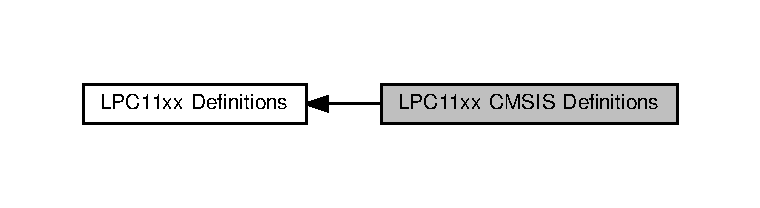
\includegraphics[width=350pt]{group___l_p_c11xx___c_m_s_i_s}
\end{center}
\end{figure}
\subsection*{Macros}
\begin{DoxyCompactItemize}
\item 
\#define \hyperlink{group___l_p_c11xx___c_m_s_i_s_ga4127d1b31aaf336fab3d7329d117f448}{\+\_\+\+\_\+\+M\+P\+U\+\_\+\+P\+R\+E\+S\+E\+NT}~0
\item 
\#define \hyperlink{group___l_p_c11xx___c_m_s_i_s_gae3fe3587d5100c787e02102ce3944460}{\+\_\+\+\_\+\+N\+V\+I\+C\+\_\+\+P\+R\+I\+O\+\_\+\+B\+I\+TS}~2
\item 
\#define \hyperlink{group___l_p_c11xx___c_m_s_i_s_gab58771b4ec03f9bdddc84770f7c95c68}{\+\_\+\+\_\+\+Vendor\+\_\+\+Sys\+Tick\+Config}~0
\end{DoxyCompactItemize}
\subsection*{Typedefs}
\begin{DoxyCompactItemize}
\item 
typedef enum \hyperlink{group___l_p_c11xx___c_m_s_i_s_ga666eb0caeb12ec0e281415592ae89083}{I\+R\+Qn} \hyperlink{group___l_p_c11xx___c_m_s_i_s_gac3af4a32370fb28c4ade8bf2add80251}{I\+R\+Qn\+\_\+\+Type}
\end{DoxyCompactItemize}
\subsection*{Enumerations}
\begin{DoxyCompactItemize}
\item 
enum \hyperlink{group___l_p_c11xx___c_m_s_i_s_ga666eb0caeb12ec0e281415592ae89083}{I\+R\+Qn} \{ \\*
\hyperlink{group___l_p_c11xx___c_m_s_i_s_gga666eb0caeb12ec0e281415592ae89083ade177d9c70c89e084093024b932a4e30}{Non\+Maskable\+Int\+\_\+\+I\+R\+Qn} = -\/14, 
\hyperlink{group___l_p_c11xx___c_m_s_i_s_gga666eb0caeb12ec0e281415592ae89083ab1a222a34a32f0ef5ac65e714efc1f85}{Hard\+Fault\+\_\+\+I\+R\+Qn} = -\/13, 
\hyperlink{group___l_p_c11xx___c_m_s_i_s_gga666eb0caeb12ec0e281415592ae89083a4ce820b3cc6cf3a796b41aadc0cf1237}{S\+V\+Call\+\_\+\+I\+R\+Qn} = -\/5, 
\hyperlink{group___l_p_c11xx___c_m_s_i_s_gga666eb0caeb12ec0e281415592ae89083a03c3cc89984928816d81793fc7bce4a2}{Pend\+S\+V\+\_\+\+I\+R\+Qn} = -\/2, 
\\*
\hyperlink{group___l_p_c11xx___c_m_s_i_s_gga666eb0caeb12ec0e281415592ae89083a6dbff8f8543325f3474cbae2446776e7}{Sys\+Tick\+\_\+\+I\+R\+Qn} = -\/1, 
\hyperlink{group___l_p_c11xx___c_m_s_i_s_gga666eb0caeb12ec0e281415592ae89083af01060170ceb0d6d577beacf41635ae0}{W\+A\+K\+E\+U\+P0\+\_\+\+I\+R\+Qn} = 0, 
\hyperlink{group___l_p_c11xx___c_m_s_i_s_gga666eb0caeb12ec0e281415592ae89083ad8e04985fa950d0759ce92d557a7ed7f}{W\+A\+K\+E\+U\+P1\+\_\+\+I\+R\+Qn} = 1, 
\hyperlink{group___l_p_c11xx___c_m_s_i_s_gga666eb0caeb12ec0e281415592ae89083ad4b2bb0ae5c1d52381f8cb9413affbf6}{W\+A\+K\+E\+U\+P2\+\_\+\+I\+R\+Qn} = 2, 
\\*
\hyperlink{group___l_p_c11xx___c_m_s_i_s_gga666eb0caeb12ec0e281415592ae89083a539f4e76913e12d41c7eec2e7c2239ed}{W\+A\+K\+E\+U\+P3\+\_\+\+I\+R\+Qn} = 3, 
\hyperlink{group___l_p_c11xx___c_m_s_i_s_gga666eb0caeb12ec0e281415592ae89083a3df13a5d451b495e0a86647b0750a837}{W\+A\+K\+E\+U\+P4\+\_\+\+I\+R\+Qn} = 4, 
\hyperlink{group___l_p_c11xx___c_m_s_i_s_gga666eb0caeb12ec0e281415592ae89083a3dfaf99bdb7c4b21bbc6a5e65d62ce5a}{W\+A\+K\+E\+U\+P5\+\_\+\+I\+R\+Qn} = 5, 
\hyperlink{group___l_p_c11xx___c_m_s_i_s_gga666eb0caeb12ec0e281415592ae89083ace715bb711cdb57694878d18789989a5}{W\+A\+K\+E\+U\+P6\+\_\+\+I\+R\+Qn} = 6, 
\\*
\hyperlink{group___l_p_c11xx___c_m_s_i_s_gga666eb0caeb12ec0e281415592ae89083a06b94ece7d467d84b4706956fbe9dc43}{W\+A\+K\+E\+U\+P7\+\_\+\+I\+R\+Qn} = 7, 
\hyperlink{group___l_p_c11xx___c_m_s_i_s_gga666eb0caeb12ec0e281415592ae89083ac84fd704de6c04930319dcc12c630698}{W\+A\+K\+E\+U\+P8\+\_\+\+I\+R\+Qn} = 8, 
\hyperlink{group___l_p_c11xx___c_m_s_i_s_gga666eb0caeb12ec0e281415592ae89083aa91c95e855a44d1d5c0b92ff2b979051}{W\+A\+K\+E\+U\+P9\+\_\+\+I\+R\+Qn} = 9, 
\hyperlink{group___l_p_c11xx___c_m_s_i_s_gga666eb0caeb12ec0e281415592ae89083a85209d0ff16184ac86dfdb01d8b26502}{W\+A\+K\+E\+U\+P10\+\_\+\+I\+R\+Qn} = 10, 
\\*
\hyperlink{group___l_p_c11xx___c_m_s_i_s_gga666eb0caeb12ec0e281415592ae89083a4f3db149d5fbb1513aa3c5e3fe9e7356}{W\+A\+K\+E\+U\+P11\+\_\+\+I\+R\+Qn} = 11, 
\hyperlink{group___l_p_c11xx___c_m_s_i_s_gga666eb0caeb12ec0e281415592ae89083a5595570597adb716c29763e5d5a2f484}{W\+A\+K\+E\+U\+P12\+\_\+\+I\+R\+Qn} = 12, 
\hyperlink{group___l_p_c11xx___c_m_s_i_s_gga666eb0caeb12ec0e281415592ae89083a20d0bdfa1654b723493895e3ea617cdb}{C\+A\+N\+\_\+\+I\+R\+Qn} = 13, 
\hyperlink{group___l_p_c11xx___c_m_s_i_s_gga666eb0caeb12ec0e281415592ae89083adcc0cfa46f0d13c2de0f3e826c10a789}{S\+S\+P1\+\_\+\+I\+R\+Qn} = 14, 
\\*
\hyperlink{group___l_p_c11xx___c_m_s_i_s_gga666eb0caeb12ec0e281415592ae89083adf8c31fe1c7ade2eb05f1414710dbce7}{I2\+C\+\_\+\+I\+R\+Qn} = 15, 
\hyperlink{group___l_p_c11xx___c_m_s_i_s_gga666eb0caeb12ec0e281415592ae89083a6f5ed57785374cb1ba3a1256e0d991be}{T\+I\+M\+E\+R\+\_\+16\+\_\+0\+\_\+\+I\+R\+Qn} = 16, 
\hyperlink{group___l_p_c11xx___c_m_s_i_s_gga666eb0caeb12ec0e281415592ae89083a9d13f0d0bbeb7bc1c75d512a94d66c9f}{T\+I\+M\+E\+R\+\_\+16\+\_\+1\+\_\+\+I\+R\+Qn} = 17, 
\hyperlink{group___l_p_c11xx___c_m_s_i_s_gga666eb0caeb12ec0e281415592ae89083a7e40673d4557974606b5d9670c0c50d0}{T\+I\+M\+E\+R\+\_\+32\+\_\+0\+\_\+\+I\+R\+Qn} = 18, 
\\*
\hyperlink{group___l_p_c11xx___c_m_s_i_s_gga666eb0caeb12ec0e281415592ae89083ac178a073454f598a32b7f95bcaba7679}{T\+I\+M\+E\+R\+\_\+32\+\_\+1\+\_\+\+I\+R\+Qn} = 19, 
\hyperlink{group___l_p_c11xx___c_m_s_i_s_gga666eb0caeb12ec0e281415592ae89083a6c8d6262fd7ecedc57b2fe9209be9765}{S\+S\+P0\+\_\+\+I\+R\+Qn} = 20, 
\hyperlink{group___l_p_c11xx___c_m_s_i_s_gga666eb0caeb12ec0e281415592ae89083a9d9be6e918c912367e393dae3480eabb}{U\+A\+R\+T\+\_\+\+I\+R\+Qn} = 21, 
\hyperlink{group___l_p_c11xx___c_m_s_i_s_gga666eb0caeb12ec0e281415592ae89083a2095f58b6c0de45b782b1196a0939e02}{Reserved0\+\_\+\+I\+R\+Qn} = 22, 
\\*
\hyperlink{group___l_p_c11xx___c_m_s_i_s_gga666eb0caeb12ec0e281415592ae89083add6253fd238cff7fa4b35e4ef81ffc07}{Reserved1\+\_\+\+I\+R\+Qn} = 23, 
\hyperlink{group___l_p_c11xx___c_m_s_i_s_gga666eb0caeb12ec0e281415592ae89083a4d69175258ae261dd545001e810421b3}{A\+D\+C\+\_\+\+I\+R\+Qn} = 24, 
\hyperlink{group___l_p_c11xx___c_m_s_i_s_gga666eb0caeb12ec0e281415592ae89083a78573b84a4133ef5812b33ce10dcba12}{W\+D\+T\+\_\+\+I\+R\+Qn} = 25, 
\hyperlink{group___l_p_c11xx___c_m_s_i_s_gga666eb0caeb12ec0e281415592ae89083ac2ee5960aed41ff349aa7a86c37e9ab2}{B\+O\+D\+\_\+\+I\+R\+Qn} = 26, 
\\*
\hyperlink{group___l_p_c11xx___c_m_s_i_s_gga666eb0caeb12ec0e281415592ae89083ab58dc79a081058857f73965f5305479b}{F\+M\+C\+\_\+\+I\+R\+Qn} = 27, 
\hyperlink{group___l_p_c11xx___c_m_s_i_s_gga666eb0caeb12ec0e281415592ae89083a14098dd2e0d0331c1e5f1f80dde14371}{E\+I\+N\+T3\+\_\+\+I\+R\+Qn} = 28, 
\hyperlink{group___l_p_c11xx___c_m_s_i_s_gga666eb0caeb12ec0e281415592ae89083a40ab356422a691418668d6bbfd9f17b9}{E\+I\+N\+T2\+\_\+\+I\+R\+Qn} = 29, 
\hyperlink{group___l_p_c11xx___c_m_s_i_s_gga666eb0caeb12ec0e281415592ae89083ad855ae101e21a04054a9844066900d7c}{E\+I\+N\+T1\+\_\+\+I\+R\+Qn} = 30, 
\\*
\hyperlink{group___l_p_c11xx___c_m_s_i_s_gga666eb0caeb12ec0e281415592ae89083a0a3db3233549f012f8ecb88f0510adcf}{E\+I\+N\+T0\+\_\+\+I\+R\+Qn} = 31
 \}
\end{DoxyCompactItemize}


\subsection{Detailed Description}
Configuration of the Cortex-\/\+M0 Processor and Core Peripherals 

\subsection{Macro Definition Documentation}
\index{L\+P\+C11xx C\+M\+S\+I\+S Definitions@{L\+P\+C11xx C\+M\+S\+I\+S Definitions}!\+\_\+\+\_\+\+M\+P\+U\+\_\+\+P\+R\+E\+S\+E\+NT@{\+\_\+\+\_\+\+M\+P\+U\+\_\+\+P\+R\+E\+S\+E\+NT}}
\index{\+\_\+\+\_\+\+M\+P\+U\+\_\+\+P\+R\+E\+S\+E\+NT@{\+\_\+\+\_\+\+M\+P\+U\+\_\+\+P\+R\+E\+S\+E\+NT}!L\+P\+C11xx C\+M\+S\+I\+S Definitions@{L\+P\+C11xx C\+M\+S\+I\+S Definitions}}
\subsubsection[{\texorpdfstring{\+\_\+\+\_\+\+M\+P\+U\+\_\+\+P\+R\+E\+S\+E\+NT}{__MPU_PRESENT}}]{\setlength{\rightskip}{0pt plus 5cm}\#define \+\_\+\+\_\+\+M\+P\+U\+\_\+\+P\+R\+E\+S\+E\+NT~0}\hypertarget{group___l_p_c11xx___c_m_s_i_s_ga4127d1b31aaf336fab3d7329d117f448}{}\label{group___l_p_c11xx___c_m_s_i_s_ga4127d1b31aaf336fab3d7329d117f448}
M\+PU present or not 

Definition at line 111 of file L\+P\+C11xx.\+h.

\index{L\+P\+C11xx C\+M\+S\+I\+S Definitions@{L\+P\+C11xx C\+M\+S\+I\+S Definitions}!\+\_\+\+\_\+\+N\+V\+I\+C\+\_\+\+P\+R\+I\+O\+\_\+\+B\+I\+TS@{\+\_\+\+\_\+\+N\+V\+I\+C\+\_\+\+P\+R\+I\+O\+\_\+\+B\+I\+TS}}
\index{\+\_\+\+\_\+\+N\+V\+I\+C\+\_\+\+P\+R\+I\+O\+\_\+\+B\+I\+TS@{\+\_\+\+\_\+\+N\+V\+I\+C\+\_\+\+P\+R\+I\+O\+\_\+\+B\+I\+TS}!L\+P\+C11xx C\+M\+S\+I\+S Definitions@{L\+P\+C11xx C\+M\+S\+I\+S Definitions}}
\subsubsection[{\texorpdfstring{\+\_\+\+\_\+\+N\+V\+I\+C\+\_\+\+P\+R\+I\+O\+\_\+\+B\+I\+TS}{__NVIC_PRIO_BITS}}]{\setlength{\rightskip}{0pt plus 5cm}\#define \+\_\+\+\_\+\+N\+V\+I\+C\+\_\+\+P\+R\+I\+O\+\_\+\+B\+I\+TS~2}\hypertarget{group___l_p_c11xx___c_m_s_i_s_gae3fe3587d5100c787e02102ce3944460}{}\label{group___l_p_c11xx___c_m_s_i_s_gae3fe3587d5100c787e02102ce3944460}
Number of Bits used for Priority Levels 

Definition at line 112 of file L\+P\+C11xx.\+h.

\index{L\+P\+C11xx C\+M\+S\+I\+S Definitions@{L\+P\+C11xx C\+M\+S\+I\+S Definitions}!\+\_\+\+\_\+\+Vendor\+\_\+\+Sys\+Tick\+Config@{\+\_\+\+\_\+\+Vendor\+\_\+\+Sys\+Tick\+Config}}
\index{\+\_\+\+\_\+\+Vendor\+\_\+\+Sys\+Tick\+Config@{\+\_\+\+\_\+\+Vendor\+\_\+\+Sys\+Tick\+Config}!L\+P\+C11xx C\+M\+S\+I\+S Definitions@{L\+P\+C11xx C\+M\+S\+I\+S Definitions}}
\subsubsection[{\texorpdfstring{\+\_\+\+\_\+\+Vendor\+\_\+\+Sys\+Tick\+Config}{__Vendor_SysTickConfig}}]{\setlength{\rightskip}{0pt plus 5cm}\#define \+\_\+\+\_\+\+Vendor\+\_\+\+Sys\+Tick\+Config~0}\hypertarget{group___l_p_c11xx___c_m_s_i_s_gab58771b4ec03f9bdddc84770f7c95c68}{}\label{group___l_p_c11xx___c_m_s_i_s_gab58771b4ec03f9bdddc84770f7c95c68}
Set to 1 if different Sys\+Tick Config is used 

Definition at line 113 of file L\+P\+C11xx.\+h.



\subsection{Typedef Documentation}
\index{L\+P\+C11xx C\+M\+S\+I\+S Definitions@{L\+P\+C11xx C\+M\+S\+I\+S Definitions}!I\+R\+Qn\+\_\+\+Type@{I\+R\+Qn\+\_\+\+Type}}
\index{I\+R\+Qn\+\_\+\+Type@{I\+R\+Qn\+\_\+\+Type}!L\+P\+C11xx C\+M\+S\+I\+S Definitions@{L\+P\+C11xx C\+M\+S\+I\+S Definitions}}
\subsubsection[{\texorpdfstring{I\+R\+Qn\+\_\+\+Type}{IRQn_Type}}]{\setlength{\rightskip}{0pt plus 5cm}typedef enum {\bf I\+R\+Qn}  {\bf I\+R\+Qn\+\_\+\+Type}}\hypertarget{group___l_p_c11xx___c_m_s_i_s_gac3af4a32370fb28c4ade8bf2add80251}{}\label{group___l_p_c11xx___c_m_s_i_s_gac3af4a32370fb28c4ade8bf2add80251}


\subsection{Enumeration Type Documentation}
\index{L\+P\+C11xx C\+M\+S\+I\+S Definitions@{L\+P\+C11xx C\+M\+S\+I\+S Definitions}!I\+R\+Qn@{I\+R\+Qn}}
\index{I\+R\+Qn@{I\+R\+Qn}!L\+P\+C11xx C\+M\+S\+I\+S Definitions@{L\+P\+C11xx C\+M\+S\+I\+S Definitions}}
\subsubsection[{\texorpdfstring{I\+R\+Qn}{IRQn}}]{\setlength{\rightskip}{0pt plus 5cm}enum {\bf I\+R\+Qn}}\hypertarget{group___l_p_c11xx___c_m_s_i_s_ga666eb0caeb12ec0e281415592ae89083}{}\label{group___l_p_c11xx___c_m_s_i_s_ga666eb0caeb12ec0e281415592ae89083}
\begin{Desc}
\item[Enumerator]\par
\begin{description}
\index{Non\+Maskable\+Int\+\_\+\+I\+R\+Qn@{Non\+Maskable\+Int\+\_\+\+I\+R\+Qn}!L\+P\+C11xx C\+M\+S\+I\+S Definitions@{L\+P\+C11xx C\+M\+S\+I\+S Definitions}}\index{L\+P\+C11xx C\+M\+S\+I\+S Definitions@{L\+P\+C11xx C\+M\+S\+I\+S Definitions}!Non\+Maskable\+Int\+\_\+\+I\+R\+Qn@{Non\+Maskable\+Int\+\_\+\+I\+R\+Qn}}\item[{\em 
Non\+Maskable\+Int\+\_\+\+I\+R\+Qn\hypertarget{group___l_p_c11xx___c_m_s_i_s_gga666eb0caeb12ec0e281415592ae89083ade177d9c70c89e084093024b932a4e30}{}\label{group___l_p_c11xx___c_m_s_i_s_gga666eb0caeb12ec0e281415592ae89083ade177d9c70c89e084093024b932a4e30}
}]2 Non Maskable Interrupt \index{Hard\+Fault\+\_\+\+I\+R\+Qn@{Hard\+Fault\+\_\+\+I\+R\+Qn}!L\+P\+C11xx C\+M\+S\+I\+S Definitions@{L\+P\+C11xx C\+M\+S\+I\+S Definitions}}\index{L\+P\+C11xx C\+M\+S\+I\+S Definitions@{L\+P\+C11xx C\+M\+S\+I\+S Definitions}!Hard\+Fault\+\_\+\+I\+R\+Qn@{Hard\+Fault\+\_\+\+I\+R\+Qn}}\item[{\em 
Hard\+Fault\+\_\+\+I\+R\+Qn\hypertarget{group___l_p_c11xx___c_m_s_i_s_gga666eb0caeb12ec0e281415592ae89083ab1a222a34a32f0ef5ac65e714efc1f85}{}\label{group___l_p_c11xx___c_m_s_i_s_gga666eb0caeb12ec0e281415592ae89083ab1a222a34a32f0ef5ac65e714efc1f85}
}]3 Cortex-\/\+M0 Hard Fault Interrupt \index{S\+V\+Call\+\_\+\+I\+R\+Qn@{S\+V\+Call\+\_\+\+I\+R\+Qn}!L\+P\+C11xx C\+M\+S\+I\+S Definitions@{L\+P\+C11xx C\+M\+S\+I\+S Definitions}}\index{L\+P\+C11xx C\+M\+S\+I\+S Definitions@{L\+P\+C11xx C\+M\+S\+I\+S Definitions}!S\+V\+Call\+\_\+\+I\+R\+Qn@{S\+V\+Call\+\_\+\+I\+R\+Qn}}\item[{\em 
S\+V\+Call\+\_\+\+I\+R\+Qn\hypertarget{group___l_p_c11xx___c_m_s_i_s_gga666eb0caeb12ec0e281415592ae89083a4ce820b3cc6cf3a796b41aadc0cf1237}{}\label{group___l_p_c11xx___c_m_s_i_s_gga666eb0caeb12ec0e281415592ae89083a4ce820b3cc6cf3a796b41aadc0cf1237}
}]11 Cortex-\/\+M0 SV Call Interrupt \index{Pend\+S\+V\+\_\+\+I\+R\+Qn@{Pend\+S\+V\+\_\+\+I\+R\+Qn}!L\+P\+C11xx C\+M\+S\+I\+S Definitions@{L\+P\+C11xx C\+M\+S\+I\+S Definitions}}\index{L\+P\+C11xx C\+M\+S\+I\+S Definitions@{L\+P\+C11xx C\+M\+S\+I\+S Definitions}!Pend\+S\+V\+\_\+\+I\+R\+Qn@{Pend\+S\+V\+\_\+\+I\+R\+Qn}}\item[{\em 
Pend\+S\+V\+\_\+\+I\+R\+Qn\hypertarget{group___l_p_c11xx___c_m_s_i_s_gga666eb0caeb12ec0e281415592ae89083a03c3cc89984928816d81793fc7bce4a2}{}\label{group___l_p_c11xx___c_m_s_i_s_gga666eb0caeb12ec0e281415592ae89083a03c3cc89984928816d81793fc7bce4a2}
}]14 Cortex-\/\+M0 Pend SV Interrupt \index{Sys\+Tick\+\_\+\+I\+R\+Qn@{Sys\+Tick\+\_\+\+I\+R\+Qn}!L\+P\+C11xx C\+M\+S\+I\+S Definitions@{L\+P\+C11xx C\+M\+S\+I\+S Definitions}}\index{L\+P\+C11xx C\+M\+S\+I\+S Definitions@{L\+P\+C11xx C\+M\+S\+I\+S Definitions}!Sys\+Tick\+\_\+\+I\+R\+Qn@{Sys\+Tick\+\_\+\+I\+R\+Qn}}\item[{\em 
Sys\+Tick\+\_\+\+I\+R\+Qn\hypertarget{group___l_p_c11xx___c_m_s_i_s_gga666eb0caeb12ec0e281415592ae89083a6dbff8f8543325f3474cbae2446776e7}{}\label{group___l_p_c11xx___c_m_s_i_s_gga666eb0caeb12ec0e281415592ae89083a6dbff8f8543325f3474cbae2446776e7}
}]15 Cortex-\/\+M0 System Tick Interrupt \index{W\+A\+K\+E\+U\+P0\+\_\+\+I\+R\+Qn@{W\+A\+K\+E\+U\+P0\+\_\+\+I\+R\+Qn}!L\+P\+C11xx C\+M\+S\+I\+S Definitions@{L\+P\+C11xx C\+M\+S\+I\+S Definitions}}\index{L\+P\+C11xx C\+M\+S\+I\+S Definitions@{L\+P\+C11xx C\+M\+S\+I\+S Definitions}!W\+A\+K\+E\+U\+P0\+\_\+\+I\+R\+Qn@{W\+A\+K\+E\+U\+P0\+\_\+\+I\+R\+Qn}}\item[{\em 
W\+A\+K\+E\+U\+P0\+\_\+\+I\+R\+Qn\hypertarget{group___l_p_c11xx___c_m_s_i_s_gga666eb0caeb12ec0e281415592ae89083af01060170ceb0d6d577beacf41635ae0}{}\label{group___l_p_c11xx___c_m_s_i_s_gga666eb0caeb12ec0e281415592ae89083af01060170ceb0d6d577beacf41635ae0}
}]All I/O pins can be used as wakeup source. \index{W\+A\+K\+E\+U\+P1\+\_\+\+I\+R\+Qn@{W\+A\+K\+E\+U\+P1\+\_\+\+I\+R\+Qn}!L\+P\+C11xx C\+M\+S\+I\+S Definitions@{L\+P\+C11xx C\+M\+S\+I\+S Definitions}}\index{L\+P\+C11xx C\+M\+S\+I\+S Definitions@{L\+P\+C11xx C\+M\+S\+I\+S Definitions}!W\+A\+K\+E\+U\+P1\+\_\+\+I\+R\+Qn@{W\+A\+K\+E\+U\+P1\+\_\+\+I\+R\+Qn}}\item[{\em 
W\+A\+K\+E\+U\+P1\+\_\+\+I\+R\+Qn\hypertarget{group___l_p_c11xx___c_m_s_i_s_gga666eb0caeb12ec0e281415592ae89083ad8e04985fa950d0759ce92d557a7ed7f}{}\label{group___l_p_c11xx___c_m_s_i_s_gga666eb0caeb12ec0e281415592ae89083ad8e04985fa950d0759ce92d557a7ed7f}
}]There are 13 pins in total for L\+P\+C11xx \index{W\+A\+K\+E\+U\+P2\+\_\+\+I\+R\+Qn@{W\+A\+K\+E\+U\+P2\+\_\+\+I\+R\+Qn}!L\+P\+C11xx C\+M\+S\+I\+S Definitions@{L\+P\+C11xx C\+M\+S\+I\+S Definitions}}\index{L\+P\+C11xx C\+M\+S\+I\+S Definitions@{L\+P\+C11xx C\+M\+S\+I\+S Definitions}!W\+A\+K\+E\+U\+P2\+\_\+\+I\+R\+Qn@{W\+A\+K\+E\+U\+P2\+\_\+\+I\+R\+Qn}}\item[{\em 
W\+A\+K\+E\+U\+P2\+\_\+\+I\+R\+Qn\hypertarget{group___l_p_c11xx___c_m_s_i_s_gga666eb0caeb12ec0e281415592ae89083ad4b2bb0ae5c1d52381f8cb9413affbf6}{}\label{group___l_p_c11xx___c_m_s_i_s_gga666eb0caeb12ec0e281415592ae89083ad4b2bb0ae5c1d52381f8cb9413affbf6}
}]\index{W\+A\+K\+E\+U\+P3\+\_\+\+I\+R\+Qn@{W\+A\+K\+E\+U\+P3\+\_\+\+I\+R\+Qn}!L\+P\+C11xx C\+M\+S\+I\+S Definitions@{L\+P\+C11xx C\+M\+S\+I\+S Definitions}}\index{L\+P\+C11xx C\+M\+S\+I\+S Definitions@{L\+P\+C11xx C\+M\+S\+I\+S Definitions}!W\+A\+K\+E\+U\+P3\+\_\+\+I\+R\+Qn@{W\+A\+K\+E\+U\+P3\+\_\+\+I\+R\+Qn}}\item[{\em 
W\+A\+K\+E\+U\+P3\+\_\+\+I\+R\+Qn\hypertarget{group___l_p_c11xx___c_m_s_i_s_gga666eb0caeb12ec0e281415592ae89083a539f4e76913e12d41c7eec2e7c2239ed}{}\label{group___l_p_c11xx___c_m_s_i_s_gga666eb0caeb12ec0e281415592ae89083a539f4e76913e12d41c7eec2e7c2239ed}
}]\index{W\+A\+K\+E\+U\+P4\+\_\+\+I\+R\+Qn@{W\+A\+K\+E\+U\+P4\+\_\+\+I\+R\+Qn}!L\+P\+C11xx C\+M\+S\+I\+S Definitions@{L\+P\+C11xx C\+M\+S\+I\+S Definitions}}\index{L\+P\+C11xx C\+M\+S\+I\+S Definitions@{L\+P\+C11xx C\+M\+S\+I\+S Definitions}!W\+A\+K\+E\+U\+P4\+\_\+\+I\+R\+Qn@{W\+A\+K\+E\+U\+P4\+\_\+\+I\+R\+Qn}}\item[{\em 
W\+A\+K\+E\+U\+P4\+\_\+\+I\+R\+Qn\hypertarget{group___l_p_c11xx___c_m_s_i_s_gga666eb0caeb12ec0e281415592ae89083a3df13a5d451b495e0a86647b0750a837}{}\label{group___l_p_c11xx___c_m_s_i_s_gga666eb0caeb12ec0e281415592ae89083a3df13a5d451b495e0a86647b0750a837}
}]\index{W\+A\+K\+E\+U\+P5\+\_\+\+I\+R\+Qn@{W\+A\+K\+E\+U\+P5\+\_\+\+I\+R\+Qn}!L\+P\+C11xx C\+M\+S\+I\+S Definitions@{L\+P\+C11xx C\+M\+S\+I\+S Definitions}}\index{L\+P\+C11xx C\+M\+S\+I\+S Definitions@{L\+P\+C11xx C\+M\+S\+I\+S Definitions}!W\+A\+K\+E\+U\+P5\+\_\+\+I\+R\+Qn@{W\+A\+K\+E\+U\+P5\+\_\+\+I\+R\+Qn}}\item[{\em 
W\+A\+K\+E\+U\+P5\+\_\+\+I\+R\+Qn\hypertarget{group___l_p_c11xx___c_m_s_i_s_gga666eb0caeb12ec0e281415592ae89083a3dfaf99bdb7c4b21bbc6a5e65d62ce5a}{}\label{group___l_p_c11xx___c_m_s_i_s_gga666eb0caeb12ec0e281415592ae89083a3dfaf99bdb7c4b21bbc6a5e65d62ce5a}
}]\index{W\+A\+K\+E\+U\+P6\+\_\+\+I\+R\+Qn@{W\+A\+K\+E\+U\+P6\+\_\+\+I\+R\+Qn}!L\+P\+C11xx C\+M\+S\+I\+S Definitions@{L\+P\+C11xx C\+M\+S\+I\+S Definitions}}\index{L\+P\+C11xx C\+M\+S\+I\+S Definitions@{L\+P\+C11xx C\+M\+S\+I\+S Definitions}!W\+A\+K\+E\+U\+P6\+\_\+\+I\+R\+Qn@{W\+A\+K\+E\+U\+P6\+\_\+\+I\+R\+Qn}}\item[{\em 
W\+A\+K\+E\+U\+P6\+\_\+\+I\+R\+Qn\hypertarget{group___l_p_c11xx___c_m_s_i_s_gga666eb0caeb12ec0e281415592ae89083ace715bb711cdb57694878d18789989a5}{}\label{group___l_p_c11xx___c_m_s_i_s_gga666eb0caeb12ec0e281415592ae89083ace715bb711cdb57694878d18789989a5}
}]\index{W\+A\+K\+E\+U\+P7\+\_\+\+I\+R\+Qn@{W\+A\+K\+E\+U\+P7\+\_\+\+I\+R\+Qn}!L\+P\+C11xx C\+M\+S\+I\+S Definitions@{L\+P\+C11xx C\+M\+S\+I\+S Definitions}}\index{L\+P\+C11xx C\+M\+S\+I\+S Definitions@{L\+P\+C11xx C\+M\+S\+I\+S Definitions}!W\+A\+K\+E\+U\+P7\+\_\+\+I\+R\+Qn@{W\+A\+K\+E\+U\+P7\+\_\+\+I\+R\+Qn}}\item[{\em 
W\+A\+K\+E\+U\+P7\+\_\+\+I\+R\+Qn\hypertarget{group___l_p_c11xx___c_m_s_i_s_gga666eb0caeb12ec0e281415592ae89083a06b94ece7d467d84b4706956fbe9dc43}{}\label{group___l_p_c11xx___c_m_s_i_s_gga666eb0caeb12ec0e281415592ae89083a06b94ece7d467d84b4706956fbe9dc43}
}]\index{W\+A\+K\+E\+U\+P8\+\_\+\+I\+R\+Qn@{W\+A\+K\+E\+U\+P8\+\_\+\+I\+R\+Qn}!L\+P\+C11xx C\+M\+S\+I\+S Definitions@{L\+P\+C11xx C\+M\+S\+I\+S Definitions}}\index{L\+P\+C11xx C\+M\+S\+I\+S Definitions@{L\+P\+C11xx C\+M\+S\+I\+S Definitions}!W\+A\+K\+E\+U\+P8\+\_\+\+I\+R\+Qn@{W\+A\+K\+E\+U\+P8\+\_\+\+I\+R\+Qn}}\item[{\em 
W\+A\+K\+E\+U\+P8\+\_\+\+I\+R\+Qn\hypertarget{group___l_p_c11xx___c_m_s_i_s_gga666eb0caeb12ec0e281415592ae89083ac84fd704de6c04930319dcc12c630698}{}\label{group___l_p_c11xx___c_m_s_i_s_gga666eb0caeb12ec0e281415592ae89083ac84fd704de6c04930319dcc12c630698}
}]\index{W\+A\+K\+E\+U\+P9\+\_\+\+I\+R\+Qn@{W\+A\+K\+E\+U\+P9\+\_\+\+I\+R\+Qn}!L\+P\+C11xx C\+M\+S\+I\+S Definitions@{L\+P\+C11xx C\+M\+S\+I\+S Definitions}}\index{L\+P\+C11xx C\+M\+S\+I\+S Definitions@{L\+P\+C11xx C\+M\+S\+I\+S Definitions}!W\+A\+K\+E\+U\+P9\+\_\+\+I\+R\+Qn@{W\+A\+K\+E\+U\+P9\+\_\+\+I\+R\+Qn}}\item[{\em 
W\+A\+K\+E\+U\+P9\+\_\+\+I\+R\+Qn\hypertarget{group___l_p_c11xx___c_m_s_i_s_gga666eb0caeb12ec0e281415592ae89083aa91c95e855a44d1d5c0b92ff2b979051}{}\label{group___l_p_c11xx___c_m_s_i_s_gga666eb0caeb12ec0e281415592ae89083aa91c95e855a44d1d5c0b92ff2b979051}
}]\index{W\+A\+K\+E\+U\+P10\+\_\+\+I\+R\+Qn@{W\+A\+K\+E\+U\+P10\+\_\+\+I\+R\+Qn}!L\+P\+C11xx C\+M\+S\+I\+S Definitions@{L\+P\+C11xx C\+M\+S\+I\+S Definitions}}\index{L\+P\+C11xx C\+M\+S\+I\+S Definitions@{L\+P\+C11xx C\+M\+S\+I\+S Definitions}!W\+A\+K\+E\+U\+P10\+\_\+\+I\+R\+Qn@{W\+A\+K\+E\+U\+P10\+\_\+\+I\+R\+Qn}}\item[{\em 
W\+A\+K\+E\+U\+P10\+\_\+\+I\+R\+Qn\hypertarget{group___l_p_c11xx___c_m_s_i_s_gga666eb0caeb12ec0e281415592ae89083a85209d0ff16184ac86dfdb01d8b26502}{}\label{group___l_p_c11xx___c_m_s_i_s_gga666eb0caeb12ec0e281415592ae89083a85209d0ff16184ac86dfdb01d8b26502}
}]\index{W\+A\+K\+E\+U\+P11\+\_\+\+I\+R\+Qn@{W\+A\+K\+E\+U\+P11\+\_\+\+I\+R\+Qn}!L\+P\+C11xx C\+M\+S\+I\+S Definitions@{L\+P\+C11xx C\+M\+S\+I\+S Definitions}}\index{L\+P\+C11xx C\+M\+S\+I\+S Definitions@{L\+P\+C11xx C\+M\+S\+I\+S Definitions}!W\+A\+K\+E\+U\+P11\+\_\+\+I\+R\+Qn@{W\+A\+K\+E\+U\+P11\+\_\+\+I\+R\+Qn}}\item[{\em 
W\+A\+K\+E\+U\+P11\+\_\+\+I\+R\+Qn\hypertarget{group___l_p_c11xx___c_m_s_i_s_gga666eb0caeb12ec0e281415592ae89083a4f3db149d5fbb1513aa3c5e3fe9e7356}{}\label{group___l_p_c11xx___c_m_s_i_s_gga666eb0caeb12ec0e281415592ae89083a4f3db149d5fbb1513aa3c5e3fe9e7356}
}]\index{W\+A\+K\+E\+U\+P12\+\_\+\+I\+R\+Qn@{W\+A\+K\+E\+U\+P12\+\_\+\+I\+R\+Qn}!L\+P\+C11xx C\+M\+S\+I\+S Definitions@{L\+P\+C11xx C\+M\+S\+I\+S Definitions}}\index{L\+P\+C11xx C\+M\+S\+I\+S Definitions@{L\+P\+C11xx C\+M\+S\+I\+S Definitions}!W\+A\+K\+E\+U\+P12\+\_\+\+I\+R\+Qn@{W\+A\+K\+E\+U\+P12\+\_\+\+I\+R\+Qn}}\item[{\em 
W\+A\+K\+E\+U\+P12\+\_\+\+I\+R\+Qn\hypertarget{group___l_p_c11xx___c_m_s_i_s_gga666eb0caeb12ec0e281415592ae89083a5595570597adb716c29763e5d5a2f484}{}\label{group___l_p_c11xx___c_m_s_i_s_gga666eb0caeb12ec0e281415592ae89083a5595570597adb716c29763e5d5a2f484}
}]\index{C\+A\+N\+\_\+\+I\+R\+Qn@{C\+A\+N\+\_\+\+I\+R\+Qn}!L\+P\+C11xx C\+M\+S\+I\+S Definitions@{L\+P\+C11xx C\+M\+S\+I\+S Definitions}}\index{L\+P\+C11xx C\+M\+S\+I\+S Definitions@{L\+P\+C11xx C\+M\+S\+I\+S Definitions}!C\+A\+N\+\_\+\+I\+R\+Qn@{C\+A\+N\+\_\+\+I\+R\+Qn}}\item[{\em 
C\+A\+N\+\_\+\+I\+R\+Qn\hypertarget{group___l_p_c11xx___c_m_s_i_s_gga666eb0caeb12ec0e281415592ae89083a20d0bdfa1654b723493895e3ea617cdb}{}\label{group___l_p_c11xx___c_m_s_i_s_gga666eb0caeb12ec0e281415592ae89083a20d0bdfa1654b723493895e3ea617cdb}
}]C\+AN Interrupt \index{S\+S\+P1\+\_\+\+I\+R\+Qn@{S\+S\+P1\+\_\+\+I\+R\+Qn}!L\+P\+C11xx C\+M\+S\+I\+S Definitions@{L\+P\+C11xx C\+M\+S\+I\+S Definitions}}\index{L\+P\+C11xx C\+M\+S\+I\+S Definitions@{L\+P\+C11xx C\+M\+S\+I\+S Definitions}!S\+S\+P1\+\_\+\+I\+R\+Qn@{S\+S\+P1\+\_\+\+I\+R\+Qn}}\item[{\em 
S\+S\+P1\+\_\+\+I\+R\+Qn\hypertarget{group___l_p_c11xx___c_m_s_i_s_gga666eb0caeb12ec0e281415592ae89083adcc0cfa46f0d13c2de0f3e826c10a789}{}\label{group___l_p_c11xx___c_m_s_i_s_gga666eb0caeb12ec0e281415592ae89083adcc0cfa46f0d13c2de0f3e826c10a789}
}]S\+S\+P1 Interrupt \index{I2\+C\+\_\+\+I\+R\+Qn@{I2\+C\+\_\+\+I\+R\+Qn}!L\+P\+C11xx C\+M\+S\+I\+S Definitions@{L\+P\+C11xx C\+M\+S\+I\+S Definitions}}\index{L\+P\+C11xx C\+M\+S\+I\+S Definitions@{L\+P\+C11xx C\+M\+S\+I\+S Definitions}!I2\+C\+\_\+\+I\+R\+Qn@{I2\+C\+\_\+\+I\+R\+Qn}}\item[{\em 
I2\+C\+\_\+\+I\+R\+Qn\hypertarget{group___l_p_c11xx___c_m_s_i_s_gga666eb0caeb12ec0e281415592ae89083adf8c31fe1c7ade2eb05f1414710dbce7}{}\label{group___l_p_c11xx___c_m_s_i_s_gga666eb0caeb12ec0e281415592ae89083adf8c31fe1c7ade2eb05f1414710dbce7}
}]I2C Interrupt \index{T\+I\+M\+E\+R\+\_\+16\+\_\+0\+\_\+\+I\+R\+Qn@{T\+I\+M\+E\+R\+\_\+16\+\_\+0\+\_\+\+I\+R\+Qn}!L\+P\+C11xx C\+M\+S\+I\+S Definitions@{L\+P\+C11xx C\+M\+S\+I\+S Definitions}}\index{L\+P\+C11xx C\+M\+S\+I\+S Definitions@{L\+P\+C11xx C\+M\+S\+I\+S Definitions}!T\+I\+M\+E\+R\+\_\+16\+\_\+0\+\_\+\+I\+R\+Qn@{T\+I\+M\+E\+R\+\_\+16\+\_\+0\+\_\+\+I\+R\+Qn}}\item[{\em 
T\+I\+M\+E\+R\+\_\+16\+\_\+0\+\_\+\+I\+R\+Qn\hypertarget{group___l_p_c11xx___c_m_s_i_s_gga666eb0caeb12ec0e281415592ae89083a6f5ed57785374cb1ba3a1256e0d991be}{}\label{group___l_p_c11xx___c_m_s_i_s_gga666eb0caeb12ec0e281415592ae89083a6f5ed57785374cb1ba3a1256e0d991be}
}]16-\/bit Timer0 Interrupt \index{T\+I\+M\+E\+R\+\_\+16\+\_\+1\+\_\+\+I\+R\+Qn@{T\+I\+M\+E\+R\+\_\+16\+\_\+1\+\_\+\+I\+R\+Qn}!L\+P\+C11xx C\+M\+S\+I\+S Definitions@{L\+P\+C11xx C\+M\+S\+I\+S Definitions}}\index{L\+P\+C11xx C\+M\+S\+I\+S Definitions@{L\+P\+C11xx C\+M\+S\+I\+S Definitions}!T\+I\+M\+E\+R\+\_\+16\+\_\+1\+\_\+\+I\+R\+Qn@{T\+I\+M\+E\+R\+\_\+16\+\_\+1\+\_\+\+I\+R\+Qn}}\item[{\em 
T\+I\+M\+E\+R\+\_\+16\+\_\+1\+\_\+\+I\+R\+Qn\hypertarget{group___l_p_c11xx___c_m_s_i_s_gga666eb0caeb12ec0e281415592ae89083a9d13f0d0bbeb7bc1c75d512a94d66c9f}{}\label{group___l_p_c11xx___c_m_s_i_s_gga666eb0caeb12ec0e281415592ae89083a9d13f0d0bbeb7bc1c75d512a94d66c9f}
}]16-\/bit Timer1 Interrupt \index{T\+I\+M\+E\+R\+\_\+32\+\_\+0\+\_\+\+I\+R\+Qn@{T\+I\+M\+E\+R\+\_\+32\+\_\+0\+\_\+\+I\+R\+Qn}!L\+P\+C11xx C\+M\+S\+I\+S Definitions@{L\+P\+C11xx C\+M\+S\+I\+S Definitions}}\index{L\+P\+C11xx C\+M\+S\+I\+S Definitions@{L\+P\+C11xx C\+M\+S\+I\+S Definitions}!T\+I\+M\+E\+R\+\_\+32\+\_\+0\+\_\+\+I\+R\+Qn@{T\+I\+M\+E\+R\+\_\+32\+\_\+0\+\_\+\+I\+R\+Qn}}\item[{\em 
T\+I\+M\+E\+R\+\_\+32\+\_\+0\+\_\+\+I\+R\+Qn\hypertarget{group___l_p_c11xx___c_m_s_i_s_gga666eb0caeb12ec0e281415592ae89083a7e40673d4557974606b5d9670c0c50d0}{}\label{group___l_p_c11xx___c_m_s_i_s_gga666eb0caeb12ec0e281415592ae89083a7e40673d4557974606b5d9670c0c50d0}
}]32-\/bit Timer0 Interrupt \index{T\+I\+M\+E\+R\+\_\+32\+\_\+1\+\_\+\+I\+R\+Qn@{T\+I\+M\+E\+R\+\_\+32\+\_\+1\+\_\+\+I\+R\+Qn}!L\+P\+C11xx C\+M\+S\+I\+S Definitions@{L\+P\+C11xx C\+M\+S\+I\+S Definitions}}\index{L\+P\+C11xx C\+M\+S\+I\+S Definitions@{L\+P\+C11xx C\+M\+S\+I\+S Definitions}!T\+I\+M\+E\+R\+\_\+32\+\_\+1\+\_\+\+I\+R\+Qn@{T\+I\+M\+E\+R\+\_\+32\+\_\+1\+\_\+\+I\+R\+Qn}}\item[{\em 
T\+I\+M\+E\+R\+\_\+32\+\_\+1\+\_\+\+I\+R\+Qn\hypertarget{group___l_p_c11xx___c_m_s_i_s_gga666eb0caeb12ec0e281415592ae89083ac178a073454f598a32b7f95bcaba7679}{}\label{group___l_p_c11xx___c_m_s_i_s_gga666eb0caeb12ec0e281415592ae89083ac178a073454f598a32b7f95bcaba7679}
}]32-\/bit Timer1 Interrupt \index{S\+S\+P0\+\_\+\+I\+R\+Qn@{S\+S\+P0\+\_\+\+I\+R\+Qn}!L\+P\+C11xx C\+M\+S\+I\+S Definitions@{L\+P\+C11xx C\+M\+S\+I\+S Definitions}}\index{L\+P\+C11xx C\+M\+S\+I\+S Definitions@{L\+P\+C11xx C\+M\+S\+I\+S Definitions}!S\+S\+P0\+\_\+\+I\+R\+Qn@{S\+S\+P0\+\_\+\+I\+R\+Qn}}\item[{\em 
S\+S\+P0\+\_\+\+I\+R\+Qn\hypertarget{group___l_p_c11xx___c_m_s_i_s_gga666eb0caeb12ec0e281415592ae89083a6c8d6262fd7ecedc57b2fe9209be9765}{}\label{group___l_p_c11xx___c_m_s_i_s_gga666eb0caeb12ec0e281415592ae89083a6c8d6262fd7ecedc57b2fe9209be9765}
}]S\+S\+P0 Interrupt \index{U\+A\+R\+T\+\_\+\+I\+R\+Qn@{U\+A\+R\+T\+\_\+\+I\+R\+Qn}!L\+P\+C11xx C\+M\+S\+I\+S Definitions@{L\+P\+C11xx C\+M\+S\+I\+S Definitions}}\index{L\+P\+C11xx C\+M\+S\+I\+S Definitions@{L\+P\+C11xx C\+M\+S\+I\+S Definitions}!U\+A\+R\+T\+\_\+\+I\+R\+Qn@{U\+A\+R\+T\+\_\+\+I\+R\+Qn}}\item[{\em 
U\+A\+R\+T\+\_\+\+I\+R\+Qn\hypertarget{group___l_p_c11xx___c_m_s_i_s_gga666eb0caeb12ec0e281415592ae89083a9d9be6e918c912367e393dae3480eabb}{}\label{group___l_p_c11xx___c_m_s_i_s_gga666eb0caeb12ec0e281415592ae89083a9d9be6e918c912367e393dae3480eabb}
}]U\+A\+RT Interrupt \index{Reserved0\+\_\+\+I\+R\+Qn@{Reserved0\+\_\+\+I\+R\+Qn}!L\+P\+C11xx C\+M\+S\+I\+S Definitions@{L\+P\+C11xx C\+M\+S\+I\+S Definitions}}\index{L\+P\+C11xx C\+M\+S\+I\+S Definitions@{L\+P\+C11xx C\+M\+S\+I\+S Definitions}!Reserved0\+\_\+\+I\+R\+Qn@{Reserved0\+\_\+\+I\+R\+Qn}}\item[{\em 
Reserved0\+\_\+\+I\+R\+Qn\hypertarget{group___l_p_c11xx___c_m_s_i_s_gga666eb0caeb12ec0e281415592ae89083a2095f58b6c0de45b782b1196a0939e02}{}\label{group___l_p_c11xx___c_m_s_i_s_gga666eb0caeb12ec0e281415592ae89083a2095f58b6c0de45b782b1196a0939e02}
}]Reserved Interrupt \index{Reserved1\+\_\+\+I\+R\+Qn@{Reserved1\+\_\+\+I\+R\+Qn}!L\+P\+C11xx C\+M\+S\+I\+S Definitions@{L\+P\+C11xx C\+M\+S\+I\+S Definitions}}\index{L\+P\+C11xx C\+M\+S\+I\+S Definitions@{L\+P\+C11xx C\+M\+S\+I\+S Definitions}!Reserved1\+\_\+\+I\+R\+Qn@{Reserved1\+\_\+\+I\+R\+Qn}}\item[{\em 
Reserved1\+\_\+\+I\+R\+Qn\hypertarget{group___l_p_c11xx___c_m_s_i_s_gga666eb0caeb12ec0e281415592ae89083add6253fd238cff7fa4b35e4ef81ffc07}{}\label{group___l_p_c11xx___c_m_s_i_s_gga666eb0caeb12ec0e281415592ae89083add6253fd238cff7fa4b35e4ef81ffc07}
}]\index{A\+D\+C\+\_\+\+I\+R\+Qn@{A\+D\+C\+\_\+\+I\+R\+Qn}!L\+P\+C11xx C\+M\+S\+I\+S Definitions@{L\+P\+C11xx C\+M\+S\+I\+S Definitions}}\index{L\+P\+C11xx C\+M\+S\+I\+S Definitions@{L\+P\+C11xx C\+M\+S\+I\+S Definitions}!A\+D\+C\+\_\+\+I\+R\+Qn@{A\+D\+C\+\_\+\+I\+R\+Qn}}\item[{\em 
A\+D\+C\+\_\+\+I\+R\+Qn\hypertarget{group___l_p_c11xx___c_m_s_i_s_gga666eb0caeb12ec0e281415592ae89083a4d69175258ae261dd545001e810421b3}{}\label{group___l_p_c11xx___c_m_s_i_s_gga666eb0caeb12ec0e281415592ae89083a4d69175258ae261dd545001e810421b3}
}]A/D Converter Interrupt \index{W\+D\+T\+\_\+\+I\+R\+Qn@{W\+D\+T\+\_\+\+I\+R\+Qn}!L\+P\+C11xx C\+M\+S\+I\+S Definitions@{L\+P\+C11xx C\+M\+S\+I\+S Definitions}}\index{L\+P\+C11xx C\+M\+S\+I\+S Definitions@{L\+P\+C11xx C\+M\+S\+I\+S Definitions}!W\+D\+T\+\_\+\+I\+R\+Qn@{W\+D\+T\+\_\+\+I\+R\+Qn}}\item[{\em 
W\+D\+T\+\_\+\+I\+R\+Qn\hypertarget{group___l_p_c11xx___c_m_s_i_s_gga666eb0caeb12ec0e281415592ae89083a78573b84a4133ef5812b33ce10dcba12}{}\label{group___l_p_c11xx___c_m_s_i_s_gga666eb0caeb12ec0e281415592ae89083a78573b84a4133ef5812b33ce10dcba12}
}]Watchdog timer Interrupt \index{B\+O\+D\+\_\+\+I\+R\+Qn@{B\+O\+D\+\_\+\+I\+R\+Qn}!L\+P\+C11xx C\+M\+S\+I\+S Definitions@{L\+P\+C11xx C\+M\+S\+I\+S Definitions}}\index{L\+P\+C11xx C\+M\+S\+I\+S Definitions@{L\+P\+C11xx C\+M\+S\+I\+S Definitions}!B\+O\+D\+\_\+\+I\+R\+Qn@{B\+O\+D\+\_\+\+I\+R\+Qn}}\item[{\em 
B\+O\+D\+\_\+\+I\+R\+Qn\hypertarget{group___l_p_c11xx___c_m_s_i_s_gga666eb0caeb12ec0e281415592ae89083ac2ee5960aed41ff349aa7a86c37e9ab2}{}\label{group___l_p_c11xx___c_m_s_i_s_gga666eb0caeb12ec0e281415592ae89083ac2ee5960aed41ff349aa7a86c37e9ab2}
}]Brown Out Detect(\+B\+O\+D) Interrupt \index{F\+M\+C\+\_\+\+I\+R\+Qn@{F\+M\+C\+\_\+\+I\+R\+Qn}!L\+P\+C11xx C\+M\+S\+I\+S Definitions@{L\+P\+C11xx C\+M\+S\+I\+S Definitions}}\index{L\+P\+C11xx C\+M\+S\+I\+S Definitions@{L\+P\+C11xx C\+M\+S\+I\+S Definitions}!F\+M\+C\+\_\+\+I\+R\+Qn@{F\+M\+C\+\_\+\+I\+R\+Qn}}\item[{\em 
F\+M\+C\+\_\+\+I\+R\+Qn\hypertarget{group___l_p_c11xx___c_m_s_i_s_gga666eb0caeb12ec0e281415592ae89083ab58dc79a081058857f73965f5305479b}{}\label{group___l_p_c11xx___c_m_s_i_s_gga666eb0caeb12ec0e281415592ae89083ab58dc79a081058857f73965f5305479b}
}]Flash Memory Controller Interrupt \index{E\+I\+N\+T3\+\_\+\+I\+R\+Qn@{E\+I\+N\+T3\+\_\+\+I\+R\+Qn}!L\+P\+C11xx C\+M\+S\+I\+S Definitions@{L\+P\+C11xx C\+M\+S\+I\+S Definitions}}\index{L\+P\+C11xx C\+M\+S\+I\+S Definitions@{L\+P\+C11xx C\+M\+S\+I\+S Definitions}!E\+I\+N\+T3\+\_\+\+I\+R\+Qn@{E\+I\+N\+T3\+\_\+\+I\+R\+Qn}}\item[{\em 
E\+I\+N\+T3\+\_\+\+I\+R\+Qn\hypertarget{group___l_p_c11xx___c_m_s_i_s_gga666eb0caeb12ec0e281415592ae89083a14098dd2e0d0331c1e5f1f80dde14371}{}\label{group___l_p_c11xx___c_m_s_i_s_gga666eb0caeb12ec0e281415592ae89083a14098dd2e0d0331c1e5f1f80dde14371}
}]External Interrupt 3 Interrupt \index{E\+I\+N\+T2\+\_\+\+I\+R\+Qn@{E\+I\+N\+T2\+\_\+\+I\+R\+Qn}!L\+P\+C11xx C\+M\+S\+I\+S Definitions@{L\+P\+C11xx C\+M\+S\+I\+S Definitions}}\index{L\+P\+C11xx C\+M\+S\+I\+S Definitions@{L\+P\+C11xx C\+M\+S\+I\+S Definitions}!E\+I\+N\+T2\+\_\+\+I\+R\+Qn@{E\+I\+N\+T2\+\_\+\+I\+R\+Qn}}\item[{\em 
E\+I\+N\+T2\+\_\+\+I\+R\+Qn\hypertarget{group___l_p_c11xx___c_m_s_i_s_gga666eb0caeb12ec0e281415592ae89083a40ab356422a691418668d6bbfd9f17b9}{}\label{group___l_p_c11xx___c_m_s_i_s_gga666eb0caeb12ec0e281415592ae89083a40ab356422a691418668d6bbfd9f17b9}
}]External Interrupt 2 Interrupt \index{E\+I\+N\+T1\+\_\+\+I\+R\+Qn@{E\+I\+N\+T1\+\_\+\+I\+R\+Qn}!L\+P\+C11xx C\+M\+S\+I\+S Definitions@{L\+P\+C11xx C\+M\+S\+I\+S Definitions}}\index{L\+P\+C11xx C\+M\+S\+I\+S Definitions@{L\+P\+C11xx C\+M\+S\+I\+S Definitions}!E\+I\+N\+T1\+\_\+\+I\+R\+Qn@{E\+I\+N\+T1\+\_\+\+I\+R\+Qn}}\item[{\em 
E\+I\+N\+T1\+\_\+\+I\+R\+Qn\hypertarget{group___l_p_c11xx___c_m_s_i_s_gga666eb0caeb12ec0e281415592ae89083ad855ae101e21a04054a9844066900d7c}{}\label{group___l_p_c11xx___c_m_s_i_s_gga666eb0caeb12ec0e281415592ae89083ad855ae101e21a04054a9844066900d7c}
}]External Interrupt 1 Interrupt \index{E\+I\+N\+T0\+\_\+\+I\+R\+Qn@{E\+I\+N\+T0\+\_\+\+I\+R\+Qn}!L\+P\+C11xx C\+M\+S\+I\+S Definitions@{L\+P\+C11xx C\+M\+S\+I\+S Definitions}}\index{L\+P\+C11xx C\+M\+S\+I\+S Definitions@{L\+P\+C11xx C\+M\+S\+I\+S Definitions}!E\+I\+N\+T0\+\_\+\+I\+R\+Qn@{E\+I\+N\+T0\+\_\+\+I\+R\+Qn}}\item[{\em 
E\+I\+N\+T0\+\_\+\+I\+R\+Qn\hypertarget{group___l_p_c11xx___c_m_s_i_s_gga666eb0caeb12ec0e281415592ae89083a0a3db3233549f012f8ecb88f0510adcf}{}\label{group___l_p_c11xx___c_m_s_i_s_gga666eb0caeb12ec0e281415592ae89083a0a3db3233549f012f8ecb88f0510adcf}
}]External Interrupt 0 Interrupt \end{description}
\end{Desc}


Definition at line 60 of file L\+P\+C11xx.\+h.


\hypertarget{group___l_p_c11xx___s_y_s_c_o_n}{}\section{L\+P\+C11xx System Control Block}
\label{group___l_p_c11xx___s_y_s_c_o_n}\index{L\+P\+C11xx System Control Block@{L\+P\+C11xx System Control Block}}
Collaboration diagram for L\+P\+C11xx System Control Block\+:\nopagebreak
\begin{figure}[H]
\begin{center}
\leavevmode
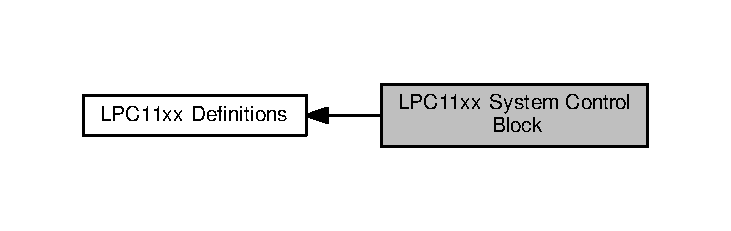
\includegraphics[width=350pt]{group___l_p_c11xx___s_y_s_c_o_n}
\end{center}
\end{figure}
\subsection*{Classes}
\begin{DoxyCompactItemize}
\item 
struct \hyperlink{struct_l_p_c___s_y_s_c_o_n___type_def}{L\+P\+C\+\_\+\+S\+Y\+S\+C\+O\+N\+\_\+\+Type\+Def}
\end{DoxyCompactItemize}


\subsection{Detailed Description}

\hypertarget{group___l_p_c11xx___i_o_c_o_n}{}\section{L\+P\+C11xx I/O Configuration Block}
\label{group___l_p_c11xx___i_o_c_o_n}\index{L\+P\+C11xx I/\+O Configuration Block@{L\+P\+C11xx I/\+O Configuration Block}}
Collaboration diagram for L\+P\+C11xx I/O Configuration Block\+:\nopagebreak
\begin{figure}[H]
\begin{center}
\leavevmode
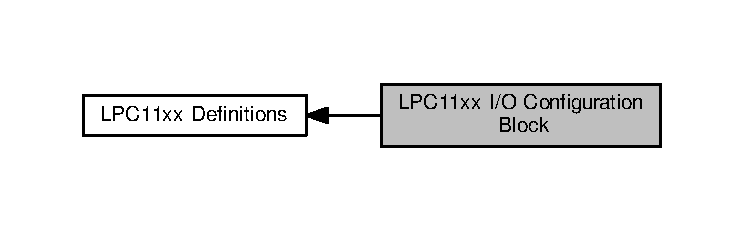
\includegraphics[width=350pt]{group___l_p_c11xx___i_o_c_o_n}
\end{center}
\end{figure}
\subsection*{Classes}
\begin{DoxyCompactItemize}
\item 
struct \hyperlink{struct_l_p_c___i_o_c_o_n___type_def}{L\+P\+C\+\_\+\+I\+O\+C\+O\+N\+\_\+\+Type\+Def}
\end{DoxyCompactItemize}


\subsection{Detailed Description}

\hypertarget{group___l_p_c11xx___p_m_u}{}\section{L\+P\+C11xx Power Management Unit}
\label{group___l_p_c11xx___p_m_u}\index{L\+P\+C11xx Power Management Unit@{L\+P\+C11xx Power Management Unit}}
Collaboration diagram for L\+P\+C11xx Power Management Unit\+:\nopagebreak
\begin{figure}[H]
\begin{center}
\leavevmode
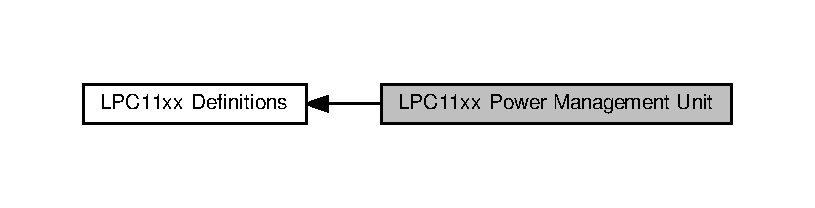
\includegraphics[width=350pt]{group___l_p_c11xx___p_m_u}
\end{center}
\end{figure}
\subsection*{Classes}
\begin{DoxyCompactItemize}
\item 
struct \hyperlink{struct_l_p_c___p_m_u___type_def}{L\+P\+C\+\_\+\+P\+M\+U\+\_\+\+Type\+Def}
\end{DoxyCompactItemize}


\subsection{Detailed Description}

\hypertarget{group___l_p_c11xx___g_p_i_o}{}\section{L\+P\+C11xx General Purpose Input/\+Output}
\label{group___l_p_c11xx___g_p_i_o}\index{L\+P\+C11xx General Purpose Input/\+Output@{L\+P\+C11xx General Purpose Input/\+Output}}
Collaboration diagram for L\+P\+C11xx General Purpose Input/\+Output\+:\nopagebreak
\begin{figure}[H]
\begin{center}
\leavevmode
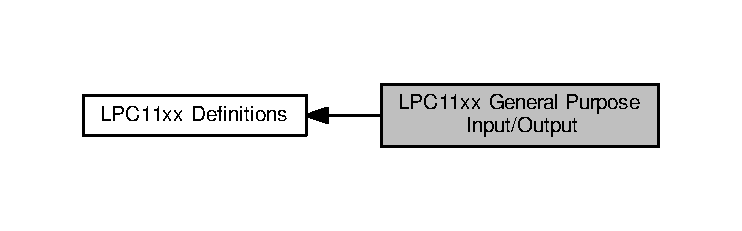
\includegraphics[width=350pt]{group___l_p_c11xx___g_p_i_o}
\end{center}
\end{figure}
\subsection*{Classes}
\begin{DoxyCompactItemize}
\item 
struct \hyperlink{struct_l_p_c___g_p_i_o___type_def}{L\+P\+C\+\_\+\+G\+P\+I\+O\+\_\+\+Type\+Def}
\end{DoxyCompactItemize}


\subsection{Detailed Description}

\hypertarget{group___l_p_c11xx___t_m_r}{}\section{L\+P\+C11xx 16/32-\/bit Counter/\+Timer}
\label{group___l_p_c11xx___t_m_r}\index{L\+P\+C11xx 16/32-\/bit Counter/\+Timer@{L\+P\+C11xx 16/32-\/bit Counter/\+Timer}}
Collaboration diagram for L\+P\+C11xx 16/32-\/bit Counter/\+Timer\+:\nopagebreak
\begin{figure}[H]
\begin{center}
\leavevmode
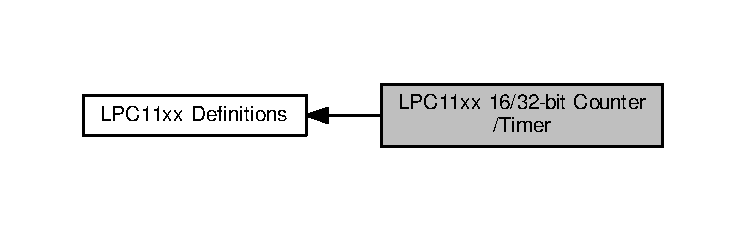
\includegraphics[width=350pt]{group___l_p_c11xx___t_m_r}
\end{center}
\end{figure}
\subsection*{Classes}
\begin{DoxyCompactItemize}
\item 
struct \hyperlink{struct_l_p_c___t_m_r___type_def}{L\+P\+C\+\_\+\+T\+M\+R\+\_\+\+Type\+Def}
\end{DoxyCompactItemize}


\subsection{Detailed Description}

\hypertarget{group___l_p_c11xx___u_a_r_t}{}\section{L\+P\+C11xx Universal Asynchronous Receiver/\+Transmitter}
\label{group___l_p_c11xx___u_a_r_t}\index{L\+P\+C11xx Universal Asynchronous Receiver/\+Transmitter@{L\+P\+C11xx Universal Asynchronous Receiver/\+Transmitter}}
Collaboration diagram for L\+P\+C11xx Universal Asynchronous Receiver/\+Transmitter\+:\nopagebreak
\begin{figure}[H]
\begin{center}
\leavevmode
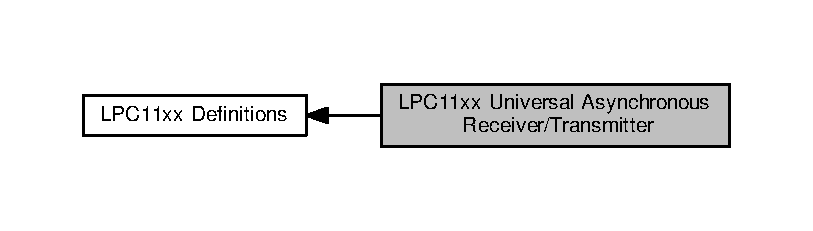
\includegraphics[width=350pt]{group___l_p_c11xx___u_a_r_t}
\end{center}
\end{figure}
\subsection*{Classes}
\begin{DoxyCompactItemize}
\item 
struct \hyperlink{struct_l_p_c___u_a_r_t___type_def}{L\+P\+C\+\_\+\+U\+A\+R\+T\+\_\+\+Type\+Def}
\end{DoxyCompactItemize}


\subsection{Detailed Description}

\hypertarget{group___l_p_c11xx___s_s_p}{}\section{L\+P\+C11xx Synchronous Serial Port}
\label{group___l_p_c11xx___s_s_p}\index{L\+P\+C11xx Synchronous Serial Port@{L\+P\+C11xx Synchronous Serial Port}}
Collaboration diagram for L\+P\+C11xx Synchronous Serial Port\+:\nopagebreak
\begin{figure}[H]
\begin{center}
\leavevmode
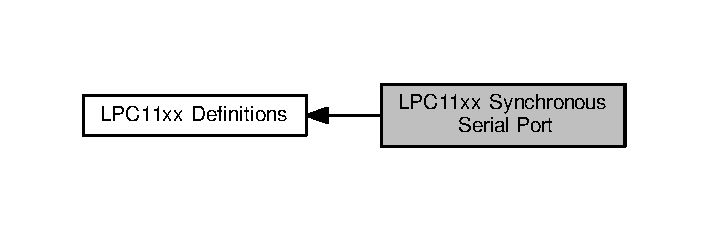
\includegraphics[width=340pt]{group___l_p_c11xx___s_s_p}
\end{center}
\end{figure}
\subsection*{Classes}
\begin{DoxyCompactItemize}
\item 
struct \hyperlink{struct_l_p_c___s_s_p___type_def}{L\+P\+C\+\_\+\+S\+S\+P\+\_\+\+Type\+Def}
\end{DoxyCompactItemize}


\subsection{Detailed Description}

\hypertarget{group___l_p_c11xx___i2_c}{}\section{L\+P\+C11xx I2\+C-\/\+Bus Interface}
\label{group___l_p_c11xx___i2_c}\index{L\+P\+C11xx I2\+C-\/\+Bus Interface@{L\+P\+C11xx I2\+C-\/\+Bus Interface}}
Collaboration diagram for L\+P\+C11xx I2\+C-\/\+Bus Interface\+:\nopagebreak
\begin{figure}[H]
\begin{center}
\leavevmode
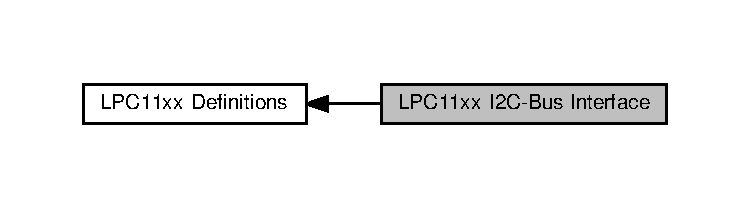
\includegraphics[width=350pt]{group___l_p_c11xx___i2_c}
\end{center}
\end{figure}
\subsection*{Classes}
\begin{DoxyCompactItemize}
\item 
struct \hyperlink{struct_l_p_c___i2_c___type_def}{L\+P\+C\+\_\+\+I2\+C\+\_\+\+Type\+Def}
\end{DoxyCompactItemize}


\subsection{Detailed Description}

\hypertarget{group___l_p_c11xx___w_d_t}{}\section{L\+P\+C11xx Watch\+Dog Timer}
\label{group___l_p_c11xx___w_d_t}\index{L\+P\+C11xx Watch\+Dog Timer@{L\+P\+C11xx Watch\+Dog Timer}}
Collaboration diagram for L\+P\+C11xx Watch\+Dog Timer\+:\nopagebreak
\begin{figure}[H]
\begin{center}
\leavevmode
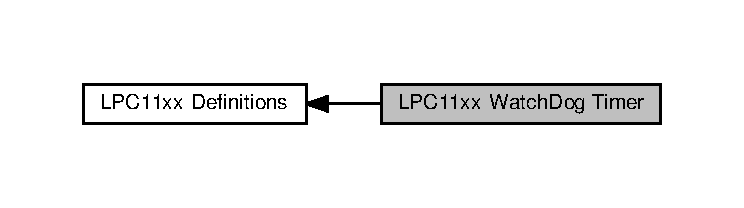
\includegraphics[width=350pt]{group___l_p_c11xx___w_d_t}
\end{center}
\end{figure}
\subsection*{Classes}
\begin{DoxyCompactItemize}
\item 
struct \hyperlink{struct_l_p_c___w_d_t___type_def}{L\+P\+C\+\_\+\+W\+D\+T\+\_\+\+Type\+Def}
\end{DoxyCompactItemize}


\subsection{Detailed Description}

\hypertarget{group___l_p_c11xx___a_d_c}{}\section{L\+P\+C11xx Analog-\/to-\/\+Digital Converter}
\label{group___l_p_c11xx___a_d_c}\index{L\+P\+C11xx Analog-\/to-\/\+Digital Converter@{L\+P\+C11xx Analog-\/to-\/\+Digital Converter}}
Collaboration diagram for L\+P\+C11xx Analog-\/to-\/\+Digital Converter\+:\nopagebreak
\begin{figure}[H]
\begin{center}
\leavevmode
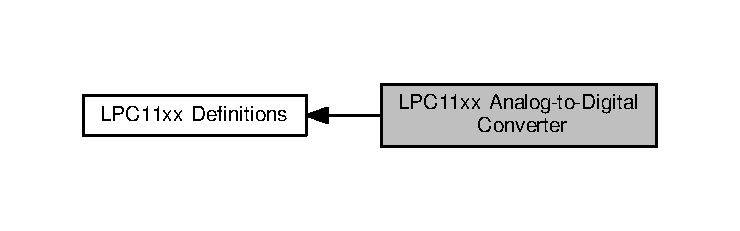
\includegraphics[width=350pt]{group___l_p_c11xx___a_d_c}
\end{center}
\end{figure}
\subsection*{Classes}
\begin{DoxyCompactItemize}
\item 
struct \hyperlink{struct_l_p_c___a_d_c___type_def}{L\+P\+C\+\_\+\+A\+D\+C\+\_\+\+Type\+Def}
\end{DoxyCompactItemize}


\subsection{Detailed Description}

\hypertarget{group___l_p_c11xx___c_a_n}{}\section{L\+P\+C11xx Controller Area Network(C\+AN)}
\label{group___l_p_c11xx___c_a_n}\index{L\+P\+C11xx Controller Area Network(\+C\+A\+N)@{L\+P\+C11xx Controller Area Network(\+C\+A\+N)}}
Collaboration diagram for L\+P\+C11xx Controller Area Network(C\+AN)\+:\nopagebreak
\begin{figure}[H]
\begin{center}
\leavevmode
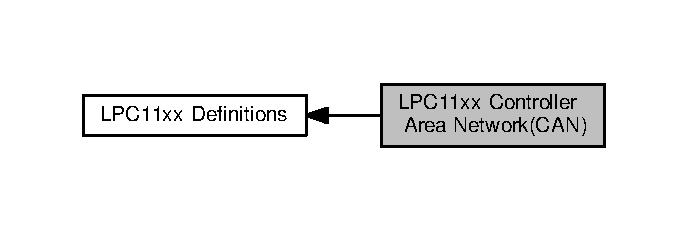
\includegraphics[width=330pt]{group___l_p_c11xx___c_a_n}
\end{center}
\end{figure}
\subsection*{Classes}
\begin{DoxyCompactItemize}
\item 
struct \hyperlink{struct_l_p_c___c_a_n___type_def}{L\+P\+C\+\_\+\+C\+A\+N\+\_\+\+Type\+Def}
\end{DoxyCompactItemize}


\subsection{Detailed Description}

\chapter{Class Documentation}
\hypertarget{union_a_p_s_r___type}{}\section{A\+P\+S\+R\+\_\+\+Type Union Reference}
\label{union_a_p_s_r___type}\index{A\+P\+S\+R\+\_\+\+Type@{A\+P\+S\+R\+\_\+\+Type}}


Union type to access the Application Program Status Register (A\+P\+SR).  




{\ttfamily \#include $<$core\+\_\+cm0.\+h$>$}

\subsection*{Public Attributes}
\begin{DoxyCompactItemize}
\item 
\begin{tabbing}
xx\=xx\=xx\=xx\=xx\=xx\=xx\=xx\=xx\=\kill
struct \{\\
\>uint32\_t \hyperlink{union_a_p_s_r___type_afbce95646fd514c10aa85ec0a33db728}{\_reserved0}:27\\
\>uint32\_t \hyperlink{union_a_p_s_r___type_a22d10913489d24ab08bd83457daa88de}{Q}:1\\
\>uint32\_t \hyperlink{union_a_p_s_r___type_a8004d224aacb78ca37774c35f9156e7e}{V}:1\\
\>uint32\_t \hyperlink{union_a_p_s_r___type_a86e2c5b891ecef1ab55b1edac0da79a6}{C}:1\\
\>uint32\_t \hyperlink{union_a_p_s_r___type_a3b04d58738b66a28ff13f23d8b0ba7e5}{Z}:1\\
\>uint32\_t \hyperlink{union_a_p_s_r___type_a7e7bbba9b00b0bb3283dc07f1abe37e0}{N}:1\\
\} \hyperlink{union_a_p_s_r___type_a7dbc79a057ded4b11ca5323fc2d5ab14}{b}\\

\end{tabbing}\item 
uint32\+\_\+t \hyperlink{union_a_p_s_r___type_ae4c2ef8c9430d7b7bef5cbfbbaed3a94}{w}
\end{DoxyCompactItemize}


\subsection{Detailed Description}
Union type to access the Application Program Status Register (A\+P\+SR). 

Definition at line 149 of file core\+\_\+cm0.\+h.



\subsection{Member Data Documentation}
\index{A\+P\+S\+R\+\_\+\+Type@{A\+P\+S\+R\+\_\+\+Type}!\+\_\+reserved0@{\+\_\+reserved0}}
\index{\+\_\+reserved0@{\+\_\+reserved0}!A\+P\+S\+R\+\_\+\+Type@{A\+P\+S\+R\+\_\+\+Type}}
\subsubsection[{\texorpdfstring{\+\_\+reserved0}{_reserved0}}]{\setlength{\rightskip}{0pt plus 5cm}uint32\+\_\+t A\+P\+S\+R\+\_\+\+Type\+::\+\_\+reserved0}\hypertarget{union_a_p_s_r___type_afbce95646fd514c10aa85ec0a33db728}{}\label{union_a_p_s_r___type_afbce95646fd514c10aa85ec0a33db728}
bit\+: 0..26 Reserved 

Definition at line 154 of file core\+\_\+cm0.\+h.

\index{A\+P\+S\+R\+\_\+\+Type@{A\+P\+S\+R\+\_\+\+Type}!b@{b}}
\index{b@{b}!A\+P\+S\+R\+\_\+\+Type@{A\+P\+S\+R\+\_\+\+Type}}
\subsubsection[{\texorpdfstring{b}{b}}]{\setlength{\rightskip}{0pt plus 5cm}struct \{ ... \}   A\+P\+S\+R\+\_\+\+Type\+::b}\hypertarget{union_a_p_s_r___type_a7dbc79a057ded4b11ca5323fc2d5ab14}{}\label{union_a_p_s_r___type_a7dbc79a057ded4b11ca5323fc2d5ab14}
Structure used for bit access \index{A\+P\+S\+R\+\_\+\+Type@{A\+P\+S\+R\+\_\+\+Type}!C@{C}}
\index{C@{C}!A\+P\+S\+R\+\_\+\+Type@{A\+P\+S\+R\+\_\+\+Type}}
\subsubsection[{\texorpdfstring{C}{C}}]{\setlength{\rightskip}{0pt plus 5cm}uint32\+\_\+t A\+P\+S\+R\+\_\+\+Type\+::C}\hypertarget{union_a_p_s_r___type_a86e2c5b891ecef1ab55b1edac0da79a6}{}\label{union_a_p_s_r___type_a86e2c5b891ecef1ab55b1edac0da79a6}
bit\+: 29 Carry condition code flag 

Definition at line 162 of file core\+\_\+cm0.\+h.

\index{A\+P\+S\+R\+\_\+\+Type@{A\+P\+S\+R\+\_\+\+Type}!N@{N}}
\index{N@{N}!A\+P\+S\+R\+\_\+\+Type@{A\+P\+S\+R\+\_\+\+Type}}
\subsubsection[{\texorpdfstring{N}{N}}]{\setlength{\rightskip}{0pt plus 5cm}uint32\+\_\+t A\+P\+S\+R\+\_\+\+Type\+::N}\hypertarget{union_a_p_s_r___type_a7e7bbba9b00b0bb3283dc07f1abe37e0}{}\label{union_a_p_s_r___type_a7e7bbba9b00b0bb3283dc07f1abe37e0}
bit\+: 31 Negative condition code flag 

Definition at line 164 of file core\+\_\+cm0.\+h.

\index{A\+P\+S\+R\+\_\+\+Type@{A\+P\+S\+R\+\_\+\+Type}!Q@{Q}}
\index{Q@{Q}!A\+P\+S\+R\+\_\+\+Type@{A\+P\+S\+R\+\_\+\+Type}}
\subsubsection[{\texorpdfstring{Q}{Q}}]{\setlength{\rightskip}{0pt plus 5cm}uint32\+\_\+t A\+P\+S\+R\+\_\+\+Type\+::Q}\hypertarget{union_a_p_s_r___type_a22d10913489d24ab08bd83457daa88de}{}\label{union_a_p_s_r___type_a22d10913489d24ab08bd83457daa88de}
bit\+: 27 Saturation condition flag 

Definition at line 160 of file core\+\_\+cm0.\+h.

\index{A\+P\+S\+R\+\_\+\+Type@{A\+P\+S\+R\+\_\+\+Type}!V@{V}}
\index{V@{V}!A\+P\+S\+R\+\_\+\+Type@{A\+P\+S\+R\+\_\+\+Type}}
\subsubsection[{\texorpdfstring{V}{V}}]{\setlength{\rightskip}{0pt plus 5cm}uint32\+\_\+t A\+P\+S\+R\+\_\+\+Type\+::V}\hypertarget{union_a_p_s_r___type_a8004d224aacb78ca37774c35f9156e7e}{}\label{union_a_p_s_r___type_a8004d224aacb78ca37774c35f9156e7e}
bit\+: 28 Overflow condition code flag 

Definition at line 161 of file core\+\_\+cm0.\+h.

\index{A\+P\+S\+R\+\_\+\+Type@{A\+P\+S\+R\+\_\+\+Type}!w@{w}}
\index{w@{w}!A\+P\+S\+R\+\_\+\+Type@{A\+P\+S\+R\+\_\+\+Type}}
\subsubsection[{\texorpdfstring{w}{w}}]{\setlength{\rightskip}{0pt plus 5cm}uint32\+\_\+t A\+P\+S\+R\+\_\+\+Type\+::w}\hypertarget{union_a_p_s_r___type_ae4c2ef8c9430d7b7bef5cbfbbaed3a94}{}\label{union_a_p_s_r___type_ae4c2ef8c9430d7b7bef5cbfbbaed3a94}
Type used for word access 

Definition at line 166 of file core\+\_\+cm0.\+h.

\index{A\+P\+S\+R\+\_\+\+Type@{A\+P\+S\+R\+\_\+\+Type}!Z@{Z}}
\index{Z@{Z}!A\+P\+S\+R\+\_\+\+Type@{A\+P\+S\+R\+\_\+\+Type}}
\subsubsection[{\texorpdfstring{Z}{Z}}]{\setlength{\rightskip}{0pt plus 5cm}uint32\+\_\+t A\+P\+S\+R\+\_\+\+Type\+::Z}\hypertarget{union_a_p_s_r___type_a3b04d58738b66a28ff13f23d8b0ba7e5}{}\label{union_a_p_s_r___type_a3b04d58738b66a28ff13f23d8b0ba7e5}
bit\+: 30 Zero condition code flag 

Definition at line 163 of file core\+\_\+cm0.\+h.



The documentation for this union was generated from the following file\+:\begin{DoxyCompactItemize}
\item 
/home/piro8/\+Documentos/\+T\+I\+N\+O\+C2/\+T\+I\+N\+O\+C2\+\_\+\+F\+I\+R\+M\+W\+A\+R\+E\+\_\+\+F\+R\+E\+E\+R\+T\+O\+S/\+C\+M\+S\+I\+Sv2p00\+\_\+\+L\+P\+C1102/inc/\hyperlink{core__cm0_8h}{core\+\_\+cm0.\+h}\end{DoxyCompactItemize}

\hypertarget{union_c_o_n_t_r_o_l___type}{}\section{C\+O\+N\+T\+R\+O\+L\+\_\+\+Type Union Reference}
\label{union_c_o_n_t_r_o_l___type}\index{C\+O\+N\+T\+R\+O\+L\+\_\+\+Type@{C\+O\+N\+T\+R\+O\+L\+\_\+\+Type}}


Union type to access the Control Registers (C\+O\+N\+T\+R\+OL).  




{\ttfamily \#include $<$core\+\_\+cm0.\+h$>$}

\subsection*{Public Attributes}
\begin{DoxyCompactItemize}
\item 
\begin{tabbing}
xx\=xx\=xx\=xx\=xx\=xx\=xx\=xx\=xx\=\kill
struct \{\\
\>uint32\_t \hyperlink{union_c_o_n_t_r_o_l___type_a35c1732cf153b7b5c4bd321cf1de9605}{nPRIV}:1\\
\>uint32\_t \hyperlink{union_c_o_n_t_r_o_l___type_a8cc085fea1c50a8bd9adea63931ee8e2}{SPSEL}:1\\
\>uint32\_t \hyperlink{union_c_o_n_t_r_o_l___type_ac62cfff08e6f055e0101785bad7094cd}{FPCA}:1\\
\>uint32\_t \hyperlink{union_c_o_n_t_r_o_l___type_af8c314273a1e4970a5671bd7f8184f50}{\_reserved0}:29\\
\} \hyperlink{union_c_o_n_t_r_o_l___type_adc6a38ab2980d0e9577b5a871da14eb9}{b}\\

\end{tabbing}\item 
uint32\+\_\+t \hyperlink{union_c_o_n_t_r_o_l___type_a6b642cca3d96da660b1198c133ca2a1f}{w}
\end{DoxyCompactItemize}


\subsection{Detailed Description}
Union type to access the Control Registers (C\+O\+N\+T\+R\+OL). 

Definition at line 211 of file core\+\_\+cm0.\+h.



\subsection{Member Data Documentation}
\index{C\+O\+N\+T\+R\+O\+L\+\_\+\+Type@{C\+O\+N\+T\+R\+O\+L\+\_\+\+Type}!\+\_\+reserved0@{\+\_\+reserved0}}
\index{\+\_\+reserved0@{\+\_\+reserved0}!C\+O\+N\+T\+R\+O\+L\+\_\+\+Type@{C\+O\+N\+T\+R\+O\+L\+\_\+\+Type}}
\subsubsection[{\texorpdfstring{\+\_\+reserved0}{_reserved0}}]{\setlength{\rightskip}{0pt plus 5cm}uint32\+\_\+t C\+O\+N\+T\+R\+O\+L\+\_\+\+Type\+::\+\_\+reserved0}\hypertarget{union_c_o_n_t_r_o_l___type_af8c314273a1e4970a5671bd7f8184f50}{}\label{union_c_o_n_t_r_o_l___type_af8c314273a1e4970a5671bd7f8184f50}
bit\+: 3..31 Reserved 

Definition at line 218 of file core\+\_\+cm0.\+h.

\index{C\+O\+N\+T\+R\+O\+L\+\_\+\+Type@{C\+O\+N\+T\+R\+O\+L\+\_\+\+Type}!b@{b}}
\index{b@{b}!C\+O\+N\+T\+R\+O\+L\+\_\+\+Type@{C\+O\+N\+T\+R\+O\+L\+\_\+\+Type}}
\subsubsection[{\texorpdfstring{b}{b}}]{\setlength{\rightskip}{0pt plus 5cm}struct \{ ... \}   C\+O\+N\+T\+R\+O\+L\+\_\+\+Type\+::b}\hypertarget{union_c_o_n_t_r_o_l___type_adc6a38ab2980d0e9577b5a871da14eb9}{}\label{union_c_o_n_t_r_o_l___type_adc6a38ab2980d0e9577b5a871da14eb9}
Structure used for bit access \index{C\+O\+N\+T\+R\+O\+L\+\_\+\+Type@{C\+O\+N\+T\+R\+O\+L\+\_\+\+Type}!F\+P\+CA@{F\+P\+CA}}
\index{F\+P\+CA@{F\+P\+CA}!C\+O\+N\+T\+R\+O\+L\+\_\+\+Type@{C\+O\+N\+T\+R\+O\+L\+\_\+\+Type}}
\subsubsection[{\texorpdfstring{F\+P\+CA}{FPCA}}]{\setlength{\rightskip}{0pt plus 5cm}uint32\+\_\+t C\+O\+N\+T\+R\+O\+L\+\_\+\+Type\+::\+F\+P\+CA}\hypertarget{union_c_o_n_t_r_o_l___type_ac62cfff08e6f055e0101785bad7094cd}{}\label{union_c_o_n_t_r_o_l___type_ac62cfff08e6f055e0101785bad7094cd}
bit\+: 2 FP extension active flag 

Definition at line 217 of file core\+\_\+cm0.\+h.

\index{C\+O\+N\+T\+R\+O\+L\+\_\+\+Type@{C\+O\+N\+T\+R\+O\+L\+\_\+\+Type}!n\+P\+R\+IV@{n\+P\+R\+IV}}
\index{n\+P\+R\+IV@{n\+P\+R\+IV}!C\+O\+N\+T\+R\+O\+L\+\_\+\+Type@{C\+O\+N\+T\+R\+O\+L\+\_\+\+Type}}
\subsubsection[{\texorpdfstring{n\+P\+R\+IV}{nPRIV}}]{\setlength{\rightskip}{0pt plus 5cm}uint32\+\_\+t C\+O\+N\+T\+R\+O\+L\+\_\+\+Type\+::n\+P\+R\+IV}\hypertarget{union_c_o_n_t_r_o_l___type_a35c1732cf153b7b5c4bd321cf1de9605}{}\label{union_c_o_n_t_r_o_l___type_a35c1732cf153b7b5c4bd321cf1de9605}
bit\+: 0 Execution privilege in Thread mode 

Definition at line 215 of file core\+\_\+cm0.\+h.

\index{C\+O\+N\+T\+R\+O\+L\+\_\+\+Type@{C\+O\+N\+T\+R\+O\+L\+\_\+\+Type}!S\+P\+S\+EL@{S\+P\+S\+EL}}
\index{S\+P\+S\+EL@{S\+P\+S\+EL}!C\+O\+N\+T\+R\+O\+L\+\_\+\+Type@{C\+O\+N\+T\+R\+O\+L\+\_\+\+Type}}
\subsubsection[{\texorpdfstring{S\+P\+S\+EL}{SPSEL}}]{\setlength{\rightskip}{0pt plus 5cm}uint32\+\_\+t C\+O\+N\+T\+R\+O\+L\+\_\+\+Type\+::\+S\+P\+S\+EL}\hypertarget{union_c_o_n_t_r_o_l___type_a8cc085fea1c50a8bd9adea63931ee8e2}{}\label{union_c_o_n_t_r_o_l___type_a8cc085fea1c50a8bd9adea63931ee8e2}
bit\+: 1 Stack to be used 

Definition at line 216 of file core\+\_\+cm0.\+h.

\index{C\+O\+N\+T\+R\+O\+L\+\_\+\+Type@{C\+O\+N\+T\+R\+O\+L\+\_\+\+Type}!w@{w}}
\index{w@{w}!C\+O\+N\+T\+R\+O\+L\+\_\+\+Type@{C\+O\+N\+T\+R\+O\+L\+\_\+\+Type}}
\subsubsection[{\texorpdfstring{w}{w}}]{\setlength{\rightskip}{0pt plus 5cm}uint32\+\_\+t C\+O\+N\+T\+R\+O\+L\+\_\+\+Type\+::w}\hypertarget{union_c_o_n_t_r_o_l___type_a6b642cca3d96da660b1198c133ca2a1f}{}\label{union_c_o_n_t_r_o_l___type_a6b642cca3d96da660b1198c133ca2a1f}
Type used for word access 

Definition at line 220 of file core\+\_\+cm0.\+h.



The documentation for this union was generated from the following file\+:\begin{DoxyCompactItemize}
\item 
/home/piro8/\+Documentos/\+T\+I\+N\+O\+C2/\+T\+I\+N\+O\+C2\+\_\+\+F\+I\+R\+M\+W\+A\+R\+E\+\_\+\+F\+R\+E\+E\+R\+T\+O\+S/\+C\+M\+S\+I\+Sv2p00\+\_\+\+L\+P\+C1102/inc/\hyperlink{core__cm0_8h}{core\+\_\+cm0.\+h}\end{DoxyCompactItemize}

\hypertarget{union_i_p_s_r___type}{}\section{I\+P\+S\+R\+\_\+\+Type Union Reference}
\label{union_i_p_s_r___type}\index{I\+P\+S\+R\+\_\+\+Type@{I\+P\+S\+R\+\_\+\+Type}}


Union type to access the Interrupt Program Status Register (I\+P\+SR).  




{\ttfamily \#include $<$core\+\_\+cm0.\+h$>$}

\subsection*{Public Attributes}
\begin{DoxyCompactItemize}
\item 
\begin{tabbing}
xx\=xx\=xx\=xx\=xx\=xx\=xx\=xx\=xx\=\kill
struct \{\\
\>uint32\_t \hyperlink{union_i_p_s_r___type_ab46e5f1b2f4d17cfb9aca4fffcbb2fa5}{ISR}:9\\
\>uint32\_t \hyperlink{union_i_p_s_r___type_ad2eb0a06de4f03f58874a727716aa9aa}{\_reserved0}:23\\
\} \hyperlink{union_i_p_s_r___type_add0d6497bd50c25569ea22b48a03ec50}{b}\\

\end{tabbing}\item 
uint32\+\_\+t \hyperlink{union_i_p_s_r___type_a4adca999d3a0bc1ae682d73ea7cfa879}{w}
\end{DoxyCompactItemize}


\subsection{Detailed Description}
Union type to access the Interrupt Program Status Register (I\+P\+SR). 

Definition at line 172 of file core\+\_\+cm0.\+h.



\subsection{Member Data Documentation}
\index{I\+P\+S\+R\+\_\+\+Type@{I\+P\+S\+R\+\_\+\+Type}!\+\_\+reserved0@{\+\_\+reserved0}}
\index{\+\_\+reserved0@{\+\_\+reserved0}!I\+P\+S\+R\+\_\+\+Type@{I\+P\+S\+R\+\_\+\+Type}}
\subsubsection[{\texorpdfstring{\+\_\+reserved0}{_reserved0}}]{\setlength{\rightskip}{0pt plus 5cm}uint32\+\_\+t I\+P\+S\+R\+\_\+\+Type\+::\+\_\+reserved0}\hypertarget{union_i_p_s_r___type_ad2eb0a06de4f03f58874a727716aa9aa}{}\label{union_i_p_s_r___type_ad2eb0a06de4f03f58874a727716aa9aa}
bit\+: 9..31 Reserved 

Definition at line 177 of file core\+\_\+cm0.\+h.

\index{I\+P\+S\+R\+\_\+\+Type@{I\+P\+S\+R\+\_\+\+Type}!b@{b}}
\index{b@{b}!I\+P\+S\+R\+\_\+\+Type@{I\+P\+S\+R\+\_\+\+Type}}
\subsubsection[{\texorpdfstring{b}{b}}]{\setlength{\rightskip}{0pt plus 5cm}struct \{ ... \}   I\+P\+S\+R\+\_\+\+Type\+::b}\hypertarget{union_i_p_s_r___type_add0d6497bd50c25569ea22b48a03ec50}{}\label{union_i_p_s_r___type_add0d6497bd50c25569ea22b48a03ec50}
Structure used for bit access \index{I\+P\+S\+R\+\_\+\+Type@{I\+P\+S\+R\+\_\+\+Type}!I\+SR@{I\+SR}}
\index{I\+SR@{I\+SR}!I\+P\+S\+R\+\_\+\+Type@{I\+P\+S\+R\+\_\+\+Type}}
\subsubsection[{\texorpdfstring{I\+SR}{ISR}}]{\setlength{\rightskip}{0pt plus 5cm}uint32\+\_\+t I\+P\+S\+R\+\_\+\+Type\+::\+I\+SR}\hypertarget{union_i_p_s_r___type_ab46e5f1b2f4d17cfb9aca4fffcbb2fa5}{}\label{union_i_p_s_r___type_ab46e5f1b2f4d17cfb9aca4fffcbb2fa5}
bit\+: 0.. 8 Exception number 

Definition at line 176 of file core\+\_\+cm0.\+h.

\index{I\+P\+S\+R\+\_\+\+Type@{I\+P\+S\+R\+\_\+\+Type}!w@{w}}
\index{w@{w}!I\+P\+S\+R\+\_\+\+Type@{I\+P\+S\+R\+\_\+\+Type}}
\subsubsection[{\texorpdfstring{w}{w}}]{\setlength{\rightskip}{0pt plus 5cm}uint32\+\_\+t I\+P\+S\+R\+\_\+\+Type\+::w}\hypertarget{union_i_p_s_r___type_a4adca999d3a0bc1ae682d73ea7cfa879}{}\label{union_i_p_s_r___type_a4adca999d3a0bc1ae682d73ea7cfa879}
Type used for word access 

Definition at line 179 of file core\+\_\+cm0.\+h.



The documentation for this union was generated from the following file\+:\begin{DoxyCompactItemize}
\item 
/home/piro8/\+Documentos/\+T\+I\+N\+O\+C2/\+T\+I\+N\+O\+C2\+\_\+\+F\+I\+R\+M\+W\+A\+R\+E\+\_\+\+F\+R\+E\+E\+R\+T\+O\+S/\+C\+M\+S\+I\+Sv2p00\+\_\+\+L\+P\+C1102/inc/\hyperlink{core__cm0_8h}{core\+\_\+cm0.\+h}\end{DoxyCompactItemize}

\hypertarget{struct_l_p_c___a_d_c___type_def}{}\section{L\+P\+C\+\_\+\+A\+D\+C\+\_\+\+Type\+Def Struct Reference}
\label{struct_l_p_c___a_d_c___type_def}\index{L\+P\+C\+\_\+\+A\+D\+C\+\_\+\+Type\+Def@{L\+P\+C\+\_\+\+A\+D\+C\+\_\+\+Type\+Def}}


{\ttfamily \#include $<$L\+P\+C11xx.\+h$>$}

\subsection*{Public Attributes}
\begin{DoxyCompactItemize}
\item 
\hyperlink{group___c_m_s_i_s__core__definitions_gaec43007d9998a0a0e01faede4133d6be}{\+\_\+\+\_\+\+IO} uint32\+\_\+t \hyperlink{group___l_p_c11xx___definitions_ga5d9525fbad55b4d561ec1f4c8e1a6c75}{CR}
\item 
\hyperlink{group___c_m_s_i_s__core__definitions_gaec43007d9998a0a0e01faede4133d6be}{\+\_\+\+\_\+\+IO} uint32\+\_\+t \hyperlink{group___l_p_c11xx___definitions_ga6891936fcf717753e53ffed97d6329dd}{G\+DR}
\item 
uint32\+\_\+t \hyperlink{group___l_p_c11xx___definitions_ga40cf73fb4dbf0486e17c338b59481012}{R\+E\+S\+E\+R\+V\+E\+D0}
\item 
\hyperlink{group___c_m_s_i_s__core__definitions_gaec43007d9998a0a0e01faede4133d6be}{\+\_\+\+\_\+\+IO} uint32\+\_\+t \hyperlink{group___l_p_c11xx___definitions_gafd88fd018d5d8464442e7c6bbabda5a2}{I\+N\+T\+EN}
\item 
\hyperlink{group___c_m_s_i_s__core__definitions_gaec43007d9998a0a0e01faede4133d6be}{\+\_\+\+\_\+\+IO} uint32\+\_\+t \hyperlink{group___l_p_c11xx___definitions_gacb2fe5ff342d70582f0f476c880ab2cc}{DR} \mbox{[}8\mbox{]}
\item 
\hyperlink{group___c_m_s_i_s__core__definitions_gaf63697ed9952cc71e1225efe205f6cd3}{\+\_\+\+\_\+I} uint32\+\_\+t \hyperlink{group___l_p_c11xx___definitions_ga1bdbd1fea2c9424fa59b47192fcf63d0}{S\+T\+AT}
\end{DoxyCompactItemize}


\subsection{Detailed Description}


Definition at line 467 of file L\+P\+C11xx.\+h.



The documentation for this struct was generated from the following file\+:\begin{DoxyCompactItemize}
\item 
/home/piro8/\+Documentos/\+T\+I\+N\+O\+C2/\+T\+I\+N\+O\+C2\+\_\+\+F\+I\+R\+M\+W\+A\+R\+E\+\_\+\+F\+R\+E\+E\+R\+T\+O\+S/\+C\+M\+S\+I\+Sv2p00\+\_\+\+L\+P\+C1102/inc/\hyperlink{_l_p_c11xx_8h}{L\+P\+C11xx.\+h}\end{DoxyCompactItemize}

\hypertarget{struct_l_p_c___c_a_n___type_def}{}\section{L\+P\+C\+\_\+\+C\+A\+N\+\_\+\+Type\+Def Struct Reference}
\label{struct_l_p_c___c_a_n___type_def}\index{L\+P\+C\+\_\+\+C\+A\+N\+\_\+\+Type\+Def@{L\+P\+C\+\_\+\+C\+A\+N\+\_\+\+Type\+Def}}


{\ttfamily \#include $<$L\+P\+C11xx.\+h$>$}

\subsection*{Public Attributes}
\begin{DoxyCompactItemize}
\item 
\hyperlink{group___c_m_s_i_s__core__definitions_gaec43007d9998a0a0e01faede4133d6be}{\+\_\+\+\_\+\+IO} uint32\+\_\+t \hyperlink{group___l_p_c11xx___definitions_ga8add56ab65690f15125719eb9eda4470}{C\+N\+TL}
\item 
\hyperlink{group___c_m_s_i_s__core__definitions_gaec43007d9998a0a0e01faede4133d6be}{\+\_\+\+\_\+\+IO} uint32\+\_\+t \hyperlink{group___l_p_c11xx___definitions_ga0b209f4b82c9f56bbd7b3bbd74ea0c71}{S\+T\+AT}
\item 
\hyperlink{group___c_m_s_i_s__core__definitions_gaec43007d9998a0a0e01faede4133d6be}{\+\_\+\+\_\+\+IO} uint32\+\_\+t \hyperlink{group___l_p_c11xx___definitions_ga2c69811a8a235e77f2066a96610b9f96}{EC}
\item 
\hyperlink{group___c_m_s_i_s__core__definitions_gaec43007d9998a0a0e01faede4133d6be}{\+\_\+\+\_\+\+IO} uint32\+\_\+t \hyperlink{group___l_p_c11xx___definitions_ga5c23c4ebe014434dacbc966d68846f21}{BT}
\item 
\hyperlink{group___c_m_s_i_s__core__definitions_gaec43007d9998a0a0e01faede4133d6be}{\+\_\+\+\_\+\+IO} uint32\+\_\+t \hyperlink{group___l_p_c11xx___definitions_ga3019df722c0ccf0e0f0a3480c985d188}{I\+NT}
\item 
\hyperlink{group___c_m_s_i_s__core__definitions_gaec43007d9998a0a0e01faede4133d6be}{\+\_\+\+\_\+\+IO} uint32\+\_\+t \hyperlink{group___l_p_c11xx___definitions_gac41d8021c6279949be65ac66cb5d35d2}{T\+E\+ST}
\item 
\hyperlink{group___c_m_s_i_s__core__definitions_gaec43007d9998a0a0e01faede4133d6be}{\+\_\+\+\_\+\+IO} uint32\+\_\+t \hyperlink{group___l_p_c11xx___definitions_ga3b7c082aa752b35a5167f664ba74aafc}{B\+R\+PE}
\item 
uint32\+\_\+t \hyperlink{group___l_p_c11xx___definitions_ga97aaf019e54287718e9867461d05fccb}{R\+E\+S\+E\+R\+V\+E\+D0}
\item 
\hyperlink{group___c_m_s_i_s__core__definitions_gaec43007d9998a0a0e01faede4133d6be}{\+\_\+\+\_\+\+IO} uint32\+\_\+t \hyperlink{group___l_p_c11xx___definitions_ga45151797d18dbb4cdee027788d7dc2f6}{I\+F1\+\_\+\+C\+M\+D\+R\+EQ}
\item 
\hyperlink{group___c_m_s_i_s__core__definitions_gaec43007d9998a0a0e01faede4133d6be}{\+\_\+\+\_\+\+IO} uint32\+\_\+t \hyperlink{group___l_p_c11xx___definitions_ga3b6c7f057c23660d4f7e07737ac841cf}{I\+F1\+\_\+\+C\+M\+D\+M\+SK}
\item 
\hyperlink{group___c_m_s_i_s__core__definitions_gaec43007d9998a0a0e01faede4133d6be}{\+\_\+\+\_\+\+IO} uint32\+\_\+t \hyperlink{group___l_p_c11xx___definitions_gaae755f1728176c2ac1afcc2f40b1e12f}{I\+F1\+\_\+\+M\+S\+K1}
\item 
\hyperlink{group___c_m_s_i_s__core__definitions_gaec43007d9998a0a0e01faede4133d6be}{\+\_\+\+\_\+\+IO} uint32\+\_\+t \hyperlink{group___l_p_c11xx___definitions_ga455246305e2379030ba4d9bcdc28d219}{I\+F1\+\_\+\+M\+S\+K2}
\item 
\hyperlink{group___c_m_s_i_s__core__definitions_gaec43007d9998a0a0e01faede4133d6be}{\+\_\+\+\_\+\+IO} uint32\+\_\+t \hyperlink{group___l_p_c11xx___definitions_ga8bfa0cbf26f7c7b19964205260840c16}{I\+F1\+\_\+\+A\+R\+B1}
\item 
\hyperlink{group___c_m_s_i_s__core__definitions_gaec43007d9998a0a0e01faede4133d6be}{\+\_\+\+\_\+\+IO} uint32\+\_\+t \hyperlink{group___l_p_c11xx___definitions_gafb8cc57b47b3f40fb755b775734ae96c}{I\+F1\+\_\+\+A\+R\+B2}
\item 
\hyperlink{group___c_m_s_i_s__core__definitions_gaec43007d9998a0a0e01faede4133d6be}{\+\_\+\+\_\+\+IO} uint32\+\_\+t \hyperlink{group___l_p_c11xx___definitions_ga6b153c866a4e4b8bbadae2f8f3ac4855}{I\+F1\+\_\+\+M\+C\+T\+RL}
\item 
\hyperlink{group___c_m_s_i_s__core__definitions_gaec43007d9998a0a0e01faede4133d6be}{\+\_\+\+\_\+\+IO} uint32\+\_\+t \hyperlink{group___l_p_c11xx___definitions_ga7c33859386353ab630c9103410551b08}{I\+F1\+\_\+\+D\+A1}
\item 
\hyperlink{group___c_m_s_i_s__core__definitions_gaec43007d9998a0a0e01faede4133d6be}{\+\_\+\+\_\+\+IO} uint32\+\_\+t \hyperlink{group___l_p_c11xx___definitions_gadd4a84037c610c93a86d6584efb55d66}{I\+F1\+\_\+\+D\+A2}
\item 
\hyperlink{group___c_m_s_i_s__core__definitions_gaec43007d9998a0a0e01faede4133d6be}{\+\_\+\+\_\+\+IO} uint32\+\_\+t \hyperlink{group___l_p_c11xx___definitions_ga79bfadf7004722f5a0776f5229e341ce}{I\+F1\+\_\+\+D\+B1}
\item 
\hyperlink{group___c_m_s_i_s__core__definitions_gaec43007d9998a0a0e01faede4133d6be}{\+\_\+\+\_\+\+IO} uint32\+\_\+t \hyperlink{group___l_p_c11xx___definitions_gae2190ebf4f611a5a19c554610949e637}{I\+F1\+\_\+\+D\+B2}
\item 
uint32\+\_\+t \hyperlink{group___l_p_c11xx___definitions_ga67db9e4622642f886f81d4225bfd6ca3}{R\+E\+S\+E\+R\+V\+E\+D1} \mbox{[}13\mbox{]}
\item 
\hyperlink{group___c_m_s_i_s__core__definitions_gaec43007d9998a0a0e01faede4133d6be}{\+\_\+\+\_\+\+IO} uint32\+\_\+t \hyperlink{group___l_p_c11xx___definitions_ga23eb87edb95f06094e7fdc2b00542fdb}{I\+F2\+\_\+\+C\+M\+D\+R\+EQ}
\item 
\hyperlink{group___c_m_s_i_s__core__definitions_gaec43007d9998a0a0e01faede4133d6be}{\+\_\+\+\_\+\+IO} uint32\+\_\+t \hyperlink{group___l_p_c11xx___definitions_gac1841a007c665765fd5bc9ec2c3bd9bb}{I\+F2\+\_\+\+C\+M\+D\+M\+SK}
\item 
\hyperlink{group___c_m_s_i_s__core__definitions_gaec43007d9998a0a0e01faede4133d6be}{\+\_\+\+\_\+\+IO} uint32\+\_\+t \hyperlink{group___l_p_c11xx___definitions_ga4e085765bc1424bcda239e5c98c9f183}{I\+F2\+\_\+\+M\+S\+K1}
\item 
\hyperlink{group___c_m_s_i_s__core__definitions_gaec43007d9998a0a0e01faede4133d6be}{\+\_\+\+\_\+\+IO} uint32\+\_\+t \hyperlink{group___l_p_c11xx___definitions_gae8c1675d6e43b7ddf76fdcadb83e3d7b}{I\+F2\+\_\+\+M\+S\+K2}
\item 
\hyperlink{group___c_m_s_i_s__core__definitions_gaec43007d9998a0a0e01faede4133d6be}{\+\_\+\+\_\+\+IO} uint32\+\_\+t \hyperlink{group___l_p_c11xx___definitions_ga00e0f296ba765d6587677a2fecdd3692}{I\+F2\+\_\+\+A\+R\+B1}
\item 
\hyperlink{group___c_m_s_i_s__core__definitions_gaec43007d9998a0a0e01faede4133d6be}{\+\_\+\+\_\+\+IO} uint32\+\_\+t \hyperlink{group___l_p_c11xx___definitions_ga0d05f7ebf62d51c6ab973c78e04cfa4f}{I\+F2\+\_\+\+A\+R\+B2}
\item 
\hyperlink{group___c_m_s_i_s__core__definitions_gaec43007d9998a0a0e01faede4133d6be}{\+\_\+\+\_\+\+IO} uint32\+\_\+t \hyperlink{group___l_p_c11xx___definitions_ga0aefb018eeb2b0ee1f41e09f41fee754}{I\+F2\+\_\+\+M\+C\+T\+RL}
\item 
\hyperlink{group___c_m_s_i_s__core__definitions_gaec43007d9998a0a0e01faede4133d6be}{\+\_\+\+\_\+\+IO} uint32\+\_\+t \hyperlink{group___l_p_c11xx___definitions_gafb6089f5fac0b908d26b073c05ae099e}{I\+F2\+\_\+\+D\+A1}
\item 
\hyperlink{group___c_m_s_i_s__core__definitions_gaec43007d9998a0a0e01faede4133d6be}{\+\_\+\+\_\+\+IO} uint32\+\_\+t \hyperlink{group___l_p_c11xx___definitions_ga148142dc7364af3052e4d6f9eb40994c}{I\+F2\+\_\+\+D\+A2}
\item 
\hyperlink{group___c_m_s_i_s__core__definitions_gaec43007d9998a0a0e01faede4133d6be}{\+\_\+\+\_\+\+IO} uint32\+\_\+t \hyperlink{group___l_p_c11xx___definitions_gac012bbcf7bb1c4652d6bafed70b18597}{I\+F2\+\_\+\+D\+B1}
\item 
\hyperlink{group___c_m_s_i_s__core__definitions_gaec43007d9998a0a0e01faede4133d6be}{\+\_\+\+\_\+\+IO} uint32\+\_\+t \hyperlink{group___l_p_c11xx___definitions_gaf9b91f8118a022094558ac2d0b7ece77}{I\+F2\+\_\+\+D\+B2}
\item 
uint32\+\_\+t \hyperlink{group___l_p_c11xx___definitions_gaccfdfc30dad1c391034d049062b2821b}{R\+E\+S\+E\+R\+V\+E\+D2} \mbox{[}21\mbox{]}
\item 
\hyperlink{group___c_m_s_i_s__core__definitions_gaf63697ed9952cc71e1225efe205f6cd3}{\+\_\+\+\_\+I} uint32\+\_\+t \hyperlink{group___l_p_c11xx___definitions_ga4d4eebce6a7b6b29f8556faec742ab9a}{T\+X\+R\+E\+Q1}
\item 
\hyperlink{group___c_m_s_i_s__core__definitions_gaf63697ed9952cc71e1225efe205f6cd3}{\+\_\+\+\_\+I} uint32\+\_\+t \hyperlink{group___l_p_c11xx___definitions_gacd04e0f2c97733548cc5150c2f714be2}{T\+X\+R\+E\+Q2}
\item 
uint32\+\_\+t \hyperlink{group___l_p_c11xx___definitions_ga92ccc3f8f6d1be742dddf974aaf93654}{R\+E\+S\+E\+R\+V\+E\+D3} \mbox{[}6\mbox{]}
\item 
\hyperlink{group___c_m_s_i_s__core__definitions_gaf63697ed9952cc71e1225efe205f6cd3}{\+\_\+\+\_\+I} uint32\+\_\+t \hyperlink{group___l_p_c11xx___definitions_gabf5351cb5630c84bdbf56ac6229d7eb0}{N\+D1}
\item 
\hyperlink{group___c_m_s_i_s__core__definitions_gaf63697ed9952cc71e1225efe205f6cd3}{\+\_\+\+\_\+I} uint32\+\_\+t \hyperlink{group___l_p_c11xx___definitions_gad40c20ab0f7db488eb3b52f6e45b726b}{N\+D2}
\item 
uint32\+\_\+t \hyperlink{group___l_p_c11xx___definitions_gab147f256c7264f9cf1d23e58138ca1f5}{R\+E\+S\+E\+R\+V\+E\+D4} \mbox{[}6\mbox{]}
\item 
\hyperlink{group___c_m_s_i_s__core__definitions_gaf63697ed9952cc71e1225efe205f6cd3}{\+\_\+\+\_\+I} uint32\+\_\+t \hyperlink{group___l_p_c11xx___definitions_gab2c2ae4c02a7a893cef1d8afc393be1a}{I\+R1}
\item 
\hyperlink{group___c_m_s_i_s__core__definitions_gaf63697ed9952cc71e1225efe205f6cd3}{\+\_\+\+\_\+I} uint32\+\_\+t \hyperlink{group___l_p_c11xx___definitions_ga110b10d24d5c997f5929cd7364b5c526}{I\+R2}
\item 
uint32\+\_\+t \hyperlink{group___l_p_c11xx___definitions_gada2e33a50c45e694cde5d08bca108a07}{R\+E\+S\+E\+R\+V\+E\+D5} \mbox{[}6\mbox{]}
\item 
\hyperlink{group___c_m_s_i_s__core__definitions_gaf63697ed9952cc71e1225efe205f6cd3}{\+\_\+\+\_\+I} uint32\+\_\+t \hyperlink{group___l_p_c11xx___definitions_ga762d98c04b8192bf57bae042e5c7bfb2}{M\+S\+G\+V1}
\item 
\hyperlink{group___c_m_s_i_s__core__definitions_gaf63697ed9952cc71e1225efe205f6cd3}{\+\_\+\+\_\+I} uint32\+\_\+t \hyperlink{group___l_p_c11xx___definitions_ga2237b693c88eca2620ed971623c6db5f}{M\+S\+G\+V2}
\item 
uint32\+\_\+t \hyperlink{group___l_p_c11xx___definitions_gac9d8872ef23421105e28b5c87ebcbbc4}{R\+E\+S\+E\+R\+V\+E\+D6} \mbox{[}6\mbox{]}
\item 
\hyperlink{group___c_m_s_i_s__core__definitions_gaec43007d9998a0a0e01faede4133d6be}{\+\_\+\+\_\+\+IO} uint32\+\_\+t \hyperlink{group___l_p_c11xx___definitions_ga4a89a19bd8d6a91479a7d60830850bbd}{C\+L\+K\+D\+IV}
\end{DoxyCompactItemize}


\subsection{Detailed Description}


Definition at line 483 of file L\+P\+C11xx.\+h.



The documentation for this struct was generated from the following file\+:\begin{DoxyCompactItemize}
\item 
/home/piro8/\+Documentos/\+T\+I\+N\+O\+C2/\+T\+I\+N\+O\+C2\+\_\+\+F\+I\+R\+M\+W\+A\+R\+E\+\_\+\+F\+R\+E\+E\+R\+T\+O\+S/\+C\+M\+S\+I\+Sv2p00\+\_\+\+L\+P\+C1102/inc/\hyperlink{_l_p_c11xx_8h}{L\+P\+C11xx.\+h}\end{DoxyCompactItemize}

\hypertarget{struct_l_p_c___f_l_a_s_h_c_t_r_l___type}{}\section{L\+P\+C\+\_\+\+F\+L\+A\+S\+H\+C\+T\+R\+L\+\_\+\+Type Struct Reference}
\label{struct_l_p_c___f_l_a_s_h_c_t_r_l___type}\index{L\+P\+C\+\_\+\+F\+L\+A\+S\+H\+C\+T\+R\+L\+\_\+\+Type@{L\+P\+C\+\_\+\+F\+L\+A\+S\+H\+C\+T\+R\+L\+\_\+\+Type}}


{\ttfamily \#include $<$L\+P\+C11xx.\+h$>$}

\subsection*{Public Attributes}
\begin{DoxyCompactItemize}
\item 
\hyperlink{group___c_m_s_i_s__core__definitions_gaf63697ed9952cc71e1225efe205f6cd3}{\+\_\+\+\_\+I} uint32\+\_\+t \hyperlink{group___l_p_c11xx___definitions_ga1e76ff992a53b6f0d322ba31ceed23a1}{R\+E\+S\+E\+R\+V\+E\+D0} \mbox{[}4\mbox{]}
\item 
\hyperlink{group___c_m_s_i_s__core__definitions_gaec43007d9998a0a0e01faede4133d6be}{\+\_\+\+\_\+\+IO} uint32\+\_\+t \hyperlink{group___l_p_c11xx___definitions_ga935218d47a7a49f946adf9eab4c879f8}{F\+L\+A\+S\+H\+C\+FG}
\item 
\hyperlink{group___c_m_s_i_s__core__definitions_gaf63697ed9952cc71e1225efe205f6cd3}{\+\_\+\+\_\+I} uint32\+\_\+t \hyperlink{group___l_p_c11xx___definitions_ga4c960baaa0123b6be73d4342af7f1f63}{R\+E\+S\+E\+R\+V\+E\+D1} \mbox{[}3\mbox{]}
\item 
\hyperlink{group___c_m_s_i_s__core__definitions_gaec43007d9998a0a0e01faede4133d6be}{\+\_\+\+\_\+\+IO} uint32\+\_\+t \hyperlink{group___l_p_c11xx___definitions_ga3f34045f09782996b016d4d28fc59385}{F\+M\+S\+S\+T\+A\+RT}
\item 
\hyperlink{group___c_m_s_i_s__core__definitions_gaec43007d9998a0a0e01faede4133d6be}{\+\_\+\+\_\+\+IO} uint32\+\_\+t \hyperlink{group___l_p_c11xx___definitions_ga23c075053616e15f2f53435deb3bfcd0}{F\+M\+S\+S\+T\+OP}
\item 
\hyperlink{group___c_m_s_i_s__core__definitions_gaf63697ed9952cc71e1225efe205f6cd3}{\+\_\+\+\_\+I} uint32\+\_\+t \hyperlink{group___l_p_c11xx___definitions_gad8b04a97fcb2700fcf92bdc6ec393047}{R\+E\+S\+E\+R\+V\+E\+D2} \mbox{[}1\mbox{]}
\item 
\hyperlink{group___c_m_s_i_s__core__definitions_gaf63697ed9952cc71e1225efe205f6cd3}{\+\_\+\+\_\+I} uint32\+\_\+t \hyperlink{group___l_p_c11xx___definitions_ga402795c81bfe0d9a3560dd9cfe784ec3}{F\+M\+S\+W0}
\item 
\hyperlink{group___c_m_s_i_s__core__definitions_gaf63697ed9952cc71e1225efe205f6cd3}{\+\_\+\+\_\+I} uint32\+\_\+t \hyperlink{group___l_p_c11xx___definitions_gabc341282b3494e79a8ca5ba5eb563559}{F\+M\+S\+W1}
\item 
\hyperlink{group___c_m_s_i_s__core__definitions_gaf63697ed9952cc71e1225efe205f6cd3}{\+\_\+\+\_\+I} uint32\+\_\+t \hyperlink{group___l_p_c11xx___definitions_ga409818874ee3d884138c96416fafe2ca}{F\+M\+S\+W2}
\item 
\hyperlink{group___c_m_s_i_s__core__definitions_gaf63697ed9952cc71e1225efe205f6cd3}{\+\_\+\+\_\+I} uint32\+\_\+t \hyperlink{group___l_p_c11xx___definitions_gae2b52687fb425ae91ed7937501dfc036}{F\+M\+S\+W3}
\item 
\hyperlink{group___c_m_s_i_s__core__definitions_gaf63697ed9952cc71e1225efe205f6cd3}{\+\_\+\+\_\+I} uint32\+\_\+t \hyperlink{group___l_p_c11xx___definitions_ga5c05e98fac013cde1a119a3e91dde5d4}{R\+E\+S\+E\+R\+V\+E\+D3} \mbox{[}1001\mbox{]}
\item 
\hyperlink{group___c_m_s_i_s__core__definitions_gaf63697ed9952cc71e1225efe205f6cd3}{\+\_\+\+\_\+I} uint32\+\_\+t \hyperlink{group___l_p_c11xx___definitions_gac196f302787ff85c055a02a32fae86d6}{F\+M\+S\+T\+AT}
\item 
\hyperlink{group___c_m_s_i_s__core__definitions_gaf63697ed9952cc71e1225efe205f6cd3}{\+\_\+\+\_\+I} uint32\+\_\+t \hyperlink{group___l_p_c11xx___definitions_ga01c56664dd38ea6e92198855afc93af3}{R\+E\+S\+E\+R\+V\+E\+D4} \mbox{[}1\mbox{]}
\item 
\hyperlink{group___c_m_s_i_s__core__definitions_gaec43007d9998a0a0e01faede4133d6be}{\+\_\+\+\_\+\+IO} uint32\+\_\+t \hyperlink{group___l_p_c11xx___definitions_gaf55332ea67635bc3c2cad7d51a9478f6}{F\+M\+S\+T\+A\+T\+C\+LR}
\end{DoxyCompactItemize}


\subsection{Detailed Description}


Definition at line 292 of file L\+P\+C11xx.\+h.



The documentation for this struct was generated from the following file\+:\begin{DoxyCompactItemize}
\item 
/home/piro8/\+Documentos/\+T\+I\+N\+O\+C2/\+T\+I\+N\+O\+C2\+\_\+\+F\+I\+R\+M\+W\+A\+R\+E\+\_\+\+F\+R\+E\+E\+R\+T\+O\+S/\+C\+M\+S\+I\+Sv2p00\+\_\+\+L\+P\+C1102/inc/\hyperlink{_l_p_c11xx_8h}{L\+P\+C11xx.\+h}\end{DoxyCompactItemize}

\hypertarget{struct_l_p_c___g_p_i_o___type_def}{}\section{L\+P\+C\+\_\+\+G\+P\+I\+O\+\_\+\+Type\+Def Struct Reference}
\label{struct_l_p_c___g_p_i_o___type_def}\index{L\+P\+C\+\_\+\+G\+P\+I\+O\+\_\+\+Type\+Def@{L\+P\+C\+\_\+\+G\+P\+I\+O\+\_\+\+Type\+Def}}


{\ttfamily \#include $<$L\+P\+C11xx.\+h$>$}

\subsection*{Public Attributes}
\begin{DoxyCompactItemize}
\item 
\begin{tabbing}
xx\=xx\=xx\=xx\=xx\=xx\=xx\=xx\=xx\=\kill
union \{\\
\>\hyperlink{group___c_m_s_i_s__core__definitions_gaec43007d9998a0a0e01faede4133d6be}{\_\_IO} uint32\_t \hyperlink{group___l_p_c11xx___definitions_ga42131a82621eb8fd5f55365654dabdba}{LPC\_GPIO\_TypeDef::MASKED\_ACCESS} \mbox{[}4096\mbox{]}\\
\>struct \{\\
\>\>uint32\_t \hyperlink{group___l_p_c11xx___definitions_gaea82533d430cb89b9623ac026edc2517}{LPC\_GPIO\_TypeDef::RESERVED0} \mbox{[}4095\mbox{]}\\
\>\>\hyperlink{group___c_m_s_i_s__core__definitions_gaec43007d9998a0a0e01faede4133d6be}{\_\_IO} uint32\_t \hyperlink{group___l_p_c11xx___definitions_gaef9bb9639cb3af843526756c06ff763e}{LPC\_GPIO\_TypeDef::DATA}\\
\>\} \\
\}; \\

\end{tabbing}\item 
uint32\+\_\+t \hyperlink{group___l_p_c11xx___definitions_ga0c03729e6952253d21fc84623affecc8}{R\+E\+S\+E\+R\+V\+E\+D1} \mbox{[}4096\mbox{]}
\item 
\hyperlink{group___c_m_s_i_s__core__definitions_gaec43007d9998a0a0e01faede4133d6be}{\+\_\+\+\_\+\+IO} uint32\+\_\+t \hyperlink{group___l_p_c11xx___definitions_ga39dad13799c53cc50122d3b504f1f215}{D\+IR}
\item 
\hyperlink{group___c_m_s_i_s__core__definitions_gaec43007d9998a0a0e01faede4133d6be}{\+\_\+\+\_\+\+IO} uint32\+\_\+t \hyperlink{group___l_p_c11xx___definitions_gaa61b4d1fa9ec8608bc0d34e094e9a605}{IS}
\item 
\hyperlink{group___c_m_s_i_s__core__definitions_gaec43007d9998a0a0e01faede4133d6be}{\+\_\+\+\_\+\+IO} uint32\+\_\+t \hyperlink{group___l_p_c11xx___definitions_gad60ed0e9e99e717d85add279d88cff1d}{I\+BE}
\item 
\hyperlink{group___c_m_s_i_s__core__definitions_gaec43007d9998a0a0e01faede4133d6be}{\+\_\+\+\_\+\+IO} uint32\+\_\+t \hyperlink{group___l_p_c11xx___definitions_ga6e9fc83dd2bca12c307e35a48963f507}{I\+EV}
\item 
\hyperlink{group___c_m_s_i_s__core__definitions_gaec43007d9998a0a0e01faede4133d6be}{\+\_\+\+\_\+\+IO} uint32\+\_\+t \hyperlink{group___l_p_c11xx___definitions_gac02a984a4f5ce3e5851cc7ea9fa23527}{IE}
\item 
\hyperlink{group___c_m_s_i_s__core__definitions_gaf63697ed9952cc71e1225efe205f6cd3}{\+\_\+\+\_\+I} uint32\+\_\+t \hyperlink{group___l_p_c11xx___definitions_ga804c5ae638accaaaff4d1d044e788b55}{R\+IS}
\item 
\hyperlink{group___c_m_s_i_s__core__definitions_gaf63697ed9952cc71e1225efe205f6cd3}{\+\_\+\+\_\+I} uint32\+\_\+t \hyperlink{group___l_p_c11xx___definitions_gaa611e60a60c7477a9b5eb5b101d8f2be}{M\+IS}
\item 
\hyperlink{group___c_m_s_i_s__core__definitions_ga7e25d9380f9ef903923964322e71f2f6}{\+\_\+\+\_\+O} uint32\+\_\+t \hyperlink{group___l_p_c11xx___definitions_ga68ef5e6a1ea080bada52390c13d4c650}{IC}
\end{DoxyCompactItemize}


\subsection{Detailed Description}


Definition at line 314 of file L\+P\+C11xx.\+h.



The documentation for this struct was generated from the following file\+:\begin{DoxyCompactItemize}
\item 
/home/piro8/\+Documentos/\+T\+I\+N\+O\+C2/\+T\+I\+N\+O\+C2\+\_\+\+F\+I\+R\+M\+W\+A\+R\+E\+\_\+\+F\+R\+E\+E\+R\+T\+O\+S/\+C\+M\+S\+I\+Sv2p00\+\_\+\+L\+P\+C1102/inc/\hyperlink{_l_p_c11xx_8h}{L\+P\+C11xx.\+h}\end{DoxyCompactItemize}

\hypertarget{struct_l_p_c___i2_c___type_def}{}\section{L\+P\+C\+\_\+\+I2\+C\+\_\+\+Type\+Def Struct Reference}
\label{struct_l_p_c___i2_c___type_def}\index{L\+P\+C\+\_\+\+I2\+C\+\_\+\+Type\+Def@{L\+P\+C\+\_\+\+I2\+C\+\_\+\+Type\+Def}}


{\ttfamily \#include $<$L\+P\+C11xx.\+h$>$}

\subsection*{Public Attributes}
\begin{DoxyCompactItemize}
\item 
\hyperlink{group___c_m_s_i_s__core__definitions_gaec43007d9998a0a0e01faede4133d6be}{\+\_\+\+\_\+\+IO} uint32\+\_\+t \hyperlink{group___l_p_c11xx___definitions_ga50ba10a49a23a16fc3ff26d0ec702a1d}{C\+O\+N\+S\+ET}
\item 
\hyperlink{group___c_m_s_i_s__core__definitions_gaf63697ed9952cc71e1225efe205f6cd3}{\+\_\+\+\_\+I} uint32\+\_\+t \hyperlink{group___l_p_c11xx___definitions_gad899053f412fa24b201a479017f04f5e}{S\+T\+AT}
\item 
\hyperlink{group___c_m_s_i_s__core__definitions_gaec43007d9998a0a0e01faede4133d6be}{\+\_\+\+\_\+\+IO} uint32\+\_\+t \hyperlink{group___l_p_c11xx___definitions_gafb767d34e141707ca657ed2df4cbc3f5}{D\+AT}
\item 
\hyperlink{group___c_m_s_i_s__core__definitions_gaec43007d9998a0a0e01faede4133d6be}{\+\_\+\+\_\+\+IO} uint32\+\_\+t \hyperlink{group___l_p_c11xx___definitions_gac8ed8ecb80a084f3f10a82d7e29dc069}{A\+D\+R0}
\item 
\hyperlink{group___c_m_s_i_s__core__definitions_gaec43007d9998a0a0e01faede4133d6be}{\+\_\+\+\_\+\+IO} uint32\+\_\+t \hyperlink{group___l_p_c11xx___definitions_ga5e408689670ce2cca437972896bc241d}{S\+C\+LH}
\item 
\hyperlink{group___c_m_s_i_s__core__definitions_gaec43007d9998a0a0e01faede4133d6be}{\+\_\+\+\_\+\+IO} uint32\+\_\+t \hyperlink{group___l_p_c11xx___definitions_gaf1ecc95ca301033c54b4f860858050c7}{S\+C\+LL}
\item 
\hyperlink{group___c_m_s_i_s__core__definitions_ga7e25d9380f9ef903923964322e71f2f6}{\+\_\+\+\_\+O} uint32\+\_\+t \hyperlink{group___l_p_c11xx___definitions_ga8dcac209a164a265abcbfe49c1b80355}{C\+O\+N\+C\+LR}
\item 
\hyperlink{group___c_m_s_i_s__core__definitions_gaec43007d9998a0a0e01faede4133d6be}{\+\_\+\+\_\+\+IO} uint32\+\_\+t \hyperlink{group___l_p_c11xx___definitions_ga132689ac34ccf6d86dc52216b4c4987c}{M\+M\+C\+T\+RL}
\item 
\hyperlink{group___c_m_s_i_s__core__definitions_gaec43007d9998a0a0e01faede4133d6be}{\+\_\+\+\_\+\+IO} uint32\+\_\+t \hyperlink{group___l_p_c11xx___definitions_gab280cbe7965f098dd17a41ee2641710a}{A\+D\+R1}
\item 
\hyperlink{group___c_m_s_i_s__core__definitions_gaec43007d9998a0a0e01faede4133d6be}{\+\_\+\+\_\+\+IO} uint32\+\_\+t \hyperlink{group___l_p_c11xx___definitions_ga45e6b501bf1fdfb6787f6d15d52e2f6c}{A\+D\+R2}
\item 
\hyperlink{group___c_m_s_i_s__core__definitions_gaec43007d9998a0a0e01faede4133d6be}{\+\_\+\+\_\+\+IO} uint32\+\_\+t \hyperlink{group___l_p_c11xx___definitions_ga8b1d9441dc204cc08796931c332d2259}{A\+D\+R3}
\item 
\hyperlink{group___c_m_s_i_s__core__definitions_gaf63697ed9952cc71e1225efe205f6cd3}{\+\_\+\+\_\+I} uint32\+\_\+t \hyperlink{group___l_p_c11xx___definitions_gad1e68823c832452aa2d0b4d9be4ba122}{D\+A\+T\+A\+\_\+\+B\+U\+F\+F\+ER}
\item 
\hyperlink{group___c_m_s_i_s__core__definitions_gaec43007d9998a0a0e01faede4133d6be}{\+\_\+\+\_\+\+IO} uint32\+\_\+t \hyperlink{group___l_p_c11xx___definitions_ga2dbe9cd48d1a0b7efa8175a9b66c1af4}{M\+A\+S\+K0}
\item 
\hyperlink{group___c_m_s_i_s__core__definitions_gaec43007d9998a0a0e01faede4133d6be}{\+\_\+\+\_\+\+IO} uint32\+\_\+t \hyperlink{group___l_p_c11xx___definitions_ga8d9d4bb3ddf1de0ffdf8d9fb42488ad1}{M\+A\+S\+K1}
\item 
\hyperlink{group___c_m_s_i_s__core__definitions_gaec43007d9998a0a0e01faede4133d6be}{\+\_\+\+\_\+\+IO} uint32\+\_\+t \hyperlink{group___l_p_c11xx___definitions_ga812c5823d41baf9e0ae59dc229994819}{M\+A\+S\+K2}
\item 
\hyperlink{group___c_m_s_i_s__core__definitions_gaec43007d9998a0a0e01faede4133d6be}{\+\_\+\+\_\+\+IO} uint32\+\_\+t \hyperlink{group___l_p_c11xx___definitions_ga3dca11db526cd0cbe627dd3d17b3f322}{M\+A\+S\+K3}
\end{DoxyCompactItemize}


\subsection{Detailed Description}


Definition at line 424 of file L\+P\+C11xx.\+h.



The documentation for this struct was generated from the following file\+:\begin{DoxyCompactItemize}
\item 
/home/piro8/\+Documentos/\+T\+I\+N\+O\+C2/\+T\+I\+N\+O\+C2\+\_\+\+F\+I\+R\+M\+W\+A\+R\+E\+\_\+\+F\+R\+E\+E\+R\+T\+O\+S/\+C\+M\+S\+I\+Sv2p00\+\_\+\+L\+P\+C1102/inc/\hyperlink{_l_p_c11xx_8h}{L\+P\+C11xx.\+h}\end{DoxyCompactItemize}

\hypertarget{struct_l_p_c___i_o_c_o_n___type_def}{}\section{L\+P\+C\+\_\+\+I\+O\+C\+O\+N\+\_\+\+Type\+Def Struct Reference}
\label{struct_l_p_c___i_o_c_o_n___type_def}\index{L\+P\+C\+\_\+\+I\+O\+C\+O\+N\+\_\+\+Type\+Def@{L\+P\+C\+\_\+\+I\+O\+C\+O\+N\+\_\+\+Type\+Def}}


{\ttfamily \#include $<$L\+P\+C11xx.\+h$>$}

\subsection*{Public Attributes}
\begin{DoxyCompactItemize}
\item 
\hyperlink{group___c_m_s_i_s__core__definitions_gaec43007d9998a0a0e01faede4133d6be}{\+\_\+\+\_\+\+IO} uint32\+\_\+t \hyperlink{group___l_p_c11xx___definitions_gaaaca8c6a8f0ee9eadc44aefbcde5999d}{P\+I\+O2\+\_\+6}
\item 
uint32\+\_\+t \hyperlink{group___l_p_c11xx___definitions_gae0c9ad1b3c2f523a2ae17423b3e14f39}{R\+E\+S\+E\+R\+V\+E\+D0} \mbox{[}1\mbox{]}
\item 
\hyperlink{group___c_m_s_i_s__core__definitions_gaec43007d9998a0a0e01faede4133d6be}{\+\_\+\+\_\+\+IO} uint32\+\_\+t \hyperlink{group___l_p_c11xx___definitions_ga527d194efec901713ea175d5d735601c}{P\+I\+O2\+\_\+0}
\item 
\hyperlink{group___c_m_s_i_s__core__definitions_gaec43007d9998a0a0e01faede4133d6be}{\+\_\+\+\_\+\+IO} uint32\+\_\+t \hyperlink{group___l_p_c11xx___definitions_gab69af896ceb6c10b8f9de41aa033da88}{R\+E\+S\+E\+T\+\_\+\+P\+I\+O0\+\_\+0}
\item 
\hyperlink{group___c_m_s_i_s__core__definitions_gaec43007d9998a0a0e01faede4133d6be}{\+\_\+\+\_\+\+IO} uint32\+\_\+t \hyperlink{group___l_p_c11xx___definitions_ga1be433c8d0d4b04d48d7435990640b82}{P\+I\+O0\+\_\+1}
\item 
\hyperlink{group___c_m_s_i_s__core__definitions_gaec43007d9998a0a0e01faede4133d6be}{\+\_\+\+\_\+\+IO} uint32\+\_\+t \hyperlink{group___l_p_c11xx___definitions_ga7b21ecfdd70f25fde6090d50447fba94}{P\+I\+O1\+\_\+8}
\item 
\hyperlink{group___c_m_s_i_s__core__definitions_gaec43007d9998a0a0e01faede4133d6be}{\+\_\+\+\_\+\+IO} uint32\+\_\+t \hyperlink{group___l_p_c11xx___definitions_gade4b6c37c371658c818344930384b993}{S\+S\+E\+L1\+\_\+\+L\+OC}
\item 
\hyperlink{group___c_m_s_i_s__core__definitions_gaec43007d9998a0a0e01faede4133d6be}{\+\_\+\+\_\+\+IO} uint32\+\_\+t \hyperlink{group___l_p_c11xx___definitions_ga21ff4df0d6572840ce3f9613fe1c5ef0}{P\+I\+O0\+\_\+2}
\item 
\hyperlink{group___c_m_s_i_s__core__definitions_gaec43007d9998a0a0e01faede4133d6be}{\+\_\+\+\_\+\+IO} uint32\+\_\+t \hyperlink{group___l_p_c11xx___definitions_ga5c04ca957971220fb2ac40eea7aba0ff}{P\+I\+O2\+\_\+7}
\item 
\hyperlink{group___c_m_s_i_s__core__definitions_gaec43007d9998a0a0e01faede4133d6be}{\+\_\+\+\_\+\+IO} uint32\+\_\+t \hyperlink{group___l_p_c11xx___definitions_gaf6abe4351486e94939abac7091e20182}{P\+I\+O2\+\_\+8}
\item 
\hyperlink{group___c_m_s_i_s__core__definitions_gaec43007d9998a0a0e01faede4133d6be}{\+\_\+\+\_\+\+IO} uint32\+\_\+t \hyperlink{group___l_p_c11xx___definitions_ga8668d7e2612dde155027d1d92e4677e6}{P\+I\+O2\+\_\+1}
\item 
\hyperlink{group___c_m_s_i_s__core__definitions_gaec43007d9998a0a0e01faede4133d6be}{\+\_\+\+\_\+\+IO} uint32\+\_\+t \hyperlink{group___l_p_c11xx___definitions_ga76725f15077b4abb458e593cd3ddf3c8}{P\+I\+O0\+\_\+3}
\item 
\hyperlink{group___c_m_s_i_s__core__definitions_gaec43007d9998a0a0e01faede4133d6be}{\+\_\+\+\_\+\+IO} uint32\+\_\+t \hyperlink{group___l_p_c11xx___definitions_ga9c88b803f94450f62ead1a9286275696}{P\+I\+O0\+\_\+4}
\item 
\hyperlink{group___c_m_s_i_s__core__definitions_gaec43007d9998a0a0e01faede4133d6be}{\+\_\+\+\_\+\+IO} uint32\+\_\+t \hyperlink{group___l_p_c11xx___definitions_ga47080726daee765a484a0788c2a99228}{P\+I\+O0\+\_\+5}
\item 
\hyperlink{group___c_m_s_i_s__core__definitions_gaec43007d9998a0a0e01faede4133d6be}{\+\_\+\+\_\+\+IO} uint32\+\_\+t \hyperlink{group___l_p_c11xx___definitions_gab3da9e994b901560065126a526fae6f3}{P\+I\+O1\+\_\+9}
\item 
\hyperlink{group___c_m_s_i_s__core__definitions_gaec43007d9998a0a0e01faede4133d6be}{\+\_\+\+\_\+\+IO} uint32\+\_\+t \hyperlink{group___l_p_c11xx___definitions_gac3ab46069cfc989752861c981fcd8b0a}{P\+I\+O3\+\_\+4}
\item 
\hyperlink{group___c_m_s_i_s__core__definitions_gaec43007d9998a0a0e01faede4133d6be}{\+\_\+\+\_\+\+IO} uint32\+\_\+t \hyperlink{group___l_p_c11xx___definitions_ga740326ac07f023dc92db7f585e6ad407}{P\+I\+O2\+\_\+4}
\item 
\hyperlink{group___c_m_s_i_s__core__definitions_gaec43007d9998a0a0e01faede4133d6be}{\+\_\+\+\_\+\+IO} uint32\+\_\+t \hyperlink{group___l_p_c11xx___definitions_gade2f9afaefeff5ab5dd1fbc04f968b34}{P\+I\+O2\+\_\+5}
\item 
\hyperlink{group___c_m_s_i_s__core__definitions_gaec43007d9998a0a0e01faede4133d6be}{\+\_\+\+\_\+\+IO} uint32\+\_\+t \hyperlink{group___l_p_c11xx___definitions_ga979251234fed038c221e650f2ccaf8ae}{P\+I\+O3\+\_\+5}
\item 
\hyperlink{group___c_m_s_i_s__core__definitions_gaec43007d9998a0a0e01faede4133d6be}{\+\_\+\+\_\+\+IO} uint32\+\_\+t \hyperlink{group___l_p_c11xx___definitions_ga614b18348a8f7b7604b3a3c0511eb073}{P\+I\+O0\+\_\+6}
\item 
\hyperlink{group___c_m_s_i_s__core__definitions_gaec43007d9998a0a0e01faede4133d6be}{\+\_\+\+\_\+\+IO} uint32\+\_\+t \hyperlink{group___l_p_c11xx___definitions_gaa35ec9a2c3fd40798ab1fd51cc73f465}{P\+I\+O0\+\_\+7}
\item 
\hyperlink{group___c_m_s_i_s__core__definitions_gaec43007d9998a0a0e01faede4133d6be}{\+\_\+\+\_\+\+IO} uint32\+\_\+t \hyperlink{group___l_p_c11xx___definitions_ga6ca4c8c499eb2f54c10dad6a8b05eacd}{P\+I\+O2\+\_\+9}
\item 
\hyperlink{group___c_m_s_i_s__core__definitions_gaec43007d9998a0a0e01faede4133d6be}{\+\_\+\+\_\+\+IO} uint32\+\_\+t \hyperlink{group___l_p_c11xx___definitions_ga841de055f1f1ac93749884241ebd4274}{P\+I\+O2\+\_\+10}
\item 
\hyperlink{group___c_m_s_i_s__core__definitions_gaec43007d9998a0a0e01faede4133d6be}{\+\_\+\+\_\+\+IO} uint32\+\_\+t \hyperlink{group___l_p_c11xx___definitions_gad8ad85518fffd1c1786fdc6940c108e5}{P\+I\+O2\+\_\+2}
\item 
\hyperlink{group___c_m_s_i_s__core__definitions_gaec43007d9998a0a0e01faede4133d6be}{\+\_\+\+\_\+\+IO} uint32\+\_\+t \hyperlink{group___l_p_c11xx___definitions_gae04ee957f0c17950e8ef72345e57e455}{P\+I\+O0\+\_\+8}
\item 
\hyperlink{group___c_m_s_i_s__core__definitions_gaec43007d9998a0a0e01faede4133d6be}{\+\_\+\+\_\+\+IO} uint32\+\_\+t \hyperlink{group___l_p_c11xx___definitions_ga11fe7c8feaa2ef89a0eed742da824d04}{P\+I\+O0\+\_\+9}
\item 
\hyperlink{group___c_m_s_i_s__core__definitions_gaec43007d9998a0a0e01faede4133d6be}{\+\_\+\+\_\+\+IO} uint32\+\_\+t \hyperlink{group___l_p_c11xx___definitions_ga1c20cfee78e9855265f6c58d56d43086}{S\+W\+C\+L\+K\+\_\+\+P\+I\+O0\+\_\+10}
\item 
\hyperlink{group___c_m_s_i_s__core__definitions_gaec43007d9998a0a0e01faede4133d6be}{\+\_\+\+\_\+\+IO} uint32\+\_\+t \hyperlink{group___l_p_c11xx___definitions_ga952de1f8b6cdc4f74c39ecc5997372dc}{P\+I\+O1\+\_\+10}
\item 
\hyperlink{group___c_m_s_i_s__core__definitions_gaec43007d9998a0a0e01faede4133d6be}{\+\_\+\+\_\+\+IO} uint32\+\_\+t \hyperlink{group___l_p_c11xx___definitions_gad384ab0e4ae297786b37d2c3a874508f}{P\+I\+O2\+\_\+11}
\item 
\hyperlink{group___c_m_s_i_s__core__definitions_gaec43007d9998a0a0e01faede4133d6be}{\+\_\+\+\_\+\+IO} uint32\+\_\+t \hyperlink{group___l_p_c11xx___definitions_ga217ef0df39e9b59c6633cdaf10460939}{R\+\_\+\+P\+I\+O0\+\_\+11}
\item 
\hyperlink{group___c_m_s_i_s__core__definitions_gaec43007d9998a0a0e01faede4133d6be}{\+\_\+\+\_\+\+IO} uint32\+\_\+t \hyperlink{group___l_p_c11xx___definitions_gafa554ece26b1cedbb06e8def15bec47e}{R\+\_\+\+P\+I\+O1\+\_\+0}
\item 
\hyperlink{group___c_m_s_i_s__core__definitions_gaec43007d9998a0a0e01faede4133d6be}{\+\_\+\+\_\+\+IO} uint32\+\_\+t \hyperlink{group___l_p_c11xx___definitions_gad6f021c3546227736e430948dc05e2c3}{R\+\_\+\+P\+I\+O1\+\_\+1}
\item 
\hyperlink{group___c_m_s_i_s__core__definitions_gaec43007d9998a0a0e01faede4133d6be}{\+\_\+\+\_\+\+IO} uint32\+\_\+t \hyperlink{group___l_p_c11xx___definitions_gaaade79f615353aeb33fda16202c368fc}{R\+\_\+\+P\+I\+O1\+\_\+2}
\item 
\hyperlink{group___c_m_s_i_s__core__definitions_gaec43007d9998a0a0e01faede4133d6be}{\+\_\+\+\_\+\+IO} uint32\+\_\+t \hyperlink{group___l_p_c11xx___definitions_ga2d5f8bc14da9cb94cb5d8184443ba458}{P\+I\+O3\+\_\+0}
\item 
\hyperlink{group___c_m_s_i_s__core__definitions_gaec43007d9998a0a0e01faede4133d6be}{\+\_\+\+\_\+\+IO} uint32\+\_\+t \hyperlink{group___l_p_c11xx___definitions_gad8af57ebdb3aa3d29df43ad8d316df81}{P\+I\+O3\+\_\+1}
\item 
\hyperlink{group___c_m_s_i_s__core__definitions_gaec43007d9998a0a0e01faede4133d6be}{\+\_\+\+\_\+\+IO} uint32\+\_\+t \hyperlink{group___l_p_c11xx___definitions_ga39ffc992bab7191884f1a926743ffdf5}{P\+I\+O2\+\_\+3}
\item 
\hyperlink{group___c_m_s_i_s__core__definitions_gaec43007d9998a0a0e01faede4133d6be}{\+\_\+\+\_\+\+IO} uint32\+\_\+t \hyperlink{group___l_p_c11xx___definitions_ga3ced73f257a78ae4b7de9a811ea4d248}{S\+W\+D\+I\+O\+\_\+\+P\+I\+O1\+\_\+3}
\item 
\hyperlink{group___c_m_s_i_s__core__definitions_gaec43007d9998a0a0e01faede4133d6be}{\+\_\+\+\_\+\+IO} uint32\+\_\+t \hyperlink{group___l_p_c11xx___definitions_ga37567f664f663d9a9704e567629fa77b}{P\+I\+O1\+\_\+4}
\item 
\hyperlink{group___c_m_s_i_s__core__definitions_gaec43007d9998a0a0e01faede4133d6be}{\+\_\+\+\_\+\+IO} uint32\+\_\+t \hyperlink{group___l_p_c11xx___definitions_ga4f916a71decccb5aac0af7249b098ac5}{P\+I\+O1\+\_\+11}
\item 
\hyperlink{group___c_m_s_i_s__core__definitions_gaec43007d9998a0a0e01faede4133d6be}{\+\_\+\+\_\+\+IO} uint32\+\_\+t \hyperlink{group___l_p_c11xx___definitions_ga55e0f9c076d146081bae89118a344894}{P\+I\+O3\+\_\+2}
\item 
\hyperlink{group___c_m_s_i_s__core__definitions_gaec43007d9998a0a0e01faede4133d6be}{\+\_\+\+\_\+\+IO} uint32\+\_\+t \hyperlink{group___l_p_c11xx___definitions_ga755707b6d35e6497cd10aeb38bee443c}{P\+I\+O1\+\_\+5}
\item 
\hyperlink{group___c_m_s_i_s__core__definitions_gaec43007d9998a0a0e01faede4133d6be}{\+\_\+\+\_\+\+IO} uint32\+\_\+t \hyperlink{group___l_p_c11xx___definitions_gab0d99b431267d587d8d31f11746ccfec}{P\+I\+O1\+\_\+6}
\item 
\hyperlink{group___c_m_s_i_s__core__definitions_gaec43007d9998a0a0e01faede4133d6be}{\+\_\+\+\_\+\+IO} uint32\+\_\+t \hyperlink{group___l_p_c11xx___definitions_gad81e4c8b31f2bd3420aefa571cfeb08c}{P\+I\+O1\+\_\+7}
\item 
\hyperlink{group___c_m_s_i_s__core__definitions_gaec43007d9998a0a0e01faede4133d6be}{\+\_\+\+\_\+\+IO} uint32\+\_\+t \hyperlink{group___l_p_c11xx___definitions_ga8297919bcdca8419b6f8347e76a042ef}{P\+I\+O3\+\_\+3}
\item 
\hyperlink{group___c_m_s_i_s__core__definitions_gaec43007d9998a0a0e01faede4133d6be}{\+\_\+\+\_\+\+IO} uint32\+\_\+t \hyperlink{group___l_p_c11xx___definitions_gabee829d0788636cad1cefdfdb9d29fee}{S\+C\+K\+\_\+\+L\+OC}
\item 
\hyperlink{group___c_m_s_i_s__core__definitions_gaec43007d9998a0a0e01faede4133d6be}{\+\_\+\+\_\+\+IO} uint32\+\_\+t \hyperlink{group___l_p_c11xx___definitions_ga8c4a13589d65569c8a92ad3bfdb74ad6}{D\+S\+R\+\_\+\+L\+OC}
\item 
\hyperlink{group___c_m_s_i_s__core__definitions_gaec43007d9998a0a0e01faede4133d6be}{\+\_\+\+\_\+\+IO} uint32\+\_\+t \hyperlink{group___l_p_c11xx___definitions_gae619bf8f2c109b169f653a8689656350}{D\+C\+D\+\_\+\+L\+OC}
\item 
\hyperlink{group___c_m_s_i_s__core__definitions_gaec43007d9998a0a0e01faede4133d6be}{\+\_\+\+\_\+\+IO} uint32\+\_\+t \hyperlink{group___l_p_c11xx___definitions_gac464399c1e24e3c34085b91429d0cebc}{R\+I\+\_\+\+L\+OC}
\item 
\hyperlink{group___c_m_s_i_s__core__definitions_gaec43007d9998a0a0e01faede4133d6be}{\+\_\+\+\_\+\+IO} uint32\+\_\+t \hyperlink{group___l_p_c11xx___definitions_ga665596a8d6cc6bd6f61485aba90d62c5}{C\+T16\+B0\+\_\+\+C\+A\+P0\+\_\+\+L\+OC}
\item 
\hyperlink{group___c_m_s_i_s__core__definitions_gaec43007d9998a0a0e01faede4133d6be}{\+\_\+\+\_\+\+IO} uint32\+\_\+t \hyperlink{group___l_p_c11xx___definitions_gad6627c21723c298dedcef119bff3ca6e}{S\+C\+K1\+\_\+\+L\+OC}
\item 
\hyperlink{group___c_m_s_i_s__core__definitions_gaec43007d9998a0a0e01faede4133d6be}{\+\_\+\+\_\+\+IO} uint32\+\_\+t \hyperlink{group___l_p_c11xx___definitions_ga3aed5efce144c7f27500230e8cbbbf2f}{M\+I\+S\+O1\+\_\+\+L\+OC}
\item 
\hyperlink{group___c_m_s_i_s__core__definitions_gaec43007d9998a0a0e01faede4133d6be}{\+\_\+\+\_\+\+IO} uint32\+\_\+t \hyperlink{group___l_p_c11xx___definitions_ga50678fa63c5721d9e4622405102531be}{M\+O\+S\+I1\+\_\+\+L\+OC}
\item 
\hyperlink{group___c_m_s_i_s__core__definitions_gaec43007d9998a0a0e01faede4133d6be}{\+\_\+\+\_\+\+IO} uint32\+\_\+t \hyperlink{group___l_p_c11xx___definitions_gaaeedcd139dfd63880543f3498602fe58}{C\+T32\+B0\+\_\+\+C\+A\+P0\+\_\+\+L\+OC}
\item 
\hyperlink{group___c_m_s_i_s__core__definitions_gaec43007d9998a0a0e01faede4133d6be}{\+\_\+\+\_\+\+IO} uint32\+\_\+t \hyperlink{group___l_p_c11xx___definitions_ga8ec4275fda741de5194ccd27dcb0cb22}{R\+X\+D\+\_\+\+L\+OC}
\end{DoxyCompactItemize}


\subsection{Detailed Description}


Definition at line 206 of file L\+P\+C11xx.\+h.



The documentation for this struct was generated from the following file\+:\begin{DoxyCompactItemize}
\item 
/home/piro8/\+Documentos/\+T\+I\+N\+O\+C2/\+T\+I\+N\+O\+C2\+\_\+\+F\+I\+R\+M\+W\+A\+R\+E\+\_\+\+F\+R\+E\+E\+R\+T\+O\+S/\+C\+M\+S\+I\+Sv2p00\+\_\+\+L\+P\+C1102/inc/\hyperlink{_l_p_c11xx_8h}{L\+P\+C11xx.\+h}\end{DoxyCompactItemize}

\hypertarget{struct_l_p_c___p_m_u___type_def}{}\section{L\+P\+C\+\_\+\+P\+M\+U\+\_\+\+Type\+Def Struct Reference}
\label{struct_l_p_c___p_m_u___type_def}\index{L\+P\+C\+\_\+\+P\+M\+U\+\_\+\+Type\+Def@{L\+P\+C\+\_\+\+P\+M\+U\+\_\+\+Type\+Def}}


{\ttfamily \#include $<$L\+P\+C11xx.\+h$>$}

\subsection*{Public Attributes}
\begin{DoxyCompactItemize}
\item 
\hyperlink{group___c_m_s_i_s__core__definitions_gaec43007d9998a0a0e01faede4133d6be}{\+\_\+\+\_\+\+IO} uint32\+\_\+t \hyperlink{group___l_p_c11xx___definitions_gace88fd565967e0b8a698ed05aa6a08f9}{P\+C\+ON}
\item 
\hyperlink{group___c_m_s_i_s__core__definitions_gaec43007d9998a0a0e01faede4133d6be}{\+\_\+\+\_\+\+IO} uint32\+\_\+t \hyperlink{group___l_p_c11xx___definitions_ga8aa25492f1cc07e7dd2a3458cb1bb466}{G\+P\+R\+E\+G0}
\item 
\hyperlink{group___c_m_s_i_s__core__definitions_gaec43007d9998a0a0e01faede4133d6be}{\+\_\+\+\_\+\+IO} uint32\+\_\+t \hyperlink{group___l_p_c11xx___definitions_gae1077907bc2cb229a78dd4349de107f7}{G\+P\+R\+E\+G1}
\item 
\hyperlink{group___c_m_s_i_s__core__definitions_gaec43007d9998a0a0e01faede4133d6be}{\+\_\+\+\_\+\+IO} uint32\+\_\+t \hyperlink{group___l_p_c11xx___definitions_ga56d0d66c3216217926792c465ba59557}{G\+P\+R\+E\+G2}
\item 
\hyperlink{group___c_m_s_i_s__core__definitions_gaec43007d9998a0a0e01faede4133d6be}{\+\_\+\+\_\+\+IO} uint32\+\_\+t \hyperlink{group___l_p_c11xx___definitions_ga8206f79423746cfc3789c0a039139e02}{G\+P\+R\+E\+G3}
\item 
\hyperlink{group___c_m_s_i_s__core__definitions_gaec43007d9998a0a0e01faede4133d6be}{\+\_\+\+\_\+\+IO} uint32\+\_\+t \hyperlink{group___l_p_c11xx___definitions_ga1232f5a7193adf2f2e5b1fd6ec943889}{G\+P\+R\+E\+G4}
\end{DoxyCompactItemize}


\subsection{Detailed Description}


Definition at line 275 of file L\+P\+C11xx.\+h.



The documentation for this struct was generated from the following file\+:\begin{DoxyCompactItemize}
\item 
/home/piro8/\+Documentos/\+T\+I\+N\+O\+C2/\+T\+I\+N\+O\+C2\+\_\+\+F\+I\+R\+M\+W\+A\+R\+E\+\_\+\+F\+R\+E\+E\+R\+T\+O\+S/\+C\+M\+S\+I\+Sv2p00\+\_\+\+L\+P\+C1102/inc/\hyperlink{_l_p_c11xx_8h}{L\+P\+C11xx.\+h}\end{DoxyCompactItemize}

\hypertarget{struct_l_p_c___s_s_p___type_def}{}\section{L\+P\+C\+\_\+\+S\+S\+P\+\_\+\+Type\+Def Struct Reference}
\label{struct_l_p_c___s_s_p___type_def}\index{L\+P\+C\+\_\+\+S\+S\+P\+\_\+\+Type\+Def@{L\+P\+C\+\_\+\+S\+S\+P\+\_\+\+Type\+Def}}


{\ttfamily \#include $<$L\+P\+C11xx.\+h$>$}

\subsection*{Public Attributes}
\begin{DoxyCompactItemize}
\item 
\hyperlink{group___c_m_s_i_s__core__definitions_gaec43007d9998a0a0e01faede4133d6be}{\+\_\+\+\_\+\+IO} uint32\+\_\+t \hyperlink{group___l_p_c11xx___definitions_ga32a68722d4e2c1b7dfc787c779a380a3}{C\+R0}
\item 
\hyperlink{group___c_m_s_i_s__core__definitions_gaec43007d9998a0a0e01faede4133d6be}{\+\_\+\+\_\+\+IO} uint32\+\_\+t \hyperlink{group___l_p_c11xx___definitions_ga016ea63a8c118f5b75a64a6e5f81c984}{C\+R1}
\item 
\hyperlink{group___c_m_s_i_s__core__definitions_gaec43007d9998a0a0e01faede4133d6be}{\+\_\+\+\_\+\+IO} uint32\+\_\+t \hyperlink{group___l_p_c11xx___definitions_ga305381985bf14d72c35b97ac3b56661e}{DR}
\item 
\hyperlink{group___c_m_s_i_s__core__definitions_gaf63697ed9952cc71e1225efe205f6cd3}{\+\_\+\+\_\+I} uint32\+\_\+t \hyperlink{group___l_p_c11xx___definitions_ga82edd1e82e00dbdc9db58e5173893d77}{SR}
\item 
\hyperlink{group___c_m_s_i_s__core__definitions_gaec43007d9998a0a0e01faede4133d6be}{\+\_\+\+\_\+\+IO} uint32\+\_\+t \hyperlink{group___l_p_c11xx___definitions_ga454a4d1a09ccb43c3f3a8965a8b30087}{C\+P\+SR}
\item 
\hyperlink{group___c_m_s_i_s__core__definitions_gaec43007d9998a0a0e01faede4133d6be}{\+\_\+\+\_\+\+IO} uint32\+\_\+t \hyperlink{group___l_p_c11xx___definitions_ga61842512c283fb1c980ec6f04927a62c}{I\+M\+SC}
\item 
\hyperlink{group___c_m_s_i_s__core__definitions_gaf63697ed9952cc71e1225efe205f6cd3}{\+\_\+\+\_\+I} uint32\+\_\+t \hyperlink{group___l_p_c11xx___definitions_gadbbc9a0280708e15f5f7cca5270df738}{R\+IS}
\item 
\hyperlink{group___c_m_s_i_s__core__definitions_gaf63697ed9952cc71e1225efe205f6cd3}{\+\_\+\+\_\+I} uint32\+\_\+t \hyperlink{group___l_p_c11xx___definitions_ga6ece7bdc39b768644e660c21c7fc7d6a}{M\+IS}
\item 
\hyperlink{group___c_m_s_i_s__core__definitions_ga7e25d9380f9ef903923964322e71f2f6}{\+\_\+\+\_\+O} uint32\+\_\+t \hyperlink{group___l_p_c11xx___definitions_gaf9041aa351c3158fe05a163192abac34}{I\+CR}
\end{DoxyCompactItemize}


\subsection{Detailed Description}


Definition at line 405 of file L\+P\+C11xx.\+h.



The documentation for this struct was generated from the following file\+:\begin{DoxyCompactItemize}
\item 
/home/piro8/\+Documentos/\+T\+I\+N\+O\+C2/\+T\+I\+N\+O\+C2\+\_\+\+F\+I\+R\+M\+W\+A\+R\+E\+\_\+\+F\+R\+E\+E\+R\+T\+O\+S/\+C\+M\+S\+I\+Sv2p00\+\_\+\+L\+P\+C1102/inc/\hyperlink{_l_p_c11xx_8h}{L\+P\+C11xx.\+h}\end{DoxyCompactItemize}

\hypertarget{struct_l_p_c___s_y_s_c_o_n___type_def}{}\section{L\+P\+C\+\_\+\+S\+Y\+S\+C\+O\+N\+\_\+\+Type\+Def Struct Reference}
\label{struct_l_p_c___s_y_s_c_o_n___type_def}\index{L\+P\+C\+\_\+\+S\+Y\+S\+C\+O\+N\+\_\+\+Type\+Def@{L\+P\+C\+\_\+\+S\+Y\+S\+C\+O\+N\+\_\+\+Type\+Def}}


{\ttfamily \#include $<$L\+P\+C11xx.\+h$>$}

\subsection*{Public Attributes}
\begin{DoxyCompactItemize}
\item 
\hyperlink{group___c_m_s_i_s__core__definitions_gaec43007d9998a0a0e01faede4133d6be}{\+\_\+\+\_\+\+IO} uint32\+\_\+t \hyperlink{group___l_p_c11xx___definitions_ga970fb69752548b297feae4645834cce1}{S\+Y\+S\+M\+E\+M\+R\+E\+M\+AP}
\item 
\hyperlink{group___c_m_s_i_s__core__definitions_gaec43007d9998a0a0e01faede4133d6be}{\+\_\+\+\_\+\+IO} uint32\+\_\+t \hyperlink{group___l_p_c11xx___definitions_gaf1a4b05ee430bb29acff26d16d65448d}{P\+R\+E\+S\+E\+T\+C\+T\+RL}
\item 
\hyperlink{group___c_m_s_i_s__core__definitions_gaec43007d9998a0a0e01faede4133d6be}{\+\_\+\+\_\+\+IO} uint32\+\_\+t \hyperlink{group___l_p_c11xx___definitions_ga7c74ae51f98b5315c25dd045ce363f55}{S\+Y\+S\+P\+L\+L\+C\+T\+RL}
\item 
\hyperlink{group___c_m_s_i_s__core__definitions_gaf63697ed9952cc71e1225efe205f6cd3}{\+\_\+\+\_\+I} uint32\+\_\+t \hyperlink{group___l_p_c11xx___definitions_gac3657072d53aa3907b0d49c252c7437f}{S\+Y\+S\+P\+L\+L\+S\+T\+AT}
\item 
uint32\+\_\+t \hyperlink{group___l_p_c11xx___definitions_ga3b1f45f981b0b5c60a243403b3c158b9}{R\+E\+S\+E\+R\+V\+E\+D0} \mbox{[}4\mbox{]}
\item 
\hyperlink{group___c_m_s_i_s__core__definitions_gaec43007d9998a0a0e01faede4133d6be}{\+\_\+\+\_\+\+IO} uint32\+\_\+t \hyperlink{group___l_p_c11xx___definitions_gafe759a051315e5daf1fe3d621bb72814}{S\+Y\+S\+O\+S\+C\+C\+T\+RL}
\item 
\hyperlink{group___c_m_s_i_s__core__definitions_gaec43007d9998a0a0e01faede4133d6be}{\+\_\+\+\_\+\+IO} uint32\+\_\+t \hyperlink{group___l_p_c11xx___definitions_ga3ca10fa6e4f236c2f1a9dd0a801f81b3}{W\+D\+T\+O\+S\+C\+C\+T\+RL}
\item 
\hyperlink{group___c_m_s_i_s__core__definitions_gaec43007d9998a0a0e01faede4133d6be}{\+\_\+\+\_\+\+IO} uint32\+\_\+t \hyperlink{group___l_p_c11xx___definitions_ga2b3e5d2e617c04cbf22c7af9070b86ee}{I\+R\+C\+C\+T\+RL}
\item 
uint32\+\_\+t \hyperlink{group___l_p_c11xx___definitions_gab6f6035ebae5d3f6b21c40f152417cd2}{R\+E\+S\+E\+R\+V\+E\+D1} \mbox{[}1\mbox{]}
\item 
\hyperlink{group___c_m_s_i_s__core__definitions_gaec43007d9998a0a0e01faede4133d6be}{\+\_\+\+\_\+\+IO} uint32\+\_\+t \hyperlink{group___l_p_c11xx___definitions_ga7fff308582edb9f7bfd034d3dcfde524}{S\+Y\+S\+R\+S\+T\+S\+T\+AT}
\item 
uint32\+\_\+t \hyperlink{group___l_p_c11xx___definitions_gaadb6b4a71da6b8f321e2e4080864b1c1}{R\+E\+S\+E\+R\+V\+E\+D2} \mbox{[}3\mbox{]}
\item 
\hyperlink{group___c_m_s_i_s__core__definitions_gaec43007d9998a0a0e01faede4133d6be}{\+\_\+\+\_\+\+IO} uint32\+\_\+t \hyperlink{group___l_p_c11xx___definitions_ga51f62077336072e5861eaf1fccebfa25}{S\+Y\+S\+P\+L\+L\+C\+L\+K\+S\+EL}
\item 
\hyperlink{group___c_m_s_i_s__core__definitions_gaec43007d9998a0a0e01faede4133d6be}{\+\_\+\+\_\+\+IO} uint32\+\_\+t \hyperlink{group___l_p_c11xx___definitions_gae66518ea53c8ee53935f6a073262dab7}{S\+Y\+S\+P\+L\+L\+C\+L\+K\+U\+EN}
\item 
uint32\+\_\+t \hyperlink{group___l_p_c11xx___definitions_gab166232abfe71225f9b41a1400d6ffaa}{R\+E\+S\+E\+R\+V\+E\+D3} \mbox{[}10\mbox{]}
\item 
\hyperlink{group___c_m_s_i_s__core__definitions_gaec43007d9998a0a0e01faede4133d6be}{\+\_\+\+\_\+\+IO} uint32\+\_\+t \hyperlink{group___l_p_c11xx___definitions_gac54af00088fc697ce0954b04ec4786c8}{M\+A\+I\+N\+C\+L\+K\+S\+EL}
\item 
\hyperlink{group___c_m_s_i_s__core__definitions_gaec43007d9998a0a0e01faede4133d6be}{\+\_\+\+\_\+\+IO} uint32\+\_\+t \hyperlink{group___l_p_c11xx___definitions_ga37489ea97331f7e125153289ab06b236}{M\+A\+I\+N\+C\+L\+K\+U\+EN}
\item 
\hyperlink{group___c_m_s_i_s__core__definitions_gaec43007d9998a0a0e01faede4133d6be}{\+\_\+\+\_\+\+IO} uint32\+\_\+t \hyperlink{group___l_p_c11xx___definitions_ga2ddbe116af6e92606b3cce1ca897a4d0}{S\+Y\+S\+A\+H\+B\+C\+L\+K\+D\+IV}
\item 
uint32\+\_\+t \hyperlink{group___l_p_c11xx___definitions_gadec0b128a114fba37b3501d88630acd9}{R\+E\+S\+E\+R\+V\+E\+D4} \mbox{[}1\mbox{]}
\item 
\hyperlink{group___c_m_s_i_s__core__definitions_gaec43007d9998a0a0e01faede4133d6be}{\+\_\+\+\_\+\+IO} uint32\+\_\+t \hyperlink{group___l_p_c11xx___definitions_ga19b25dc1da3cf2046edafb388eeab57d}{S\+Y\+S\+A\+H\+B\+C\+L\+K\+C\+T\+RL}
\item 
uint32\+\_\+t \hyperlink{group___l_p_c11xx___definitions_gac85209a97e506caccc4d0fe28f7fc63a}{R\+E\+S\+E\+R\+V\+E\+D5} \mbox{[}4\mbox{]}
\item 
\hyperlink{group___c_m_s_i_s__core__definitions_gaec43007d9998a0a0e01faede4133d6be}{\+\_\+\+\_\+\+IO} uint32\+\_\+t \hyperlink{group___l_p_c11xx___definitions_gac12014d9def35fe72f78e96d151bcd2e}{S\+S\+P0\+C\+L\+K\+D\+IV}
\item 
\hyperlink{group___c_m_s_i_s__core__definitions_gaec43007d9998a0a0e01faede4133d6be}{\+\_\+\+\_\+\+IO} uint32\+\_\+t \hyperlink{group___l_p_c11xx___definitions_ga5246aff7a74ac569d5a25364601e3a62}{U\+A\+R\+T\+C\+L\+K\+D\+IV}
\item 
\hyperlink{group___c_m_s_i_s__core__definitions_gaec43007d9998a0a0e01faede4133d6be}{\+\_\+\+\_\+\+IO} uint32\+\_\+t \hyperlink{group___l_p_c11xx___definitions_ga0b3aeb90b3e045b2bafa727bf55fa4e0}{S\+S\+P1\+C\+L\+K\+D\+IV}
\item 
uint32\+\_\+t \hyperlink{group___l_p_c11xx___definitions_ga57f21d812bc385b1452e4b634910dc96}{R\+E\+S\+E\+R\+V\+E\+D6} \mbox{[}12\mbox{]}
\item 
\hyperlink{group___c_m_s_i_s__core__definitions_gaec43007d9998a0a0e01faede4133d6be}{\+\_\+\+\_\+\+IO} uint32\+\_\+t \hyperlink{group___l_p_c11xx___definitions_gafcb4b4060b3fb896d8932b4709982186}{W\+D\+T\+C\+L\+K\+S\+EL}
\item 
\hyperlink{group___c_m_s_i_s__core__definitions_gaec43007d9998a0a0e01faede4133d6be}{\+\_\+\+\_\+\+IO} uint32\+\_\+t \hyperlink{group___l_p_c11xx___definitions_gafed9dd241501cd76e1f45ef74324a8c6}{W\+D\+T\+C\+L\+K\+U\+EN}
\item 
\hyperlink{group___c_m_s_i_s__core__definitions_gaec43007d9998a0a0e01faede4133d6be}{\+\_\+\+\_\+\+IO} uint32\+\_\+t \hyperlink{group___l_p_c11xx___definitions_ga5d787d109526ad3eb0278790fb71a58b}{W\+D\+T\+C\+L\+K\+D\+IV}
\item 
uint32\+\_\+t \hyperlink{group___l_p_c11xx___definitions_ga03a77dbffb206de6e41e18c6bc3b4895}{R\+E\+S\+E\+R\+V\+E\+D8} \mbox{[}1\mbox{]}
\item 
\hyperlink{group___c_m_s_i_s__core__definitions_gaec43007d9998a0a0e01faede4133d6be}{\+\_\+\+\_\+\+IO} uint32\+\_\+t \hyperlink{group___l_p_c11xx___definitions_gac29fe890ede735895af857345a6d6cb2}{C\+L\+K\+O\+U\+T\+C\+L\+K\+S\+EL}
\item 
\hyperlink{group___c_m_s_i_s__core__definitions_gaec43007d9998a0a0e01faede4133d6be}{\+\_\+\+\_\+\+IO} uint32\+\_\+t \hyperlink{group___l_p_c11xx___definitions_ga6e2e61850e73ee4ba00145e337568cdf}{C\+L\+K\+O\+U\+T\+U\+EN}
\item 
\hyperlink{group___c_m_s_i_s__core__definitions_gaec43007d9998a0a0e01faede4133d6be}{\+\_\+\+\_\+\+IO} uint32\+\_\+t \hyperlink{group___l_p_c11xx___definitions_ga88ef5401531552a52e072c288d2e0900}{C\+L\+K\+O\+U\+T\+D\+IV}
\item 
uint32\+\_\+t \hyperlink{group___l_p_c11xx___definitions_ga92efb41fb5e7ec4f9840b6be6d86cbaa}{R\+E\+S\+E\+R\+V\+E\+D9} \mbox{[}5\mbox{]}
\item 
\hyperlink{group___c_m_s_i_s__core__definitions_gaec43007d9998a0a0e01faede4133d6be}{\+\_\+\+\_\+\+IO} uint32\+\_\+t \hyperlink{group___l_p_c11xx___definitions_gaf602252d93ac876feb330a5710324f43}{P\+I\+O\+P\+O\+R\+C\+A\+P0}
\item 
\hyperlink{group___c_m_s_i_s__core__definitions_gaec43007d9998a0a0e01faede4133d6be}{\+\_\+\+\_\+\+IO} uint32\+\_\+t \hyperlink{group___l_p_c11xx___definitions_gada09efd8706154dd5e6d2675e612619f}{P\+I\+O\+P\+O\+R\+C\+A\+P1}
\item 
uint32\+\_\+t \hyperlink{group___l_p_c11xx___definitions_ga60a24e7e1ad0983bd355423fd7119da7}{R\+E\+S\+E\+R\+V\+E\+D10} \mbox{[}18\mbox{]}
\item 
\hyperlink{group___c_m_s_i_s__core__definitions_gaec43007d9998a0a0e01faede4133d6be}{\+\_\+\+\_\+\+IO} uint32\+\_\+t \hyperlink{group___l_p_c11xx___definitions_ga6c18e909c190b4b0819a72c6cc346661}{B\+O\+D\+C\+T\+RL}
\item 
\hyperlink{group___c_m_s_i_s__core__definitions_gaec43007d9998a0a0e01faede4133d6be}{\+\_\+\+\_\+\+IO} uint32\+\_\+t \hyperlink{group___l_p_c11xx___definitions_gaa7900975ba840724314c3994379eb63b}{S\+Y\+S\+T\+C\+K\+C\+AL}
\item 
uint32\+\_\+t \hyperlink{group___l_p_c11xx___definitions_ga6d48056afe2fd1921e2ce8669c3ffab7}{R\+E\+S\+E\+R\+V\+E\+D13} \mbox{[}7\mbox{]}
\item 
\hyperlink{group___c_m_s_i_s__core__definitions_gaec43007d9998a0a0e01faede4133d6be}{\+\_\+\+\_\+\+IO} uint32\+\_\+t \hyperlink{group___l_p_c11xx___definitions_ga5d5f01b7f5f9ebc4067a0599113db0cd}{N\+M\+I\+S\+RC}
\item 
uint32\+\_\+t \hyperlink{group___l_p_c11xx___definitions_ga044755f7a4c5447c75d2266dfe529b19}{R\+E\+S\+E\+R\+V\+E\+D14} \mbox{[}34\mbox{]}
\item 
\hyperlink{group___c_m_s_i_s__core__definitions_gaec43007d9998a0a0e01faede4133d6be}{\+\_\+\+\_\+\+IO} uint32\+\_\+t \hyperlink{group___l_p_c11xx___definitions_ga2c25ccf3a127a6304bbd0cbf6b7b79d9}{S\+T\+A\+R\+T\+A\+P\+R\+P0}
\item 
\hyperlink{group___c_m_s_i_s__core__definitions_gaec43007d9998a0a0e01faede4133d6be}{\+\_\+\+\_\+\+IO} uint32\+\_\+t \hyperlink{group___l_p_c11xx___definitions_ga96a994387b964d63f90460bb4d473c19}{S\+T\+A\+R\+T\+E\+R\+P0}
\item 
\hyperlink{group___c_m_s_i_s__core__definitions_ga7e25d9380f9ef903923964322e71f2f6}{\+\_\+\+\_\+O} uint32\+\_\+t \hyperlink{group___l_p_c11xx___definitions_gaca777f145324363be79ee75267222aa4}{S\+T\+A\+R\+T\+R\+S\+R\+P0\+C\+LR}
\item 
\hyperlink{group___c_m_s_i_s__core__definitions_gaec43007d9998a0a0e01faede4133d6be}{\+\_\+\+\_\+\+IO} uint32\+\_\+t \hyperlink{group___l_p_c11xx___definitions_ga3c4af7c32837d8f9c4f299215c6b656d}{S\+T\+A\+R\+T\+S\+R\+P0}
\item 
\hyperlink{group___c_m_s_i_s__core__definitions_gaec43007d9998a0a0e01faede4133d6be}{\+\_\+\+\_\+\+IO} uint32\+\_\+t \hyperlink{group___l_p_c11xx___definitions_ga5396148c86ac74f5144944ff3a3c6eb9}{S\+T\+A\+R\+T\+A\+P\+R\+P1}
\item 
\hyperlink{group___c_m_s_i_s__core__definitions_gaec43007d9998a0a0e01faede4133d6be}{\+\_\+\+\_\+\+IO} uint32\+\_\+t \hyperlink{group___l_p_c11xx___definitions_ga5965d7fdc0339537cc797fa8251f57d4}{S\+T\+A\+R\+T\+E\+R\+P1}
\item 
\hyperlink{group___c_m_s_i_s__core__definitions_ga7e25d9380f9ef903923964322e71f2f6}{\+\_\+\+\_\+O} uint32\+\_\+t \hyperlink{group___l_p_c11xx___definitions_ga4cdc080e24dee708eae9cd43d9d9ea29}{S\+T\+A\+R\+T\+R\+S\+R\+P1\+C\+LR}
\item 
\hyperlink{group___c_m_s_i_s__core__definitions_gaec43007d9998a0a0e01faede4133d6be}{\+\_\+\+\_\+\+IO} uint32\+\_\+t \hyperlink{group___l_p_c11xx___definitions_ga29fb26095e712d2e565e49ae4833ee4e}{S\+T\+A\+R\+T\+S\+R\+P1}
\item 
uint32\+\_\+t \hyperlink{group___l_p_c11xx___definitions_ga0eb8d59fb969826b0b27b5527016d5f5}{R\+E\+S\+E\+R\+V\+E\+D17} \mbox{[}4\mbox{]}
\item 
\hyperlink{group___c_m_s_i_s__core__definitions_gaec43007d9998a0a0e01faede4133d6be}{\+\_\+\+\_\+\+IO} uint32\+\_\+t \hyperlink{group___l_p_c11xx___definitions_ga6212507a2117dbb6d82fc184998e3c2c}{P\+D\+S\+L\+E\+E\+P\+C\+FG}
\item 
\hyperlink{group___c_m_s_i_s__core__definitions_gaec43007d9998a0a0e01faede4133d6be}{\+\_\+\+\_\+\+IO} uint32\+\_\+t \hyperlink{group___l_p_c11xx___definitions_ga6b9a0f3442dd4f5a8a6bb8bc54236e62}{P\+D\+A\+W\+A\+K\+E\+C\+FG}
\item 
\hyperlink{group___c_m_s_i_s__core__definitions_gaec43007d9998a0a0e01faede4133d6be}{\+\_\+\+\_\+\+IO} uint32\+\_\+t \hyperlink{group___l_p_c11xx___definitions_gaabb6707dad69fdc2c8eb0b10524902dd}{P\+D\+R\+U\+N\+C\+FG}
\item 
uint32\+\_\+t \hyperlink{group___l_p_c11xx___definitions_gae7315f0a0ee0dc2a8e76d8bcd6f7d3cb}{R\+E\+S\+E\+R\+V\+E\+D15} \mbox{[}110\mbox{]}
\item 
\hyperlink{group___c_m_s_i_s__core__definitions_gaf63697ed9952cc71e1225efe205f6cd3}{\+\_\+\+\_\+I} uint32\+\_\+t \hyperlink{group___l_p_c11xx___definitions_ga4ab05124b010cfedcc6af2f10290cb27}{D\+E\+V\+I\+C\+E\+\_\+\+ID}
\end{DoxyCompactItemize}


\subsection{Detailed Description}


Definition at line 134 of file L\+P\+C11xx.\+h.



The documentation for this struct was generated from the following file\+:\begin{DoxyCompactItemize}
\item 
/home/piro8/\+Documentos/\+T\+I\+N\+O\+C2/\+T\+I\+N\+O\+C2\+\_\+\+F\+I\+R\+M\+W\+A\+R\+E\+\_\+\+F\+R\+E\+E\+R\+T\+O\+S/\+C\+M\+S\+I\+Sv2p00\+\_\+\+L\+P\+C1102/inc/\hyperlink{_l_p_c11xx_8h}{L\+P\+C11xx.\+h}\end{DoxyCompactItemize}

\hypertarget{struct_l_p_c___t_m_r___type_def}{}\section{L\+P\+C\+\_\+\+T\+M\+R\+\_\+\+Type\+Def Struct Reference}
\label{struct_l_p_c___t_m_r___type_def}\index{L\+P\+C\+\_\+\+T\+M\+R\+\_\+\+Type\+Def@{L\+P\+C\+\_\+\+T\+M\+R\+\_\+\+Type\+Def}}


{\ttfamily \#include $<$L\+P\+C11xx.\+h$>$}

\subsection*{Public Attributes}
\begin{DoxyCompactItemize}
\item 
\hyperlink{group___c_m_s_i_s__core__definitions_gaec43007d9998a0a0e01faede4133d6be}{\+\_\+\+\_\+\+IO} uint32\+\_\+t \hyperlink{group___l_p_c11xx___definitions_gaf16332cbc39630294982e798e7a8d63d}{IR}
\item 
\hyperlink{group___c_m_s_i_s__core__definitions_gaec43007d9998a0a0e01faede4133d6be}{\+\_\+\+\_\+\+IO} uint32\+\_\+t \hyperlink{group___l_p_c11xx___definitions_ga01eb339565185250e0451be2c008082b}{T\+CR}
\item 
\hyperlink{group___c_m_s_i_s__core__definitions_gaec43007d9998a0a0e01faede4133d6be}{\+\_\+\+\_\+\+IO} uint32\+\_\+t \hyperlink{group___l_p_c11xx___definitions_ga2a69dc7f40533cd8d997a6ddf5b02db3}{TC}
\item 
\hyperlink{group___c_m_s_i_s__core__definitions_gaec43007d9998a0a0e01faede4133d6be}{\+\_\+\+\_\+\+IO} uint32\+\_\+t \hyperlink{group___l_p_c11xx___definitions_gacda5f3b5ff58869fd5548ced27b32630}{PR}
\item 
\hyperlink{group___c_m_s_i_s__core__definitions_gaec43007d9998a0a0e01faede4133d6be}{\+\_\+\+\_\+\+IO} uint32\+\_\+t \hyperlink{group___l_p_c11xx___definitions_ga847806a474e59a84685cff99373556ac}{PC}
\item 
\hyperlink{group___c_m_s_i_s__core__definitions_gaec43007d9998a0a0e01faede4133d6be}{\+\_\+\+\_\+\+IO} uint32\+\_\+t \hyperlink{group___l_p_c11xx___definitions_ga898fc8d30de7119762aa61233661ded4}{M\+CR}
\item 
\hyperlink{group___c_m_s_i_s__core__definitions_gaec43007d9998a0a0e01faede4133d6be}{\+\_\+\+\_\+\+IO} uint32\+\_\+t \hyperlink{group___l_p_c11xx___definitions_ga40a2277815b2fc2275ece428e1de2366}{M\+R0}
\item 
\hyperlink{group___c_m_s_i_s__core__definitions_gaec43007d9998a0a0e01faede4133d6be}{\+\_\+\+\_\+\+IO} uint32\+\_\+t \hyperlink{group___l_p_c11xx___definitions_ga2b3e31390f522f8fc5f302901b16f40b}{M\+R1}
\item 
\hyperlink{group___c_m_s_i_s__core__definitions_gaec43007d9998a0a0e01faede4133d6be}{\+\_\+\+\_\+\+IO} uint32\+\_\+t \hyperlink{group___l_p_c11xx___definitions_gaa364c4a95084f74482259dae570a5b08}{M\+R2}
\item 
\hyperlink{group___c_m_s_i_s__core__definitions_gaec43007d9998a0a0e01faede4133d6be}{\+\_\+\+\_\+\+IO} uint32\+\_\+t \hyperlink{group___l_p_c11xx___definitions_ga025ea47a7567ed8afb77463081a86f0c}{M\+R3}
\item 
\hyperlink{group___c_m_s_i_s__core__definitions_gaec43007d9998a0a0e01faede4133d6be}{\+\_\+\+\_\+\+IO} uint32\+\_\+t \hyperlink{group___l_p_c11xx___definitions_ga097d57fef779a73f06690de0b0710753}{C\+CR}
\item 
\hyperlink{group___c_m_s_i_s__core__definitions_gaf63697ed9952cc71e1225efe205f6cd3}{\+\_\+\+\_\+I} uint32\+\_\+t \hyperlink{group___l_p_c11xx___definitions_ga62fb131eb523de2ee3bf8c7882d7ee61}{C\+R0}
\item 
\hyperlink{group___c_m_s_i_s__core__definitions_gaf63697ed9952cc71e1225efe205f6cd3}{\+\_\+\+\_\+I} uint32\+\_\+t \hyperlink{group___l_p_c11xx___definitions_ga38ad1e04b125d455b3881f652cfe14c3}{C\+R1}
\item 
uint32\+\_\+t \hyperlink{group___l_p_c11xx___definitions_ga9a4fb508969702f0f6768a515dd3a08a}{R\+E\+S\+E\+R\+V\+E\+D1} \mbox{[}2\mbox{]}
\item 
\hyperlink{group___c_m_s_i_s__core__definitions_gaec43007d9998a0a0e01faede4133d6be}{\+\_\+\+\_\+\+IO} uint32\+\_\+t \hyperlink{group___l_p_c11xx___definitions_ga3b565bf2661f6ca601c2dad16cc3eca0}{E\+MR}
\item 
uint32\+\_\+t \hyperlink{group___l_p_c11xx___definitions_gaf8194b9a61c94110beb56893fbff4947}{R\+E\+S\+E\+R\+V\+E\+D2} \mbox{[}12\mbox{]}
\item 
\hyperlink{group___c_m_s_i_s__core__definitions_gaec43007d9998a0a0e01faede4133d6be}{\+\_\+\+\_\+\+IO} uint32\+\_\+t \hyperlink{group___l_p_c11xx___definitions_ga9f161dc0d6e4dd663a2053058141bc55}{C\+T\+CR}
\item 
\hyperlink{group___c_m_s_i_s__core__definitions_gaec43007d9998a0a0e01faede4133d6be}{\+\_\+\+\_\+\+IO} uint32\+\_\+t \hyperlink{group___l_p_c11xx___definitions_ga26fca58bbc7cc65cdca1286221a3abc6}{P\+W\+MC}
\end{DoxyCompactItemize}


\subsection{Detailed Description}


Definition at line 339 of file L\+P\+C11xx.\+h.



The documentation for this struct was generated from the following file\+:\begin{DoxyCompactItemize}
\item 
/home/piro8/\+Documentos/\+T\+I\+N\+O\+C2/\+T\+I\+N\+O\+C2\+\_\+\+F\+I\+R\+M\+W\+A\+R\+E\+\_\+\+F\+R\+E\+E\+R\+T\+O\+S/\+C\+M\+S\+I\+Sv2p00\+\_\+\+L\+P\+C1102/inc/\hyperlink{_l_p_c11xx_8h}{L\+P\+C11xx.\+h}\end{DoxyCompactItemize}

\hypertarget{struct_l_p_c___u_a_r_t___type_def}{}\section{L\+P\+C\+\_\+\+U\+A\+R\+T\+\_\+\+Type\+Def Struct Reference}
\label{struct_l_p_c___u_a_r_t___type_def}\index{L\+P\+C\+\_\+\+U\+A\+R\+T\+\_\+\+Type\+Def@{L\+P\+C\+\_\+\+U\+A\+R\+T\+\_\+\+Type\+Def}}


{\ttfamily \#include $<$L\+P\+C11xx.\+h$>$}

\subsection*{Public Attributes}
\begin{DoxyCompactItemize}
\item 
\begin{tabbing}
xx\=xx\=xx\=xx\=xx\=xx\=xx\=xx\=xx\=\kill
union \{\\
\>\hyperlink{group___c_m_s_i_s__core__definitions_gaf63697ed9952cc71e1225efe205f6cd3}{\_\_I} uint32\_t \hyperlink{group___l_p_c11xx___definitions_ga7f91d69f11beff3ba1c9b067cc547d18}{LPC\_UART\_TypeDef::RBR}\\
\>\hyperlink{group___c_m_s_i_s__core__definitions_ga7e25d9380f9ef903923964322e71f2f6}{\_\_O} uint32\_t \hyperlink{group___l_p_c11xx___definitions_gab3343b931a2ef5cbcfa1a24aaca8ac95}{LPC\_UART\_TypeDef::THR}\\
\>\hyperlink{group___c_m_s_i_s__core__definitions_gaec43007d9998a0a0e01faede4133d6be}{\_\_IO} uint32\_t \hyperlink{group___l_p_c11xx___definitions_ga41d5df9870fe86e6718f9a51fcc52a47}{LPC\_UART\_TypeDef::DLL}\\
\}; \\

\end{tabbing}\item 
\begin{tabbing}
xx\=xx\=xx\=xx\=xx\=xx\=xx\=xx\=xx\=\kill
union \{\\
\>\hyperlink{group___c_m_s_i_s__core__definitions_gaec43007d9998a0a0e01faede4133d6be}{\_\_IO} uint32\_t \hyperlink{group___l_p_c11xx___definitions_ga1bf0b08d8a70f114a9a440a88c461b11}{LPC\_UART\_TypeDef::DLM}\\
\>\hyperlink{group___c_m_s_i_s__core__definitions_gaec43007d9998a0a0e01faede4133d6be}{\_\_IO} uint32\_t \hyperlink{group___l_p_c11xx___definitions_gafc1b84e9e3670126ce7bc52a44cf0315}{LPC\_UART\_TypeDef::IER}\\
\}; \\

\end{tabbing}\item 
\begin{tabbing}
xx\=xx\=xx\=xx\=xx\=xx\=xx\=xx\=xx\=\kill
union \{\\
\>\hyperlink{group___c_m_s_i_s__core__definitions_gaf63697ed9952cc71e1225efe205f6cd3}{\_\_I} uint32\_t \hyperlink{group___l_p_c11xx___definitions_ga360b5c67d6e31dd5f6a9c6f3ad57b8a0}{LPC\_UART\_TypeDef::IIR}\\
\>\hyperlink{group___c_m_s_i_s__core__definitions_ga7e25d9380f9ef903923964322e71f2f6}{\_\_O} uint32\_t \hyperlink{group___l_p_c11xx___definitions_ga397726038aebd15c8869a534e08e911b}{LPC\_UART\_TypeDef::FCR}\\
\}; \\

\end{tabbing}\item 
\hyperlink{group___c_m_s_i_s__core__definitions_gaec43007d9998a0a0e01faede4133d6be}{\+\_\+\+\_\+\+IO} uint32\+\_\+t \hyperlink{group___l_p_c11xx___definitions_gac260406af632c312e34268a20d63d9cf}{L\+CR}
\item 
\hyperlink{group___c_m_s_i_s__core__definitions_gaec43007d9998a0a0e01faede4133d6be}{\+\_\+\+\_\+\+IO} uint32\+\_\+t \hyperlink{group___l_p_c11xx___definitions_ga6643cdb94520e1a694777499964760a3}{M\+CR}
\item 
\hyperlink{group___c_m_s_i_s__core__definitions_gaf63697ed9952cc71e1225efe205f6cd3}{\+\_\+\+\_\+I} uint32\+\_\+t \hyperlink{group___l_p_c11xx___definitions_ga8a31a0104195ed9168c0d228802b5210}{L\+SR}
\item 
\hyperlink{group___c_m_s_i_s__core__definitions_gaf63697ed9952cc71e1225efe205f6cd3}{\+\_\+\+\_\+I} uint32\+\_\+t \hyperlink{group___l_p_c11xx___definitions_ga00bcf65497b984bf5b06ce6727d76161}{M\+SR}
\item 
\hyperlink{group___c_m_s_i_s__core__definitions_gaec43007d9998a0a0e01faede4133d6be}{\+\_\+\+\_\+\+IO} uint32\+\_\+t \hyperlink{group___l_p_c11xx___definitions_gae0fdb3089d0cd1e01f42c405fa93fc36}{S\+CR}
\item 
\hyperlink{group___c_m_s_i_s__core__definitions_gaec43007d9998a0a0e01faede4133d6be}{\+\_\+\+\_\+\+IO} uint32\+\_\+t \hyperlink{group___l_p_c11xx___definitions_ga7d5c974d92ad63ce7f5e212a7b4bfcd0}{A\+CR}
\item 
uint32\+\_\+t \hyperlink{group___l_p_c11xx___definitions_ga83e56087b281e86c37a25efd473bad96}{R\+E\+S\+E\+R\+V\+E\+D0}
\item 
\hyperlink{group___c_m_s_i_s__core__definitions_gaec43007d9998a0a0e01faede4133d6be}{\+\_\+\+\_\+\+IO} uint32\+\_\+t \hyperlink{group___l_p_c11xx___definitions_gabd85169bcb084d583ebd1b7bec5c06a8}{F\+DR}
\item 
uint32\+\_\+t \hyperlink{group___l_p_c11xx___definitions_ga2df6c0a645ba420331a1d6c1a7d32785}{R\+E\+S\+E\+R\+V\+E\+D1}
\item 
\hyperlink{group___c_m_s_i_s__core__definitions_gaec43007d9998a0a0e01faede4133d6be}{\+\_\+\+\_\+\+IO} uint32\+\_\+t \hyperlink{group___l_p_c11xx___definitions_gab9eca1b8b66856a78a64820be99130e1}{T\+ER}
\item 
uint32\+\_\+t \hyperlink{group___l_p_c11xx___definitions_ga529759b9e0e7aba3cb0e6f2b5c0b93ed}{R\+E\+S\+E\+R\+V\+E\+D2} \mbox{[}6\mbox{]}
\item 
\hyperlink{group___c_m_s_i_s__core__definitions_gaec43007d9998a0a0e01faede4133d6be}{\+\_\+\+\_\+\+IO} uint32\+\_\+t \hyperlink{group___l_p_c11xx___definitions_ga7a486c0c1ea4054b08a3893a6d7d1202}{R\+S485\+C\+T\+RL}
\item 
\hyperlink{group___c_m_s_i_s__core__definitions_gaec43007d9998a0a0e01faede4133d6be}{\+\_\+\+\_\+\+IO} uint32\+\_\+t \hyperlink{group___l_p_c11xx___definitions_gaf2171616d6659b7f82a217b465ba0e3d}{A\+D\+R\+M\+A\+T\+CH}
\item 
\hyperlink{group___c_m_s_i_s__core__definitions_gaec43007d9998a0a0e01faede4133d6be}{\+\_\+\+\_\+\+IO} uint32\+\_\+t \hyperlink{group___l_p_c11xx___definitions_ga115176a87a83f57041b8ee50e2a4bc98}{R\+S485\+D\+LY}
\item 
\hyperlink{group___c_m_s_i_s__core__definitions_gaf63697ed9952cc71e1225efe205f6cd3}{\+\_\+\+\_\+I} uint32\+\_\+t \hyperlink{group___l_p_c11xx___definitions_ga3a853929f0e5b479297d55f150bf017e}{F\+I\+F\+O\+L\+VL}
\end{DoxyCompactItemize}


\subsection{Detailed Description}


Definition at line 367 of file L\+P\+C11xx.\+h.



The documentation for this struct was generated from the following file\+:\begin{DoxyCompactItemize}
\item 
/home/piro8/\+Documentos/\+T\+I\+N\+O\+C2/\+T\+I\+N\+O\+C2\+\_\+\+F\+I\+R\+M\+W\+A\+R\+E\+\_\+\+F\+R\+E\+E\+R\+T\+O\+S/\+C\+M\+S\+I\+Sv2p00\+\_\+\+L\+P\+C1102/inc/\hyperlink{_l_p_c11xx_8h}{L\+P\+C11xx.\+h}\end{DoxyCompactItemize}

\hypertarget{struct_l_p_c___w_d_t___type_def}{}\section{L\+P\+C\+\_\+\+W\+D\+T\+\_\+\+Type\+Def Struct Reference}
\label{struct_l_p_c___w_d_t___type_def}\index{L\+P\+C\+\_\+\+W\+D\+T\+\_\+\+Type\+Def@{L\+P\+C\+\_\+\+W\+D\+T\+\_\+\+Type\+Def}}


{\ttfamily \#include $<$L\+P\+C11xx.\+h$>$}

\subsection*{Public Attributes}
\begin{DoxyCompactItemize}
\item 
\hyperlink{group___c_m_s_i_s__core__definitions_gaec43007d9998a0a0e01faede4133d6be}{\+\_\+\+\_\+\+IO} uint32\+\_\+t \hyperlink{group___l_p_c11xx___definitions_ga5112fe2fb4a591ff3310a2eb08e28a47}{M\+OD}
\item 
\hyperlink{group___c_m_s_i_s__core__definitions_gaec43007d9998a0a0e01faede4133d6be}{\+\_\+\+\_\+\+IO} uint32\+\_\+t \hyperlink{group___l_p_c11xx___definitions_gac88d8aa857d093999d12de4a3d97065f}{TC}
\item 
\hyperlink{group___c_m_s_i_s__core__definitions_ga7e25d9380f9ef903923964322e71f2f6}{\+\_\+\+\_\+O} uint32\+\_\+t \hyperlink{group___l_p_c11xx___definitions_ga6a47b06c1daa5f07ba8c62127414f5f6}{F\+E\+ED}
\item 
\hyperlink{group___c_m_s_i_s__core__definitions_gaf63697ed9952cc71e1225efe205f6cd3}{\+\_\+\+\_\+I} uint32\+\_\+t \hyperlink{group___l_p_c11xx___definitions_ga6788dee11cb43f56bcfdde5bf58b98b0}{TV}
\item 
uint32\+\_\+t \hyperlink{group___l_p_c11xx___definitions_ga4f673a98b4eccd3c144c68c17c04bc41}{R\+E\+S\+E\+R\+V\+E\+D0}
\item 
\hyperlink{group___c_m_s_i_s__core__definitions_gaec43007d9998a0a0e01faede4133d6be}{\+\_\+\+\_\+\+IO} uint32\+\_\+t \hyperlink{group___l_p_c11xx___definitions_gab3fd0a78f0582b2905bb674a562fdd9d}{W\+A\+R\+N\+I\+NT}
\item 
\hyperlink{group___c_m_s_i_s__core__definitions_gaec43007d9998a0a0e01faede4133d6be}{\+\_\+\+\_\+\+IO} uint32\+\_\+t \hyperlink{group___l_p_c11xx___definitions_gac636e5c9a75e0818b102050ef7f5f23c}{W\+I\+N\+D\+OW}
\end{DoxyCompactItemize}


\subsection{Detailed Description}


Definition at line 450 of file L\+P\+C11xx.\+h.



The documentation for this struct was generated from the following file\+:\begin{DoxyCompactItemize}
\item 
/home/piro8/\+Documentos/\+T\+I\+N\+O\+C2/\+T\+I\+N\+O\+C2\+\_\+\+F\+I\+R\+M\+W\+A\+R\+E\+\_\+\+F\+R\+E\+E\+R\+T\+O\+S/\+C\+M\+S\+I\+Sv2p00\+\_\+\+L\+P\+C1102/inc/\hyperlink{_l_p_c11xx_8h}{L\+P\+C11xx.\+h}\end{DoxyCompactItemize}

\hypertarget{struct_n_v_i_c___type}{}\section{N\+V\+I\+C\+\_\+\+Type Struct Reference}
\label{struct_n_v_i_c___type}\index{N\+V\+I\+C\+\_\+\+Type@{N\+V\+I\+C\+\_\+\+Type}}


Structure type to access the Nested Vectored Interrupt Controller (N\+V\+IC).  




{\ttfamily \#include $<$core\+\_\+cm0.\+h$>$}

\subsection*{Public Attributes}
\begin{DoxyCompactItemize}
\item 
\hyperlink{group___c_m_s_i_s__core__definitions_gaec43007d9998a0a0e01faede4133d6be}{\+\_\+\+\_\+\+IO} uint32\+\_\+t \hyperlink{struct_n_v_i_c___type_a1f17e124416ac253386a3e3a339adebf}{I\+S\+ER} \mbox{[}1\mbox{]}
\item 
uint32\+\_\+t \hyperlink{struct_n_v_i_c___type_a52b6b330b9662b8e8962afd2bc22eab2}{R\+E\+S\+E\+R\+V\+E\+D0} \mbox{[}31\mbox{]}
\item 
\hyperlink{group___c_m_s_i_s__core__definitions_gaec43007d9998a0a0e01faede4133d6be}{\+\_\+\+\_\+\+IO} uint32\+\_\+t \hyperlink{struct_n_v_i_c___type_a1d18c89c94cf0f7ece8db0d5351aced9}{I\+C\+ER} \mbox{[}1\mbox{]}
\item 
uint32\+\_\+t \hyperlink{struct_n_v_i_c___type_a97b6f852da06799a309457b83d4801d9}{R\+S\+E\+R\+V\+E\+D1} \mbox{[}31\mbox{]}
\item 
\hyperlink{group___c_m_s_i_s__core__definitions_gaec43007d9998a0a0e01faede4133d6be}{\+\_\+\+\_\+\+IO} uint32\+\_\+t \hyperlink{struct_n_v_i_c___type_ae6195c2f637c22c97d01ca5c71305bc3}{I\+S\+PR} \mbox{[}1\mbox{]}
\item 
uint32\+\_\+t \hyperlink{struct_n_v_i_c___type_ad65f1d8ada494ac3e4a01b5d8fc0e4af}{R\+E\+S\+E\+R\+V\+E\+D2} \mbox{[}31\mbox{]}
\item 
\hyperlink{group___c_m_s_i_s__core__definitions_gaec43007d9998a0a0e01faede4133d6be}{\+\_\+\+\_\+\+IO} uint32\+\_\+t \hyperlink{struct_n_v_i_c___type_a0dccb8954db63a673212815f56031625}{I\+C\+PR} \mbox{[}1\mbox{]}
\item 
uint32\+\_\+t \hyperlink{struct_n_v_i_c___type_a9416f445547a08e24c3fdda87abb0fa6}{R\+E\+S\+E\+R\+V\+E\+D3} \mbox{[}31\mbox{]}
\item 
uint32\+\_\+t \hyperlink{struct_n_v_i_c___type_a86c49460af6ebd251da0b08a0e9049f7}{R\+E\+S\+E\+R\+V\+E\+D4} \mbox{[}64\mbox{]}
\item 
\hyperlink{group___c_m_s_i_s__core__definitions_gaec43007d9998a0a0e01faede4133d6be}{\+\_\+\+\_\+\+IO} uint32\+\_\+t \hyperlink{struct_n_v_i_c___type_a2e29b486ab9ebee3eba25091aff18ec6}{I\+PR} \mbox{[}8\mbox{]}
\end{DoxyCompactItemize}


\subsection{Detailed Description}
Structure type to access the Nested Vectored Interrupt Controller (N\+V\+IC). 

Definition at line 234 of file core\+\_\+cm0.\+h.



\subsection{Member Data Documentation}
\index{N\+V\+I\+C\+\_\+\+Type@{N\+V\+I\+C\+\_\+\+Type}!I\+C\+ER@{I\+C\+ER}}
\index{I\+C\+ER@{I\+C\+ER}!N\+V\+I\+C\+\_\+\+Type@{N\+V\+I\+C\+\_\+\+Type}}
\subsubsection[{\texorpdfstring{I\+C\+ER}{ICER}}]{\setlength{\rightskip}{0pt plus 5cm}{\bf \+\_\+\+\_\+\+IO} uint32\+\_\+t N\+V\+I\+C\+\_\+\+Type\+::\+I\+C\+ER\mbox{[}1\mbox{]}}\hypertarget{struct_n_v_i_c___type_a1d18c89c94cf0f7ece8db0d5351aced9}{}\label{struct_n_v_i_c___type_a1d18c89c94cf0f7ece8db0d5351aced9}
Offset\+: 0x080 (R/W) Interrupt Clear Enable Register 

Definition at line 238 of file core\+\_\+cm0.\+h.

\index{N\+V\+I\+C\+\_\+\+Type@{N\+V\+I\+C\+\_\+\+Type}!I\+C\+PR@{I\+C\+PR}}
\index{I\+C\+PR@{I\+C\+PR}!N\+V\+I\+C\+\_\+\+Type@{N\+V\+I\+C\+\_\+\+Type}}
\subsubsection[{\texorpdfstring{I\+C\+PR}{ICPR}}]{\setlength{\rightskip}{0pt plus 5cm}{\bf \+\_\+\+\_\+\+IO} uint32\+\_\+t N\+V\+I\+C\+\_\+\+Type\+::\+I\+C\+PR\mbox{[}1\mbox{]}}\hypertarget{struct_n_v_i_c___type_a0dccb8954db63a673212815f56031625}{}\label{struct_n_v_i_c___type_a0dccb8954db63a673212815f56031625}
Offset\+: 0x180 (R/W) Interrupt Clear Pending Register 

Definition at line 242 of file core\+\_\+cm0.\+h.

\index{N\+V\+I\+C\+\_\+\+Type@{N\+V\+I\+C\+\_\+\+Type}!I\+PR@{I\+PR}}
\index{I\+PR@{I\+PR}!N\+V\+I\+C\+\_\+\+Type@{N\+V\+I\+C\+\_\+\+Type}}
\subsubsection[{\texorpdfstring{I\+PR}{IPR}}]{\setlength{\rightskip}{0pt plus 5cm}{\bf \+\_\+\+\_\+\+IO} uint32\+\_\+t N\+V\+I\+C\+\_\+\+Type\+::\+I\+PR\mbox{[}8\mbox{]}}\hypertarget{struct_n_v_i_c___type_a2e29b486ab9ebee3eba25091aff18ec6}{}\label{struct_n_v_i_c___type_a2e29b486ab9ebee3eba25091aff18ec6}
Offset\+: 0x3\+EC (R/W) Interrupt Priority Register 

Definition at line 245 of file core\+\_\+cm0.\+h.

\index{N\+V\+I\+C\+\_\+\+Type@{N\+V\+I\+C\+\_\+\+Type}!I\+S\+ER@{I\+S\+ER}}
\index{I\+S\+ER@{I\+S\+ER}!N\+V\+I\+C\+\_\+\+Type@{N\+V\+I\+C\+\_\+\+Type}}
\subsubsection[{\texorpdfstring{I\+S\+ER}{ISER}}]{\setlength{\rightskip}{0pt plus 5cm}{\bf \+\_\+\+\_\+\+IO} uint32\+\_\+t N\+V\+I\+C\+\_\+\+Type\+::\+I\+S\+ER\mbox{[}1\mbox{]}}\hypertarget{struct_n_v_i_c___type_a1f17e124416ac253386a3e3a339adebf}{}\label{struct_n_v_i_c___type_a1f17e124416ac253386a3e3a339adebf}
Offset\+: 0x000 (R/W) Interrupt Set Enable Register 

Definition at line 236 of file core\+\_\+cm0.\+h.

\index{N\+V\+I\+C\+\_\+\+Type@{N\+V\+I\+C\+\_\+\+Type}!I\+S\+PR@{I\+S\+PR}}
\index{I\+S\+PR@{I\+S\+PR}!N\+V\+I\+C\+\_\+\+Type@{N\+V\+I\+C\+\_\+\+Type}}
\subsubsection[{\texorpdfstring{I\+S\+PR}{ISPR}}]{\setlength{\rightskip}{0pt plus 5cm}{\bf \+\_\+\+\_\+\+IO} uint32\+\_\+t N\+V\+I\+C\+\_\+\+Type\+::\+I\+S\+PR\mbox{[}1\mbox{]}}\hypertarget{struct_n_v_i_c___type_ae6195c2f637c22c97d01ca5c71305bc3}{}\label{struct_n_v_i_c___type_ae6195c2f637c22c97d01ca5c71305bc3}
Offset\+: 0x100 (R/W) Interrupt Set Pending Register 

Definition at line 240 of file core\+\_\+cm0.\+h.

\index{N\+V\+I\+C\+\_\+\+Type@{N\+V\+I\+C\+\_\+\+Type}!R\+E\+S\+E\+R\+V\+E\+D0@{R\+E\+S\+E\+R\+V\+E\+D0}}
\index{R\+E\+S\+E\+R\+V\+E\+D0@{R\+E\+S\+E\+R\+V\+E\+D0}!N\+V\+I\+C\+\_\+\+Type@{N\+V\+I\+C\+\_\+\+Type}}
\subsubsection[{\texorpdfstring{R\+E\+S\+E\+R\+V\+E\+D0}{RESERVED0}}]{\setlength{\rightskip}{0pt plus 5cm}uint32\+\_\+t N\+V\+I\+C\+\_\+\+Type\+::\+R\+E\+S\+E\+R\+V\+E\+D0\mbox{[}31\mbox{]}}\hypertarget{struct_n_v_i_c___type_a52b6b330b9662b8e8962afd2bc22eab2}{}\label{struct_n_v_i_c___type_a52b6b330b9662b8e8962afd2bc22eab2}


Definition at line 237 of file core\+\_\+cm0.\+h.

\index{N\+V\+I\+C\+\_\+\+Type@{N\+V\+I\+C\+\_\+\+Type}!R\+E\+S\+E\+R\+V\+E\+D2@{R\+E\+S\+E\+R\+V\+E\+D2}}
\index{R\+E\+S\+E\+R\+V\+E\+D2@{R\+E\+S\+E\+R\+V\+E\+D2}!N\+V\+I\+C\+\_\+\+Type@{N\+V\+I\+C\+\_\+\+Type}}
\subsubsection[{\texorpdfstring{R\+E\+S\+E\+R\+V\+E\+D2}{RESERVED2}}]{\setlength{\rightskip}{0pt plus 5cm}uint32\+\_\+t N\+V\+I\+C\+\_\+\+Type\+::\+R\+E\+S\+E\+R\+V\+E\+D2\mbox{[}31\mbox{]}}\hypertarget{struct_n_v_i_c___type_ad65f1d8ada494ac3e4a01b5d8fc0e4af}{}\label{struct_n_v_i_c___type_ad65f1d8ada494ac3e4a01b5d8fc0e4af}


Definition at line 241 of file core\+\_\+cm0.\+h.

\index{N\+V\+I\+C\+\_\+\+Type@{N\+V\+I\+C\+\_\+\+Type}!R\+E\+S\+E\+R\+V\+E\+D3@{R\+E\+S\+E\+R\+V\+E\+D3}}
\index{R\+E\+S\+E\+R\+V\+E\+D3@{R\+E\+S\+E\+R\+V\+E\+D3}!N\+V\+I\+C\+\_\+\+Type@{N\+V\+I\+C\+\_\+\+Type}}
\subsubsection[{\texorpdfstring{R\+E\+S\+E\+R\+V\+E\+D3}{RESERVED3}}]{\setlength{\rightskip}{0pt plus 5cm}uint32\+\_\+t N\+V\+I\+C\+\_\+\+Type\+::\+R\+E\+S\+E\+R\+V\+E\+D3\mbox{[}31\mbox{]}}\hypertarget{struct_n_v_i_c___type_a9416f445547a08e24c3fdda87abb0fa6}{}\label{struct_n_v_i_c___type_a9416f445547a08e24c3fdda87abb0fa6}


Definition at line 243 of file core\+\_\+cm0.\+h.

\index{N\+V\+I\+C\+\_\+\+Type@{N\+V\+I\+C\+\_\+\+Type}!R\+E\+S\+E\+R\+V\+E\+D4@{R\+E\+S\+E\+R\+V\+E\+D4}}
\index{R\+E\+S\+E\+R\+V\+E\+D4@{R\+E\+S\+E\+R\+V\+E\+D4}!N\+V\+I\+C\+\_\+\+Type@{N\+V\+I\+C\+\_\+\+Type}}
\subsubsection[{\texorpdfstring{R\+E\+S\+E\+R\+V\+E\+D4}{RESERVED4}}]{\setlength{\rightskip}{0pt plus 5cm}uint32\+\_\+t N\+V\+I\+C\+\_\+\+Type\+::\+R\+E\+S\+E\+R\+V\+E\+D4\mbox{[}64\mbox{]}}\hypertarget{struct_n_v_i_c___type_a86c49460af6ebd251da0b08a0e9049f7}{}\label{struct_n_v_i_c___type_a86c49460af6ebd251da0b08a0e9049f7}


Definition at line 244 of file core\+\_\+cm0.\+h.

\index{N\+V\+I\+C\+\_\+\+Type@{N\+V\+I\+C\+\_\+\+Type}!R\+S\+E\+R\+V\+E\+D1@{R\+S\+E\+R\+V\+E\+D1}}
\index{R\+S\+E\+R\+V\+E\+D1@{R\+S\+E\+R\+V\+E\+D1}!N\+V\+I\+C\+\_\+\+Type@{N\+V\+I\+C\+\_\+\+Type}}
\subsubsection[{\texorpdfstring{R\+S\+E\+R\+V\+E\+D1}{RSERVED1}}]{\setlength{\rightskip}{0pt plus 5cm}uint32\+\_\+t N\+V\+I\+C\+\_\+\+Type\+::\+R\+S\+E\+R\+V\+E\+D1\mbox{[}31\mbox{]}}\hypertarget{struct_n_v_i_c___type_a97b6f852da06799a309457b83d4801d9}{}\label{struct_n_v_i_c___type_a97b6f852da06799a309457b83d4801d9}


Definition at line 239 of file core\+\_\+cm0.\+h.



The documentation for this struct was generated from the following file\+:\begin{DoxyCompactItemize}
\item 
/home/piro8/\+Documentos/\+T\+I\+N\+O\+C2/\+T\+I\+N\+O\+C2\+\_\+\+F\+I\+R\+M\+W\+A\+R\+E\+\_\+\+F\+R\+E\+E\+R\+T\+O\+S/\+C\+M\+S\+I\+Sv2p00\+\_\+\+L\+P\+C1102/inc/\hyperlink{core__cm0_8h}{core\+\_\+cm0.\+h}\end{DoxyCompactItemize}

\hypertarget{struct_s_c_b___type}{}\section{S\+C\+B\+\_\+\+Type Struct Reference}
\label{struct_s_c_b___type}\index{S\+C\+B\+\_\+\+Type@{S\+C\+B\+\_\+\+Type}}


Structure type to access the System Control Block (S\+CB).  




{\ttfamily \#include $<$core\+\_\+cm0.\+h$>$}

\subsection*{Public Attributes}
\begin{DoxyCompactItemize}
\item 
\hyperlink{group___c_m_s_i_s__core__definitions_gaf63697ed9952cc71e1225efe205f6cd3}{\+\_\+\+\_\+I} uint32\+\_\+t \hyperlink{struct_s_c_b___type_afa7a9ee34dfa1da0b60b4525da285032}{C\+P\+U\+ID}
\item 
\hyperlink{group___c_m_s_i_s__core__definitions_gaec43007d9998a0a0e01faede4133d6be}{\+\_\+\+\_\+\+IO} uint32\+\_\+t \hyperlink{struct_s_c_b___type_a3e66570ab689d28aebefa7e84e85dc4a}{I\+C\+SR}
\item 
uint32\+\_\+t \hyperlink{struct_s_c_b___type_a10960cdc703f661c83a237d9c69db23c}{R\+E\+S\+E\+R\+V\+E\+D0}
\item 
\hyperlink{group___c_m_s_i_s__core__definitions_gaec43007d9998a0a0e01faede4133d6be}{\+\_\+\+\_\+\+IO} uint32\+\_\+t \hyperlink{struct_s_c_b___type_a6ed3c9064013343ea9fd0a73a734f29d}{A\+I\+R\+CR}
\item 
\hyperlink{group___c_m_s_i_s__core__definitions_gaec43007d9998a0a0e01faede4133d6be}{\+\_\+\+\_\+\+IO} uint32\+\_\+t \hyperlink{struct_s_c_b___type_abfad14e7b4534d73d329819625d77a16}{S\+CR}
\item 
\hyperlink{group___c_m_s_i_s__core__definitions_gaec43007d9998a0a0e01faede4133d6be}{\+\_\+\+\_\+\+IO} uint32\+\_\+t \hyperlink{struct_s_c_b___type_a6d273c6b90bad15c91dfbbad0f6e92d8}{C\+CR}
\item 
uint32\+\_\+t \hyperlink{struct_s_c_b___type_adddd65958c1c4c0301f62ede0a9bf12e}{R\+E\+S\+E\+R\+V\+E\+D1}
\item 
\hyperlink{group___c_m_s_i_s__core__definitions_gaec43007d9998a0a0e01faede4133d6be}{\+\_\+\+\_\+\+IO} uint32\+\_\+t \hyperlink{struct_s_c_b___type_a2eeb91c03a8ec3a4c50737bac62d4fc9}{S\+HP} \mbox{[}2\mbox{]}
\end{DoxyCompactItemize}


\subsection{Detailed Description}
Structure type to access the System Control Block (S\+CB). 

Definition at line 259 of file core\+\_\+cm0.\+h.



\subsection{Member Data Documentation}
\index{S\+C\+B\+\_\+\+Type@{S\+C\+B\+\_\+\+Type}!A\+I\+R\+CR@{A\+I\+R\+CR}}
\index{A\+I\+R\+CR@{A\+I\+R\+CR}!S\+C\+B\+\_\+\+Type@{S\+C\+B\+\_\+\+Type}}
\subsubsection[{\texorpdfstring{A\+I\+R\+CR}{AIRCR}}]{\setlength{\rightskip}{0pt plus 5cm}{\bf \+\_\+\+\_\+\+IO} uint32\+\_\+t S\+C\+B\+\_\+\+Type\+::\+A\+I\+R\+CR}\hypertarget{struct_s_c_b___type_a6ed3c9064013343ea9fd0a73a734f29d}{}\label{struct_s_c_b___type_a6ed3c9064013343ea9fd0a73a734f29d}
Offset\+: 0x00C (R/W) Application Interrupt / Reset Control Register 

Definition at line 264 of file core\+\_\+cm0.\+h.

\index{S\+C\+B\+\_\+\+Type@{S\+C\+B\+\_\+\+Type}!C\+CR@{C\+CR}}
\index{C\+CR@{C\+CR}!S\+C\+B\+\_\+\+Type@{S\+C\+B\+\_\+\+Type}}
\subsubsection[{\texorpdfstring{C\+CR}{CCR}}]{\setlength{\rightskip}{0pt plus 5cm}{\bf \+\_\+\+\_\+\+IO} uint32\+\_\+t S\+C\+B\+\_\+\+Type\+::\+C\+CR}\hypertarget{struct_s_c_b___type_a6d273c6b90bad15c91dfbbad0f6e92d8}{}\label{struct_s_c_b___type_a6d273c6b90bad15c91dfbbad0f6e92d8}
Offset\+: 0x014 (R/W) Configuration Control Register 

Definition at line 266 of file core\+\_\+cm0.\+h.

\index{S\+C\+B\+\_\+\+Type@{S\+C\+B\+\_\+\+Type}!C\+P\+U\+ID@{C\+P\+U\+ID}}
\index{C\+P\+U\+ID@{C\+P\+U\+ID}!S\+C\+B\+\_\+\+Type@{S\+C\+B\+\_\+\+Type}}
\subsubsection[{\texorpdfstring{C\+P\+U\+ID}{CPUID}}]{\setlength{\rightskip}{0pt plus 5cm}{\bf \+\_\+\+\_\+I} uint32\+\_\+t S\+C\+B\+\_\+\+Type\+::\+C\+P\+U\+ID}\hypertarget{struct_s_c_b___type_afa7a9ee34dfa1da0b60b4525da285032}{}\label{struct_s_c_b___type_afa7a9ee34dfa1da0b60b4525da285032}
Offset\+: 0x000 (R/ ) C\+PU ID Base Register 

Definition at line 261 of file core\+\_\+cm0.\+h.

\index{S\+C\+B\+\_\+\+Type@{S\+C\+B\+\_\+\+Type}!I\+C\+SR@{I\+C\+SR}}
\index{I\+C\+SR@{I\+C\+SR}!S\+C\+B\+\_\+\+Type@{S\+C\+B\+\_\+\+Type}}
\subsubsection[{\texorpdfstring{I\+C\+SR}{ICSR}}]{\setlength{\rightskip}{0pt plus 5cm}{\bf \+\_\+\+\_\+\+IO} uint32\+\_\+t S\+C\+B\+\_\+\+Type\+::\+I\+C\+SR}\hypertarget{struct_s_c_b___type_a3e66570ab689d28aebefa7e84e85dc4a}{}\label{struct_s_c_b___type_a3e66570ab689d28aebefa7e84e85dc4a}
Offset\+: 0x004 (R/W) Interrupt Control State Register 

Definition at line 262 of file core\+\_\+cm0.\+h.

\index{S\+C\+B\+\_\+\+Type@{S\+C\+B\+\_\+\+Type}!R\+E\+S\+E\+R\+V\+E\+D0@{R\+E\+S\+E\+R\+V\+E\+D0}}
\index{R\+E\+S\+E\+R\+V\+E\+D0@{R\+E\+S\+E\+R\+V\+E\+D0}!S\+C\+B\+\_\+\+Type@{S\+C\+B\+\_\+\+Type}}
\subsubsection[{\texorpdfstring{R\+E\+S\+E\+R\+V\+E\+D0}{RESERVED0}}]{\setlength{\rightskip}{0pt plus 5cm}uint32\+\_\+t S\+C\+B\+\_\+\+Type\+::\+R\+E\+S\+E\+R\+V\+E\+D0}\hypertarget{struct_s_c_b___type_a10960cdc703f661c83a237d9c69db23c}{}\label{struct_s_c_b___type_a10960cdc703f661c83a237d9c69db23c}


Definition at line 263 of file core\+\_\+cm0.\+h.

\index{S\+C\+B\+\_\+\+Type@{S\+C\+B\+\_\+\+Type}!R\+E\+S\+E\+R\+V\+E\+D1@{R\+E\+S\+E\+R\+V\+E\+D1}}
\index{R\+E\+S\+E\+R\+V\+E\+D1@{R\+E\+S\+E\+R\+V\+E\+D1}!S\+C\+B\+\_\+\+Type@{S\+C\+B\+\_\+\+Type}}
\subsubsection[{\texorpdfstring{R\+E\+S\+E\+R\+V\+E\+D1}{RESERVED1}}]{\setlength{\rightskip}{0pt plus 5cm}uint32\+\_\+t S\+C\+B\+\_\+\+Type\+::\+R\+E\+S\+E\+R\+V\+E\+D1}\hypertarget{struct_s_c_b___type_adddd65958c1c4c0301f62ede0a9bf12e}{}\label{struct_s_c_b___type_adddd65958c1c4c0301f62ede0a9bf12e}


Definition at line 267 of file core\+\_\+cm0.\+h.

\index{S\+C\+B\+\_\+\+Type@{S\+C\+B\+\_\+\+Type}!S\+CR@{S\+CR}}
\index{S\+CR@{S\+CR}!S\+C\+B\+\_\+\+Type@{S\+C\+B\+\_\+\+Type}}
\subsubsection[{\texorpdfstring{S\+CR}{SCR}}]{\setlength{\rightskip}{0pt plus 5cm}{\bf \+\_\+\+\_\+\+IO} uint32\+\_\+t S\+C\+B\+\_\+\+Type\+::\+S\+CR}\hypertarget{struct_s_c_b___type_abfad14e7b4534d73d329819625d77a16}{}\label{struct_s_c_b___type_abfad14e7b4534d73d329819625d77a16}
Offset\+: 0x010 (R/W) System Control Register 

Definition at line 265 of file core\+\_\+cm0.\+h.

\index{S\+C\+B\+\_\+\+Type@{S\+C\+B\+\_\+\+Type}!S\+HP@{S\+HP}}
\index{S\+HP@{S\+HP}!S\+C\+B\+\_\+\+Type@{S\+C\+B\+\_\+\+Type}}
\subsubsection[{\texorpdfstring{S\+HP}{SHP}}]{\setlength{\rightskip}{0pt plus 5cm}{\bf \+\_\+\+\_\+\+IO} uint32\+\_\+t S\+C\+B\+\_\+\+Type\+::\+S\+HP\mbox{[}2\mbox{]}}\hypertarget{struct_s_c_b___type_a2eeb91c03a8ec3a4c50737bac62d4fc9}{}\label{struct_s_c_b___type_a2eeb91c03a8ec3a4c50737bac62d4fc9}
Offset\+: 0x01C (R/W) System Handlers Priority Registers. \mbox{[}0\mbox{]} is R\+E\+S\+E\+R\+V\+ED 

Definition at line 268 of file core\+\_\+cm0.\+h.



The documentation for this struct was generated from the following file\+:\begin{DoxyCompactItemize}
\item 
/home/piro8/\+Documentos/\+T\+I\+N\+O\+C2/\+T\+I\+N\+O\+C2\+\_\+\+F\+I\+R\+M\+W\+A\+R\+E\+\_\+\+F\+R\+E\+E\+R\+T\+O\+S/\+C\+M\+S\+I\+Sv2p00\+\_\+\+L\+P\+C1102/inc/\hyperlink{core__cm0_8h}{core\+\_\+cm0.\+h}\end{DoxyCompactItemize}

\hypertarget{struct_sys_tick___type}{}\section{Sys\+Tick\+\_\+\+Type Struct Reference}
\label{struct_sys_tick___type}\index{Sys\+Tick\+\_\+\+Type@{Sys\+Tick\+\_\+\+Type}}


Structure type to access the System Timer (Sys\+Tick).  




{\ttfamily \#include $<$core\+\_\+cm0.\+h$>$}

\subsection*{Public Attributes}
\begin{DoxyCompactItemize}
\item 
\hyperlink{group___c_m_s_i_s__core__definitions_gaec43007d9998a0a0e01faede4133d6be}{\+\_\+\+\_\+\+IO} uint32\+\_\+t \hyperlink{struct_sys_tick___type_af2ad94ac83e5d40fc6e34884bc1bec5f}{C\+T\+RL}
\item 
\hyperlink{group___c_m_s_i_s__core__definitions_gaec43007d9998a0a0e01faede4133d6be}{\+\_\+\+\_\+\+IO} uint32\+\_\+t \hyperlink{struct_sys_tick___type_ae7bc9d3eac1147f3bba8d73a8395644f}{L\+O\+AD}
\item 
\hyperlink{group___c_m_s_i_s__core__definitions_gaec43007d9998a0a0e01faede4133d6be}{\+\_\+\+\_\+\+IO} uint32\+\_\+t \hyperlink{struct_sys_tick___type_a0997ff20f11817f8246e8f0edac6f4e4}{V\+AL}
\item 
\hyperlink{group___c_m_s_i_s__core__definitions_gaf63697ed9952cc71e1225efe205f6cd3}{\+\_\+\+\_\+I} uint32\+\_\+t \hyperlink{struct_sys_tick___type_a9c9eda0ea6f6a7c904d2d75a6963e238}{C\+A\+L\+IB}
\end{DoxyCompactItemize}


\subsection{Detailed Description}
Structure type to access the System Timer (Sys\+Tick). 

Definition at line 359 of file core\+\_\+cm0.\+h.



\subsection{Member Data Documentation}
\index{Sys\+Tick\+\_\+\+Type@{Sys\+Tick\+\_\+\+Type}!C\+A\+L\+IB@{C\+A\+L\+IB}}
\index{C\+A\+L\+IB@{C\+A\+L\+IB}!Sys\+Tick\+\_\+\+Type@{Sys\+Tick\+\_\+\+Type}}
\subsubsection[{\texorpdfstring{C\+A\+L\+IB}{CALIB}}]{\setlength{\rightskip}{0pt plus 5cm}{\bf \+\_\+\+\_\+I} uint32\+\_\+t Sys\+Tick\+\_\+\+Type\+::\+C\+A\+L\+IB}\hypertarget{struct_sys_tick___type_a9c9eda0ea6f6a7c904d2d75a6963e238}{}\label{struct_sys_tick___type_a9c9eda0ea6f6a7c904d2d75a6963e238}
Offset\+: 0x00C (R/ ) Sys\+Tick Calibration Register 

Definition at line 364 of file core\+\_\+cm0.\+h.

\index{Sys\+Tick\+\_\+\+Type@{Sys\+Tick\+\_\+\+Type}!C\+T\+RL@{C\+T\+RL}}
\index{C\+T\+RL@{C\+T\+RL}!Sys\+Tick\+\_\+\+Type@{Sys\+Tick\+\_\+\+Type}}
\subsubsection[{\texorpdfstring{C\+T\+RL}{CTRL}}]{\setlength{\rightskip}{0pt plus 5cm}{\bf \+\_\+\+\_\+\+IO} uint32\+\_\+t Sys\+Tick\+\_\+\+Type\+::\+C\+T\+RL}\hypertarget{struct_sys_tick___type_af2ad94ac83e5d40fc6e34884bc1bec5f}{}\label{struct_sys_tick___type_af2ad94ac83e5d40fc6e34884bc1bec5f}
Offset\+: 0x000 (R/W) Sys\+Tick Control and Status Register 

Definition at line 361 of file core\+\_\+cm0.\+h.

\index{Sys\+Tick\+\_\+\+Type@{Sys\+Tick\+\_\+\+Type}!L\+O\+AD@{L\+O\+AD}}
\index{L\+O\+AD@{L\+O\+AD}!Sys\+Tick\+\_\+\+Type@{Sys\+Tick\+\_\+\+Type}}
\subsubsection[{\texorpdfstring{L\+O\+AD}{LOAD}}]{\setlength{\rightskip}{0pt plus 5cm}{\bf \+\_\+\+\_\+\+IO} uint32\+\_\+t Sys\+Tick\+\_\+\+Type\+::\+L\+O\+AD}\hypertarget{struct_sys_tick___type_ae7bc9d3eac1147f3bba8d73a8395644f}{}\label{struct_sys_tick___type_ae7bc9d3eac1147f3bba8d73a8395644f}
Offset\+: 0x004 (R/W) Sys\+Tick Reload Value Register 

Definition at line 362 of file core\+\_\+cm0.\+h.

\index{Sys\+Tick\+\_\+\+Type@{Sys\+Tick\+\_\+\+Type}!V\+AL@{V\+AL}}
\index{V\+AL@{V\+AL}!Sys\+Tick\+\_\+\+Type@{Sys\+Tick\+\_\+\+Type}}
\subsubsection[{\texorpdfstring{V\+AL}{VAL}}]{\setlength{\rightskip}{0pt plus 5cm}{\bf \+\_\+\+\_\+\+IO} uint32\+\_\+t Sys\+Tick\+\_\+\+Type\+::\+V\+AL}\hypertarget{struct_sys_tick___type_a0997ff20f11817f8246e8f0edac6f4e4}{}\label{struct_sys_tick___type_a0997ff20f11817f8246e8f0edac6f4e4}
Offset\+: 0x008 (R/W) Sys\+Tick Current Value Register 

Definition at line 363 of file core\+\_\+cm0.\+h.



The documentation for this struct was generated from the following file\+:\begin{DoxyCompactItemize}
\item 
/home/piro8/\+Documentos/\+T\+I\+N\+O\+C2/\+T\+I\+N\+O\+C2\+\_\+\+F\+I\+R\+M\+W\+A\+R\+E\+\_\+\+F\+R\+E\+E\+R\+T\+O\+S/\+C\+M\+S\+I\+Sv2p00\+\_\+\+L\+P\+C1102/inc/\hyperlink{core__cm0_8h}{core\+\_\+cm0.\+h}\end{DoxyCompactItemize}

\hypertarget{unionx_p_s_r___type}{}\section{x\+P\+S\+R\+\_\+\+Type Union Reference}
\label{unionx_p_s_r___type}\index{x\+P\+S\+R\+\_\+\+Type@{x\+P\+S\+R\+\_\+\+Type}}


Union type to access the Special-\/\+Purpose Program Status Registers (x\+P\+SR).  




{\ttfamily \#include $<$core\+\_\+cm0.\+h$>$}

\subsection*{Public Attributes}
\begin{DoxyCompactItemize}
\item 
\begin{tabbing}
xx\=xx\=xx\=xx\=xx\=xx\=xx\=xx\=xx\=\kill
struct \{\\
\>uint32\_t \hyperlink{unionx_p_s_r___type_a3e9120dcf1a829fc8d2302b4d0673970}{ISR}:9\\
\>uint32\_t \hyperlink{unionx_p_s_r___type_af438e0f407357e914a70b5bd4d6a97c5}{\_reserved0}:15\\
\>uint32\_t \hyperlink{unionx_p_s_r___type_a7eed9fe24ae8d354cd76ae1c1110a658}{T}:1\\
\>uint32\_t \hyperlink{unionx_p_s_r___type_a3200966922a194d84425e2807a7f1328}{IT}:2\\
\>uint32\_t \hyperlink{unionx_p_s_r___type_add7cbd2b0abd8954d62cd7831796ac7c}{Q}:1\\
\>uint32\_t \hyperlink{unionx_p_s_r___type_af14df16ea0690070c45b95f2116b7a0a}{V}:1\\
\>uint32\_t \hyperlink{unionx_p_s_r___type_a40213a6b5620410cac83b0d89564609d}{C}:1\\
\>uint32\_t \hyperlink{unionx_p_s_r___type_a1e5d9801013d5146f2e02d9b7b3da562}{Z}:1\\
\>uint32\_t \hyperlink{unionx_p_s_r___type_a2db9a52f6d42809627d1a7a607c5dbc5}{N}:1\\
\} \hyperlink{unionx_p_s_r___type_a3b1063bb5cdad67e037cba993b693b70}{b}\\

\end{tabbing}\item 
uint32\+\_\+t \hyperlink{unionx_p_s_r___type_a1a47176768f45f79076c4f5b1b534bc2}{w}
\end{DoxyCompactItemize}


\subsection{Detailed Description}
Union type to access the Special-\/\+Purpose Program Status Registers (x\+P\+SR). 

Definition at line 185 of file core\+\_\+cm0.\+h.



\subsection{Member Data Documentation}
\index{x\+P\+S\+R\+\_\+\+Type@{x\+P\+S\+R\+\_\+\+Type}!\+\_\+reserved0@{\+\_\+reserved0}}
\index{\+\_\+reserved0@{\+\_\+reserved0}!x\+P\+S\+R\+\_\+\+Type@{x\+P\+S\+R\+\_\+\+Type}}
\subsubsection[{\texorpdfstring{\+\_\+reserved0}{_reserved0}}]{\setlength{\rightskip}{0pt plus 5cm}uint32\+\_\+t x\+P\+S\+R\+\_\+\+Type\+::\+\_\+reserved0}\hypertarget{unionx_p_s_r___type_af438e0f407357e914a70b5bd4d6a97c5}{}\label{unionx_p_s_r___type_af438e0f407357e914a70b5bd4d6a97c5}
bit\+: 9..23 Reserved 

Definition at line 191 of file core\+\_\+cm0.\+h.

\index{x\+P\+S\+R\+\_\+\+Type@{x\+P\+S\+R\+\_\+\+Type}!b@{b}}
\index{b@{b}!x\+P\+S\+R\+\_\+\+Type@{x\+P\+S\+R\+\_\+\+Type}}
\subsubsection[{\texorpdfstring{b}{b}}]{\setlength{\rightskip}{0pt plus 5cm}struct \{ ... \}   x\+P\+S\+R\+\_\+\+Type\+::b}\hypertarget{unionx_p_s_r___type_a3b1063bb5cdad67e037cba993b693b70}{}\label{unionx_p_s_r___type_a3b1063bb5cdad67e037cba993b693b70}
Structure used for bit access \index{x\+P\+S\+R\+\_\+\+Type@{x\+P\+S\+R\+\_\+\+Type}!C@{C}}
\index{C@{C}!x\+P\+S\+R\+\_\+\+Type@{x\+P\+S\+R\+\_\+\+Type}}
\subsubsection[{\texorpdfstring{C}{C}}]{\setlength{\rightskip}{0pt plus 5cm}uint32\+\_\+t x\+P\+S\+R\+\_\+\+Type\+::C}\hypertarget{unionx_p_s_r___type_a40213a6b5620410cac83b0d89564609d}{}\label{unionx_p_s_r___type_a40213a6b5620410cac83b0d89564609d}
bit\+: 29 Carry condition code flag 

Definition at line 201 of file core\+\_\+cm0.\+h.

\index{x\+P\+S\+R\+\_\+\+Type@{x\+P\+S\+R\+\_\+\+Type}!I\+SR@{I\+SR}}
\index{I\+SR@{I\+SR}!x\+P\+S\+R\+\_\+\+Type@{x\+P\+S\+R\+\_\+\+Type}}
\subsubsection[{\texorpdfstring{I\+SR}{ISR}}]{\setlength{\rightskip}{0pt plus 5cm}uint32\+\_\+t x\+P\+S\+R\+\_\+\+Type\+::\+I\+SR}\hypertarget{unionx_p_s_r___type_a3e9120dcf1a829fc8d2302b4d0673970}{}\label{unionx_p_s_r___type_a3e9120dcf1a829fc8d2302b4d0673970}
bit\+: 0.. 8 Exception number 

Definition at line 189 of file core\+\_\+cm0.\+h.

\index{x\+P\+S\+R\+\_\+\+Type@{x\+P\+S\+R\+\_\+\+Type}!IT@{IT}}
\index{IT@{IT}!x\+P\+S\+R\+\_\+\+Type@{x\+P\+S\+R\+\_\+\+Type}}
\subsubsection[{\texorpdfstring{IT}{IT}}]{\setlength{\rightskip}{0pt plus 5cm}uint32\+\_\+t x\+P\+S\+R\+\_\+\+Type\+::\+IT}\hypertarget{unionx_p_s_r___type_a3200966922a194d84425e2807a7f1328}{}\label{unionx_p_s_r___type_a3200966922a194d84425e2807a7f1328}
bit\+: 25..26 saved IT state (read 0) 

Definition at line 198 of file core\+\_\+cm0.\+h.

\index{x\+P\+S\+R\+\_\+\+Type@{x\+P\+S\+R\+\_\+\+Type}!N@{N}}
\index{N@{N}!x\+P\+S\+R\+\_\+\+Type@{x\+P\+S\+R\+\_\+\+Type}}
\subsubsection[{\texorpdfstring{N}{N}}]{\setlength{\rightskip}{0pt plus 5cm}uint32\+\_\+t x\+P\+S\+R\+\_\+\+Type\+::N}\hypertarget{unionx_p_s_r___type_a2db9a52f6d42809627d1a7a607c5dbc5}{}\label{unionx_p_s_r___type_a2db9a52f6d42809627d1a7a607c5dbc5}
bit\+: 31 Negative condition code flag 

Definition at line 203 of file core\+\_\+cm0.\+h.

\index{x\+P\+S\+R\+\_\+\+Type@{x\+P\+S\+R\+\_\+\+Type}!Q@{Q}}
\index{Q@{Q}!x\+P\+S\+R\+\_\+\+Type@{x\+P\+S\+R\+\_\+\+Type}}
\subsubsection[{\texorpdfstring{Q}{Q}}]{\setlength{\rightskip}{0pt plus 5cm}uint32\+\_\+t x\+P\+S\+R\+\_\+\+Type\+::Q}\hypertarget{unionx_p_s_r___type_add7cbd2b0abd8954d62cd7831796ac7c}{}\label{unionx_p_s_r___type_add7cbd2b0abd8954d62cd7831796ac7c}
bit\+: 27 Saturation condition flag 

Definition at line 199 of file core\+\_\+cm0.\+h.

\index{x\+P\+S\+R\+\_\+\+Type@{x\+P\+S\+R\+\_\+\+Type}!T@{T}}
\index{T@{T}!x\+P\+S\+R\+\_\+\+Type@{x\+P\+S\+R\+\_\+\+Type}}
\subsubsection[{\texorpdfstring{T}{T}}]{\setlength{\rightskip}{0pt plus 5cm}uint32\+\_\+t x\+P\+S\+R\+\_\+\+Type\+::T}\hypertarget{unionx_p_s_r___type_a7eed9fe24ae8d354cd76ae1c1110a658}{}\label{unionx_p_s_r___type_a7eed9fe24ae8d354cd76ae1c1110a658}
bit\+: 24 Thumb bit (read 0) 

Definition at line 197 of file core\+\_\+cm0.\+h.

\index{x\+P\+S\+R\+\_\+\+Type@{x\+P\+S\+R\+\_\+\+Type}!V@{V}}
\index{V@{V}!x\+P\+S\+R\+\_\+\+Type@{x\+P\+S\+R\+\_\+\+Type}}
\subsubsection[{\texorpdfstring{V}{V}}]{\setlength{\rightskip}{0pt plus 5cm}uint32\+\_\+t x\+P\+S\+R\+\_\+\+Type\+::V}\hypertarget{unionx_p_s_r___type_af14df16ea0690070c45b95f2116b7a0a}{}\label{unionx_p_s_r___type_af14df16ea0690070c45b95f2116b7a0a}
bit\+: 28 Overflow condition code flag 

Definition at line 200 of file core\+\_\+cm0.\+h.

\index{x\+P\+S\+R\+\_\+\+Type@{x\+P\+S\+R\+\_\+\+Type}!w@{w}}
\index{w@{w}!x\+P\+S\+R\+\_\+\+Type@{x\+P\+S\+R\+\_\+\+Type}}
\subsubsection[{\texorpdfstring{w}{w}}]{\setlength{\rightskip}{0pt plus 5cm}uint32\+\_\+t x\+P\+S\+R\+\_\+\+Type\+::w}\hypertarget{unionx_p_s_r___type_a1a47176768f45f79076c4f5b1b534bc2}{}\label{unionx_p_s_r___type_a1a47176768f45f79076c4f5b1b534bc2}
Type used for word access 

Definition at line 205 of file core\+\_\+cm0.\+h.

\index{x\+P\+S\+R\+\_\+\+Type@{x\+P\+S\+R\+\_\+\+Type}!Z@{Z}}
\index{Z@{Z}!x\+P\+S\+R\+\_\+\+Type@{x\+P\+S\+R\+\_\+\+Type}}
\subsubsection[{\texorpdfstring{Z}{Z}}]{\setlength{\rightskip}{0pt plus 5cm}uint32\+\_\+t x\+P\+S\+R\+\_\+\+Type\+::Z}\hypertarget{unionx_p_s_r___type_a1e5d9801013d5146f2e02d9b7b3da562}{}\label{unionx_p_s_r___type_a1e5d9801013d5146f2e02d9b7b3da562}
bit\+: 30 Zero condition code flag 

Definition at line 202 of file core\+\_\+cm0.\+h.



The documentation for this union was generated from the following file\+:\begin{DoxyCompactItemize}
\item 
/home/piro8/\+Documentos/\+T\+I\+N\+O\+C2/\+T\+I\+N\+O\+C2\+\_\+\+F\+I\+R\+M\+W\+A\+R\+E\+\_\+\+F\+R\+E\+E\+R\+T\+O\+S/\+C\+M\+S\+I\+Sv2p00\+\_\+\+L\+P\+C1102/inc/\hyperlink{core__cm0_8h}{core\+\_\+cm0.\+h}\end{DoxyCompactItemize}

\chapter{File Documentation}
\hypertarget{core__cm0_8d}{}\section{/home/piro8/\+Documentos/\+T\+I\+N\+O\+C2/\+T\+I\+N\+O\+C2\+\_\+\+F\+I\+R\+M\+W\+A\+R\+E\+\_\+\+F\+R\+E\+E\+R\+T\+O\+S/\+C\+M\+S\+I\+Sv2p00\+\_\+\+L\+P\+C1102/\+Debug/src/core\+\_\+cm0.d File Reference}
\label{core__cm0_8d}\index{/home/piro8/\+Documentos/\+T\+I\+N\+O\+C2/\+T\+I\+N\+O\+C2\+\_\+\+F\+I\+R\+M\+W\+A\+R\+E\+\_\+\+F\+R\+E\+E\+R\+T\+O\+S/\+C\+M\+S\+I\+Sv2p00\+\_\+\+L\+P\+C1102/\+Debug/src/core\+\_\+cm0.\+d@{/home/piro8/\+Documentos/\+T\+I\+N\+O\+C2/\+T\+I\+N\+O\+C2\+\_\+\+F\+I\+R\+M\+W\+A\+R\+E\+\_\+\+F\+R\+E\+E\+R\+T\+O\+S/\+C\+M\+S\+I\+Sv2p00\+\_\+\+L\+P\+C1102/\+Debug/src/core\+\_\+cm0.\+d}}

\hypertarget{_l_p_c1102___i_o_c_o_n_8d}{}\section{/home/piro8/\+Documentos/\+T\+I\+N\+O\+C2/\+T\+I\+N\+O\+C2\+\_\+\+F\+I\+R\+M\+W\+A\+R\+E\+\_\+\+F\+R\+E\+E\+R\+T\+O\+S/\+C\+M\+S\+I\+Sv2p00\+\_\+\+L\+P\+C1102/\+Debug/src/\+L\+P\+C1102\+\_\+\+I\+O\+C\+ON.d File Reference}
\label{_l_p_c1102___i_o_c_o_n_8d}\index{/home/piro8/\+Documentos/\+T\+I\+N\+O\+C2/\+T\+I\+N\+O\+C2\+\_\+\+F\+I\+R\+M\+W\+A\+R\+E\+\_\+\+F\+R\+E\+E\+R\+T\+O\+S/\+C\+M\+S\+I\+Sv2p00\+\_\+\+L\+P\+C1102/\+Debug/src/\+L\+P\+C1102\+\_\+\+I\+O\+C\+O\+N.\+d@{/home/piro8/\+Documentos/\+T\+I\+N\+O\+C2/\+T\+I\+N\+O\+C2\+\_\+\+F\+I\+R\+M\+W\+A\+R\+E\+\_\+\+F\+R\+E\+E\+R\+T\+O\+S/\+C\+M\+S\+I\+Sv2p00\+\_\+\+L\+P\+C1102/\+Debug/src/\+L\+P\+C1102\+\_\+\+I\+O\+C\+O\+N.\+d}}

\hypertarget{system___l_p_c11xx_8d}{}\section{/home/piro8/\+Documentos/\+T\+I\+N\+O\+C2/\+T\+I\+N\+O\+C2\+\_\+\+F\+I\+R\+M\+W\+A\+R\+E\+\_\+\+F\+R\+E\+E\+R\+T\+O\+S/\+C\+M\+S\+I\+Sv2p00\+\_\+\+L\+P\+C1102/\+Debug/src/system\+\_\+\+L\+P\+C11xx.d File Reference}
\label{system___l_p_c11xx_8d}\index{/home/piro8/\+Documentos/\+T\+I\+N\+O\+C2/\+T\+I\+N\+O\+C2\+\_\+\+F\+I\+R\+M\+W\+A\+R\+E\+\_\+\+F\+R\+E\+E\+R\+T\+O\+S/\+C\+M\+S\+I\+Sv2p00\+\_\+\+L\+P\+C1102/\+Debug/src/system\+\_\+\+L\+P\+C11xx.\+d@{/home/piro8/\+Documentos/\+T\+I\+N\+O\+C2/\+T\+I\+N\+O\+C2\+\_\+\+F\+I\+R\+M\+W\+A\+R\+E\+\_\+\+F\+R\+E\+E\+R\+T\+O\+S/\+C\+M\+S\+I\+Sv2p00\+\_\+\+L\+P\+C1102/\+Debug/src/system\+\_\+\+L\+P\+C11xx.\+d}}

\hypertarget{core__cm0_8h}{}\section{/home/piro8/\+Documentos/\+T\+I\+N\+O\+C2/\+T\+I\+N\+O\+C2\+\_\+\+F\+I\+R\+M\+W\+A\+R\+E\+\_\+\+F\+R\+E\+E\+R\+T\+O\+S/\+C\+M\+S\+I\+Sv2p00\+\_\+\+L\+P\+C1102/inc/core\+\_\+cm0.h File Reference}
\label{core__cm0_8h}\index{/home/piro8/\+Documentos/\+T\+I\+N\+O\+C2/\+T\+I\+N\+O\+C2\+\_\+\+F\+I\+R\+M\+W\+A\+R\+E\+\_\+\+F\+R\+E\+E\+R\+T\+O\+S/\+C\+M\+S\+I\+Sv2p00\+\_\+\+L\+P\+C1102/inc/core\+\_\+cm0.\+h@{/home/piro8/\+Documentos/\+T\+I\+N\+O\+C2/\+T\+I\+N\+O\+C2\+\_\+\+F\+I\+R\+M\+W\+A\+R\+E\+\_\+\+F\+R\+E\+E\+R\+T\+O\+S/\+C\+M\+S\+I\+Sv2p00\+\_\+\+L\+P\+C1102/inc/core\+\_\+cm0.\+h}}


C\+M\+S\+IS Cortex-\/\+M0 Core Peripheral Access Layer Header File.  


{\ttfamily \#include $<$stdint.\+h$>$}\\*
{\ttfamily \#include \char`\"{}core\+\_\+cm\+Instr.\+h\char`\"{}}\\*
{\ttfamily \#include \char`\"{}core\+\_\+cm\+Func.\+h\char`\"{}}\\*
Include dependency graph for core\+\_\+cm0.\+h\+:\nopagebreak
\begin{figure}[H]
\begin{center}
\leavevmode
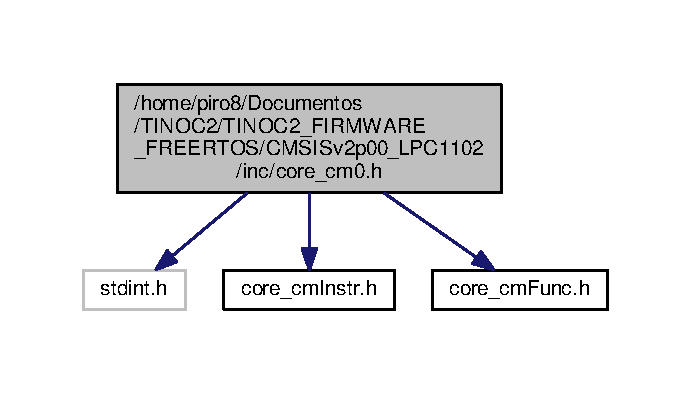
\includegraphics[width=332pt]{core__cm0_8h__incl}
\end{center}
\end{figure}
This graph shows which files directly or indirectly include this file\+:\nopagebreak
\begin{figure}[H]
\begin{center}
\leavevmode
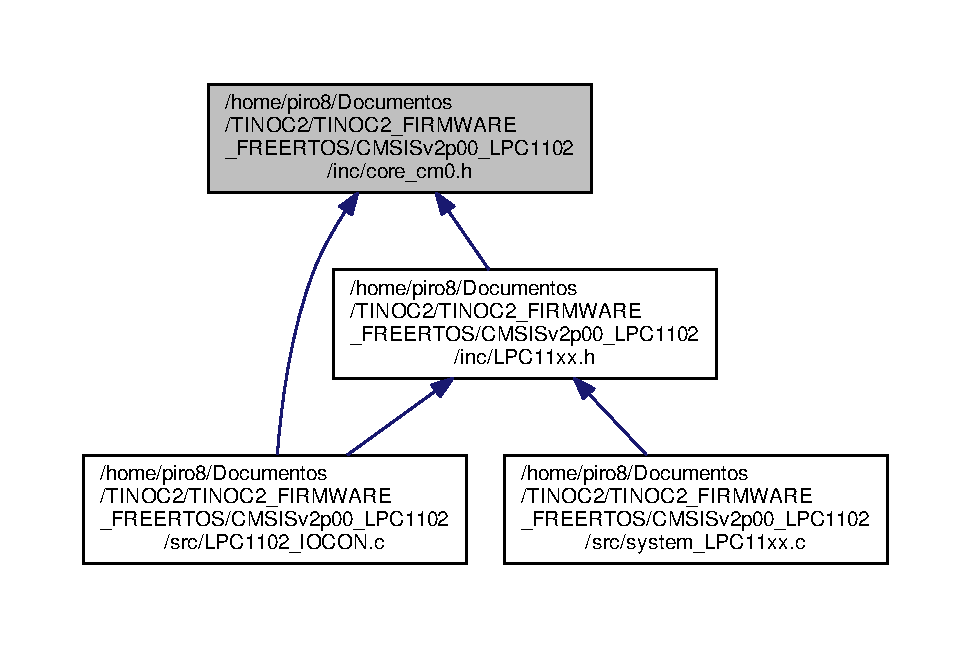
\includegraphics[width=350pt]{core__cm0_8h__dep__incl}
\end{center}
\end{figure}
\subsection*{Classes}
\begin{DoxyCompactItemize}
\item 
union \hyperlink{union_a_p_s_r___type}{A\+P\+S\+R\+\_\+\+Type}
\begin{DoxyCompactList}\small\item\em Union type to access the Application Program Status Register (A\+P\+SR). \end{DoxyCompactList}\item 
union \hyperlink{union_i_p_s_r___type}{I\+P\+S\+R\+\_\+\+Type}
\begin{DoxyCompactList}\small\item\em Union type to access the Interrupt Program Status Register (I\+P\+SR). \end{DoxyCompactList}\item 
union \hyperlink{unionx_p_s_r___type}{x\+P\+S\+R\+\_\+\+Type}
\begin{DoxyCompactList}\small\item\em Union type to access the Special-\/\+Purpose Program Status Registers (x\+P\+SR). \end{DoxyCompactList}\item 
union \hyperlink{union_c_o_n_t_r_o_l___type}{C\+O\+N\+T\+R\+O\+L\+\_\+\+Type}
\begin{DoxyCompactList}\small\item\em Union type to access the Control Registers (C\+O\+N\+T\+R\+OL). \end{DoxyCompactList}\item 
struct \hyperlink{struct_n_v_i_c___type}{N\+V\+I\+C\+\_\+\+Type}
\begin{DoxyCompactList}\small\item\em Structure type to access the Nested Vectored Interrupt Controller (N\+V\+IC). \end{DoxyCompactList}\item 
struct \hyperlink{struct_s_c_b___type}{S\+C\+B\+\_\+\+Type}
\begin{DoxyCompactList}\small\item\em Structure type to access the System Control Block (S\+CB). \end{DoxyCompactList}\item 
struct \hyperlink{struct_sys_tick___type}{Sys\+Tick\+\_\+\+Type}
\begin{DoxyCompactList}\small\item\em Structure type to access the System Timer (Sys\+Tick). \end{DoxyCompactList}\end{DoxyCompactItemize}
\subsection*{Macros}
\begin{DoxyCompactItemize}
\item 
\#define \hyperlink{core__cm0_8h_a1c7b83f58ef7b4d6b5f50ec1e294b34e}{\+\_\+\+\_\+\+C\+O\+R\+E\+\_\+\+C\+M0\+\_\+\+H\+\_\+\+G\+E\+N\+E\+R\+IC}
\item 
\#define \hyperlink{group___c_m_s_i_s__core__definitions_gacd01bf0a654a7f15f606593aa636bc72}{\+\_\+\+\_\+\+C\+M0\+\_\+\+C\+M\+S\+I\+S\+\_\+\+V\+E\+R\+S\+I\+O\+N\+\_\+\+M\+A\+IN}~(0x02)
\item 
\#define \hyperlink{group___c_m_s_i_s__core__definitions_gab6a85b0d3b2fbcfb62003006ece175cc}{\+\_\+\+\_\+\+C\+M0\+\_\+\+C\+M\+S\+I\+S\+\_\+\+V\+E\+R\+S\+I\+O\+N\+\_\+\+S\+UB}~(0x00)
\item 
\#define \hyperlink{group___c_m_s_i_s__core__definitions_gaf233a7b7b2818cc6194e7a9386faccd8}{\+\_\+\+\_\+\+C\+M0\+\_\+\+C\+M\+S\+I\+S\+\_\+\+V\+E\+R\+S\+I\+ON}~((\hyperlink{group___c_m_s_i_s__core__definitions_gacd01bf0a654a7f15f606593aa636bc72}{\+\_\+\+\_\+\+C\+M0\+\_\+\+C\+M\+S\+I\+S\+\_\+\+V\+E\+R\+S\+I\+O\+N\+\_\+\+M\+A\+IN} $<$$<$ 16) $\vert$ \hyperlink{group___c_m_s_i_s__core__definitions_gab6a85b0d3b2fbcfb62003006ece175cc}{\+\_\+\+\_\+\+C\+M0\+\_\+\+C\+M\+S\+I\+S\+\_\+\+V\+E\+R\+S\+I\+O\+N\+\_\+\+S\+UB})
\item 
\#define \hyperlink{group___c_m_s_i_s__core__definitions_ga63ea62503c88acab19fcf3d5743009e3}{\+\_\+\+\_\+\+C\+O\+R\+T\+E\+X\+\_\+M}~(0x00)
\item 
\#define \hyperlink{group___c_m_s_i_s__core__definitions_gac1e2acb34ba7f2543bcb2249bead4aee}{\+\_\+\+\_\+\+C\+O\+R\+E\+\_\+\+C\+M0\+\_\+\+H\+\_\+\+D\+E\+P\+E\+N\+D\+A\+NT}
\item 
\#define \hyperlink{group___c_m_s_i_s__core__definitions_gaf63697ed9952cc71e1225efe205f6cd3}{\+\_\+\+\_\+I}~volatile const
\item 
\#define \hyperlink{group___c_m_s_i_s__core__definitions_ga7e25d9380f9ef903923964322e71f2f6}{\+\_\+\+\_\+O}~volatile
\item 
\#define \hyperlink{group___c_m_s_i_s__core__definitions_gaec43007d9998a0a0e01faede4133d6be}{\+\_\+\+\_\+\+IO}~volatile
\item 
\#define \hyperlink{group___c_m_s_i_s___s_c_b_ga58686b88f94f789d4e6f429fe1ff58cf}{S\+C\+B\+\_\+\+C\+P\+U\+I\+D\+\_\+\+I\+M\+P\+L\+E\+M\+E\+N\+T\+E\+R\+\_\+\+Pos}~24
\item 
\#define \hyperlink{group___c_m_s_i_s___s_c_b_ga0932b31faafd47656a03ced75a31d99b}{S\+C\+B\+\_\+\+C\+P\+U\+I\+D\+\_\+\+I\+M\+P\+L\+E\+M\+E\+N\+T\+E\+R\+\_\+\+Msk}~(0x\+F\+F\+U\+L $<$$<$ S\+C\+B\+\_\+\+C\+P\+U\+I\+D\+\_\+\+I\+M\+P\+L\+E\+M\+E\+N\+T\+E\+R\+\_\+\+Pos)
\item 
\#define \hyperlink{group___c_m_s_i_s___s_c_b_ga104462bd0815391b4044a70bd15d3a71}{S\+C\+B\+\_\+\+C\+P\+U\+I\+D\+\_\+\+V\+A\+R\+I\+A\+N\+T\+\_\+\+Pos}~20
\item 
\#define \hyperlink{group___c_m_s_i_s___s_c_b_gad358dfbd04300afc1824329d128b99e8}{S\+C\+B\+\_\+\+C\+P\+U\+I\+D\+\_\+\+V\+A\+R\+I\+A\+N\+T\+\_\+\+Msk}~(0x\+F\+U\+L $<$$<$ S\+C\+B\+\_\+\+C\+P\+U\+I\+D\+\_\+\+V\+A\+R\+I\+A\+N\+T\+\_\+\+Pos)
\item 
\#define \hyperlink{group___c_m_s_i_s___s_c_b_gaf8b3236b08fb8e840efb682645fb0e98}{S\+C\+B\+\_\+\+C\+P\+U\+I\+D\+\_\+\+A\+R\+C\+H\+I\+T\+E\+C\+T\+U\+R\+E\+\_\+\+Pos}~16
\item 
\#define \hyperlink{group___c_m_s_i_s___s_c_b_gafae4a1f27a927338ae9dc51a0e146213}{S\+C\+B\+\_\+\+C\+P\+U\+I\+D\+\_\+\+A\+R\+C\+H\+I\+T\+E\+C\+T\+U\+R\+E\+\_\+\+Msk}~(0x\+F\+U\+L $<$$<$ S\+C\+B\+\_\+\+C\+P\+U\+I\+D\+\_\+\+A\+R\+C\+H\+I\+T\+E\+C\+T\+U\+R\+E\+\_\+\+Pos)
\item 
\#define \hyperlink{group___c_m_s_i_s___s_c_b_ga705f68eaa9afb042ca2407dc4e4629ac}{S\+C\+B\+\_\+\+C\+P\+U\+I\+D\+\_\+\+P\+A\+R\+T\+N\+O\+\_\+\+Pos}~4
\item 
\#define \hyperlink{group___c_m_s_i_s___s_c_b_ga98e581423ca016680c238c469aba546d}{S\+C\+B\+\_\+\+C\+P\+U\+I\+D\+\_\+\+P\+A\+R\+T\+N\+O\+\_\+\+Msk}~(0x\+F\+F\+F\+U\+L $<$$<$ S\+C\+B\+\_\+\+C\+P\+U\+I\+D\+\_\+\+P\+A\+R\+T\+N\+O\+\_\+\+Pos)
\item 
\#define \hyperlink{group___c_m_s_i_s___s_c_b_ga3c3d9071e574de11fb27ba57034838b1}{S\+C\+B\+\_\+\+C\+P\+U\+I\+D\+\_\+\+R\+E\+V\+I\+S\+I\+O\+N\+\_\+\+Pos}~0
\item 
\#define \hyperlink{group___c_m_s_i_s___s_c_b_ga2ec0448b6483f77e7f5d08b4b81d85df}{S\+C\+B\+\_\+\+C\+P\+U\+I\+D\+\_\+\+R\+E\+V\+I\+S\+I\+O\+N\+\_\+\+Msk}~(0x\+F\+U\+L $<$$<$ S\+C\+B\+\_\+\+C\+P\+U\+I\+D\+\_\+\+R\+E\+V\+I\+S\+I\+O\+N\+\_\+\+Pos)
\item 
\#define \hyperlink{group___c_m_s_i_s___s_c_b_ga750d4b52624a46d71356db4ea769573b}{S\+C\+B\+\_\+\+I\+C\+S\+R\+\_\+\+N\+M\+I\+P\+E\+N\+D\+S\+E\+T\+\_\+\+Pos}~31
\item 
\#define \hyperlink{group___c_m_s_i_s___s_c_b_ga340e3f79e9c3607dee9f2c048b6b22e8}{S\+C\+B\+\_\+\+I\+C\+S\+R\+\_\+\+N\+M\+I\+P\+E\+N\+D\+S\+E\+T\+\_\+\+Msk}~(1\+U\+L $<$$<$ S\+C\+B\+\_\+\+I\+C\+S\+R\+\_\+\+N\+M\+I\+P\+E\+N\+D\+S\+E\+T\+\_\+\+Pos)
\item 
\#define \hyperlink{group___c_m_s_i_s___s_c_b_gab5ded23d2ab1d5ff7cc7ce746205e9fe}{S\+C\+B\+\_\+\+I\+C\+S\+R\+\_\+\+P\+E\+N\+D\+S\+V\+S\+E\+T\+\_\+\+Pos}~28
\item 
\#define \hyperlink{group___c_m_s_i_s___s_c_b_ga1e40d93efb402763c8c00ddcc56724ff}{S\+C\+B\+\_\+\+I\+C\+S\+R\+\_\+\+P\+E\+N\+D\+S\+V\+S\+E\+T\+\_\+\+Msk}~(1\+U\+L $<$$<$ S\+C\+B\+\_\+\+I\+C\+S\+R\+\_\+\+P\+E\+N\+D\+S\+V\+S\+E\+T\+\_\+\+Pos)
\item 
\#define \hyperlink{group___c_m_s_i_s___s_c_b_gae218d9022288f89faf57187c4d542ecd}{S\+C\+B\+\_\+\+I\+C\+S\+R\+\_\+\+P\+E\+N\+D\+S\+V\+C\+L\+R\+\_\+\+Pos}~27
\item 
\#define \hyperlink{group___c_m_s_i_s___s_c_b_ga4a901ace381d3c1c74ac82b22fae2e1e}{S\+C\+B\+\_\+\+I\+C\+S\+R\+\_\+\+P\+E\+N\+D\+S\+V\+C\+L\+R\+\_\+\+Msk}~(1\+U\+L $<$$<$ S\+C\+B\+\_\+\+I\+C\+S\+R\+\_\+\+P\+E\+N\+D\+S\+V\+C\+L\+R\+\_\+\+Pos)
\item 
\#define \hyperlink{group___c_m_s_i_s___s_c_b_ga9dbb3358c6167c9c3f85661b90fb2794}{S\+C\+B\+\_\+\+I\+C\+S\+R\+\_\+\+P\+E\+N\+D\+S\+T\+S\+E\+T\+\_\+\+Pos}~26
\item 
\#define \hyperlink{group___c_m_s_i_s___s_c_b_ga7325b61ea0ec323ef2d5c893b112e546}{S\+C\+B\+\_\+\+I\+C\+S\+R\+\_\+\+P\+E\+N\+D\+S\+T\+S\+E\+T\+\_\+\+Msk}~(1\+U\+L $<$$<$ S\+C\+B\+\_\+\+I\+C\+S\+R\+\_\+\+P\+E\+N\+D\+S\+T\+S\+E\+T\+\_\+\+Pos)
\item 
\#define \hyperlink{group___c_m_s_i_s___s_c_b_gadbe25e4b333ece1341beb1a740168fdc}{S\+C\+B\+\_\+\+I\+C\+S\+R\+\_\+\+P\+E\+N\+D\+S\+T\+C\+L\+R\+\_\+\+Pos}~25
\item 
\#define \hyperlink{group___c_m_s_i_s___s_c_b_gab241827d2a793269d8cd99b9b28c2157}{S\+C\+B\+\_\+\+I\+C\+S\+R\+\_\+\+P\+E\+N\+D\+S\+T\+C\+L\+R\+\_\+\+Msk}~(1\+U\+L $<$$<$ S\+C\+B\+\_\+\+I\+C\+S\+R\+\_\+\+P\+E\+N\+D\+S\+T\+C\+L\+R\+\_\+\+Pos)
\item 
\#define \hyperlink{group___c_m_s_i_s___s_c_b_ga11cb5b1f9ce167b81f31787a77e575df}{S\+C\+B\+\_\+\+I\+C\+S\+R\+\_\+\+I\+S\+R\+P\+R\+E\+E\+M\+P\+T\+\_\+\+Pos}~23
\item 
\#define \hyperlink{group___c_m_s_i_s___s_c_b_gaa966600396290808d596fe96e92ca2b5}{S\+C\+B\+\_\+\+I\+C\+S\+R\+\_\+\+I\+S\+R\+P\+R\+E\+E\+M\+P\+T\+\_\+\+Msk}~(1\+U\+L $<$$<$ S\+C\+B\+\_\+\+I\+C\+S\+R\+\_\+\+I\+S\+R\+P\+R\+E\+E\+M\+P\+T\+\_\+\+Pos)
\item 
\#define \hyperlink{group___c_m_s_i_s___s_c_b_ga10749d92b9b744094b845c2eb46d4319}{S\+C\+B\+\_\+\+I\+C\+S\+R\+\_\+\+I\+S\+R\+P\+E\+N\+D\+I\+N\+G\+\_\+\+Pos}~22
\item 
\#define \hyperlink{group___c_m_s_i_s___s_c_b_ga056d74fd538e5d36d3be1f28d399c877}{S\+C\+B\+\_\+\+I\+C\+S\+R\+\_\+\+I\+S\+R\+P\+E\+N\+D\+I\+N\+G\+\_\+\+Msk}~(1\+U\+L $<$$<$ S\+C\+B\+\_\+\+I\+C\+S\+R\+\_\+\+I\+S\+R\+P\+E\+N\+D\+I\+N\+G\+\_\+\+Pos)
\item 
\#define \hyperlink{group___c_m_s_i_s___s_c_b_gada60c92bf88d6fd21a8f49efa4a127b8}{S\+C\+B\+\_\+\+I\+C\+S\+R\+\_\+\+V\+E\+C\+T\+P\+E\+N\+D\+I\+N\+G\+\_\+\+Pos}~12
\item 
\#define \hyperlink{group___c_m_s_i_s___s_c_b_gacb6992e7c7ddc27a370f62878a21ef72}{S\+C\+B\+\_\+\+I\+C\+S\+R\+\_\+\+V\+E\+C\+T\+P\+E\+N\+D\+I\+N\+G\+\_\+\+Msk}~(0x1\+F\+F\+U\+L $<$$<$ S\+C\+B\+\_\+\+I\+C\+S\+R\+\_\+\+V\+E\+C\+T\+P\+E\+N\+D\+I\+N\+G\+\_\+\+Pos)
\item 
\#define \hyperlink{group___c_m_s_i_s___s_c_b_gae4f602c7c5c895d5fb687b71b0979fc3}{S\+C\+B\+\_\+\+I\+C\+S\+R\+\_\+\+V\+E\+C\+T\+A\+C\+T\+I\+V\+E\+\_\+\+Pos}~0
\item 
\#define \hyperlink{group___c_m_s_i_s___s_c_b_ga5533791a4ecf1b9301c883047b3e8396}{S\+C\+B\+\_\+\+I\+C\+S\+R\+\_\+\+V\+E\+C\+T\+A\+C\+T\+I\+V\+E\+\_\+\+Msk}~(0x1\+F\+F\+U\+L $<$$<$ S\+C\+B\+\_\+\+I\+C\+S\+R\+\_\+\+V\+E\+C\+T\+A\+C\+T\+I\+V\+E\+\_\+\+Pos)
\item 
\#define \hyperlink{group___c_m_s_i_s___s_c_b_gaaa27c0ba600bf82c3da08c748845b640}{S\+C\+B\+\_\+\+A\+I\+R\+C\+R\+\_\+\+V\+E\+C\+T\+K\+E\+Y\+\_\+\+Pos}~16
\item 
\#define \hyperlink{group___c_m_s_i_s___s_c_b_ga90c7cf0c490e7ae55f9503a7fda1dd22}{S\+C\+B\+\_\+\+A\+I\+R\+C\+R\+\_\+\+V\+E\+C\+T\+K\+E\+Y\+\_\+\+Msk}~(0x\+F\+F\+F\+F\+U\+L $<$$<$ S\+C\+B\+\_\+\+A\+I\+R\+C\+R\+\_\+\+V\+E\+C\+T\+K\+E\+Y\+\_\+\+Pos)
\item 
\#define \hyperlink{group___c_m_s_i_s___s_c_b_gaec404750ff5ca07f499a3c06b62051ef}{S\+C\+B\+\_\+\+A\+I\+R\+C\+R\+\_\+\+V\+E\+C\+T\+K\+E\+Y\+S\+T\+A\+T\+\_\+\+Pos}~16
\item 
\#define \hyperlink{group___c_m_s_i_s___s_c_b_gabacedaefeefc73d666bbe59ece904493}{S\+C\+B\+\_\+\+A\+I\+R\+C\+R\+\_\+\+V\+E\+C\+T\+K\+E\+Y\+S\+T\+A\+T\+\_\+\+Msk}~(0x\+F\+F\+F\+F\+U\+L $<$$<$ S\+C\+B\+\_\+\+A\+I\+R\+C\+R\+\_\+\+V\+E\+C\+T\+K\+E\+Y\+S\+T\+A\+T\+\_\+\+Pos)
\item 
\#define \hyperlink{group___c_m_s_i_s___s_c_b_gad31dec98fbc0d33ace63cb1f1a927923}{S\+C\+B\+\_\+\+A\+I\+R\+C\+R\+\_\+\+E\+N\+D\+I\+A\+N\+E\+S\+S\+\_\+\+Pos}~15
\item 
\#define \hyperlink{group___c_m_s_i_s___s_c_b_ga2f571f93d3d4a6eac9a3040756d3d951}{S\+C\+B\+\_\+\+A\+I\+R\+C\+R\+\_\+\+E\+N\+D\+I\+A\+N\+E\+S\+S\+\_\+\+Msk}~(1\+U\+L $<$$<$ S\+C\+B\+\_\+\+A\+I\+R\+C\+R\+\_\+\+E\+N\+D\+I\+A\+N\+E\+S\+S\+\_\+\+Pos)
\item 
\#define \hyperlink{group___c_m_s_i_s___s_c_b_gaffb2737eca1eac0fc1c282a76a40953c}{S\+C\+B\+\_\+\+A\+I\+R\+C\+R\+\_\+\+S\+Y\+S\+R\+E\+S\+E\+T\+R\+E\+Q\+\_\+\+Pos}~2
\item 
\#define \hyperlink{group___c_m_s_i_s___s_c_b_gaae1181119559a5bd36e62afa373fa720}{S\+C\+B\+\_\+\+A\+I\+R\+C\+R\+\_\+\+S\+Y\+S\+R\+E\+S\+E\+T\+R\+E\+Q\+\_\+\+Msk}~(1\+U\+L $<$$<$ S\+C\+B\+\_\+\+A\+I\+R\+C\+R\+\_\+\+S\+Y\+S\+R\+E\+S\+E\+T\+R\+E\+Q\+\_\+\+Pos)
\item 
\#define \hyperlink{group___c_m_s_i_s___s_c_b_gaa30a12e892bb696e61626d71359a9029}{S\+C\+B\+\_\+\+A\+I\+R\+C\+R\+\_\+\+V\+E\+C\+T\+C\+L\+R\+A\+C\+T\+I\+V\+E\+\_\+\+Pos}~1
\item 
\#define \hyperlink{group___c_m_s_i_s___s_c_b_ga212c5ab1c1c82c807d30d2307aa8d218}{S\+C\+B\+\_\+\+A\+I\+R\+C\+R\+\_\+\+V\+E\+C\+T\+C\+L\+R\+A\+C\+T\+I\+V\+E\+\_\+\+Msk}~(1\+U\+L $<$$<$ S\+C\+B\+\_\+\+A\+I\+R\+C\+R\+\_\+\+V\+E\+C\+T\+C\+L\+R\+A\+C\+T\+I\+V\+E\+\_\+\+Pos)
\item 
\#define \hyperlink{group___c_m_s_i_s___s_c_b_ga3bddcec40aeaf3d3a998446100fa0e44}{S\+C\+B\+\_\+\+S\+C\+R\+\_\+\+S\+E\+V\+O\+N\+P\+E\+N\+D\+\_\+\+Pos}~4
\item 
\#define \hyperlink{group___c_m_s_i_s___s_c_b_gafb98656644a14342e467505f69a997c9}{S\+C\+B\+\_\+\+S\+C\+R\+\_\+\+S\+E\+V\+O\+N\+P\+E\+N\+D\+\_\+\+Msk}~(1\+U\+L $<$$<$ S\+C\+B\+\_\+\+S\+C\+R\+\_\+\+S\+E\+V\+O\+N\+P\+E\+N\+D\+\_\+\+Pos)
\item 
\#define \hyperlink{group___c_m_s_i_s___s_c_b_gab304f6258ec03bd9a6e7a360515c3cfe}{S\+C\+B\+\_\+\+S\+C\+R\+\_\+\+S\+L\+E\+E\+P\+D\+E\+E\+P\+\_\+\+Pos}~2
\item 
\#define \hyperlink{group___c_m_s_i_s___s_c_b_ga77c06a69c63f4b3f6ec1032e911e18e7}{S\+C\+B\+\_\+\+S\+C\+R\+\_\+\+S\+L\+E\+E\+P\+D\+E\+E\+P\+\_\+\+Msk}~(1\+U\+L $<$$<$ S\+C\+B\+\_\+\+S\+C\+R\+\_\+\+S\+L\+E\+E\+P\+D\+E\+E\+P\+\_\+\+Pos)
\item 
\#define \hyperlink{group___c_m_s_i_s___s_c_b_ga3680a15114d7fdc1e25043b881308fe9}{S\+C\+B\+\_\+\+S\+C\+R\+\_\+\+S\+L\+E\+E\+P\+O\+N\+E\+X\+I\+T\+\_\+\+Pos}~1
\item 
\#define \hyperlink{group___c_m_s_i_s___s_c_b_ga50a243e317b9a70781b02758d45b05ee}{S\+C\+B\+\_\+\+S\+C\+R\+\_\+\+S\+L\+E\+E\+P\+O\+N\+E\+X\+I\+T\+\_\+\+Msk}~(1\+U\+L $<$$<$ S\+C\+B\+\_\+\+S\+C\+R\+\_\+\+S\+L\+E\+E\+P\+O\+N\+E\+X\+I\+T\+\_\+\+Pos)
\item 
\#define \hyperlink{group___c_m_s_i_s___s_c_b_gac2d20a250960a432cc74da59d20e2f86}{S\+C\+B\+\_\+\+C\+C\+R\+\_\+\+S\+T\+K\+A\+L\+I\+G\+N\+\_\+\+Pos}~9
\item 
\#define \hyperlink{group___c_m_s_i_s___s_c_b_ga33cf22d3d46af158a03aad25ddea1bcb}{S\+C\+B\+\_\+\+C\+C\+R\+\_\+\+S\+T\+K\+A\+L\+I\+G\+N\+\_\+\+Msk}~(1\+U\+L $<$$<$ S\+C\+B\+\_\+\+C\+C\+R\+\_\+\+S\+T\+K\+A\+L\+I\+G\+N\+\_\+\+Pos)
\item 
\#define \hyperlink{group___c_m_s_i_s___s_c_b_gac4e4928b864ea10fc24dbbc57d976229}{S\+C\+B\+\_\+\+C\+C\+R\+\_\+\+U\+N\+A\+L\+I\+G\+N\+\_\+\+T\+R\+P\+\_\+\+Pos}~3
\item 
\#define \hyperlink{group___c_m_s_i_s___s_c_b_ga68c96ad594af70c007923979085c99e0}{S\+C\+B\+\_\+\+C\+C\+R\+\_\+\+U\+N\+A\+L\+I\+G\+N\+\_\+\+T\+R\+P\+\_\+\+Msk}~(1\+U\+L $<$$<$ S\+C\+B\+\_\+\+C\+C\+R\+\_\+\+U\+N\+A\+L\+I\+G\+N\+\_\+\+T\+R\+P\+\_\+\+Pos)
\item 
\#define \hyperlink{group___c_m_s_i_s___sys_tick_gadbb65d4a815759649db41df216ed4d60}{Sys\+Tick\+\_\+\+C\+T\+R\+L\+\_\+\+C\+O\+U\+N\+T\+F\+L\+A\+G\+\_\+\+Pos}~16
\item 
\#define \hyperlink{group___c_m_s_i_s___sys_tick_ga1bf3033ecccf200f59baefe15dbb367c}{Sys\+Tick\+\_\+\+C\+T\+R\+L\+\_\+\+C\+O\+U\+N\+T\+F\+L\+A\+G\+\_\+\+Msk}~(1\+U\+L $<$$<$ Sys\+Tick\+\_\+\+C\+T\+R\+L\+\_\+\+C\+O\+U\+N\+T\+F\+L\+A\+G\+\_\+\+Pos)
\item 
\#define \hyperlink{group___c_m_s_i_s___sys_tick_ga24fbc69a5f0b78d67fda2300257baff1}{Sys\+Tick\+\_\+\+C\+T\+R\+L\+\_\+\+C\+L\+K\+S\+O\+U\+R\+C\+E\+\_\+\+Pos}~2
\item 
\#define \hyperlink{group___c_m_s_i_s___sys_tick_gaa41d06039797423a46596bd313d57373}{Sys\+Tick\+\_\+\+C\+T\+R\+L\+\_\+\+C\+L\+K\+S\+O\+U\+R\+C\+E\+\_\+\+Msk}~(1\+U\+L $<$$<$ Sys\+Tick\+\_\+\+C\+T\+R\+L\+\_\+\+C\+L\+K\+S\+O\+U\+R\+C\+E\+\_\+\+Pos)
\item 
\#define \hyperlink{group___c_m_s_i_s___sys_tick_ga88f45bbb89ce8df3cd2b2613c7b48214}{Sys\+Tick\+\_\+\+C\+T\+R\+L\+\_\+\+T\+I\+C\+K\+I\+N\+T\+\_\+\+Pos}~1
\item 
\#define \hyperlink{group___c_m_s_i_s___sys_tick_ga95bb984266ca764024836a870238a027}{Sys\+Tick\+\_\+\+C\+T\+R\+L\+\_\+\+T\+I\+C\+K\+I\+N\+T\+\_\+\+Msk}~(1\+U\+L $<$$<$ Sys\+Tick\+\_\+\+C\+T\+R\+L\+\_\+\+T\+I\+C\+K\+I\+N\+T\+\_\+\+Pos)
\item 
\#define \hyperlink{group___c_m_s_i_s___sys_tick_ga0b48cc1e36d92a92e4bf632890314810}{Sys\+Tick\+\_\+\+C\+T\+R\+L\+\_\+\+E\+N\+A\+B\+L\+E\+\_\+\+Pos}~0
\item 
\#define \hyperlink{group___c_m_s_i_s___sys_tick_ga16c9fee0ed0235524bdeb38af328fd1f}{Sys\+Tick\+\_\+\+C\+T\+R\+L\+\_\+\+E\+N\+A\+B\+L\+E\+\_\+\+Msk}~(1\+U\+L $<$$<$ Sys\+Tick\+\_\+\+C\+T\+R\+L\+\_\+\+E\+N\+A\+B\+L\+E\+\_\+\+Pos)
\item 
\#define \hyperlink{group___c_m_s_i_s___sys_tick_gaf44d10df359dc5bf5752b0894ae3bad2}{Sys\+Tick\+\_\+\+L\+O\+A\+D\+\_\+\+R\+E\+L\+O\+A\+D\+\_\+\+Pos}~0
\item 
\#define \hyperlink{group___c_m_s_i_s___sys_tick_ga265912a7962f0e1abd170336e579b1b1}{Sys\+Tick\+\_\+\+L\+O\+A\+D\+\_\+\+R\+E\+L\+O\+A\+D\+\_\+\+Msk}~(0x\+F\+F\+F\+F\+F\+F\+U\+L $<$$<$ Sys\+Tick\+\_\+\+L\+O\+A\+D\+\_\+\+R\+E\+L\+O\+A\+D\+\_\+\+Pos)
\item 
\#define \hyperlink{group___c_m_s_i_s___sys_tick_ga3208104c3b019b5de35ae8c21d5c34dd}{Sys\+Tick\+\_\+\+V\+A\+L\+\_\+\+C\+U\+R\+R\+E\+N\+T\+\_\+\+Pos}~0
\item 
\#define \hyperlink{group___c_m_s_i_s___sys_tick_gafc77b56d568930b49a2474debc75ab45}{Sys\+Tick\+\_\+\+V\+A\+L\+\_\+\+C\+U\+R\+R\+E\+N\+T\+\_\+\+Msk}~(0x\+F\+F\+F\+F\+F\+F\+U\+L $<$$<$ Sys\+Tick\+\_\+\+V\+A\+L\+\_\+\+C\+U\+R\+R\+E\+N\+T\+\_\+\+Pos)
\item 
\#define \hyperlink{group___c_m_s_i_s___sys_tick_ga534dbe414e7a46a6ce4c1eca1fbff409}{Sys\+Tick\+\_\+\+C\+A\+L\+I\+B\+\_\+\+N\+O\+R\+E\+F\+\_\+\+Pos}~31
\item 
\#define \hyperlink{group___c_m_s_i_s___sys_tick_ga3af0d891fdd99bcc8d8912d37830edb6}{Sys\+Tick\+\_\+\+C\+A\+L\+I\+B\+\_\+\+N\+O\+R\+E\+F\+\_\+\+Msk}~(1\+U\+L $<$$<$ Sys\+Tick\+\_\+\+C\+A\+L\+I\+B\+\_\+\+N\+O\+R\+E\+F\+\_\+\+Pos)
\item 
\#define \hyperlink{group___c_m_s_i_s___sys_tick_gadd0c9cd6641b9f6a0c618e7982954860}{Sys\+Tick\+\_\+\+C\+A\+L\+I\+B\+\_\+\+S\+K\+E\+W\+\_\+\+Pos}~30
\item 
\#define \hyperlink{group___c_m_s_i_s___sys_tick_ga8a6a85a87334776f33d77fd147587431}{Sys\+Tick\+\_\+\+C\+A\+L\+I\+B\+\_\+\+S\+K\+E\+W\+\_\+\+Msk}~(1\+U\+L $<$$<$ Sys\+Tick\+\_\+\+C\+A\+L\+I\+B\+\_\+\+S\+K\+E\+W\+\_\+\+Pos)
\item 
\#define \hyperlink{group___c_m_s_i_s___sys_tick_gacae558f6e75a0bed5d826f606d8e695e}{Sys\+Tick\+\_\+\+C\+A\+L\+I\+B\+\_\+\+T\+E\+N\+M\+S\+\_\+\+Pos}~0
\item 
\#define \hyperlink{group___c_m_s_i_s___sys_tick_gaf1e68865c5aece2ad58971225bd3e95e}{Sys\+Tick\+\_\+\+C\+A\+L\+I\+B\+\_\+\+T\+E\+N\+M\+S\+\_\+\+Msk}~(0x\+F\+F\+F\+F\+F\+F\+U\+L $<$$<$ Sys\+Tick\+\_\+\+V\+A\+L\+\_\+\+C\+U\+R\+R\+E\+N\+T\+\_\+\+Pos)
\item 
\#define \hyperlink{group___c_m_s_i_s___core___n_v_i_c_functions_ga53c75b28823441c6153269f0ecbed878}{\+\_\+\+B\+I\+T\+\_\+\+S\+H\+I\+FT}(\hyperlink{group___l_p_c11xx___c_m_s_i_s_ga666eb0caeb12ec0e281415592ae89083}{I\+R\+Qn})~(  (((uint32\+\_\+t)(\hyperlink{group___l_p_c11xx___c_m_s_i_s_ga666eb0caeb12ec0e281415592ae89083}{I\+R\+Qn})       )    \&  0x03) $\ast$ 8 )
\item 
\#define \hyperlink{group___c_m_s_i_s___core___n_v_i_c_functions_gaee4f7eb5d7e770ad51489dbceabb1755}{\+\_\+\+S\+H\+P\+\_\+\+I\+DX}(\hyperlink{group___l_p_c11xx___c_m_s_i_s_ga666eb0caeb12ec0e281415592ae89083}{I\+R\+Qn})~( ((((uint32\+\_\+t)(\hyperlink{group___l_p_c11xx___c_m_s_i_s_ga666eb0caeb12ec0e281415592ae89083}{I\+R\+Qn}) \& 0x0\+F)-\/8) $>$$>$    2)     )
\item 
\#define \hyperlink{group___c_m_s_i_s___core___n_v_i_c_functions_ga370ec4b1751a6a889d849747df3763a9}{\+\_\+\+I\+P\+\_\+\+I\+DX}(\hyperlink{group___l_p_c11xx___c_m_s_i_s_ga666eb0caeb12ec0e281415592ae89083}{I\+R\+Qn})~(   ((uint32\+\_\+t)(\hyperlink{group___l_p_c11xx___c_m_s_i_s_ga666eb0caeb12ec0e281415592ae89083}{I\+R\+Qn})            $>$$>$    2)     )
\end{DoxyCompactItemize}
{\bf }\par
\begin{DoxyCompactItemize}
\item 
\#define \hyperlink{group___c_m_s_i_s__core__register_ga3c14ed93192c8d9143322bbf77ebf770}{S\+C\+S\+\_\+\+B\+A\+SE}~(0x\+E000\+E000\+U\+L)
\item 
\#define \hyperlink{group___c_m_s_i_s__core__register_ga680604dbcda9e9b31a1639fcffe5230b}{Core\+Debug\+\_\+\+B\+A\+SE}~(0x\+E000\+E\+D\+F0\+U\+L)
\item 
\#define \hyperlink{group___c_m_s_i_s__core__register_ga58effaac0b93006b756d33209e814646}{Sys\+Tick\+\_\+\+B\+A\+SE}~(\hyperlink{group___c_m_s_i_s__core__register_ga3c14ed93192c8d9143322bbf77ebf770}{S\+C\+S\+\_\+\+B\+A\+SE} +  0x0010\+U\+L)
\item 
\#define \hyperlink{group___c_m_s_i_s__core__register_gaa0288691785a5f868238e0468b39523d}{N\+V\+I\+C\+\_\+\+B\+A\+SE}~(\hyperlink{group___c_m_s_i_s__core__register_ga3c14ed93192c8d9143322bbf77ebf770}{S\+C\+S\+\_\+\+B\+A\+SE} +  0x0100\+U\+L)
\item 
\#define \hyperlink{group___c_m_s_i_s__core__register_gad55a7ddb8d4b2398b0c1cfec76c0d9fd}{S\+C\+B\+\_\+\+B\+A\+SE}~(\hyperlink{group___c_m_s_i_s__core__register_ga3c14ed93192c8d9143322bbf77ebf770}{S\+C\+S\+\_\+\+B\+A\+SE} +  0x0\+D00\+U\+L)
\item 
\#define \hyperlink{group___c_m_s_i_s__core__register_gaaaf6477c2bde2f00f99e3c2fd1060b01}{S\+CB}~((\hyperlink{struct_s_c_b___type}{S\+C\+B\+\_\+\+Type} $\ast$)           \hyperlink{group___c_m_s_i_s__core__register_gad55a7ddb8d4b2398b0c1cfec76c0d9fd}{S\+C\+B\+\_\+\+B\+A\+SE})
\item 
\#define \hyperlink{group___c_m_s_i_s__core__register_gacd96c53beeaff8f603fcda425eb295de}{Sys\+Tick}~((\hyperlink{struct_sys_tick___type}{Sys\+Tick\+\_\+\+Type} $\ast$)       \hyperlink{group___c_m_s_i_s__core__register_ga58effaac0b93006b756d33209e814646}{Sys\+Tick\+\_\+\+B\+A\+SE})
\item 
\#define \hyperlink{group___c_m_s_i_s__core__register_gac8e97e8ce56ae9f57da1363a937f8a17}{N\+V\+IC}~((\hyperlink{struct_n_v_i_c___type}{N\+V\+I\+C\+\_\+\+Type} $\ast$)          \hyperlink{group___c_m_s_i_s__core__register_gaa0288691785a5f868238e0468b39523d}{N\+V\+I\+C\+\_\+\+B\+A\+SE})
\end{DoxyCompactItemize}



\subsection{Detailed Description}
C\+M\+S\+IS Cortex-\/\+M0 Core Peripheral Access Layer Header File. 

\begin{DoxyVersion}{Version}
V2.\+03 
\end{DoxyVersion}
\begin{DoxyDate}{Date}
23. May 2011
\end{DoxyDate}
\begin{DoxyNote}{Note}
Copyright (C) 2009-\/2011 A\+RM Limited. All rights reserved.
\end{DoxyNote}
\begin{DoxyParagraph}{}
A\+RM Limited (A\+RM) is supplying this software for use with Cortex-\/M processor based microcontrollers. This file can be freely distributed within development tools that are supporting such A\+RM based processors.
\end{DoxyParagraph}
\begin{DoxyParagraph}{}
T\+H\+IS S\+O\+F\+T\+W\+A\+RE IS P\+R\+O\+V\+I\+D\+ED \char`\"{}\+A\+S I\+S\char`\"{}. NO W\+A\+R\+R\+A\+N\+T\+I\+ES, W\+H\+E\+T\+H\+ER E\+X\+P\+R\+E\+SS, I\+M\+P\+L\+I\+ED OR S\+T\+A\+T\+U\+T\+O\+RY, I\+N\+C\+L\+U\+D\+I\+NG, B\+UT N\+OT L\+I\+M\+I\+T\+ED TO, I\+M\+P\+L\+I\+ED W\+A\+R\+R\+A\+N\+T\+I\+ES OF M\+E\+R\+C\+H\+A\+N\+T\+A\+B\+I\+L\+I\+TY A\+ND F\+I\+T\+N\+E\+SS F\+OR A P\+A\+R\+T\+I\+C\+U\+L\+AR P\+U\+R\+P\+O\+SE A\+P\+P\+LY TO T\+H\+IS S\+O\+F\+T\+W\+A\+RE. A\+RM S\+H\+A\+LL N\+OT, IN A\+NY C\+I\+R\+C\+U\+M\+S\+T\+A\+N\+C\+ES, BE L\+I\+A\+B\+LE F\+OR S\+P\+E\+C\+I\+AL, I\+N\+C\+I\+D\+E\+N\+T\+AL, OR C\+O\+N\+S\+E\+Q\+U\+E\+N\+T\+I\+AL D\+A\+M\+A\+G\+ES, F\+OR A\+NY R\+E\+A\+S\+ON W\+H\+A\+T\+S\+O\+E\+V\+ER. 
\end{DoxyParagraph}


\subsection{Macro Definition Documentation}
\index{core\+\_\+cm0.\+h@{core\+\_\+cm0.\+h}!\+\_\+\+\_\+\+C\+O\+R\+E\+\_\+\+C\+M0\+\_\+\+H\+\_\+\+G\+E\+N\+E\+R\+IC@{\+\_\+\+\_\+\+C\+O\+R\+E\+\_\+\+C\+M0\+\_\+\+H\+\_\+\+G\+E\+N\+E\+R\+IC}}
\index{\+\_\+\+\_\+\+C\+O\+R\+E\+\_\+\+C\+M0\+\_\+\+H\+\_\+\+G\+E\+N\+E\+R\+IC@{\+\_\+\+\_\+\+C\+O\+R\+E\+\_\+\+C\+M0\+\_\+\+H\+\_\+\+G\+E\+N\+E\+R\+IC}!core\+\_\+cm0.\+h@{core\+\_\+cm0.\+h}}
\subsubsection[{\texorpdfstring{\+\_\+\+\_\+\+C\+O\+R\+E\+\_\+\+C\+M0\+\_\+\+H\+\_\+\+G\+E\+N\+E\+R\+IC}{__CORE_CM0_H_GENERIC}}]{\setlength{\rightskip}{0pt plus 5cm}\#define \+\_\+\+\_\+\+C\+O\+R\+E\+\_\+\+C\+M0\+\_\+\+H\+\_\+\+G\+E\+N\+E\+R\+IC}\hypertarget{core__cm0_8h_a1c7b83f58ef7b4d6b5f50ec1e294b34e}{}\label{core__cm0_8h_a1c7b83f58ef7b4d6b5f50ec1e294b34e}


Definition at line 32 of file core\+\_\+cm0.\+h.


\hypertarget{core__cm_func_8h}{}\section{/home/piro8/\+Documentos/\+T\+I\+N\+O\+C2/\+T\+I\+N\+O\+C2\+\_\+\+F\+I\+R\+M\+W\+A\+R\+E\+\_\+\+F\+R\+E\+E\+R\+T\+O\+S/\+C\+M\+S\+I\+Sv2p00\+\_\+\+L\+P\+C1102/inc/core\+\_\+cm\+Func.h File Reference}
\label{core__cm_func_8h}\index{/home/piro8/\+Documentos/\+T\+I\+N\+O\+C2/\+T\+I\+N\+O\+C2\+\_\+\+F\+I\+R\+M\+W\+A\+R\+E\+\_\+\+F\+R\+E\+E\+R\+T\+O\+S/\+C\+M\+S\+I\+Sv2p00\+\_\+\+L\+P\+C1102/inc/core\+\_\+cm\+Func.\+h@{/home/piro8/\+Documentos/\+T\+I\+N\+O\+C2/\+T\+I\+N\+O\+C2\+\_\+\+F\+I\+R\+M\+W\+A\+R\+E\+\_\+\+F\+R\+E\+E\+R\+T\+O\+S/\+C\+M\+S\+I\+Sv2p00\+\_\+\+L\+P\+C1102/inc/core\+\_\+cm\+Func.\+h}}


C\+M\+S\+IS Cortex-\/M Core Function Access Header File.  


This graph shows which files directly or indirectly include this file\+:\nopagebreak
\begin{figure}[H]
\begin{center}
\leavevmode
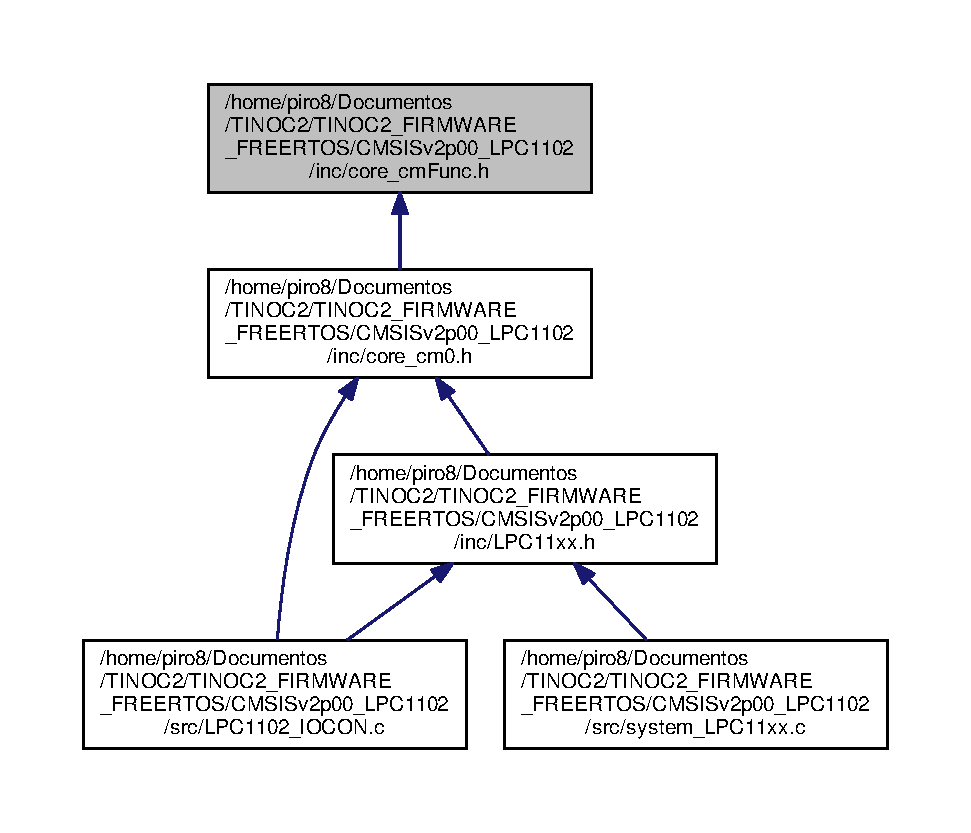
\includegraphics[width=350pt]{core__cm_func_8h__dep__incl}
\end{center}
\end{figure}


\subsection{Detailed Description}
C\+M\+S\+IS Cortex-\/M Core Function Access Header File. 

\begin{DoxyVersion}{Version}
V2.\+01 
\end{DoxyVersion}
\begin{DoxyDate}{Date}
06. December 2010
\end{DoxyDate}
\begin{DoxyNote}{Note}
Copyright (C) 2009-\/2010 A\+RM Limited. All rights reserved.
\end{DoxyNote}
\begin{DoxyParagraph}{}
A\+RM Limited (A\+RM) is supplying this software for use with Cortex-\/M processor based microcontrollers. This file can be freely distributed within development tools that are supporting such A\+RM based processors.
\end{DoxyParagraph}
\begin{DoxyParagraph}{}
T\+H\+IS S\+O\+F\+T\+W\+A\+RE IS P\+R\+O\+V\+I\+D\+ED \char`\"{}\+A\+S I\+S\char`\"{}. NO W\+A\+R\+R\+A\+N\+T\+I\+ES, W\+H\+E\+T\+H\+ER E\+X\+P\+R\+E\+SS, I\+M\+P\+L\+I\+ED OR S\+T\+A\+T\+U\+T\+O\+RY, I\+N\+C\+L\+U\+D\+I\+NG, B\+UT N\+OT L\+I\+M\+I\+T\+ED TO, I\+M\+P\+L\+I\+ED W\+A\+R\+R\+A\+N\+T\+I\+ES OF M\+E\+R\+C\+H\+A\+N\+T\+A\+B\+I\+L\+I\+TY A\+ND F\+I\+T\+N\+E\+SS F\+OR A P\+A\+R\+T\+I\+C\+U\+L\+AR P\+U\+R\+P\+O\+SE A\+P\+P\+LY TO T\+H\+IS S\+O\+F\+T\+W\+A\+RE. A\+RM S\+H\+A\+LL N\+OT, IN A\+NY C\+I\+R\+C\+U\+M\+S\+T\+A\+N\+C\+ES, BE L\+I\+A\+B\+LE F\+OR S\+P\+E\+C\+I\+AL, I\+N\+C\+I\+D\+E\+N\+T\+AL, OR C\+O\+N\+S\+E\+Q\+U\+E\+N\+T\+I\+AL D\+A\+M\+A\+G\+ES, F\+OR A\+NY R\+E\+A\+S\+ON W\+H\+A\+T\+S\+O\+E\+V\+ER. 
\end{DoxyParagraph}

\hypertarget{core__cm_instr_8h}{}\section{/home/piro8/\+Documentos/\+T\+I\+N\+O\+C2/\+T\+I\+N\+O\+C2\+\_\+\+F\+I\+R\+M\+W\+A\+R\+E\+\_\+\+F\+R\+E\+E\+R\+T\+O\+S/\+C\+M\+S\+I\+Sv2p00\+\_\+\+L\+P\+C1102/inc/core\+\_\+cm\+Instr.h File Reference}
\label{core__cm_instr_8h}\index{/home/piro8/\+Documentos/\+T\+I\+N\+O\+C2/\+T\+I\+N\+O\+C2\+\_\+\+F\+I\+R\+M\+W\+A\+R\+E\+\_\+\+F\+R\+E\+E\+R\+T\+O\+S/\+C\+M\+S\+I\+Sv2p00\+\_\+\+L\+P\+C1102/inc/core\+\_\+cm\+Instr.\+h@{/home/piro8/\+Documentos/\+T\+I\+N\+O\+C2/\+T\+I\+N\+O\+C2\+\_\+\+F\+I\+R\+M\+W\+A\+R\+E\+\_\+\+F\+R\+E\+E\+R\+T\+O\+S/\+C\+M\+S\+I\+Sv2p00\+\_\+\+L\+P\+C1102/inc/core\+\_\+cm\+Instr.\+h}}


C\+M\+S\+IS Cortex-\/M Core Instruction Access Header File.  


This graph shows which files directly or indirectly include this file\+:\nopagebreak
\begin{figure}[H]
\begin{center}
\leavevmode
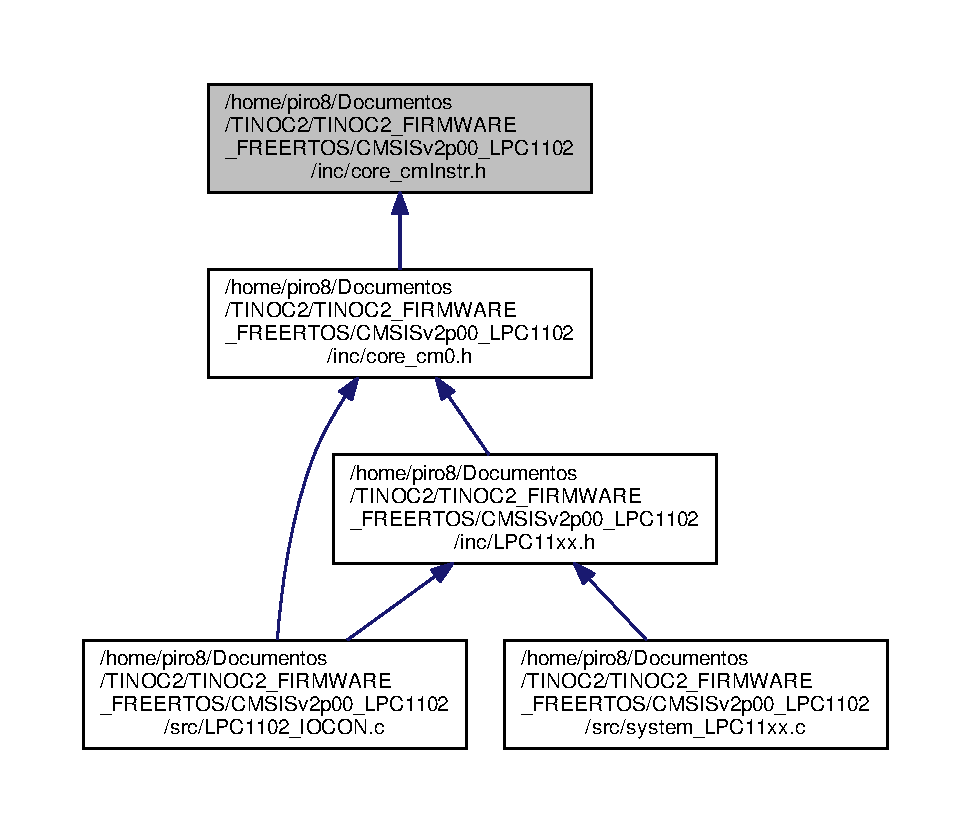
\includegraphics[width=350pt]{core__cm_instr_8h__dep__incl}
\end{center}
\end{figure}


\subsection{Detailed Description}
C\+M\+S\+IS Cortex-\/M Core Instruction Access Header File. 

\begin{DoxyVersion}{Version}
V2.\+01 
\end{DoxyVersion}
\begin{DoxyDate}{Date}
06. December 2010
\end{DoxyDate}
\begin{DoxyNote}{Note}
Copyright (C) 2009-\/2010 A\+RM Limited. All rights reserved.
\end{DoxyNote}
\begin{DoxyParagraph}{}
A\+RM Limited (A\+RM) is supplying this software for use with Cortex-\/M processor based microcontrollers. This file can be freely distributed within development tools that are supporting such A\+RM based processors.
\end{DoxyParagraph}
\begin{DoxyParagraph}{}
T\+H\+IS S\+O\+F\+T\+W\+A\+RE IS P\+R\+O\+V\+I\+D\+ED \char`\"{}\+A\+S I\+S\char`\"{}. NO W\+A\+R\+R\+A\+N\+T\+I\+ES, W\+H\+E\+T\+H\+ER E\+X\+P\+R\+E\+SS, I\+M\+P\+L\+I\+ED OR S\+T\+A\+T\+U\+T\+O\+RY, I\+N\+C\+L\+U\+D\+I\+NG, B\+UT N\+OT L\+I\+M\+I\+T\+ED TO, I\+M\+P\+L\+I\+ED W\+A\+R\+R\+A\+N\+T\+I\+ES OF M\+E\+R\+C\+H\+A\+N\+T\+A\+B\+I\+L\+I\+TY A\+ND F\+I\+T\+N\+E\+SS F\+OR A P\+A\+R\+T\+I\+C\+U\+L\+AR P\+U\+R\+P\+O\+SE A\+P\+P\+LY TO T\+H\+IS S\+O\+F\+T\+W\+A\+RE. A\+RM S\+H\+A\+LL N\+OT, IN A\+NY C\+I\+R\+C\+U\+M\+S\+T\+A\+N\+C\+ES, BE L\+I\+A\+B\+LE F\+OR S\+P\+E\+C\+I\+AL, I\+N\+C\+I\+D\+E\+N\+T\+AL, OR C\+O\+N\+S\+E\+Q\+U\+E\+N\+T\+I\+AL D\+A\+M\+A\+G\+ES, F\+OR A\+NY R\+E\+A\+S\+ON W\+H\+A\+T\+S\+O\+E\+V\+ER. 
\end{DoxyParagraph}

\hypertarget{_l_p_c1102___i_o_c_o_n_8h}{}\section{/home/piro8/\+Documentos/\+T\+I\+N\+O\+C2/\+T\+I\+N\+O\+C2\+\_\+\+F\+I\+R\+M\+W\+A\+R\+E\+\_\+\+F\+R\+E\+E\+R\+T\+O\+S/\+C\+M\+S\+I\+Sv2p00\+\_\+\+L\+P\+C1102/inc/\+L\+P\+C1102\+\_\+\+I\+O\+C\+ON.h File Reference}
\label{_l_p_c1102___i_o_c_o_n_8h}\index{/home/piro8/\+Documentos/\+T\+I\+N\+O\+C2/\+T\+I\+N\+O\+C2\+\_\+\+F\+I\+R\+M\+W\+A\+R\+E\+\_\+\+F\+R\+E\+E\+R\+T\+O\+S/\+C\+M\+S\+I\+Sv2p00\+\_\+\+L\+P\+C1102/inc/\+L\+P\+C1102\+\_\+\+I\+O\+C\+O\+N.\+h@{/home/piro8/\+Documentos/\+T\+I\+N\+O\+C2/\+T\+I\+N\+O\+C2\+\_\+\+F\+I\+R\+M\+W\+A\+R\+E\+\_\+\+F\+R\+E\+E\+R\+T\+O\+S/\+C\+M\+S\+I\+Sv2p00\+\_\+\+L\+P\+C1102/inc/\+L\+P\+C1102\+\_\+\+I\+O\+C\+O\+N.\+h}}


Archivo de configuracion de registro I\+O\+C\+ON.  


This graph shows which files directly or indirectly include this file\+:\nopagebreak
\begin{figure}[H]
\begin{center}
\leavevmode
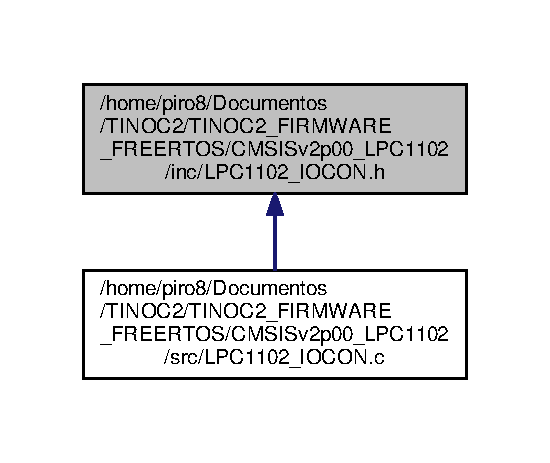
\includegraphics[width=264pt]{_l_p_c1102___i_o_c_o_n_8h__dep__incl}
\end{center}
\end{figure}
\subsection*{Macros}
\begin{DoxyCompactItemize}
\item 
\#define \hyperlink{group___l_p_c___i_o_c_o_n___l_p_c1102___b_i_t_s_ga2d9600555b95756df39218dbb47851ae}{L\+P\+C\+\_\+\+I\+O\+C\+O\+N\+\_\+\+F\+U\+N\+C\+\_\+\+B\+IT}~(0)
\begin{DoxyCompactList}\small\item\em Bit de función. \end{DoxyCompactList}\item 
\#define \hyperlink{group___l_p_c___i_o_c_o_n___l_p_c1102___b_i_t_s_ga793b5ab5e1ab4f784e43a86a2d1ff21f}{L\+P\+C\+\_\+\+I\+O\+C\+O\+N\+\_\+\+M\+O\+D\+E\+\_\+\+B\+IT}~(3)
\begin{DoxyCompactList}\small\item\em Bits de Modo. \end{DoxyCompactList}\item 
\#define \hyperlink{group___l_p_c___i_o_c_o_n___l_p_c1102___b_i_t_s_ga4bdb40fca164c65756bd1c3e69207b62}{L\+P\+C\+\_\+\+I\+O\+C\+O\+N\+\_\+\+H\+Y\+S\+\_\+\+B\+IT}~(5)
\begin{DoxyCompactList}\small\item\em Bit de histeresis. \end{DoxyCompactList}\item 
\#define \hyperlink{group___l_p_c___i_o_c_o_n___l_p_c1102___b_i_t_s_ga0ed826952d05716fdcf3252675de3b93}{L\+P\+C\+\_\+\+I\+O\+C\+O\+N\+\_\+\+A\+D\+M\+O\+D\+E\+\_\+\+B\+IT}~(7)
\begin{DoxyCompactList}\small\item\em Bit de modo analogico o digital. \end{DoxyCompactList}\item 
\#define \hyperlink{group___l_p_c___i_o_c_o_n___l_p_c1102___b_i_t_s_ga62a2b807caf0cfa8371cf1df6f5c9a21}{L\+P\+C\+\_\+\+I\+O\+C\+O\+N\+\_\+\+O\+D\+\_\+\+B\+IT}~(10)
\begin{DoxyCompactList}\small\item\em Bit de Open Drain. \end{DoxyCompactList}\item 
\#define \hyperlink{group___l_p_c___i_o_c_o_n___l_p_c1102___m_a_s_c_a_r_a_s_ga429d63df506589f85224d3c12fd61e3b}{L\+P\+C\+\_\+\+I\+O\+C\+O\+N\+\_\+\+F\+U\+N\+C\+\_\+\+M\+AS}~(0x00000007\+U\+L) $<$$<$ L\+P\+C\+\_\+\+I\+O\+C\+O\+N\+\_\+\+F\+U\+N\+C\+\_\+\+B\+IT
\item 
\#define \hyperlink{group___l_p_c___i_o_c_o_n___l_p_c1102___m_a_s_c_a_r_a_s_gac56363757324c51a61e36e9471024b05}{L\+P\+C\+\_\+\+I\+O\+C\+O\+N\+\_\+\+M\+O\+D\+E\+\_\+\+M\+AS}~(0x00000003\+U\+L) $<$$<$ L\+P\+C\+\_\+\+I\+O\+C\+O\+N\+\_\+\+M\+O\+D\+E\+\_\+\+B\+IT
\item 
\#define \hyperlink{group___l_p_c___i_o_c_o_n___l_p_c1102___m_a_s_c_a_r_a_s_ga0f8ccfc34bf41c0deced30305a2d17e5}{L\+P\+C\+\_\+\+I\+O\+C\+O\+N\+\_\+\+H\+Y\+S\+\_\+\+M\+AS}~(0x00000001\+U\+L) $<$$<$ L\+P\+C\+\_\+\+I\+O\+C\+O\+N\+\_\+\+H\+Y\+S\+\_\+\+B\+IT
\item 
\#define \hyperlink{group___l_p_c___i_o_c_o_n___l_p_c1102___m_a_s_c_a_r_a_s_ga63379280f01e70a858b26114f4949794}{L\+P\+C\+\_\+\+I\+O\+C\+O\+N\+\_\+\+O\+D\+\_\+\+M\+AS}~(0x00000001\+U\+L) $<$$<$ L\+P\+C\+\_\+\+I\+O\+C\+O\+N\+\_\+\+O\+D\+\_\+\+B\+IT
\item 
\#define \hyperlink{group___l_p_c___i_o_c_o_n___l_p_c1102___m_o_d_e_gac0cfc0275160b96c647fc5774f34b390}{L\+P\+C\+\_\+\+I\+O\+C\+O\+N\+\_\+\+M\+O\+D\+E\+\_\+\+I\+N\+A\+C\+T\+I\+VE}~(0x00000000\+U\+L) $<$$<$ L\+P\+C\+\_\+\+I\+O\+C\+O\+N\+\_\+\+M\+O\+D\+E\+\_\+\+B\+IT
\begin{DoxyCompactList}\small\item\em Inactivo \+: sin resistencia pull-\/down/pull-\/up. \end{DoxyCompactList}\item 
\#define \hyperlink{group___l_p_c___i_o_c_o_n___l_p_c1102___m_o_d_e_gac740c9895b3d9f1c49a902a7693b3ef4}{L\+P\+C\+\_\+\+I\+O\+C\+O\+N\+\_\+\+M\+O\+D\+E\+\_\+\+P\+U\+L\+L\+D\+O\+WN}~(0x00000001\+U\+L) $<$$<$ L\+P\+C\+\_\+\+I\+O\+C\+O\+N\+\_\+\+M\+O\+D\+E\+\_\+\+B\+IT
\begin{DoxyCompactList}\small\item\em Resistencia de Pull-\/\+Down habilitada. \end{DoxyCompactList}\item 
\#define \hyperlink{group___l_p_c___i_o_c_o_n___l_p_c1102___m_o_d_e_ga36c30fc68af8e4dfdda3ed4116bbb9e1}{L\+P\+C\+\_\+\+I\+O\+C\+O\+N\+\_\+\+M\+O\+D\+E\+\_\+\+P\+U\+L\+L\+UP}~(0x00000002\+U\+L) $<$$<$ L\+P\+C\+\_\+\+I\+O\+C\+O\+N\+\_\+\+M\+O\+D\+E\+\_\+\+B\+IT
\begin{DoxyCompactList}\small\item\em Resistencia de Pull-\/\+Up habilitada. \end{DoxyCompactList}\item 
\#define \hyperlink{group___l_p_c___i_o_c_o_n___l_p_c1102___m_o_d_e_ga622cda7f7867ff277096fe6ccb94d046}{L\+P\+C\+\_\+\+I\+O\+C\+O\+N\+\_\+\+M\+O\+D\+E\+\_\+\+R\+E\+P\+E\+A\+T\+ER}~(0x00000003\+U\+L) $<$$<$ L\+P\+C\+\_\+\+I\+O\+C\+O\+N\+\_\+\+M\+O\+D\+E\+\_\+\+B\+IT
\begin{DoxyCompactList}\small\item\em Modo repetidor. \end{DoxyCompactList}\item 
\#define \hyperlink{group___l_p_c___i_o_c_o_n___l_p_c1102___a_s_o_c_i_a_c_i_o_n_e_s_gadf840fda55b54a90ad1ae46d4f2abe29}{L\+P\+C\+\_\+\+I\+O\+C\+O\+N\+\_\+\+C1}~\hyperlink{group___l_p_c11xx___definitions_gaabc651799ba17b0dd4a0114c8d48a145}{L\+P\+C\+\_\+\+I\+O\+C\+ON}-\/$>$R\+E\+S\+E\+T\+\_\+\+P\+I\+O0\+\_\+0
\item 
\#define \hyperlink{group___l_p_c___i_o_c_o_n___l_p_c1102___a_s_o_c_i_a_c_i_o_n_e_s_gad07b47c89c86b1b5688e116e09357df6}{L\+P\+C\+\_\+\+I\+O\+C\+O\+N\+\_\+\+A2}~\hyperlink{group___l_p_c11xx___definitions_gaabc651799ba17b0dd4a0114c8d48a145}{L\+P\+C\+\_\+\+I\+O\+C\+ON}-\/$>$P\+I\+O0\+\_\+8
\item 
\#define \hyperlink{group___l_p_c___i_o_c_o_n___l_p_c1102___a_s_o_c_i_a_c_i_o_n_e_s_ga30b8aa33fff57304e533c0a5f5a80d9a}{L\+P\+C\+\_\+\+I\+O\+C\+O\+N\+\_\+\+A3}~\hyperlink{group___l_p_c11xx___definitions_gaabc651799ba17b0dd4a0114c8d48a145}{L\+P\+C\+\_\+\+I\+O\+C\+ON}-\/$>$P\+I\+O0\+\_\+9
\item 
\#define \hyperlink{group___l_p_c___i_o_c_o_n___l_p_c1102___a_s_o_c_i_a_c_i_o_n_e_s_ga58fdb2acc1fb471de0c2e6579996c501}{L\+P\+C\+\_\+\+I\+O\+C\+O\+N\+\_\+\+A4}~\hyperlink{group___l_p_c11xx___definitions_gaabc651799ba17b0dd4a0114c8d48a145}{L\+P\+C\+\_\+\+I\+O\+C\+ON}-\/$>$S\+W\+C\+L\+K\+\_\+\+P\+I\+O0\+\_\+10
\item 
\#define \hyperlink{group___l_p_c___i_o_c_o_n___l_p_c1102___a_s_o_c_i_a_c_i_o_n_e_s_ga4a57e0dbac00d893c3aba917a8295e2d}{L\+P\+C\+\_\+\+I\+O\+C\+O\+N\+\_\+\+B4}~\hyperlink{group___l_p_c11xx___definitions_gaabc651799ba17b0dd4a0114c8d48a145}{L\+P\+C\+\_\+\+I\+O\+C\+ON}-\/$>$R\+\_\+\+P\+I\+O0\+\_\+11
\item 
\#define \hyperlink{group___l_p_c___i_o_c_o_n___l_p_c1102___a_s_o_c_i_a_c_i_o_n_e_s_gaabdb13248922a7b2c88b212a48d943b9}{L\+P\+C\+\_\+\+I\+O\+C\+O\+N\+\_\+\+B3}~\hyperlink{group___l_p_c11xx___definitions_gaabc651799ba17b0dd4a0114c8d48a145}{L\+P\+C\+\_\+\+I\+O\+C\+ON}-\/$>$R\+\_\+\+P\+I\+O1\+\_\+0
\item 
\#define \hyperlink{group___l_p_c___i_o_c_o_n___l_p_c1102___a_s_o_c_i_a_c_i_o_n_e_s_ga434a8f458a9a2656343d24444391f2c8}{L\+P\+C\+\_\+\+I\+O\+C\+O\+N\+\_\+\+C4}~\hyperlink{group___l_p_c11xx___definitions_gaabc651799ba17b0dd4a0114c8d48a145}{L\+P\+C\+\_\+\+I\+O\+C\+ON}-\/$>$R\+\_\+\+P\+I\+O1\+\_\+1
\item 
\#define \hyperlink{group___l_p_c___i_o_c_o_n___l_p_c1102___a_s_o_c_i_a_c_i_o_n_e_s_ga285291cb7f4f7bae6c08f7a6ca2885a2}{L\+P\+C\+\_\+\+I\+O\+C\+O\+N\+\_\+\+C3}~\hyperlink{group___l_p_c11xx___definitions_gaabc651799ba17b0dd4a0114c8d48a145}{L\+P\+C\+\_\+\+I\+O\+C\+ON}-\/$>$R\+\_\+\+P\+I\+O1\+\_\+2
\item 
\#define \hyperlink{group___l_p_c___i_o_c_o_n___l_p_c1102___a_s_o_c_i_a_c_i_o_n_e_s_ga25bed3139a10eb803a6e2e017fa255f9}{L\+P\+C\+\_\+\+I\+O\+C\+O\+N\+\_\+\+D4}~\hyperlink{group___l_p_c11xx___definitions_gaabc651799ba17b0dd4a0114c8d48a145}{L\+P\+C\+\_\+\+I\+O\+C\+ON}-\/$>$S\+W\+D\+I\+O\+\_\+\+P\+I\+O1\+\_\+3
\item 
\#define \hyperlink{group___l_p_c___i_o_c_o_n___l_p_c1102___a_s_o_c_i_a_c_i_o_n_e_s_ga73459d08b19f5790fa4f7514108d515b}{L\+P\+C\+\_\+\+I\+O\+C\+O\+N\+\_\+\+C2}~\hyperlink{group___l_p_c11xx___definitions_gaabc651799ba17b0dd4a0114c8d48a145}{L\+P\+C\+\_\+\+I\+O\+C\+ON}-\/$>$P\+I\+O1\+\_\+6
\item 
\#define \hyperlink{group___l_p_c___i_o_c_o_n___l_p_c1102___a_s_o_c_i_a_c_i_o_n_e_s_gae3021c481ea6e4bf372e5cd17e118f37}{L\+P\+C\+\_\+\+I\+O\+C\+O\+N\+\_\+\+D1}~\hyperlink{group___l_p_c11xx___definitions_gaabc651799ba17b0dd4a0114c8d48a145}{L\+P\+C\+\_\+\+I\+O\+C\+ON}-\/$>$P\+I\+O1\+\_\+7
\item 
\#define \hyperlink{group___l_p_c___i_o_c_o_n___l_p_c1102___s_c_k___l_o_c_ga831c058cf3b0a147b5833bfac8ddce82}{L\+P\+C\+\_\+\+I\+O\+C\+O\+N\+\_\+\+S\+C\+K\+L\+O\+C\+\_\+\+B\+IT}~(0)
\begin{DoxyCompactList}\small\item\em Bit del registro para modificar el pin S\+C\+K\+L\+OC. \end{DoxyCompactList}\item 
\#define \hyperlink{group___l_p_c___i_o_c_o_n___l_p_c1102___s_c_k___l_o_c_gaba2d4230db5fd5477c8f1bd850d90963}{L\+P\+C\+\_\+\+I\+O\+C\+O\+N\+\_\+\+S\+C\+K\+L\+O\+C\+\_\+\+P0\+\_\+10}~(0x00000000\+U\+L) $<$$<$ L\+P\+C\+\_\+\+I\+O\+C\+O\+N\+\_\+\+S\+C\+K\+L\+O\+C\+\_\+\+B\+IT
\begin{DoxyCompactList}\small\item\em Asocio la función de S\+CK al Pin P0.\+10 A4 (por default en L\+P\+C1102) \end{DoxyCompactList}\item 
\#define \hyperlink{group___l_p_c___i_o_c_o_n___l_p_c1102___s_c_k___l_o_c_gaa6d2e11946beb81a3e4260e789fe67fe}{L\+P\+C\+\_\+\+I\+O\+C\+O\+N\+\_\+\+S\+C\+K\+L\+O\+C\+\_\+\+P0\+\_\+6}~(0x00000002\+U\+L) $<$$<$ L\+P\+C\+\_\+\+I\+O\+C\+O\+N\+\_\+\+S\+C\+K\+L\+O\+C\+\_\+\+B\+IT
\begin{DoxyCompactList}\small\item\em Asocio la función de S\+CK al Pin P0.\+6 A1 solo en L\+P\+C1104. \end{DoxyCompactList}\item 
\#define \hyperlink{_l_p_c1102___i_o_c_o_n_8h_a6f355bec112f7153727de6d58cf3c685}{D\+E\+F\+I\+N\+I\+R\+\_\+\+P\+I\+N\+\_\+\+C\+O\+N\+F\+I\+G\+U\+R\+A\+C\+I\+O\+N\+\_\+\+I\+O\+\_\+\+E\+R\+R\+O\+R\+\_\+\+P\+IN}~1
\end{DoxyCompactItemize}
\begin{Indent}{\bf C1 -\/ R\+E\+S\+E\+T/\+P0.0}\par
\begin{DoxyCompactItemize}
\item 
\#define \hyperlink{group___l_p_c___i_o_c_o_n___l_p_c1102___p_i_n_e_s_gac743a21ae6fb018103e15efe2ea9487e}{L\+P\+C\+\_\+\+I\+O\+C\+O\+N\+\_\+\+C1\+\_\+\+F\+U\+N\+C\+\_\+\+R\+E\+S\+ET}~(0x00000000\+U\+L) $<$$<$ L\+P\+C\+\_\+\+I\+O\+C\+O\+N\+\_\+\+F\+U\+N\+C\+\_\+\+B\+IT
\item 
\#define \hyperlink{group___l_p_c___i_o_c_o_n___l_p_c1102___p_i_n_e_s_gafade20b5f097f138815526a37ea5b86e}{L\+P\+C\+\_\+\+I\+O\+C\+O\+N\+\_\+\+C1\+\_\+\+F\+U\+N\+C\+\_\+\+P\+I\+O0\+\_\+0}~(0x00000001\+U\+L) $<$$<$ L\+P\+C\+\_\+\+I\+O\+C\+O\+N\+\_\+\+F\+U\+N\+C\+\_\+\+B\+IT
\end{DoxyCompactItemize}
\end{Indent}
\begin{Indent}{\bf A2 -\/ P0.8/\+M\+I\+S\+O/\+C\+T16\+B0\+\_\+\+M\+A\+T0}\par
\begin{DoxyCompactItemize}
\item 
\#define \hyperlink{group___l_p_c___i_o_c_o_n___l_p_c1102___p_i_n_e_s_ga73249c352adc2c4eb07089edf856904e}{L\+P\+C\+\_\+\+I\+O\+C\+O\+N\+\_\+\+A2\+\_\+\+F\+U\+N\+C\+\_\+\+P\+I\+O0\+\_\+8}~(0x00000000\+U\+L) $<$$<$ L\+P\+C\+\_\+\+I\+O\+C\+O\+N\+\_\+\+F\+U\+N\+C\+\_\+\+B\+IT
\item 
\#define \hyperlink{group___l_p_c___i_o_c_o_n___l_p_c1102___p_i_n_e_s_gac2cf122fa3f708da105cdeba5c33215c}{L\+P\+C\+\_\+\+I\+O\+C\+O\+N\+\_\+\+A2\+\_\+\+F\+U\+N\+C\+\_\+\+M\+I\+S\+O0}~(0x00000001\+U\+L) $<$$<$ L\+P\+C\+\_\+\+I\+O\+C\+O\+N\+\_\+\+F\+U\+N\+C\+\_\+\+B\+IT
\item 
\#define \hyperlink{group___l_p_c___i_o_c_o_n___l_p_c1102___p_i_n_e_s_gae8b3d16d47cc34abc8668f6e5a9ef62b}{L\+P\+C\+\_\+\+I\+O\+C\+O\+N\+\_\+\+A2\+\_\+\+F\+U\+N\+C\+\_\+\+C\+T16\+B0\+\_\+\+M\+A\+T0}~(0x00000002\+U\+L) $<$$<$ L\+P\+C\+\_\+\+I\+O\+C\+O\+N\+\_\+\+F\+U\+N\+C\+\_\+\+B\+IT
\end{DoxyCompactItemize}
\end{Indent}
\begin{Indent}{\bf A3 -\/ P0.9/\+M\+O\+S\+I/\+C\+T16\+B0\+\_\+\+M\+A\+T1}\par
\begin{DoxyCompactItemize}
\item 
\#define \hyperlink{group___l_p_c___i_o_c_o_n___l_p_c1102___p_i_n_e_s_gab2f89db29fd04f6a1d1c3111cd3da9f2}{L\+P\+C\+\_\+\+I\+O\+C\+O\+N\+\_\+\+A3\+\_\+\+F\+U\+N\+C\+\_\+\+P\+I\+O0\+\_\+9}~(0x00000000\+U\+L) $<$$<$ L\+P\+C\+\_\+\+I\+O\+C\+O\+N\+\_\+\+F\+U\+N\+C\+\_\+\+B\+IT
\item 
\#define \hyperlink{group___l_p_c___i_o_c_o_n___l_p_c1102___p_i_n_e_s_ga75592faa0d4e235173f790ee80e79651}{L\+P\+C\+\_\+\+I\+O\+C\+O\+N\+\_\+\+A3\+\_\+\+F\+U\+N\+C\+\_\+\+M\+O\+S\+I0}~(0x00000001\+U\+L) $<$$<$ L\+P\+C\+\_\+\+I\+O\+C\+O\+N\+\_\+\+F\+U\+N\+C\+\_\+\+B\+IT
\item 
\#define \hyperlink{group___l_p_c___i_o_c_o_n___l_p_c1102___p_i_n_e_s_gab8c36d6638e434a9db7d3e43e4a5e768}{L\+P\+C\+\_\+\+I\+O\+C\+O\+N\+\_\+\+A3\+\_\+\+F\+U\+N\+C\+\_\+\+C\+T16\+B0\+\_\+\+M\+A\+T1}~(0x00000002\+U\+L) $<$$<$ L\+P\+C\+\_\+\+I\+O\+C\+O\+N\+\_\+\+F\+U\+N\+C\+\_\+\+B\+IT
\end{DoxyCompactItemize}
\end{Indent}
\begin{Indent}{\bf A4 -\/ S\+W\+C\+L\+K/\+P0.10/\+S\+C\+K0/\+C\+T16\+B0\+\_\+\+M\+A\+T2}\par
\begin{DoxyCompactItemize}
\item 
\#define \hyperlink{group___l_p_c___i_o_c_o_n___l_p_c1102___p_i_n_e_s_ga71ead8726fc622434f9b4222c5778f60}{L\+P\+C\+\_\+\+I\+O\+C\+O\+N\+\_\+\+A4\+\_\+\+F\+U\+N\+C\+\_\+\+S\+W\+C\+LK}~(0x00000000\+U\+L) $<$$<$ L\+P\+C\+\_\+\+I\+O\+C\+O\+N\+\_\+\+F\+U\+N\+C\+\_\+\+B\+IT
\item 
\#define \hyperlink{group___l_p_c___i_o_c_o_n___l_p_c1102___p_i_n_e_s_ga87cbf13f8963feae2c0ed0efa8207443}{L\+P\+C\+\_\+\+I\+O\+C\+O\+N\+\_\+\+A4\+\_\+\+F\+U\+N\+C\+\_\+\+P\+I\+O0\+\_\+10}~(0x00000001\+U\+L) $<$$<$ L\+P\+C\+\_\+\+I\+O\+C\+O\+N\+\_\+\+F\+U\+N\+C\+\_\+\+B\+IT
\item 
\#define \hyperlink{group___l_p_c___i_o_c_o_n___l_p_c1102___p_i_n_e_s_ga15f501e83044f160bad331f583ff0de2}{L\+P\+C\+\_\+\+I\+O\+C\+O\+N\+\_\+\+A4\+\_\+\+F\+U\+N\+C\+\_\+\+S\+C\+K0}~(0x00000002\+U\+L) $<$$<$ L\+P\+C\+\_\+\+I\+O\+C\+O\+N\+\_\+\+F\+U\+N\+C\+\_\+\+B\+IT
\item 
\#define \hyperlink{group___l_p_c___i_o_c_o_n___l_p_c1102___p_i_n_e_s_ga1d8317d7eab94b27acec3dd6566e1603}{L\+P\+C\+\_\+\+I\+O\+C\+O\+N\+\_\+\+A4\+\_\+\+F\+U\+N\+C\+\_\+\+C\+T16\+B0\+\_\+\+M\+A\+T2}~(0x00000003\+U\+L) $<$$<$ L\+P\+C\+\_\+\+I\+O\+C\+O\+N\+\_\+\+F\+U\+N\+C\+\_\+\+B\+IT
\end{DoxyCompactItemize}
\end{Indent}
\begin{Indent}{\bf B4 -\/ R/\+P0.11/\+A\+D0/\+C\+T32\+B0\+\_\+\+M\+A\+T3}\par
\begin{DoxyCompactItemize}
\item 
\#define \hyperlink{group___l_p_c___i_o_c_o_n___l_p_c1102___p_i_n_e_s_gaaf9bca59195d557afe0706795adde87b}{L\+P\+C\+\_\+\+I\+O\+C\+O\+N\+\_\+\+B4\+\_\+\+F\+U\+N\+C\+\_\+R}~(0x00000000\+U\+L) $<$$<$ L\+P\+C\+\_\+\+I\+O\+C\+O\+N\+\_\+\+F\+U\+N\+C\+\_\+\+B\+IT
\item 
\#define \hyperlink{group___l_p_c___i_o_c_o_n___l_p_c1102___p_i_n_e_s_ga772b2ba88b3dbd3457e63a5e41a52a05}{L\+P\+C\+\_\+\+I\+O\+C\+O\+N\+\_\+\+B4\+\_\+\+F\+U\+N\+C\+\_\+\+P\+I\+O0\+\_\+11}~(0x00000001\+U\+L) $<$$<$ L\+P\+C\+\_\+\+I\+O\+C\+O\+N\+\_\+\+F\+U\+N\+C\+\_\+\+B\+IT
\item 
\#define \hyperlink{group___l_p_c___i_o_c_o_n___l_p_c1102___p_i_n_e_s_gae81155dea1ee849ae1324fbe36b9ebb7}{L\+P\+C\+\_\+\+I\+O\+C\+O\+N\+\_\+\+B4\+\_\+\+F\+U\+N\+C\+\_\+\+A\+D0}~(0x00000002\+U\+L) $<$$<$ L\+P\+C\+\_\+\+I\+O\+C\+O\+N\+\_\+\+F\+U\+N\+C\+\_\+\+B\+IT
\item 
\#define \hyperlink{group___l_p_c___i_o_c_o_n___l_p_c1102___p_i_n_e_s_gaf233dc12f01fa1193a2c8916c7b62960}{L\+P\+C\+\_\+\+I\+O\+C\+O\+N\+\_\+\+B4\+\_\+\+F\+U\+N\+C\+\_\+\+C\+T16\+B0\+\_\+\+M\+A\+T3}~(0x00000003\+U\+L) $<$$<$ L\+P\+C\+\_\+\+I\+O\+C\+O\+N\+\_\+\+F\+U\+N\+C\+\_\+\+B\+IT
\end{DoxyCompactItemize}
\end{Indent}
\begin{Indent}{\bf B3 -\/ R/\+P1.0/\+A\+D1/\+C\+T32\+B1\+\_\+\+C\+A\+P0}\par
\begin{DoxyCompactItemize}
\item 
\#define \hyperlink{group___l_p_c___i_o_c_o_n___l_p_c1102___p_i_n_e_s_ga745545f76e10bc8663d8abf205ce3417}{L\+P\+C\+\_\+\+I\+O\+C\+O\+N\+\_\+\+B3\+\_\+\+F\+U\+N\+C\+\_\+R}~(0x00000000\+U\+L) $<$$<$ L\+P\+C\+\_\+\+I\+O\+C\+O\+N\+\_\+\+F\+U\+N\+C\+\_\+\+B\+IT
\item 
\#define \hyperlink{group___l_p_c___i_o_c_o_n___l_p_c1102___p_i_n_e_s_ga05526127ae3fdce2a8b9d838e7c0f6d0}{L\+P\+C\+\_\+\+I\+O\+C\+O\+N\+\_\+\+B3\+\_\+\+F\+U\+N\+C\+\_\+\+P\+I\+O1\+\_\+0}~(0x00000001\+U\+L) $<$$<$ L\+P\+C\+\_\+\+I\+O\+C\+O\+N\+\_\+\+F\+U\+N\+C\+\_\+\+B\+IT
\item 
\#define \hyperlink{group___l_p_c___i_o_c_o_n___l_p_c1102___p_i_n_e_s_gaf638fc4d9aea6f2b8f9b5bf1ab0f6942}{L\+P\+C\+\_\+\+I\+O\+C\+O\+N\+\_\+\+B3\+\_\+\+F\+U\+N\+C\+\_\+\+A\+D1}~(0x00000002\+U\+L) $<$$<$ L\+P\+C\+\_\+\+I\+O\+C\+O\+N\+\_\+\+F\+U\+N\+C\+\_\+\+B\+IT
\item 
\#define \hyperlink{group___l_p_c___i_o_c_o_n___l_p_c1102___p_i_n_e_s_gad92721a2f17acdc507bde9b386b6517a}{L\+P\+C\+\_\+\+I\+O\+C\+O\+N\+\_\+\+B3\+\_\+\+F\+U\+N\+C\+\_\+\+C\+T32\+B1\+\_\+\+C\+A\+P0}~(0x00000003\+U\+L) $<$$<$ L\+P\+C\+\_\+\+I\+O\+C\+O\+N\+\_\+\+F\+U\+N\+C\+\_\+\+B\+IT
\end{DoxyCompactItemize}
\end{Indent}
\begin{Indent}{\bf C4 -\/ R/\+P1.1/\+A\+D2/\+C\+T32\+B1\+\_\+\+M\+A\+T0}\par
\begin{DoxyCompactItemize}
\item 
\#define \hyperlink{group___l_p_c___i_o_c_o_n___l_p_c1102___p_i_n_e_s_ga5109d5a6418fa651ad73bc316a2ca64d}{L\+P\+C\+\_\+\+I\+O\+C\+O\+N\+\_\+\+C4\+\_\+\+F\+U\+N\+C\+\_\+R}~(0x00000000\+U\+L) $<$$<$ L\+P\+C\+\_\+\+I\+O\+C\+O\+N\+\_\+\+F\+U\+N\+C\+\_\+\+B\+IT
\item 
\#define \hyperlink{group___l_p_c___i_o_c_o_n___l_p_c1102___p_i_n_e_s_ga68ee6b56ec7c4eea69bb4602a44f2bf3}{L\+P\+C\+\_\+\+I\+O\+C\+O\+N\+\_\+\+C4\+\_\+\+F\+U\+N\+C\+\_\+\+P\+I\+O1\+\_\+1}~(0x00000001\+U\+L) $<$$<$ L\+P\+C\+\_\+\+I\+O\+C\+O\+N\+\_\+\+F\+U\+N\+C\+\_\+\+B\+IT
\item 
\#define \hyperlink{group___l_p_c___i_o_c_o_n___l_p_c1102___p_i_n_e_s_gad03ecd173dbeb860f3ef155bf598debc}{L\+P\+C\+\_\+\+I\+O\+C\+O\+N\+\_\+\+C4\+\_\+\+F\+U\+N\+C\+\_\+\+A\+D2}~(0x00000002\+U\+L) $<$$<$ L\+P\+C\+\_\+\+I\+O\+C\+O\+N\+\_\+\+F\+U\+N\+C\+\_\+\+B\+IT
\item 
\#define \hyperlink{group___l_p_c___i_o_c_o_n___l_p_c1102___p_i_n_e_s_gad9da73ec7045034730c0ac2540a34c16}{L\+P\+C\+\_\+\+I\+O\+C\+O\+N\+\_\+\+C4\+\_\+\+F\+U\+N\+C\+\_\+\+C\+T32\+B1\+\_\+\+M\+A\+T0}~(0x00000003\+U\+L) $<$$<$ L\+P\+C\+\_\+\+I\+O\+C\+O\+N\+\_\+\+F\+U\+N\+C\+\_\+\+B\+IT
\end{DoxyCompactItemize}
\end{Indent}
\begin{Indent}{\bf C3 -\/ R/\+P1.2/\+A\+D3/\+C\+T32\+B1\+\_\+\+M\+A\+T1}\par
\begin{DoxyCompactItemize}
\item 
\#define \hyperlink{group___l_p_c___i_o_c_o_n___l_p_c1102___p_i_n_e_s_ga0ce0c613a070b5c4df0d5cc9ceda8295}{L\+P\+C\+\_\+\+I\+O\+C\+O\+N\+\_\+\+C3\+\_\+\+F\+U\+N\+C\+\_\+R}~(0x00000000\+U\+L) $<$$<$ L\+P\+C\+\_\+\+I\+O\+C\+O\+N\+\_\+\+F\+U\+N\+C\+\_\+\+B\+IT
\item 
\#define \hyperlink{group___l_p_c___i_o_c_o_n___l_p_c1102___p_i_n_e_s_ga0a8c9225a9d80bf16239e67d7e321bf3}{L\+P\+C\+\_\+\+I\+O\+C\+O\+N\+\_\+\+C3\+\_\+\+F\+U\+N\+C\+\_\+\+P\+I\+O1\+\_\+2}~(0x00000001\+U\+L) $<$$<$ L\+P\+C\+\_\+\+I\+O\+C\+O\+N\+\_\+\+F\+U\+N\+C\+\_\+\+B\+IT
\item 
\#define \hyperlink{group___l_p_c___i_o_c_o_n___l_p_c1102___p_i_n_e_s_ga3ba9a8b0b1234e4b1d8d8f2ebf5cbec6}{L\+P\+C\+\_\+\+I\+O\+C\+O\+N\+\_\+\+C3\+\_\+\+F\+U\+N\+C\+\_\+\+A\+D3}~(0x00000002\+U\+L) $<$$<$ L\+P\+C\+\_\+\+I\+O\+C\+O\+N\+\_\+\+F\+U\+N\+C\+\_\+\+B\+IT
\item 
\#define \hyperlink{group___l_p_c___i_o_c_o_n___l_p_c1102___p_i_n_e_s_gafb52d80ad556237649f92c38416825d3}{L\+P\+C\+\_\+\+I\+O\+C\+O\+N\+\_\+\+C3\+\_\+\+F\+U\+N\+C\+\_\+\+C\+T32\+B1\+\_\+\+M\+A\+T1}~(0x00000003\+U\+L) $<$$<$ L\+P\+C\+\_\+\+I\+O\+C\+O\+N\+\_\+\+F\+U\+N\+C\+\_\+\+B\+IT
\end{DoxyCompactItemize}
\end{Indent}
\begin{Indent}{\bf D4 -\/ S\+W\+D\+I\+O/\+P1.3/\+A\+D4/\+C\+T32\+B1\+\_\+\+M\+A\+T2}\par
\begin{DoxyCompactItemize}
\item 
\#define \hyperlink{group___l_p_c___i_o_c_o_n___l_p_c1102___p_i_n_e_s_ga7d0843dbf1f39f41e01cdcf0ea1396f8}{L\+P\+C\+\_\+\+I\+O\+C\+O\+N\+\_\+\+D4\+\_\+\+F\+U\+N\+C\+\_\+\+S\+W\+D\+IO}~(0x00000000\+U\+L) $<$$<$ L\+P\+C\+\_\+\+I\+O\+C\+O\+N\+\_\+\+F\+U\+N\+C\+\_\+\+B\+IT
\item 
\#define \hyperlink{group___l_p_c___i_o_c_o_n___l_p_c1102___p_i_n_e_s_ga029a20695f231fa2f81d7bd0642a6f85}{L\+P\+C\+\_\+\+I\+O\+C\+O\+N\+\_\+\+D4\+\_\+\+F\+U\+N\+C\+\_\+\+P\+I\+O1\+\_\+3}~(0x00000001\+U\+L) $<$$<$ L\+P\+C\+\_\+\+I\+O\+C\+O\+N\+\_\+\+F\+U\+N\+C\+\_\+\+B\+IT
\item 
\#define \hyperlink{group___l_p_c___i_o_c_o_n___l_p_c1102___p_i_n_e_s_ga73cef70ce7760ccd240ddf0b26a33656}{L\+P\+C\+\_\+\+I\+O\+C\+O\+N\+\_\+\+D4\+\_\+\+F\+U\+N\+C\+\_\+\+A\+D4}~(0x00000002\+U\+L) $<$$<$ L\+P\+C\+\_\+\+I\+O\+C\+O\+N\+\_\+\+F\+U\+N\+C\+\_\+\+B\+IT
\item 
\#define \hyperlink{group___l_p_c___i_o_c_o_n___l_p_c1102___p_i_n_e_s_ga07986c77c1b43eb5994da559abfda911}{L\+P\+C\+\_\+\+I\+O\+C\+O\+N\+\_\+\+D4\+\_\+\+F\+U\+N\+C\+\_\+\+C\+T32\+B1\+\_\+\+M\+A\+T2}~(0x00000003\+U\+L) $<$$<$ L\+P\+C\+\_\+\+I\+O\+C\+O\+N\+\_\+\+F\+U\+N\+C\+\_\+\+B\+IT
\end{DoxyCompactItemize}
\end{Indent}
\begin{Indent}{\bf C2 -\/ P1.6/\+R\+X\+D/\+C\+T32\+B0\+\_\+\+M\+A\+T0}\par
\begin{DoxyCompactItemize}
\item 
\#define \hyperlink{group___l_p_c___i_o_c_o_n___l_p_c1102___p_i_n_e_s_ga0f09acebc3f44b34a3b2a42a13888bd4}{L\+P\+C\+\_\+\+I\+O\+C\+O\+N\+\_\+\+C2\+\_\+\+F\+U\+N\+C\+\_\+\+P\+I\+O1\+\_\+3}~(0x00000000\+U\+L) $<$$<$ L\+P\+C\+\_\+\+I\+O\+C\+O\+N\+\_\+\+F\+U\+N\+C\+\_\+\+B\+IT
\item 
\#define \hyperlink{group___l_p_c___i_o_c_o_n___l_p_c1102___p_i_n_e_s_ga2d578e6a171300d7662cbc772e561709}{L\+P\+C\+\_\+\+I\+O\+C\+O\+N\+\_\+\+C2\+\_\+\+F\+U\+N\+C\+\_\+\+R\+XD}~(0x00000001\+U\+L) $<$$<$ L\+P\+C\+\_\+\+I\+O\+C\+O\+N\+\_\+\+F\+U\+N\+C\+\_\+\+B\+IT
\item 
\#define \hyperlink{group___l_p_c___i_o_c_o_n___l_p_c1102___p_i_n_e_s_ga747cbcdca6a691c32f20216f8d25b0c1}{L\+P\+C\+\_\+\+I\+O\+C\+O\+N\+\_\+\+C4\+\_\+\+F\+U\+N\+C\+\_\+\+C\+T32\+B0\+\_\+\+M\+A\+T0}~(0x00000002\+U\+L) $<$$<$ L\+P\+C\+\_\+\+I\+O\+C\+O\+N\+\_\+\+F\+U\+N\+C\+\_\+\+B\+IT
\end{DoxyCompactItemize}
\end{Indent}
\begin{Indent}{\bf D1 -\/ P1.7/\+T\+X\+D/\+C\+T32\+B0\+\_\+\+M\+A\+T1}\par
\begin{DoxyCompactItemize}
\item 
\#define \hyperlink{group___l_p_c___i_o_c_o_n___l_p_c1102___p_i_n_e_s_gaffb3310b8c854e58d1f5e3c2449df182}{L\+P\+C\+\_\+\+I\+O\+C\+O\+N\+\_\+\+D1\+\_\+\+F\+U\+N\+C\+\_\+\+P\+I\+O1\+\_\+7}~(0x00000000\+U\+L) $<$$<$ L\+P\+C\+\_\+\+I\+O\+C\+O\+N\+\_\+\+F\+U\+N\+C\+\_\+\+B\+IT
\item 
\#define \hyperlink{group___l_p_c___i_o_c_o_n___l_p_c1102___p_i_n_e_s_ga20f8d9546ce4f038a1546f542241ba86}{L\+P\+C\+\_\+\+I\+O\+C\+O\+N\+\_\+\+D1\+\_\+\+F\+U\+N\+C\+\_\+\+T\+XD}~(0x00000001\+U\+L) $<$$<$ L\+P\+C\+\_\+\+I\+O\+C\+O\+N\+\_\+\+F\+U\+N\+C\+\_\+\+B\+IT
\item 
\#define \hyperlink{group___l_p_c___i_o_c_o_n___l_p_c1102___p_i_n_e_s_ga3f3e6bd87d14b9164bf95b99abbd2461}{L\+P\+C\+\_\+\+I\+O\+C\+O\+N\+\_\+\+D1\+\_\+\+F\+U\+N\+C\+\_\+\+C\+T32\+B0\+\_\+\+M\+A\+T1}~(0x00000002\+U\+L) $<$$<$ L\+P\+C\+\_\+\+I\+O\+C\+O\+N\+\_\+\+F\+U\+N\+C\+\_\+\+B\+IT
\end{DoxyCompactItemize}
\end{Indent}
\begin{Indent}{\bf Bit de Histéresis}\par
\begin{DoxyCompactItemize}
\item 
\#define \hyperlink{group___l_p_c___i_o_c_o_n___l_p_c1102___h_y_s___o_d_ga37fea43bae0bff269cca743ebc6e9721}{L\+P\+C\+\_\+\+I\+O\+C\+O\+N\+\_\+\+H\+Y\+S\+\_\+\+D\+I\+S\+A\+B\+LE}~(0x00000000\+U\+L) $<$$<$ L\+P\+C\+\_\+\+I\+O\+C\+O\+N\+\_\+\+H\+Y\+S\+\_\+\+B\+IT
\begin{DoxyCompactList}\small\item\em Histéresis Deshabilitada. \end{DoxyCompactList}\item 
\#define \hyperlink{group___l_p_c___i_o_c_o_n___l_p_c1102___h_y_s___o_d_gafc7412adb3bb3d0a62397014fe66ed7a}{L\+P\+C\+\_\+\+I\+O\+C\+O\+N\+\_\+\+H\+Y\+S\+\_\+\+E\+N\+A\+B\+LE}~(0x00000001\+U\+L) $<$$<$ L\+P\+C\+\_\+\+I\+O\+C\+O\+N\+\_\+\+H\+Y\+S\+\_\+\+B\+IT
\begin{DoxyCompactList}\small\item\em Histéresis Habilitada. \end{DoxyCompactList}\end{DoxyCompactItemize}
\end{Indent}
\begin{Indent}{\bf Bit de Analog/\+Digital Mode para pines del AD}\par
\begin{DoxyCompactItemize}
\item 
\#define \hyperlink{group___l_p_c___i_o_c_o_n___l_p_c1102___h_y_s___o_d_gae05ef528eeed5af0eea9cc5e203a31a4}{L\+P\+C\+\_\+\+I\+O\+C\+O\+N\+\_\+\+A\+D\+M\+O\+D\+E\+\_\+\+A\+N\+A\+L\+O\+G\+\_\+\+I\+N\+P\+UT}~(0x00\+U\+L) $<$$<$ L\+P\+C\+\_\+\+I\+O\+C\+O\+N\+\_\+\+A\+D\+M\+O\+D\+E\+\_\+\+B\+IT
\begin{DoxyCompactList}\small\item\em Modo Entrada Analógica. \end{DoxyCompactList}\item 
\#define \hyperlink{group___l_p_c___i_o_c_o_n___l_p_c1102___h_y_s___o_d_ga1d822fd7d3c5e53a4f1b5e28c0592927}{L\+P\+C\+\_\+\+I\+O\+C\+O\+N\+\_\+\+A\+D\+M\+O\+D\+E\+\_\+\+D\+I\+G\+I\+T\+A\+L\+\_\+\+F\+U\+NC}~(0x01\+U\+L) $<$$<$ L\+P\+C\+\_\+\+I\+O\+C\+O\+N\+\_\+\+A\+D\+M\+O\+D\+E\+\_\+\+B\+IT
\begin{DoxyCompactList}\small\item\em Modo Función digital. \end{DoxyCompactList}\end{DoxyCompactItemize}
\end{Indent}
\begin{Indent}{\bf Bit de Open Drain}\par
\begin{DoxyCompactItemize}
\item 
\#define \hyperlink{group___l_p_c___i_o_c_o_n___l_p_c1102___h_y_s___o_d_gaf7d9ed14d2e3855efb3f6c259d67aba2}{L\+P\+C\+\_\+\+I\+O\+C\+O\+N\+\_\+\+O\+D\+\_\+\+G\+P\+I\+O\+O\+U\+T\+P\+UT}~(0x00000000\+U\+L) $<$$<$ L\+P\+C\+\_\+\+I\+O\+C\+O\+N\+\_\+\+O\+D\+\_\+\+B\+IT
\begin{DoxyCompactList}\small\item\em Salida G\+P\+IO estándar. \end{DoxyCompactList}\item 
\#define \hyperlink{group___l_p_c___i_o_c_o_n___l_p_c1102___h_y_s___o_d_ga78db812d9390dabe4c8fe7d68fc0013f}{L\+P\+C\+\_\+\+I\+O\+C\+O\+N\+\_\+\+O\+D\+\_\+\+O\+D\+O\+U\+T\+P\+UT}~(0x00000001\+U\+L) $<$$<$ L\+P\+C\+\_\+\+I\+O\+C\+O\+N\+\_\+\+O\+D\+\_\+\+B\+IT
\begin{DoxyCompactList}\small\item\em Salida Open Drain. \end{DoxyCompactList}\end{DoxyCompactItemize}
\end{Indent}
\subsection*{Enumerations}
\begin{DoxyCompactItemize}
\item 
enum \hyperlink{_l_p_c1102___i_o_c_o_n_8h_ac86bf230dbe0f6c26abfc86c49b1952e}{t\+\_\+pin} \{ \\*
\hyperlink{_l_p_c1102___i_o_c_o_n_8h_ac86bf230dbe0f6c26abfc86c49b1952eae54c31a855b907f263d49edcdbe677bd}{C1}, 
\hyperlink{_l_p_c1102___i_o_c_o_n_8h_ac86bf230dbe0f6c26abfc86c49b1952ea47329f455692c2a8284d7594405f16d4}{A2}, 
\hyperlink{_l_p_c1102___i_o_c_o_n_8h_ac86bf230dbe0f6c26abfc86c49b1952ea47dbfcefc8fabadcd82806b21de14bfc}{A3}, 
\hyperlink{_l_p_c1102___i_o_c_o_n_8h_ac86bf230dbe0f6c26abfc86c49b1952eada06582608e19a3f2438f54eeb0bcad5}{A4}, 
\\*
\hyperlink{_l_p_c1102___i_o_c_o_n_8h_ac86bf230dbe0f6c26abfc86c49b1952ea6e242c85f0b91e8879200ec3004a4cab}{B4}, 
\hyperlink{_l_p_c1102___i_o_c_o_n_8h_ac86bf230dbe0f6c26abfc86c49b1952ea008e5845e069ecd71e49f3d18ec21130}{B3}, 
\hyperlink{_l_p_c1102___i_o_c_o_n_8h_ac86bf230dbe0f6c26abfc86c49b1952ea24727389909cb6406ed9483df7810c78}{C4}, 
\hyperlink{_l_p_c1102___i_o_c_o_n_8h_ac86bf230dbe0f6c26abfc86c49b1952eada966660d95922946f59862d9ce54b1c}{C3}, 
\\*
\hyperlink{_l_p_c1102___i_o_c_o_n_8h_ac86bf230dbe0f6c26abfc86c49b1952ea12761dd9f3b74590b720d87d6ca9fbcf}{D4}, 
\hyperlink{_l_p_c1102___i_o_c_o_n_8h_ac86bf230dbe0f6c26abfc86c49b1952ea5e602f1d68586231698bda7be6af7d2e}{C2}, 
\hyperlink{_l_p_c1102___i_o_c_o_n_8h_ac86bf230dbe0f6c26abfc86c49b1952ea29b8ecb29049f38cbf752d95f479bff7}{D1}
 \}
\end{DoxyCompactItemize}
\subsection*{Functions}
\begin{DoxyCompactItemize}
\item 
uint8\+\_\+t \hyperlink{_l_p_c1102___i_o_c_o_n_8h_af75b3cee3837ed7b38752ba092d61932}{Definir\+\_\+\+Pin\+\_\+\+Configuracion\+\_\+\+IO} (\hyperlink{_l_p_c1102___i_o_c_o_n_8h_ac86bf230dbe0f6c26abfc86c49b1952e}{t\+\_\+pin} pin, uint32\+\_\+t funcion, uint32\+\_\+t modo, uint32\+\_\+t histeresis, uint32\+\_\+t opendrain)
\begin{DoxyCompactList}\small\item\em Definición de la configuración de un pin. \end{DoxyCompactList}\end{DoxyCompactItemize}


\subsection{Detailed Description}
Archivo de configuracion de registro I\+O\+C\+ON. 

Manejo de campos y funciones del registro I\+O\+C\+ON~\newline
U\+M10429 Capitulo 7\+: L\+P\+C1102/04 I/O Configuration \begin{DoxyAuthor}{Author}
Roux, Federico G. (\href{mailto:froux@favaloro.edu.ar}{\tt froux@favaloro.\+edu.\+ar}) 
\end{DoxyAuthor}


\subsection{Macro Definition Documentation}
\index{L\+P\+C1102\+\_\+\+I\+O\+C\+O\+N.\+h@{L\+P\+C1102\+\_\+\+I\+O\+C\+O\+N.\+h}!D\+E\+F\+I\+N\+I\+R\+\_\+\+P\+I\+N\+\_\+\+C\+O\+N\+F\+I\+G\+U\+R\+A\+C\+I\+O\+N\+\_\+\+I\+O\+\_\+\+E\+R\+R\+O\+R\+\_\+\+P\+IN@{D\+E\+F\+I\+N\+I\+R\+\_\+\+P\+I\+N\+\_\+\+C\+O\+N\+F\+I\+G\+U\+R\+A\+C\+I\+O\+N\+\_\+\+I\+O\+\_\+\+E\+R\+R\+O\+R\+\_\+\+P\+IN}}
\index{D\+E\+F\+I\+N\+I\+R\+\_\+\+P\+I\+N\+\_\+\+C\+O\+N\+F\+I\+G\+U\+R\+A\+C\+I\+O\+N\+\_\+\+I\+O\+\_\+\+E\+R\+R\+O\+R\+\_\+\+P\+IN@{D\+E\+F\+I\+N\+I\+R\+\_\+\+P\+I\+N\+\_\+\+C\+O\+N\+F\+I\+G\+U\+R\+A\+C\+I\+O\+N\+\_\+\+I\+O\+\_\+\+E\+R\+R\+O\+R\+\_\+\+P\+IN}!L\+P\+C1102\+\_\+\+I\+O\+C\+O\+N.\+h@{L\+P\+C1102\+\_\+\+I\+O\+C\+O\+N.\+h}}
\subsubsection[{\texorpdfstring{D\+E\+F\+I\+N\+I\+R\+\_\+\+P\+I\+N\+\_\+\+C\+O\+N\+F\+I\+G\+U\+R\+A\+C\+I\+O\+N\+\_\+\+I\+O\+\_\+\+E\+R\+R\+O\+R\+\_\+\+P\+IN}{DEFINIR_PIN_CONFIGURACION_IO_ERROR_PIN}}]{\setlength{\rightskip}{0pt plus 5cm}\#define D\+E\+F\+I\+N\+I\+R\+\_\+\+P\+I\+N\+\_\+\+C\+O\+N\+F\+I\+G\+U\+R\+A\+C\+I\+O\+N\+\_\+\+I\+O\+\_\+\+E\+R\+R\+O\+R\+\_\+\+P\+IN~1}\hypertarget{_l_p_c1102___i_o_c_o_n_8h_a6f355bec112f7153727de6d58cf3c685}{}\label{_l_p_c1102___i_o_c_o_n_8h_a6f355bec112f7153727de6d58cf3c685}


Definition at line 299 of file L\+P\+C1102\+\_\+\+I\+O\+C\+O\+N.\+h.



\subsection{Enumeration Type Documentation}
\index{L\+P\+C1102\+\_\+\+I\+O\+C\+O\+N.\+h@{L\+P\+C1102\+\_\+\+I\+O\+C\+O\+N.\+h}!t\+\_\+pin@{t\+\_\+pin}}
\index{t\+\_\+pin@{t\+\_\+pin}!L\+P\+C1102\+\_\+\+I\+O\+C\+O\+N.\+h@{L\+P\+C1102\+\_\+\+I\+O\+C\+O\+N.\+h}}
\subsubsection[{\texorpdfstring{t\+\_\+pin}{t_pin}}]{\setlength{\rightskip}{0pt plus 5cm}enum {\bf t\+\_\+pin}}\hypertarget{_l_p_c1102___i_o_c_o_n_8h_ac86bf230dbe0f6c26abfc86c49b1952e}{}\label{_l_p_c1102___i_o_c_o_n_8h_ac86bf230dbe0f6c26abfc86c49b1952e}
Funciones externas \+: \begin{Desc}
\item[Enumerator]\par
\begin{description}
\index{C1@{C1}!L\+P\+C1102\+\_\+\+I\+O\+C\+O\+N.\+h@{L\+P\+C1102\+\_\+\+I\+O\+C\+O\+N.\+h}}\index{L\+P\+C1102\+\_\+\+I\+O\+C\+O\+N.\+h@{L\+P\+C1102\+\_\+\+I\+O\+C\+O\+N.\+h}!C1@{C1}}\item[{\em 
C1\hypertarget{_l_p_c1102___i_o_c_o_n_8h_ac86bf230dbe0f6c26abfc86c49b1952eae54c31a855b907f263d49edcdbe677bd}{}\label{_l_p_c1102___i_o_c_o_n_8h_ac86bf230dbe0f6c26abfc86c49b1952eae54c31a855b907f263d49edcdbe677bd}
}]\index{A2@{A2}!L\+P\+C1102\+\_\+\+I\+O\+C\+O\+N.\+h@{L\+P\+C1102\+\_\+\+I\+O\+C\+O\+N.\+h}}\index{L\+P\+C1102\+\_\+\+I\+O\+C\+O\+N.\+h@{L\+P\+C1102\+\_\+\+I\+O\+C\+O\+N.\+h}!A2@{A2}}\item[{\em 
A2\hypertarget{_l_p_c1102___i_o_c_o_n_8h_ac86bf230dbe0f6c26abfc86c49b1952ea47329f455692c2a8284d7594405f16d4}{}\label{_l_p_c1102___i_o_c_o_n_8h_ac86bf230dbe0f6c26abfc86c49b1952ea47329f455692c2a8284d7594405f16d4}
}]\index{A3@{A3}!L\+P\+C1102\+\_\+\+I\+O\+C\+O\+N.\+h@{L\+P\+C1102\+\_\+\+I\+O\+C\+O\+N.\+h}}\index{L\+P\+C1102\+\_\+\+I\+O\+C\+O\+N.\+h@{L\+P\+C1102\+\_\+\+I\+O\+C\+O\+N.\+h}!A3@{A3}}\item[{\em 
A3\hypertarget{_l_p_c1102___i_o_c_o_n_8h_ac86bf230dbe0f6c26abfc86c49b1952ea47dbfcefc8fabadcd82806b21de14bfc}{}\label{_l_p_c1102___i_o_c_o_n_8h_ac86bf230dbe0f6c26abfc86c49b1952ea47dbfcefc8fabadcd82806b21de14bfc}
}]\index{A4@{A4}!L\+P\+C1102\+\_\+\+I\+O\+C\+O\+N.\+h@{L\+P\+C1102\+\_\+\+I\+O\+C\+O\+N.\+h}}\index{L\+P\+C1102\+\_\+\+I\+O\+C\+O\+N.\+h@{L\+P\+C1102\+\_\+\+I\+O\+C\+O\+N.\+h}!A4@{A4}}\item[{\em 
A4\hypertarget{_l_p_c1102___i_o_c_o_n_8h_ac86bf230dbe0f6c26abfc86c49b1952eada06582608e19a3f2438f54eeb0bcad5}{}\label{_l_p_c1102___i_o_c_o_n_8h_ac86bf230dbe0f6c26abfc86c49b1952eada06582608e19a3f2438f54eeb0bcad5}
}]\index{B4@{B4}!L\+P\+C1102\+\_\+\+I\+O\+C\+O\+N.\+h@{L\+P\+C1102\+\_\+\+I\+O\+C\+O\+N.\+h}}\index{L\+P\+C1102\+\_\+\+I\+O\+C\+O\+N.\+h@{L\+P\+C1102\+\_\+\+I\+O\+C\+O\+N.\+h}!B4@{B4}}\item[{\em 
B4\hypertarget{_l_p_c1102___i_o_c_o_n_8h_ac86bf230dbe0f6c26abfc86c49b1952ea6e242c85f0b91e8879200ec3004a4cab}{}\label{_l_p_c1102___i_o_c_o_n_8h_ac86bf230dbe0f6c26abfc86c49b1952ea6e242c85f0b91e8879200ec3004a4cab}
}]\index{B3@{B3}!L\+P\+C1102\+\_\+\+I\+O\+C\+O\+N.\+h@{L\+P\+C1102\+\_\+\+I\+O\+C\+O\+N.\+h}}\index{L\+P\+C1102\+\_\+\+I\+O\+C\+O\+N.\+h@{L\+P\+C1102\+\_\+\+I\+O\+C\+O\+N.\+h}!B3@{B3}}\item[{\em 
B3\hypertarget{_l_p_c1102___i_o_c_o_n_8h_ac86bf230dbe0f6c26abfc86c49b1952ea008e5845e069ecd71e49f3d18ec21130}{}\label{_l_p_c1102___i_o_c_o_n_8h_ac86bf230dbe0f6c26abfc86c49b1952ea008e5845e069ecd71e49f3d18ec21130}
}]\index{C4@{C4}!L\+P\+C1102\+\_\+\+I\+O\+C\+O\+N.\+h@{L\+P\+C1102\+\_\+\+I\+O\+C\+O\+N.\+h}}\index{L\+P\+C1102\+\_\+\+I\+O\+C\+O\+N.\+h@{L\+P\+C1102\+\_\+\+I\+O\+C\+O\+N.\+h}!C4@{C4}}\item[{\em 
C4\hypertarget{_l_p_c1102___i_o_c_o_n_8h_ac86bf230dbe0f6c26abfc86c49b1952ea24727389909cb6406ed9483df7810c78}{}\label{_l_p_c1102___i_o_c_o_n_8h_ac86bf230dbe0f6c26abfc86c49b1952ea24727389909cb6406ed9483df7810c78}
}]\index{C3@{C3}!L\+P\+C1102\+\_\+\+I\+O\+C\+O\+N.\+h@{L\+P\+C1102\+\_\+\+I\+O\+C\+O\+N.\+h}}\index{L\+P\+C1102\+\_\+\+I\+O\+C\+O\+N.\+h@{L\+P\+C1102\+\_\+\+I\+O\+C\+O\+N.\+h}!C3@{C3}}\item[{\em 
C3\hypertarget{_l_p_c1102___i_o_c_o_n_8h_ac86bf230dbe0f6c26abfc86c49b1952eada966660d95922946f59862d9ce54b1c}{}\label{_l_p_c1102___i_o_c_o_n_8h_ac86bf230dbe0f6c26abfc86c49b1952eada966660d95922946f59862d9ce54b1c}
}]\index{D4@{D4}!L\+P\+C1102\+\_\+\+I\+O\+C\+O\+N.\+h@{L\+P\+C1102\+\_\+\+I\+O\+C\+O\+N.\+h}}\index{L\+P\+C1102\+\_\+\+I\+O\+C\+O\+N.\+h@{L\+P\+C1102\+\_\+\+I\+O\+C\+O\+N.\+h}!D4@{D4}}\item[{\em 
D4\hypertarget{_l_p_c1102___i_o_c_o_n_8h_ac86bf230dbe0f6c26abfc86c49b1952ea12761dd9f3b74590b720d87d6ca9fbcf}{}\label{_l_p_c1102___i_o_c_o_n_8h_ac86bf230dbe0f6c26abfc86c49b1952ea12761dd9f3b74590b720d87d6ca9fbcf}
}]\index{C2@{C2}!L\+P\+C1102\+\_\+\+I\+O\+C\+O\+N.\+h@{L\+P\+C1102\+\_\+\+I\+O\+C\+O\+N.\+h}}\index{L\+P\+C1102\+\_\+\+I\+O\+C\+O\+N.\+h@{L\+P\+C1102\+\_\+\+I\+O\+C\+O\+N.\+h}!C2@{C2}}\item[{\em 
C2\hypertarget{_l_p_c1102___i_o_c_o_n_8h_ac86bf230dbe0f6c26abfc86c49b1952ea5e602f1d68586231698bda7be6af7d2e}{}\label{_l_p_c1102___i_o_c_o_n_8h_ac86bf230dbe0f6c26abfc86c49b1952ea5e602f1d68586231698bda7be6af7d2e}
}]\index{D1@{D1}!L\+P\+C1102\+\_\+\+I\+O\+C\+O\+N.\+h@{L\+P\+C1102\+\_\+\+I\+O\+C\+O\+N.\+h}}\index{L\+P\+C1102\+\_\+\+I\+O\+C\+O\+N.\+h@{L\+P\+C1102\+\_\+\+I\+O\+C\+O\+N.\+h}!D1@{D1}}\item[{\em 
D1\hypertarget{_l_p_c1102___i_o_c_o_n_8h_ac86bf230dbe0f6c26abfc86c49b1952ea29b8ecb29049f38cbf752d95f479bff7}{}\label{_l_p_c1102___i_o_c_o_n_8h_ac86bf230dbe0f6c26abfc86c49b1952ea29b8ecb29049f38cbf752d95f479bff7}
}]\end{description}
\end{Desc}


Definition at line 296 of file L\+P\+C1102\+\_\+\+I\+O\+C\+O\+N.\+h.



\subsection{Function Documentation}
\index{L\+P\+C1102\+\_\+\+I\+O\+C\+O\+N.\+h@{L\+P\+C1102\+\_\+\+I\+O\+C\+O\+N.\+h}!Definir\+\_\+\+Pin\+\_\+\+Configuracion\+\_\+\+IO@{Definir\+\_\+\+Pin\+\_\+\+Configuracion\+\_\+\+IO}}
\index{Definir\+\_\+\+Pin\+\_\+\+Configuracion\+\_\+\+IO@{Definir\+\_\+\+Pin\+\_\+\+Configuracion\+\_\+\+IO}!L\+P\+C1102\+\_\+\+I\+O\+C\+O\+N.\+h@{L\+P\+C1102\+\_\+\+I\+O\+C\+O\+N.\+h}}
\subsubsection[{\texorpdfstring{Definir\+\_\+\+Pin\+\_\+\+Configuracion\+\_\+\+I\+O(t\+\_\+pin pin, uint32\+\_\+t funcion, uint32\+\_\+t modo, uint32\+\_\+t histeresis, uint32\+\_\+t opendrain)}{Definir_Pin_Configuracion_IO(t_pin pin, uint32_t funcion, uint32_t modo, uint32_t histeresis, uint32_t opendrain)}}]{\setlength{\rightskip}{0pt plus 5cm}uint8\+\_\+t Definir\+\_\+\+Pin\+\_\+\+Configuracion\+\_\+\+IO (
\begin{DoxyParamCaption}
\item[{{\bf t\+\_\+pin}}]{pin, }
\item[{uint32\+\_\+t}]{funcion, }
\item[{uint32\+\_\+t}]{modo, }
\item[{uint32\+\_\+t}]{histeresis, }
\item[{uint32\+\_\+t}]{opendrain}
\end{DoxyParamCaption}
)}\hypertarget{_l_p_c1102___i_o_c_o_n_8h_af75b3cee3837ed7b38752ba092d61932}{}\label{_l_p_c1102___i_o_c_o_n_8h_af75b3cee3837ed7b38752ba092d61932}


Definición de la configuración de un pin. 

\hyperlink{_l_p_c1102___i_o_c_o_n_8c_af75b3cee3837ed7b38752ba092d61932}{Definir\+\_\+\+Pin\+\_\+\+Configuracion\+\_\+\+I\+O()}


\begin{DoxyParams}[1]{Parameters}
\mbox{\tt in}  & {\em pin} & Listado de pines disponibles del microcontrolador. Ver \+: \hyperlink{group___l_p_c___i_o_c_o_n___l_p_c1102___p_i_n_e_s}{L\+P\+C\+\_\+\+I\+O\+C\+O\+N\+\_\+\+L\+P\+C1102\+\_\+\+P\+I\+N\+ES} \\
\hline
\mbox{\tt in}  & {\em modo} & Modo de resistencia\+: inactivo, pull-\/up, pull-\/down, repetidor. Ver\+: \hyperlink{group___l_p_c___i_o_c_o_n___l_p_c1102___m_o_d_e}{L\+P\+C\+\_\+\+I\+O\+C\+O\+N\+\_\+\+L\+P\+C1102\+\_\+\+M\+O\+DE} \\
\hline
\mbox{\tt in}  & {\em histeresis} & Bit de activacion de histeresis. Ver \+: \hyperlink{group___l_p_c___i_o_c_o_n___l_p_c1102___h_y_s___o_d}{L\+P\+C\+\_\+\+I\+O\+C\+O\+N\+\_\+\+L\+P\+C1102\+\_\+\+H\+Y\+S\+\_\+\+OD} \\
\hline
\mbox{\tt in}  & {\em opendrain} & Bit de activacion de salida opendrain. Ver \+: \hyperlink{group___l_p_c___i_o_c_o_n___l_p_c1102___h_y_s___o_d}{L\+P\+C\+\_\+\+I\+O\+C\+O\+N\+\_\+\+L\+P\+C1102\+\_\+\+H\+Y\+S\+\_\+\+OD} \\
\hline
\end{DoxyParams}


Definition at line 39 of file L\+P\+C1102\+\_\+\+I\+O\+C\+O\+N.\+c.


\hypertarget{_l_p_c11xx_8h}{}\section{/home/piro8/\+Documentos/\+T\+I\+N\+O\+C2/\+T\+I\+N\+O\+C2\+\_\+\+F\+I\+R\+M\+W\+A\+R\+E\+\_\+\+F\+R\+E\+E\+R\+T\+O\+S/\+C\+M\+S\+I\+Sv2p00\+\_\+\+L\+P\+C1102/inc/\+L\+P\+C11xx.h File Reference}
\label{_l_p_c11xx_8h}\index{/home/piro8/\+Documentos/\+T\+I\+N\+O\+C2/\+T\+I\+N\+O\+C2\+\_\+\+F\+I\+R\+M\+W\+A\+R\+E\+\_\+\+F\+R\+E\+E\+R\+T\+O\+S/\+C\+M\+S\+I\+Sv2p00\+\_\+\+L\+P\+C1102/inc/\+L\+P\+C11xx.\+h@{/home/piro8/\+Documentos/\+T\+I\+N\+O\+C2/\+T\+I\+N\+O\+C2\+\_\+\+F\+I\+R\+M\+W\+A\+R\+E\+\_\+\+F\+R\+E\+E\+R\+T\+O\+S/\+C\+M\+S\+I\+Sv2p00\+\_\+\+L\+P\+C1102/inc/\+L\+P\+C11xx.\+h}}
{\ttfamily \#include \char`\"{}core\+\_\+cm0.\+h\char`\"{}}\\*
{\ttfamily \#include \char`\"{}system\+\_\+\+L\+P\+C11xx.\+h\char`\"{}}\\*
Include dependency graph for L\+P\+C11xx.\+h\+:\nopagebreak
\begin{figure}[H]
\begin{center}
\leavevmode
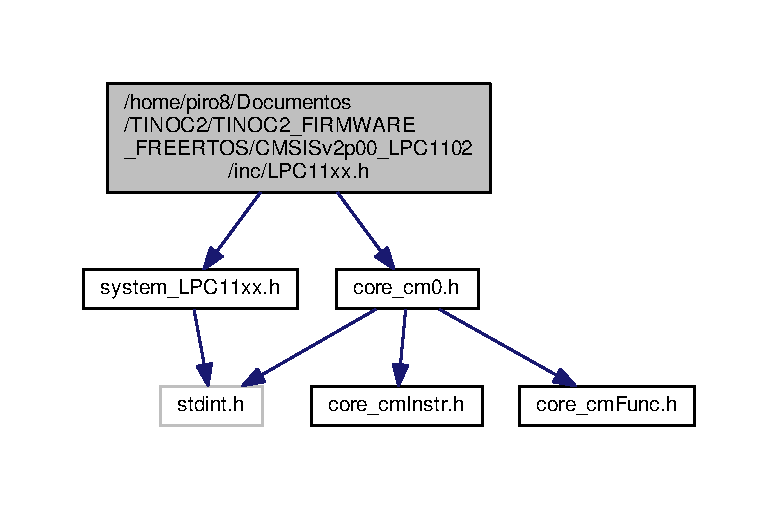
\includegraphics[width=350pt]{_l_p_c11xx_8h__incl}
\end{center}
\end{figure}
This graph shows which files directly or indirectly include this file\+:\nopagebreak
\begin{figure}[H]
\begin{center}
\leavevmode
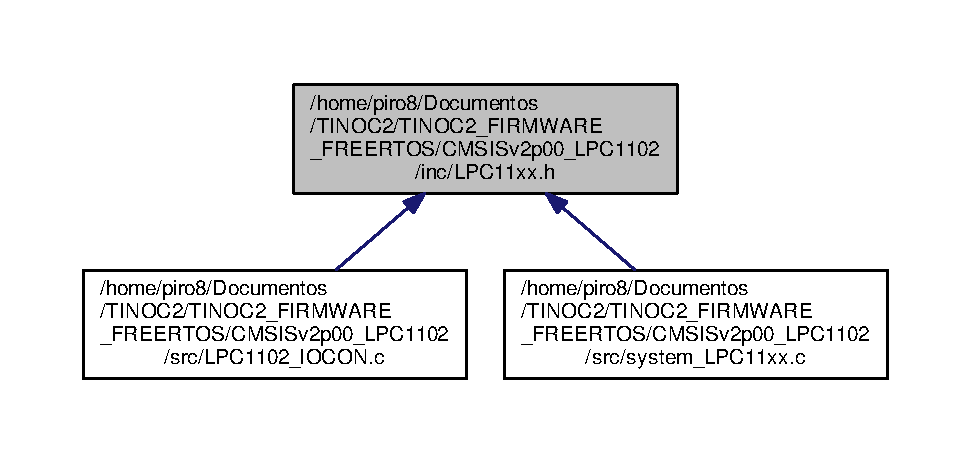
\includegraphics[width=350pt]{_l_p_c11xx_8h__dep__incl}
\end{center}
\end{figure}
\subsection*{Classes}
\begin{DoxyCompactItemize}
\item 
struct \hyperlink{struct_l_p_c___s_y_s_c_o_n___type_def}{L\+P\+C\+\_\+\+S\+Y\+S\+C\+O\+N\+\_\+\+Type\+Def}
\item 
struct \hyperlink{struct_l_p_c___i_o_c_o_n___type_def}{L\+P\+C\+\_\+\+I\+O\+C\+O\+N\+\_\+\+Type\+Def}
\item 
struct \hyperlink{struct_l_p_c___p_m_u___type_def}{L\+P\+C\+\_\+\+P\+M\+U\+\_\+\+Type\+Def}
\item 
struct \hyperlink{struct_l_p_c___f_l_a_s_h_c_t_r_l___type}{L\+P\+C\+\_\+\+F\+L\+A\+S\+H\+C\+T\+R\+L\+\_\+\+Type}
\item 
struct \hyperlink{struct_l_p_c___g_p_i_o___type_def}{L\+P\+C\+\_\+\+G\+P\+I\+O\+\_\+\+Type\+Def}
\item 
struct \hyperlink{struct_l_p_c___t_m_r___type_def}{L\+P\+C\+\_\+\+T\+M\+R\+\_\+\+Type\+Def}
\item 
struct \hyperlink{struct_l_p_c___u_a_r_t___type_def}{L\+P\+C\+\_\+\+U\+A\+R\+T\+\_\+\+Type\+Def}
\item 
struct \hyperlink{struct_l_p_c___s_s_p___type_def}{L\+P\+C\+\_\+\+S\+S\+P\+\_\+\+Type\+Def}
\item 
struct \hyperlink{struct_l_p_c___i2_c___type_def}{L\+P\+C\+\_\+\+I2\+C\+\_\+\+Type\+Def}
\item 
struct \hyperlink{struct_l_p_c___w_d_t___type_def}{L\+P\+C\+\_\+\+W\+D\+T\+\_\+\+Type\+Def}
\item 
struct \hyperlink{struct_l_p_c___a_d_c___type_def}{L\+P\+C\+\_\+\+A\+D\+C\+\_\+\+Type\+Def}
\item 
struct \hyperlink{struct_l_p_c___c_a_n___type_def}{L\+P\+C\+\_\+\+C\+A\+N\+\_\+\+Type\+Def}
\end{DoxyCompactItemize}
\subsection*{Macros}
\begin{DoxyCompactItemize}
\item 
\#define \hyperlink{group___l_p_c11xx___c_m_s_i_s_ga4127d1b31aaf336fab3d7329d117f448}{\+\_\+\+\_\+\+M\+P\+U\+\_\+\+P\+R\+E\+S\+E\+NT}~0
\item 
\#define \hyperlink{group___l_p_c11xx___c_m_s_i_s_gae3fe3587d5100c787e02102ce3944460}{\+\_\+\+\_\+\+N\+V\+I\+C\+\_\+\+P\+R\+I\+O\+\_\+\+B\+I\+TS}~2
\item 
\#define \hyperlink{group___l_p_c11xx___c_m_s_i_s_gab58771b4ec03f9bdddc84770f7c95c68}{\+\_\+\+\_\+\+Vendor\+\_\+\+Sys\+Tick\+Config}~0
\item 
\#define \hyperlink{group___l_p_c11xx___definitions_ga7d7417b6cd6c6975fa03de03920d27e8}{L\+P\+C\+\_\+\+F\+L\+A\+S\+H\+\_\+\+B\+A\+SE}~(0x00000000\+U\+L)
\item 
\#define \hyperlink{group___l_p_c11xx___definitions_ga9782814ad6434f200b65440d2ac01c2a}{L\+P\+C\+\_\+\+R\+A\+M\+\_\+\+B\+A\+SE}~(0x10000000\+U\+L)
\item 
\#define \hyperlink{group___l_p_c11xx___definitions_ga55cab996c3594a0f4cc459ec8e10daea}{L\+P\+C\+\_\+\+A\+P\+B0\+\_\+\+B\+A\+SE}~(0x40000000\+U\+L)
\item 
\#define \hyperlink{group___l_p_c11xx___definitions_ga8e0d25ffe3428ed27f963e83089046a8}{L\+P\+C\+\_\+\+A\+H\+B\+\_\+\+B\+A\+SE}~(0x50000000\+U\+L)
\item 
\#define \hyperlink{group___l_p_c11xx___definitions_ga9e53652929424015ade23fe30e1d022b}{L\+P\+C\+\_\+\+I2\+C\+\_\+\+B\+A\+SE}~(\hyperlink{group___l_p_c11xx___definitions_ga55cab996c3594a0f4cc459ec8e10daea}{L\+P\+C\+\_\+\+A\+P\+B0\+\_\+\+B\+A\+SE} + 0x00000)
\item 
\#define \hyperlink{group___l_p_c11xx___definitions_ga02a30b0be4672972c3af9e5aebdcfea1}{L\+P\+C\+\_\+\+W\+D\+T\+\_\+\+B\+A\+SE}~(\hyperlink{group___l_p_c11xx___definitions_ga55cab996c3594a0f4cc459ec8e10daea}{L\+P\+C\+\_\+\+A\+P\+B0\+\_\+\+B\+A\+SE} + 0x04000)
\item 
\#define \hyperlink{group___l_p_c11xx___definitions_ga50ba023c2b0046a5be8b1b236effeb35}{L\+P\+C\+\_\+\+U\+A\+R\+T\+\_\+\+B\+A\+SE}~(\hyperlink{group___l_p_c11xx___definitions_ga55cab996c3594a0f4cc459ec8e10daea}{L\+P\+C\+\_\+\+A\+P\+B0\+\_\+\+B\+A\+SE} + 0x08000)
\item 
\#define \hyperlink{group___l_p_c11xx___definitions_ga663c7a2d9c286efce1fd9c90c0068dac}{L\+P\+C\+\_\+\+C\+T16\+B0\+\_\+\+B\+A\+SE}~(\hyperlink{group___l_p_c11xx___definitions_ga55cab996c3594a0f4cc459ec8e10daea}{L\+P\+C\+\_\+\+A\+P\+B0\+\_\+\+B\+A\+SE} + 0x0\+C000)
\item 
\#define \hyperlink{group___l_p_c11xx___definitions_ga5f33f849b010785defa0105cf6eb87f1}{L\+P\+C\+\_\+\+C\+T16\+B1\+\_\+\+B\+A\+SE}~(\hyperlink{group___l_p_c11xx___definitions_ga55cab996c3594a0f4cc459ec8e10daea}{L\+P\+C\+\_\+\+A\+P\+B0\+\_\+\+B\+A\+SE} + 0x10000)
\item 
\#define \hyperlink{group___l_p_c11xx___definitions_ga10dcc3ac224bf132010cb6bc6fc7d9c9}{L\+P\+C\+\_\+\+C\+T32\+B0\+\_\+\+B\+A\+SE}~(\hyperlink{group___l_p_c11xx___definitions_ga55cab996c3594a0f4cc459ec8e10daea}{L\+P\+C\+\_\+\+A\+P\+B0\+\_\+\+B\+A\+SE} + 0x14000)
\item 
\#define \hyperlink{group___l_p_c11xx___definitions_ga70f807832b5a2afb17265d22fed6160d}{L\+P\+C\+\_\+\+C\+T32\+B1\+\_\+\+B\+A\+SE}~(\hyperlink{group___l_p_c11xx___definitions_ga55cab996c3594a0f4cc459ec8e10daea}{L\+P\+C\+\_\+\+A\+P\+B0\+\_\+\+B\+A\+SE} + 0x18000)
\item 
\#define \hyperlink{group___l_p_c11xx___definitions_ga2396e0d0c565e4c1c3b2fc593bd6c37f}{L\+P\+C\+\_\+\+A\+D\+C\+\_\+\+B\+A\+SE}~(\hyperlink{group___l_p_c11xx___definitions_ga55cab996c3594a0f4cc459ec8e10daea}{L\+P\+C\+\_\+\+A\+P\+B0\+\_\+\+B\+A\+SE} + 0x1\+C000)
\item 
\#define \hyperlink{group___l_p_c11xx___definitions_ga865bed8ad61e9e273439ad1349a46d68}{L\+P\+C\+\_\+\+P\+M\+U\+\_\+\+B\+A\+SE}~(\hyperlink{group___l_p_c11xx___definitions_ga55cab996c3594a0f4cc459ec8e10daea}{L\+P\+C\+\_\+\+A\+P\+B0\+\_\+\+B\+A\+SE} + 0x38000)
\item 
\#define \hyperlink{group___l_p_c11xx___definitions_gad8bd09a830e15ea80293576f61deeccd}{L\+P\+C\+\_\+\+F\+L\+A\+S\+H\+C\+T\+R\+L\+\_\+\+B\+A\+SE}~(\hyperlink{group___l_p_c11xx___definitions_ga55cab996c3594a0f4cc459ec8e10daea}{L\+P\+C\+\_\+\+A\+P\+B0\+\_\+\+B\+A\+SE} + 0x3\+C000)
\item 
\#define \hyperlink{group___l_p_c11xx___definitions_ga53fb1af80b541545988f2a966681abfd}{L\+P\+C\+\_\+\+S\+S\+P0\+\_\+\+B\+A\+SE}~(\hyperlink{group___l_p_c11xx___definitions_ga55cab996c3594a0f4cc459ec8e10daea}{L\+P\+C\+\_\+\+A\+P\+B0\+\_\+\+B\+A\+SE} + 0x40000)
\item 
\#define \hyperlink{group___l_p_c11xx___definitions_gae48aea115d5924805263d7a15402d4fa}{L\+P\+C\+\_\+\+I\+O\+C\+O\+N\+\_\+\+B\+A\+SE}~(\hyperlink{group___l_p_c11xx___definitions_ga55cab996c3594a0f4cc459ec8e10daea}{L\+P\+C\+\_\+\+A\+P\+B0\+\_\+\+B\+A\+SE} + 0x44000)
\item 
\#define \hyperlink{group___l_p_c11xx___definitions_ga976cd83a81fd89a472221e68f0c0fbff}{L\+P\+C\+\_\+\+S\+Y\+S\+C\+O\+N\+\_\+\+B\+A\+SE}~(\hyperlink{group___l_p_c11xx___definitions_ga55cab996c3594a0f4cc459ec8e10daea}{L\+P\+C\+\_\+\+A\+P\+B0\+\_\+\+B\+A\+SE} + 0x48000)
\item 
\#define \hyperlink{group___l_p_c11xx___definitions_gaeae0f80f43f37b41a8a1c3cb7028d22f}{L\+P\+C\+\_\+\+C\+A\+N\+\_\+\+B\+A\+SE}~(\hyperlink{group___l_p_c11xx___definitions_ga55cab996c3594a0f4cc459ec8e10daea}{L\+P\+C\+\_\+\+A\+P\+B0\+\_\+\+B\+A\+SE} + 0x50000)
\item 
\#define \hyperlink{group___l_p_c11xx___definitions_ga05d118997f53f596d3a087f8b91a1969}{L\+P\+C\+\_\+\+S\+S\+P1\+\_\+\+B\+A\+SE}~(\hyperlink{group___l_p_c11xx___definitions_ga55cab996c3594a0f4cc459ec8e10daea}{L\+P\+C\+\_\+\+A\+P\+B0\+\_\+\+B\+A\+SE} + 0x58000)
\item 
\#define \hyperlink{group___l_p_c11xx___definitions_ga5feb4a6692784a25eaed627661bd8f36}{L\+P\+C\+\_\+\+G\+P\+I\+O\+\_\+\+B\+A\+SE}~(\hyperlink{group___l_p_c11xx___definitions_ga8e0d25ffe3428ed27f963e83089046a8}{L\+P\+C\+\_\+\+A\+H\+B\+\_\+\+B\+A\+SE}  + 0x00000)
\item 
\#define \hyperlink{group___l_p_c11xx___definitions_ga09e0e964ea1abf3b991772df2aa52405}{L\+P\+C\+\_\+\+G\+P\+I\+O0\+\_\+\+B\+A\+SE}~(\hyperlink{group___l_p_c11xx___definitions_ga8e0d25ffe3428ed27f963e83089046a8}{L\+P\+C\+\_\+\+A\+H\+B\+\_\+\+B\+A\+SE}  + 0x00000)
\item 
\#define \hyperlink{group___l_p_c11xx___definitions_ga9fb0536853721a3073bd69d94d0b7ec2}{L\+P\+C\+\_\+\+G\+P\+I\+O1\+\_\+\+B\+A\+SE}~(\hyperlink{group___l_p_c11xx___definitions_ga8e0d25ffe3428ed27f963e83089046a8}{L\+P\+C\+\_\+\+A\+H\+B\+\_\+\+B\+A\+SE}  + 0x10000)
\item 
\#define \hyperlink{group___l_p_c11xx___definitions_gae5524b2d728167194033ec7a1841a36b}{L\+P\+C\+\_\+\+G\+P\+I\+O2\+\_\+\+B\+A\+SE}~(\hyperlink{group___l_p_c11xx___definitions_ga8e0d25ffe3428ed27f963e83089046a8}{L\+P\+C\+\_\+\+A\+H\+B\+\_\+\+B\+A\+SE}  + 0x20000)
\item 
\#define \hyperlink{group___l_p_c11xx___definitions_ga56c68c5326b521b3278a35f4d81369a9}{L\+P\+C\+\_\+\+G\+P\+I\+O3\+\_\+\+B\+A\+SE}~(\hyperlink{group___l_p_c11xx___definitions_ga8e0d25ffe3428ed27f963e83089046a8}{L\+P\+C\+\_\+\+A\+H\+B\+\_\+\+B\+A\+SE}  + 0x30000)
\item 
\#define \hyperlink{group___l_p_c11xx___definitions_ga70a2faf2e119737f0e660984564d4907}{L\+P\+C\+\_\+\+I2C}~((\hyperlink{struct_l_p_c___i2_c___type_def}{L\+P\+C\+\_\+\+I2\+C\+\_\+\+Type\+Def}    $\ast$) \hyperlink{group___l_p_c11xx___definitions_ga9e53652929424015ade23fe30e1d022b}{L\+P\+C\+\_\+\+I2\+C\+\_\+\+B\+A\+SE}   )
\item 
\#define \hyperlink{group___l_p_c11xx___definitions_ga7d68cf0829652bd8c1f837c697653c5f}{L\+P\+C\+\_\+\+W\+DT}~((\hyperlink{struct_l_p_c___w_d_t___type_def}{L\+P\+C\+\_\+\+W\+D\+T\+\_\+\+Type\+Def}    $\ast$) \hyperlink{group___l_p_c11xx___definitions_ga02a30b0be4672972c3af9e5aebdcfea1}{L\+P\+C\+\_\+\+W\+D\+T\+\_\+\+B\+A\+SE}   )
\item 
\#define \hyperlink{group___l_p_c11xx___definitions_ga31a69c06776f4a82569d7ed7e91bd45c}{L\+P\+C\+\_\+\+U\+A\+RT}~((\hyperlink{struct_l_p_c___u_a_r_t___type_def}{L\+P\+C\+\_\+\+U\+A\+R\+T\+\_\+\+Type\+Def}   $\ast$) \hyperlink{group___l_p_c11xx___definitions_ga50ba023c2b0046a5be8b1b236effeb35}{L\+P\+C\+\_\+\+U\+A\+R\+T\+\_\+\+B\+A\+SE}  )
\item 
\#define \hyperlink{group___l_p_c11xx___definitions_gae3e75d39e502088028bfe901b28f6471}{L\+P\+C\+\_\+\+T\+M\+R16\+B0}~((\hyperlink{struct_l_p_c___t_m_r___type_def}{L\+P\+C\+\_\+\+T\+M\+R\+\_\+\+Type\+Def}    $\ast$) \hyperlink{group___l_p_c11xx___definitions_ga663c7a2d9c286efce1fd9c90c0068dac}{L\+P\+C\+\_\+\+C\+T16\+B0\+\_\+\+B\+A\+SE})
\item 
\#define \hyperlink{group___l_p_c11xx___definitions_gad82d36f91fa86aad5e3d57f5543e4cf6}{L\+P\+C\+\_\+\+T\+M\+R16\+B1}~((\hyperlink{struct_l_p_c___t_m_r___type_def}{L\+P\+C\+\_\+\+T\+M\+R\+\_\+\+Type\+Def}    $\ast$) \hyperlink{group___l_p_c11xx___definitions_ga5f33f849b010785defa0105cf6eb87f1}{L\+P\+C\+\_\+\+C\+T16\+B1\+\_\+\+B\+A\+SE})
\item 
\#define \hyperlink{group___l_p_c11xx___definitions_ga59694d96a23b3e6de134dc5f34ad61e8}{L\+P\+C\+\_\+\+T\+M\+R32\+B0}~((\hyperlink{struct_l_p_c___t_m_r___type_def}{L\+P\+C\+\_\+\+T\+M\+R\+\_\+\+Type\+Def}    $\ast$) \hyperlink{group___l_p_c11xx___definitions_ga10dcc3ac224bf132010cb6bc6fc7d9c9}{L\+P\+C\+\_\+\+C\+T32\+B0\+\_\+\+B\+A\+SE})
\item 
\#define \hyperlink{group___l_p_c11xx___definitions_gab5cca8bad611399aad1da65cfafcbe2e}{L\+P\+C\+\_\+\+T\+M\+R32\+B1}~((\hyperlink{struct_l_p_c___t_m_r___type_def}{L\+P\+C\+\_\+\+T\+M\+R\+\_\+\+Type\+Def}    $\ast$) \hyperlink{group___l_p_c11xx___definitions_ga70f807832b5a2afb17265d22fed6160d}{L\+P\+C\+\_\+\+C\+T32\+B1\+\_\+\+B\+A\+SE})
\item 
\#define \hyperlink{group___l_p_c11xx___definitions_gab6eaf639d3a1eec83583a9e11ab7336f}{L\+P\+C\+\_\+\+A\+DC}~((\hyperlink{struct_l_p_c___a_d_c___type_def}{L\+P\+C\+\_\+\+A\+D\+C\+\_\+\+Type\+Def}    $\ast$) \hyperlink{group___l_p_c11xx___definitions_ga2396e0d0c565e4c1c3b2fc593bd6c37f}{L\+P\+C\+\_\+\+A\+D\+C\+\_\+\+B\+A\+SE}   )
\item 
\#define \hyperlink{group___l_p_c11xx___definitions_ga9d540cc313db00679c10f9ac1961b06a}{L\+P\+C\+\_\+\+P\+MU}~((\hyperlink{struct_l_p_c___p_m_u___type_def}{L\+P\+C\+\_\+\+P\+M\+U\+\_\+\+Type\+Def}    $\ast$) \hyperlink{group___l_p_c11xx___definitions_ga865bed8ad61e9e273439ad1349a46d68}{L\+P\+C\+\_\+\+P\+M\+U\+\_\+\+B\+A\+SE}   )
\item 
\#define \hyperlink{group___l_p_c11xx___definitions_ga0e5b0ed0e4ad1155df98372c932e8bc7}{L\+P\+C\+\_\+\+F\+L\+A\+S\+H\+C\+T\+RL}~((\hyperlink{struct_l_p_c___f_l_a_s_h_c_t_r_l___type}{L\+P\+C\+\_\+\+F\+L\+A\+S\+H\+C\+T\+R\+L\+\_\+\+Type} $\ast$) \hyperlink{group___l_p_c11xx___definitions_gad8bd09a830e15ea80293576f61deeccd}{L\+P\+C\+\_\+\+F\+L\+A\+S\+H\+C\+T\+R\+L\+\_\+\+B\+A\+SE})
\item 
\#define \hyperlink{group___l_p_c11xx___definitions_gac213e0325a8e8a972bd2e0dd6ccf353c}{L\+P\+C\+\_\+\+S\+S\+P0}~((\hyperlink{struct_l_p_c___s_s_p___type_def}{L\+P\+C\+\_\+\+S\+S\+P\+\_\+\+Type\+Def}    $\ast$) \hyperlink{group___l_p_c11xx___definitions_ga53fb1af80b541545988f2a966681abfd}{L\+P\+C\+\_\+\+S\+S\+P0\+\_\+\+B\+A\+SE}  )
\item 
\#define \hyperlink{group___l_p_c11xx___definitions_ga09c4610ada1d9aa18913963cbd1a6e52}{L\+P\+C\+\_\+\+S\+S\+P1}~((\hyperlink{struct_l_p_c___s_s_p___type_def}{L\+P\+C\+\_\+\+S\+S\+P\+\_\+\+Type\+Def}    $\ast$) \hyperlink{group___l_p_c11xx___definitions_ga05d118997f53f596d3a087f8b91a1969}{L\+P\+C\+\_\+\+S\+S\+P1\+\_\+\+B\+A\+SE}  )
\item 
\#define \hyperlink{group___l_p_c11xx___definitions_ga177aa5b075c24ed459e92f4698bea9cc}{L\+P\+C\+\_\+\+C\+AN}~((\hyperlink{struct_l_p_c___c_a_n___type_def}{L\+P\+C\+\_\+\+C\+A\+N\+\_\+\+Type\+Def}    $\ast$) \hyperlink{group___l_p_c11xx___definitions_gaeae0f80f43f37b41a8a1c3cb7028d22f}{L\+P\+C\+\_\+\+C\+A\+N\+\_\+\+B\+A\+SE}   )
\item 
\#define \hyperlink{group___l_p_c11xx___definitions_gaabc651799ba17b0dd4a0114c8d48a145}{L\+P\+C\+\_\+\+I\+O\+C\+ON}~((\hyperlink{struct_l_p_c___i_o_c_o_n___type_def}{L\+P\+C\+\_\+\+I\+O\+C\+O\+N\+\_\+\+Type\+Def}  $\ast$) \hyperlink{group___l_p_c11xx___definitions_gae48aea115d5924805263d7a15402d4fa}{L\+P\+C\+\_\+\+I\+O\+C\+O\+N\+\_\+\+B\+A\+SE} )
\item 
\#define \hyperlink{group___l_p_c11xx___definitions_gabe45c10a979fe812e3d9ecd72fe33a2f}{L\+P\+C\+\_\+\+S\+Y\+S\+C\+ON}~((\hyperlink{struct_l_p_c___s_y_s_c_o_n___type_def}{L\+P\+C\+\_\+\+S\+Y\+S\+C\+O\+N\+\_\+\+Type\+Def} $\ast$) \hyperlink{group___l_p_c11xx___definitions_ga976cd83a81fd89a472221e68f0c0fbff}{L\+P\+C\+\_\+\+S\+Y\+S\+C\+O\+N\+\_\+\+B\+A\+SE})
\item 
\#define \hyperlink{group___l_p_c11xx___definitions_ga92f3de6ff5cfd5b8c290696fad07b18a}{L\+P\+C\+\_\+\+G\+P\+I\+O0}~((\hyperlink{struct_l_p_c___g_p_i_o___type_def}{L\+P\+C\+\_\+\+G\+P\+I\+O\+\_\+\+Type\+Def}   $\ast$) \hyperlink{group___l_p_c11xx___definitions_ga09e0e964ea1abf3b991772df2aa52405}{L\+P\+C\+\_\+\+G\+P\+I\+O0\+\_\+\+B\+A\+SE} )
\item 
\#define \hyperlink{group___l_p_c11xx___definitions_ga335587dad4e6d0da56c1f3ad1c087d10}{L\+P\+C\+\_\+\+G\+P\+I\+O1}~((\hyperlink{struct_l_p_c___g_p_i_o___type_def}{L\+P\+C\+\_\+\+G\+P\+I\+O\+\_\+\+Type\+Def}   $\ast$) \hyperlink{group___l_p_c11xx___definitions_ga9fb0536853721a3073bd69d94d0b7ec2}{L\+P\+C\+\_\+\+G\+P\+I\+O1\+\_\+\+B\+A\+SE} )
\item 
\#define \hyperlink{group___l_p_c11xx___definitions_ga27a09e8c08f9e209c6af70b0a3c56b39}{L\+P\+C\+\_\+\+G\+P\+I\+O2}~((\hyperlink{struct_l_p_c___g_p_i_o___type_def}{L\+P\+C\+\_\+\+G\+P\+I\+O\+\_\+\+Type\+Def}   $\ast$) \hyperlink{group___l_p_c11xx___definitions_gae5524b2d728167194033ec7a1841a36b}{L\+P\+C\+\_\+\+G\+P\+I\+O2\+\_\+\+B\+A\+SE} )
\item 
\#define \hyperlink{group___l_p_c11xx___definitions_ga6e961eb01d0f1e61dd9b9d5979d2aafc}{L\+P\+C\+\_\+\+G\+P\+I\+O3}~((\hyperlink{struct_l_p_c___g_p_i_o___type_def}{L\+P\+C\+\_\+\+G\+P\+I\+O\+\_\+\+Type\+Def}   $\ast$) \hyperlink{group___l_p_c11xx___definitions_ga56c68c5326b521b3278a35f4d81369a9}{L\+P\+C\+\_\+\+G\+P\+I\+O3\+\_\+\+B\+A\+SE} )
\end{DoxyCompactItemize}
\subsection*{Typedefs}
\begin{DoxyCompactItemize}
\item 
typedef enum \hyperlink{group___l_p_c11xx___c_m_s_i_s_ga666eb0caeb12ec0e281415592ae89083}{I\+R\+Qn} \hyperlink{group___l_p_c11xx___c_m_s_i_s_gac3af4a32370fb28c4ade8bf2add80251}{I\+R\+Qn\+\_\+\+Type}
\end{DoxyCompactItemize}
\subsection*{Enumerations}
\begin{DoxyCompactItemize}
\item 
enum \hyperlink{group___l_p_c11xx___c_m_s_i_s_ga666eb0caeb12ec0e281415592ae89083}{I\+R\+Qn} \{ \\*
\hyperlink{group___l_p_c11xx___c_m_s_i_s_gga666eb0caeb12ec0e281415592ae89083ade177d9c70c89e084093024b932a4e30}{Non\+Maskable\+Int\+\_\+\+I\+R\+Qn} = -\/14, 
\hyperlink{group___l_p_c11xx___c_m_s_i_s_gga666eb0caeb12ec0e281415592ae89083ab1a222a34a32f0ef5ac65e714efc1f85}{Hard\+Fault\+\_\+\+I\+R\+Qn} = -\/13, 
\hyperlink{group___l_p_c11xx___c_m_s_i_s_gga666eb0caeb12ec0e281415592ae89083a4ce820b3cc6cf3a796b41aadc0cf1237}{S\+V\+Call\+\_\+\+I\+R\+Qn} = -\/5, 
\hyperlink{group___l_p_c11xx___c_m_s_i_s_gga666eb0caeb12ec0e281415592ae89083a03c3cc89984928816d81793fc7bce4a2}{Pend\+S\+V\+\_\+\+I\+R\+Qn} = -\/2, 
\\*
\hyperlink{group___l_p_c11xx___c_m_s_i_s_gga666eb0caeb12ec0e281415592ae89083a6dbff8f8543325f3474cbae2446776e7}{Sys\+Tick\+\_\+\+I\+R\+Qn} = -\/1, 
\hyperlink{group___l_p_c11xx___c_m_s_i_s_gga666eb0caeb12ec0e281415592ae89083af01060170ceb0d6d577beacf41635ae0}{W\+A\+K\+E\+U\+P0\+\_\+\+I\+R\+Qn} = 0, 
\hyperlink{group___l_p_c11xx___c_m_s_i_s_gga666eb0caeb12ec0e281415592ae89083ad8e04985fa950d0759ce92d557a7ed7f}{W\+A\+K\+E\+U\+P1\+\_\+\+I\+R\+Qn} = 1, 
\hyperlink{group___l_p_c11xx___c_m_s_i_s_gga666eb0caeb12ec0e281415592ae89083ad4b2bb0ae5c1d52381f8cb9413affbf6}{W\+A\+K\+E\+U\+P2\+\_\+\+I\+R\+Qn} = 2, 
\\*
\hyperlink{group___l_p_c11xx___c_m_s_i_s_gga666eb0caeb12ec0e281415592ae89083a539f4e76913e12d41c7eec2e7c2239ed}{W\+A\+K\+E\+U\+P3\+\_\+\+I\+R\+Qn} = 3, 
\hyperlink{group___l_p_c11xx___c_m_s_i_s_gga666eb0caeb12ec0e281415592ae89083a3df13a5d451b495e0a86647b0750a837}{W\+A\+K\+E\+U\+P4\+\_\+\+I\+R\+Qn} = 4, 
\hyperlink{group___l_p_c11xx___c_m_s_i_s_gga666eb0caeb12ec0e281415592ae89083a3dfaf99bdb7c4b21bbc6a5e65d62ce5a}{W\+A\+K\+E\+U\+P5\+\_\+\+I\+R\+Qn} = 5, 
\hyperlink{group___l_p_c11xx___c_m_s_i_s_gga666eb0caeb12ec0e281415592ae89083ace715bb711cdb57694878d18789989a5}{W\+A\+K\+E\+U\+P6\+\_\+\+I\+R\+Qn} = 6, 
\\*
\hyperlink{group___l_p_c11xx___c_m_s_i_s_gga666eb0caeb12ec0e281415592ae89083a06b94ece7d467d84b4706956fbe9dc43}{W\+A\+K\+E\+U\+P7\+\_\+\+I\+R\+Qn} = 7, 
\hyperlink{group___l_p_c11xx___c_m_s_i_s_gga666eb0caeb12ec0e281415592ae89083ac84fd704de6c04930319dcc12c630698}{W\+A\+K\+E\+U\+P8\+\_\+\+I\+R\+Qn} = 8, 
\hyperlink{group___l_p_c11xx___c_m_s_i_s_gga666eb0caeb12ec0e281415592ae89083aa91c95e855a44d1d5c0b92ff2b979051}{W\+A\+K\+E\+U\+P9\+\_\+\+I\+R\+Qn} = 9, 
\hyperlink{group___l_p_c11xx___c_m_s_i_s_gga666eb0caeb12ec0e281415592ae89083a85209d0ff16184ac86dfdb01d8b26502}{W\+A\+K\+E\+U\+P10\+\_\+\+I\+R\+Qn} = 10, 
\\*
\hyperlink{group___l_p_c11xx___c_m_s_i_s_gga666eb0caeb12ec0e281415592ae89083a4f3db149d5fbb1513aa3c5e3fe9e7356}{W\+A\+K\+E\+U\+P11\+\_\+\+I\+R\+Qn} = 11, 
\hyperlink{group___l_p_c11xx___c_m_s_i_s_gga666eb0caeb12ec0e281415592ae89083a5595570597adb716c29763e5d5a2f484}{W\+A\+K\+E\+U\+P12\+\_\+\+I\+R\+Qn} = 12, 
\hyperlink{group___l_p_c11xx___c_m_s_i_s_gga666eb0caeb12ec0e281415592ae89083a20d0bdfa1654b723493895e3ea617cdb}{C\+A\+N\+\_\+\+I\+R\+Qn} = 13, 
\hyperlink{group___l_p_c11xx___c_m_s_i_s_gga666eb0caeb12ec0e281415592ae89083adcc0cfa46f0d13c2de0f3e826c10a789}{S\+S\+P1\+\_\+\+I\+R\+Qn} = 14, 
\\*
\hyperlink{group___l_p_c11xx___c_m_s_i_s_gga666eb0caeb12ec0e281415592ae89083adf8c31fe1c7ade2eb05f1414710dbce7}{I2\+C\+\_\+\+I\+R\+Qn} = 15, 
\hyperlink{group___l_p_c11xx___c_m_s_i_s_gga666eb0caeb12ec0e281415592ae89083a6f5ed57785374cb1ba3a1256e0d991be}{T\+I\+M\+E\+R\+\_\+16\+\_\+0\+\_\+\+I\+R\+Qn} = 16, 
\hyperlink{group___l_p_c11xx___c_m_s_i_s_gga666eb0caeb12ec0e281415592ae89083a9d13f0d0bbeb7bc1c75d512a94d66c9f}{T\+I\+M\+E\+R\+\_\+16\+\_\+1\+\_\+\+I\+R\+Qn} = 17, 
\hyperlink{group___l_p_c11xx___c_m_s_i_s_gga666eb0caeb12ec0e281415592ae89083a7e40673d4557974606b5d9670c0c50d0}{T\+I\+M\+E\+R\+\_\+32\+\_\+0\+\_\+\+I\+R\+Qn} = 18, 
\\*
\hyperlink{group___l_p_c11xx___c_m_s_i_s_gga666eb0caeb12ec0e281415592ae89083ac178a073454f598a32b7f95bcaba7679}{T\+I\+M\+E\+R\+\_\+32\+\_\+1\+\_\+\+I\+R\+Qn} = 19, 
\hyperlink{group___l_p_c11xx___c_m_s_i_s_gga666eb0caeb12ec0e281415592ae89083a6c8d6262fd7ecedc57b2fe9209be9765}{S\+S\+P0\+\_\+\+I\+R\+Qn} = 20, 
\hyperlink{group___l_p_c11xx___c_m_s_i_s_gga666eb0caeb12ec0e281415592ae89083a9d9be6e918c912367e393dae3480eabb}{U\+A\+R\+T\+\_\+\+I\+R\+Qn} = 21, 
\hyperlink{group___l_p_c11xx___c_m_s_i_s_gga666eb0caeb12ec0e281415592ae89083a2095f58b6c0de45b782b1196a0939e02}{Reserved0\+\_\+\+I\+R\+Qn} = 22, 
\\*
\hyperlink{group___l_p_c11xx___c_m_s_i_s_gga666eb0caeb12ec0e281415592ae89083add6253fd238cff7fa4b35e4ef81ffc07}{Reserved1\+\_\+\+I\+R\+Qn} = 23, 
\hyperlink{group___l_p_c11xx___c_m_s_i_s_gga666eb0caeb12ec0e281415592ae89083a4d69175258ae261dd545001e810421b3}{A\+D\+C\+\_\+\+I\+R\+Qn} = 24, 
\hyperlink{group___l_p_c11xx___c_m_s_i_s_gga666eb0caeb12ec0e281415592ae89083a78573b84a4133ef5812b33ce10dcba12}{W\+D\+T\+\_\+\+I\+R\+Qn} = 25, 
\hyperlink{group___l_p_c11xx___c_m_s_i_s_gga666eb0caeb12ec0e281415592ae89083ac2ee5960aed41ff349aa7a86c37e9ab2}{B\+O\+D\+\_\+\+I\+R\+Qn} = 26, 
\\*
\hyperlink{group___l_p_c11xx___c_m_s_i_s_gga666eb0caeb12ec0e281415592ae89083ab58dc79a081058857f73965f5305479b}{F\+M\+C\+\_\+\+I\+R\+Qn} = 27, 
\hyperlink{group___l_p_c11xx___c_m_s_i_s_gga666eb0caeb12ec0e281415592ae89083a14098dd2e0d0331c1e5f1f80dde14371}{E\+I\+N\+T3\+\_\+\+I\+R\+Qn} = 28, 
\hyperlink{group___l_p_c11xx___c_m_s_i_s_gga666eb0caeb12ec0e281415592ae89083a40ab356422a691418668d6bbfd9f17b9}{E\+I\+N\+T2\+\_\+\+I\+R\+Qn} = 29, 
\hyperlink{group___l_p_c11xx___c_m_s_i_s_gga666eb0caeb12ec0e281415592ae89083ad855ae101e21a04054a9844066900d7c}{E\+I\+N\+T1\+\_\+\+I\+R\+Qn} = 30, 
\\*
\hyperlink{group___l_p_c11xx___c_m_s_i_s_gga666eb0caeb12ec0e281415592ae89083a0a3db3233549f012f8ecb88f0510adcf}{E\+I\+N\+T0\+\_\+\+I\+R\+Qn} = 31
 \}
\end{DoxyCompactItemize}

\hypertarget{system___l_p_c11xx_8h}{}\section{/home/piro8/\+Documentos/\+T\+I\+N\+O\+C2/\+T\+I\+N\+O\+C2\+\_\+\+F\+I\+R\+M\+W\+A\+R\+E\+\_\+\+F\+R\+E\+E\+R\+T\+O\+S/\+C\+M\+S\+I\+Sv2p00\+\_\+\+L\+P\+C1102/inc/system\+\_\+\+L\+P\+C11xx.h File Reference}
\label{system___l_p_c11xx_8h}\index{/home/piro8/\+Documentos/\+T\+I\+N\+O\+C2/\+T\+I\+N\+O\+C2\+\_\+\+F\+I\+R\+M\+W\+A\+R\+E\+\_\+\+F\+R\+E\+E\+R\+T\+O\+S/\+C\+M\+S\+I\+Sv2p00\+\_\+\+L\+P\+C1102/inc/system\+\_\+\+L\+P\+C11xx.\+h@{/home/piro8/\+Documentos/\+T\+I\+N\+O\+C2/\+T\+I\+N\+O\+C2\+\_\+\+F\+I\+R\+M\+W\+A\+R\+E\+\_\+\+F\+R\+E\+E\+R\+T\+O\+S/\+C\+M\+S\+I\+Sv2p00\+\_\+\+L\+P\+C1102/inc/system\+\_\+\+L\+P\+C11xx.\+h}}


C\+M\+S\+IS Cortex-\/\+M0 Device Peripheral Access Layer Header File for the N\+XP L\+P\+C11xx Device Series.  


{\ttfamily \#include $<$stdint.\+h$>$}\\*
Include dependency graph for system\+\_\+\+L\+P\+C11xx.\+h\+:\nopagebreak
\begin{figure}[H]
\begin{center}
\leavevmode
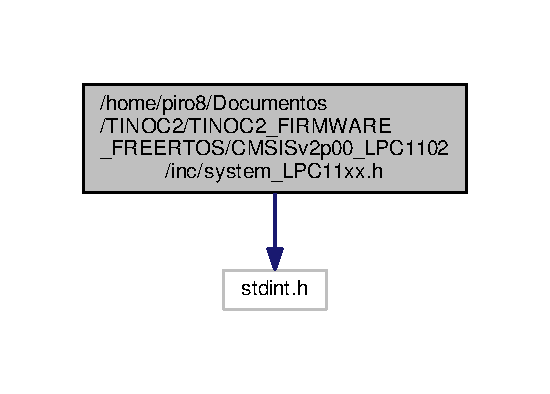
\includegraphics[width=264pt]{system___l_p_c11xx_8h__incl}
\end{center}
\end{figure}
This graph shows which files directly or indirectly include this file\+:\nopagebreak
\begin{figure}[H]
\begin{center}
\leavevmode
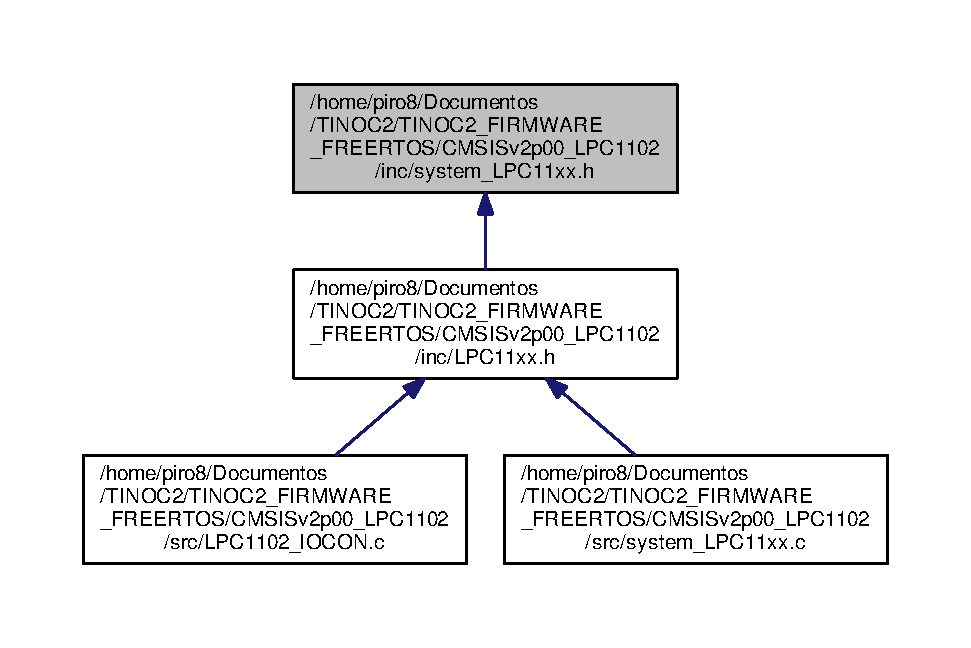
\includegraphics[width=350pt]{system___l_p_c11xx_8h__dep__incl}
\end{center}
\end{figure}
\subsection*{Functions}
\begin{DoxyCompactItemize}
\item 
void \hyperlink{system___l_p_c11xx_8h_a93f514700ccf00d08dbdcff7f1224eb2}{System\+Init} (void)
\begin{DoxyCompactList}\small\item\em Setup the microcontroller system. Initialize the System and update the System\+Core\+Clock variable. \end{DoxyCompactList}\item 
void \hyperlink{system___l_p_c11xx_8h_ae0c36a9591fe6e9c45ecb21a794f0f0f}{System\+Core\+Clock\+Update} (void)
\begin{DoxyCompactList}\small\item\em Updates the System\+Core\+Clock with current core Clock retrieved from cpu registers. \end{DoxyCompactList}\end{DoxyCompactItemize}
\subsection*{Variables}
\begin{DoxyCompactItemize}
\item 
uint32\+\_\+t \hyperlink{system___l_p_c11xx_8h_aa3cd3e43291e81e795d642b79b6088e6}{System\+Core\+Clock}
\end{DoxyCompactItemize}


\subsection{Detailed Description}
C\+M\+S\+IS Cortex-\/\+M0 Device Peripheral Access Layer Header File for the N\+XP L\+P\+C11xx Device Series. 

\begin{DoxyVersion}{Version}
V1.\+00 
\end{DoxyVersion}
\begin{DoxyDate}{Date}
17. November 2009
\end{DoxyDate}
\begin{DoxyNote}{Note}
Copyright (C) 2009 A\+RM Limited. All rights reserved.
\end{DoxyNote}
\begin{DoxyParagraph}{}
A\+RM Limited (A\+RM) is supplying this software for use with Cortex-\/M processor based microcontrollers. This file can be freely distributed within development tools that are supporting such A\+RM based processors.
\end{DoxyParagraph}
\begin{DoxyParagraph}{}
T\+H\+IS S\+O\+F\+T\+W\+A\+RE IS P\+R\+O\+V\+I\+D\+ED \char`\"{}\+A\+S I\+S\char`\"{}. NO W\+A\+R\+R\+A\+N\+T\+I\+ES, W\+H\+E\+T\+H\+ER E\+X\+P\+R\+E\+SS, I\+M\+P\+L\+I\+ED OR S\+T\+A\+T\+U\+T\+O\+RY, I\+N\+C\+L\+U\+D\+I\+NG, B\+UT N\+OT L\+I\+M\+I\+T\+ED TO, I\+M\+P\+L\+I\+ED W\+A\+R\+R\+A\+N\+T\+I\+ES OF M\+E\+R\+C\+H\+A\+N\+T\+A\+B\+I\+L\+I\+TY A\+ND F\+I\+T\+N\+E\+SS F\+OR A P\+A\+R\+T\+I\+C\+U\+L\+AR P\+U\+R\+P\+O\+SE A\+P\+P\+LY TO T\+H\+IS S\+O\+F\+T\+W\+A\+RE. A\+RM S\+H\+A\+LL N\+OT, IN A\+NY C\+I\+R\+C\+U\+M\+S\+T\+A\+N\+C\+ES, BE L\+I\+A\+B\+LE F\+OR S\+P\+E\+C\+I\+AL, I\+N\+C\+I\+D\+E\+N\+T\+AL, OR C\+O\+N\+S\+E\+Q\+U\+E\+N\+T\+I\+AL D\+A\+M\+A\+G\+ES, F\+OR A\+NY R\+E\+A\+S\+ON W\+H\+A\+T\+S\+O\+E\+V\+ER. 
\end{DoxyParagraph}


\subsection{Function Documentation}
\index{system\+\_\+\+L\+P\+C11xx.\+h@{system\+\_\+\+L\+P\+C11xx.\+h}!System\+Core\+Clock\+Update@{System\+Core\+Clock\+Update}}
\index{System\+Core\+Clock\+Update@{System\+Core\+Clock\+Update}!system\+\_\+\+L\+P\+C11xx.\+h@{system\+\_\+\+L\+P\+C11xx.\+h}}
\subsubsection[{\texorpdfstring{System\+Core\+Clock\+Update(void)}{SystemCoreClockUpdate(void)}}]{\setlength{\rightskip}{0pt plus 5cm}void System\+Core\+Clock\+Update (
\begin{DoxyParamCaption}
\item[{void}]{}
\end{DoxyParamCaption}
)}\hypertarget{system___l_p_c11xx_8h_ae0c36a9591fe6e9c45ecb21a794f0f0f}{}\label{system___l_p_c11xx_8h_ae0c36a9591fe6e9c45ecb21a794f0f0f}


Updates the System\+Core\+Clock with current core Clock retrieved from cpu registers. 

Update System\+Core\+Clock variable


\begin{DoxyParams}{Parameters}
{\em none} & \\
\hline
\end{DoxyParams}
\begin{DoxyReturn}{Returns}
none 
\end{DoxyReturn}


Definition at line 323 of file system\+\_\+\+L\+P\+C11xx.\+c.

\index{system\+\_\+\+L\+P\+C11xx.\+h@{system\+\_\+\+L\+P\+C11xx.\+h}!System\+Init@{System\+Init}}
\index{System\+Init@{System\+Init}!system\+\_\+\+L\+P\+C11xx.\+h@{system\+\_\+\+L\+P\+C11xx.\+h}}
\subsubsection[{\texorpdfstring{System\+Init(void)}{SystemInit(void)}}]{\setlength{\rightskip}{0pt plus 5cm}void System\+Init (
\begin{DoxyParamCaption}
\item[{void}]{}
\end{DoxyParamCaption}
)}\hypertarget{system___l_p_c11xx_8h_a93f514700ccf00d08dbdcff7f1224eb2}{}\label{system___l_p_c11xx_8h_a93f514700ccf00d08dbdcff7f1224eb2}


Setup the microcontroller system. Initialize the System and update the System\+Core\+Clock variable. 

Initialize the system


\begin{DoxyParams}{Parameters}
{\em none} & \\
\hline
\end{DoxyParams}
\begin{DoxyReturn}{Returns}
none
\end{DoxyReturn}
Setup the microcontroller system. Initialize the System and update the System\+Core\+Clock variable.

Initialize the system


\begin{DoxyParams}{Parameters}
{\em none} & \\
\hline
\end{DoxyParams}
\begin{DoxyReturn}{Returns}
none 
\end{DoxyReturn}


Definition at line 414 of file system\+\_\+\+L\+P\+C11xx.\+c.



\subsection{Variable Documentation}
\index{system\+\_\+\+L\+P\+C11xx.\+h@{system\+\_\+\+L\+P\+C11xx.\+h}!System\+Core\+Clock@{System\+Core\+Clock}}
\index{System\+Core\+Clock@{System\+Core\+Clock}!system\+\_\+\+L\+P\+C11xx.\+h@{system\+\_\+\+L\+P\+C11xx.\+h}}
\subsubsection[{\texorpdfstring{System\+Core\+Clock}{SystemCoreClock}}]{\setlength{\rightskip}{0pt plus 5cm}uint32\+\_\+t System\+Core\+Clock}\hypertarget{system___l_p_c11xx_8h_aa3cd3e43291e81e795d642b79b6088e6}{}\label{system___l_p_c11xx_8h_aa3cd3e43291e81e795d642b79b6088e6}
System Clock Frequency (Core Clock) 

Definition at line 317 of file system\+\_\+\+L\+P\+C11xx.\+c.


\hypertarget{core__cm0_8c}{}\section{/home/piro8/\+Documentos/\+T\+I\+N\+O\+C2/\+T\+I\+N\+O\+C2\+\_\+\+F\+I\+R\+M\+W\+A\+R\+E\+\_\+\+F\+R\+E\+E\+R\+T\+O\+S/\+C\+M\+S\+I\+Sv2p00\+\_\+\+L\+P\+C1102/src/core\+\_\+cm0.c File Reference}
\label{core__cm0_8c}\index{/home/piro8/\+Documentos/\+T\+I\+N\+O\+C2/\+T\+I\+N\+O\+C2\+\_\+\+F\+I\+R\+M\+W\+A\+R\+E\+\_\+\+F\+R\+E\+E\+R\+T\+O\+S/\+C\+M\+S\+I\+Sv2p00\+\_\+\+L\+P\+C1102/src/core\+\_\+cm0.\+c@{/home/piro8/\+Documentos/\+T\+I\+N\+O\+C2/\+T\+I\+N\+O\+C2\+\_\+\+F\+I\+R\+M\+W\+A\+R\+E\+\_\+\+F\+R\+E\+E\+R\+T\+O\+S/\+C\+M\+S\+I\+Sv2p00\+\_\+\+L\+P\+C1102/src/core\+\_\+cm0.\+c}}


C\+M\+S\+IS Cortex-\/\+M0 Core Peripheral Access Layer Source File.  


{\ttfamily \#include $<$stdint.\+h$>$}\\*
Include dependency graph for core\+\_\+cm0.\+c\+:\nopagebreak
\begin{figure}[H]
\begin{center}
\leavevmode
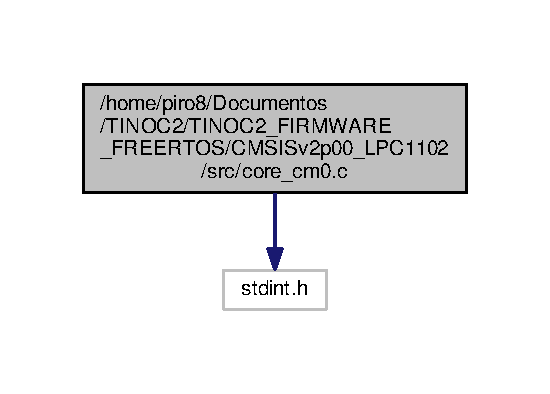
\includegraphics[width=264pt]{core__cm0_8c__incl}
\end{center}
\end{figure}


\subsection{Detailed Description}
C\+M\+S\+IS Cortex-\/\+M0 Core Peripheral Access Layer Source File. 

\begin{DoxyVersion}{Version}
V2.\+00 
\end{DoxyVersion}
\begin{DoxyDate}{Date}
10. September 2010
\end{DoxyDate}
\begin{DoxyNote}{Note}
Copyright (C) 2009-\/2010 A\+RM Limited. All rights reserved.
\end{DoxyNote}
\begin{DoxyParagraph}{}
A\+RM Limited (A\+RM) is supplying this software for use with Cortex-\/M processor based microcontrollers. This file can be freely distributed within development tools that are supporting such A\+RM based processors.
\end{DoxyParagraph}
\begin{DoxyParagraph}{}
T\+H\+IS S\+O\+F\+T\+W\+A\+RE IS P\+R\+O\+V\+I\+D\+ED \char`\"{}\+A\+S I\+S\char`\"{}. NO W\+A\+R\+R\+A\+N\+T\+I\+ES, W\+H\+E\+T\+H\+ER E\+X\+P\+R\+E\+SS, I\+M\+P\+L\+I\+ED OR S\+T\+A\+T\+U\+T\+O\+RY, I\+N\+C\+L\+U\+D\+I\+NG, B\+UT N\+OT L\+I\+M\+I\+T\+ED TO, I\+M\+P\+L\+I\+ED W\+A\+R\+R\+A\+N\+T\+I\+ES OF M\+E\+R\+C\+H\+A\+N\+T\+A\+B\+I\+L\+I\+TY A\+ND F\+I\+T\+N\+E\+SS F\+OR A P\+A\+R\+T\+I\+C\+U\+L\+AR P\+U\+R\+P\+O\+SE A\+P\+P\+LY TO T\+H\+IS S\+O\+F\+T\+W\+A\+RE. A\+RM S\+H\+A\+LL N\+OT, IN A\+NY C\+I\+R\+C\+U\+M\+S\+T\+A\+N\+C\+ES, BE L\+I\+A\+B\+LE F\+OR S\+P\+E\+C\+I\+AL, I\+N\+C\+I\+D\+E\+N\+T\+AL, OR C\+O\+N\+S\+E\+Q\+U\+E\+N\+T\+I\+AL D\+A\+M\+A\+G\+ES, F\+OR A\+NY R\+E\+A\+S\+ON W\+H\+A\+T\+S\+O\+E\+V\+ER. 
\end{DoxyParagraph}

\hypertarget{_l_p_c1102___i_o_c_o_n_8c}{}\section{/home/piro8/\+Documentos/\+T\+I\+N\+O\+C2/\+T\+I\+N\+O\+C2\+\_\+\+F\+I\+R\+M\+W\+A\+R\+E\+\_\+\+F\+R\+E\+E\+R\+T\+O\+S/\+C\+M\+S\+I\+Sv2p00\+\_\+\+L\+P\+C1102/src/\+L\+P\+C1102\+\_\+\+I\+O\+C\+ON.c File Reference}
\label{_l_p_c1102___i_o_c_o_n_8c}\index{/home/piro8/\+Documentos/\+T\+I\+N\+O\+C2/\+T\+I\+N\+O\+C2\+\_\+\+F\+I\+R\+M\+W\+A\+R\+E\+\_\+\+F\+R\+E\+E\+R\+T\+O\+S/\+C\+M\+S\+I\+Sv2p00\+\_\+\+L\+P\+C1102/src/\+L\+P\+C1102\+\_\+\+I\+O\+C\+O\+N.\+c@{/home/piro8/\+Documentos/\+T\+I\+N\+O\+C2/\+T\+I\+N\+O\+C2\+\_\+\+F\+I\+R\+M\+W\+A\+R\+E\+\_\+\+F\+R\+E\+E\+R\+T\+O\+S/\+C\+M\+S\+I\+Sv2p00\+\_\+\+L\+P\+C1102/src/\+L\+P\+C1102\+\_\+\+I\+O\+C\+O\+N.\+c}}


Archivo de funciones del registro I\+O\+C\+ON.  


{\ttfamily \#include $<$stdint.\+h$>$}\\*
{\ttfamily \#include $<$L\+P\+C11xx.\+h$>$}\\*
{\ttfamily \#include $<$core\+\_\+cm0.\+h$>$}\\*
{\ttfamily \#include $<$L\+P\+C1102\+\_\+\+I\+O\+C\+O\+N.\+h$>$}\\*
Include dependency graph for L\+P\+C1102\+\_\+\+I\+O\+C\+O\+N.\+c\+:\nopagebreak
\begin{figure}[H]
\begin{center}
\leavevmode
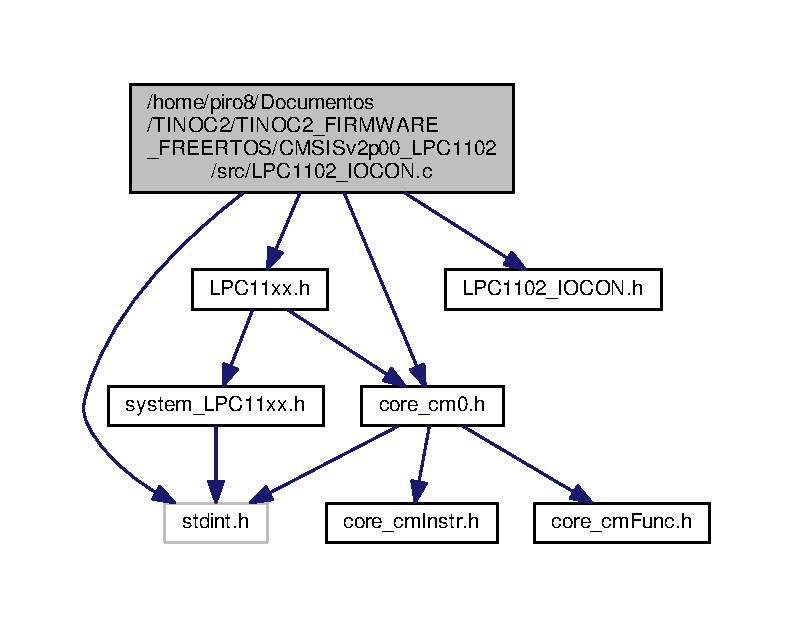
\includegraphics[width=350pt]{_l_p_c1102___i_o_c_o_n_8c__incl}
\end{center}
\end{figure}
\subsection*{Functions}
\begin{DoxyCompactItemize}
\item 
uint8\+\_\+t \hyperlink{_l_p_c1102___i_o_c_o_n_8c_af75b3cee3837ed7b38752ba092d61932}{Definir\+\_\+\+Pin\+\_\+\+Configuracion\+\_\+\+IO} (\hyperlink{_l_p_c1102___i_o_c_o_n_8h_ac86bf230dbe0f6c26abfc86c49b1952e}{t\+\_\+pin} pin, uint32\+\_\+t funcion, uint32\+\_\+t modo, uint32\+\_\+t histeresis, uint32\+\_\+t opendrain)
\begin{DoxyCompactList}\small\item\em Definición de la configuración de un pin. \end{DoxyCompactList}\end{DoxyCompactItemize}


\subsection{Detailed Description}
Archivo de funciones del registro I\+O\+C\+ON. 

Manejo de campos y funciones del registro I\+O\+C\+ON~\newline
U\+M10429 Capitulo 7\+: L\+P\+C1102/04 I/O Configuration \begin{DoxyAuthor}{Author}
Roux, Federico G. (\href{mailto:froux@favaloro.edu.ar}{\tt froux@favaloro.\+edu.\+ar}) 
\end{DoxyAuthor}


\subsection{Function Documentation}
\index{L\+P\+C1102\+\_\+\+I\+O\+C\+O\+N.\+c@{L\+P\+C1102\+\_\+\+I\+O\+C\+O\+N.\+c}!Definir\+\_\+\+Pin\+\_\+\+Configuracion\+\_\+\+IO@{Definir\+\_\+\+Pin\+\_\+\+Configuracion\+\_\+\+IO}}
\index{Definir\+\_\+\+Pin\+\_\+\+Configuracion\+\_\+\+IO@{Definir\+\_\+\+Pin\+\_\+\+Configuracion\+\_\+\+IO}!L\+P\+C1102\+\_\+\+I\+O\+C\+O\+N.\+c@{L\+P\+C1102\+\_\+\+I\+O\+C\+O\+N.\+c}}
\subsubsection[{\texorpdfstring{Definir\+\_\+\+Pin\+\_\+\+Configuracion\+\_\+\+I\+O(t\+\_\+pin pin, uint32\+\_\+t funcion, uint32\+\_\+t modo, uint32\+\_\+t histeresis, uint32\+\_\+t opendrain)}{Definir_Pin_Configuracion_IO(t_pin pin, uint32_t funcion, uint32_t modo, uint32_t histeresis, uint32_t opendrain)}}]{\setlength{\rightskip}{0pt plus 5cm}uint8\+\_\+t Definir\+\_\+\+Pin\+\_\+\+Configuracion\+\_\+\+IO (
\begin{DoxyParamCaption}
\item[{{\bf t\+\_\+pin}}]{pin, }
\item[{uint32\+\_\+t}]{funcion, }
\item[{uint32\+\_\+t}]{modo, }
\item[{uint32\+\_\+t}]{histeresis, }
\item[{uint32\+\_\+t}]{opendrain}
\end{DoxyParamCaption}
)}\hypertarget{_l_p_c1102___i_o_c_o_n_8c_af75b3cee3837ed7b38752ba092d61932}{}\label{_l_p_c1102___i_o_c_o_n_8c_af75b3cee3837ed7b38752ba092d61932}


Definición de la configuración de un pin. 

\hyperlink{_l_p_c1102___i_o_c_o_n_8c_af75b3cee3837ed7b38752ba092d61932}{Definir\+\_\+\+Pin\+\_\+\+Configuracion\+\_\+\+I\+O()}


\begin{DoxyParams}[1]{Parameters}
\mbox{\tt in}  & {\em pin} & Listado de pines disponibles del microcontrolador. Ver \+: \hyperlink{group___l_p_c___i_o_c_o_n___l_p_c1102___p_i_n_e_s}{L\+P\+C\+\_\+\+I\+O\+C\+O\+N\+\_\+\+L\+P\+C1102\+\_\+\+P\+I\+N\+ES} \\
\hline
\mbox{\tt in}  & {\em modo} & Modo de resistencia\+: inactivo, pull-\/up, pull-\/down, repetidor. Ver\+: \hyperlink{group___l_p_c___i_o_c_o_n___l_p_c1102___m_o_d_e}{L\+P\+C\+\_\+\+I\+O\+C\+O\+N\+\_\+\+L\+P\+C1102\+\_\+\+M\+O\+DE} \\
\hline
\mbox{\tt in}  & {\em histeresis} & Bit de activacion de histeresis. Ver \+: \hyperlink{group___l_p_c___i_o_c_o_n___l_p_c1102___h_y_s___o_d}{L\+P\+C\+\_\+\+I\+O\+C\+O\+N\+\_\+\+L\+P\+C1102\+\_\+\+H\+Y\+S\+\_\+\+OD} \\
\hline
\mbox{\tt in}  & {\em opendrain} & Bit de activacion de salida opendrain. Ver \+: \hyperlink{group___l_p_c___i_o_c_o_n___l_p_c1102___h_y_s___o_d}{L\+P\+C\+\_\+\+I\+O\+C\+O\+N\+\_\+\+L\+P\+C1102\+\_\+\+H\+Y\+S\+\_\+\+OD} \\
\hline
\end{DoxyParams}


Definition at line 39 of file L\+P\+C1102\+\_\+\+I\+O\+C\+O\+N.\+c.


\hypertarget{system___l_p_c11xx_8c}{}\section{/home/piro8/\+Documentos/\+T\+I\+N\+O\+C2/\+T\+I\+N\+O\+C2\+\_\+\+F\+I\+R\+M\+W\+A\+R\+E\+\_\+\+F\+R\+E\+E\+R\+T\+O\+S/\+C\+M\+S\+I\+Sv2p00\+\_\+\+L\+P\+C1102/src/system\+\_\+\+L\+P\+C11xx.c File Reference}
\label{system___l_p_c11xx_8c}\index{/home/piro8/\+Documentos/\+T\+I\+N\+O\+C2/\+T\+I\+N\+O\+C2\+\_\+\+F\+I\+R\+M\+W\+A\+R\+E\+\_\+\+F\+R\+E\+E\+R\+T\+O\+S/\+C\+M\+S\+I\+Sv2p00\+\_\+\+L\+P\+C1102/src/system\+\_\+\+L\+P\+C11xx.\+c@{/home/piro8/\+Documentos/\+T\+I\+N\+O\+C2/\+T\+I\+N\+O\+C2\+\_\+\+F\+I\+R\+M\+W\+A\+R\+E\+\_\+\+F\+R\+E\+E\+R\+T\+O\+S/\+C\+M\+S\+I\+Sv2p00\+\_\+\+L\+P\+C1102/src/system\+\_\+\+L\+P\+C11xx.\+c}}


C\+M\+S\+IS Cortex-\/\+M0 Device Peripheral Access Layer Source File for the N\+XP L\+P\+C11xx Device Series.  


{\ttfamily \#include $<$stdint.\+h$>$}\\*
{\ttfamily \#include \char`\"{}L\+P\+C11xx.\+h\char`\"{}}\\*
Include dependency graph for system\+\_\+\+L\+P\+C11xx.\+c\+:\nopagebreak
\begin{figure}[H]
\begin{center}
\leavevmode
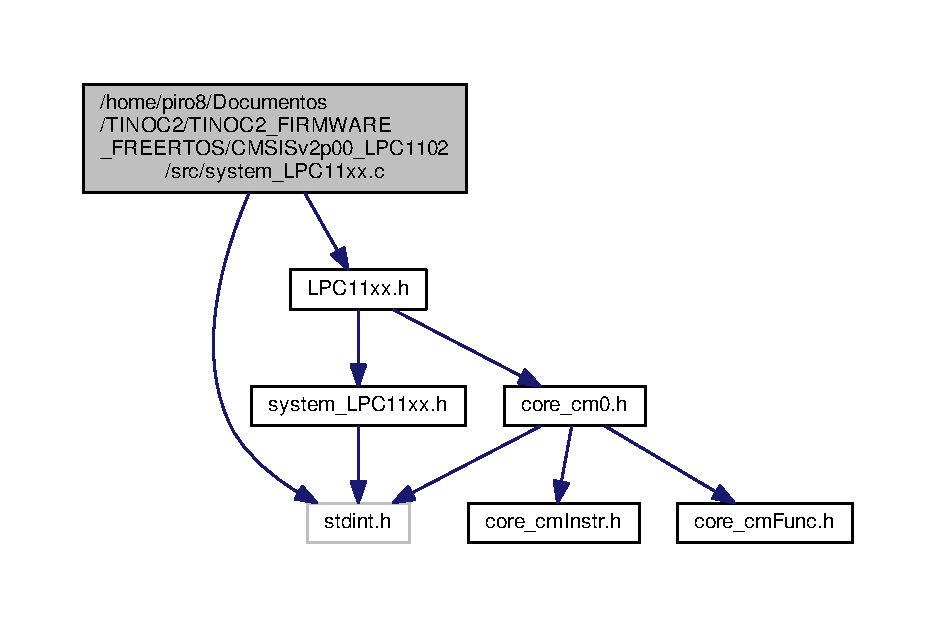
\includegraphics[width=350pt]{system___l_p_c11xx_8c__incl}
\end{center}
\end{figure}
\subsection*{Macros}
\begin{DoxyCompactItemize}
\item 
\#define \hyperlink{system___l_p_c11xx_8c_aee2245fb4caf68f0fc571d8b24ff5626}{C\+L\+O\+C\+K\+\_\+\+S\+E\+T\+UP}~1
\item 
\#define \hyperlink{system___l_p_c11xx_8c_a778179c3b51f6c717d3f4720e9863b9a}{S\+Y\+S\+C\+L\+K\+\_\+\+S\+E\+T\+UP}~1
\item 
\#define \hyperlink{system___l_p_c11xx_8c_ae468fce354573a1c79b5d95feb9faf4f}{S\+Y\+S\+O\+S\+C\+\_\+\+S\+E\+T\+UP}~1
\item 
\#define \hyperlink{system___l_p_c11xx_8c_a76890281b6f6a4b25f1b0e7e37baf53e}{S\+Y\+S\+O\+S\+C\+C\+T\+R\+L\+\_\+\+Val}~0x00000000
\item 
\#define \hyperlink{system___l_p_c11xx_8c_a84abebab829b8bfac13a2fa9b84f141e}{W\+D\+T\+O\+S\+C\+\_\+\+S\+E\+T\+UP}~0
\item 
\#define \hyperlink{system___l_p_c11xx_8c_a1135febcbc334b18f5a85820db085abd}{W\+D\+T\+O\+S\+C\+C\+T\+R\+L\+\_\+\+Val}~0x000000\+A0
\item 
\#define \hyperlink{system___l_p_c11xx_8c_a91d26ac1bf14f9b612f13c6ae89e4a40}{S\+Y\+S\+P\+L\+L\+C\+L\+K\+S\+E\+L\+\_\+\+Val}~0x00000000
\item 
\#define \hyperlink{system___l_p_c11xx_8c_a7ae9a76d3d25029032d53e92baaf183a}{S\+Y\+S\+P\+L\+L\+\_\+\+S\+E\+T\+UP}~1
\item 
\#define \hyperlink{system___l_p_c11xx_8c_aa3cef1360b564acd1c3f947debaae5b8}{S\+Y\+S\+P\+L\+L\+C\+T\+R\+L\+\_\+\+Val}~0x00000023
\item 
\#define \hyperlink{system___l_p_c11xx_8c_a797720f5a22b83184675441f771e42df}{M\+A\+I\+N\+C\+L\+K\+S\+E\+L\+\_\+\+Val}~0x00000000
\item 
\#define \hyperlink{system___l_p_c11xx_8c_a7c86ce9b0526f914ed4a13ac94c37fa1}{S\+Y\+S\+A\+H\+B\+C\+L\+K\+D\+I\+V\+\_\+\+Val}~0x00000001
\item 
\#define \hyperlink{system___l_p_c11xx_8c_ae2e3b021e3356e1f5638ac896a360533}{A\+H\+B\+C\+L\+K\+C\+T\+R\+L\+\_\+\+Val}~0x0001005F
\item 
\#define \hyperlink{system___l_p_c11xx_8c_a3d498490bb1e408b61c1bc4363e2764b}{S\+S\+P0\+C\+L\+K\+D\+I\+V\+\_\+\+Val}~0x00000001
\item 
\#define \hyperlink{system___l_p_c11xx_8c_aab78254bf0012c8d711d174eb1f472b2}{U\+A\+R\+T\+C\+L\+K\+D\+I\+V\+\_\+\+Val}~0x00000001
\item 
\#define \hyperlink{system___l_p_c11xx_8c_a7f0e9dff667e1dcc98dbc63cf495b653}{S\+S\+P1\+C\+L\+K\+D\+I\+V\+\_\+\+Val}~0x00000001
\item 
\#define \hyperlink{system___l_p_c11xx_8c_a208d2aa3957a550ac9a7c2579cdf70f4}{M\+E\+M\+M\+A\+P\+\_\+\+S\+E\+T\+UP}~0
\item 
\#define \hyperlink{system___l_p_c11xx_8c_a6548d18fbd7a29750139ced6b0b68dfa}{S\+Y\+S\+M\+E\+M\+R\+E\+M\+A\+P\+\_\+\+Val}~0x00000001
\item 
\#define \hyperlink{system___l_p_c11xx_8c_a773c8761088ae68a786a4c72bb42deec}{C\+H\+E\+C\+K\+\_\+\+R\+A\+N\+GE}(val,  min,  max)~((val $<$ min) $\vert$$\vert$ (val $>$ max))
\item 
\#define \hyperlink{system___l_p_c11xx_8c_a098e4b07ffb372fafb9aefd1a2393136}{C\+H\+E\+C\+K\+\_\+\+R\+S\+VD}(val,  mask)~(val \& mask)
\item 
\#define \hyperlink{system___l_p_c11xx_8c_a8687edecd98881631a879bd10528c7da}{\+\_\+\+\_\+\+X\+T\+AL}~(12000000\+U\+L)    /$\ast$ Oscillator frequency             $\ast$/
\item 
\#define \hyperlink{system___l_p_c11xx_8c_ab759225f52a45a9f898ec8c4a5dfecc8}{\+\_\+\+\_\+\+S\+Y\+S\+\_\+\+O\+S\+C\+\_\+\+C\+LK}~(    \hyperlink{system___l_p_c11xx_8c_a8687edecd98881631a879bd10528c7da}{\+\_\+\+\_\+\+X\+T\+AL})    /$\ast$ Main oscillator frequency        $\ast$/
\item 
\#define \hyperlink{system___l_p_c11xx_8c_a6834fd34cd023b03d5ec210b029a4a0a}{\+\_\+\+\_\+\+I\+R\+C\+\_\+\+O\+S\+C\+\_\+\+C\+LK}~(12000000\+U\+L)    /$\ast$ Internal R\+C oscillator frequency $\ast$/
\item 
\#define \hyperlink{system___l_p_c11xx_8c_a4bcab3c5ea93b388cc0a337e7eec893a}{\+\_\+\+\_\+\+F\+R\+E\+Q\+S\+EL}~((\hyperlink{system___l_p_c11xx_8c_a1135febcbc334b18f5a85820db085abd}{W\+D\+T\+O\+S\+C\+C\+T\+R\+L\+\_\+\+Val} $>$$>$ 5) \& 0x0\+F)
\item 
\#define \hyperlink{system___l_p_c11xx_8c_ab915f35929843ff914d818ba64fb2c6b}{\+\_\+\+\_\+\+D\+I\+V\+S\+EL}~(((\hyperlink{system___l_p_c11xx_8c_a1135febcbc334b18f5a85820db085abd}{W\+D\+T\+O\+S\+C\+C\+T\+R\+L\+\_\+\+Val} \& 0x1\+F) $<$$<$ 1) + 2)
\item 
\#define \hyperlink{system___l_p_c11xx_8c_a63e69efa838dca1a81a549bd3786ec32}{\+\_\+\+\_\+\+W\+D\+T\+\_\+\+O\+S\+C\+\_\+\+C\+LK}~(1600000 / 2)
\item 
\#define \hyperlink{system___l_p_c11xx_8c_a02586b58cc1d3dcf06ad87c645ccce21}{\+\_\+\+\_\+\+S\+Y\+S\+\_\+\+P\+L\+L\+C\+L\+K\+IN}~(\hyperlink{system___l_p_c11xx_8c_a6834fd34cd023b03d5ec210b029a4a0a}{\+\_\+\+\_\+\+I\+R\+C\+\_\+\+O\+S\+C\+\_\+\+C\+LK})
\item 
\#define \hyperlink{system___l_p_c11xx_8c_a17e860407d0495e261ccfd4c1d662151}{\+\_\+\+\_\+\+S\+Y\+S\+\_\+\+P\+L\+L\+C\+L\+K\+O\+UT}~(\hyperlink{system___l_p_c11xx_8c_a02586b58cc1d3dcf06ad87c645ccce21}{\+\_\+\+\_\+\+S\+Y\+S\+\_\+\+P\+L\+L\+C\+L\+K\+IN} $\ast$ ((\hyperlink{system___l_p_c11xx_8c_aa3cef1360b564acd1c3f947debaae5b8}{S\+Y\+S\+P\+L\+L\+C\+T\+R\+L\+\_\+\+Val} \& 0x01\+F) + 1))
\item 
\#define \hyperlink{system___l_p_c11xx_8c_a358f14b51ccee88ceeb868c94a398886}{\+\_\+\+\_\+\+M\+A\+I\+N\+\_\+\+C\+L\+O\+CK}~(\hyperlink{system___l_p_c11xx_8c_a6834fd34cd023b03d5ec210b029a4a0a}{\+\_\+\+\_\+\+I\+R\+C\+\_\+\+O\+S\+C\+\_\+\+C\+LK})
\item 
\#define \hyperlink{system___l_p_c11xx_8c_a16323f44d2b5b11ef3972f71339cbd39}{\+\_\+\+\_\+\+S\+Y\+S\+T\+E\+M\+\_\+\+C\+L\+O\+CK}~(\hyperlink{system___l_p_c11xx_8c_a358f14b51ccee88ceeb868c94a398886}{\+\_\+\+\_\+\+M\+A\+I\+N\+\_\+\+C\+L\+O\+CK} / \hyperlink{system___l_p_c11xx_8c_a7c86ce9b0526f914ed4a13ac94c37fa1}{S\+Y\+S\+A\+H\+B\+C\+L\+K\+D\+I\+V\+\_\+\+Val})
\end{DoxyCompactItemize}
\subsection*{Functions}
\begin{DoxyCompactItemize}
\item 
void \hyperlink{system___l_p_c11xx_8c_ae0c36a9591fe6e9c45ecb21a794f0f0f}{System\+Core\+Clock\+Update} (void)
\begin{DoxyCompactList}\small\item\em Updates the System\+Core\+Clock with current core Clock retrieved from cpu registers. \end{DoxyCompactList}\item 
void \hyperlink{system___l_p_c11xx_8c_a93f514700ccf00d08dbdcff7f1224eb2}{System\+Init} (void)
\begin{DoxyCompactList}\small\item\em Setup the microcontroller system. Initialize the System. \end{DoxyCompactList}\end{DoxyCompactItemize}
\subsection*{Variables}
\begin{DoxyCompactItemize}
\item 
uint32\+\_\+t \hyperlink{system___l_p_c11xx_8c_aa3cd3e43291e81e795d642b79b6088e6}{System\+Core\+Clock} = \hyperlink{system___l_p_c11xx_8c_a16323f44d2b5b11ef3972f71339cbd39}{\+\_\+\+\_\+\+S\+Y\+S\+T\+E\+M\+\_\+\+C\+L\+O\+CK}
\end{DoxyCompactItemize}


\subsection{Detailed Description}
C\+M\+S\+IS Cortex-\/\+M0 Device Peripheral Access Layer Source File for the N\+XP L\+P\+C11xx Device Series. 

\begin{DoxyVersion}{Version}
V1.\+00 
\end{DoxyVersion}
\begin{DoxyDate}{Date}
17. November 2009
\end{DoxyDate}
\begin{DoxyNote}{Note}
Copyright (C) 2009 A\+RM Limited. All rights reserved.
\end{DoxyNote}
\begin{DoxyParagraph}{}
A\+RM Limited (A\+RM) is supplying this software for use with Cortex-\/M processor based microcontrollers. This file can be freely distributed within development tools that are supporting such A\+RM based processors.
\end{DoxyParagraph}
\begin{DoxyParagraph}{}
T\+H\+IS S\+O\+F\+T\+W\+A\+RE IS P\+R\+O\+V\+I\+D\+ED \char`\"{}\+A\+S I\+S\char`\"{}. NO W\+A\+R\+R\+A\+N\+T\+I\+ES, W\+H\+E\+T\+H\+ER E\+X\+P\+R\+E\+SS, I\+M\+P\+L\+I\+ED OR S\+T\+A\+T\+U\+T\+O\+RY, I\+N\+C\+L\+U\+D\+I\+NG, B\+UT N\+OT L\+I\+M\+I\+T\+ED TO, I\+M\+P\+L\+I\+ED W\+A\+R\+R\+A\+N\+T\+I\+ES OF M\+E\+R\+C\+H\+A\+N\+T\+A\+B\+I\+L\+I\+TY A\+ND F\+I\+T\+N\+E\+SS F\+OR A P\+A\+R\+T\+I\+C\+U\+L\+AR P\+U\+R\+P\+O\+SE A\+P\+P\+LY TO T\+H\+IS S\+O\+F\+T\+W\+A\+RE. A\+RM S\+H\+A\+LL N\+OT, IN A\+NY C\+I\+R\+C\+U\+M\+S\+T\+A\+N\+C\+ES, BE L\+I\+A\+B\+LE F\+OR S\+P\+E\+C\+I\+AL, I\+N\+C\+I\+D\+E\+N\+T\+AL, OR C\+O\+N\+S\+E\+Q\+U\+E\+N\+T\+I\+AL D\+A\+M\+A\+G\+ES, F\+OR A\+NY R\+E\+A\+S\+ON W\+H\+A\+T\+S\+O\+E\+V\+ER. 
\end{DoxyParagraph}


\subsection{Macro Definition Documentation}
\index{system\+\_\+\+L\+P\+C11xx.\+c@{system\+\_\+\+L\+P\+C11xx.\+c}!\+\_\+\+\_\+\+D\+I\+V\+S\+EL@{\+\_\+\+\_\+\+D\+I\+V\+S\+EL}}
\index{\+\_\+\+\_\+\+D\+I\+V\+S\+EL@{\+\_\+\+\_\+\+D\+I\+V\+S\+EL}!system\+\_\+\+L\+P\+C11xx.\+c@{system\+\_\+\+L\+P\+C11xx.\+c}}
\subsubsection[{\texorpdfstring{\+\_\+\+\_\+\+D\+I\+V\+S\+EL}{__DIVSEL}}]{\setlength{\rightskip}{0pt plus 5cm}\#define \+\_\+\+\_\+\+D\+I\+V\+S\+EL~((({\bf W\+D\+T\+O\+S\+C\+C\+T\+R\+L\+\_\+\+Val} \& 0x1\+F) $<$$<$ 1) + 2)}\hypertarget{system___l_p_c11xx_8c_ab915f35929843ff914d818ba64fb2c6b}{}\label{system___l_p_c11xx_8c_ab915f35929843ff914d818ba64fb2c6b}


Definition at line 227 of file system\+\_\+\+L\+P\+C11xx.\+c.

\index{system\+\_\+\+L\+P\+C11xx.\+c@{system\+\_\+\+L\+P\+C11xx.\+c}!\+\_\+\+\_\+\+F\+R\+E\+Q\+S\+EL@{\+\_\+\+\_\+\+F\+R\+E\+Q\+S\+EL}}
\index{\+\_\+\+\_\+\+F\+R\+E\+Q\+S\+EL@{\+\_\+\+\_\+\+F\+R\+E\+Q\+S\+EL}!system\+\_\+\+L\+P\+C11xx.\+c@{system\+\_\+\+L\+P\+C11xx.\+c}}
\subsubsection[{\texorpdfstring{\+\_\+\+\_\+\+F\+R\+E\+Q\+S\+EL}{__FREQSEL}}]{\setlength{\rightskip}{0pt plus 5cm}\#define \+\_\+\+\_\+\+F\+R\+E\+Q\+S\+EL~(({\bf W\+D\+T\+O\+S\+C\+C\+T\+R\+L\+\_\+\+Val} $>$$>$ 5) \& 0x0\+F)}\hypertarget{system___l_p_c11xx_8c_a4bcab3c5ea93b388cc0a337e7eec893a}{}\label{system___l_p_c11xx_8c_a4bcab3c5ea93b388cc0a337e7eec893a}


Definition at line 226 of file system\+\_\+\+L\+P\+C11xx.\+c.

\index{system\+\_\+\+L\+P\+C11xx.\+c@{system\+\_\+\+L\+P\+C11xx.\+c}!\+\_\+\+\_\+\+I\+R\+C\+\_\+\+O\+S\+C\+\_\+\+C\+LK@{\+\_\+\+\_\+\+I\+R\+C\+\_\+\+O\+S\+C\+\_\+\+C\+LK}}
\index{\+\_\+\+\_\+\+I\+R\+C\+\_\+\+O\+S\+C\+\_\+\+C\+LK@{\+\_\+\+\_\+\+I\+R\+C\+\_\+\+O\+S\+C\+\_\+\+C\+LK}!system\+\_\+\+L\+P\+C11xx.\+c@{system\+\_\+\+L\+P\+C11xx.\+c}}
\subsubsection[{\texorpdfstring{\+\_\+\+\_\+\+I\+R\+C\+\_\+\+O\+S\+C\+\_\+\+C\+LK}{__IRC_OSC_CLK}}]{\setlength{\rightskip}{0pt plus 5cm}\#define \+\_\+\+\_\+\+I\+R\+C\+\_\+\+O\+S\+C\+\_\+\+C\+LK~(12000000\+U\+L)    /$\ast$ Internal R\+C oscillator frequency $\ast$/}\hypertarget{system___l_p_c11xx_8c_a6834fd34cd023b03d5ec210b029a4a0a}{}\label{system___l_p_c11xx_8c_a6834fd34cd023b03d5ec210b029a4a0a}


Definition at line 223 of file system\+\_\+\+L\+P\+C11xx.\+c.

\index{system\+\_\+\+L\+P\+C11xx.\+c@{system\+\_\+\+L\+P\+C11xx.\+c}!\+\_\+\+\_\+\+M\+A\+I\+N\+\_\+\+C\+L\+O\+CK@{\+\_\+\+\_\+\+M\+A\+I\+N\+\_\+\+C\+L\+O\+CK}}
\index{\+\_\+\+\_\+\+M\+A\+I\+N\+\_\+\+C\+L\+O\+CK@{\+\_\+\+\_\+\+M\+A\+I\+N\+\_\+\+C\+L\+O\+CK}!system\+\_\+\+L\+P\+C11xx.\+c@{system\+\_\+\+L\+P\+C11xx.\+c}}
\subsubsection[{\texorpdfstring{\+\_\+\+\_\+\+M\+A\+I\+N\+\_\+\+C\+L\+O\+CK}{__MAIN_CLOCK}}]{\setlength{\rightskip}{0pt plus 5cm}\#define \+\_\+\+\_\+\+M\+A\+I\+N\+\_\+\+C\+L\+O\+CK~({\bf \+\_\+\+\_\+\+I\+R\+C\+\_\+\+O\+S\+C\+\_\+\+C\+LK})}\hypertarget{system___l_p_c11xx_8c_a358f14b51ccee88ceeb868c94a398886}{}\label{system___l_p_c11xx_8c_a358f14b51ccee88ceeb868c94a398886}


Definition at line 288 of file system\+\_\+\+L\+P\+C11xx.\+c.

\index{system\+\_\+\+L\+P\+C11xx.\+c@{system\+\_\+\+L\+P\+C11xx.\+c}!\+\_\+\+\_\+\+S\+Y\+S\+\_\+\+O\+S\+C\+\_\+\+C\+LK@{\+\_\+\+\_\+\+S\+Y\+S\+\_\+\+O\+S\+C\+\_\+\+C\+LK}}
\index{\+\_\+\+\_\+\+S\+Y\+S\+\_\+\+O\+S\+C\+\_\+\+C\+LK@{\+\_\+\+\_\+\+S\+Y\+S\+\_\+\+O\+S\+C\+\_\+\+C\+LK}!system\+\_\+\+L\+P\+C11xx.\+c@{system\+\_\+\+L\+P\+C11xx.\+c}}
\subsubsection[{\texorpdfstring{\+\_\+\+\_\+\+S\+Y\+S\+\_\+\+O\+S\+C\+\_\+\+C\+LK}{__SYS_OSC_CLK}}]{\setlength{\rightskip}{0pt plus 5cm}\#define \+\_\+\+\_\+\+S\+Y\+S\+\_\+\+O\+S\+C\+\_\+\+C\+LK~(    {\bf \+\_\+\+\_\+\+X\+T\+AL})    /$\ast$ Main oscillator frequency        $\ast$/}\hypertarget{system___l_p_c11xx_8c_ab759225f52a45a9f898ec8c4a5dfecc8}{}\label{system___l_p_c11xx_8c_ab759225f52a45a9f898ec8c4a5dfecc8}


Definition at line 222 of file system\+\_\+\+L\+P\+C11xx.\+c.

\index{system\+\_\+\+L\+P\+C11xx.\+c@{system\+\_\+\+L\+P\+C11xx.\+c}!\+\_\+\+\_\+\+S\+Y\+S\+\_\+\+P\+L\+L\+C\+L\+K\+IN@{\+\_\+\+\_\+\+S\+Y\+S\+\_\+\+P\+L\+L\+C\+L\+K\+IN}}
\index{\+\_\+\+\_\+\+S\+Y\+S\+\_\+\+P\+L\+L\+C\+L\+K\+IN@{\+\_\+\+\_\+\+S\+Y\+S\+\_\+\+P\+L\+L\+C\+L\+K\+IN}!system\+\_\+\+L\+P\+C11xx.\+c@{system\+\_\+\+L\+P\+C11xx.\+c}}
\subsubsection[{\texorpdfstring{\+\_\+\+\_\+\+S\+Y\+S\+\_\+\+P\+L\+L\+C\+L\+K\+IN}{__SYS_PLLCLKIN}}]{\setlength{\rightskip}{0pt plus 5cm}\#define \+\_\+\+\_\+\+S\+Y\+S\+\_\+\+P\+L\+L\+C\+L\+K\+IN~({\bf \+\_\+\+\_\+\+I\+R\+C\+\_\+\+O\+S\+C\+\_\+\+C\+LK})}\hypertarget{system___l_p_c11xx_8c_a02586b58cc1d3dcf06ad87c645ccce21}{}\label{system___l_p_c11xx_8c_a02586b58cc1d3dcf06ad87c645ccce21}


Definition at line 271 of file system\+\_\+\+L\+P\+C11xx.\+c.

\index{system\+\_\+\+L\+P\+C11xx.\+c@{system\+\_\+\+L\+P\+C11xx.\+c}!\+\_\+\+\_\+\+S\+Y\+S\+\_\+\+P\+L\+L\+C\+L\+K\+O\+UT@{\+\_\+\+\_\+\+S\+Y\+S\+\_\+\+P\+L\+L\+C\+L\+K\+O\+UT}}
\index{\+\_\+\+\_\+\+S\+Y\+S\+\_\+\+P\+L\+L\+C\+L\+K\+O\+UT@{\+\_\+\+\_\+\+S\+Y\+S\+\_\+\+P\+L\+L\+C\+L\+K\+O\+UT}!system\+\_\+\+L\+P\+C11xx.\+c@{system\+\_\+\+L\+P\+C11xx.\+c}}
\subsubsection[{\texorpdfstring{\+\_\+\+\_\+\+S\+Y\+S\+\_\+\+P\+L\+L\+C\+L\+K\+O\+UT}{__SYS_PLLCLKOUT}}]{\setlength{\rightskip}{0pt plus 5cm}\#define \+\_\+\+\_\+\+S\+Y\+S\+\_\+\+P\+L\+L\+C\+L\+K\+O\+UT~({\bf \+\_\+\+\_\+\+S\+Y\+S\+\_\+\+P\+L\+L\+C\+L\+K\+IN} $\ast$ (({\bf S\+Y\+S\+P\+L\+L\+C\+T\+R\+L\+\_\+\+Val} \& 0x01\+F) + 1))}\hypertarget{system___l_p_c11xx_8c_a17e860407d0495e261ccfd4c1d662151}{}\label{system___l_p_c11xx_8c_a17e860407d0495e261ccfd4c1d662151}


Definition at line 281 of file system\+\_\+\+L\+P\+C11xx.\+c.

\index{system\+\_\+\+L\+P\+C11xx.\+c@{system\+\_\+\+L\+P\+C11xx.\+c}!\+\_\+\+\_\+\+S\+Y\+S\+T\+E\+M\+\_\+\+C\+L\+O\+CK@{\+\_\+\+\_\+\+S\+Y\+S\+T\+E\+M\+\_\+\+C\+L\+O\+CK}}
\index{\+\_\+\+\_\+\+S\+Y\+S\+T\+E\+M\+\_\+\+C\+L\+O\+CK@{\+\_\+\+\_\+\+S\+Y\+S\+T\+E\+M\+\_\+\+C\+L\+O\+CK}!system\+\_\+\+L\+P\+C11xx.\+c@{system\+\_\+\+L\+P\+C11xx.\+c}}
\subsubsection[{\texorpdfstring{\+\_\+\+\_\+\+S\+Y\+S\+T\+E\+M\+\_\+\+C\+L\+O\+CK}{__SYSTEM_CLOCK}}]{\setlength{\rightskip}{0pt plus 5cm}\#define \+\_\+\+\_\+\+S\+Y\+S\+T\+E\+M\+\_\+\+C\+L\+O\+CK~({\bf \+\_\+\+\_\+\+M\+A\+I\+N\+\_\+\+C\+L\+O\+CK} / {\bf S\+Y\+S\+A\+H\+B\+C\+L\+K\+D\+I\+V\+\_\+\+Val})}\hypertarget{system___l_p_c11xx_8c_a16323f44d2b5b11ef3972f71339cbd39}{}\label{system___l_p_c11xx_8c_a16323f44d2b5b11ef3972f71339cbd39}


Definition at line 299 of file system\+\_\+\+L\+P\+C11xx.\+c.

\index{system\+\_\+\+L\+P\+C11xx.\+c@{system\+\_\+\+L\+P\+C11xx.\+c}!\+\_\+\+\_\+\+W\+D\+T\+\_\+\+O\+S\+C\+\_\+\+C\+LK@{\+\_\+\+\_\+\+W\+D\+T\+\_\+\+O\+S\+C\+\_\+\+C\+LK}}
\index{\+\_\+\+\_\+\+W\+D\+T\+\_\+\+O\+S\+C\+\_\+\+C\+LK@{\+\_\+\+\_\+\+W\+D\+T\+\_\+\+O\+S\+C\+\_\+\+C\+LK}!system\+\_\+\+L\+P\+C11xx.\+c@{system\+\_\+\+L\+P\+C11xx.\+c}}
\subsubsection[{\texorpdfstring{\+\_\+\+\_\+\+W\+D\+T\+\_\+\+O\+S\+C\+\_\+\+C\+LK}{__WDT_OSC_CLK}}]{\setlength{\rightskip}{0pt plus 5cm}\#define \+\_\+\+\_\+\+W\+D\+T\+\_\+\+O\+S\+C\+\_\+\+C\+LK~(1600000 / 2)}\hypertarget{system___l_p_c11xx_8c_a63e69efa838dca1a81a549bd3786ec32}{}\label{system___l_p_c11xx_8c_a63e69efa838dca1a81a549bd3786ec32}


Definition at line 266 of file system\+\_\+\+L\+P\+C11xx.\+c.

\index{system\+\_\+\+L\+P\+C11xx.\+c@{system\+\_\+\+L\+P\+C11xx.\+c}!\+\_\+\+\_\+\+X\+T\+AL@{\+\_\+\+\_\+\+X\+T\+AL}}
\index{\+\_\+\+\_\+\+X\+T\+AL@{\+\_\+\+\_\+\+X\+T\+AL}!system\+\_\+\+L\+P\+C11xx.\+c@{system\+\_\+\+L\+P\+C11xx.\+c}}
\subsubsection[{\texorpdfstring{\+\_\+\+\_\+\+X\+T\+AL}{__XTAL}}]{\setlength{\rightskip}{0pt plus 5cm}\#define \+\_\+\+\_\+\+X\+T\+AL~(12000000\+U\+L)    /$\ast$ Oscillator frequency             $\ast$/}\hypertarget{system___l_p_c11xx_8c_a8687edecd98881631a879bd10528c7da}{}\label{system___l_p_c11xx_8c_a8687edecd98881631a879bd10528c7da}


Definition at line 221 of file system\+\_\+\+L\+P\+C11xx.\+c.

\index{system\+\_\+\+L\+P\+C11xx.\+c@{system\+\_\+\+L\+P\+C11xx.\+c}!A\+H\+B\+C\+L\+K\+C\+T\+R\+L\+\_\+\+Val@{A\+H\+B\+C\+L\+K\+C\+T\+R\+L\+\_\+\+Val}}
\index{A\+H\+B\+C\+L\+K\+C\+T\+R\+L\+\_\+\+Val@{A\+H\+B\+C\+L\+K\+C\+T\+R\+L\+\_\+\+Val}!system\+\_\+\+L\+P\+C11xx.\+c@{system\+\_\+\+L\+P\+C11xx.\+c}}
\subsubsection[{\texorpdfstring{A\+H\+B\+C\+L\+K\+C\+T\+R\+L\+\_\+\+Val}{AHBCLKCTRL_Val}}]{\setlength{\rightskip}{0pt plus 5cm}\#define A\+H\+B\+C\+L\+K\+C\+T\+R\+L\+\_\+\+Val~0x0001005F}\hypertarget{system___l_p_c11xx_8c_ae2e3b021e3356e1f5638ac896a360533}{}\label{system___l_p_c11xx_8c_ae2e3b021e3356e1f5638ac896a360533}


Definition at line 140 of file system\+\_\+\+L\+P\+C11xx.\+c.

\index{system\+\_\+\+L\+P\+C11xx.\+c@{system\+\_\+\+L\+P\+C11xx.\+c}!C\+H\+E\+C\+K\+\_\+\+R\+A\+N\+GE@{C\+H\+E\+C\+K\+\_\+\+R\+A\+N\+GE}}
\index{C\+H\+E\+C\+K\+\_\+\+R\+A\+N\+GE@{C\+H\+E\+C\+K\+\_\+\+R\+A\+N\+GE}!system\+\_\+\+L\+P\+C11xx.\+c@{system\+\_\+\+L\+P\+C11xx.\+c}}
\subsubsection[{\texorpdfstring{C\+H\+E\+C\+K\+\_\+\+R\+A\+N\+GE}{CHECK_RANGE}}]{\setlength{\rightskip}{0pt plus 5cm}\#define C\+H\+E\+C\+K\+\_\+\+R\+A\+N\+GE(
\begin{DoxyParamCaption}
\item[{}]{val, }
\item[{}]{min, }
\item[{}]{max}
\end{DoxyParamCaption}
)~((val $<$ min) $\vert$$\vert$ (val $>$ max))}\hypertarget{system___l_p_c11xx_8c_a773c8761088ae68a786a4c72bb42deec}{}\label{system___l_p_c11xx_8c_a773c8761088ae68a786a4c72bb42deec}


Definition at line 165 of file system\+\_\+\+L\+P\+C11xx.\+c.

\index{system\+\_\+\+L\+P\+C11xx.\+c@{system\+\_\+\+L\+P\+C11xx.\+c}!C\+H\+E\+C\+K\+\_\+\+R\+S\+VD@{C\+H\+E\+C\+K\+\_\+\+R\+S\+VD}}
\index{C\+H\+E\+C\+K\+\_\+\+R\+S\+VD@{C\+H\+E\+C\+K\+\_\+\+R\+S\+VD}!system\+\_\+\+L\+P\+C11xx.\+c@{system\+\_\+\+L\+P\+C11xx.\+c}}
\subsubsection[{\texorpdfstring{C\+H\+E\+C\+K\+\_\+\+R\+S\+VD}{CHECK_RSVD}}]{\setlength{\rightskip}{0pt plus 5cm}\#define C\+H\+E\+C\+K\+\_\+\+R\+S\+VD(
\begin{DoxyParamCaption}
\item[{}]{val, }
\item[{}]{mask}
\end{DoxyParamCaption}
)~(val \& mask)}\hypertarget{system___l_p_c11xx_8c_a098e4b07ffb372fafb9aefd1a2393136}{}\label{system___l_p_c11xx_8c_a098e4b07ffb372fafb9aefd1a2393136}


Definition at line 166 of file system\+\_\+\+L\+P\+C11xx.\+c.

\index{system\+\_\+\+L\+P\+C11xx.\+c@{system\+\_\+\+L\+P\+C11xx.\+c}!C\+L\+O\+C\+K\+\_\+\+S\+E\+T\+UP@{C\+L\+O\+C\+K\+\_\+\+S\+E\+T\+UP}}
\index{C\+L\+O\+C\+K\+\_\+\+S\+E\+T\+UP@{C\+L\+O\+C\+K\+\_\+\+S\+E\+T\+UP}!system\+\_\+\+L\+P\+C11xx.\+c@{system\+\_\+\+L\+P\+C11xx.\+c}}
\subsubsection[{\texorpdfstring{C\+L\+O\+C\+K\+\_\+\+S\+E\+T\+UP}{CLOCK_SETUP}}]{\setlength{\rightskip}{0pt plus 5cm}\#define C\+L\+O\+C\+K\+\_\+\+S\+E\+T\+UP~1}\hypertarget{system___l_p_c11xx_8c_aee2245fb4caf68f0fc571d8b24ff5626}{}\label{system___l_p_c11xx_8c_aee2245fb4caf68f0fc571d8b24ff5626}


Definition at line 129 of file system\+\_\+\+L\+P\+C11xx.\+c.

\index{system\+\_\+\+L\+P\+C11xx.\+c@{system\+\_\+\+L\+P\+C11xx.\+c}!M\+A\+I\+N\+C\+L\+K\+S\+E\+L\+\_\+\+Val@{M\+A\+I\+N\+C\+L\+K\+S\+E\+L\+\_\+\+Val}}
\index{M\+A\+I\+N\+C\+L\+K\+S\+E\+L\+\_\+\+Val@{M\+A\+I\+N\+C\+L\+K\+S\+E\+L\+\_\+\+Val}!system\+\_\+\+L\+P\+C11xx.\+c@{system\+\_\+\+L\+P\+C11xx.\+c}}
\subsubsection[{\texorpdfstring{M\+A\+I\+N\+C\+L\+K\+S\+E\+L\+\_\+\+Val}{MAINCLKSEL_Val}}]{\setlength{\rightskip}{0pt plus 5cm}\#define M\+A\+I\+N\+C\+L\+K\+S\+E\+L\+\_\+\+Val~0x00000000}\hypertarget{system___l_p_c11xx_8c_a797720f5a22b83184675441f771e42df}{}\label{system___l_p_c11xx_8c_a797720f5a22b83184675441f771e42df}


Definition at line 138 of file system\+\_\+\+L\+P\+C11xx.\+c.

\index{system\+\_\+\+L\+P\+C11xx.\+c@{system\+\_\+\+L\+P\+C11xx.\+c}!M\+E\+M\+M\+A\+P\+\_\+\+S\+E\+T\+UP@{M\+E\+M\+M\+A\+P\+\_\+\+S\+E\+T\+UP}}
\index{M\+E\+M\+M\+A\+P\+\_\+\+S\+E\+T\+UP@{M\+E\+M\+M\+A\+P\+\_\+\+S\+E\+T\+UP}!system\+\_\+\+L\+P\+C11xx.\+c@{system\+\_\+\+L\+P\+C11xx.\+c}}
\subsubsection[{\texorpdfstring{M\+E\+M\+M\+A\+P\+\_\+\+S\+E\+T\+UP}{MEMMAP_SETUP}}]{\setlength{\rightskip}{0pt plus 5cm}\#define M\+E\+M\+M\+A\+P\+\_\+\+S\+E\+T\+UP~0}\hypertarget{system___l_p_c11xx_8c_a208d2aa3957a550ac9a7c2579cdf70f4}{}\label{system___l_p_c11xx_8c_a208d2aa3957a550ac9a7c2579cdf70f4}


Definition at line 155 of file system\+\_\+\+L\+P\+C11xx.\+c.

\index{system\+\_\+\+L\+P\+C11xx.\+c@{system\+\_\+\+L\+P\+C11xx.\+c}!S\+S\+P0\+C\+L\+K\+D\+I\+V\+\_\+\+Val@{S\+S\+P0\+C\+L\+K\+D\+I\+V\+\_\+\+Val}}
\index{S\+S\+P0\+C\+L\+K\+D\+I\+V\+\_\+\+Val@{S\+S\+P0\+C\+L\+K\+D\+I\+V\+\_\+\+Val}!system\+\_\+\+L\+P\+C11xx.\+c@{system\+\_\+\+L\+P\+C11xx.\+c}}
\subsubsection[{\texorpdfstring{S\+S\+P0\+C\+L\+K\+D\+I\+V\+\_\+\+Val}{SSP0CLKDIV_Val}}]{\setlength{\rightskip}{0pt plus 5cm}\#define S\+S\+P0\+C\+L\+K\+D\+I\+V\+\_\+\+Val~0x00000001}\hypertarget{system___l_p_c11xx_8c_a3d498490bb1e408b61c1bc4363e2764b}{}\label{system___l_p_c11xx_8c_a3d498490bb1e408b61c1bc4363e2764b}


Definition at line 141 of file system\+\_\+\+L\+P\+C11xx.\+c.

\index{system\+\_\+\+L\+P\+C11xx.\+c@{system\+\_\+\+L\+P\+C11xx.\+c}!S\+S\+P1\+C\+L\+K\+D\+I\+V\+\_\+\+Val@{S\+S\+P1\+C\+L\+K\+D\+I\+V\+\_\+\+Val}}
\index{S\+S\+P1\+C\+L\+K\+D\+I\+V\+\_\+\+Val@{S\+S\+P1\+C\+L\+K\+D\+I\+V\+\_\+\+Val}!system\+\_\+\+L\+P\+C11xx.\+c@{system\+\_\+\+L\+P\+C11xx.\+c}}
\subsubsection[{\texorpdfstring{S\+S\+P1\+C\+L\+K\+D\+I\+V\+\_\+\+Val}{SSP1CLKDIV_Val}}]{\setlength{\rightskip}{0pt plus 5cm}\#define S\+S\+P1\+C\+L\+K\+D\+I\+V\+\_\+\+Val~0x00000001}\hypertarget{system___l_p_c11xx_8c_a7f0e9dff667e1dcc98dbc63cf495b653}{}\label{system___l_p_c11xx_8c_a7f0e9dff667e1dcc98dbc63cf495b653}


Definition at line 143 of file system\+\_\+\+L\+P\+C11xx.\+c.

\index{system\+\_\+\+L\+P\+C11xx.\+c@{system\+\_\+\+L\+P\+C11xx.\+c}!S\+Y\+S\+A\+H\+B\+C\+L\+K\+D\+I\+V\+\_\+\+Val@{S\+Y\+S\+A\+H\+B\+C\+L\+K\+D\+I\+V\+\_\+\+Val}}
\index{S\+Y\+S\+A\+H\+B\+C\+L\+K\+D\+I\+V\+\_\+\+Val@{S\+Y\+S\+A\+H\+B\+C\+L\+K\+D\+I\+V\+\_\+\+Val}!system\+\_\+\+L\+P\+C11xx.\+c@{system\+\_\+\+L\+P\+C11xx.\+c}}
\subsubsection[{\texorpdfstring{S\+Y\+S\+A\+H\+B\+C\+L\+K\+D\+I\+V\+\_\+\+Val}{SYSAHBCLKDIV_Val}}]{\setlength{\rightskip}{0pt plus 5cm}\#define S\+Y\+S\+A\+H\+B\+C\+L\+K\+D\+I\+V\+\_\+\+Val~0x00000001}\hypertarget{system___l_p_c11xx_8c_a7c86ce9b0526f914ed4a13ac94c37fa1}{}\label{system___l_p_c11xx_8c_a7c86ce9b0526f914ed4a13ac94c37fa1}


Definition at line 139 of file system\+\_\+\+L\+P\+C11xx.\+c.

\index{system\+\_\+\+L\+P\+C11xx.\+c@{system\+\_\+\+L\+P\+C11xx.\+c}!S\+Y\+S\+C\+L\+K\+\_\+\+S\+E\+T\+UP@{S\+Y\+S\+C\+L\+K\+\_\+\+S\+E\+T\+UP}}
\index{S\+Y\+S\+C\+L\+K\+\_\+\+S\+E\+T\+UP@{S\+Y\+S\+C\+L\+K\+\_\+\+S\+E\+T\+UP}!system\+\_\+\+L\+P\+C11xx.\+c@{system\+\_\+\+L\+P\+C11xx.\+c}}
\subsubsection[{\texorpdfstring{S\+Y\+S\+C\+L\+K\+\_\+\+S\+E\+T\+UP}{SYSCLK_SETUP}}]{\setlength{\rightskip}{0pt plus 5cm}\#define S\+Y\+S\+C\+L\+K\+\_\+\+S\+E\+T\+UP~1}\hypertarget{system___l_p_c11xx_8c_a778179c3b51f6c717d3f4720e9863b9a}{}\label{system___l_p_c11xx_8c_a778179c3b51f6c717d3f4720e9863b9a}


Definition at line 130 of file system\+\_\+\+L\+P\+C11xx.\+c.

\index{system\+\_\+\+L\+P\+C11xx.\+c@{system\+\_\+\+L\+P\+C11xx.\+c}!S\+Y\+S\+M\+E\+M\+R\+E\+M\+A\+P\+\_\+\+Val@{S\+Y\+S\+M\+E\+M\+R\+E\+M\+A\+P\+\_\+\+Val}}
\index{S\+Y\+S\+M\+E\+M\+R\+E\+M\+A\+P\+\_\+\+Val@{S\+Y\+S\+M\+E\+M\+R\+E\+M\+A\+P\+\_\+\+Val}!system\+\_\+\+L\+P\+C11xx.\+c@{system\+\_\+\+L\+P\+C11xx.\+c}}
\subsubsection[{\texorpdfstring{S\+Y\+S\+M\+E\+M\+R\+E\+M\+A\+P\+\_\+\+Val}{SYSMEMREMAP_Val}}]{\setlength{\rightskip}{0pt plus 5cm}\#define S\+Y\+S\+M\+E\+M\+R\+E\+M\+A\+P\+\_\+\+Val~0x00000001}\hypertarget{system___l_p_c11xx_8c_a6548d18fbd7a29750139ced6b0b68dfa}{}\label{system___l_p_c11xx_8c_a6548d18fbd7a29750139ced6b0b68dfa}


Definition at line 156 of file system\+\_\+\+L\+P\+C11xx.\+c.

\index{system\+\_\+\+L\+P\+C11xx.\+c@{system\+\_\+\+L\+P\+C11xx.\+c}!S\+Y\+S\+O\+S\+C\+\_\+\+S\+E\+T\+UP@{S\+Y\+S\+O\+S\+C\+\_\+\+S\+E\+T\+UP}}
\index{S\+Y\+S\+O\+S\+C\+\_\+\+S\+E\+T\+UP@{S\+Y\+S\+O\+S\+C\+\_\+\+S\+E\+T\+UP}!system\+\_\+\+L\+P\+C11xx.\+c@{system\+\_\+\+L\+P\+C11xx.\+c}}
\subsubsection[{\texorpdfstring{S\+Y\+S\+O\+S\+C\+\_\+\+S\+E\+T\+UP}{SYSOSC_SETUP}}]{\setlength{\rightskip}{0pt plus 5cm}\#define S\+Y\+S\+O\+S\+C\+\_\+\+S\+E\+T\+UP~1}\hypertarget{system___l_p_c11xx_8c_ae468fce354573a1c79b5d95feb9faf4f}{}\label{system___l_p_c11xx_8c_ae468fce354573a1c79b5d95feb9faf4f}


Definition at line 131 of file system\+\_\+\+L\+P\+C11xx.\+c.

\index{system\+\_\+\+L\+P\+C11xx.\+c@{system\+\_\+\+L\+P\+C11xx.\+c}!S\+Y\+S\+O\+S\+C\+C\+T\+R\+L\+\_\+\+Val@{S\+Y\+S\+O\+S\+C\+C\+T\+R\+L\+\_\+\+Val}}
\index{S\+Y\+S\+O\+S\+C\+C\+T\+R\+L\+\_\+\+Val@{S\+Y\+S\+O\+S\+C\+C\+T\+R\+L\+\_\+\+Val}!system\+\_\+\+L\+P\+C11xx.\+c@{system\+\_\+\+L\+P\+C11xx.\+c}}
\subsubsection[{\texorpdfstring{S\+Y\+S\+O\+S\+C\+C\+T\+R\+L\+\_\+\+Val}{SYSOSCCTRL_Val}}]{\setlength{\rightskip}{0pt plus 5cm}\#define S\+Y\+S\+O\+S\+C\+C\+T\+R\+L\+\_\+\+Val~0x00000000}\hypertarget{system___l_p_c11xx_8c_a76890281b6f6a4b25f1b0e7e37baf53e}{}\label{system___l_p_c11xx_8c_a76890281b6f6a4b25f1b0e7e37baf53e}


Definition at line 132 of file system\+\_\+\+L\+P\+C11xx.\+c.

\index{system\+\_\+\+L\+P\+C11xx.\+c@{system\+\_\+\+L\+P\+C11xx.\+c}!S\+Y\+S\+P\+L\+L\+\_\+\+S\+E\+T\+UP@{S\+Y\+S\+P\+L\+L\+\_\+\+S\+E\+T\+UP}}
\index{S\+Y\+S\+P\+L\+L\+\_\+\+S\+E\+T\+UP@{S\+Y\+S\+P\+L\+L\+\_\+\+S\+E\+T\+UP}!system\+\_\+\+L\+P\+C11xx.\+c@{system\+\_\+\+L\+P\+C11xx.\+c}}
\subsubsection[{\texorpdfstring{S\+Y\+S\+P\+L\+L\+\_\+\+S\+E\+T\+UP}{SYSPLL_SETUP}}]{\setlength{\rightskip}{0pt plus 5cm}\#define S\+Y\+S\+P\+L\+L\+\_\+\+S\+E\+T\+UP~1}\hypertarget{system___l_p_c11xx_8c_a7ae9a76d3d25029032d53e92baaf183a}{}\label{system___l_p_c11xx_8c_a7ae9a76d3d25029032d53e92baaf183a}


Definition at line 136 of file system\+\_\+\+L\+P\+C11xx.\+c.

\index{system\+\_\+\+L\+P\+C11xx.\+c@{system\+\_\+\+L\+P\+C11xx.\+c}!S\+Y\+S\+P\+L\+L\+C\+L\+K\+S\+E\+L\+\_\+\+Val@{S\+Y\+S\+P\+L\+L\+C\+L\+K\+S\+E\+L\+\_\+\+Val}}
\index{S\+Y\+S\+P\+L\+L\+C\+L\+K\+S\+E\+L\+\_\+\+Val@{S\+Y\+S\+P\+L\+L\+C\+L\+K\+S\+E\+L\+\_\+\+Val}!system\+\_\+\+L\+P\+C11xx.\+c@{system\+\_\+\+L\+P\+C11xx.\+c}}
\subsubsection[{\texorpdfstring{S\+Y\+S\+P\+L\+L\+C\+L\+K\+S\+E\+L\+\_\+\+Val}{SYSPLLCLKSEL_Val}}]{\setlength{\rightskip}{0pt plus 5cm}\#define S\+Y\+S\+P\+L\+L\+C\+L\+K\+S\+E\+L\+\_\+\+Val~0x00000000}\hypertarget{system___l_p_c11xx_8c_a91d26ac1bf14f9b612f13c6ae89e4a40}{}\label{system___l_p_c11xx_8c_a91d26ac1bf14f9b612f13c6ae89e4a40}


Definition at line 135 of file system\+\_\+\+L\+P\+C11xx.\+c.

\index{system\+\_\+\+L\+P\+C11xx.\+c@{system\+\_\+\+L\+P\+C11xx.\+c}!S\+Y\+S\+P\+L\+L\+C\+T\+R\+L\+\_\+\+Val@{S\+Y\+S\+P\+L\+L\+C\+T\+R\+L\+\_\+\+Val}}
\index{S\+Y\+S\+P\+L\+L\+C\+T\+R\+L\+\_\+\+Val@{S\+Y\+S\+P\+L\+L\+C\+T\+R\+L\+\_\+\+Val}!system\+\_\+\+L\+P\+C11xx.\+c@{system\+\_\+\+L\+P\+C11xx.\+c}}
\subsubsection[{\texorpdfstring{S\+Y\+S\+P\+L\+L\+C\+T\+R\+L\+\_\+\+Val}{SYSPLLCTRL_Val}}]{\setlength{\rightskip}{0pt plus 5cm}\#define S\+Y\+S\+P\+L\+L\+C\+T\+R\+L\+\_\+\+Val~0x00000023}\hypertarget{system___l_p_c11xx_8c_aa3cef1360b564acd1c3f947debaae5b8}{}\label{system___l_p_c11xx_8c_aa3cef1360b564acd1c3f947debaae5b8}


Definition at line 137 of file system\+\_\+\+L\+P\+C11xx.\+c.

\index{system\+\_\+\+L\+P\+C11xx.\+c@{system\+\_\+\+L\+P\+C11xx.\+c}!U\+A\+R\+T\+C\+L\+K\+D\+I\+V\+\_\+\+Val@{U\+A\+R\+T\+C\+L\+K\+D\+I\+V\+\_\+\+Val}}
\index{U\+A\+R\+T\+C\+L\+K\+D\+I\+V\+\_\+\+Val@{U\+A\+R\+T\+C\+L\+K\+D\+I\+V\+\_\+\+Val}!system\+\_\+\+L\+P\+C11xx.\+c@{system\+\_\+\+L\+P\+C11xx.\+c}}
\subsubsection[{\texorpdfstring{U\+A\+R\+T\+C\+L\+K\+D\+I\+V\+\_\+\+Val}{UARTCLKDIV_Val}}]{\setlength{\rightskip}{0pt plus 5cm}\#define U\+A\+R\+T\+C\+L\+K\+D\+I\+V\+\_\+\+Val~0x00000001}\hypertarget{system___l_p_c11xx_8c_aab78254bf0012c8d711d174eb1f472b2}{}\label{system___l_p_c11xx_8c_aab78254bf0012c8d711d174eb1f472b2}


Definition at line 142 of file system\+\_\+\+L\+P\+C11xx.\+c.

\index{system\+\_\+\+L\+P\+C11xx.\+c@{system\+\_\+\+L\+P\+C11xx.\+c}!W\+D\+T\+O\+S\+C\+\_\+\+S\+E\+T\+UP@{W\+D\+T\+O\+S\+C\+\_\+\+S\+E\+T\+UP}}
\index{W\+D\+T\+O\+S\+C\+\_\+\+S\+E\+T\+UP@{W\+D\+T\+O\+S\+C\+\_\+\+S\+E\+T\+UP}!system\+\_\+\+L\+P\+C11xx.\+c@{system\+\_\+\+L\+P\+C11xx.\+c}}
\subsubsection[{\texorpdfstring{W\+D\+T\+O\+S\+C\+\_\+\+S\+E\+T\+UP}{WDTOSC_SETUP}}]{\setlength{\rightskip}{0pt plus 5cm}\#define W\+D\+T\+O\+S\+C\+\_\+\+S\+E\+T\+UP~0}\hypertarget{system___l_p_c11xx_8c_a84abebab829b8bfac13a2fa9b84f141e}{}\label{system___l_p_c11xx_8c_a84abebab829b8bfac13a2fa9b84f141e}


Definition at line 133 of file system\+\_\+\+L\+P\+C11xx.\+c.

\index{system\+\_\+\+L\+P\+C11xx.\+c@{system\+\_\+\+L\+P\+C11xx.\+c}!W\+D\+T\+O\+S\+C\+C\+T\+R\+L\+\_\+\+Val@{W\+D\+T\+O\+S\+C\+C\+T\+R\+L\+\_\+\+Val}}
\index{W\+D\+T\+O\+S\+C\+C\+T\+R\+L\+\_\+\+Val@{W\+D\+T\+O\+S\+C\+C\+T\+R\+L\+\_\+\+Val}!system\+\_\+\+L\+P\+C11xx.\+c@{system\+\_\+\+L\+P\+C11xx.\+c}}
\subsubsection[{\texorpdfstring{W\+D\+T\+O\+S\+C\+C\+T\+R\+L\+\_\+\+Val}{WDTOSCCTRL_Val}}]{\setlength{\rightskip}{0pt plus 5cm}\#define W\+D\+T\+O\+S\+C\+C\+T\+R\+L\+\_\+\+Val~0x000000\+A0}\hypertarget{system___l_p_c11xx_8c_a1135febcbc334b18f5a85820db085abd}{}\label{system___l_p_c11xx_8c_a1135febcbc334b18f5a85820db085abd}


Definition at line 134 of file system\+\_\+\+L\+P\+C11xx.\+c.



\subsection{Function Documentation}
\index{system\+\_\+\+L\+P\+C11xx.\+c@{system\+\_\+\+L\+P\+C11xx.\+c}!System\+Core\+Clock\+Update@{System\+Core\+Clock\+Update}}
\index{System\+Core\+Clock\+Update@{System\+Core\+Clock\+Update}!system\+\_\+\+L\+P\+C11xx.\+c@{system\+\_\+\+L\+P\+C11xx.\+c}}
\subsubsection[{\texorpdfstring{System\+Core\+Clock\+Update(void)}{SystemCoreClockUpdate(void)}}]{\setlength{\rightskip}{0pt plus 5cm}void System\+Core\+Clock\+Update (
\begin{DoxyParamCaption}
\item[{void}]{}
\end{DoxyParamCaption}
)}\hypertarget{system___l_p_c11xx_8c_ae0c36a9591fe6e9c45ecb21a794f0f0f}{}\label{system___l_p_c11xx_8c_ae0c36a9591fe6e9c45ecb21a794f0f0f}


Updates the System\+Core\+Clock with current core Clock retrieved from cpu registers. 

Update System\+Core\+Clock variable


\begin{DoxyParams}{Parameters}
{\em none} & \\
\hline
\end{DoxyParams}
\begin{DoxyReturn}{Returns}
none 
\end{DoxyReturn}


Definition at line 323 of file system\+\_\+\+L\+P\+C11xx.\+c.

\index{system\+\_\+\+L\+P\+C11xx.\+c@{system\+\_\+\+L\+P\+C11xx.\+c}!System\+Init@{System\+Init}}
\index{System\+Init@{System\+Init}!system\+\_\+\+L\+P\+C11xx.\+c@{system\+\_\+\+L\+P\+C11xx.\+c}}
\subsubsection[{\texorpdfstring{System\+Init(void)}{SystemInit(void)}}]{\setlength{\rightskip}{0pt plus 5cm}void System\+Init (
\begin{DoxyParamCaption}
\item[{void}]{}
\end{DoxyParamCaption}
)}\hypertarget{system___l_p_c11xx_8c_a93f514700ccf00d08dbdcff7f1224eb2}{}\label{system___l_p_c11xx_8c_a93f514700ccf00d08dbdcff7f1224eb2}


Setup the microcontroller system. Initialize the System. 

Setup the microcontroller system. Initialize the System and update the System\+Core\+Clock variable.

Initialize the system


\begin{DoxyParams}{Parameters}
{\em none} & \\
\hline
\end{DoxyParams}
\begin{DoxyReturn}{Returns}
none 
\end{DoxyReturn}


Definition at line 414 of file system\+\_\+\+L\+P\+C11xx.\+c.



\subsection{Variable Documentation}
\index{system\+\_\+\+L\+P\+C11xx.\+c@{system\+\_\+\+L\+P\+C11xx.\+c}!System\+Core\+Clock@{System\+Core\+Clock}}
\index{System\+Core\+Clock@{System\+Core\+Clock}!system\+\_\+\+L\+P\+C11xx.\+c@{system\+\_\+\+L\+P\+C11xx.\+c}}
\subsubsection[{\texorpdfstring{System\+Core\+Clock}{SystemCoreClock}}]{\setlength{\rightskip}{0pt plus 5cm}uint32\+\_\+t System\+Core\+Clock = {\bf \+\_\+\+\_\+\+S\+Y\+S\+T\+E\+M\+\_\+\+C\+L\+O\+CK}}\hypertarget{system___l_p_c11xx_8c_aa3cd3e43291e81e795d642b79b6088e6}{}\label{system___l_p_c11xx_8c_aa3cd3e43291e81e795d642b79b6088e6}
System Clock Frequency (Core Clock) 

Definition at line 317 of file system\+\_\+\+L\+P\+C11xx.\+c.


%--- End generated contents ---

% Index
\backmatter
\newpage
\phantomsection
\clearemptydoublepage
\addcontentsline{toc}{chapter}{Index}
\printindex

\end{document}
